\documentclass{llncs}

% build using
%    lhs2TeX der-monad.lhs | pdflatex --jobname=der-monad

%% ODER: format ==         = "\mathrel{==}"
%% ODER: format /=         = "\neq "
%
%
\makeatletter
\@ifundefined{lhs2tex.lhs2tex.sty.read}%
  {\@namedef{lhs2tex.lhs2tex.sty.read}{}%
   \newcommand\SkipToFmtEnd{}%
   \newcommand\EndFmtInput{}%
   \long\def\SkipToFmtEnd#1\EndFmtInput{}%
  }\SkipToFmtEnd

\newcommand\ReadOnlyOnce[1]{\@ifundefined{#1}{\@namedef{#1}{}}\SkipToFmtEnd}
\usepackage{amstext}
\usepackage{amssymb}
\usepackage{stmaryrd}
\DeclareFontFamily{OT1}{cmtex}{}
\DeclareFontShape{OT1}{cmtex}{m}{n}
  {<5><6><7><8>cmtex8
   <9>cmtex9
   <10><10.95><12><14.4><17.28><20.74><24.88>cmtex10}{}
\DeclareFontShape{OT1}{cmtex}{m}{it}
  {<-> ssub * cmtt/m/it}{}
\newcommand{\texfamily}{\fontfamily{cmtex}\selectfont}
\DeclareFontShape{OT1}{cmtt}{bx}{n}
  {<5><6><7><8>cmtt8
   <9>cmbtt9
   <10><10.95><12><14.4><17.28><20.74><24.88>cmbtt10}{}
\DeclareFontShape{OT1}{cmtex}{bx}{n}
  {<-> ssub * cmtt/bx/n}{}
\newcommand{\tex}[1]{\text{\texfamily#1}}	% NEU

\newcommand{\Sp}{\hskip.33334em\relax}


\newcommand{\Conid}[1]{\mathit{#1}}
\newcommand{\Varid}[1]{\mathit{#1}}
\newcommand{\anonymous}{\kern0.06em \vbox{\hrule\@width.5em}}
\newcommand{\plus}{\mathbin{+\!\!\!+}}
\newcommand{\bind}{\mathbin{>\!\!\!>\mkern-6.7mu=}}
\newcommand{\rbind}{\mathbin{=\mkern-6.7mu<\!\!\!<}}% suggested by Neil Mitchell
\newcommand{\sequ}{\mathbin{>\!\!\!>}}
\renewcommand{\leq}{\leqslant}
\renewcommand{\geq}{\geqslant}
\usepackage{polytable}

%mathindent has to be defined
\@ifundefined{mathindent}%
  {\newdimen\mathindent\mathindent\leftmargini}%
  {}%

\def\resethooks{%
  \global\let\SaveRestoreHook\empty
  \global\let\ColumnHook\empty}
\newcommand*{\savecolumns}[1][default]%
  {\g@addto@macro\SaveRestoreHook{\savecolumns[#1]}}
\newcommand*{\restorecolumns}[1][default]%
  {\g@addto@macro\SaveRestoreHook{\restorecolumns[#1]}}
\newcommand*{\aligncolumn}[2]%
  {\g@addto@macro\ColumnHook{\column{#1}{#2}}}

\resethooks

\newcommand{\onelinecommentchars}{\quad-{}- }
\newcommand{\commentbeginchars}{\enskip\{-}
\newcommand{\commentendchars}{-\}\enskip}

\newcommand{\visiblecomments}{%
  \let\onelinecomment=\onelinecommentchars
  \let\commentbegin=\commentbeginchars
  \let\commentend=\commentendchars}

\newcommand{\invisiblecomments}{%
  \let\onelinecomment=\empty
  \let\commentbegin=\empty
  \let\commentend=\empty}

\visiblecomments

\newlength{\blanklineskip}
\setlength{\blanklineskip}{0.66084ex}

\newcommand{\hsindent}[1]{\quad}% default is fixed indentation
\let\hspre\empty
\let\hspost\empty
\newcommand{\NB}{\textbf{NB}}
\newcommand{\Todo}[1]{$\langle$\textbf{To do:}~#1$\rangle$}

\EndFmtInput
\makeatother
%
%
%
% First, let's redefine the forall, and the dot.
%
%
% This is made in such a way that after a forall, the next
% dot will be printed as a period, otherwise the formatting
% of `comp_` is used. By redefining `comp_`, as suitable
% composition operator can be chosen. Similarly, period_
% is used for the period.
%
\ReadOnlyOnce{forall.fmt}%
\makeatletter

% The HaskellResetHook is a list to which things can
% be added that reset the Haskell state to the beginning.
% This is to recover from states where the hacked intelligence
% is not sufficient.

\let\HaskellResetHook\empty
\newcommand*{\AtHaskellReset}[1]{%
  \g@addto@macro\HaskellResetHook{#1}}
\newcommand*{\HaskellReset}{\HaskellResetHook}

\global\let\hsforallread\empty

\newcommand\hsforall{\global\let\hsdot=\hsperiodonce}
\newcommand*\hsperiodonce[2]{#2\global\let\hsdot=\hscompose}
\newcommand*\hscompose[2]{#1}

\AtHaskellReset{\global\let\hsdot=\hscompose}

% In the beginning, we should reset Haskell once.
\HaskellReset

\makeatother
\EndFmtInput
%
%
%
%
%
% This package provides two environments suitable to take the place
% of hscode, called "plainhscode" and "arrayhscode". 
%
% The plain environment surrounds each code block by vertical space,
% and it uses \abovedisplayskip and \belowdisplayskip to get spacing
% similar to formulas. Note that if these dimensions are changed,
% the spacing around displayed math formulas changes as well.
% All code is indented using \leftskip.
%
% Changed 19.08.2004 to reflect changes in colorcode. Should work with
% CodeGroup.sty.
%
\ReadOnlyOnce{polycode.fmt}%
\makeatletter

\newcommand{\hsnewpar}[1]%
  {{\parskip=0pt\parindent=0pt\par\vskip #1\noindent}}

% can be used, for instance, to redefine the code size, by setting the
% command to \small or something alike
\newcommand{\hscodestyle}{}

% The command \sethscode can be used to switch the code formatting
% behaviour by mapping the hscode environment in the subst directive
% to a new LaTeX environment.

\newcommand{\sethscode}[1]%
  {\expandafter\let\expandafter\hscode\csname #1\endcsname
   \expandafter\let\expandafter\endhscode\csname end#1\endcsname}

% "compatibility" mode restores the non-polycode.fmt layout.

\newenvironment{compathscode}%
  {\par\noindent
   \advance\leftskip\mathindent
   \hscodestyle
   \let\\=\@normalcr
   \let\hspre\(\let\hspost\)%
   \pboxed}%
  {\endpboxed\)%
   \par\noindent
   \ignorespacesafterend}

\newcommand{\compaths}{\sethscode{compathscode}}

% "plain" mode is the proposed default.
% It should now work with \centering.
% This required some changes. The old version
% is still available for reference as oldplainhscode.

\newenvironment{plainhscode}%
  {\hsnewpar\abovedisplayskip
   \advance\leftskip\mathindent
   \hscodestyle
   \let\hspre\(\let\hspost\)%
   \pboxed}%
  {\endpboxed%
   \hsnewpar\belowdisplayskip
   \ignorespacesafterend}

\newenvironment{oldplainhscode}%
  {\hsnewpar\abovedisplayskip
   \advance\leftskip\mathindent
   \hscodestyle
   \let\\=\@normalcr
   \(\pboxed}%
  {\endpboxed\)%
   \hsnewpar\belowdisplayskip
   \ignorespacesafterend}

% Here, we make plainhscode the default environment.

\newcommand{\plainhs}{\sethscode{plainhscode}}
\newcommand{\oldplainhs}{\sethscode{oldplainhscode}}
\plainhs

% The arrayhscode is like plain, but makes use of polytable's
% parray environment which disallows page breaks in code blocks.

\newenvironment{arrayhscode}%
  {\hsnewpar\abovedisplayskip
   \advance\leftskip\mathindent
   \hscodestyle
   \let\\=\@normalcr
   \(\parray}%
  {\endparray\)%
   \hsnewpar\belowdisplayskip
   \ignorespacesafterend}

\newcommand{\arrayhs}{\sethscode{arrayhscode}}

% The mathhscode environment also makes use of polytable's parray 
% environment. It is supposed to be used only inside math mode 
% (I used it to typeset the type rules in my thesis).

\newenvironment{mathhscode}%
  {\parray}{\endparray}

\newcommand{\mathhs}{\sethscode{mathhscode}}

% texths is similar to mathhs, but works in text mode.

\newenvironment{texthscode}%
  {\(\parray}{\endparray\)}

\newcommand{\texths}{\sethscode{texthscode}}

% The framed environment places code in a framed box.

\def\codeframewidth{\arrayrulewidth}
\RequirePackage{calc}

\newenvironment{framedhscode}%
  {\parskip=\abovedisplayskip\par\noindent
   \hscodestyle
   \arrayrulewidth=\codeframewidth
   \tabular{@{}|p{\linewidth-2\arraycolsep-2\arrayrulewidth-2pt}|@{}}%
   \hline\framedhslinecorrect\\{-1.5ex}%
   \let\endoflinesave=\\
   \let\\=\@normalcr
   \(\pboxed}%
  {\endpboxed\)%
   \framedhslinecorrect\endoflinesave{.5ex}\hline
   \endtabular
   \parskip=\belowdisplayskip\par\noindent
   \ignorespacesafterend}

\newcommand{\framedhslinecorrect}[2]%
  {#1[#2]}

\newcommand{\framedhs}{\sethscode{framedhscode}}

% The inlinehscode environment is an experimental environment
% that can be used to typeset displayed code inline.

\newenvironment{inlinehscode}%
  {\(\def\column##1##2{}%
   \let\>\undefined\let\<\undefined\let\\\undefined
   \newcommand\>[1][]{}\newcommand\<[1][]{}\newcommand\\[1][]{}%
   \def\fromto##1##2##3{##3}%
   \def\nextline{}}{\) }%

\newcommand{\inlinehs}{\sethscode{inlinehscode}}

% The joincode environment is a separate environment that
% can be used to surround and thereby connect multiple code
% blocks.

\newenvironment{joincode}%
  {\let\orighscode=\hscode
   \let\origendhscode=\endhscode
   \def\endhscode{\def\hscode{\endgroup\def\@currenvir{hscode}\\}\begingroup}
   %\let\SaveRestoreHook=\empty
   %\let\ColumnHook=\empty
   %\let\resethooks=\empty
   \orighscode\def\hscode{\endgroup\def\@currenvir{hscode}}}%
  {\origendhscode
   \global\let\hscode=\orighscode
   \global\let\endhscode=\origendhscode}%

\makeatother
\EndFmtInput
%

\ReadOnlyOnce{Formatting.fmt}%
\makeatletter

\let\Varid\mathit
\let\Conid\mathsf

\def\commentbegin{\quad\{\ }
\def\commentend{\}}

\newcommand{\ty}[1]{\Conid{#1}}
\newcommand{\con}[1]{\Conid{#1}}
\newcommand{\id}[1]{\Varid{#1}}
\newcommand{\cl}[1]{\Varid{#1}}
\newcommand{\opsym}[1]{\mathrel{#1}}

\newcommand\Keyword[1]{\textbf{\textsf{#1}}}
\newcommand\Hide{\mathbin{\downarrow}}
\newcommand\Reveal{\mathbin{\uparrow}}


%% Paper-specific keywords

%%format mplus = "([\!])"
%%format `mplus` = "\mathbin{[\!]}"
\newcommand{\smallBox}{\raisebox{-1pt}{\vstretch{1.1}{\hstretch{0.3}{\square}}}}



%%format seq = "(\otimes)"
%%format `seq` = "\mathbin{\otimes}"

%%format comb = "(\oplus)"
%%format `comb` = "\mathbin{\oplus}"










\makeatother
\EndFmtInput

\usepackage{amsmath}
\usepackage{mathpartir}
\usepackage{amsfonts}
\usepackage{stmaryrd}
%\usepackage{mathptmx}
%\usepackage{amsthm}
\usepackage{hyperref}
\usepackage{scalerel}
\usepackage{bussproofs}
\EnableBpAbbreviations
\usepackage{url}
\usepackage{subfig}
\usepackage{enumitem}
\usepackage{mdframed}
\usepackage{multicol}
\usepackage{graphicx}

\usepackage{doubleequals}


%\input{Preamble}

\setlength{\mathindent}{15pt}

\newcommand{\todo}[1]{{\bf [To do: #1]}}
\newcommand{\delete}[1]{}

\allowdisplaybreaks

\newcommand{\scm}[1]{\textcolor{teal}{#1}}
\newcommand{\koen}[1]{\textcolor{blue}{#1}}
\begin{document}


%% Title information
\title{Reasoning and Derivation of Monadic Programs}
\titlerunning{Deriving Monadic Programs}
\subtitle{A Case Study of Non-determinism and State}

\institute{Institute of Information Science, Academia Sinica, Taiwan, \email{scm@iis.sinica.edu.tw}
    \and Department of Computer Science, KU Leuven, Belgium, \email{first.last@cs.kuleuven.be}
    }
\author{Shin-Cheng Mu \inst{1} \and Tom Schrijvers \inst{2} \and Koen Pauwels \inst{2}}

\begin{abstract}
Equational reasoning is among the most important tools that functional programming provides us. Curiously, relatively less attention has been paid to reasoning about monadic programs. In this pearl we aim to develop theorems and patterns useful for the derivation of monadic programs, focusing on the intricate interaction between state and non-determinism. We derive a backtracking algorithm for the $n$-queens puzzle when each non-deterministic branch has its own local state. For the scenario where a global state is shared, we propose laws the monad should satisfy, and develop programming patterns and techniques to simulate local states.
\end{abstract}

\keywords{monads \and effects \and program derivation \and equational reasoning \and nondeterminism \and state}


\maketitle

%%include lhs2TeX.fmt
%%include forall.fmt
%%include polycode.fmt
%%include Formatting.fmt

\section{Introduction}

Equational reasoning is among the many gifts that functional programming offers us. Functional programs preserve a rich set of mathematical properties, which not only helps to prove properties about programs in a relatively simple and elegant manner, but also aids the development of programs. One may refine a clear but inefficient specification, stepwise through equational reasoning, to an efficient program whose correctness may not be obvious without such a derivation.

It is misleading if one says that functional programming does not allow side effects. In fact, even a purely functional language may allow a variety of side effects --- in a rigorous, mathematically manageable manner. Since the introduction of {\em monads} into the functional programming community~\cite{Moggi:89:Computational,Wadler:92:Monads}, it has become the main framework in which effects are modelled. Various monads were developed for different effects, from general ones such as IO, state, non-determinism, exception, continuation, environment passing, to specific purposes such as parsing. Numerous research were also devoted to producing practical monadic programs.

% Monad transformers~\cite{Liang:95:Monad} were introduced to allow modular construction of monads. Shortcomings of this approach were noticed, and it was proposed to see execution of monadic programs as interaction between programs and handlers~\cite{Plotkin:09:Handlers, Kiselyov:13:Extensible, KiselyovIshii:15:Freer}.

Hutton and Fulger~\cite{HuttonFulger:08:Reasoning} noted that relatively less attention has been paid to reasoning about monadic programs.
We believe that the observation is still true today, perhaps due to the impression that impure programs are bound to be difficult to reason about.
In fact, the laws of monads and their operators are sufficient to prove quite a number of useful properties about monadic programs.
The validity of these properties, proved using only these laws, is independent from the particular implementation of the monad.

This paper follows the trail of Hutton and Fulger~\cite{HuttonFulger:08:Reasoning} and~Gibbons and Hinze~\cite{GibbonsHinze:11:Just}, aiming to develop theorems and patterns that are useful for reasoning about monadic programs.
We focus on two effects --- non-determinism and state.
The interaction between non-determinism and state is known to be intricate.
When each non-deterministic branch has its own local state, we get a relatively well-behaved monad, providing a richer collection of properties to work with.
When all the non-deterministic branches share one global state, the properties of the monad is much less intuitive, as we shall see in this paper.

In this paper we consider problem specifications that use a monadic unfold to generate possible solutions, which are filtered using a \ensuremath{\Varid{scanl}}-like predicate.
We construct backtracking algorithms for such problems in two scenarios, in which the state is respectively local and global.
In the local-state case, we develop theorems that convert a variation of \ensuremath{\Varid{scanl}} to a \ensuremath{\Varid{foldr}} that uses the state monad, as well as theorems constructing hylomorphism.
For the case of global state, we study programming patterns that guarantee to restore the initial state after all non-deterministic branches, propose laws the global state monad should satisfy, and show that one may simulate local states using a global state.
The algorithms are used to solve the \ensuremath{\Varid{n}}-queens puzzle, our running example.
\section{Monad and Effect Operators}

A monad consists of a type constructor \ensuremath{\Conid{M}\mathbin{::}\mathbin{*}\to \mathbin{*}} and two operators \ensuremath{\Varid{return}\mathbin{::}\Varid{a}\to \Conid{M}\;\Varid{a}} and ``bind'' \ensuremath{(\mathrel{\hstretch{0.7}{>\!\!>\!\!=}})\mathbin{::}\Conid{M}\;\Varid{a}\to (\Varid{a}\to \Conid{M}\;\Varid{b})\to \Conid{M}\;\Varid{b}} that satisfy the following {\em monad laws}:
\begin{align}
  \ensuremath{\Varid{return}\;\Varid{x}\mathrel{\hstretch{0.7}{>\!\!>\!\!=}}\Varid{f}} &= \ensuremath{\Varid{f}\;\Varid{x}}\mbox{~~,} \label{eq:monad-bind-ret}\\
  \ensuremath{\Varid{m}\mathrel{\hstretch{0.7}{>\!\!>\!\!=}}\Varid{return}} &= \ensuremath{\Varid{m}} \mbox{~~,} \label{eq:monad-ret-bind}\\
  \ensuremath{(\Varid{m}\mathrel{\hstretch{0.7}{>\!\!>\!\!=}}\Varid{f})\mathrel{\hstretch{0.7}{>\!\!>\!\!=}}\Varid{g}} &= \ensuremath{\Varid{m}\mathrel{\hstretch{0.7}{>\!\!>\!\!=}}(\lambda \Varid{x}\to \Varid{f}\;\Varid{x}\mathrel{\hstretch{0.7}{>\!\!>\!\!=}}\Varid{g})} \mbox{~~.}
    \label{eq:monad-assoc}
\end{align}
We also define \ensuremath{\Varid{m}_{1}\mathbin{\hstretch{0.7}{>\!\!>}}\Varid{m}_{2}\mathrel{=}\Varid{m}_{1}\mathrel{\hstretch{0.7}{>\!\!>\!\!=}}\Varid{const}\;\Varid{m}_{2}}, which has type \ensuremath{(\mathbin{\hstretch{0.7}{>\!\!>}})\mathbin{::}\Varid{m}\;\Varid{a}\to \Varid{m}\;\Varid{b}\to \Varid{m}\;\Varid{b}}.
%\begin{figure}
% \vspace{-1cm}
% \caption{Some monadic operators we find handy for this paper.}
% \label{figure:monadic-operators}
% \end{figure}
Kleisli composition, denoted by \ensuremath{(\mathrel{\hstretch{0.7}{>\!\!=\!\!\!>}})}, composes two monadic operations \ensuremath{\Varid{a}\to \Conid{M}\;\Varid{b}} and \ensuremath{\Varid{b}\to \Conid{M}\;\Varid{c}} into an operation \ensuremath{\Varid{a}\to \Conid{M}\;\Varid{c}}.
The operator \ensuremath{(\mathrel{\raisebox{0.5\depth}{\scaleobj{0.5}{\langle}} \scaleobj{0.8}{\$} \raisebox{0.5\depth}{\scaleobj{0.5}{\rangle}}})} applies a pure function to a monad.
%
% Operators |(<$>)| and |(<.>)| are monadic counterparts of function application and composition: |(<$>)| applies a pure function to a monad, while |(<.>)| composes a pure function after a monadic function.
%
\begin{hscode}\SaveRestoreHook
\column{B}{@{}>{\hspre}l<{\hspost}@{}}%
\column{8}{@{}>{\hspre}l<{\hspost}@{}}%
\column{E}{@{}>{\hspre}l<{\hspost}@{}}%
\>[B]{}(\mathrel{\hstretch{0.7}{>\!\!=\!\!\!>}}){}\<[8]%
\>[8]{}\mathbin{::}(\Varid{a}\to \Conid{M}\;\Varid{b})\to (\Varid{b}\to \Conid{M}\;\Varid{c})\to \Varid{a}\to \Conid{M}\;\Varid{c}{}\<[E]%
\\
\>[B]{}(\Varid{f}\mathrel{\hstretch{0.7}{>\!\!=\!\!\!>}}\Varid{g})\;\Varid{x}\mathrel{=}\Varid{f}\;\Varid{x}\mathrel{\hstretch{0.7}{>\!\!>\!\!=}}\Varid{g}~~,{}\<[E]%
\\[\blanklineskip]%
\>[B]{}(\mathrel{\raisebox{0.5\depth}{\scaleobj{0.5}{\langle}} \scaleobj{0.8}{\$} \raisebox{0.5\depth}{\scaleobj{0.5}{\rangle}}}){}\<[8]%
\>[8]{}\mathbin{::}(\Varid{a}\to \Varid{b})\to \Conid{M}\;\Varid{a}\to \Conid{M}\;\Varid{b}{}\<[E]%
\\
\>[B]{}\Varid{f}\mathrel{\raisebox{0.5\depth}{\scaleobj{0.5}{\langle}} \scaleobj{0.8}{\$} \raisebox{0.5\depth}{\scaleobj{0.5}{\rangle}}}\Varid{m}\mathrel{=}\Varid{m}\mathrel{\hstretch{0.7}{>\!\!>\!\!=}}(\Varid{return}\mathbin{\cdot}\Varid{f})~~.{}\<[E]%
\ColumnHook
\end{hscode}\resethooks
The following properties can be proved from their definitions and the monad laws:
\begin{align}
  \ensuremath{(\Varid{f}\mathbin{\cdot}\Varid{g})\mathrel{\raisebox{0.5\depth}{\scaleobj{0.5}{\langle}} \scaleobj{0.8}{\$} \raisebox{0.5\depth}{\scaleobj{0.5}{\rangle}}}\Varid{m}} &= \ensuremath{\Varid{f}\mathrel{\raisebox{0.5\depth}{\scaleobj{0.5}{\langle}} \scaleobj{0.8}{\$} \raisebox{0.5\depth}{\scaleobj{0.5}{\rangle}}}(\Varid{g}\mathrel{\raisebox{0.5\depth}{\scaleobj{0.5}{\langle}} \scaleobj{0.8}{\$} \raisebox{0.5\depth}{\scaleobj{0.5}{\rangle}}}\Varid{m})} \mbox{~~,}
    \label{eq:comp-ap-ap}\\
\ensuremath{(\Varid{f}\mathrel{\raisebox{0.5\depth}{\scaleobj{0.5}{\langle}} \scaleobj{0.8}{\$} \raisebox{0.5\depth}{\scaleobj{0.5}{\rangle}}}\Varid{m})\mathrel{\hstretch{0.7}{>\!\!>\!\!=}}\Varid{g}} &= \ensuremath{\Varid{m}\mathrel{\hstretch{0.7}{>\!\!>\!\!=}}(\Varid{g}\mathbin{\cdot}\Varid{f})} \mbox{~~,}
  \label{eq:comp-bind-ap}\\
\ensuremath{\Varid{f}\mathrel{\raisebox{0.5\depth}{\scaleobj{0.5}{\langle}} \scaleobj{0.8}{\$} \raisebox{0.5\depth}{\scaleobj{0.5}{\rangle}}}(\Varid{m}\mathrel{\hstretch{0.7}{>\!\!>\!\!=}}\Varid{k})} &= \ensuremath{\Varid{m}\mathrel{\hstretch{0.7}{>\!\!>\!\!=}}(\lambda \Varid{x}\to \Varid{f}\mathrel{\raisebox{0.5\depth}{\scaleobj{0.5}{\langle}} \scaleobj{0.8}{\$} \raisebox{0.5\depth}{\scaleobj{0.5}{\rangle}}}\Varid{k}\;\Varid{x})}  \mbox{~~, \ensuremath{\Varid{x}} not free in \ensuremath{\Varid{f}}.}
  \label{eq:ap-bind-ap}
\end{align}

\paragraph{Effect and Effect Operators}
Monads are used to model effects, and each effect comes with its collection of operators. For example, to model non-determinism we assume two operators \ensuremath{\emptyset} and \ensuremath{(\talloblong)} ($\Varid{mplus}$), respectively modeling failure and choice. A state effect comes with operators \ensuremath{\Varid{get}} and \ensuremath{\Varid{put}}, which respectively reads from and writes to an unnamed state variable.

A program may involve more than one effect.
In Haskell, the type class constraint \ensuremath{\Conid{MonadPlus}} in the type of a program denotes that the program may use \ensuremath{\emptyset} or \ensuremath{(\talloblong)}, and possibly other effects, while \ensuremath{\Conid{MonadState}\;\Varid{s}} denotes that it may use \ensuremath{\Varid{get}} and \ensuremath{\Varid{put}}.
Some theorems in this paper, however, apply only to programs that, for example, use non-determinism and no other effects.
To talk about such programs, we use a slightly different notation.
We let the type \ensuremath{\Conid{M}_{\epsilon}\;\Varid{a}} denote a monad whose return type is \ensuremath{\Varid{a}} and, during whose execution, effects in the set \ensuremath{\epsilon} may occur.
This paper considers only two effects: non-determinism and state.
Non-determinism is denoted by \ensuremath{\Conid{N}}, for which we assume two operators \ensuremath{\emptyset\mathbin{::}\Conid{M}_{\epsilon}\;\Varid{a}} and \ensuremath{(\talloblong)\mathbin{::}\Conid{M}_{\epsilon}\;\Varid{a}\to \Conid{M}_{\epsilon}\;\Varid{a}\to \Conid{M}_{\epsilon}\;\Varid{a}}, where \ensuremath{\Conid{N}\in\epsilon}.
A state effect is denoted by \ensuremath{\Conid{S}\;\Varid{s}}, where \ensuremath{\Varid{s}} is the type of the state, with two operators \ensuremath{\Varid{get}\mathbin{::}\Conid{M}_{\epsilon}\;\Varid{s}} and \ensuremath{\Varid{put}\mathbin{::}\Varid{s}\to \Conid{M}_{\epsilon}\;()} where \ensuremath{\Conid{S}\;\Varid{s}\in\epsilon}.

We introduce a small language of effectful programs and a simple type system in Figure \ref{figure:type-system}.
If a program has type \ensuremath{\Conid{M}_{\Conid{N}}\;\Varid{a}}, we know that non-determinism is the {\em only effect} allowed.
Inference of effects is not unique, however: a program using \ensuremath{\emptyset} can be typed as both \ensuremath{\Conid{M}_{\Conid{N}}\;\Varid{a}} and \ensuremath{\Conid{M}_{\{\mskip1.5mu \Conid{N},\Conid{S}\;\Conid{Int}\mskip1.5mu\}}\;\Varid{a}}.
We sometimes denote the constraint on \ensuremath{\epsilon} in a type-class-like syntax, e.g \ensuremath{\emptyset\mathbin{::}\Conid{N}\in\epsilon\Rightarrow \Conid{M}_{\epsilon}\;\Varid{a}}.
All these are merely notational convenience --- the point is that the effects a program uses can be determined statically.

\begin{figure}
\small

\begin{hscode}\SaveRestoreHook
\column{B}{@{}>{\hspre}l<{\hspost}@{}}%
\column{8}{@{}>{\hspre}l<{\hspost}@{}}%
\column{80}{@{}>{\hspre}l<{\hspost}@{}}%
\column{E}{@{}>{\hspre}l<{\hspost}@{}}%
\>[B]{}\mathcal{E}{}\<[8]%
\>[8]{}\mathrel{=}\mbox{pure, non-monadic expressons}{}\<[E]%
\\
\>[B]{}\mathcal{F}{}\<[8]%
\>[8]{}\mathrel{=}\mbox{functions returning monadic programs}~~{}\<[E]%
\\
\>[B]{}\mathcal{P}{}\<[8]%
\>[8]{}\mathrel{=}\Varid{return}\;\mathcal{E}\mid \mathcal{P}\mathrel{\hstretch{0.7}{>\!\!>\!\!=}}\mathcal{F}\mid \emptyset\mid \mathcal{P}\mathbin{\talloblong}\mathcal{P}\mid \Varid{get}\mid \Varid{put}\;\mathcal{E}{}\<[80]%
\>[80]{}\mbox{~~ --- monadic progs}~~{}\<[E]%
\\
\>[B]{}\mathcal{T}{}\<[8]%
\>[8]{}\mathrel{=}\Varid{a}\mid \Varid{c}\mid \mathcal{T}\to \mathcal{T}\mid \Conid{M}_{\{\mskip1.5mu \mathcal{F}\mskip1.5mu\}}\;\mathcal{T}{}\<[80]%
\>[80]{}\mbox{~~ --- types}{}\<[E]%
\\
\>[B]{}\mathcal{F}{}\<[8]%
\>[8]{}\mathrel{=}\Conid{S}\;\Varid{a}\mid \Conid{S}\;\Varid{c}\mid \Conid{N}{}\<[80]%
\>[80]{}\mbox{~~ --- effects}{}\<[E]%
\\
\>[B]{}\quad\mbox{$a$ ranges over type variables,}{}\<[E]%
\\
\>[B]{}\quad\mbox{while $c$ ranges over for built-in type constants.}{}\<[E]%
\ColumnHook
\end{hscode}\resethooks
%\vspace{-0.5cm}
\begin{align*}
\AXC{$\Gamma \vdash \ensuremath{\Varid{e}\mathbin{::}\Varid{a}} $}
\UIC{$\Gamma \vdash \ensuremath{\Varid{return}\;\Varid{e}\mathbin{::}\Conid{M}_{\epsilon}\;\Varid{a}}$}
\DP
%
&\quad
%
\AXC{$\Gamma \vdash \ensuremath{\Varid{m}\mathbin{::}\Conid{M}_{\epsilon}\;\Varid{a}}$}
\AXC{$\Gamma \vdash \ensuremath{\Varid{f}\mathbin{::}\Varid{a}\to \Conid{M}_{\epsilon}\;\Varid{b}}$}
\BIC{$\Gamma \vdash \ensuremath{\Varid{m}\mathrel{\hstretch{0.7}{>\!\!>\!\!=}}\Varid{f}\mathbin{::}\Conid{M}_{\epsilon}\;\Varid{b}}$}
\DP
\\
%
\AXC{\ensuremath{\Conid{N}\in\epsilon}}
\UIC{$\Gamma \vdash \ensuremath{\emptyset\mathbin{::}\Conid{M}_{\epsilon}\;\Varid{a}}$}
\DP
%
&\quad
%
\AXC{$\Gamma \vdash \ensuremath{\Varid{m}_{1}\mathbin{::}\Conid{M}_{\epsilon}\;\Varid{a}}$\hspace{-0.5cm}}
\AXC{$\Gamma \vdash \ensuremath{\Varid{m}_{2}\mathbin{::}\Conid{M}_{\epsilon}\;\Varid{a}}$\hspace{-0.5cm}}
\AXC{\ensuremath{\Conid{N}\in\epsilon}}
\TIC{$\Gamma \vdash \ensuremath{\Varid{m}_{1}\mathbin{\talloblong}\Varid{m}_{2}\mathbin{::}\Conid{M}_{\epsilon}\;\Varid{a}}$}
\DP
\\
\AXC{\ensuremath{\Conid{S}\;\Varid{s}\in\epsilon}}
\UIC{$\Gamma \vdash \ensuremath{\Varid{get}\mathbin{::}\Conid{M}_{\epsilon}\;\Varid{s}}$}
\DP
%
&\quad
%
\AXC{$\Gamma \vdash \ensuremath{\Varid{e}\mathbin{::}\Varid{s}}$}
\AXC{\ensuremath{\Conid{S}\;\Varid{s}\in\epsilon}}
\BIC{$\Gamma \vdash \ensuremath{\Varid{put}\;\Varid{e}\mathbin{::}\Conid{M}_{\epsilon}\;()}$}
\DP
\end{align*}
\caption{A small language and type system for effectful programs.}
\label{figure:type-system}
\end{figure}

\paragraph{Total, Finite Programs} Like in other literature on program derivation, we assume a set-theoretic semantics in which functions are total. Lists in this paper are inductive types, and unfolds generate finite lists too. Non-deterministic choices are finitely branching.
%In such a setting, hylomorphisms have unique solutions.
Given a concrete input, a function always expands to a finitely-sized expression consisting of syntax allowed by its type. We may therefore prove properties of a monad of type \ensuremath{\Conid{M}_{\epsilon}\;\Varid{a}} by structural induction over its syntax.

\section{Example: The \ensuremath{\Varid{n}}-Queens Problem}
\label{sec:queens}

Reasoning about monadic programs gets more interesting when more than one effect is involved.
Backtracking algorithms make good examples of programs that are stateful and non-deterministic, and the \ensuremath{\Varid{n}}-queens problem, also dealt with by Gibbons and Hinze~\cite{GibbonsHinze:11:Just}, is among the most well-known examples of backtracking.\footnote{Curiously, Gibbons and Hinze~\cite{GibbonsHinze:11:Just} did not finish their derivation and stopped at a program that exhaustively generates all permutations and tests each of them. Perhaps it was sufficient to demonstrate their point.}

In this section we present a specification of the problem, before transforming it into the form \ensuremath{\Varid{unfoldM}\;\Varid{p}\;\Varid{f}\mathrel{\hstretch{0.7}{>\!\!=\!\!\!>}}\Varid{filt}\;(\Varid{all}\;\Varid{ok}\mathbin{\cdot}\Varid{scanl}_{+}\;(\oplus)\;\Varid{st})} (whose components will be defined later), which is the general form of problems we will deal with in this paper.
The specification is non-deterministic, but not stateful.
In the next few sections we will introduce state into the specification,
under different assumptions of the interaction between non-determinism and state.

\subsection{Non-Determinism}


Since the \ensuremath{\Varid{n}}-queens problem will be specified by a non-deterministic program,
we discuss non-determinism before presenting the specification.
We assume two operators \ensuremath{\emptyset} and \ensuremath{(\talloblong)}: the former denotes failure, while \ensuremath{\Varid{m}\mathbin{\talloblong}\Varid{n}} denotes that the computation may yield either \ensuremath{\Varid{m}} or \ensuremath{\Varid{n}}. What laws they should satisfy, however, can be a tricky issue. As discussed by Kiselyov~\cite{Kiselyov:15:Laws}, it eventually comes down to what we use the monad for. It is usually expected that \ensuremath{(\talloblong)} and \ensuremath{\emptyset} form a monoid. That is, \ensuremath{(\talloblong)} is associative, with \ensuremath{\emptyset} as its zero:
\begin{align}
\ensuremath{(\Varid{m}\mathbin{\talloblong}\Varid{n})\mathbin{\talloblong}\Varid{k}}~ &=~ \ensuremath{\Varid{m}\mathbin{\talloblong}(\Varid{n}\mathbin{\talloblong}\Varid{k})} \mbox{~~,}
  \label{eq:mplus-assoc}\\
\ensuremath{\emptyset\mathbin{\talloblong}\Varid{m}} ~=~ & \ensuremath{\Varid{m}} ~=~ \ensuremath{\Varid{m}\mathbin{\talloblong}\emptyset} \mbox{~~.}
  \label{eq:mzero-mplus}
\end{align}
It is also assumed that monadic bind distributes into \ensuremath{(\talloblong)} from the end,
while \ensuremath{\emptyset} is a left zero for \ensuremath{(\mathrel{\hstretch{0.7}{>\!\!>\!\!=}})}:
\begin{alignat}{2}
  &\mbox{\bf left-distributivity}:\quad &
  \ensuremath{(\Varid{m}_{1}\mathbin{\talloblong}\Varid{m}_{2})\mathrel{\hstretch{0.7}{>\!\!>\!\!=}}\Varid{f}} ~&=~ \ensuremath{(\Varid{m}_{1}\mathrel{\hstretch{0.7}{>\!\!>\!\!=}}\Varid{f})\mathbin{\talloblong}(\Varid{m}_{2}\mathrel{\hstretch{0.7}{>\!\!>\!\!=}}\Varid{f})} \mbox{~~,}
  \label{eq:bind-mplus-dist}\\
  &\mbox{\bf left-zero}:\quad &
  \ensuremath{\emptyset\mathrel{\hstretch{0.7}{>\!\!>\!\!=}}\Varid{f}} ~&=~ \ensuremath{\emptyset} \label{eq:bind-mzero-zero} \mbox{~~.}
\end{alignat}
% Properties \eqref{eq:bind-mplus-dist} and \eqref{eq:bind-mzero-zero} are called {\em left-distributivity} and {\em left-zero}.
We will refer to the laws \eqref{eq:mplus-assoc}, \eqref{eq:mzero-mplus},
\eqref{eq:bind-mplus-dist}, \eqref{eq:bind-mzero-zero} collectively as the
\emph{nondeterminism laws}.
Other properties regarding \ensuremath{\emptyset} and \ensuremath{(\talloblong)} will be introduced when needed.

\subsection{Specification}
\label{sec:queens-spec}

{\arraycolsep=1.4pt
\begin{figure}
\centering
\subfloat[]{
$\scriptsize
\begin{array}{rrrrrrrrr}
  & 0 & 1 & 2 & 3 & 4 & 5 & 6 & 7\\
0 & . & . & . & . & . & Q & . & .\\
1 & . & . & . & Q & . & . & . & .\\
2 & . & . & . & . & . & . & Q & .\\
3 & Q & . & . & . & . & . & . & .\\
4 & . & . & . & . & . & . & . & Q\\
5 & . & Q & . & . & . & . & . & .\\
6 & . & . & . & . & Q & . & . & .\\
7 & . & . & Q & . & . & . & . & .
\end{array}$
} %subfloat
\qquad
\subfloat[]{
$\scriptsize
\begin{array}{r|rrrrrrrr}
  & 0 & 1 & 2 & 3 & 4 & 5 & 6 & 7\\ \hline
0 & 0 & 1 & 2 & 3 & 4 & . & . & .\\
1 & 1 & 2 & 3 & 4 & . & . & . & .\\
2 & 2 & 3 & 4 & . & . & . & . & .\\
3 & 3 & 4 & . & . & . & . & . & .\\
4 & 4 & . & . & . & . & . & . & .\\
5 & . & . & . & . & . & . & . & 12\\
6 & . & . & . & . & . & . & 12& 13\\
7 & . & . & . & . & . & 12& 13& 14
\end{array}
$} %subfloat
\qquad
\subfloat[]{
$\scriptsize
\begin{array}{r|rrrrrrrr}
  & 0 & 1 & 2 & 3 & 4 & 5 & 6 & 7\\ \hline
0 & 0 &-1 & . & . & . &-5 &-6 &-7\\
1 & . & 0 &-1 & . & . & . &-5 &-6\\
2 & . & . & 0 &-1 & . & . & . &-5\\
3 & 3 & . & . & 0 & . & . & . & .\\
4 & 4 & 3 & . & . & 0 & . & . & .\\
5 & 5 & 4 & 3 & . & . & 0 & . & .\\
6 & 6 & 5 & 4 & 3 & . & . & 0 & .\\
7 & 7 & 6 & 5 & 4 & 3 & . & . & 0
\end{array}
$
} %subfloat
\caption{(a) This placement can be represented by \ensuremath{[\mskip1.5mu \mathrm{3},\mathrm{5},\mathrm{7},\mathrm{1},\mathrm{6},\mathrm{0},\mathrm{2},\mathrm{4}\mskip1.5mu]}. (b) Up diagonals.
(c) Down diagonals.}
\label{fig:queens-examples}
\end{figure}
} %arraycolsep

The aim of the puzzle is to place \ensuremath{\Varid{n}} queens on a \ensuremath{\Varid{n}} by \ensuremath{\Varid{n}} chess board such that no two queens can attack each other. Given \ensuremath{\Varid{n}}, we number the rows and columns by \ensuremath{[\mskip1.5mu \mathrm{0}\mathinner{\ldotp\ldotp}\Varid{n}\mathbin{-}\mathrm{1}\mskip1.5mu]}. Since all queens should be placed on distinct rows and distinct columns, a potential solution can be represented by a permutation \ensuremath{\Varid{xs}} of the list \ensuremath{[\mskip1.5mu \mathrm{0}\mathinner{\ldotp\ldotp}\Varid{n}\mathbin{-}\mathrm{1}\mskip1.5mu]}, such that \ensuremath{\Varid{xs}\mathbin{!!}\Varid{i}\mathrel{=}\Varid{j}} denotes that the queen on the $i$th column is placed on the $j$th row (see Figure \ref{fig:queens-examples}(a)). In this representation queens cannot be put on the same row or column, and the problem is reduced to filtering, among permutations of \ensuremath{[\mskip1.5mu \mathrm{0}\mathinner{\ldotp\ldotp}\Varid{n}\mathbin{-}\mathrm{1}\mskip1.5mu]}, those placements in which no two queens are put on the same diagonal. The specification can be written as a non-deterministic program:
\begin{hscode}\SaveRestoreHook
\column{B}{@{}>{\hspre}l<{\hspost}@{}}%
\column{E}{@{}>{\hspre}l<{\hspost}@{}}%
\>[B]{}\Varid{queens}\mathbin{::}\Conid{N}\in\epsilon\Rightarrow \Conid{Int}\to \Conid{M}_{\epsilon}\;[\mskip1.5mu \Conid{Int}\mskip1.5mu]{}\<[E]%
\\
\>[B]{}\Varid{queens}\;\Varid{n}\mathrel{=}\Varid{perm}\;[\mskip1.5mu \mathrm{0}\mathinner{\ldotp\ldotp}\Varid{n}\mathbin{-}\mathrm{1}\mskip1.5mu]\mathrel{\hstretch{0.7}{>\!\!>\!\!=}}\Varid{filt}\;\Varid{safe}~~,{}\<[E]%
\ColumnHook
\end{hscode}\resethooks
where \ensuremath{\Varid{perm}} non-deterministically computes a permutation of its input, and the pure function \ensuremath{\Varid{safe}\mathbin{::}[\mskip1.5mu \Conid{Int}\mskip1.5mu]\to \Conid{Bool}} determines whether no queens are on the same diagonal. The monadic function \ensuremath{\Varid{filt}\;\Varid{p}\;\Varid{x}} returns \ensuremath{\Varid{x}} if \ensuremath{\Varid{p}\;\Varid{x}} holds, and fails otherwise:
\begin{hscode}\SaveRestoreHook
\column{B}{@{}>{\hspre}l<{\hspost}@{}}%
\column{E}{@{}>{\hspre}l<{\hspost}@{}}%
\>[B]{}\Varid{filt}\mathbin{::}\Conid{N}\in\epsilon\Rightarrow (\Varid{a}\to \Conid{Bool})\to \Varid{a}\to \Conid{M}_{\epsilon}\;\Varid{a}{}\<[E]%
\\
\>[B]{}\Varid{filt}\;\Varid{p}\;\Varid{x}\mathrel{=}\Varid{guard}\;(\Varid{p}\;\Varid{x})\mathbin{\hstretch{0.7}{>\!\!>}}\Varid{return}\;\Varid{x}~~,{}\<[E]%
\ColumnHook
\end{hscode}\resethooks
where \ensuremath{\Varid{guard}} is a standard monadic function defined by:
\begin{hscode}\SaveRestoreHook
\column{B}{@{}>{\hspre}l<{\hspost}@{}}%
\column{E}{@{}>{\hspre}l<{\hspost}@{}}%
\>[B]{}\Varid{guard}\mathbin{::}\Conid{N}\in\epsilon\Rightarrow \Conid{Bool}\to \Conid{M}_{\epsilon}\;(){}\<[E]%
\\
\>[B]{}\Varid{guard}\;\Varid{b}\mathrel{=}\mathbf{if}\;\Varid{b}\;\mathbf{then}\;\Varid{return}\;()\;\mathbf{else}\;\emptyset~~.{}\<[E]%
\ColumnHook
\end{hscode}\resethooks

This specification of \ensuremath{\Varid{queens}} generates all the permutations, before checking them one by one, in two separate phases. We wish to fuse the two phases and produce a faster implementation. The overall idea is to define \ensuremath{\Varid{perm}} in terms of an unfold, transform \ensuremath{\Varid{filt}\;\Varid{safe}} into a fold, and fuse the two phases into a {\em hylomorphism}~\cite{Meijer:91:Functional}. During the fusion, some non-safe choices can be pruned off earlier, speeding up the computation.

\paragraph{Permutation}
The monadic function \ensuremath{\Varid{perm}} can be written both as a fold or an unfold.
For this problem we choose the latter.
The function \ensuremath{\Varid{select}} non-deterministically splits a list into a pair containing one chosen element and the rest:
\begin{hscode}\SaveRestoreHook
\column{B}{@{}>{\hspre}l<{\hspost}@{}}%
\column{16}{@{}>{\hspre}c<{\hspost}@{}}%
\column{16E}{@{}l@{}}%
\column{19}{@{}>{\hspre}l<{\hspost}@{}}%
\column{E}{@{}>{\hspre}l<{\hspost}@{}}%
\>[B]{}\Varid{select}\mathbin{::}\Conid{N}\in\epsilon\Rightarrow [\mskip1.5mu \Varid{a}\mskip1.5mu]\to \Conid{M}_{\epsilon}\;(\Varid{a},[\mskip1.5mu \Varid{a}\mskip1.5mu])~~.{}\<[E]%
\\
\>[B]{}\Varid{select}\;[\mskip1.5mu \mskip1.5mu]{}\<[16]%
\>[16]{}\mathrel{=}{}\<[16E]%
\>[19]{}\emptyset{}\<[E]%
\\
\>[B]{}\Varid{select}\;(\Varid{x}\mathbin{:}\Varid{xs}){}\<[16]%
\>[16]{}\mathrel{=}{}\<[16E]%
\>[19]{}\Varid{return}\;(\Varid{x},\Varid{xs})\mathbin{\talloblong}((\Varid{id}\times(\Varid{x}\mathbin{:}))\mathrel{\raisebox{0.5\depth}{\scaleobj{0.5}{\langle}} \scaleobj{0.8}{\$} \raisebox{0.5\depth}{\scaleobj{0.5}{\rangle}}}\Varid{select}\;\Varid{xs})~~,{}\<[E]%
\ColumnHook
\end{hscode}\resethooks
where \ensuremath{(\Varid{f}\times\Varid{g})\;(\Varid{x},\Varid{y})\mathrel{=}(\Varid{f}\;\Varid{x},\Varid{g}\;\Varid{y})}.
For example, \ensuremath{\Varid{select}\;[\mskip1.5mu \mathrm{1},\mathrm{2},\mathrm{3}\mskip1.5mu]} yields one of \ensuremath{(\mathrm{1},[\mskip1.5mu \mathrm{2},\mathrm{3}\mskip1.5mu])}, \ensuremath{(\mathrm{2},[\mskip1.5mu \mathrm{1},\mathrm{3}\mskip1.5mu])} and \ensuremath{(\mathrm{3},[\mskip1.5mu \mathrm{1},\mathrm{2}\mskip1.5mu])}. The function call \ensuremath{\Varid{unfoldM}\;\Varid{p}\;\Varid{f}\;\Varid{y}} generates a list \ensuremath{[\mskip1.5mu \Varid{a}\mskip1.5mu]} from a seed \ensuremath{\Varid{y}\mathbin{::}\Varid{b}}. If \ensuremath{\Varid{p}\;\Varid{y}} holds, the generation stops. Otherwise an element and a new seed is generated using \ensuremath{\Varid{f}}. It is like the usual \ensuremath{\Varid{unfoldr}} apart from that \ensuremath{\Varid{f}}, and thus the result, is monadic:
\begin{hscode}\SaveRestoreHook
\column{B}{@{}>{\hspre}l<{\hspost}@{}}%
\column{16}{@{}>{\hspre}l<{\hspost}@{}}%
\column{29}{@{}>{\hspre}l<{\hspost}@{}}%
\column{E}{@{}>{\hspre}l<{\hspost}@{}}%
\>[B]{}\Varid{unfoldM}\mathbin{::}(\Varid{b}\to \Conid{Bool})\to (\Varid{b}\to \Conid{M}_{\epsilon}\;(\Varid{a},\Varid{b}))\to \Varid{b}\to \Conid{M}_{\epsilon}\;[\mskip1.5mu \Varid{a}\mskip1.5mu]{}\<[E]%
\\
\>[B]{}\Varid{unfoldM}\;\Varid{p}\;\Varid{f}\;\Varid{y}{}\<[16]%
\>[16]{}\mid \Varid{p}\;\Varid{y}{}\<[29]%
\>[29]{}\mathrel{=}\Varid{return}\;[\mskip1.5mu \mskip1.5mu]{}\<[E]%
\\
\>[16]{}\mid \Varid{otherwise}{}\<[29]%
\>[29]{}\mathrel{=}\Varid{f}\;\Varid{y}\mathrel{\hstretch{0.7}{>\!\!>\!\!=}}\lambda (\Varid{x},\Varid{z})\to (\Varid{x}\mathbin{:})\mathrel{\raisebox{0.5\depth}{\scaleobj{0.5}{\langle}} \scaleobj{0.8}{\$} \raisebox{0.5\depth}{\scaleobj{0.5}{\rangle}}}\Varid{unfoldM}\;\Varid{p}\;\Varid{f}\;\Varid{z}~~.{}\<[E]%
\ColumnHook
\end{hscode}\resethooks
Given these definitions, \ensuremath{\Varid{perm}} can be defined by:
\begin{hscode}\SaveRestoreHook
\column{B}{@{}>{\hspre}l<{\hspost}@{}}%
\column{E}{@{}>{\hspre}l<{\hspost}@{}}%
\>[B]{}\Varid{perm}\mathbin{::}\Conid{N}\in\epsilon\Rightarrow [\mskip1.5mu \Varid{a}\mskip1.5mu]\to \Conid{M}_{\epsilon}\;[\mskip1.5mu \Varid{a}\mskip1.5mu]{}\<[E]%
\\
\>[B]{}\Varid{perm}\mathrel{=}\Varid{unfoldM}\;\Varid{null}\;\Varid{select}~~.{}\<[E]%
\ColumnHook
\end{hscode}\resethooks

\subsection{Safety Check in a \ensuremath{\Varid{scanl}}}

We have yet to defined \ensuremath{\Varid{safe}}.
Representing a placement as a permutation allows an easy way to check whether two queens are put on the same diagonal.
An 8 by 8 chess board has 15 {\em up diagonals} (those running between bottom-left and top-right). Let them be indexed by \ensuremath{[\mskip1.5mu \mathrm{0}\mathinner{\ldotp\ldotp}\mathrm{14}\mskip1.5mu]} (see Figure \ref{fig:queens-examples}(b)).
If we apply \ensuremath{\Varid{zipWith}\;(\mathbin{+})\;[\mskip1.5mu \mathrm{0}\mathinner{\ldotp\ldotp}\mskip1.5mu]} to a permutation, we get the indices of the up-diagonals where the chess pieces are placed.
Similarly, there are 15 {\em down diagonals} (those running between top-left and bottom right).
By applying \ensuremath{\Varid{zipWith}\;(\mathbin{-})\;[\mskip1.5mu \mathrm{0}\mathinner{\ldotp\ldotp}\mskip1.5mu]} to a permutation, we get the indices of their down-diagonals (indexed by \ensuremath{[\mskip1.5mu \mathbin{-}\mathrm{7}\mathinner{\ldotp\ldotp}\mathrm{7}\mskip1.5mu]}.
See Figure \ref{fig:queens-examples}(c)).
A placement is safe if the diagonals contain no duplicates:
% A safe placement is one whose up and down diagonals contains no duplicates:
\begin{hscode}\SaveRestoreHook
\column{B}{@{}>{\hspre}l<{\hspost}@{}}%
\column{8}{@{}>{\hspre}l<{\hspost}@{}}%
\column{10}{@{}>{\hspre}l<{\hspost}@{}}%
\column{12}{@{}>{\hspre}l<{\hspost}@{}}%
\column{36}{@{}>{\hspre}l<{\hspost}@{}}%
\column{E}{@{}>{\hspre}l<{\hspost}@{}}%
\>[B]{}\Varid{ups},\Varid{downs}\mathbin{::}[\mskip1.5mu \Conid{Int}\mskip1.5mu]\to [\mskip1.5mu \Conid{Int}\mskip1.5mu]{}\<[E]%
\\
\>[B]{}\Varid{ups}\;{}\<[8]%
\>[8]{}\Varid{xs}{}\<[12]%
\>[12]{}\mathrel{=}\Varid{zipWith}\;(\mathbin{+})\;[\mskip1.5mu \mathrm{0}\mathinner{\ldotp\ldotp}\mskip1.5mu]\;\Varid{xs}{}\<[36]%
\>[36]{}~~,{}\<[E]%
\\
\>[B]{}\Varid{downs}\;{}\<[8]%
\>[8]{}\Varid{xs}{}\<[12]%
\>[12]{}\mathrel{=}\Varid{zipWith}\;(\mathbin{-})\;[\mskip1.5mu \mathrm{0}\mathinner{\ldotp\ldotp}\mskip1.5mu]\;\Varid{xs}{}\<[36]%
\>[36]{}~~,{}\<[E]%
\\[\blanklineskip]%
\>[B]{}\Varid{safe}{}\<[10]%
\>[10]{}\mathbin{::}[\mskip1.5mu \Conid{Int}\mskip1.5mu]\to \Conid{Bool}{}\<[E]%
\\
\>[B]{}\Varid{safe}\;\Varid{xs}{}\<[10]%
\>[10]{}\mathrel{=}\Varid{nodup}\;(\Varid{ups}\;\Varid{xs})\mathrel{\wedge}\Varid{nodup}\;(\Varid{downs}\;\Varid{xs})~~,{}\<[E]%
\ColumnHook
\end{hscode}\resethooks
where \ensuremath{\Varid{nodup}\mathbin{::}\Conid{Eq}\;\Varid{a}\Rightarrow [\mskip1.5mu \Varid{a}\mskip1.5mu]\to \Conid{Bool}} determines whether there is no duplication in a list.

The eventual goal is to transform \ensuremath{\Varid{filt}\;\Varid{safe}} into a \ensuremath{\Varid{foldr}}, to be fused with \ensuremath{\Varid{perm}}, an unfold that generates a list from left to right.
In order to do so, it helps if \ensuremath{\Varid{safe}} can be expressed in a computation that processes the list left-to-right, that is, a \ensuremath{\Varid{foldl}} or a \ensuremath{\Varid{scanl}}.
To derive such a definition we use the standard trick --- introducing accumulating parameters, and generalising \ensuremath{\Varid{safe}} to \ensuremath{\Varid{safeAcc}} below:
\begin{hscode}\SaveRestoreHook
\column{B}{@{}>{\hspre}l<{\hspost}@{}}%
\column{3}{@{}>{\hspre}l<{\hspost}@{}}%
\column{10}{@{}>{\hspre}l<{\hspost}@{}}%
\column{15}{@{}>{\hspre}l<{\hspost}@{}}%
\column{25}{@{}>{\hspre}l<{\hspost}@{}}%
\column{39}{@{}>{\hspre}l<{\hspost}@{}}%
\column{E}{@{}>{\hspre}l<{\hspost}@{}}%
\>[B]{}\Varid{safeAcc}\mathbin{::}(\Conid{Int},[\mskip1.5mu \Conid{Int}\mskip1.5mu],[\mskip1.5mu \Conid{Int}\mskip1.5mu])\to [\mskip1.5mu \Conid{Int}\mskip1.5mu]\to \Conid{Bool}{}\<[E]%
\\
\>[B]{}\Varid{safeAcc}\;(\Varid{i},\Varid{us},\Varid{ds})\;\Varid{xs}\mathrel{=}{}\<[25]%
\>[25]{}\Varid{nodup}\;\Varid{us'}\mathrel{\wedge}{}\<[39]%
\>[39]{}\Varid{nodup}\;\Varid{ds'}\mathrel{\wedge}{}\<[E]%
\\
\>[25]{}\Varid{all}\;(\not\in\Varid{us})\;\Varid{us'}\mathrel{\wedge}\Varid{all}\;(\not\in\Varid{ds})\;\Varid{ds'}~~,{}\<[E]%
\\
\>[B]{}\hsindent{3}{}\<[3]%
\>[3]{}\mathbf{where}\;{}\<[10]%
\>[10]{}\Varid{us'}{}\<[15]%
\>[15]{}\mathrel{=}\Varid{zipWith}\;(\mathbin{+})\;[\mskip1.5mu \Varid{i}\mathinner{\ldotp\ldotp}\mskip1.5mu]\;\Varid{xs}{}\<[E]%
\\
\>[10]{}\Varid{ds'}{}\<[15]%
\>[15]{}\mathrel{=}\Varid{zipWith}\;(\mathbin{-})\;[\mskip1.5mu \Varid{i}\mathinner{\ldotp\ldotp}\mskip1.5mu]\;\Varid{xs}~~.{}\<[E]%
\ColumnHook
\end{hscode}\resethooks
It is a generalisation because \ensuremath{\Varid{safe}\mathrel{=}\Varid{safeAcc}\;(\mathrm{0},[\mskip1.5mu \mskip1.5mu],[\mskip1.5mu \mskip1.5mu])}.
By plain functional calculation, one may conclude that \ensuremath{\Varid{safeAcc}} can be defined using a variation of \ensuremath{\Varid{scanl}}:
\begin{hscode}\SaveRestoreHook
\column{B}{@{}>{\hspre}l<{\hspost}@{}}%
\column{3}{@{}>{\hspre}l<{\hspost}@{}}%
\column{10}{@{}>{\hspre}l<{\hspost}@{}}%
\column{31}{@{}>{\hspre}l<{\hspost}@{}}%
\column{E}{@{}>{\hspre}l<{\hspost}@{}}%
\>[B]{}\Varid{safeAcc}\;(\Varid{i},\Varid{us},\Varid{ds})\mathrel{=}\Varid{all}\;\Varid{ok}\mathbin{\cdot}\Varid{scanl}_{+}\;(\oplus)\;(\Varid{i},\Varid{us},\Varid{ds})~~,{}\<[E]%
\\
\>[B]{}\hsindent{3}{}\<[3]%
\>[3]{}\mathbf{where}\;{}\<[10]%
\>[10]{}(\Varid{i},\Varid{us},\Varid{ds})\mathbin{\oplus}\Varid{x}{}\<[31]%
\>[31]{}\mathrel{=}(\Varid{i}\mathbin{+}\mathrm{1},(\Varid{i}\mathbin{+}\Varid{x}\mathbin{:}\Varid{us}),(\Varid{i}\mathbin{-}\Varid{x}\mathbin{:}\Varid{ds})){}\<[E]%
\\
\>[10]{}\Varid{ok}\;(\Varid{i},(\Varid{x}\mathbin{:}\Varid{us}),(\Varid{y}\mathbin{:}\Varid{ds}))\mathrel{=}\Varid{x}\not\in\Varid{us}\mathrel{\wedge}\Varid{y}\not\in\Varid{ds}~~,{}\<[E]%
\ColumnHook
\end{hscode}\resethooks
where \ensuremath{\Varid{all}\;\Varid{p}\mathrel{=}\Varid{foldr}\;(\mathrel{\wedge})\;\Conid{True}\mathbin{\cdot}\Varid{map}\;\Varid{p}} and \ensuremath{\Varid{scanl}_{+}} is like \ensuremath{\Varid{scanl}}, but applies \ensuremath{\Varid{foldl}} to all non-empty prefixes of a list:
\begin{hscode}\SaveRestoreHook
\column{B}{@{}>{\hspre}l<{\hspost}@{}}%
\column{25}{@{}>{\hspre}l<{\hspost}@{}}%
\column{E}{@{}>{\hspre}l<{\hspost}@{}}%
\>[B]{}\Varid{scanl}_{+}\mathbin{::}(\Varid{b}\to \Varid{a}\to \Varid{b})\to \Varid{b}\to [\mskip1.5mu \Varid{a}\mskip1.5mu]\to [\mskip1.5mu \Varid{b}\mskip1.5mu]{}\<[E]%
\\
\>[B]{}\Varid{scanl}_{+}\;(\oplus)\;\Varid{st}\;[\mskip1.5mu \mskip1.5mu]{}\<[25]%
\>[25]{}\mathrel{=}[\mskip1.5mu \mskip1.5mu]{}\<[E]%
\\
\>[B]{}\Varid{scanl}_{+}\;(\oplus)\;\Varid{st}\;(\Varid{x}\mathbin{:}\Varid{xs}){}\<[25]%
\>[25]{}\mathrel{=}(\Varid{st}\mathbin{\oplus}\Varid{x})\mathbin{:}\Varid{scanl}_{+}\;(\oplus)\;(\Varid{st}\mathbin{\oplus}\Varid{x})\;\Varid{xs}~~.{}\<[E]%
\ColumnHook
\end{hscode}\resethooks

Operationally, \ensuremath{\Varid{safeAcc}} examines the list from left to right, while keeping a state \ensuremath{(\Varid{i},\Varid{us},\Varid{ds})}, where \ensuremath{\Varid{i}} is the current position being examined, while \ensuremath{\Varid{us}} and \ensuremath{\Varid{ds}} are respectively indices of all the up and down diagonals encountered so far. Indeed, in a function call \ensuremath{\Varid{scanl}_{+}\;(\oplus)\;\Varid{st}}, the value \ensuremath{\Varid{st}} can be seen as a ``state'' that is explicitly carried around. This naturally leads to the idea: can we convert a \ensuremath{\Varid{scanl}_{+}} to a monadic program that stores \ensuremath{\Varid{st}} in its state? This is the goal of the next section.

As a summary of this section, after defining \ensuremath{\Varid{queens}}, we have transformed it into the following form:
\begin{hscode}\SaveRestoreHook
\column{B}{@{}>{\hspre}l<{\hspost}@{}}%
\column{3}{@{}>{\hspre}l<{\hspost}@{}}%
\column{52}{@{}>{\hspre}l<{\hspost}@{}}%
\column{E}{@{}>{\hspre}l<{\hspost}@{}}%
\>[3]{}\Varid{unfoldM}\;\Varid{p}\;\Varid{f}\mathrel{\hstretch{0.7}{>\!\!=\!\!\!>}}\Varid{filt}\;(\Varid{all}\;\Varid{ok}\mathbin{\cdot}\Varid{scanl}_{+}\;(\oplus)\;\Varid{st}){}\<[52]%
\>[52]{}~~.{}\<[E]%
\ColumnHook
\end{hscode}\resethooks
This is the form of problems we will consider for the rest of this paper: problems whose solutions are generated by an monadic unfold, before being filtered by an \ensuremath{\Varid{filt}} that takes the result of a \ensuremath{\Varid{scanl}_{+}}.

\section{From Pure to Stateful \ensuremath{\Varid{scanl}}}
\label{sec:monadic-scanl}

The aim of this section is to turn the filtering phase \ensuremath{\Varid{filt}\;(\Varid{all}\;\Varid{ok}\mathbin{\cdot}\Varid{scanl}_{+}\;(\oplus)\;\Varid{st})} into a \ensuremath{\Varid{foldr}}. For that we introduce a state monad to pass the state around.

The state effect provides two operators: \ensuremath{\Varid{get}\mathbin{::}\Conid{S}\;\Varid{s}\in\epsilon\Rightarrow \Conid{M}_{\epsilon}\;\Varid{s}} retrieves the state, while \ensuremath{\Varid{put}\mathbin{::}\Conid{S}\;\Varid{s}\in\epsilon\Rightarrow \Varid{s}\to \Conid{M}_{\epsilon}\;()} overwrites the state by the given value. They are supposed to satisfy the \emph{state laws}:
\begin{alignat}{2}
&\mbox{\bf put-put}:\quad &
\ensuremath{\Varid{put}\;\Varid{st}\mathbin{\hstretch{0.7}{>\!\!>}}\Varid{put}\;\Varid{st'}} &= \ensuremath{\Varid{put}\;\Varid{st'}}~~\mbox{,} \label{eq:put-put}\\
&\mbox{\bf put-get}:~ &
\ensuremath{\Varid{put}\;\Varid{st}\mathbin{\hstretch{0.7}{>\!\!>}}\Varid{get}} &= \ensuremath{\Varid{put}\;\Varid{st}\mathbin{\hstretch{0.7}{>\!\!>}}\Varid{return}\;\Varid{st}} ~~\mbox{,} \label{eq:get-put}\\
&\mbox{\bf get-put}:~ &
\ensuremath{\Varid{get}\mathrel{\hstretch{0.7}{>\!\!>\!\!=}}\Varid{put}} &= \ensuremath{\Varid{return}\;()} ~~\mbox{,} \label{eq:put-get}\\
&\mbox{\bf get-get}:\quad &
\ensuremath{\Varid{get}\mathrel{\hstretch{0.7}{>\!\!>\!\!=}}(\lambda \Varid{st}\to \Varid{get}\mathrel{\hstretch{0.7}{>\!\!>\!\!=}}\Varid{k}\;\Varid{st})} &= \ensuremath{\Varid{get}\mathrel{\hstretch{0.7}{>\!\!>\!\!=}}(\lambda \Varid{st}\to \Varid{k}\;\Varid{st}\;\Varid{st})}
~~\mbox{.} \label{eq:get-get}
\end{alignat}
% We define:
% \begin{code}
% overwrite st x  = put st >> return x {-"~~,"-}
% \end{code}
% such that |m >>= overwrite st| overwrites the state to |st| while returning the result of |m|.
% The laws \eqref{eq:put-put} -- \eqref{eq:get-get} will be respectively called |put|-|put|, |put|-|get|, |get|-|put|, and |get|-|get|.

\subsection{From \ensuremath{\Varid{scanl}_{+}} to monadic \ensuremath{\Varid{foldr}}}
\label{sec:scanl-scanlM}

Consider the following monadic variation of \ensuremath{\Varid{scanl}}:
\begin{hscode}\SaveRestoreHook
\column{B}{@{}>{\hspre}l<{\hspost}@{}}%
\column{3}{@{}>{\hspre}l<{\hspost}@{}}%
\column{25}{@{}>{\hspre}l<{\hspost}@{}}%
\column{E}{@{}>{\hspre}l<{\hspost}@{}}%
\>[B]{}\Varid{scanlM}\mathbin{::}\Conid{S}\;\Varid{s}\in\epsilon\Rightarrow (\Varid{s}\to \Varid{a}\to \Varid{s})\to \Varid{s}\to [\mskip1.5mu \Varid{a}\mskip1.5mu]\to \Conid{M}_{\epsilon}\;[\mskip1.5mu \Varid{s}\mskip1.5mu]{}\<[E]%
\\
\>[B]{}\Varid{scanlM}\;(\oplus)\;\Varid{st}\;\Varid{xs}\mathrel{=}\Varid{put}\;\Varid{st}\mathbin{\hstretch{0.7}{>\!\!>}}\Varid{foldr}\;(\otimes)\;(\Varid{return}\;[\mskip1.5mu \mskip1.5mu])\;\Varid{xs}{}\<[E]%
\\
\>[B]{}\hsindent{3}{}\<[3]%
\>[3]{}\mathbf{where}\;\Varid{x}\mathbin{\otimes}\Varid{m}\mathrel{=}{}\<[25]%
\>[25]{}\Varid{get}\mathrel{\hstretch{0.7}{>\!\!>\!\!=}}\lambda \Varid{st}\to \mathbf{let}\;\Varid{st'}\mathrel{=}\Varid{st}\mathbin{\oplus}\Varid{x}{}\<[E]%
\\
\>[25]{}\mathbf{in}\;(\Varid{st'}\mathbin{:})\mathrel{\raisebox{0.5\depth}{\scaleobj{0.5}{\langle}} \scaleobj{0.8}{\$} \raisebox{0.5\depth}{\scaleobj{0.5}{\rangle}}}(\Varid{put}\;\Varid{st'}\mathbin{\hstretch{0.7}{>\!\!>}}\Varid{m})~~,{}\<[E]%
\ColumnHook
\end{hscode}\resethooks
It behaves like \ensuremath{\Varid{scanl}_{+}}, but stores the accumulated information in a monadic state, which is retrieved and stored in each step. The main body of the computation is implemented using a \ensuremath{\Varid{foldr}}.

To relate \ensuremath{\Varid{scanl}_{+}} and \ensuremath{\Varid{scanlM}}, one would like to have \ensuremath{\Varid{return}\;(\Varid{scanl}_{+}\;(\oplus)\;\Varid{st}\;\Varid{xs})\mathrel{=}\Varid{scanlM}\;(\oplus)\;\Varid{st}\;\Varid{xs}}.
However, the lefthand side does not alter the state, while the righthand side does.
One of the ways to make the equality hold is to manually backup and restore the state.
Define
\begin{hscode}\SaveRestoreHook
\column{B}{@{}>{\hspre}l<{\hspost}@{}}%
\column{E}{@{}>{\hspre}l<{\hspost}@{}}%
\>[B]{}\Varid{protect}\;\Varid{m}~\mathrel{=}~\Varid{get}\mathrel{\hstretch{0.7}{>\!\!>\!\!=}}\lambda \Varid{ini}\to \Varid{m}\mathrel{\hstretch{0.7}{>\!\!>\!\!=}}\lambda \Varid{x}\to \Varid{put}\;\Varid{ini}\mathbin{\hstretch{0.7}{>\!\!>}}\Varid{return}\;\Varid{x}~~,{}\<[E]%
\ColumnHook
\end{hscode}\resethooks
We have
\begin{theorem}\label{lma:scanl-loop}
For all \ensuremath{(\oplus)\mathbin{::}(\Varid{s}\to \Varid{a}\to \Varid{s})}, \ensuremath{\Varid{st}\mathbin{::}\Varid{s}}, and \ensuremath{\Varid{xs}\mathbin{::}[\mskip1.5mu \Varid{a}\mskip1.5mu]},
\begin{hscode}\SaveRestoreHook
\column{B}{@{}>{\hspre}l<{\hspost}@{}}%
\column{3}{@{}>{\hspre}l<{\hspost}@{}}%
\column{E}{@{}>{\hspre}l<{\hspost}@{}}%
\>[3]{}\Varid{return}\;(\Varid{scanl}_{+}\;(\oplus)\;\Varid{st}\;\Varid{xs})\mathbin{=}\Varid{protect}\;(\Varid{scanlM}\;(\oplus)\;\Varid{st}\;\Varid{xs})~~.{}\<[E]%
\ColumnHook
\end{hscode}\resethooks
\end{theorem}
\begin{proof} By induction on \ensuremath{\Varid{xs}}. We present the case \ensuremath{\Varid{xs}\mathbin{:=}\Varid{x}\mathbin{:}\Varid{xs}}.
\begin{hscode}\SaveRestoreHook
\column{B}{@{}>{\hspre}l<{\hspost}@{}}%
\column{7}{@{}>{\hspre}l<{\hspost}@{}}%
\column{9}{@{}>{\hspre}l<{\hspost}@{}}%
\column{10}{@{}>{\hspre}l<{\hspost}@{}}%
\column{22}{@{}>{\hspre}l<{\hspost}@{}}%
\column{E}{@{}>{\hspre}l<{\hspost}@{}}%
\>[7]{}\Varid{protect}\;(\Varid{scanlM}\;(\oplus)\;\Varid{st}\;(\Varid{x}\mathbin{:}\Varid{xs})){}\<[E]%
\\
\>[B]{}\mathbin{=}{}\<[9]%
\>[9]{}\mbox{\commentbegin  expanding definitions, let \ensuremath{\Varid{st'}\mathrel{=}\Varid{st}\mathbin{\oplus}\Varid{x}}  \commentend}{}\<[E]%
\\
\>[B]{}\hsindent{7}{}\<[7]%
\>[7]{}\Varid{get}\mathrel{\hstretch{0.7}{>\!\!>\!\!=}}\lambda \Varid{ini}\to \Varid{put}\;\Varid{st}\mathbin{\hstretch{0.7}{>\!\!>}}\Varid{get}\mathrel{\hstretch{0.7}{>\!\!>\!\!=}}\lambda \Varid{st}\to {}\<[E]%
\\
\>[B]{}\hsindent{7}{}\<[7]%
\>[7]{}((\Varid{st'}\mathbin{:})\mathrel{\raisebox{0.5\depth}{\scaleobj{0.5}{\langle}} \scaleobj{0.8}{\$} \raisebox{0.5\depth}{\scaleobj{0.5}{\rangle}}}(\Varid{put}\;\Varid{st'}\mathbin{\hstretch{0.7}{>\!\!>}}\Varid{foldr}\;(\otimes)\;(\Varid{return}\;[\mskip1.5mu \mskip1.5mu])\;\Varid{xs}))\mathrel{\hstretch{0.7}{>\!\!>\!\!=}}\lambda \Varid{r}\to {}\<[E]%
\\
\>[B]{}\hsindent{7}{}\<[7]%
\>[7]{}\Varid{put}\;\Varid{ini}\mathbin{\hstretch{0.7}{>\!\!>}}\Varid{return}\;\Varid{r}{}\<[E]%
\\
\>[B]{}\mathbin{=}{}\<[9]%
\>[9]{}\mbox{\commentbegin  by \ensuremath{\Varid{put}}-\ensuremath{\Varid{get}} \eqref{eq:get-put}  \commentend}{}\<[E]%
\\
\>[B]{}\hsindent{7}{}\<[7]%
\>[7]{}\Varid{get}\mathrel{\hstretch{0.7}{>\!\!>\!\!=}}\lambda \Varid{ini}\to \Varid{put}\;\Varid{st}\mathbin{\hstretch{0.7}{>\!\!>}}{}\<[E]%
\\
\>[B]{}\hsindent{7}{}\<[7]%
\>[7]{}((\Varid{st'}\mathbin{:})\mathrel{\raisebox{0.5\depth}{\scaleobj{0.5}{\langle}} \scaleobj{0.8}{\$} \raisebox{0.5\depth}{\scaleobj{0.5}{\rangle}}}(\Varid{put}\;\Varid{st'}\mathbin{\hstretch{0.7}{>\!\!>}}\Varid{foldr}\;(\otimes)\;(\Varid{return}\;[\mskip1.5mu \mskip1.5mu])\;\Varid{xs}))\mathrel{\hstretch{0.7}{>\!\!>\!\!=}}\lambda \Varid{r}\to {}\<[E]%
\\
\>[B]{}\hsindent{7}{}\<[7]%
\>[7]{}\Varid{put}\;\Varid{ini}\mathbin{\hstretch{0.7}{>\!\!>}}\Varid{return}\;\Varid{r}{}\<[E]%
\\
\>[B]{}\mathbin{=}{}\<[9]%
\>[9]{}\mbox{\commentbegin  by \eqref{eq:ap-bind-ap}  \commentend}{}\<[E]%
\\
\>[B]{}\hsindent{7}{}\<[7]%
\>[7]{}(\Varid{st'}\mathbin{:})\mathrel{\raisebox{0.5\depth}{\scaleobj{0.5}{\langle}} \scaleobj{0.8}{\$} \raisebox{0.5\depth}{\scaleobj{0.5}{\rangle}}}({}\<[22]%
\>[22]{}\Varid{get}\mathrel{\hstretch{0.7}{>\!\!>\!\!=}}\lambda \Varid{ini}\to \Varid{put}\;\Varid{st}\mathbin{\hstretch{0.7}{>\!\!>}}\Varid{put}\;\Varid{st'}\mathbin{\hstretch{0.7}{>\!\!>}}{}\<[E]%
\\
\>[22]{}\Varid{foldr}\;(\otimes)\;(\Varid{return}\;[\mskip1.5mu \mskip1.5mu])\;\Varid{xs}\mathrel{\hstretch{0.7}{>\!\!>\!\!=}}\lambda \Varid{r}\to {}\<[E]%
\\
\>[22]{}\Varid{put}\;\Varid{ini}\mathbin{\hstretch{0.7}{>\!\!>}}\Varid{return}\;\Varid{r}){}\<[E]%
\\
\>[B]{}\mathbin{=}{}\<[10]%
\>[10]{}\mbox{\commentbegin  by \ensuremath{\Varid{put}}-\ensuremath{\Varid{put}} \eqref{eq:put-put}  \commentend}{}\<[E]%
\\
\>[B]{}\hsindent{7}{}\<[7]%
\>[7]{}(\Varid{st'}\mathbin{:})\mathrel{\raisebox{0.5\depth}{\scaleobj{0.5}{\langle}} \scaleobj{0.8}{\$} \raisebox{0.5\depth}{\scaleobj{0.5}{\rangle}}}({}\<[22]%
\>[22]{}\Varid{get}\mathrel{\hstretch{0.7}{>\!\!>\!\!=}}\lambda \Varid{ini}\to \Varid{put}\;\Varid{st'}\mathbin{\hstretch{0.7}{>\!\!>}}\Varid{foldr}\;(\otimes)\;(\Varid{return}\;[\mskip1.5mu \mskip1.5mu])\;\Varid{xs}{}\<[E]%
\\
\>[22]{}\mathrel{\hstretch{0.7}{>\!\!>\!\!=}}\lambda \Varid{r}\to \Varid{put}\;\Varid{ini}\mathbin{\hstretch{0.7}{>\!\!>}}\Varid{return}\;\Varid{r}){}\<[E]%
\\
\>[B]{}\mathbin{=}{}\<[9]%
\>[9]{}\mbox{\commentbegin  definitions of \ensuremath{\Varid{scanlM}} and \ensuremath{\Varid{protect}}  \commentend}{}\<[E]%
\\
\>[B]{}\hsindent{7}{}\<[7]%
\>[7]{}(\Varid{st'}\mathbin{:})\mathrel{\raisebox{0.5\depth}{\scaleobj{0.5}{\langle}} \scaleobj{0.8}{\$} \raisebox{0.5\depth}{\scaleobj{0.5}{\rangle}}}\Varid{protect}\;(\Varid{scanlM}\;(\oplus)\;\Varid{st'}\;\Varid{xs}){}\<[E]%
\\
\>[B]{}\mathbin{=}{}\<[9]%
\>[9]{}\mbox{\commentbegin  induction  \commentend}{}\<[E]%
\\
\>[B]{}\hsindent{7}{}\<[7]%
\>[7]{}(\Varid{st'}\mathbin{:})\mathrel{\raisebox{0.5\depth}{\scaleobj{0.5}{\langle}} \scaleobj{0.8}{\$} \raisebox{0.5\depth}{\scaleobj{0.5}{\rangle}}}\Varid{return}\;(\Varid{scanl}_{+}\;(\oplus)\;\Varid{st'}\;\Varid{xs}){}\<[E]%
\\
\>[B]{}\mathbin{=}{}\<[7]%
\>[7]{}\Varid{return}\;((\Varid{st}\mathbin{\oplus}\Varid{x})\mathbin{:}\Varid{scanl}_{+}\;(\oplus)\;(\Varid{st}\mathbin{\oplus}\Varid{x})\;\Varid{xs}){}\<[E]%
\\
\>[B]{}\mathbin{=}{}\<[7]%
\>[7]{}\Varid{return}\;(\Varid{scanl}_{+}\;(\oplus)\;\Varid{st}\;(\Varid{x}\mathbin{:}\Varid{xs}))~~.{}\<[E]%
\ColumnHook
\end{hscode}\resethooks
%    $
\end{proof}
This proof is instructive due to the use of properties \eqref{eq:put-put} and \eqref{eq:get-put}, and that \ensuremath{(\Varid{st'}\mathbin{:})}, being a pure function, can be easily moved around using \eqref{eq:ap-bind-ap}.

We have learned that \ensuremath{\Varid{scanl}_{+}\;(\oplus)\;\Varid{st}} can be turned into \ensuremath{\Varid{scanlM}\;(\oplus)\;\Varid{st}}, defined in terms of a stateful \ensuremath{\Varid{foldr}}.
In the definition, state is the only effect involved.
The next task is to transform \ensuremath{\Varid{filt}\;(\Varid{scanl}_{+}\;(\oplus)\;\Varid{st})} into a \ensuremath{\Varid{foldr}}.
The operator \ensuremath{\Varid{filt}} is defined using non-determinism. The transform therefore involves the interaction between two effects, a tricky topic this paper tries to deal with.

\subsection{Right-Distributivity and Local State}
\label{sec:right-distr-local-state}

We now digress a little to discuss one form of interaction between non-determinism and state.
When mixed with other effects, the following laws hold for some monads with non-determinism, but not all:
\begin{alignat}{2}
&\mbox{\bf right-distributivity}:\quad&
  \ensuremath{\Varid{m}\mathrel{\hstretch{0.7}{>\!\!>\!\!=}}(\lambda \Varid{x}\to \Varid{f}_{1}\;\Varid{x}\mathbin{\talloblong}\Varid{f}_{2}\;\Varid{x})}~ &=~ \ensuremath{(\Varid{m}\mathrel{\hstretch{0.7}{>\!\!>\!\!=}}\Varid{f}_{1})\mathbin{\talloblong}(\Varid{m}\mathrel{\hstretch{0.7}{>\!\!>\!\!=}}\Varid{f}_{2})} \mbox{~~,}
    \label{eq:mplus-bind-dist}\\
&\mbox{\bf right-zero}:\quad&
  \ensuremath{\Varid{m}\mathbin{\hstretch{0.7}{>\!\!>}}\emptyset}~ &=~ \ensuremath{\emptyset} ~~\mbox{~~.}
    \label{eq:mzero-bind-zero}
\end{alignat}
With some implementations of the monad, it is likely that in the lefthand side of \eqref{eq:mplus-bind-dist}, the effect of \ensuremath{\Varid{m}} happens once, while in the righthand side it happens twice. In \eqref{eq:mzero-bind-zero}, the \ensuremath{\Varid{m}} on the lefthand side may incur some effects that do not happen in the righthand side.

Having \eqref{eq:mplus-bind-dist} and \eqref{eq:mzero-bind-zero} leads to profound consequences on the semantics and implementation of monadic programs.
To begin with, \eqref{eq:mplus-bind-dist} implies that \ensuremath{(\talloblong)} be commutative: let \ensuremath{\Varid{m}\mathrel{=}\Varid{m}_{1}\mathbin{\talloblong}\Varid{m}_{2}} and \ensuremath{\Varid{f}_{1}\mathrel{=}\Varid{f}_{2}\mathrel{=}\Varid{return}} in \eqref{eq:mplus-bind-dist}.
Implementation of such non-deterministic monads have been studied by Fischer~\cite{Fischer:11:Purely}.

When mixed with state, one consequence of \eqref{eq:mplus-bind-dist} is that \ensuremath{\Varid{get}\mathrel{\hstretch{0.7}{>\!\!>\!\!=}}(\lambda \Varid{s}\to \Varid{f}_{1}\;\Varid{s}\mathbin{\talloblong}\Varid{f}_{2}\;\Varid{s})\mathrel{=}(\Varid{get}\mathrel{\hstretch{0.7}{>\!\!>\!\!=}}\Varid{f}_{1}\mathbin{\talloblong}\Varid{get}\mathrel{\hstretch{0.7}{>\!\!>\!\!=}}\Varid{f}_{2})}. That is, \ensuremath{\Varid{f}_{1}} and \ensuremath{\Varid{f}_{2}} get the same state regardless of whether \ensuremath{\Varid{get}} is performed outside or inside the non-deterministic branch.
Similarly, \eqref{eq:mzero-bind-zero} implies \ensuremath{\Varid{put}\;\Varid{s}\mathbin{\hstretch{0.7}{>\!\!>}}\emptyset\mathrel{=}\emptyset} --- when a program fails, the changes it performed on the state can be discarded.
These requirements imply that each non-deterministic branch has its own copy of the state.
Therefore, we will refer to \eqref{eq:mplus-bind-dist} and \eqref{eq:mzero-bind-zero} as \emph{local state laws} in this paper --- even though they do not explicitly mention state operators at all!
One monad satisfying the laws is \ensuremath{\Conid{M}_{\{\mskip1.5mu \Conid{N},\Conid{S}\;\Varid{s}\mskip1.5mu\}}\;\Varid{a}\mathrel{=}\Varid{s}\to [\mskip1.5mu (\Varid{a},\Varid{s})\mskip1.5mu]}, which is the same monad one gets by \ensuremath{\Conid{StateT}\;\Varid{s}\;(\Conid{ListT}\;\Conid{Identity})} in the Monad Transformer Library~\cite{MTL:14}.
With effect handling~\cite{Wu:14:Effect,KiselyovIshii:15:Freer}, the monad meets the requirements if we run the handler for state before that for list.

The advantage of having the local state laws is that we get many useful properties, which make this stateful non-determinism monad preferred for program calculation and reasoning.
In particular, non-determinism commutes with other effects.
\begin{definition}
Let \ensuremath{\Varid{m}\mathbin{::}\Conid{M}_{\epsilon}\;\Varid{a}} where \ensuremath{\Varid{x}} does not occur free, and \ensuremath{\Varid{n}\mathbin{::}\Conid{M}_{\delta}\;\Varid{b}} where \ensuremath{\Varid{y}} does not occur free. We say \ensuremath{\Varid{m}} and \ensuremath{\Varid{n}} commute if
\begin{equation} \label{eq:commute}
\begin{split}
  \ensuremath{\Varid{m}\mathrel{\hstretch{0.7}{>\!\!>\!\!=}}\lambda \Varid{x}\to \Varid{n}\mathrel{\hstretch{0.7}{>\!\!>\!\!=}}\lambda \Varid{y}\to \Varid{f}\;\Varid{x}\;\Varid{y}~\mathrel{=}}\\
   \ensuremath{\Varid{n}\mathrel{\hstretch{0.7}{>\!\!>\!\!=}}\lambda \Varid{y}\to \Varid{m}\mathrel{\hstretch{0.7}{>\!\!>\!\!=}}\lambda \Varid{x}\to \Varid{f}\;\Varid{x}\;\Varid{y}~~.}
\end{split}
\end{equation}
(Notice that \ensuremath{\Varid{m}} and \ensuremath{\Varid{n}} can also be typed as \ensuremath{\Conid{M}_{\epsilon\mathbin{\cup}\delta}}.) We say that \ensuremath{\Varid{m}} commutes with effect \ensuremath{\delta} if \ensuremath{\Varid{m}} commutes with any \ensuremath{\Varid{n}} of type \ensuremath{\Conid{M}_{\delta}\;\Varid{b}}, and that effects \ensuremath{\epsilon} and \ensuremath{\delta} commute if any \ensuremath{\Varid{m}\mathbin{::}\Conid{M}_{\epsilon}\;\Varid{a}} and \ensuremath{\Varid{n}\mathbin{::}\Conid{M}_{\delta}\;\Varid{b}} commute.
\end{definition}

\begin{theorem} \label{thm:nondet-commute}
If right-distributivity \eqref{eq:mplus-bind-dist} and right-zero \eqref{eq:mzero-bind-zero} hold
in addition to the monad laws stated before, non-determinism commutes with any effect \ensuremath{\epsilon}.
\end{theorem}
\begin{proof} By induction on syntax of \ensuremath{\Varid{n}}.
%   The aim is to prove \eqref{eq:commute}, where |n :: Me N a|, by structural induction on syntax of |n|. We show only the case |n := n1 `mplus` n2|:
% \begin{spec}
%    m >>= \x -> (n1 `mplus` n2) >>= \y -> f x y
% =   {- by \eqref{eq:bind-mplus-dist} -}
%    m >>= \x -> (n1 >>= f x) `mplus` (n2 x >>= f x)
% =   {- by \eqref{eq:mplus-bind-dist} -}
%    (m >>= \x -> n1 >>= f x) `mplus` (m >>= \x -> n2 >>= f x)
% =   {- induction -}
%    (n1 >>= \y -> m >>= \x -> f x y) `mplus` (n2 >>= \y -> m >>= \x -> f x y)
% =   {- by \eqref{eq:bind-mplus-dist} -}
%    (n1 `mplus` n2) >>= \y -> m >>= \x -> f x y {-"~~."-}
% \end{spec}
\end{proof}

For the rest of Section \ref{sec:monadic-scanl} and \ref{sec:nd-state-local}, we assume that \eqref{eq:mplus-bind-dist} and \eqref{eq:mzero-bind-zero} hold.

\paragraph{Note} We briefly justify proofs by induction on the syntax tree.
Finite monadic programs can be represented by the free monad constructed out of \ensuremath{\Varid{return}} and the effect operators, which can be represented by an inductively defined data structure, and interpreted by effect handlers~\cite{Kiselyov:13:Extensible,KiselyovIshii:15:Freer}.
When we say two programs \ensuremath{\Varid{m}_{1}} and \ensuremath{\Varid{m}_{2}} are equal, we mean that they have the same denotation when interpreted by the effect handlers of the corresponding effects, for example, \ensuremath{\Varid{hdNondet}\;(\Varid{hdState}\;\Varid{s}\;\Varid{m}_{1})\mathrel{=}\Varid{hdNondet}\;(\Varid{hdState}\;\Varid{s}\;\Varid{m}_{2})}, where \ensuremath{\Varid{hdNondet}} and \ensuremath{\Varid{hdState}} are respectively handlers for nondeterminism and state.
Such equality can be proved by induction on some sub-expression in \ensuremath{\Varid{m}_{1}} or \ensuremath{\Varid{m}_{2}}, which are treated like any inductively defined data structure.
A more complete treatment is a work in progress, which cannot be fully covered in this paper.
({\em End of Note})



\subsection{Filtering Using a Stateful, Non-Deterministic Fold}
\label{sec:monadic-state-passing-local}

Having dealt with \ensuremath{\Varid{scanl}_{+}\;(\oplus)\;\Varid{st}} in Section \ref{sec:scanl-scanlM},
in this section we aim to turn a filter of the form \ensuremath{\Varid{filt}\;(\Varid{all}\;\Varid{ok}\mathbin{\cdot}\Varid{scanl}_{+}\;(\oplus)\;\Varid{st})} to a stateful and non-deterministic \ensuremath{\Varid{foldr}}.

We calculate, for all \ensuremath{\Varid{ok}}, \ensuremath{(\oplus)}, \ensuremath{\Varid{st}}, and \ensuremath{\Varid{xs}}:
\begin{hscode}\SaveRestoreHook
\column{B}{@{}>{\hspre}l<{\hspost}@{}}%
\column{7}{@{}>{\hspre}l<{\hspost}@{}}%
\column{9}{@{}>{\hspre}l<{\hspost}@{}}%
\column{E}{@{}>{\hspre}l<{\hspost}@{}}%
\>[7]{}\Varid{filt}\;(\Varid{all}\;\Varid{ok}\mathbin{\cdot}\Varid{scanl}_{+}\;(\oplus)\;\Varid{st})\;\Varid{xs}{}\<[E]%
\\
\>[B]{}\mathbin{=}{}\<[7]%
\>[7]{}\Varid{guard}\;(\Varid{all}\;\Varid{ok}\;(\Varid{scanl}_{+}\;(\oplus)\;\Varid{st}\;\Varid{xs}))\mathbin{\hstretch{0.7}{>\!\!>}}\Varid{return}\;\Varid{xs}{}\<[E]%
\\
\>[B]{}\mathbin{=}{}\<[7]%
\>[7]{}\Varid{return}\;(\Varid{scanl}_{+}\;(\oplus)\;\Varid{st}\;\Varid{xs})\mathrel{\hstretch{0.7}{>\!\!>\!\!=}}\lambda \Varid{ys}\to {}\<[E]%
\\
\>[7]{}\Varid{guard}\;(\Varid{all}\;\Varid{ok}\;\Varid{ys})\mathbin{\hstretch{0.7}{>\!\!>}}\Varid{return}\;\Varid{xs}{}\<[E]%
\\
\>[B]{}\mathbin{=}{}\<[9]%
\>[9]{}\mbox{\commentbegin  Theorem \ref{lma:scanl-loop}, definition of \ensuremath{\Varid{protect}}, monad law  \commentend}{}\<[E]%
\\
\>[B]{}\hsindent{7}{}\<[7]%
\>[7]{}\Varid{get}\mathrel{\hstretch{0.7}{>\!\!>\!\!=}}\lambda \Varid{ini}\to \Varid{scanlM}\;(\oplus)\;\Varid{st}\;\Varid{xs}\mathrel{\hstretch{0.7}{>\!\!>\!\!=}}\lambda \Varid{ys}\to \Varid{put}\;\Varid{ini}\mathbin{\hstretch{0.7}{>\!\!>}}{}\<[E]%
\\
\>[B]{}\hsindent{7}{}\<[7]%
\>[7]{}\Varid{guard}\;(\Varid{all}\;\Varid{ok}\;\Varid{ys})\mathbin{\hstretch{0.7}{>\!\!>}}\Varid{return}\;\Varid{xs}{}\<[E]%
\\
\>[B]{}\mathbin{=}{}\<[9]%
\>[9]{}\mbox{\commentbegin  non-determinism commutes with state  \commentend}{}\<[E]%
\\
\>[B]{}\hsindent{7}{}\<[7]%
\>[7]{}\Varid{get}\mathrel{\hstretch{0.7}{>\!\!>\!\!=}}\lambda \Varid{ini}\to \Varid{scanlM}\;(\oplus)\;\Varid{st}\;\Varid{xs}\mathrel{\hstretch{0.7}{>\!\!>\!\!=}}\lambda \Varid{ys}\to {}\<[E]%
\\
\>[B]{}\hsindent{7}{}\<[7]%
\>[7]{}\Varid{guard}\;(\Varid{all}\;\Varid{ok}\;\Varid{ys})\mathbin{\hstretch{0.7}{>\!\!>}}\Varid{put}\;\Varid{ini}\mathbin{\hstretch{0.7}{>\!\!>}}\Varid{return}\;\Varid{xs}{}\<[E]%
\\
\>[B]{}\mathbin{=}{}\<[9]%
\>[9]{}\mbox{\commentbegin  definition of \ensuremath{\Varid{protect}}, monad laws  \commentend}{}\<[E]%
\\
\>[B]{}\hsindent{7}{}\<[7]%
\>[7]{}\Varid{protect}\;(\Varid{scanlM}\;(\oplus)\;\Varid{st}\;\Varid{xs}\mathrel{\hstretch{0.7}{>\!\!>\!\!=}}(\Varid{guard}\mathbin{\cdot}\Varid{all}\;\Varid{ok})\mathbin{\hstretch{0.7}{>\!\!>}}\Varid{return}\;\Varid{xs})~~.{}\<[E]%
\ColumnHook
\end{hscode}\resethooks

Recall that \ensuremath{\Varid{scanlM}\;(\oplus)\;\Varid{st}\;\Varid{xs}\mathrel{=}\Varid{put}\;\Varid{st}\mathbin{\hstretch{0.7}{>\!\!>}}\Varid{foldr}\;(\otimes)\;(\Varid{return}\;[\mskip1.5mu \mskip1.5mu])\;\Varid{xs}}.
The following theorem fuses a monadic \ensuremath{\Varid{foldr}} with a \ensuremath{\Varid{guard}} that uses its result.
\begin{theorem}\label{lma:foldr-guard-fusion}
Assume that state and non-determinism commute.
Let \ensuremath{(\otimes)} be defined as that in \ensuremath{\Varid{scanlM}} for any given \ensuremath{(\oplus)\mathbin{::}\Varid{s}\to \Varid{a}\to \Varid{s}}. We have that for all \ensuremath{\Varid{ok}\mathbin{::}\Varid{s}\to \Conid{Bool}} and \ensuremath{\Varid{xs}\mathbin{::}[\mskip1.5mu \Varid{a}\mskip1.5mu]}:
\begin{hscode}\SaveRestoreHook
\column{B}{@{}>{\hspre}l<{\hspost}@{}}%
\column{3}{@{}>{\hspre}l<{\hspost}@{}}%
\column{5}{@{}>{\hspre}l<{\hspost}@{}}%
\column{7}{@{}>{\hspre}l<{\hspost}@{}}%
\column{25}{@{}>{\hspre}l<{\hspost}@{}}%
\column{E}{@{}>{\hspre}l<{\hspost}@{}}%
\>[3]{}\Varid{foldr}\;(\otimes)\;(\Varid{return}\;[\mskip1.5mu \mskip1.5mu])\;\Varid{xs}\mathrel{\hstretch{0.7}{>\!\!>\!\!=}}(\Varid{guard}\mathbin{\cdot}\Varid{all}\;\Varid{ok})\mathbin{\hstretch{0.7}{>\!\!>}}\Varid{return}\;\Varid{xs}\mathrel{=}{}\<[E]%
\\
\>[3]{}\hsindent{4}{}\<[7]%
\>[7]{}\Varid{foldr}\;(\odot)\;(\Varid{return}\;[\mskip1.5mu \mskip1.5mu])\;\Varid{xs}~~,{}\<[E]%
\\
\>[3]{}\hsindent{2}{}\<[5]%
\>[5]{}\mathbf{where}\;\Varid{x}\mathbin{\odot}\Varid{m}\mathrel{=}{}\<[25]%
\>[25]{}\Varid{get}\mathrel{\hstretch{0.7}{>\!\!>\!\!=}}\lambda \Varid{st}\to \Varid{guard}\;(\Varid{ok}\;(\Varid{st}\mathbin{\oplus}\Varid{x}))\mathbin{\hstretch{0.7}{>\!\!>}}{}\<[E]%
\\
\>[25]{}\Varid{put}\;(\Varid{st}\mathbin{\oplus}\Varid{x})\mathbin{\hstretch{0.7}{>\!\!>}}((\Varid{x}\mathbin{:})\mathrel{\raisebox{0.5\depth}{\scaleobj{0.5}{\langle}} \scaleobj{0.8}{\$} \raisebox{0.5\depth}{\scaleobj{0.5}{\rangle}}}\Varid{m})~~.{}\<[E]%
\ColumnHook
\end{hscode}\resethooks
\end{theorem}
\begin{proof} Unfortunately we cannot use a \ensuremath{\Varid{foldr}} fusion, since \ensuremath{\Varid{xs}}
occurs free in \ensuremath{\lambda \Varid{ys}\to \Varid{guard}\;(\Varid{all}\;\Varid{ok}\;\Varid{ys})\mathbin{\hstretch{0.7}{>\!\!>}}\Varid{return}\;\Varid{xs}}. Instead we
use a simple induction on \ensuremath{\Varid{xs}}. For the case \ensuremath{\Varid{xs}\mathbin{:=}\Varid{x}\mathbin{:}\Varid{xs}}:
\begin{hscode}\SaveRestoreHook
\column{B}{@{}>{\hspre}l<{\hspost}@{}}%
\column{7}{@{}>{\hspre}l<{\hspost}@{}}%
\column{8}{@{}>{\hspre}l<{\hspost}@{}}%
\column{9}{@{}>{\hspre}l<{\hspost}@{}}%
\column{E}{@{}>{\hspre}l<{\hspost}@{}}%
\>[7]{}(\Varid{x}\mathbin{\otimes}\Varid{foldr}\;(\otimes)\;(\Varid{return}\;[\mskip1.5mu \mskip1.5mu])\;\Varid{xs})\mathrel{\hstretch{0.7}{>\!\!>\!\!=}}(\Varid{guard}\mathbin{\cdot}\Varid{all}\;\Varid{ok})\mathbin{\hstretch{0.7}{>\!\!>}}\Varid{return}\;(\Varid{x}\mathbin{:}\Varid{xs}){}\<[E]%
\\
\>[B]{}\mathbin{=}{}\<[9]%
\>[9]{}\mbox{\commentbegin  definition of \ensuremath{(\otimes)}  \commentend}{}\<[E]%
\\
\>[B]{}\hsindent{7}{}\<[7]%
\>[7]{}\Varid{get}\mathrel{\hstretch{0.7}{>\!\!>\!\!=}}\lambda \Varid{st}\to {}\<[E]%
\\
\>[B]{}\hsindent{7}{}\<[7]%
\>[7]{}(((\Varid{st}\mathbin{\oplus}\Varid{x})\mathbin{:})\mathrel{\raisebox{0.5\depth}{\scaleobj{0.5}{\langle}} \scaleobj{0.8}{\$} \raisebox{0.5\depth}{\scaleobj{0.5}{\rangle}}}(\Varid{put}\;(\Varid{st}\mathbin{\oplus}\Varid{x})\mathbin{\hstretch{0.7}{>\!\!>}}\Varid{foldr}\;(\otimes)\;(\Varid{return}\;[\mskip1.5mu \mskip1.5mu])\;\Varid{xs}))\mathrel{\hstretch{0.7}{>\!\!>\!\!=}}{}\<[E]%
\\
\>[B]{}\hsindent{7}{}\<[7]%
\>[7]{}(\Varid{guard}\mathbin{\cdot}\Varid{all}\;\Varid{ok})\mathbin{\hstretch{0.7}{>\!\!>}}\Varid{return}\;(\Varid{x}\mathbin{:}\Varid{xs}){}\<[E]%
\\
\>[B]{}\mathbin{=}{}\<[9]%
\>[9]{}\mbox{\commentbegin  monad laws, \eqref{eq:comp-bind-ap}, and \eqref{eq:ap-bind-ap}  \commentend}{}\<[E]%
\\
\>[B]{}\hsindent{7}{}\<[7]%
\>[7]{}\Varid{get}\mathrel{\hstretch{0.7}{>\!\!>\!\!=}}\lambda \Varid{st}\to \Varid{put}\;(\Varid{st}\mathbin{\oplus}\Varid{x})\mathbin{\hstretch{0.7}{>\!\!>}}{}\<[E]%
\\
\>[B]{}\hsindent{7}{}\<[7]%
\>[7]{}\Varid{foldr}\;(\otimes)\;(\Varid{return}\;[\mskip1.5mu \mskip1.5mu])\;\Varid{xs}\mathrel{\hstretch{0.7}{>\!\!>\!\!=}}\lambda \Varid{ys}\to {}\<[E]%
\\
\>[B]{}\hsindent{7}{}\<[7]%
\>[7]{}\Varid{guard}\;(\Varid{all}\;\Varid{ok}\;(\Varid{st}\mathbin{\oplus}\Varid{x}\mathbin{:}\Varid{ys}))\mathbin{\hstretch{0.7}{>\!\!>}}\Varid{return}\;(\Varid{x}\mathbin{:}\Varid{xs}){}\<[E]%
\\
\>[B]{}\mathbin{=}{}\<[8]%
\>[8]{}\mbox{\commentbegin  since \ensuremath{\Varid{guard}\;(\Varid{p}\mathrel{\wedge}\Varid{q})\mathrel{=}\Varid{guard}\;\Varid{q}\mathbin{\hstretch{0.7}{>\!\!>}}\Varid{guard}\;\Varid{p}}  \commentend}{}\<[E]%
\\
\>[B]{}\hsindent{7}{}\<[7]%
\>[7]{}\Varid{get}\mathrel{\hstretch{0.7}{>\!\!>\!\!=}}\lambda \Varid{st}\to \Varid{put}\;(\Varid{st}\mathbin{\oplus}\Varid{x})\mathbin{\hstretch{0.7}{>\!\!>}}{}\<[E]%
\\
\>[B]{}\hsindent{7}{}\<[7]%
\>[7]{}\Varid{foldr}\;(\otimes)\;(\Varid{return}\;[\mskip1.5mu \mskip1.5mu])\;\Varid{xs}\mathrel{\hstretch{0.7}{>\!\!>\!\!=}}\lambda \Varid{ys}\to {}\<[E]%
\\
\>[B]{}\hsindent{7}{}\<[7]%
\>[7]{}\Varid{guard}\;(\Varid{ok}\;(\Varid{st}\mathbin{\oplus}\Varid{x}))\mathbin{\hstretch{0.7}{>\!\!>}}\Varid{guard}\;(\Varid{all}\;\Varid{ok}\;\Varid{ys})\mathbin{\hstretch{0.7}{>\!\!>}}{}\<[E]%
\\
\>[B]{}\hsindent{7}{}\<[7]%
\>[7]{}\Varid{return}\;(\Varid{x}\mathbin{:}\Varid{xs}){}\<[E]%
\\
\>[B]{}\mathbin{=}{}\<[9]%
\>[9]{}\mbox{\commentbegin  nondeterminism commutes with state  \commentend}{}\<[E]%
\\
\>[B]{}\hsindent{7}{}\<[7]%
\>[7]{}\Varid{get}\mathrel{\hstretch{0.7}{>\!\!>\!\!=}}\lambda \Varid{st}\to \Varid{guard}\;(\Varid{ok}\;(\Varid{st}\mathbin{\oplus}\Varid{x}))\mathbin{\hstretch{0.7}{>\!\!>}}\Varid{put}\;(\Varid{st}\mathbin{\oplus}\Varid{x})\mathbin{\hstretch{0.7}{>\!\!>}}{}\<[E]%
\\
\>[B]{}\hsindent{7}{}\<[7]%
\>[7]{}\Varid{foldr}\;(\otimes)\;(\Varid{return}\;[\mskip1.5mu \mskip1.5mu])\;\Varid{xs}\mathrel{\hstretch{0.7}{>\!\!>\!\!=}}\lambda \Varid{ys}\to {}\<[E]%
\\
\>[B]{}\hsindent{7}{}\<[7]%
\>[7]{}\Varid{guard}\;(\Varid{all}\;\Varid{ok}\;\Varid{ys})\mathbin{\hstretch{0.7}{>\!\!>}}\Varid{return}\;(\Varid{x}\mathbin{:}\Varid{xs}){}\<[E]%
\\
\>[B]{}\mathbin{=}{}\<[9]%
\>[9]{}\mbox{\commentbegin  monad laws and definition of \ensuremath{(\mathrel{\raisebox{0.5\depth}{\scaleobj{0.5}{\langle}} \scaleobj{0.8}{\$} \raisebox{0.5\depth}{\scaleobj{0.5}{\rangle}}})}   \commentend}{}\<[E]%
\\
\>[B]{}\hsindent{7}{}\<[7]%
\>[7]{}\Varid{get}\mathrel{\hstretch{0.7}{>\!\!>\!\!=}}\lambda \Varid{st}\to \Varid{guard}\;(\Varid{ok}\;(\Varid{st}\mathbin{\oplus}\Varid{x}))\mathbin{\hstretch{0.7}{>\!\!>}}\Varid{put}\;(\Varid{st}\mathbin{\oplus}\Varid{x})\mathbin{\hstretch{0.7}{>\!\!>}}{}\<[E]%
\\
\>[B]{}\hsindent{7}{}\<[7]%
\>[7]{}(\Varid{x}\mathbin{:})\mathrel{\raisebox{0.5\depth}{\scaleobj{0.5}{\langle}} \scaleobj{0.8}{\$} \raisebox{0.5\depth}{\scaleobj{0.5}{\rangle}}}(\Varid{foldr}\;(\otimes)\;(\Varid{return}\;[\mskip1.5mu \mskip1.5mu])\;\Varid{xs}\mathrel{\hstretch{0.7}{>\!\!>\!\!=}}\lambda \Varid{ys}\to \Varid{guard}\;(\Varid{all}\;\Varid{ok}\;\Varid{ys})\mathbin{\hstretch{0.7}{>\!\!>}}\Varid{return}\;\Varid{xs}){}\<[E]%
\\
\>[B]{}\mathbin{=}{}\<[9]%
\>[9]{}\mbox{\commentbegin  induction  \commentend}{}\<[E]%
\\
\>[B]{}\hsindent{7}{}\<[7]%
\>[7]{}\Varid{get}\mathrel{\hstretch{0.7}{>\!\!>\!\!=}}\lambda \Varid{st}\to \Varid{guard}\;(\Varid{ok}\;(\Varid{st}\mathbin{\oplus}\Varid{x}))\mathbin{\hstretch{0.7}{>\!\!>}}\Varid{put}\;(\Varid{st}\mathbin{\oplus}\Varid{x})\mathbin{\hstretch{0.7}{>\!\!>}}{}\<[E]%
\\
\>[B]{}\hsindent{7}{}\<[7]%
\>[7]{}(\Varid{x}\mathbin{:})\mathrel{\raisebox{0.5\depth}{\scaleobj{0.5}{\langle}} \scaleobj{0.8}{\$} \raisebox{0.5\depth}{\scaleobj{0.5}{\rangle}}}\Varid{foldr}\;(\odot)\;(\Varid{return}\;[\mskip1.5mu \mskip1.5mu])\;\Varid{xs}{}\<[E]%
\\
\>[B]{}\mathbin{=}{}\<[9]%
\>[9]{}\mbox{\commentbegin  definition of \ensuremath{(\odot)}  \commentend}{}\<[E]%
\\
\>[B]{}\hsindent{7}{}\<[7]%
\>[7]{}\Varid{foldr}\;(\odot)\;(\Varid{return}\;[\mskip1.5mu \mskip1.5mu])\;(\Varid{x}\mathbin{:}\Varid{xs})~~.{}\<[E]%
\ColumnHook
\end{hscode}\resethooks
\end{proof}
This proof is instructive due to extensive use of commutativity.

In summary, we now have this corollary performing \ensuremath{\Varid{filt}\;(\Varid{all}\;\Varid{ok}\mathbin{\cdot}\Varid{scanl}_{+}\;(\oplus)\;\Varid{st})} using a non-deterministic and stateful foldr:
\begin{corollary}\label{thm:filt-scanlp-foldr} Let \ensuremath{(\odot)} be defined as in Theorem \ref{lma:foldr-guard-fusion}. If state and non-determinism commute, we have:
\begin{hscode}\SaveRestoreHook
\column{B}{@{}>{\hspre}l<{\hspost}@{}}%
\column{4}{@{}>{\hspre}l<{\hspost}@{}}%
\column{E}{@{}>{\hspre}l<{\hspost}@{}}%
\>[B]{}\Varid{filt}\;(\Varid{all}\;\Varid{ok}\mathbin{\cdot}\Varid{scanl}_{+}\;(\oplus)\;\Varid{st})\;\Varid{xs}\mathbin{=}{}\<[E]%
\\
\>[B]{}\hsindent{4}{}\<[4]%
\>[4]{}\Varid{protect}\;(\Varid{put}\;\Varid{st}\mathbin{\hstretch{0.7}{>\!\!>}}\Varid{foldr}\;(\odot)\;(\Varid{return}\;[\mskip1.5mu \mskip1.5mu])\;\Varid{xs})~~.{}\<[E]%
\ColumnHook
\end{hscode}\resethooks
\end{corollary}

\section{Monadic Hylomorphism}
\label{sec:nd-state-local}

To recap what we have done,
we started with a specification of the form
\ensuremath{\Varid{unfoldM}\;\Varid{p}\;\Varid{f}\;\Varid{z}\mathrel{\hstretch{0.7}{>\!\!>\!\!=}}\Varid{filt}\;(\Varid{all}\;\Varid{ok}\mathbin{\cdot}\Varid{scanl}_{+}\;(\oplus)\;\Varid{st})}, where
\ensuremath{\Varid{f}\mathbin{::}\Varid{b}\to \Conid{M}_{\Conid{N}}\;(\Varid{a},\Varid{b})}, and have shown that
% for all |p|, |ok|, |oplus|, |st|, and |f :: b -> Me N (a,b)|,
\begin{hscode}\SaveRestoreHook
\column{B}{@{}>{\hspre}l<{\hspost}@{}}%
\column{7}{@{}>{\hspre}l<{\hspost}@{}}%
\column{8}{@{}>{\hspre}l<{\hspost}@{}}%
\column{9}{@{}>{\hspre}l<{\hspost}@{}}%
\column{E}{@{}>{\hspre}l<{\hspost}@{}}%
\>[7]{}\Varid{unfoldM}\;\Varid{p}\;\Varid{f}\;\Varid{z}\mathrel{\hstretch{0.7}{>\!\!>\!\!=}}\Varid{filt}\;(\Varid{all}\;\Varid{ok}\mathbin{\cdot}\Varid{scanl}_{+}\;(\oplus)\;\Varid{st}){}\<[E]%
\\
\>[B]{}\mathbin{=}{}\<[9]%
\>[9]{}\mbox{\commentbegin  Corollary \ref{thm:filt-scanlp-foldr}, with \ensuremath{(\odot)} defined as in Theorem \ref{lma:foldr-guard-fusion}  \commentend}{}\<[E]%
\\
\>[B]{}\hsindent{7}{}\<[7]%
\>[7]{}\Varid{unfoldM}\;\Varid{p}\;\Varid{f}\;\Varid{z}\mathrel{\hstretch{0.7}{>\!\!>\!\!=}}\lambda \Varid{xs}\to \Varid{protect}\;(\Varid{put}\;\Varid{st}\mathbin{\hstretch{0.7}{>\!\!>}}\Varid{foldr}\;(\odot)\;(\Varid{return}\;[\mskip1.5mu \mskip1.5mu])\;\Varid{xs}){}\<[E]%
\\
\>[B]{}\mathbin{=}{}\<[8]%
\>[8]{}\mbox{\commentbegin  nondeterminism commutes with state  \commentend}{}\<[E]%
\\
\>[B]{}\hsindent{7}{}\<[7]%
\>[7]{}\Varid{protect}\;(\Varid{put}\;\Varid{st}\mathbin{\hstretch{0.7}{>\!\!>}}\Varid{unfoldM}\;\Varid{p}\;\Varid{f}\;\Varid{z}\mathrel{\hstretch{0.7}{>\!\!>\!\!=}}\Varid{foldr}\;(\odot)\;(\Varid{return}\;[\mskip1.5mu \mskip1.5mu]))~~.{}\<[E]%
\ColumnHook
\end{hscode}\resethooks
% Define |queensBody xs = perm xs >>= foldr odot (return [])|.
% We have
% \begin{spec}
% queens n =  get >>= \ini -> put (0,[],[]) >>
%             queensBody [0..n-1] >>= overwrite ini {-"~~."-}
% \end{spec}
The final task is to fuse \ensuremath{\Varid{unfoldM}\;\Varid{p}\;\Varid{f}} with \ensuremath{\Varid{foldr}\;(\odot)\;(\Varid{return}\;[\mskip1.5mu \mskip1.5mu])}.

\subsection{Monadic Hylo-Fusion}

In a pure setting, it is known that, provided that the unfolding phase terminates, \ensuremath{\Varid{foldr}\;(\otimes)\;\Varid{e}\mathbin{\cdot}\Varid{unfoldr}\;\Varid{p}\;\Varid{f}} is the unique solution of \ensuremath{\Varid{hylo}} in the equation below~\cite{Hinze:15:Conjugate}:
\begin{hscode}\SaveRestoreHook
\column{B}{@{}>{\hspre}l<{\hspost}@{}}%
\column{9}{@{}>{\hspre}l<{\hspost}@{}}%
\column{22}{@{}>{\hspre}l<{\hspost}@{}}%
\column{E}{@{}>{\hspre}l<{\hspost}@{}}%
\>[B]{}\Varid{hylo}\;\Varid{y}{}\<[9]%
\>[9]{}\mid \Varid{p}\;\Varid{y}{}\<[22]%
\>[22]{}\mathrel{=}\Varid{e}{}\<[E]%
\\
\>[9]{}\mid \Varid{otherwise}{}\<[22]%
\>[22]{}\mathrel{=}\mathbf{let}\;\Varid{f}\;\Varid{y}\mathrel{=}(\Varid{x},\Varid{z})\;\mathbf{in}\;\Varid{x}\mathbin{\otimes}\Varid{hylo}\;\Varid{z}~~.{}\<[E]%
\ColumnHook
\end{hscode}\resethooks
Hylomorphisms with monadic folds and unfolds are a bit tricky.
Pardo \cite{Pardo:01:Fusion} discussed hylomorphism for regular base functors, where the unfolding phase is monadic while the folding phase is pure.
As for the case when both phases are monadic, he noted ``the drawback ... is that they cannot be always transformed into a single function that avoids the construction of the intermediate data structure.''

For our purpose, we focus our attention on lists, and have a theorem fusing the monadic unfolding and folding phases under a side condition.
Given \ensuremath{(\otimes)\mathbin{::}\Varid{b}\to \Conid{M}_{\epsilon}\;\Varid{c}\to \Conid{M}_{\epsilon}\;\Varid{c}}, \ensuremath{\Varid{e}\mathbin{::}\Varid{c}}, \ensuremath{\Varid{p}\mathbin{::}\Varid{a}\to \Conid{Bool}}, and \ensuremath{\Varid{f}\mathbin{::}\Varid{a}\to \Conid{M}_{\epsilon}\;(\Varid{b},\Varid{a})} (with no restriction on \ensuremath{\epsilon}), consider the expression:
\begin{hscode}\SaveRestoreHook
\column{B}{@{}>{\hspre}l<{\hspost}@{}}%
\column{3}{@{}>{\hspre}l<{\hspost}@{}}%
\column{E}{@{}>{\hspre}l<{\hspost}@{}}%
\>[3]{}\Varid{unfoldM}\;\Varid{p}\;\Varid{f}\mathrel{\hstretch{0.7}{>\!\!=\!\!\!>}}\Varid{foldr}\;(\otimes)\;(\Varid{return}\;\Varid{e})~\,\mathbin{::}~\,\Varid{a}\to \Conid{M}_{\epsilon}\;\Varid{c}~~.{}\<[E]%
\ColumnHook
\end{hscode}\resethooks
%Note that |p| is pure, while |f| and |otimes| are both monadic.
%The definition put no restrictions on what effects are allowed.
The following theorem says that this combination of folding and unfolding can be fused into one if \ensuremath{\Varid{f}} eventually terminates (in the sense explained at the end of this section) and for all \ensuremath{\Varid{x}} and \ensuremath{\Varid{m}}, \ensuremath{(\Varid{x}\mathbin{\otimes})} commutes with \ensuremath{\Varid{m}} in the sense that \ensuremath{\Varid{x}\mathbin{\otimes}\Varid{m}\,\mathrel{=}\,(\Varid{m}\mathrel{\hstretch{0.7}{>\!\!>\!\!=}}\lambda \Varid{y}\to \Varid{x}\mathbin{\otimes}\Varid{return}\;\Varid{y})}. That is, it does not matter whether the effects of \ensuremath{\Varid{m}} happens inside or outside \ensuremath{(\Varid{x}\mathbin{\otimes})}.
\begin{theorem} \label{thm:hylo-fusion}
For all \ensuremath{\epsilon}, \ensuremath{(\otimes)\mathbin{::}\Varid{a}\to \Conid{M}_{\epsilon}\;\Varid{c}\to \Conid{M}_{\epsilon}\;\Varid{c}}, \ensuremath{\Varid{m}\mathbin{::}\Conid{M}_{\epsilon}\;\Varid{c}}, \ensuremath{\Varid{p}\mathbin{::}\Varid{b}\to \Conid{Bool}}, \ensuremath{\Varid{f}\mathbin{::}\Varid{b}\to \Conid{M}_{\epsilon}\;(\Varid{a},\Varid{c})}, we have that \ensuremath{\Varid{unfoldM}\;\Varid{p}\;\Varid{f}\mathrel{\hstretch{0.7}{>\!\!=\!\!\!>}}\Varid{foldr}\;(\otimes)\;\Varid{m}\mathrel{=}\Varid{hyloM}\;(\otimes)\;\Varid{m}\;\Varid{p}\;\Varid{f}}, defined by:
\begin{hscode}\SaveRestoreHook
\column{B}{@{}>{\hspre}l<{\hspost}@{}}%
\column{3}{@{}>{\hspre}l<{\hspost}@{}}%
\column{16}{@{}>{\hspre}l<{\hspost}@{}}%
\column{37}{@{}>{\hspre}l<{\hspost}@{}}%
\column{E}{@{}>{\hspre}l<{\hspost}@{}}%
\>[B]{}\Varid{hyloM}\;(\otimes)\;\Varid{m}\;\Varid{p}\;\Varid{f}\;\Varid{y}{}\<[E]%
\\
\>[B]{}\hsindent{3}{}\<[3]%
\>[3]{}\mid \Varid{p}\;\Varid{y}{}\<[16]%
\>[16]{}\mathrel{=}\Varid{m}{}\<[E]%
\\
\>[B]{}\hsindent{3}{}\<[3]%
\>[3]{}\mid \Varid{otherwise}{}\<[16]%
\>[16]{}\mathrel{=}\Varid{f}\;\Varid{y}\mathrel{\hstretch{0.7}{>\!\!>\!\!=}}\lambda (\Varid{x},\Varid{z})\to {}\<[37]%
\>[37]{}\Varid{x}\mathbin{\otimes}\Varid{hyloM}\;(\otimes)\;\Varid{m}\;\Varid{p}\;\Varid{f}\;\Varid{z}~~,{}\<[E]%
\ColumnHook
\end{hscode}\resethooks
if \ensuremath{\Varid{x}\mathbin{\otimes}\Varid{n}\mathrel{=}\Varid{n}\mathrel{\hstretch{0.7}{>\!\!>\!\!=}}((\Varid{x}\mathbin{\otimes})\mathbin{\cdot}\Varid{return})} for all \ensuremath{\Varid{n}\mathbin{::}\Conid{M}_{\epsilon}\;\Varid{c}}, and that the relation \ensuremath{(\neg \mathbin{\cdot}\Varid{p})\mathbin{?}\mathbin{\cdot}\Varid{snd}\mathbin{\cdot}(\mathbin{\hstretch{0.7}{=\!\!<\!\!<}})\mathbin{\cdot}\Varid{f}} is well-founded. (See the note below.)
\end{theorem}
\begin{proof}
We start with showing that \ensuremath{\Varid{unfoldM}\;\Varid{p}\;\Varid{f}\mathrel{\hstretch{0.7}{>\!\!=\!\!\!>}}\Varid{foldr}\;(\otimes)\;\Varid{m}} is a fixed-point of the recursive equations of \ensuremath{\Varid{hyloM}}. When \ensuremath{\Varid{p}\;\Varid{y}} holds, it is immediate that
\begin{hscode}\SaveRestoreHook
\column{B}{@{}>{\hspre}l<{\hspost}@{}}%
\column{3}{@{}>{\hspre}l<{\hspost}@{}}%
\column{E}{@{}>{\hspre}l<{\hspost}@{}}%
\>[3]{}\Varid{return}\;[\mskip1.5mu \mskip1.5mu]\mathrel{\hstretch{0.7}{>\!\!>\!\!=}}\Varid{foldr}\;(\otimes)\;\Varid{m}~\mathrel{=}~\Varid{m}~~.{}\<[E]%
\ColumnHook
\end{hscode}\resethooks
When \ensuremath{\neg \;(\Varid{p}\;\Varid{y})}, we reason:
\begin{hscode}\SaveRestoreHook
\column{B}{@{}>{\hspre}l<{\hspost}@{}}%
\column{5}{@{}>{\hspre}l<{\hspost}@{}}%
\column{9}{@{}>{\hspre}l<{\hspost}@{}}%
\column{16}{@{}>{\hspre}l<{\hspost}@{}}%
\column{E}{@{}>{\hspre}l<{\hspost}@{}}%
\>[5]{}\Varid{unfoldM}\;\Varid{p}\;\Varid{f}\;\Varid{y}\mathrel{\hstretch{0.7}{>\!\!>\!\!=}}\Varid{foldr}\;(\otimes)\;\Varid{m}{}\<[E]%
\\
\>[B]{}\mathbin{=}{}\<[9]%
\>[9]{}\mbox{\commentbegin  definition of \ensuremath{\Varid{unfoldM}}, \ensuremath{\neg \;(\Varid{p}\;\Varid{y})}  \commentend}{}\<[E]%
\\
\>[B]{}\hsindent{5}{}\<[5]%
\>[5]{}(\Varid{f}\;\Varid{y}\mathrel{\hstretch{0.7}{>\!\!>\!\!=}}(\lambda (\Varid{x},\Varid{z})\to (\Varid{x}\mathbin{:})\mathrel{\raisebox{0.5\depth}{\scaleobj{0.5}{\langle}} \scaleobj{0.8}{\$} \raisebox{0.5\depth}{\scaleobj{0.5}{\rangle}}}\Varid{unfoldM}\;\Varid{p}\;\Varid{f}\;\Varid{z}))\mathrel{\hstretch{0.7}{>\!\!>\!\!=}}{}\<[E]%
\\
\>[B]{}\hsindent{5}{}\<[5]%
\>[5]{}\Varid{foldr}\;(\otimes)\;\Varid{m}{}\<[E]%
\\
\>[B]{}\mathbin{=}{}\<[9]%
\>[9]{}\mbox{\commentbegin  monadic law \eqref{eq:monad-bind-ret} and \ensuremath{\Varid{foldr}}  \commentend}{}\<[E]%
\\
\>[B]{}\hsindent{5}{}\<[5]%
\>[5]{}\Varid{f}\;\Varid{y}\mathrel{\hstretch{0.7}{>\!\!>\!\!=}}({}\<[16]%
\>[16]{}\lambda (\Varid{x},\Varid{z})\to \Varid{unfoldM}\;\Varid{p}\;\Varid{f}\;\Varid{z}\mathrel{\hstretch{0.7}{>\!\!>\!\!=}}\lambda \Varid{xs}\to {}\<[E]%
\\
\>[16]{}\Varid{x}\mathbin{\otimes}\Varid{foldr}\;(\otimes)\;\Varid{m}\;\Varid{xs})~~.{}\<[E]%
\ColumnHook
\end{hscode}\resethooks
We focus on the expression inside the $\lambda$ abstraction:
\begin{hscode}\SaveRestoreHook
\column{B}{@{}>{\hspre}l<{\hspost}@{}}%
\column{4}{@{}>{\hspre}l<{\hspost}@{}}%
\column{5}{@{}>{\hspre}l<{\hspost}@{}}%
\column{9}{@{}>{\hspre}l<{\hspost}@{}}%
\column{E}{@{}>{\hspre}l<{\hspost}@{}}%
\>[5]{}\Varid{unfoldM}\;\Varid{p}\;\Varid{f}\;\Varid{z}\mathrel{\hstretch{0.7}{>\!\!>\!\!=}}(\lambda \Varid{xs}\to \Varid{x}\mathbin{\otimes}\Varid{foldr}\;(\otimes)\;\Varid{m}\;\Varid{xs}){}\<[E]%
\\
\>[B]{}\mathbin{=}{}\<[9]%
\>[9]{}\mbox{\commentbegin  assumption: \ensuremath{\Varid{x}\mathbin{\otimes}\Varid{n}\mathrel{=}\Varid{n}\mathrel{\hstretch{0.7}{>\!\!>\!\!=}}((\Varid{x}\mathbin{\otimes})\mathbin{\cdot}\Varid{return})}, see below  \commentend}{}\<[E]%
\\
\>[B]{}\hsindent{5}{}\<[5]%
\>[5]{}\Varid{unfoldM}\;\Varid{p}\;\Varid{f}\;\Varid{z}\mathrel{\hstretch{0.7}{>\!\!>\!\!=}}(\Varid{foldr}\;(\otimes)\;\Varid{m}\mathrel{\hstretch{0.7}{>\!\!=\!\!\!>}}((\Varid{x}\mathbin{\otimes})\mathbin{\cdot}\Varid{return})){}\<[E]%
\\
\>[B]{}\mathbin{=}{}\<[9]%
\>[9]{}\mbox{\commentbegin  since \ensuremath{\Varid{m}\mathrel{\hstretch{0.7}{>\!\!>\!\!=}}(\Varid{f}\mathrel{\hstretch{0.7}{>\!\!=\!\!\!>}}\Varid{g})\mathrel{=}(\Varid{m}\mathrel{\hstretch{0.7}{>\!\!>\!\!=}}\Varid{f})\mathrel{\hstretch{0.7}{>\!\!>\!\!=}}\Varid{g}}  \commentend}{}\<[E]%
\\
\>[B]{}\hsindent{5}{}\<[5]%
\>[5]{}(\Varid{unfoldM}\;\Varid{p}\;\Varid{f}\;\Varid{z}\mathrel{\hstretch{0.7}{>\!\!>\!\!=}}\Varid{foldr}\;(\otimes)\;\Varid{m})\mathrel{\hstretch{0.7}{>\!\!>\!\!=}}((\Varid{x}\mathbin{\otimes})\mathbin{\cdot}\Varid{return}){}\<[E]%
\\
\>[B]{}\mathbin{=}{}\<[9]%
\>[9]{}\mbox{\commentbegin  by assumption \ensuremath{\Varid{x}\mathbin{\otimes}\Varid{m}\mathrel{=}\Varid{m}\mathrel{\hstretch{0.7}{>\!\!>\!\!=}}((\Varid{x}\mathbin{\otimes})\mathbin{\cdot}\Varid{return})}  \commentend}{}\<[E]%
\\
\>[B]{}\hsindent{4}{}\<[4]%
\>[4]{}\Varid{x}\mathbin{\otimes}(\Varid{unfoldM}\;\Varid{p}\;\Varid{f}\;\Varid{z}\mathrel{\hstretch{0.7}{>\!\!>\!\!=}}\Varid{foldr}\;(\otimes)\;\Varid{m})~~.{}\<[E]%
\ColumnHook
\end{hscode}\resethooks
To understand the first step, note that
\ensuremath{\Varid{h}\;\Varid{xs}\mathrel{\hstretch{0.7}{>\!\!>\!\!=}}((\Varid{x}\mathbin{\otimes})\mathbin{\cdot}\Varid{return})\,\mathrel{=}\,(\Varid{h}\mathrel{\hstretch{0.7}{>\!\!=\!\!\!>}}((\Varid{x}\mathbin{\otimes})\mathbin{\cdot}\Varid{return}))\;\Varid{xs}}.

Now that \ensuremath{\Varid{unfoldM}\;\Varid{p}\;\Varid{f}\;\Varid{z}\mathrel{\hstretch{0.7}{>\!\!>\!\!=}}\Varid{foldr}\;(\otimes)\;\Varid{m}} is a fixed-point, we may conclude that it equals \ensuremath{\Varid{hyloM}\;(\otimes)\;\Varid{m}\;\Varid{p}\;\Varid{f}} if the latter has a unique fixed-point,
which is guaranteed by the well-foundedness condition.
See the note below.
\end{proof}

\paragraph{Note} Let \ensuremath{\Varid{q}} be a predicate, \ensuremath{\Varid{q}\mathbin{?}} is a relation defined by \ensuremath{\{\mskip1.5mu (\Varid{x},\Varid{x})\mid\Varid{q}\;\Varid{x}\mskip1.5mu\}}. The parameter \ensuremath{\Varid{y}} in \ensuremath{\Varid{unfoldM}} is called the {\em seed} used to generate the list. The relation \ensuremath{(\neg \mathbin{\cdot}\Varid{p})\mathbin{?}\mathbin{\cdot}\Varid{snd}\mathbin{\cdot}(\mathbin{\hstretch{0.7}{=\!\!<\!\!<}})\mathbin{\cdot}\Varid{f}} maps one seed to the next seed (where \ensuremath{(\mathbin{\hstretch{0.7}{=\!\!<\!\!<}})} is \ensuremath{(\mathrel{\hstretch{0.7}{>\!\!>\!\!=}})} written reversed). If it is {\em well-founded}, intuitively speaking, the seed generation cannot go on forever and \ensuremath{\Varid{p}} will eventually hold. It is known that inductive types (those can be folded) and coinductive types (those can be unfolded) do not coincide in {\sf SET}. To allow a fold to be composed after an unfold, typically one moves to a semantics based on complete partial orders. However, it was shown~\cite{DoornbosBackhouse:95:Induction} that, in {\sf Rel}, when the relation generating seeds is well-founded, hylo-equations do have unique solutions. One may thus stay within a set-theoretic semantics. Such an approach is recently explored again~\cite{Hinze:15:Conjugate}. ({\em End of Note})

% \vspace{1em} % Koen: LLNCS docs ask to avoid vspace, can be allowed in "exceptional cases"
Theorem \ref{thm:hylo-fusion} does not rely on the \emph{local state laws} \eqref{eq:mplus-bind-dist} and \eqref{eq:mzero-bind-zero}, and does not put restriction on \ensuremath{\epsilon}.
To apply the theorem to our particular case, we have to show that its preconditions hold for our particular \ensuremath{(\odot)} ---
for that we will need \eqref{eq:mplus-bind-dist} and \eqref{eq:mzero-bind-zero}. In the lemma below we slightly generalise \ensuremath{(\odot)} in Theorem \ref{lma:foldr-guard-fusion}:
\begin{lemma} Assuming that state and non-determinism commute, and \ensuremath{\Varid{m}\mathrel{\hstretch{0.7}{>\!\!>\!\!=}}\emptyset\mathrel{=}\emptyset}. Given \ensuremath{\Varid{p}\mathbin{::}\Varid{a}\to \Varid{s}\to \Conid{Bool}}, \ensuremath{\Varid{next}\mathbin{::}\Varid{a}\to \Varid{s}\to \Varid{s}}, \ensuremath{\Varid{res}\mathbin{::}\Varid{a}\to \Varid{b}\to \Varid{b}}, define \ensuremath{(\odot)\mathbin{::}\Varid{a}\to \Conid{M}_{\epsilon}\;\Varid{b}\to \Conid{M}_{\epsilon}\;\Varid{b}} with \ensuremath{\{\mskip1.5mu \Conid{N},\Conid{S}\;\Varid{s}\mskip1.5mu\}\mathbin{\subseteq}\epsilon}:
\begin{hscode}\SaveRestoreHook
\column{B}{@{}>{\hspre}l<{\hspost}@{}}%
\column{3}{@{}>{\hspre}l<{\hspost}@{}}%
\column{17}{@{}>{\hspre}l<{\hspost}@{}}%
\column{E}{@{}>{\hspre}l<{\hspost}@{}}%
\>[3]{}\Varid{x}\mathbin{\odot}\Varid{m}\mathrel{=}{}\<[17]%
\>[17]{}\Varid{get}\mathrel{\hstretch{0.7}{>\!\!>\!\!=}}\lambda \Varid{st}\to \Varid{guard}\;(\Varid{p}\;\Varid{x}\;\Varid{st})\mathbin{\hstretch{0.7}{>\!\!>}}{}\<[E]%
\\
\>[17]{}\Varid{put}\;(\Varid{next}\;\Varid{x}\;\Varid{st})\mathbin{\hstretch{0.7}{>\!\!>}}(\Varid{res}\;\Varid{x}\mathrel{\raisebox{0.5\depth}{\scaleobj{0.5}{\langle}} \scaleobj{0.8}{\$} \raisebox{0.5\depth}{\scaleobj{0.5}{\rangle}}}\Varid{m})~~.{}\<[E]%
\ColumnHook
\end{hscode}\resethooks
We have \ensuremath{\Varid{x}\mathbin{\odot}\Varid{m}\mathrel{=}\Varid{m}\mathrel{\hstretch{0.7}{>\!\!>\!\!=}}((\Varid{x}\mathbin{\odot})\mathbin{\cdot}\Varid{return})}.
\end{lemma}
\begin{proof}
Routine, using commutativity of state and non-determinism.
\end{proof}

\subsection{Summary, and Solving \ensuremath{\Varid{n}}-Queens}
\label{sec:solve-n-queens}

To conclude our derivation, a problem formulated as \ensuremath{\Varid{unfoldM}\;\Varid{p}\;\Varid{f}\;\Varid{z}\mathrel{\hstretch{0.7}{>\!\!>\!\!=}}\Varid{filt}\;(\Varid{all}\;\Varid{ok}\mathbin{\cdot}\Varid{scanl}_{+}\;(\oplus)\;\Varid{st})} can be solved by a hylomorphism. Define:
\begin{hscode}\SaveRestoreHook
\column{B}{@{}>{\hspre}l<{\hspost}@{}}%
\column{3}{@{}>{\hspre}l<{\hspost}@{}}%
\column{23}{@{}>{\hspre}l<{\hspost}@{}}%
\column{33}{@{}>{\hspre}l<{\hspost}@{}}%
\column{E}{@{}>{\hspre}l<{\hspost}@{}}%
\>[B]{}\Varid{solve}\mathbin{::}\{\mskip1.5mu \Conid{N},\Conid{S}\;\Varid{s}\mskip1.5mu\}\mathbin{\subseteq}\epsilon\Rightarrow {}\<[33]%
\>[33]{}(\Varid{b}\to \Conid{Bool})\to (\Varid{b}\to \Conid{M}_{\epsilon}\;(\Varid{a},\Varid{b}))\to (\Varid{s}\to \Conid{Bool})\to {}\<[E]%
\\
\>[33]{}(\Varid{s}\to \Varid{a}\to \Varid{s})\to \Varid{s}\to \Varid{b}\to \Conid{M}_{\epsilon}\;[\mskip1.5mu \Varid{a}\mskip1.5mu]{}\<[E]%
\\
\>[B]{}\Varid{solve}\;\Varid{p}\;\Varid{f}\;\Varid{ok}\;(\oplus)\;\Varid{st}\;\Varid{z}\mathrel{=}\Varid{protect}\;(\Varid{put}\;\Varid{st}\mathbin{\hstretch{0.7}{>\!\!>}}\Varid{hyloM}\;(\odot)\;(\Varid{return}\;[\mskip1.5mu \mskip1.5mu])\;\Varid{p}\;\Varid{f}\;\Varid{z})~~,{}\<[E]%
\\
\>[B]{}\hsindent{3}{}\<[3]%
\>[3]{}\mathbf{where}\;\Varid{x}\mathbin{\odot}\Varid{m}\mathrel{=}{}\<[23]%
\>[23]{}\Varid{get}\mathrel{\hstretch{0.7}{>\!\!>\!\!=}}\lambda \Varid{st}\to \Varid{guard}\;(\Varid{ok}\;(\Varid{st}\mathbin{\oplus}\Varid{x}))\mathbin{\hstretch{0.7}{>\!\!>}}{}\<[E]%
\\
\>[23]{}\Varid{put}\;(\Varid{st}\mathbin{\oplus}\Varid{x})\mathbin{\hstretch{0.7}{>\!\!>}}((\Varid{x}\mathbin{:})\mathrel{\raisebox{0.5\depth}{\scaleobj{0.5}{\langle}} \scaleobj{0.8}{\$} \raisebox{0.5\depth}{\scaleobj{0.5}{\rangle}}}\Varid{m})~~.{}\<[E]%
\ColumnHook
\end{hscode}\resethooks
\begin{corollary} \label{cor:unfold-filt-scanl-local}
% Given |p :: b -> Bool|, |f :: b -> Me eps (a,b)|, |z :: b|, |ok :: s -> Bool|, |oplus :: s -> a -> s|, |st :: s|, where |{N, S s} `sse` eps|,
If the relation \ensuremath{(\neg \mathbin{\cdot}\Varid{p})\mathbin{?}\mathbin{\cdot}\Varid{snd}\mathbin{\cdot}(\mathbin{\hstretch{0.7}{=\!\!<\!\!<}})\mathbin{\cdot}\Varid{f}} is well-founded, and \eqref{eq:mplus-bind-dist} and \eqref{eq:mzero-bind-zero} hold in addition to the other laws, we have
\begin{hscode}\SaveRestoreHook
\column{B}{@{}>{\hspre}l<{\hspost}@{}}%
\column{5}{@{}>{\hspre}l<{\hspost}@{}}%
\column{E}{@{}>{\hspre}l<{\hspost}@{}}%
\>[B]{}\Varid{unfoldM}\;\Varid{p}\;\Varid{f}\;\Varid{z}\mathrel{\hstretch{0.7}{>\!\!>\!\!=}}\Varid{filt}\;(\Varid{all}\;\Varid{ok}\mathbin{\cdot}\Varid{scanl}_{+}\;(\oplus)\;\Varid{st})\mathbin{=}{}\<[E]%
\\
\>[B]{}\hsindent{5}{}\<[5]%
\>[5]{}\Varid{solve}\;\Varid{p}\;\Varid{f}\;\Varid{ok}\;(\oplus)\;\Varid{st}\;\Varid{z}~~.{}\<[E]%
\ColumnHook
\end{hscode}\resethooks
\end{corollary}

\paragraph{\ensuremath{\Varid{n}}-Queens Solved}
Recall that
\begin{hscode}\SaveRestoreHook
\column{B}{@{}>{\hspre}l<{\hspost}@{}}%
\column{11}{@{}>{\hspre}l<{\hspost}@{}}%
\column{13}{@{}>{\hspre}l<{\hspost}@{}}%
\column{E}{@{}>{\hspre}l<{\hspost}@{}}%
\>[B]{}\Varid{queens}\;\Varid{n}{}\<[11]%
\>[11]{}\mathrel{=}\Varid{perm}\;[\mskip1.5mu \mathrm{0}\mathinner{\ldotp\ldotp}\Varid{n}\mathbin{-}\mathrm{1}\mskip1.5mu]\mathrel{\hstretch{0.7}{>\!\!>\!\!=}}\Varid{filt}\;\Varid{safe}{}\<[E]%
\\
\>[11]{}\mathrel{=}\Varid{unfoldM}\;\Varid{null}\;\Varid{select}\;[\mskip1.5mu \mathrm{0}\mathinner{\ldotp\ldotp}\Varid{n}\mathbin{-}\mathrm{1}\mskip1.5mu]\mathrel{\hstretch{0.7}{>\!\!>\!\!=}}{}\<[E]%
\\
\>[11]{}\hsindent{2}{}\<[13]%
\>[13]{}\Varid{filt}\;(\Varid{all}\;\Varid{ok}\mathbin{\cdot}\Varid{scanl}_{+}\;(\oplus)\;(\mathrm{0},[\mskip1.5mu \mskip1.5mu],[\mskip1.5mu \mskip1.5mu]))~~,{}\<[E]%
\ColumnHook
\end{hscode}\resethooks
where the auxiliary functions \ensuremath{\Varid{select}}, \ensuremath{\Varid{ok}}, \ensuremath{(\oplus)} are defined in Section \ref{sec:queens}.
The function \ensuremath{\Varid{select}} cannot be applied forever since the length of the given list decreases after each call.
Therefore, Corollary \ref{cor:unfold-filt-scanl-local} applies, and we have \ensuremath{\Varid{queens}\;\Varid{n}\mathrel{=}\Varid{solve}\;\Varid{null}\;\Varid{select}\;\Varid{ok}\;(\oplus)\;(\mathrm{0},[\mskip1.5mu \mskip1.5mu],[\mskip1.5mu \mskip1.5mu])\;[\mskip1.5mu \mathrm{0}\mathinner{\ldotp\ldotp}\Varid{n}\mathbin{-}\mathrm{1}\mskip1.5mu]}.
Expanding the definitions we get:
\begin{hscode}\SaveRestoreHook
\column{B}{@{}>{\hspre}l<{\hspost}@{}}%
\column{3}{@{}>{\hspre}l<{\hspost}@{}}%
\column{10}{@{}>{\hspre}l<{\hspost}@{}}%
\column{16}{@{}>{\hspre}c<{\hspost}@{}}%
\column{16E}{@{}l@{}}%
\column{19}{@{}>{\hspre}l<{\hspost}@{}}%
\column{E}{@{}>{\hspre}l<{\hspost}@{}}%
\>[B]{}\Varid{queens}\mathbin{::}\{\mskip1.5mu \Conid{N},\Conid{S}\;(\Conid{Int},[\mskip1.5mu \Conid{Int}\mskip1.5mu],[\mskip1.5mu \Conid{Int}\mskip1.5mu])\mskip1.5mu\}\mathbin{\subseteq}\epsilon\Rightarrow \Conid{Int}\to \Conid{M}_{\epsilon}\;[\mskip1.5mu \Conid{Int}\mskip1.5mu]{}\<[E]%
\\
\>[B]{}\Varid{queens}\;\Varid{n}\mathrel{=}\Varid{protect}\;(\Varid{put}\;(\mathrm{0},[\mskip1.5mu \mskip1.5mu],[\mskip1.5mu \mskip1.5mu])\mathbin{\hstretch{0.7}{>\!\!>}}\Varid{queensBody}\;[\mskip1.5mu \mathrm{0}\mathinner{\ldotp\ldotp}\Varid{n}\mathbin{-}\mathrm{1}\mskip1.5mu])~~,{}\<[E]%
\\[\blanklineskip]%
\>[B]{}\Varid{queensBody}\mathbin{::}\{\mskip1.5mu \Conid{N},\Conid{S}\;(\Conid{Int},[\mskip1.5mu \Conid{Int}\mskip1.5mu],[\mskip1.5mu \Conid{Int}\mskip1.5mu])\mskip1.5mu\}\mathbin{\subseteq}\epsilon\Rightarrow [\mskip1.5mu \Conid{Int}\mskip1.5mu]\to \Conid{M}_{\epsilon}\;[\mskip1.5mu \Conid{Int}\mskip1.5mu]{}\<[E]%
\\
\>[B]{}\Varid{queensBody}\;[\mskip1.5mu \mskip1.5mu]{}\<[16]%
\>[16]{}\mathrel{=}{}\<[16E]%
\>[19]{}\Varid{return}\;[\mskip1.5mu \mskip1.5mu]{}\<[E]%
\\
\>[B]{}\Varid{queensBody}\;\Varid{xs}{}\<[16]%
\>[16]{}\mathrel{=}{}\<[16E]%
\>[19]{}\Varid{select}\;\Varid{xs}\mathrel{\hstretch{0.7}{>\!\!>\!\!=}}\lambda (\Varid{x},\Varid{ys})\to {}\<[E]%
\\
\>[19]{}\Varid{get}\mathrel{\hstretch{0.7}{>\!\!>\!\!=}}\lambda \Varid{st}\to \Varid{guard}\;(\Varid{ok}\;(\Varid{st}\mathbin{\oplus}\Varid{x}))\mathbin{\hstretch{0.7}{>\!\!>}}{}\<[E]%
\\
\>[19]{}\Varid{put}\;(\Varid{st}\mathbin{\oplus}\Varid{x})\mathbin{\hstretch{0.7}{>\!\!>}}((\Varid{x}\mathbin{:})\mathrel{\raisebox{0.5\depth}{\scaleobj{0.5}{\langle}} \scaleobj{0.8}{\$} \raisebox{0.5\depth}{\scaleobj{0.5}{\rangle}}}\Varid{queensBody}\;\Varid{ys})~~,{}\<[E]%
\\
\>[B]{}\hsindent{3}{}\<[3]%
\>[3]{}\mathbf{where}\;{}\<[10]%
\>[10]{}(\Varid{i},\Varid{us},\Varid{ds})\mathbin{\oplus}\Varid{x}\mathrel{=}(\mathrm{1}\mathbin{+}\Varid{i},(\Varid{i}\mathbin{+}\Varid{x})\mathbin{:}\Varid{us},(\Varid{i}\mathbin{-}\Varid{x})\mathbin{:}\Varid{ds}){}\<[E]%
\\
\>[10]{}\Varid{ok}\;(\anonymous ,\Varid{u}\mathbin{:}\Varid{us},\Varid{d}\mathbin{:}\Varid{ds})\mathrel{=}(\Varid{u}\notin \Varid{us})\mathrel{\wedge}(\Varid{d}\notin \Varid{ds})~~.{}\<[E]%
\ColumnHook
\end{hscode}\resethooks
This completes the derivation of our first algorithm for the \ensuremath{\Varid{n}}-queens problem.

\section{Non-Determinism with Global State}
\label{sec:nd-state-global}

For a monad with both non-determinism and state, the local state laws imply that each non-deterministic branch has its own state. This is not costly for states consisting of linked data structures, for example the state \ensuremath{(\Conid{Int},[\mskip1.5mu \Conid{Int}\mskip1.5mu],[\mskip1.5mu \Conid{Int}\mskip1.5mu])} in the \ensuremath{\Varid{n}}-queens problem. In some applications, however, the state might be represented by data structures, e.g. arrays, that are costly to duplicate. For such practical concerns, it is worth considering the situation when all non-deterministic branches share one global state.

Non-deterministic monads with a global state, however, is rather tricky.
One might believe that \ensuremath{\Conid{M}\;\Varid{a}\mathrel{=}\Varid{s}\to ([\mskip1.5mu \Varid{a}\mskip1.5mu],\Varid{s})} is a natural implementation of such a monad.
The usual, naive implementation of \ensuremath{(\mathrel{\hstretch{0.7}{>\!\!>\!\!=}})} using this representation, however, does not satisfy left-distributivity \eqref{eq:bind-mplus-dist}, violates monad laws, and is therefore not even a monad.
%See Section \ref{sec:conclusion} for previous work on construction of a correct monad.
\footnote{
The type \ensuremath{\Conid{ListT}\;(\Conid{State}\;\Varid{s})} generated using the now standard Monad Transformer Library~\cite{MTL:14} expands to essentially the same implementation, and is flawed in the same way.
More careful implementations of \ensuremath{\Conid{ListT}}, which does satisfy \eqref{eq:bind-mplus-dist} and the monad laws, have been proposed~\cite{Gale:07:ListT,Volkov:14:list-t}.
Effect handlers (e.g. Wu~\cite{Wu:14:Effect} and Kiselyov and Ishii~\cite{KiselyovIshii:15:Freer}) do produce correct implementations if we run the handler for non-determinism before that of state.
}

Even after we do have a non-deterministic, global-state passing implementation that is a monad, its semantics can sometimes be surprising.
In \ensuremath{\Varid{m}_{1}\mathbin{\talloblong}\Varid{m}_{2}}, the computation \ensuremath{\Varid{m}_{2}} receives the state computed by \ensuremath{\Varid{m}_{1}}.
Thus \ensuremath{(\talloblong)} is still associative, but certainly cannot be commutative.
As mentioned in Section \ref{sec:right-distr-local-state}, right-distributivity \eqref{eq:mplus-bind-dist} implies commutativity of \ensuremath{(\talloblong)}.
Contravariantly, \eqref{eq:mplus-bind-dist} cannot be true when the state is global.
Right-zero \eqref{eq:mzero-bind-zero} does not hold either: \ensuremath{\emptyset} simply fails, while \ensuremath{\Varid{put}\;\Varid{s}\mathbin{\hstretch{0.7}{>\!\!>}}\emptyset}, for example, fails with an altered global state.
These significantly limit the properties we may have.

The aim of this section is to appeal to intuition and see what happens when we work with a global state monad:
what pitfall we may encounter, and what programming pattern we may use,
to motivate the more formal treatment in Section~\ref{sec:ctxt-trans}.

\subsection{The Global State Law}
\label{sec:laws-global-state}

We have already discussed general laws for nondeterministic monads
(laws~\eqref{eq:mplus-assoc} through~\eqref{eq:bind-mzero-zero}),
as well as laws which govern the interaction between state and nondeterminism in
a local state setting (laws~\eqref{eq:mplus-bind-dist} and
\eqref{eq:mzero-bind-zero}).
For global state semantics, an alternative law is required to govern the
interactions between nondeterminism and state.
We call this the \emph{global state law}, to be discussed in more detail in Section~\ref{sec:model-global-state-sem}.
\begin{alignat}{2}
&\mbox{\bf put-or}:\quad&
  \ensuremath{(\Varid{put}\;\Varid{s}\mathbin{\hstretch{0.7}{>\!\!>}}\Varid{m})\mathbin{\talloblong}\Varid{n}} &=~ \ensuremath{\Varid{put}\;\Varid{s}\mathbin{\hstretch{0.7}{>\!\!>}}(\Varid{m}\mathbin{\talloblong}\Varid{n})}~ \mbox{~~,}
    \label{eq:put-or}
\end{alignat}
This law allows the lifting of a \ensuremath{\Varid{put}} operation from the left
branch of a nondeterministic choice, an operation which does not preserve
meaning under local-state semantics:
suppose for example that \ensuremath{\Varid{m}\mathrel{=}\emptyset}, then by
\eqref{eq:mzero-bind-zero} and~\eqref{eq:mzero-mplus}, the left-hand side of
the equation is equal to \ensuremath{\Varid{n}}, whereas by
~\eqref{eq:mzero-mplus},
the right-hand side of the equation is equal to \ensuremath{\Varid{put}\;\Varid{s}\mathbin{\hstretch{0.7}{>\!\!>}}\Varid{n}}.

By itself, this law leaves us free to choose from a large space of semantic domain
implementations with different properties.
For example, in any given implementation, the programs \ensuremath{\Varid{return}\;\Varid{x}\mathbin{\talloblong}\Varid{return}\;\Varid{y}} and
\ensuremath{\Varid{return}\;\Varid{y}\mathbin{\talloblong}\Varid{return}\;\Varid{x}} may be considered semantically identical, or they may be
considered semantically distinct.
The same goes for the programs \ensuremath{\Varid{return}\;\Varid{x}\mathbin{\talloblong}\Varid{return}\;\Varid{x}} and \ensuremath{\Varid{return}\;\Varid{x}},
or the programs \ensuremath{(\Varid{put}\;\Varid{s}\mathbin{\hstretch{0.7}{>\!\!>}}\Varid{return}\;\Varid{x})\mathbin{\talloblong}\Varid{m}} and
\ensuremath{(\Varid{put}\;\Varid{s}\mathbin{\hstretch{0.7}{>\!\!>}}\Varid{return}\;\Varid{x})\mathbin{\talloblong}\Varid{put}\;\Varid{s}\mathbin{\hstretch{0.7}{>\!\!>}}\Varid{m}}.
Additional axioms will be introduced as needed to cover these properties.

%We will also require another property which we will only introduce informally
%here (and formulate more clearly later).
%In global state semantics, the right-distributivity rule does not hold in
%general. However, there are some cases where an operation does distribute over
%non-deterministic choice while preserving semantics; more precisely, this is the
%case when
%\begin{enumerate}
%\item the left branch of the choice operator does not modify the state,
%\item the operation that is distributed over the choice operator is idempotent
%  with respect to the state, and
%\item this operation is at the top-level of the program (i.e. it is not a
%  subterm of a larger term).
%\end{enumerate}
%This last property is a ``global'' property.
%In order to formulate it correctly, we first need to develop a notation that
%allows us to distinguish between local and global properties.
%We will do this in Section~\ref{sec:ctxt-trans}.

\subsection{Chaining Using Non-deterministic Choice}
\label{sec:chaining}

In backtracking algorithms that keep a global state, it is a common pattern to
1. update the current state to its next step,
2. recursively search for solutions, and
3. roll back the state to the previous step.
To implement such pattern as a monadic program, one might come up with something like the code below:
\begin{hscode}\SaveRestoreHook
\column{B}{@{}>{\hspre}l<{\hspost}@{}}%
\column{E}{@{}>{\hspre}l<{\hspost}@{}}%
\>[B]{}\Varid{modify}\;\Varid{next}\mathbin{\hstretch{0.7}{>\!\!>}}\Varid{search}\mathrel{\hstretch{0.7}{>\!\!>\!\!=}}\Varid{modReturn}\;\Varid{prev}~~.{}\<[E]%
\ColumnHook
\end{hscode}\resethooks
where \ensuremath{\Varid{next}} advances the state, \ensuremath{\Varid{prev}} undoes the modification of \ensuremath{\Varid{next}}
(\ensuremath{\Varid{prev}\mathbin{\cdot}\Varid{next}\mathrel{=}\Varid{id}}), and \ensuremath{\Varid{modify}} and \ensuremath{\Varid{modReturn}} are defined by:
\begin{hscode}\SaveRestoreHook
\column{B}{@{}>{\hspre}l<{\hspost}@{}}%
\column{16}{@{}>{\hspre}l<{\hspost}@{}}%
\column{E}{@{}>{\hspre}l<{\hspost}@{}}%
\>[B]{}\Varid{modify}\;\Varid{f}{}\<[16]%
\>[16]{}\mathrel{=}\Varid{get}\mathrel{\hstretch{0.7}{>\!\!>\!\!=}}(\Varid{put}\mathbin{\cdot}\Varid{f})~~,{}\<[E]%
\\
\>[B]{}\Varid{modReturn}\;\Varid{f}\;\Varid{v}{}\<[16]%
\>[16]{}\mathrel{=}\Varid{modify}\;\Varid{f}\mathbin{\hstretch{0.7}{>\!\!>}}\Varid{return}\;\Varid{v}~~.{}\<[E]%
\ColumnHook
\end{hscode}\resethooks
Let the initial state be \ensuremath{\Varid{st}} and assume that \ensuremath{\Varid{search}} found three choices \ensuremath{\Varid{m}_{1}\mathbin{\talloblong}\Varid{m}_{2}\mathbin{\talloblong}\Varid{m}_{3}}. The intention is that all of \ensuremath{\Varid{m}_{1}}, \ensuremath{\Varid{m}_{2}}, and \ensuremath{\Varid{m}_{3}} start running with state \ensuremath{\Varid{next}\;\Varid{st}}, and the state is restored to \ensuremath{\Varid{prev}\;(\Varid{next}\;\Varid{st})\mathrel{=}\Varid{st}} afterwards. By \eqref{eq:bind-mplus-dist}, however,
\begin{hscode}\SaveRestoreHook
\column{B}{@{}>{\hspre}l<{\hspost}@{}}%
\column{4}{@{}>{\hspre}l<{\hspost}@{}}%
\column{22}{@{}>{\hspre}l<{\hspost}@{}}%
\column{E}{@{}>{\hspre}l<{\hspost}@{}}%
\>[B]{}\Varid{modify}\;\Varid{next}\mathbin{\hstretch{0.7}{>\!\!>}}(\Varid{m}_{1}\mathbin{\talloblong}\Varid{m}_{2}\mathbin{\talloblong}\Varid{m}_{3})\mathrel{\hstretch{0.7}{>\!\!>\!\!=}}\Varid{modReturn}\;\Varid{prev}\mathrel{=}{}\<[E]%
\\
\>[B]{}\hsindent{4}{}\<[4]%
\>[4]{}\Varid{modify}\;\Varid{next}\mathbin{\hstretch{0.7}{>\!\!>}}({}\<[22]%
\>[22]{}(\Varid{m}_{1}\mathrel{\hstretch{0.7}{>\!\!>\!\!=}}\Varid{modReturn}\;\Varid{prev})\mathbin{\talloblong}{}\<[E]%
\\
\>[22]{}(\Varid{m}_{2}\mathrel{\hstretch{0.7}{>\!\!>\!\!=}}\Varid{modReturn}\;\Varid{prev})\mathbin{\talloblong}{}\<[E]%
\\
\>[22]{}(\Varid{m}_{3}\mathrel{\hstretch{0.7}{>\!\!>\!\!=}}\Varid{modReturn}\;\Varid{prev}))~~,{}\<[E]%
\ColumnHook
\end{hscode}\resethooks
which, with a global state, means that \ensuremath{\Varid{m}_{2}} starts with state \ensuremath{\Varid{st}}, after which the state is rolled back too early to \ensuremath{\Varid{prev}\;\Varid{st}}. The computation \ensuremath{\Varid{m}_{3}} starts with \ensuremath{\Varid{prev}\;\Varid{st}}, after which the state is rolled too far to \ensuremath{\Varid{prev}\;(\Varid{prev}\;\Varid{st})}.

In fact, one cannot guarantee that \ensuremath{\Varid{modReturn}\;\Varid{prev}} is always executed --- if \ensuremath{\Varid{search}} fails, we get \ensuremath{\Varid{modify}\;\Varid{next}\mathbin{\hstretch{0.7}{>\!\!>}}\Varid{search}\mathrel{\hstretch{0.7}{>\!\!>\!\!=}}\Varid{modReturn}\;\Varid{prev}} \ensuremath{\mathrel{=}\Varid{modify}\;\Varid{next}\mathbin{\hstretch{0.7}{>\!\!>}}\emptyset\mathrel{\hstretch{0.7}{>\!\!>\!\!=}}\Varid{modReturn}\;\Varid{prev}\mathrel{=}\Varid{modify}\;\Varid{next}\mathbin{\hstretch{0.7}{>\!\!>}}\emptyset}. Thus the state is advanced to \ensuremath{\Varid{next}\;\Varid{st}}, but not rolled back to \ensuremath{\Varid{st}}.

We need a way to say that ``\ensuremath{\Varid{modify}\;\Varid{next}} and \ensuremath{\Varid{modReturn}\;\Varid{prev}} are run exactly once, respectively before and after all non-deterministic branches in \ensuremath{\Varid{solve}}.'' Fortunately, we have discovered a curious technique. Define
\begin{hscode}\SaveRestoreHook
\column{B}{@{}>{\hspre}l<{\hspost}@{}}%
\column{E}{@{}>{\hspre}l<{\hspost}@{}}%
\>[B]{}\Varid{side}\mathbin{::}\Conid{N}\in\epsilon\Rightarrow \Conid{M}_{\epsilon}\;\Varid{a}\to \Conid{M}_{\epsilon}\;\Varid{b}{}\<[E]%
\\
\>[B]{}\Varid{side}\;\Varid{m}\mathrel{=}\Varid{m}\mathbin{\hstretch{0.7}{>\!\!>}}\emptyset~~.{}\<[E]%
\ColumnHook
\end{hscode}\resethooks
Since non-deterministic branches are executed sequentially, the program
\begin{hscode}\SaveRestoreHook
\column{B}{@{}>{\hspre}l<{\hspost}@{}}%
\column{E}{@{}>{\hspre}l<{\hspost}@{}}%
\>[B]{}\Varid{side}\;(\Varid{modify}\;\Varid{next})\mathbin{\talloblong}\Varid{m}_{1}\mathbin{\talloblong}\Varid{m}_{2}\mathbin{\talloblong}\Varid{m}_{3}\mathbin{\talloblong}\Varid{side}\;(\Varid{modify}\;\Varid{prev}){}\<[E]%
\ColumnHook
\end{hscode}\resethooks
executes \ensuremath{\Varid{modify}\;\Varid{next}} and \ensuremath{\Varid{modify}\;\Varid{prev}} once, respectively before and after all the non-deterministic branches, even if they fail.
Note that \ensuremath{\Varid{side}\;\Varid{m}} does not generate a result.
Its presence is merely for the side-effect of \ensuremath{\Varid{m}}, hence the name.
%Note also that the type of |side m| need not be the same as that of |m|.

The reader might wonder: now that we are using \ensuremath{(\mathbin{\talloblong})} as a sequencing operator, does it simply coincide with \ensuremath{(\mathbin{\hstretch{0.7}{>\!\!>}})}?
Recall that we still have left-distributivity \eqref{eq:bind-mplus-dist} and, therefore,
\ensuremath{(\Varid{m}_{1}\mathbin{\talloblong}\Varid{m}_{2})\mathbin{\hstretch{0.7}{>\!\!>}}\Varid{n}} equals \ensuremath{(\Varid{m}_{1}\mathbin{\hstretch{0.7}{>\!\!>}}\Varid{n})\mathbin{\talloblong}(\Varid{m}_{2}\mathbin{\hstretch{0.7}{>\!\!>}}\Varid{n})}.
That is, \ensuremath{(\mathbin{\talloblong})} acts as ``insertion points'', where future code followed by \ensuremath{(\mathbin{\hstretch{0.7}{>\!\!>}})} can be inserted into!
This is certainly a dangerous feature, whose undisciplined use can lead to chaos.
However, we will exploit this feature and develop a safer programming pattern in the next section.

\subsection{State-Restoring Operations}
\label{subsec:state-restoring-ops}

The discussion above suggests that one can implement backtracking, in a global-state setting, by using \ensuremath{(\talloblong)} and \ensuremath{\Varid{side}} appropriately.
We can even go a bit further by defining the following variations of \ensuremath{\Varid{put}},
which restores the original state when it is backtracked over:
\begin{hscode}\SaveRestoreHook
\column{B}{@{}>{\hspre}l<{\hspost}@{}}%
\column{E}{@{}>{\hspre}l<{\hspost}@{}}%
\>[B]{}\Varid{put}_{\scaleobj{0.7}{\sf R}}\mathbin{::}\{\mskip1.5mu \Conid{S}\;\Varid{s},\Conid{N}\mskip1.5mu\}\mathbin{\subseteq}\epsilon\Rightarrow \Varid{s}\to \Conid{M}_{\epsilon}\;(){}\<[E]%
\\
\>[B]{}\Varid{put}_{\scaleobj{0.7}{\sf R}}\;\Varid{s}\mathrel{=}\Varid{get}\mathrel{\hstretch{0.7}{>\!\!>\!\!=}}\lambda \Varid{s}_{0}\to \Varid{put}\;\Varid{s}\mathbin{\talloblong}\Varid{side}\;(\Varid{put}\;\Varid{s}_{0})~~.{}\<[E]%
\ColumnHook
\end{hscode}\resethooks

\begin{figure}
  \centering
  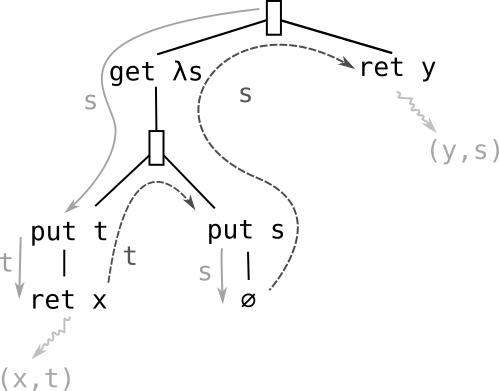
\includegraphics[scale=0.7]{sections/putR}
  \caption{Illustration of state-restoring put}
  \label{fig:putR}
\end{figure}


To help build understanding for \ensuremath{\Varid{put}_{\scaleobj{0.7}{\sf R}}},
Figure~\ref{fig:putR} shows the flow of execution for the expression
\ensuremath{(\Varid{put}_{\scaleobj{0.7}{\sf R}}\;\Varid{t}\mathbin{\hstretch{0.7}{>\!\!>}}\Varid{ret}\;\Varid{x})\mathbin{\talloblong}\Varid{ret}\;\Varid{y}}. Initially, the state is \ensuremath{\Varid{s}}; it gets
modified to \ensuremath{\Varid{t}} at the \ensuremath{\Varid{put}\;\Varid{t}} node after which the value \ensuremath{\Varid{x}} is output
with the working state \ensuremath{\Varid{t}}.
Then, we backtrack (since we're using global-state semantics, the state
modification caused by \ensuremath{\Varid{put}\;\Varid{t}} is not reversed), arriving at \ensuremath{\Varid{put}\;\Varid{s}}, which
resets the state to \ensuremath{\Varid{s}}, immediately fails, and backtracks to the right
branch of the topmost \ensuremath{(\talloblong)}. There the value \ensuremath{\Varid{y}} is output with working
state \ensuremath{\Varid{s}}.

For some further intuition about \ensuremath{\Varid{put}_{\scaleobj{0.7}{\sf R}}}, consider \ensuremath{\Varid{put}_{\scaleobj{0.7}{\sf R}}\;\Varid{s}\mathbin{\hstretch{0.7}{>\!\!>}}\Varid{comp}} where \ensuremath{\Varid{comp}} is some arbitrary computation:
\begin{hscode}\SaveRestoreHook
\column{B}{@{}>{\hspre}l<{\hspost}@{}}%
\column{7}{@{}>{\hspre}l<{\hspost}@{}}%
\column{9}{@{}>{\hspre}l<{\hspost}@{}}%
\column{E}{@{}>{\hspre}l<{\hspost}@{}}%
\>[7]{}\Varid{put}_{\scaleobj{0.7}{\sf R}}\;\Varid{s}\mathbin{\hstretch{0.7}{>\!\!>}}\Varid{comp}{}\<[E]%
\\
\>[B]{}\mathbin{=}{}\<[7]%
\>[7]{}(\Varid{get}\mathrel{\hstretch{0.7}{>\!\!>\!\!=}}\lambda \Varid{s}_{0}\to \Varid{put}\;\Varid{s}\mathbin{\talloblong}\Varid{side}\;(\Varid{put}\;\Varid{s}_{0}))\mathbin{\hstretch{0.7}{>\!\!>}}\Varid{comp}{}\<[E]%
\\
\>[B]{}\mathbin{=}{}\<[9]%
\>[9]{}\mbox{\commentbegin  monad law, left-distributivity \eqref{eq:bind-mplus-dist}  \commentend}{}\<[E]%
\\
\>[B]{}\hsindent{7}{}\<[7]%
\>[7]{}\Varid{get}\mathrel{\hstretch{0.7}{>\!\!>\!\!=}}\lambda \Varid{s}_{0}\to (\Varid{put}\;\Varid{s}\mathbin{\hstretch{0.7}{>\!\!>}}\Varid{comp})\mathbin{\talloblong}(\Varid{side}\;(\Varid{put}\;\Varid{s}_{0})\mathbin{\hstretch{0.7}{>\!\!>}}\Varid{comp}){}\<[E]%
\\
\>[B]{}\mathbin{=}{}\<[9]%
\>[9]{}\mbox{\commentbegin  by \eqref{eq:bind-mzero-zero}, \ensuremath{\emptyset\mathbin{\hstretch{0.7}{>\!\!>}}\Varid{comp}\mathrel{=}\emptyset}  \commentend}{}\<[E]%
\\
\>[B]{}\hsindent{7}{}\<[7]%
\>[7]{}\Varid{get}\mathrel{\hstretch{0.7}{>\!\!>\!\!=}}\lambda \Varid{s}_{0}\to (\Varid{put}\;\Varid{s}\mathbin{\hstretch{0.7}{>\!\!>}}\Varid{comp})\mathbin{\talloblong}\Varid{side}\;(\Varid{put}\;\Varid{s}_{0})~~.{}\<[E]%
\ColumnHook
\end{hscode}\resethooks
Thanks to left-distributivity \eqref{eq:bind-mplus-dist}, \ensuremath{(\mathbin{\hstretch{0.7}{>\!\!>}}\Varid{comp})} is promoted into \ensuremath{(\talloblong)}.
Furthermore, the \ensuremath{(\mathbin{\hstretch{0.7}{>\!\!>}}\Varid{comp})} after \ensuremath{\Varid{side}\;(\Varid{put}\;\Varid{s}_{0})} is discarded by
\eqref{eq:bind-mzero-zero}.
In words, \ensuremath{\Varid{put}_{\scaleobj{0.7}{\sf R}}\;\Varid{s}\mathbin{\hstretch{0.7}{>\!\!>}}\Varid{comp}} saves the current state, computes \ensuremath{\Varid{comp}} using state \ensuremath{\Varid{s}}, and restores the saved state!
The subscript \ensuremath{\Conid{R}} stands for ``restore.''
Note also that \ensuremath{(\Varid{put}_{\scaleobj{0.7}{\sf R}}\;\Varid{s}\mathbin{\hstretch{0.7}{>\!\!>}}\Varid{m}_{1})\mathbin{\hstretch{0.7}{>\!\!>}}\Varid{m}_{2})\mathrel{=}\Varid{put}_{\scaleobj{0.7}{\sf R}}\;\Varid{s}\mathbin{\hstretch{0.7}{>\!\!>}}(\Varid{m}_{1}\mathbin{\hstretch{0.7}{>\!\!>}}\Varid{m}_{2})} --- the state restoration happens in the end.

The behaviour of \ensuremath{\Varid{put}_{\scaleobj{0.7}{\sf R}}}, however, is still rather tricky. It is instructive comparing
\begin{enumerate}[label=(\alph*)]
\item \ensuremath{\Varid{return}\;\Varid{x}},  \label{ex:putR-pitfalls-1}
\item \ensuremath{\Varid{put}\;\Varid{s}\mathbin{\hstretch{0.7}{>\!\!>}}\Varid{return}\;\Varid{x}}, and \label{ex:putR-pitfalls-2}
\item \ensuremath{\Varid{put}_{\scaleobj{0.7}{\sf R}}\;\Varid{s}\mathbin{\hstretch{0.7}{>\!\!>}}\Varid{return}\;\Varid{x}}. \label{ex:putR-pitfalls-3}
\end{enumerate}
When run in initial state \ensuremath{\Varid{s}_{0}}, they all yield \ensuremath{\Varid{x}} as the result.
The final states after running \ref{ex:putR-pitfalls-1}, \ref{ex:putR-pitfalls-2} and \ref{ex:putR-pitfalls-3} are \ensuremath{\Varid{s}_{0}}, \ensuremath{\Varid{s}} and \ensuremath{\Varid{s}_{0}}, respectively.
However, \ref{ex:putR-pitfalls-3} does {\em not} behave identically to \ref{ex:putR-pitfalls-1} in all contexts!
For example, in the context \ensuremath{(\mathbin{\hstretch{0.7}{>\!\!>}}\Varid{get})}, we can tell them apart:
\ensuremath{\Varid{return}\;\Varid{x}\mathbin{\hstretch{0.7}{>\!\!>}}\Varid{get}} returns \ensuremath{\Varid{s}_{0}}, while \ensuremath{\Varid{put}_{\scaleobj{0.7}{\sf R}}\;\Varid{s}\mathbin{\hstretch{0.7}{>\!\!>}}\Varid{return}\;\Varid{x}\mathbin{\hstretch{0.7}{>\!\!>}}\Varid{get}} returns \ensuremath{\Varid{s}}, even though the program yields final state \ensuremath{\Varid{s}_{0}}.

We wish that \ensuremath{\Varid{put}_{\scaleobj{0.7}{\sf R}}}, when run with a global state, satisfies laws \eqref{eq:put-put} through \eqref{eq:mzero-bind-zero} ---
the state laws and the \emph{local} state laws.
If so, one could take a program written for a local state monad, replace all occurrences of \ensuremath{\Varid{put}} by \ensuremath{\Varid{put}_{\scaleobj{0.7}{\sf R}}}, and run the program with a global state.
Unfortunately this is not the case: \ensuremath{\Varid{put}_{\scaleobj{0.7}{\sf R}}} does satisfy \ensuremath{\Varid{put}}-\ensuremath{\Varid{put}}~\eqref{eq:put-put} and \ensuremath{\Varid{put}}-\ensuremath{\Varid{get}}~\eqref{eq:put-get}, but \ensuremath{\Varid{get}}-\ensuremath{\Varid{put}}~\eqref{eq:get-put} fails ---
\ensuremath{\Varid{get}\mathrel{\hstretch{0.7}{>\!\!>\!\!=}}\Varid{put}_{\scaleobj{0.7}{\sf R}}} and \ensuremath{\Varid{return}\;()} can be
told apart by some contexts, for example \ensuremath{(\mathbin{\hstretch{0.7}{>\!\!>}}\Varid{put}\;\Varid{t})}.
To see that, we calculate:
\begin{hscode}\SaveRestoreHook
\column{B}{@{}>{\hspre}c<{\hspost}@{}}%
\column{BE}{@{}l@{}}%
\column{4}{@{}>{\hspre}l<{\hspost}@{}}%
\column{5}{@{}>{\hspre}l<{\hspost}@{}}%
\column{E}{@{}>{\hspre}l<{\hspost}@{}}%
\>[4]{}(\Varid{get}\mathrel{\hstretch{0.7}{>\!\!>\!\!=}}\Varid{put}_{\scaleobj{0.7}{\sf R}})\mathbin{\hstretch{0.7}{>\!\!>}}\Varid{put}\;\Varid{t}{}\<[E]%
\\
\>[B]{}\mathrel{=}{}\<[BE]%
\>[4]{}(\Varid{get}\mathrel{\hstretch{0.7}{>\!\!>\!\!=}}\lambda \Varid{s}\to \Varid{get}\mathrel{\hstretch{0.7}{>\!\!>\!\!=}}\lambda \Varid{s}_{0}\to \Varid{put}\;\Varid{s}\mathbin{\talloblong}\Varid{side}\;(\Varid{put}\;\Varid{s}_{0}))\mathbin{\hstretch{0.7}{>\!\!>}}\Varid{put}\;\Varid{t}{}\<[E]%
\\
\>[B]{}\mathrel{=}{}\<[BE]%
\>[5]{}\mbox{\commentbegin  \ensuremath{\Varid{get}}-\ensuremath{\Varid{get}}  \commentend}{}\<[E]%
\\
\>[B]{}\hsindent{4}{}\<[4]%
\>[4]{}(\Varid{get}\mathrel{\hstretch{0.7}{>\!\!>\!\!=}}\lambda \Varid{s}\to \Varid{put}\;\Varid{s}\mathbin{\talloblong}\Varid{side}\;(\Varid{put}\;\Varid{s}))\mathbin{\hstretch{0.7}{>\!\!>}}\Varid{put}\;\Varid{t}{}\<[E]%
\\
\>[B]{}\mathrel{=}{}\<[BE]%
\>[5]{}\mbox{\commentbegin  monad laws, left-distributivity  \commentend}{}\<[E]%
\\
\>[B]{}\hsindent{4}{}\<[4]%
\>[4]{}\Varid{get}\mathrel{\hstretch{0.7}{>\!\!>\!\!=}}\lambda \Varid{s}\to (\Varid{put}\;\Varid{s}\mathbin{\hstretch{0.7}{>\!\!>}}\Varid{put}\;\Varid{t})\mathbin{\talloblong}\Varid{side}\;(\Varid{put}\;\Varid{s}){}\<[E]%
\\
\>[B]{}\mathrel{=}{}\<[BE]%
\>[5]{}\mbox{\commentbegin  \ensuremath{\Varid{put}}-\ensuremath{\Varid{put}}  \commentend}{}\<[E]%
\\
\>[B]{}\hsindent{4}{}\<[4]%
\>[4]{}\Varid{get}\mathrel{\hstretch{0.7}{>\!\!>\!\!=}}\lambda \Varid{s}\to \Varid{put}\;\Varid{t}\mathbin{\talloblong}\Varid{side}\;(\Varid{put}\;\Varid{s})~~.{}\<[E]%
\ColumnHook
\end{hscode}\resethooks
Meanwhile, \ensuremath{\Varid{return}\;()\mathbin{\hstretch{0.7}{>\!\!>}}\Varid{put}\;\Varid{t}\mathrel{=}\Varid{put}\;\Varid{t}}, which does not behave in the same way as \ensuremath{\Varid{get}\mathrel{\hstretch{0.7}{>\!\!>\!\!=}}\lambda \Varid{s}\to \Varid{put}\;\Varid{t}\mathbin{\talloblong}\Varid{side}\;(\Varid{put}\;\Varid{s})} when $s \neq t$.

In a global-state setting, the left-distributivity law \eqref{eq:bind-mplus-dist} makes it tricky to reason about combinations of \ensuremath{(\talloblong)} and \ensuremath{(\mathrel{\hstretch{0.7}{>\!\!>\!\!=}})} operators.
Suppose we have a program \ensuremath{(\Varid{m}\mathbin{\talloblong}\Varid{n})}, and we construct an extended program by binding a continuation \ensuremath{\Varid{f}} to it such that we get \ensuremath{(\Varid{m}\mathbin{\talloblong}\Varid{n})\mathrel{\hstretch{0.7}{>\!\!>\!\!=}}\Varid{f}} (where \ensuremath{\Varid{f}} might modify the state).
Under global-state semantics, the evaluation of the right branch is influenced by the state modifications performed by evaluating the left branch.
So by \eqref{eq:bind-mplus-dist}, this means that when we get to evaluating the \ensuremath{\Varid{n}} subprogram in the extended program, it will do so with a different initial state (the one obtained after running \ensuremath{\Varid{m}\mathrel{\hstretch{0.7}{>\!\!>\!\!=}}\Varid{f}}) compaired against the initial state in the original program (the one obtained by running \ensuremath{\Varid{m}}).
In other words, placing our program in a different context changed the meaning of one of its subprograms.
So it is difficult to reason about programs compositionally in this setting --- some properties hold only when we take the entire program into consideration.

It turns out that all properties we need do hold, provided that {\em all} occurrences of \ensuremath{\Varid{put}} are replaced by \ensuremath{\Varid{put}_{\scaleobj{0.7}{\sf R}}} --- problematic contexts such as \ensuremath{\Varid{put}\;\Varid{t}} above are thus ruled out.
However, that ``all \ensuremath{\Varid{put}} are replaced by \ensuremath{\Varid{put}_{\scaleobj{0.7}{\sf R}}}'' is a global property, and to properly talk about it we have to formally define contexts, which is what we will do in Section~\ref{sec:ctxt-trans}.

\section{Laws and Translation for Global State Monad}
\label{sec:ctxt-trans}

In this section we give a more formal treatment of non-deterministic global state monad.
We propose laws such a monad should satisfy --- to the best of our knowledge, we are the first to propose these laws.
The laws turn out to be rather intricate.
To make sure that there exists a model, an implementation is proposed in the appendix, and it is verified in Coq that the laws and some additional theorems are satisfied.

The ultimate goal, however, is to show the following property:
given a program written for a local-state monad,
if we replace all occurrences of \ensuremath{\Varid{put}} by \ensuremath{\Varid{put}_{\scaleobj{0.7}{\sf R}}}, the resulting
program yields the same result when run with a global-state monad.
This allows us to painlessly port our previous algorithm to work
with a global state.
To show this we first introduce a syntax for nondeterministic and stateful
monadic programs and contexts.
Then we imbue these programs with global-state semantics.
Finally we define the function that performs the translation just described, and prove that this translation is correct.



\subsection{Programs and Contexts}
\begin{figure}
\begin{mdframed}
\centering
\scriptsize
\subfloat[]{
\begin{minipage}{0.5\textwidth}
\begin{hscode}\SaveRestoreHook
\column{B}{@{}>{\hspre}l<{\hspost}@{}}%
\column{3}{@{}>{\hspre}l<{\hspost}@{}}%
\column{11}{@{}>{\hspre}l<{\hspost}@{}}%
\column{E}{@{}>{\hspre}l<{\hspost}@{}}%
\>[B]{}\mathbf{data}\;\Conid{Prog}\;\Varid{a}\;\mathbf{where}{}\<[E]%
\\
\>[B]{}\hsindent{3}{}\<[3]%
\>[3]{}\Conid{Return}{}\<[11]%
\>[11]{}\mathbin{::}\Varid{a}\to \Conid{Prog}\;\Varid{a}{}\<[E]%
\\
\>[B]{}\hsindent{3}{}\<[3]%
\>[3]{}\emptyset{}\<[11]%
\>[11]{}\mathbin{::}\Conid{Prog}\;\Varid{a}{}\<[E]%
\\
\>[B]{}\hsindent{3}{}\<[3]%
\>[3]{}(\talloblong){}\<[11]%
\>[11]{}\mathbin{::}\Conid{Prog}\;\Varid{a}\to \Conid{Prog}\;\Varid{a}\to \Conid{Prog}\;\Varid{a}{}\<[E]%
\\
\>[B]{}\hsindent{3}{}\<[3]%
\>[3]{}\Conid{Get}{}\<[11]%
\>[11]{}\mathbin{::}(\Conid{S}\to \Conid{Prog}\;\Varid{a})\to \Conid{Prog}\;\Varid{a}{}\<[E]%
\\
\>[B]{}\hsindent{3}{}\<[3]%
\>[3]{}\Conid{Put}{}\<[11]%
\>[11]{}\mathbin{::}\Conid{S}\to \Conid{Prog}\;\Varid{a}\to \Conid{Prog}\;\Varid{a}{}\<[E]%
\ColumnHook
\end{hscode}\resethooks
\end{minipage}
}
\subfloat[]{
  \begin{minipage}{0.5\textwidth}
    \begin{hscode}\SaveRestoreHook
\column{B}{@{}>{\hspre}l<{\hspost}@{}}%
\column{7}{@{}>{\hspre}l<{\hspost}@{}}%
\column{9}{@{}>{\hspre}l<{\hspost}@{}}%
\column{14}{@{}>{\hspre}l<{\hspost}@{}}%
\column{E}{@{}>{\hspre}l<{\hspost}@{}}%
\>[7]{}\mathbf{data}\;\Conid{Env}\;(\Varid{l}\mathbin{::}[\mskip1.5mu \mathbin{*}\mskip1.5mu])\;\mathbf{where}{}\<[E]%
\\
\>[7]{}\hsindent{2}{}\<[9]%
\>[9]{}\Conid{Nil}{}\<[14]%
\>[14]{}\mathbin{::}\Conid{Env}\;`[]{}\<[E]%
\\
\>[7]{}\hsindent{2}{}\<[9]%
\>[9]{}\Conid{Cons}\mathbin{::}\Varid{a}\to \Conid{Env}\;\Varid{l}\to \Conid{Env}\;(\Varid{a}\mathbin{:}\Varid{l}){}\<[E]%
\\[\blanklineskip]%
\>[7]{}\mathbf{type}\;\Conid{OProg}\;\Varid{e}\;\Varid{a}\mathrel{=}\Conid{Env}\;\Varid{e}\to \Conid{Prog}\;\Varid{a}{}\<[E]%
\ColumnHook
\end{hscode}\resethooks
  \end{minipage}
}
\quad
\subfloat[]{
  \begin{minipage}{0.5\textwidth}
    \begin{hscode}\SaveRestoreHook
\column{B}{@{}>{\hspre}l<{\hspost}@{}}%
\column{5}{@{}>{\hspre}l<{\hspost}@{}}%
\column{7}{@{}>{\hspre}l<{\hspost}@{}}%
\column{15}{@{}>{\hspre}l<{\hspost}@{}}%
\column{E}{@{}>{\hspre}l<{\hspost}@{}}%
\>[5]{}\mathbf{data}\;\Conid{Ctx}\;\Varid{e}_{1}\;\Varid{a}\;\Varid{e}_{2}\;\Varid{b}\;\mathbf{where}{}\<[E]%
\\
\>[5]{}\hsindent{2}{}\<[7]%
\>[7]{}\square{}\<[15]%
\>[15]{}\mathbin{::}\Conid{Ctx}\;\Varid{e}\;\Varid{a}\;\Varid{e}\;\Varid{a}{}\<[E]%
\\
\>[5]{}\hsindent{2}{}\<[7]%
\>[7]{}\Conid{COr1}{}\<[15]%
\>[15]{}\mathbin{::}\Conid{Ctx}\;\Varid{e}_{1}\;\Varid{a}\;\Varid{e}_{2}\;\Varid{b}\to \Conid{OProg}\;\Varid{e}_{2}\;\Varid{b}{}\<[E]%
\\
\>[15]{}\to \Conid{Ctx}\;\Varid{e}_{1}\;\Varid{a}\;\Varid{e}_{2}\;\Varid{b}{}\<[E]%
\\
\>[5]{}\hsindent{2}{}\<[7]%
\>[7]{}\Conid{COr2}{}\<[15]%
\>[15]{}\mathbin{::}\Conid{OProg}\;\Varid{e}_{2}\;\Varid{b}\to \Conid{Ctx}\;\Varid{e}_{1}\;\Varid{a}\;\Varid{e}_{2}\;\Varid{b}{}\<[E]%
\\
\>[15]{}\to \Conid{Ctx}\;\Varid{e}_{1}\;\Varid{a}\;\Varid{e}_{2}\;\Varid{b}{}\<[E]%
\\
\>[5]{}\hsindent{2}{}\<[7]%
\>[7]{}\Conid{CPut}{}\<[15]%
\>[15]{}\mathbin{::}(\Conid{Env}\;\Varid{e}_{2}\to \Conid{S})\to \Conid{Ctx}\;\Varid{e}_{1}\;\Varid{a}\;\Varid{e}_{2}\;\Varid{b}{}\<[E]%
\\
\>[15]{}\to \Conid{Ctx}\;\Varid{e}_{1}\;\Varid{a}\;\Varid{e}_{2}\;\Varid{b}{}\<[E]%
\\
\>[5]{}\hsindent{2}{}\<[7]%
\>[7]{}\Conid{CGet}{}\<[15]%
\>[15]{}\mathbin{::}(\Conid{S}\to \Conid{Bool})\to \Conid{Ctx}\;\Varid{e}_{1}\;\Varid{a}\;(\Conid{S}\mathbin{:}\Varid{e}_{2})\;\Varid{b}{}\<[E]%
\\
\>[15]{}\to (\Conid{S}\to \Conid{OProg}\;\Varid{e}_{2}\;\Varid{b})\to \Conid{Ctx}\;\Varid{e}_{1}\;\Varid{a}\;\Varid{e}_{2}\;\Varid{b}{}\<[E]%
\\
\>[5]{}\hsindent{2}{}\<[7]%
\>[7]{}\Conid{CBind1}{}\<[15]%
\>[15]{}\mathbin{::}\Conid{Ctx}\;\Varid{e}_{1}\;\Varid{a}\;\Varid{e}_{2}\;\Varid{b}\to (\Varid{b}\to \Conid{OProg}\;\Varid{e}_{2}\;\Varid{c}){}\<[E]%
\\
\>[15]{}\to \Conid{Ctx}\;\Varid{e}_{1}\;\Varid{a}\;\Varid{e}_{2}\;\Varid{c}{}\<[E]%
\\
\>[5]{}\hsindent{2}{}\<[7]%
\>[7]{}\Conid{CBind2}{}\<[15]%
\>[15]{}\mathbin{::}\Conid{OProg}\;\Varid{e}_{2}\;\Varid{a}\to \Conid{Ctx}\;\Varid{e}_{1}\;\Varid{b}\;(\Varid{a}\mathbin{:}\Varid{e}_{2})\;\Varid{c}{}\<[E]%
\\
\>[15]{}\to \Conid{Ctx}\;\Varid{e}_{1}\;\Varid{b}\;\Varid{e}_{2}\;\Varid{c}{}\<[E]%
\ColumnHook
\end{hscode}\resethooks
  \end{minipage}
}
\subfloat[]{
  \begin{minipage}{0.5\textwidth}
    \begin{hscode}\SaveRestoreHook
\column{B}{@{}>{\hspre}l<{\hspost}@{}}%
\column{7}{@{}>{\hspre}c<{\hspost}@{}}%
\column{7E}{@{}l@{}}%
\column{14}{@{}>{\hspre}l<{\hspost}@{}}%
\column{E}{@{}>{\hspre}l<{\hspost}@{}}%
\>[7]{}\Varid{run}{}\<[7E]%
\>[14]{}\mathbin{::}\Conid{Prog}\;\Varid{a}\to \Conid{Dom}\;\Varid{a}{}\<[E]%
\\
\>[7]{}\scaleobj{0.8}{\langle}\Varid{ret}\scaleobj{0.8}{\rangle}{}\<[7E]%
\>[14]{}\mathbin{::}\Varid{a}\to \Conid{Dom}\;\Varid{a}{}\<[E]%
\\
\>[7]{}\scaleobj{0.8}{\langle}\varnothing\scaleobj{0.8}{\rangle}{}\<[7E]%
\>[14]{}\mathbin{::}\Conid{Dom}\;\Varid{a}{}\<[E]%
\\
\>[7]{}\mathbin{\scaleobj{0.8}{\langle[\!]\rangle}}{}\<[7E]%
\>[14]{}\mathbin{::}\Conid{Dom}\;\Varid{a}\to \Conid{Dom}\;\Varid{a}\to \Conid{Dom}\;\Varid{a}{}\<[E]%
\\
\>[7]{}\scaleobj{0.8}{\langle}\Varid{get}\scaleobj{0.8}{\rangle}{}\<[7E]%
\>[14]{}\mathbin{::}(\Conid{S}\to \Conid{Dom}\;\Varid{a})\to \Conid{Dom}\;\Varid{a}{}\<[E]%
\\
\>[7]{}\scaleobj{0.8}{\langle}\Varid{put}\scaleobj{0.8}{\rangle}{}\<[7E]%
\>[14]{}\mathbin{::}\Conid{S}\to \Conid{Dom}\;\Varid{a}\to \Conid{Dom}\;\Varid{a}{}\<[E]%
\ColumnHook
\end{hscode}\resethooks
  \end{minipage}
}
\quad
\end{mdframed}
\caption{(a) Syntax for programs. (b) Environments and open programs. (c) Syntax
  for contexts. (d) Semantic domain.}
\label{fig:context-semantics}
\end{figure}
In the previous sections we have been mixing syntax and semantics,
which we avoid in this section by defining the program syntax as a free monad.
This way we avoid the need for a type-level distinction between programs
with local-state semantics and programs with global-state semantics.
Figure~\ref{fig:context-semantics}(a) defines a syntax for
nondeterministic, stateful, closed programs \ensuremath{\Conid{Prog}}, where
the \ensuremath{\Conid{Get}} and \ensuremath{\Conid{Put}} constructors take continuations as arguments, and
the \ensuremath{(\mathrel{\hstretch{0.7}{>\!\!>\!\!=}})} operator is defined as follows:
\begin{samepage}
\begin{hscode}\SaveRestoreHook
\column{B}{@{}>{\hspre}l<{\hspost}@{}}%
\column{3}{@{}>{\hspre}l<{\hspost}@{}}%
\column{18}{@{}>{\hspre}l<{\hspost}@{}}%
\column{E}{@{}>{\hspre}l<{\hspost}@{}}%
\>[3]{}(\mathrel{\hstretch{0.7}{>\!\!>\!\!=}})\mathbin{::}\Conid{Prog}\;\Varid{a}\to (\Varid{a}\to \Conid{Prog}\;\Varid{b})\to \Conid{Prog}\;\Varid{b}{}\<[E]%
\\
\>[3]{}\Conid{Return}\;\Varid{x}{}\<[18]%
\>[18]{}\mathrel{\hstretch{0.7}{>\!\!>\!\!=}}\Varid{f}\mathrel{=}\Varid{f}\;\Varid{x}{}\<[E]%
\\
\>[3]{}\emptyset{}\<[18]%
\>[18]{}\mathrel{\hstretch{0.7}{>\!\!>\!\!=}}\Varid{f}\mathrel{=}\emptyset{}\<[E]%
\\
\>[3]{}(\Varid{m}\mathbin{\talloblong}\Varid{n}){}\<[18]%
\>[18]{}\mathrel{\hstretch{0.7}{>\!\!>\!\!=}}\Varid{f}\mathrel{=}(\Varid{m}\mathrel{\hstretch{0.7}{>\!\!>\!\!=}}\Varid{f})\mathbin{\talloblong}(\Varid{n}\mathrel{\hstretch{0.7}{>\!\!>\!\!=}}\Varid{f}){}\<[E]%
\\
\>[3]{}\Conid{Get}\;\Varid{k}{}\<[18]%
\>[18]{}\mathrel{\hstretch{0.7}{>\!\!>\!\!=}}\Varid{f}\mathrel{=}\Conid{Get}\;(\lambda \Varid{s}\to \Varid{k}\;\Varid{s}\mathrel{\hstretch{0.7}{>\!\!>\!\!=}}\Varid{f}){}\<[E]%
\\
\>[3]{}\Conid{Put}\;\Varid{s}\;\Varid{m}{}\<[18]%
\>[18]{}\mathrel{\hstretch{0.7}{>\!\!>\!\!=}}\Varid{f}\mathrel{=}\Conid{Put}\;\Varid{s}\;(\Varid{m}\mathrel{\hstretch{0.7}{>\!\!>\!\!=}}\Varid{k})~~.{}\<[E]%
\ColumnHook
\end{hscode}\resethooks
\end{samepage}%
One can see that \ensuremath{(\mathrel{\hstretch{0.7}{>\!\!>\!\!=}})} is defined as a purely syntactical manipulation, and
its definition has laws \eqref{eq:bind-mplus-dist} and
\eqref{eq:bind-mzero-zero} built-in.

The meaning of such a monadic program is determined by a semantic domain of our
choosing, which we denote with \ensuremath{\Conid{Dom}}, and its corresponding
domain operators \ensuremath{\scaleobj{0.8}{\langle}\Varid{ret}\scaleobj{0.8}{\rangle}}, \ensuremath{\scaleobj{0.8}{\langle}\varnothing\scaleobj{0.8}{\rangle}}, \ensuremath{\scaleobj{0.8}{\langle}\Varid{get}\scaleobj{0.8}{\rangle}}, \ensuremath{\scaleobj{0.8}{\langle}\Varid{put}\scaleobj{0.8}{\rangle}} and \ensuremath{(\mathbin{\scaleobj{0.8}{\langle[\!]\rangle}})}
(see figure~\ref{fig:context-semantics}(d)).
The \ensuremath{\Varid{run}\mathbin{::}\Conid{Prog}\;\Varid{a}\to \Conid{Dom}\;\Varid{a}} function ``runs'' a program \ensuremath{\Conid{Prog}\;\Varid{a}} into a value
in the semantic domain \ensuremath{\Conid{Dom}\;\Varid{a}}:
\begin{samepage}
\begin{hscode}\SaveRestoreHook
\column{B}{@{}>{\hspre}l<{\hspost}@{}}%
\column{22}{@{}>{\hspre}l<{\hspost}@{}}%
\column{E}{@{}>{\hspre}l<{\hspost}@{}}%
\>[B]{}\Varid{run}\;(\Conid{Return}\;\Varid{x}){}\<[22]%
\>[22]{}\mathrel{=}\scaleobj{0.8}{\langle}\Varid{ret}\scaleobj{0.8}{\rangle}\;\Varid{x}{}\<[E]%
\\
\>[B]{}\Varid{run}\;\emptyset{}\<[22]%
\>[22]{}\mathrel{=}\scaleobj{0.8}{\langle}\varnothing\scaleobj{0.8}{\rangle}{}\<[E]%
\\
\>[B]{}\Varid{run}\;(\Varid{m}_{1}\mathbin{\talloblong}\Varid{m}_{2}){}\<[22]%
\>[22]{}\mathrel{=}\Varid{run}\;\Varid{m}_{1}\mathbin{\scaleobj{0.8}{\langle[\!]\rangle}}\Varid{run}\;\Varid{m}_{2}{}\<[E]%
\\
\>[B]{}\Varid{run}\;(\Conid{Get}\;\Varid{k}){}\<[22]%
\>[22]{}\mathrel{=}\scaleobj{0.8}{\langle}\Varid{get}\scaleobj{0.8}{\rangle}\;(\lambda \Varid{s}\to \Varid{run}\;(\Varid{k}\;\Varid{s})){}\<[E]%
\\
\>[B]{}\Varid{run}\;(\Conid{Put}\;\Varid{s}\;\Varid{m}){}\<[22]%
\>[22]{}\mathrel{=}\scaleobj{0.8}{\langle}\Varid{put}\scaleobj{0.8}{\rangle}\;\Varid{s}\;(\Varid{run}\;\Varid{m})~~.{}\<[E]%
\ColumnHook
\end{hscode}\resethooks
\end{samepage}%
Note that no \ensuremath{\mathbin{\scaleobj{0.8}{\langle\hstretch{0.7}{>\!\!>\!\!=}\rangle}}} operator is required to define \ensuremath{\Varid{run}};
in other words, \ensuremath{\Conid{Dom}} need not be a monad.
In fact, as we will see later, we will choose our implementation in such a way
that there does not exist a bind operator for \ensuremath{\Varid{run}}.

\subsection{Modeling Global State Semantics}
\label{sec:model-global-state-sem}
We impose the laws upon \ensuremath{\Conid{Dom}} and the domain operators to ensure the semantics of a
non-backtracking (global-state),
nondeterministic, stateful computation for our programs.
Naturally, we need laws analogous to the state laws and nondeterminism laws to
hold for our semantic domain.
As it is not required that a bind operator
(\ensuremath{(\mathrel{\hstretch{0.7}{>\!\!>\!\!=}})\mathbin{::}\Conid{Dom}\;\Varid{a}\to (\Varid{a}\to \Conid{Dom}\;\Varid{b})\to \Conid{Dom}\;\Varid{b}}) can be defined for the semantic
domain (and we will later argue that it \emph{cannot} be defined for the domain,
given the laws we impose on it), the state laws
(\eqref{eq:put-put} through \eqref{eq:get-get})
must be reformulated to fit the continuation-passing style of the semantic domain
operators.
\begin{align}
  \ensuremath{\scaleobj{0.8}{\langle}\Varid{put}\scaleobj{0.8}{\rangle}\;\Varid{s}\;(\scaleobj{0.8}{\langle}\Varid{put}\scaleobj{0.8}{\rangle}\;\Varid{t}\;\Varid{p})} &= \ensuremath{\scaleobj{0.8}{\langle}\Varid{put}\scaleobj{0.8}{\rangle}\;\Varid{t}\;\Varid{p}} \mbox{~~,} \label{eq:put-put-g-d} \\
  \ensuremath{\scaleobj{0.8}{\langle}\Varid{put}\scaleobj{0.8}{\rangle}\;\Varid{s}\;(\scaleobj{0.8}{\langle}\Varid{get}\scaleobj{0.8}{\rangle}\;\Varid{k})} &= \ensuremath{\scaleobj{0.8}{\langle}\Varid{put}\scaleobj{0.8}{\rangle}\;\Varid{s}\;(\Varid{k}\;\Varid{s})} \mbox{~~,} \label{eq:put-get-g-d} \\
  \ensuremath{\scaleobj{0.8}{\langle}\Varid{get}\scaleobj{0.8}{\rangle}\;(\lambda \Varid{s}\to \scaleobj{0.8}{\langle}\Varid{put}\scaleobj{0.8}{\rangle}\;\Varid{s}\;\Varid{m})} &= \ensuremath{\Varid{m}} \mbox{~~,} \label{eq:get-put-g-d} \\
  \ensuremath{\scaleobj{0.8}{\langle}\Varid{get}\scaleobj{0.8}{\rangle}\;(\lambda \Varid{s}\to \scaleobj{0.8}{\langle}\Varid{get}\scaleobj{0.8}{\rangle}\;(\lambda \Varid{t}\to \Varid{k}\;\Varid{s}\;\Varid{t}))} &= \ensuremath{\scaleobj{0.8}{\langle}\Varid{get}\scaleobj{0.8}{\rangle}\;(\lambda \Varid{s}\to \Varid{k}\;\Varid{s}\;\Varid{s})} \mbox{~~.} \label{eq:get-get-g-d}
\end{align}
As for the nondeterminism laws
(\eqref{eq:mplus-assoc}, \eqref{eq:mzero-mplus}, \eqref{eq:bind-mplus-dist},
\eqref{eq:bind-mzero-zero}),
we can simply omit the ones that mention at the semantic level \ensuremath{(\mathrel{\hstretch{0.7}{>\!\!>\!\!=}})}
as these are proven at the syntactic level: their proof follows immediately
from \ensuremath{\Conid{Prog}}'s definition of \ensuremath{(\mathrel{\hstretch{0.7}{>\!\!>\!\!=}})}.
\begin{align}
  &\ensuremath{(\Varid{m}\mathbin{\scaleobj{0.8}{\langle[\!]\rangle}}\Varid{n})\mathbin{\scaleobj{0.8}{\langle[\!]\rangle}}\Varid{p}} = \ensuremath{\Varid{m}\mathbin{\scaleobj{0.8}{\langle[\!]\rangle}}(\Varid{n}\mathbin{\scaleobj{0.8}{\langle[\!]\rangle}}\Varid{p})} \mbox{~~,} \\
  &\ensuremath{\scaleobj{0.8}{\langle}\varnothing\scaleobj{0.8}{\rangle}\mathbin{\scaleobj{0.8}{\langle[\!]\rangle}}\Varid{m}} = \ensuremath{\Varid{m}\mathbin{\scaleobj{0.8}{\langle[\!]\rangle}}\scaleobj{0.8}{\langle}\varnothing\scaleobj{0.8}{\rangle}} = \ensuremath{\Varid{m}} \mbox{~~.}
\end{align}

We also reformulate the global-state law~\eqref{eq:put-or}:
\begin{align}
\ensuremath{\scaleobj{0.8}{\langle}\Varid{put}\scaleobj{0.8}{\rangle}\;\Varid{s}\;\Varid{p}\mathbin{\scaleobj{0.8}{\langle[\!]\rangle}}\Varid{q}}        &= \ensuremath{\scaleobj{0.8}{\langle}\Varid{put}\scaleobj{0.8}{\rangle}\;\Varid{s}\;(\Varid{p}\mathbin{\scaleobj{0.8}{\langle[\!]\rangle}}\Varid{q})} \mbox{~~.}\label{eq:put-or-g-d}
\end{align}
%In Section~\ref{sec:laws-global-state} we also mentioned that a law should exist
%which mandates a limited form of right-distribitivity which only holds on a
%global level.
%The continuation-passing style of our semantic domain operators allows us to
%express a weaker version of this global property (which suffices for our goals)
%as follows:
It turns out that, apart from the {\bf put-or} law,
our proofs require certain additional properties regarding commutativity and
distributivity which we introduce here:
\begin{align}
\begin{split}
\ensuremath{\scaleobj{0.8}{\langle}\Varid{get}\scaleobj{0.8}{\rangle}\;(\lambda \Varid{s}\to \scaleobj{0.8}{\langle}\Varid{put}\scaleobj{0.8}{\rangle}\;(\Varid{t}\;\Varid{s})\;\Varid{p}\mathbin{\scaleobj{0.8}{\langle[\!]\rangle}}\scaleobj{0.8}{\langle}\Varid{put}\scaleobj{0.8}{\rangle}\;(\Varid{u}\;\Varid{s})\;\Varid{q}\mathbin{\scaleobj{0.8}{\langle[\!]\rangle}}\scaleobj{0.8}{\langle}\Varid{put}\scaleobj{0.8}{\rangle}\;\Varid{s}\;\scaleobj{0.8}{\langle}\varnothing\scaleobj{0.8}{\rangle})} = \\
~~~~~~\ensuremath{\scaleobj{0.8}{\langle}\Varid{get}\scaleobj{0.8}{\rangle}\;(\lambda \Varid{s}\to \scaleobj{0.8}{\langle}\Varid{put}\scaleobj{0.8}{\rangle}\;(\Varid{u}\;\Varid{s})\;\Varid{q}\mathbin{\scaleobj{0.8}{\langle[\!]\rangle}}\scaleobj{0.8}{\langle}\Varid{put}\scaleobj{0.8}{\rangle}\;(\Varid{t}\;\Varid{s})\;\Varid{p}\mathbin{\scaleobj{0.8}{\langle[\!]\rangle}}\scaleobj{0.8}{\langle}\Varid{put}\scaleobj{0.8}{\rangle}\;\Varid{s}\;\scaleobj{0.8}{\langle}\varnothing\scaleobj{0.8}{\rangle})} \mbox {~~,}
\end{split} \label{eq:put-or-comm-g-d} \\
& \ensuremath{\scaleobj{0.8}{\langle}\Varid{put}\scaleobj{0.8}{\rangle}\;\Varid{s}\;(\scaleobj{0.8}{\langle}\Varid{ret}\scaleobj{0.8}{\rangle}\;\Varid{x}\mathbin{\scaleobj{0.8}{\langle[\!]\rangle}}\Varid{p})} = \ensuremath{\scaleobj{0.8}{\langle}\Varid{put}\scaleobj{0.8}{\rangle}\;\Varid{s}\;(\scaleobj{0.8}{\langle}\Varid{ret}\scaleobj{0.8}{\rangle}\;\Varid{x})\mathbin{\scaleobj{0.8}{\langle[\!]\rangle}}\scaleobj{0.8}{\langle}\Varid{put}\scaleobj{0.8}{\rangle}\;\Varid{s}\;\Varid{p}} \mbox{~~.}\label{eq:put-ret-or-g-d}
\end{align}
These laws are not considered general ``global state'' laws, because it is
possible to define reasonable implementations of global state semantics that
violate these laws, and because they are not exclusive to global state
semantics.

The \ensuremath{\mathbin{\scaleobj{0.8}{\langle[\!]\rangle}}} operator is not, in general, commutative in a global state setting.
However, we will require that the order in which results are computed does not
matter.
Furthermore we require that the implementation is agnostic with repect to the
order of \ensuremath{\scaleobj{0.8}{\langle}\Varid{put}\scaleobj{0.8}{\rangle}} operations as long as the exact same results are computed with
the exact same state at the time of their computation.
These properties are enforced by law~\eqref{eq:put-or-comm-g-d}.
Implementations that present the results as an ordered list violate this law,
as are implementations that record the order of proper state changes.

In global-state semantics, \ensuremath{\scaleobj{0.8}{\langle}\Varid{put}\scaleobj{0.8}{\rangle}} operations cannot, in general,
distribute over \ensuremath{\mathbin{\scaleobj{0.8}{\langle[\!]\rangle}}}.
However, an implementation may permit distributivity if certain conditions are
met.
Law~\eqref{eq:put-ret-or-g-d} states that a \ensuremath{\scaleobj{0.8}{\langle}\Varid{put}\scaleobj{0.8}{\rangle}} operation distributes over a
nondeterministic choice if the left branch of that choice simply returns a
value.
An example of an implementation that violates this law would be one that
applies a given function \ensuremath{\Varid{f}\mathbin{::}\Varid{s}\to \Varid{s}} to the state after each return.
Such an implementation would conform to an alternative law
\ensuremath{\scaleobj{0.8}{\langle}\Varid{put}\scaleobj{0.8}{\rangle}\;\Varid{x}\;(\scaleobj{0.8}{\langle}\Varid{ret}\scaleobj{0.8}{\rangle}\;\Varid{w}\mathbin{\scaleobj{0.8}{\langle[\!]\rangle}}\Varid{q})\mathrel{=}\scaleobj{0.8}{\langle}\Varid{put}\scaleobj{0.8}{\rangle}\;\Varid{x}\;(\scaleobj{0.8}{\langle}\Varid{ret}\scaleobj{0.8}{\rangle}\;\Varid{w})\mathbin{\scaleobj{0.8}{\langle[\!]\rangle}}\scaleobj{0.8}{\langle}\Varid{put}\scaleobj{0.8}{\rangle}\;(\Varid{f}\;\Varid{x})\;\Varid{q}}.
Law~\eqref{eq:put-ret-or-g-d} only holds if the implementation of \ensuremath{\Conid{Dom}} does not
permit the definition
of a bind operator \ensuremath{(\mathbin{\scaleobj{0.8}{\langle\hstretch{0.7}{>\!\!>\!\!=}\rangle}})\mathbin{::}\Conid{Dom}\;\Varid{a}\to (\Varid{a}\to \Conid{Dom}\;\Varid{b})\to \Conid{Dom}\;\Varid{b}}.
Consider for instance the following program:
\begin{hscode}\SaveRestoreHook
\column{B}{@{}>{\hspre}l<{\hspost}@{}}%
\column{3}{@{}>{\hspre}l<{\hspost}@{}}%
\column{E}{@{}>{\hspre}l<{\hspost}@{}}%
\>[3]{}\scaleobj{0.8}{\langle}\Varid{put}\scaleobj{0.8}{\rangle}\;\Varid{x}\;(\scaleobj{0.8}{\langle}\Varid{ret}\scaleobj{0.8}{\rangle}\;\Varid{w}\mathbin{\scaleobj{0.8}{\langle[\!]\rangle}}\scaleobj{0.8}{\langle}\Varid{get}\scaleobj{0.8}{\rangle}\;\scaleobj{0.8}{\langle}\Varid{ret}\scaleobj{0.8}{\rangle})\mathbin{\scaleobj{0.8}{\langle\hstretch{0.7}{>\!\!>\!\!=}\rangle}}\lambda \Varid{z}\to \scaleobj{0.8}{\langle}\Varid{put}\scaleobj{0.8}{\rangle}\;\Varid{y}\;(\scaleobj{0.8}{\langle}\Varid{ret}\scaleobj{0.8}{\rangle}\;\Varid{z})~~.{}\<[E]%
\ColumnHook
\end{hscode}\resethooks
If \eqref{eq:put-ret-or-g-d} holds, this program should be equal to
\begin{hscode}\SaveRestoreHook
\column{B}{@{}>{\hspre}l<{\hspost}@{}}%
\column{3}{@{}>{\hspre}l<{\hspost}@{}}%
\column{E}{@{}>{\hspre}l<{\hspost}@{}}%
\>[3]{}(\scaleobj{0.8}{\langle}\Varid{put}\scaleobj{0.8}{\rangle}\;\Varid{x}\;(\scaleobj{0.8}{\langle}\Varid{ret}\scaleobj{0.8}{\rangle}\;\Varid{w})\mathbin{\scaleobj{0.8}{\langle[\!]\rangle}}\scaleobj{0.8}{\langle}\Varid{put}\scaleobj{0.8}{\rangle}\;\Varid{x}\;(\scaleobj{0.8}{\langle}\Varid{get}\scaleobj{0.8}{\rangle}\;\scaleobj{0.8}{\langle}\Varid{ret}\scaleobj{0.8}{\rangle}))\mathbin{\scaleobj{0.8}{\langle\hstretch{0.7}{>\!\!>\!\!=}\rangle}}\lambda \Varid{z}\to \scaleobj{0.8}{\langle}\Varid{put}\scaleobj{0.8}{\rangle}\;\Varid{y}\;(\scaleobj{0.8}{\langle}\Varid{ret}\scaleobj{0.8}{\rangle}\;\Varid{z})~~.{}\<[E]%
\ColumnHook
\end{hscode}\resethooks
However, Figure~\ref{fig:put-ret-or-vs-bind} proves that the first program can
be reduced to \ensuremath{\scaleobj{0.8}{\langle}\Varid{put}\scaleobj{0.8}{\rangle}\;\Varid{y}\;(\scaleobj{0.8}{\langle}\Varid{ret}\scaleobj{0.8}{\rangle}\;\Varid{w}\mathbin{\scaleobj{0.8}{\langle[\!]\rangle}}\scaleobj{0.8}{\langle}\Varid{ret}\scaleobj{0.8}{\rangle}\;\Varid{y})},
whereas the second program is equal to
\ensuremath{\scaleobj{0.8}{\langle}\Varid{put}\scaleobj{0.8}{\rangle}\;\Varid{y}\;(\scaleobj{0.8}{\langle}\Varid{ret}\scaleobj{0.8}{\rangle}\;\Varid{w}\mathbin{\scaleobj{0.8}{\langle[\!]\rangle}}\scaleobj{0.8}{\langle}\Varid{ret}\scaleobj{0.8}{\rangle}\;\Varid{x})},
which clearly does not always have the same result.
\begin{figure}
  \centering
  \tiny
  \subfloat[]{
  \begin{minipage}{0.5\textwidth}
    \begin{hscode}\SaveRestoreHook
\column{B}{@{}>{\hspre}l<{\hspost}@{}}%
\column{7}{@{}>{\hspre}l<{\hspost}@{}}%
\column{29}{@{}>{\hspre}l<{\hspost}@{}}%
\column{E}{@{}>{\hspre}l<{\hspost}@{}}%
\>[7]{}\scaleobj{0.8}{\langle}\Varid{put}\scaleobj{0.8}{\rangle}\;\Varid{x}\;(\scaleobj{0.8}{\langle}\Varid{ret}\scaleobj{0.8}{\rangle}\;\Varid{w}\mathbin{\scaleobj{0.8}{\langle[\!]\rangle}}\scaleobj{0.8}{\langle}\Varid{get}\scaleobj{0.8}{\rangle}\;\scaleobj{0.8}{\langle}\Varid{ret}\scaleobj{0.8}{\rangle})\mathbin{\scaleobj{0.8}{\langle\hstretch{0.7}{>\!\!>\!\!=}\rangle}}\lambda \Varid{z}\to \scaleobj{0.8}{\langle}\Varid{put}\scaleobj{0.8}{\rangle}\;\Varid{y}\;(\scaleobj{0.8}{\langle}\Varid{ret}\scaleobj{0.8}{\rangle}\;\Varid{z}){}\<[E]%
\\
\>[7]{}\mathbin{=}\mbox{\commentbegin  definition of \ensuremath{(\mathbin{\scaleobj{0.8}{\langle\hstretch{0.7}{>\!\!>\!\!=}\rangle}})}  \commentend}{}\<[E]%
\\
\>[7]{}\scaleobj{0.8}{\langle}\Varid{put}\scaleobj{0.8}{\rangle}\;\Varid{x}\;(\scaleobj{0.8}{\langle}\Varid{put}\scaleobj{0.8}{\rangle}\;\Varid{y}\;(\scaleobj{0.8}{\langle}\Varid{ret}\scaleobj{0.8}{\rangle}\;\Varid{w})\mathbin{\scaleobj{0.8}{\langle[\!]\rangle}}\scaleobj{0.8}{\langle}\Varid{get}\scaleobj{0.8}{\rangle}\;(\lambda \Varid{s}\to \scaleobj{0.8}{\langle}\Varid{put}\scaleobj{0.8}{\rangle}\;\Varid{y}\;(\scaleobj{0.8}{\langle}\Varid{ret}\scaleobj{0.8}{\rangle}\;\Varid{s}))){}\<[E]%
\\
\>[7]{}\mathbin{=}\mbox{\commentbegin  by \eqref{eq:put-or-g-d} and \eqref{eq:put-put-g-d}  \commentend}{}\<[E]%
\\
\>[7]{}\scaleobj{0.8}{\langle}\Varid{put}\scaleobj{0.8}{\rangle}\;\Varid{y}\;(\scaleobj{0.8}{\langle}\Varid{ret}\scaleobj{0.8}{\rangle}\;\Varid{w}\mathbin{\scaleobj{0.8}{\langle[\!]\rangle}}\scaleobj{0.8}{\langle}\Varid{get}\scaleobj{0.8}{\rangle}\;(\lambda \Varid{s}\to \scaleobj{0.8}{\langle}\Varid{put}\scaleobj{0.8}{\rangle}\;\Varid{y}\;(\scaleobj{0.8}{\langle}\Varid{ret}\scaleobj{0.8}{\rangle}\;\Varid{s}))){}\<[E]%
\\
\>[7]{}\mathbin{=}\mbox{\commentbegin  by \eqref{eq:put-ret-or-g-d}  \commentend}{}\<[E]%
\\
\>[7]{}\scaleobj{0.8}{\langle}\Varid{put}\scaleobj{0.8}{\rangle}\;\Varid{y}\;(\scaleobj{0.8}{\langle}\Varid{ret}\scaleobj{0.8}{\rangle}\;\Varid{w})\mathbin{\scaleobj{0.8}{\langle[\!]\rangle}}{}\<[29]%
\>[29]{}\scaleobj{0.8}{\langle}\Varid{put}\scaleobj{0.8}{\rangle}\;\Varid{y}\;(\scaleobj{0.8}{\langle}\Varid{get}\scaleobj{0.8}{\rangle}\;(\lambda \Varid{s}\to \scaleobj{0.8}{\langle}\Varid{put}\scaleobj{0.8}{\rangle}\;\Varid{y}\;(\scaleobj{0.8}{\langle}\Varid{ret}\scaleobj{0.8}{\rangle}\;\Varid{s}))){}\<[E]%
\\
\>[7]{}\mathbin{=}\mbox{\commentbegin  by \eqref{eq:put-get-g-d} and \eqref{eq:put-put-g-d}  \commentend}{}\<[E]%
\\
\>[7]{}\scaleobj{0.8}{\langle}\Varid{put}\scaleobj{0.8}{\rangle}\;\Varid{y}\;(\scaleobj{0.8}{\langle}\Varid{ret}\scaleobj{0.8}{\rangle}\;\Varid{w})\mathbin{\scaleobj{0.8}{\langle[\!]\rangle}}\scaleobj{0.8}{\langle}\Varid{put}\scaleobj{0.8}{\rangle}\;\Varid{y}\;(\scaleobj{0.8}{\langle}\Varid{ret}\scaleobj{0.8}{\rangle}\;\Varid{y}){}\<[E]%
\\
\>[7]{}\mathbin{=}\mbox{\commentbegin  by \eqref{eq:put-ret-or-g-d}  \commentend}{}\<[E]%
\\
\>[7]{}\scaleobj{0.8}{\langle}\Varid{put}\scaleobj{0.8}{\rangle}\;\Varid{y}\;(\scaleobj{0.8}{\langle}\Varid{ret}\scaleobj{0.8}{\rangle}\;\Varid{w}\mathbin{\scaleobj{0.8}{\langle[\!]\rangle}}\scaleobj{0.8}{\langle}\Varid{ret}\scaleobj{0.8}{\rangle}\;\Varid{y}){}\<[E]%
\ColumnHook
\end{hscode}\resethooks
  \end{minipage}
  }
  \subfloat[]{
  \begin{minipage}{0.5\textwidth}
    \begin{hscode}\SaveRestoreHook
\column{B}{@{}>{\hspre}l<{\hspost}@{}}%
\column{7}{@{}>{\hspre}l<{\hspost}@{}}%
\column{9}{@{}>{\hspre}l<{\hspost}@{}}%
\column{E}{@{}>{\hspre}l<{\hspost}@{}}%
\>[7]{}(\scaleobj{0.8}{\langle}\Varid{put}\scaleobj{0.8}{\rangle}\;\Varid{x}\;(\scaleobj{0.8}{\langle}\Varid{ret}\scaleobj{0.8}{\rangle}\;\Varid{w})\mathbin{\scaleobj{0.8}{\langle[\!]\rangle}}\scaleobj{0.8}{\langle}\Varid{put}\scaleobj{0.8}{\rangle}\;\Varid{x}\;(\scaleobj{0.8}{\langle}\Varid{get}\scaleobj{0.8}{\rangle}\;\scaleobj{0.8}{\langle}\Varid{ret}\scaleobj{0.8}{\rangle})){}\<[E]%
\\
\>[7]{}\hsindent{2}{}\<[9]%
\>[9]{}\mathbin{\scaleobj{0.8}{\langle\hstretch{0.7}{>\!\!>\!\!=}\rangle}}\lambda \Varid{z}\to \scaleobj{0.8}{\langle}\Varid{put}\scaleobj{0.8}{\rangle}\;\Varid{y}\;(\scaleobj{0.8}{\langle}\Varid{ret}\scaleobj{0.8}{\rangle}\;\Varid{z}){}\<[E]%
\\
\>[7]{}\mathbin{=}\mbox{\commentbegin  definition of \ensuremath{(\mathbin{\scaleobj{0.8}{\langle\hstretch{0.7}{>\!\!>\!\!=}\rangle}})}  \commentend}{}\<[E]%
\\
\>[7]{}\scaleobj{0.8}{\langle}\Varid{put}\scaleobj{0.8}{\rangle}\;\Varid{x}\;(\scaleobj{0.8}{\langle}\Varid{put}\scaleobj{0.8}{\rangle}\;\Varid{y}\;(\scaleobj{0.8}{\langle}\Varid{ret}\scaleobj{0.8}{\rangle}\;\Varid{w})){}\<[E]%
\\
\>[7]{}\hsindent{2}{}\<[9]%
\>[9]{}\mathbin{\scaleobj{0.8}{\langle[\!]\rangle}}\scaleobj{0.8}{\langle}\Varid{put}\scaleobj{0.8}{\rangle}\;\Varid{x}\;(\scaleobj{0.8}{\langle}\Varid{get}\scaleobj{0.8}{\rangle}\;(\lambda \Varid{s}\to \scaleobj{0.8}{\langle}\Varid{put}\scaleobj{0.8}{\rangle}\;\Varid{y}\;(\scaleobj{0.8}{\langle}\Varid{ret}\scaleobj{0.8}{\rangle}\;\Varid{s}))){}\<[E]%
\\
\>[7]{}\mathbin{=}\mbox{\commentbegin  by \eqref{eq:put-put-g-d} and \eqref{eq:put-get-g-d}  \commentend}{}\<[E]%
\\
\>[7]{}\scaleobj{0.8}{\langle}\Varid{put}\scaleobj{0.8}{\rangle}\;\Varid{y}\;(\scaleobj{0.8}{\langle}\Varid{ret}\scaleobj{0.8}{\rangle}\;\Varid{w})\mathbin{\scaleobj{0.8}{\langle[\!]\rangle}}\scaleobj{0.8}{\langle}\Varid{put}\scaleobj{0.8}{\rangle}\;\Varid{x}\;(\scaleobj{0.8}{\langle}\Varid{put}\scaleobj{0.8}{\rangle}\;\Varid{y}\;(\scaleobj{0.8}{\langle}\Varid{ret}\scaleobj{0.8}{\rangle}\;\Varid{x})){}\<[E]%
\\
\>[7]{}\mathbin{=}\mbox{\commentbegin  by \eqref{eq:put-put-g-d}  \commentend}{}\<[E]%
\\
\>[7]{}\scaleobj{0.8}{\langle}\Varid{put}\scaleobj{0.8}{\rangle}\;\Varid{y}\;(\scaleobj{0.8}{\langle}\Varid{ret}\scaleobj{0.8}{\rangle}\;\Varid{w})\mathbin{\scaleobj{0.8}{\langle[\!]\rangle}}\scaleobj{0.8}{\langle}\Varid{put}\scaleobj{0.8}{\rangle}\;\Varid{y}\;(\scaleobj{0.8}{\langle}\Varid{ret}\scaleobj{0.8}{\rangle}\;\Varid{x}){}\<[E]%
\\
\>[7]{}\mathbin{=}\mbox{\commentbegin  by \eqref{eq:put-ret-or-g-d}  \commentend}{}\<[E]%
\\
\>[7]{}\scaleobj{0.8}{\langle}\Varid{put}\scaleobj{0.8}{\rangle}\;\Varid{y}\;(\scaleobj{0.8}{\langle}\Varid{ret}\scaleobj{0.8}{\rangle}\;\Varid{w}\mathbin{\scaleobj{0.8}{\langle[\!]\rangle}}\scaleobj{0.8}{\langle}\Varid{ret}\scaleobj{0.8}{\rangle}\;\Varid{x}){}\<[E]%
\ColumnHook
\end{hscode}\resethooks
  \end{minipage}
  }
  \caption{Proof that law~\eqref{eq:put-ret-or-g-d} implies that a bind operator
    cannot exist for the semantic domain.}
  \label{fig:put-ret-or-vs-bind}
\end{figure}

% put x (return w || q) >>= \z -> put y (return z)
%put x (return w >>= \z -> put y (return z) || get return >>= \z -> put y (return z))
%put x (put y (return w)
%       ||
%       get (\s -> put y (return s))
%      )
%  [put-or]
%put x (put y (return w || get (\s -> put y (return s))))
%  [put-put]
%put y (return w || get (\s -> put y (return s)))
%  [put-ret-or]
%put y (return w) || put y (get \s -> put y (return s))
%  [put-get]
%put y (return w) || put y (put y (return y))
%  [put-put]
%put y (return w) || put y (return y)
%  [put-ret-or]
%put y (return w || return y)
%-> ([(w,y)), (y,y)],y)
%################################################################################
%(put x (return w) || put x (get return))
%>>=
%\z -> put y (return z)
%  [def >>=]
%put x (return w) >>= \z -> put y (return z)
%||
%put x (get return) >>= \z -> put y (return z)
%  [def >>=]
%put x (put y (return w))
%||
%put x (get (\s -> put y (return s)))
%  [put-put, put-get]
%put y (return w)
%||
%put x (put y (return x))
%  [put-put]
%put y (return w)
%||
%put y (return x)
%  [put-or]
%put y (return w || put y return x)
%  [put-ret-or, put-put]
%put y (return w) || put y (return x)
%  [put-ret-or]
%put y (return w || return x)

It is worth remarking that, even if we don't impose law~\eqref{eq:put-or-comm-g-d},
this requirement disqualifies the most
straightforward candidate for the semantic domain, \ensuremath{\Conid{ListT}\;(\Conid{State}\;\Varid{s})}, as a
bind operator can be defined for it.

In Appendix~\ref{sec:GSMonad} we present an implementation of \ensuremath{\Conid{Dom}} and its
operators that satisfies all the laws in this section, for which we provide
\emph{machine-verified proofs}, and which does not permit
the implementation of a sensible bind operator.

\subsection{Contextual Equivalence}
\label{subsec:contextual-equivalence}
With our semantic domain sufficiently specified, we can prove analogous
properties for programs interpreted through this domain.
We must take care in how we reformulate these properties however.
It is certainly not sufficient to merely copy the laws as formulated for the
semantic domain, substituting \ensuremath{\Conid{Prog}} data constructors for semantic domain
operators as needed; we must keep in mind that a term in \ensuremath{\Conid{Prog}\;\Varid{a}} describes a
syntactical structure without ascribing meaning to it.
For example, one cannot simply assert that \ensuremath{\Conid{Put}\;\Varid{x}\;(\Conid{Put}\;\Varid{y}\;\Varid{p})} is \emph{equal} to
\ensuremath{\Conid{Put}\;\Varid{y}\;\Varid{p}}, because although these two programs have the same semantics, they
are not structurally identical.
It is clear that we must define a notion of ``semantical equivalence'' between
programs.
We can map the syntactical structures in \ensuremath{\Conid{Prog}\;\Varid{a}} onto the semantic domain
\ensuremath{\Conid{Dom}\;\Varid{a}} using \ensuremath{\Varid{run}} to achieve that.
Yet wrapping both sides of an equation in \ensuremath{\Varid{run}} applications
is not enough as such statements only apply at the top-level of a program.
For instance, while \ensuremath{\Varid{run}\;(\Conid{Put}\;\Varid{x}\;(\Conid{Put}\;\Varid{y}\;\Varid{p}))\mathrel{=}\Varid{run}\;(\Conid{Put}\;\Varid{y}\;\Varid{p})} is a correct statement,
we cannot prove
\ensuremath{\Varid{run}\;(\Conid{Return}\;\Varid{w}\mathbin{\talloblong}\Conid{Put}\;\Varid{x}\;(\Conid{Put}\;\Varid{y}\;\Varid{p}))\mathrel{=}\Varid{run}\;(\Conid{Return}\;\Varid{w}\mathbin{\talloblong}\Conid{Put}\;\Varid{y}\;\Varid{p})}
from such a law.

So the concept of semantical equivalence in itself is not sufficient; we require
a notion of ``contextual semantic equivalence'' of programs which allows us to
formulate properties about semantical equivalence which hold in any surrounding
context.
Figure~\ref{fig:context-semantics}(c) provides the definition for single-hole
contexts \ensuremath{\Conid{Ctx}}.
A context \ensuremath{\Conid{C}} of type \ensuremath{\Conid{Ctx}\;\Varid{e}_{1}\;\Varid{a}\;\Varid{e}_{2}\;\Varid{b}} can be interpreted as a function that, given a
program that returns a value of type \ensuremath{\Varid{a}} under environment \ensuremath{\Varid{e}_{1}} (in other words:
the type and environment of the hole), produces a program that returns a value
of type \ensuremath{\Varid{b}} under environment \ensuremath{\Varid{e}_{2}} (the type and environment of the whole program).
Filling the hole with \ensuremath{\Varid{p}} is denoted by \ensuremath{\Conid{C}\lbrack\Varid{p}\rbrack}.
The type of environments, \ensuremath{\Conid{Env}} is defined using heterogeneous lists
(Figure~\ref{fig:context-semantics}(b)).
When we consider the notion of programs in contexts, we must take into account
that these contexts may introduce variables which are referenced by the program.
The \ensuremath{\Conid{Prog}} datatype however represents only closed programs.
Figure~\ref{fig:context-semantics}(b) introduces the \ensuremath{\Conid{OProg}} type to represent
``open'' programs, and the \ensuremath{\Conid{Env}} type to represent environments.
\ensuremath{\Conid{OProg}\;\Varid{e}\;\Varid{a}} is defined as the type of functions that construct a \emph{closed}
program of type \ensuremath{\Conid{Prog}\;\Varid{a}}, given an environment of type \ensuremath{\Conid{Env}\;\Varid{e}}.
Environments, in turn, are defined as heterogeneous lists.
We also define a function for mapping open programs onto the semantic domain.
\begin{hscode}\SaveRestoreHook
\column{B}{@{}>{\hspre}l<{\hspost}@{}}%
\column{3}{@{}>{\hspre}l<{\hspost}@{}}%
\column{E}{@{}>{\hspre}l<{\hspost}@{}}%
\>[3]{}\Varid{orun}\mathbin{::}\Conid{OProg}\;\Varid{e}\;\Varid{a}\to \Conid{Env}\;\Varid{e}\to \Conid{Dom}\;\Varid{a}{}\<[E]%
\\
\>[3]{}\Varid{orun}\;\Varid{p}\;\Varid{env}\mathrel{=}\Varid{run}\;(\Varid{p}\;\Varid{env})~~.{}\<[E]%
\ColumnHook
\end{hscode}\resethooks

We can then assert that two programs are contextually equivalent if, for
\emph{any} context, running both programs wrapped in that context will
yield the same result:
\newcommand{\CEq}{=_\mathtt{GS}}
\begin{align*}
  \ensuremath{\Varid{m}_{1}} \CEq \ensuremath{\Varid{m}_{2}} \triangleq \forall C. \ensuremath{\Varid{orun}\;(\Conid{C}\lbrack\Varid{m}_{1}\rbrack)} = \ensuremath{\Varid{orun}\;(\Conid{C}\lbrack\Varid{m}_{2}\rbrack)} \mbox{~~.}
\end{align*}

We can then straightforwardly formulate variants of the state laws, the
nondeterminism laws and the \ensuremath{\Varid{put}}-\ensuremath{\Varid{or}} law for this global state monad as
lemmas. For example, we reformulate law~\eqref{eq:put-put-g-d} as
\begin{align*}
  \ensuremath{\Conid{Put}\;\Varid{s}\;(\Conid{Put}\;\Varid{t}\;\Varid{p})} &\CEq \ensuremath{\Conid{Put}\;\Varid{t}\;\Varid{p}} \mbox{~~.}
\end{align*}
Proofs for the state laws, the nondeterminism laws and the \ensuremath{\Varid{put}}-\ensuremath{\Varid{or}} law then
easily follow from the analogous semantic domain laws. The formulation of a
\ensuremath{\Varid{put}}-\ensuremath{\Varid{ret}}-\ensuremath{\Varid{or}} law-like property \eqref{eq:put-ret-or-g-d} requires somewhat
more care: because there exists a bind operator for \ensuremath{\Conid{Prog}}, we must stipulate
that it does not hold in arbitrary contexts:
\begin{align}
\ensuremath{\Varid{run}\;(\Conid{Put}\;\Varid{s}\;(\Conid{Return}\;\Varid{x}\mathbin{\talloblong}\Varid{p}))} = \ensuremath{\Varid{run}\;(\Conid{Put}\;\Varid{s}\;(\Conid{Return}\;\Varid{x})\mathbin{\talloblong}\Conid{Put}\;\Varid{s}\;\Varid{p})} \label{eq:put-ret-or-g} \mbox{~~.} \checkmark
\end{align}
The proof of this statement has been machine-verified in Coq.
We annotate theorems which have been verified in Coq with a $\checkmark$.

\subsection{Simulating Local-State Semantics}

We simulate local-state semantics by replacing each occurrence of \ensuremath{\Conid{Put}} by a
variant that restores the state, as described in Section~\ref{subsec:state-restoring-ops}. This transformation is implemented by the
function \ensuremath{\Varid{trans}} for closed programs, and \ensuremath{\Varid{otrans}} for open programs:
\begin{samepage}
\begin{hscode}\SaveRestoreHook
\column{B}{@{}>{\hspre}l<{\hspost}@{}}%
\column{3}{@{}>{\hspre}l<{\hspost}@{}}%
\column{11}{@{}>{\hspre}l<{\hspost}@{}}%
\column{24}{@{}>{\hspre}l<{\hspost}@{}}%
\column{E}{@{}>{\hspre}l<{\hspost}@{}}%
\>[3]{}\Varid{trans}{}\<[11]%
\>[11]{}\mathbin{::}\Conid{Prog}\;\Varid{a}\to \Conid{Prog}\;\Varid{a}{}\<[E]%
\\
\>[3]{}\Varid{trans}\;(\Conid{Return}\;\Varid{x}){}\<[24]%
\>[24]{}\mathrel{=}\Conid{Return}\;\Varid{x}{}\<[E]%
\\
\>[3]{}\Varid{trans}\;(\Varid{p}\mathbin{\talloblong}\Varid{q}){}\<[24]%
\>[24]{}\mathrel{=}\Varid{trans}\;\Varid{p}\mathbin{\talloblong}\Varid{trans}\;\Varid{q}{}\<[E]%
\\
\>[3]{}\Varid{trans}\;\emptyset{}\<[24]%
\>[24]{}\mathrel{=}\emptyset{}\<[E]%
\\
\>[3]{}\Varid{trans}\;(\Conid{Get}\;\Varid{p}){}\<[24]%
\>[24]{}\mathrel{=}\Conid{Get}\;(\lambda \Varid{s}\to \Varid{trans}\;(\Varid{p}\;\Varid{s})){}\<[E]%
\\
\>[3]{}\Varid{trans}\;(\Conid{Put}\;\Varid{s}\;\Varid{p}){}\<[24]%
\>[24]{}\mathrel{=}\Conid{Get}\;(\lambda \Varid{s'}\to \Conid{Put}\;\Varid{s}\;(\Varid{trans}\;\Varid{p})\mathbin{\talloblong}\Conid{Put}\;\Varid{s'}\;\emptyset)~~,{}\<[E]%
\\[\blanklineskip]%
\>[3]{}\Varid{otrans}{}\<[11]%
\>[11]{}\mathbin{::}\Conid{OProg}\;\Varid{e}\;\Varid{a}\to \Conid{OProg}\;\Varid{e}\;\Varid{a}{}\<[E]%
\\
\>[3]{}\Varid{otrans}\;\Varid{p}{}\<[24]%
\>[24]{}\mathrel{=}\lambda \Varid{env}\to \Varid{trans}\;(\Varid{p}\;\Varid{env})~~.{}\<[E]%
\ColumnHook
\end{hscode}\resethooks
\end{samepage}%
We then define the function \ensuremath{\Varid{eval}}, which runs a transformed program (in other
words, it runs a program with local-state semantics).
\begin{hscode}\SaveRestoreHook
\column{B}{@{}>{\hspre}l<{\hspost}@{}}%
\column{E}{@{}>{\hspre}l<{\hspost}@{}}%
\>[B]{}\Varid{eval}\mathbin{::}\Conid{Prog}\;\Varid{a}\to \Conid{Dom}\;\Varid{a}{}\<[E]%
\\
\>[B]{}\Varid{eval}\mathrel{=}\Varid{run}\mathbin{\cdot}\Varid{trans}~~.{}\<[E]%
\ColumnHook
\end{hscode}\resethooks
We show that the transformation works by proving that our free monad equipped
with \ensuremath{\Varid{eval}} is a correct
implementation for a nondeterministic, stateful monad with local-state semantics.
We introduce notation for ``contextual equivalence under simulated backtracking
semantics'':
\newcommand{\CEqLS}{=_\mathtt{LS}}
\begin{align*}
  \ensuremath{\Varid{m}_{1}} \CEqLS \ensuremath{\Varid{m}_{2}} \triangleq \forall C. \ensuremath{\Varid{eval}\;(\Conid{C}\lbrack\Varid{m}_{1}\rbrack)} = \ensuremath{\Varid{eval}\;(\Conid{C}\lbrack\Varid{m}_{2}\rbrack)} \mbox{~~.}
\end{align*}
For example, we formulate the statement that the \ensuremath{\Varid{put}}-\ensuremath{\Varid{put}}
law~\eqref{eq:put-put-g-d} holds for our monad as interpreted by \ensuremath{\Varid{eval}} as
\begin{align*}
  \ensuremath{\Conid{Put}\;\Varid{s}\;(\Conid{Put}\;\Varid{t}\;\Varid{p})} &\CEqLS \ensuremath{\Conid{Put}\;\Varid{t}\;\Varid{p}} \mbox{~~.} \checkmark
\end{align*}
Proofs for the nondeterminism laws follow trivially from the nondeterminism laws
for global state.
The state laws are proven by promoting \ensuremath{\Varid{trans}} inside, then applying
global-state laws.
For the proof of the \ensuremath{\Varid{get}}-\ensuremath{\Varid{put}} law, we require the property that in
global-state semantics, \ensuremath{\Conid{Put}} distributes over \ensuremath{(\mathbin{\talloblong})} if the left branch
has been transformed (in which case the left branch leaves the state unmodified).
This property only holds at the top-level.
\begin{align}
  % put_or_trans
\ensuremath{\Varid{run}\;(\Conid{Put}\;\Varid{x}\;(\Varid{trans}\;\Varid{m}_{1}\mathbin{\talloblong}\Varid{m}_{2}))} = \ensuremath{\Varid{run}\;(\Conid{Put}\;\Varid{x}\;(\Varid{trans}\;\Varid{m}_{1})\mathbin{\talloblong}\Conid{Put}\;\Varid{x}\;\Varid{m}_{2})} \label{eq:put-ret-mplus-g}\mbox{~~.} \checkmark
\end{align}
Proof of this lemma depends on law~\eqref{eq:put-ret-or-g-d}.

Finally, we arrive at the core of our proof:
to show that the interaction of state and nondeterminism in this
implementation produces backtracking semantics.
To this end we prove laws analogous to the local state laws
\eqref{eq:mplus-bind-dist} and \eqref{eq:mzero-bind-zero}
\begin{align}
  \ensuremath{\Varid{m}\mathbin{\hstretch{0.7}{>\!\!>}}\emptyset}                      &\CEqLS \ensuremath{\emptyset} \mbox{~~,} \label{eq:mplus-bind-zero-l} \checkmark \\
  \ensuremath{\Varid{m}\mathrel{\hstretch{0.7}{>\!\!>\!\!=}}(\lambda \Varid{x}\to \Varid{f}_{1}\;\Varid{x}\mathbin{\talloblong}\Varid{f}_{2}\;\Varid{x})} &\CEqLS \ensuremath{(\Varid{m}\mathrel{\hstretch{0.7}{>\!\!>\!\!=}}\Varid{f}_{1})\mathbin{\talloblong}(\Varid{m}\mathrel{\hstretch{0.7}{>\!\!>\!\!=}}\Varid{f}_{2})} \mbox{~~.} \checkmark \label{eq:mplus-bind-dist-l}
\end{align}
We provide machine-verified proofs for these theorems.

The proof for~\eqref{eq:mplus-bind-zero-l} follows by straightforward induction.

The inductive proof (with induction on \ensuremath{\Varid{m}}) of law~\eqref{eq:mplus-bind-dist-l}
requires some additional lemmas.

For the case \ensuremath{\Varid{m}\mathrel{=}\Varid{m}_{1}\mathbin{\talloblong}\Varid{m}_{2}}, we require the property that, at the top-level
of a global-state program, \ensuremath{(\talloblong)} is commutative if both its operands are
state-restoring.
Formally:
\begin{align}
  \ensuremath{\Varid{run}\;(\Varid{trans}\;\Varid{p}\mathbin{\talloblong}\Varid{trans}\;\Varid{q})} = \ensuremath{\Varid{run}\;(\Varid{trans}\;\Varid{q}\mathbin{\talloblong}\Varid{trans}\;\Varid{p})}\mbox{~~.} \checkmark
\end{align}
The proof of this property motivated the introduction of
law~\eqref{eq:put-or-comm-g-d}.

The proof for both the \ensuremath{\Varid{m}\mathrel{=}\Conid{Get}\;\Varid{k}} and \ensuremath{\Varid{m}\mathrel{=}\Conid{Put}\;\Varid{s}\;\Varid{m'}} cases requires that \ensuremath{\Conid{Get}}
distributes
over \ensuremath{(\talloblong)} at the top-level of a global-state program if the left branch is
state restoring.
\begin{align}
  % get_or_trans
\ensuremath{\Varid{run}\;(\Conid{Get}\;(\lambda \Varid{s}\to \Varid{trans}\;(\Varid{m}_{1}\;\Varid{s})\mathbin{\talloblong}(\Varid{m}_{2}\;\Varid{s})))} = \\
\ensuremath{\Varid{run}\;(\Conid{Get}\;(\lambda \Varid{s}\to \Varid{trans}\;(\Varid{m}_{1}\;\Varid{s}))\mathbin{\talloblong}\Conid{Get}\;\Varid{m}_{2})} \label{eq:get-ret-mplus-g}\mbox{~~.} \checkmark
\end{align}

And finally, we require that the \ensuremath{\Varid{trans}} function is, semantically speaking,
idempotent, to prove the case \ensuremath{\Varid{m}\mathrel{=}\Conid{Put}\;\Varid{s}\;\Varid{m'}}.
\begin{align}
  % get_or_trans
\ensuremath{\Varid{run}\;(\Varid{trans}\;(\Varid{trans}\;\Varid{p}))\mathrel{=}\Varid{run}\;(\Varid{trans}\;\Varid{p})} \label{eq:run-trans-trans} \mbox{~~.} \checkmark
\end{align}

\noindent

\subsection{Backtracking with a Global State Monad}
There is still one technical detail to to deal with before we deliver a backtracking algorithm that uses a global state.
As mentioned in Section~\ref{sec:chaining}, rather than using \ensuremath{\Varid{put}}, some
algorithms typically use a pair of commands \ensuremath{\Varid{modify}\;\Varid{next}} and \ensuremath{\Varid{modify}\;\Varid{prev}},
with \ensuremath{\Varid{prev}\mathbin{\cdot}\Varid{next}\mathrel{=}\Varid{id}}, to respectively update and roll back the state.
This is especially true when the state is implemented using an array or other data structure that is usually not overwritten in its entirety.
Following a style similar to \ensuremath{\Varid{put}_{\scaleobj{0.7}{\sf R}}}, this can be modelled by:
\begin{hscode}\SaveRestoreHook
\column{B}{@{}>{\hspre}l<{\hspost}@{}}%
\column{3}{@{}>{\hspre}l<{\hspost}@{}}%
\column{E}{@{}>{\hspre}l<{\hspost}@{}}%
\>[3]{}\Varid{modify}_{\scaleobj{0.7}{\sf R}}\mathbin{::}\{\mskip1.5mu \Conid{N},\Conid{S}\;\Varid{s}\mskip1.5mu\}\mathbin{\subseteq}\epsilon\to (\Varid{s}\to \Varid{s})\to (\Varid{s}\to \Varid{s})\to \Conid{M}_{\epsilon}\;(){}\<[E]%
\\
\>[3]{}\Varid{modify}_{\scaleobj{0.7}{\sf R}}\;\Varid{next}\;\Varid{prev}\mathrel{=}\Varid{modify}\;\Varid{next}\mathbin{\talloblong}\Varid{side}\;(\Varid{modify}\;\Varid{prev})~~.{}\<[E]%
\ColumnHook
\end{hscode}\resethooks

Is it safe to use an alternative translation, where the pattern
\ensuremath{\Varid{get}\mathrel{\hstretch{0.7}{>\!\!>\!\!=}}(\lambda \Varid{s}\to \Varid{put}\;(\Varid{next}\;\Varid{s})\mathbin{\hstretch{0.7}{>\!\!>}}\Varid{m})} is not translated into
\ensuremath{\Varid{get}\mathrel{\hstretch{0.7}{>\!\!>\!\!=}}(\lambda \Varid{s}\to \Varid{put}_{\scaleobj{0.7}{\sf R}}\;(\Varid{next}\;\Varid{s})\mathbin{\hstretch{0.7}{>\!\!>}}\Varid{trans}\;\Varid{m})}, but rather into
\ensuremath{\Varid{modify\char95 R}\;\Varid{next}\;\Varid{prev}\mathbin{\hstretch{0.7}{>\!\!>}}\Varid{trans}\;\Varid{m}}?
We explore this question by extending our \ensuremath{\Conid{Prog}} syntax with an additional
\ensuremath{\Conid{Modify\char95 R}} construct, thus obtaining a new \ensuremath{\Conid{Prog\char95 m}} syntax:
\begin{hscode}\SaveRestoreHook
\column{B}{@{}>{\hspre}l<{\hspost}@{}}%
\column{3}{@{}>{\hspre}l<{\hspost}@{}}%
\column{13}{@{}>{\hspre}l<{\hspost}@{}}%
\column{E}{@{}>{\hspre}l<{\hspost}@{}}%
\>[B]{}\mathbf{data}\;\Conid{Prog\char95 m}\;\Varid{a}\;\mathbf{where}{}\<[E]%
\\
\>[B]{}\mathbin{...}{}\<[E]%
\\
\>[B]{}\hsindent{3}{}\<[3]%
\>[3]{}\Conid{Modify\char95 R}{}\<[13]%
\>[13]{}\mathbin{::}(\Conid{S}\to \Conid{S})\to (\Conid{S}\to \Conid{S})\to \Conid{Prog\char95 m}\;\Varid{a}\to \Conid{Prog\char95 m}\;\Varid{a}{}\<[E]%
\ColumnHook
\end{hscode}\resethooks

We assume that \ensuremath{\Varid{prev}\mathbin{\cdot}\Varid{next}\mathrel{=}\Varid{id}} for every \ensuremath{\Conid{Modify\char95 R}\;\Varid{next}\;\Varid{prev}\;\Varid{p}} in a \ensuremath{\Conid{Prog\char95 m}\;\Varid{a}} program.

We then define two translation functions from \ensuremath{\Conid{Prog\char95 m}\;\Varid{a}} to \ensuremath{\Conid{Prog}\;\Varid{a}},
which both replace \ensuremath{\Conid{Put}}s with \ensuremath{\Varid{put}_{\scaleobj{0.7}{\sf R}}}s along the way, like the regular
\ensuremath{\Varid{trans}} function.
The first replaces each \ensuremath{\Conid{Modify\char95 R}} in the program by a direct analogue of the
definition given above, while the second replaces it by
\ensuremath{\Conid{Get}\;(\lambda \Varid{s}\to \Conid{Put}\;(\Varid{next}\;\Varid{s})\;(\Varid{trans}_{\scaleobj{0.7}{2}}\;\Varid{p}))}:

\begin{hscode}\SaveRestoreHook
\column{B}{@{}>{\hspre}l<{\hspost}@{}}%
\column{4}{@{}>{\hspre}l<{\hspost}@{}}%
\column{6}{@{}>{\hspre}l<{\hspost}@{}}%
\column{36}{@{}>{\hspre}l<{\hspost}@{}}%
\column{45}{@{}>{\hspre}l<{\hspost}@{}}%
\column{E}{@{}>{\hspre}l<{\hspost}@{}}%
\>[4]{}\Varid{trans}_{\scaleobj{0.7}{1}}\mathbin{::}\Conid{Prog\char95 m}\;\Varid{a}\to \Conid{Prog}\;\Varid{a}{}\<[E]%
\\
\>[4]{}\mathbin{...}{}\<[E]%
\\
\>[4]{}\Varid{trans}_{\scaleobj{0.7}{1}}\;(\Conid{Modify\char95 R}\;\Varid{next}\;\Varid{prev}\;\Varid{p}){}\<[36]%
\>[36]{}\mathrel{=}{}\<[45]%
\>[45]{}\Conid{Get}\;(\lambda \Varid{s}\to \Conid{Put}\;(\Varid{next}\;\Varid{s})\;(\Varid{trans}_{\scaleobj{0.7}{1}}\;\Varid{p}){}\<[E]%
\\
\>[36]{}\mathbin{\talloblong}{}\<[45]%
\>[45]{}\Conid{Get}\;(\lambda \Varid{t}\to \Conid{Put}\;(\Varid{prev}\;\Varid{t})\;\emptyset)){}\<[E]%
\\[\blanklineskip]%
\>[4]{}\Varid{trans}_{\scaleobj{0.7}{2}}\mathbin{::}\Conid{Prog\char95 m}\;\Varid{a}\to \Conid{Prog}\;\Varid{a}{}\<[E]%
\\
\>[4]{}\mathbin{...}{}\<[E]%
\\
\>[4]{}\Varid{trans}_{\scaleobj{0.7}{2}}\;(\Conid{Modify\char95 R}\;\Varid{next}\;\Varid{prev}\;\Varid{p}){}\<[36]%
\>[36]{}\mathrel{=}\Conid{Get}\;(\lambda \Varid{s}\to \Varid{put}_{\scaleobj{0.7}{\sf R}}\;(\Varid{next}\;\Varid{s})\;(\Varid{trans}_{\scaleobj{0.7}{2}}\;\Varid{p})){}\<[E]%
\\
\>[4]{}\hsindent{2}{}\<[6]%
\>[6]{}\mathbf{where}\;\Varid{put}_{\scaleobj{0.7}{\sf R}}\;\Varid{s}\;\Varid{p}\mathrel{=}\Conid{Get}\;(\lambda \Varid{t}\to \Conid{Put}\;\Varid{s}\;\Varid{p}\mathbin{\talloblong}\Conid{Put}\;\Varid{t}\;\emptyset){}\<[E]%
\ColumnHook
\end{hscode}\resethooks

It is clear that \ensuremath{\Varid{trans}_{\scaleobj{0.7}{2}}\;\Varid{p}} is the exact same program as \ensuremath{\Varid{trans}\;\Varid{p'}}, where \ensuremath{\Varid{p'}}
is \ensuremath{\Varid{p}} but with each \ensuremath{\Conid{ModifyR}\;\Varid{next}\;\Varid{prev}\;\Varid{p}} replaced by \ensuremath{\Conid{Get}\;(\lambda \Varid{s}\to \Conid{Put}\;(\Varid{next}\;\Varid{s})\;\Varid{p})}.

We then prove that these two transformations lead to semantically identical
instances of \ensuremath{\Conid{Prog}\;\Varid{a}}.
\begin{lemma}
  \ensuremath{\Varid{run}\;(\Varid{trans}_{\scaleobj{0.7}{1}}\;\Varid{p})\mathrel{=}\Varid{run}\;(\Varid{trans}_{\scaleobj{0.7}{2}}\;\Varid{p})}. \checkmark
\end{lemma}

%\begin{align*}
%  |eval (apply C (Get (\s -> Put (next s) m)))|
%  =
%  |run (apply (transC C) (modifyR next prev (trans m)))| \mbox{~~.}
%\end{align*}


%\begin{spec}
%modifyR :: {N, S s} `sse` eps -> (s -> s) -> (s -> s) -> Me eps ()
%modifyR next prev = modify next `mplus` side (modify prev) {-"~~."-}
%\end{spec}
%%if False
%\begin{code}
%modifyR :: (MonadPlus m, MonadState s m) => (s -> s) -> (s -> s) -> m ()
%modifyR next prev =  modify next `mplus` side (modify prev) {-"~~,"-}
%\end{code}
%%endif
%One can see that |modifyR next prev >> m| expands to
%|(modify next >> m) `mplus` side (modify prev)|, thus the two |modify|s are performed before and after |m|.
%
%Assume that |s0| is the current state.
%Is it safe to replace |putR (next s0) >> m| by |modifyR next prev >> m|?
%We can do so if we are sure that |m| always restores the state to |s0| before |modify prev| is performed.
%We say that a monadic program |m| is {\em state-restoring} if, for all |comp|, the initial state in which |m >>= comp| is run is always restored when the computation finishes. Formally, it can be written as:
%\begin{definition} |m :: {N, S s} `sse` eps => Me eps a| is called {\em state-restoring} if
%  |m = get >>= \s0 -> m `mplus` side (put s0)|.
%\end{definition}
%Certainly, |putR s| is state-restoring. In fact, the following properties allow state-restoring programs to be built compositionally:
%\begin{lemma} We have that
%\begin{enumerate}
%\item |mzero| is state-restoring,
%\item |putR s| is state-restoring,
%\item |guard p >> m| is state-restoring if |m| is,
%\item |get >>= f| is state-restoring if |f x| is state-storing for all |x|, and
%\item |m >>= f| is state restoring if |m| is state-restoring.
%\end{enumerate}
%\end{lemma}
%\noindent Proof of these properties are routine exercises.
%With these properties, we also have that, for a program |m| written using our program syntax, |trans m| is always state-restoring.
%The following lemma then allows us to replace certain |putR| by |modifyR|:
%\begin{lemma} Let |next| and |prev| be such that |prev . next = id|.
%If |m| is state-restoring, we have
%%if False
%\begin{code}
%putRSRModifyR ::
%  (MonadPlus m, MonadState s m) => (s -> s) -> (s -> s) -> m b -> m b
%putRSRModifyR next prev m =
%\end{code}
%\begin{code}
%  get >>= \s -> putR (next s) >> m {-"~~"-}=== {-"~~"-}
%    modifyR next prev >> m {-"~~."-}
%\end{code}
%%endif
%\begin{equation*}
%  |get >>= \s -> putR (next s) >> m| ~=~
%    |modifyR next prev >> m| \mbox{~~.}
%\end{equation*}
%\end{lemma}

\paragraph{Backtracking using a global-state monad}
Recall that, in Section~\ref{sec:solve-n-queens},
we showed that a problem formulated by \ensuremath{\Varid{unfoldM}\;\Varid{p}\;\Varid{f}\;\Varid{z}\mathrel{\hstretch{0.7}{>\!\!>\!\!=}}\Varid{assert}\;(\Varid{all}\;\Varid{ok}\mathbin{\cdot}\Varid{scanl}_{+}\;(\oplus)\;\Varid{st})} can be solved by a hylomorphism \ensuremath{\Varid{solve}\;\Varid{p}\;\Varid{f}\;\Varid{ok}\;(\oplus)\;\Varid{st}\;\Varid{z}},
run in a non-deterministic local-state monad.
Putting all the information in this section together,
we conclude that solutions of the same problem can be computed,
in a non-deterministic global-state monad,
by \ensuremath{\Varid{run}\;(\Varid{solve}_{\scaleobj{0.7}{\sf R}}\;\Varid{p}\;\Varid{f}\;\Varid{ok}\;(\oplus)\;(\ominus)\;\Varid{st}\;\Varid{z})}, where \ensuremath{(\mathbin{\ominus}\Varid{x})\mathbin{\cdot}(\mathbin{\oplus}\Varid{x})\mathrel{=}\Varid{id}} for all \ensuremath{\Varid{x}}, and \ensuremath{\Varid{solve}_{\scaleobj{0.7}{\sf R}}} is defined by:
\begin{hscode}\SaveRestoreHook
\column{B}{@{}>{\hspre}l<{\hspost}@{}}%
\column{3}{@{}>{\hspre}l<{\hspost}@{}}%
\column{23}{@{}>{\hspre}l<{\hspost}@{}}%
\column{34}{@{}>{\hspre}l<{\hspost}@{}}%
\column{E}{@{}>{\hspre}l<{\hspost}@{}}%
\>[B]{}\Varid{solve}_{\scaleobj{0.7}{\sf R}}\mathbin{::}\{\mskip1.5mu \Conid{N},\Conid{S}\;\Varid{s}\mskip1.5mu\}\mathbin{\subseteq}\epsilon\Rightarrow {}\<[34]%
\>[34]{}(\Varid{b}\to \Conid{Bool})\to (\Varid{b}\to \Conid{M}_{\epsilon}\;(\Varid{a},\Varid{b}))\to {}\<[E]%
\\
\>[34]{}(\Varid{s}\to \Conid{Bool})\to (\Varid{s}\to \Varid{a}\to \Varid{s})\to (\Varid{s}\to \Varid{a}\to \Varid{s})\to {}\<[E]%
\\
\>[34]{}\Varid{s}\to \Varid{b}\to \Conid{M}_{\epsilon}\;[\mskip1.5mu \Varid{a}\mskip1.5mu]{}\<[E]%
\\
\>[B]{}\Varid{solve}_{\scaleobj{0.7}{\sf R}}\;\Varid{p}\;\Varid{f}\;\Varid{ok}\;(\oplus)\;(\ominus)\;\Varid{st}\;\Varid{z}\mathrel{=}\Varid{put}_{\scaleobj{0.7}{\sf R}}\;\Varid{st}\mathbin{\hstretch{0.7}{>\!\!>}}\Varid{hyloM}\;(\odot)\;(\Varid{return}\;[\mskip1.5mu \mskip1.5mu])\;\Varid{p}\;\Varid{f}\;\Varid{z}{}\<[E]%
\\
\>[B]{}\hsindent{3}{}\<[3]%
\>[3]{}\mathbf{where}\;\Varid{x}\mathbin{\odot}\Varid{m}\mathrel{=}{}\<[23]%
\>[23]{}(\Varid{get}\mathrel{\hstretch{0.7}{>\!\!>\!\!=}}\Varid{guard}\mathbin{\cdot}\Varid{ok}\mathbin{\cdot}(\mathbin{\oplus}\Varid{x}))\mathbin{\hstretch{0.7}{>\!\!>}}{}\<[E]%
\\
\>[23]{}\Varid{modify}_{\scaleobj{0.7}{\sf R}}\;(\mathbin{\oplus}\Varid{x})\;(\mathbin{\ominus}\Varid{x})\mathbin{\hstretch{0.7}{>\!\!>}}((\Varid{x}\mathbin{:})\mathrel{\raisebox{0.5\depth}{\scaleobj{0.5}{\langle}} \scaleobj{0.8}{\$} \raisebox{0.5\depth}{\scaleobj{0.5}{\rangle}}}\Varid{m})~~.{}\<[E]%
\ColumnHook
\end{hscode}\resethooks
Note that the use of \ensuremath{\Varid{run}} enforces that the program is run as a whole, that is, it cannot be further composed with other monadic programs.



\paragraph{\ensuremath{\Varid{n}}-Queens using a global state}
To wrap up, we revisit the \ensuremath{\Varid{n}}-queens puzzle.
Recall that, for the puzzle, \ensuremath{(\Varid{i},\Varid{us},\Varid{ds})\mathbin{\oplus}\Varid{x}\mathrel{=}(\mathrm{1}\mathbin{+}\Varid{i},(\Varid{i}\mathbin{+}\Varid{x})\mathbin{:}\Varid{us},(\Varid{i}\mathbin{-}\Varid{x})\mathbin{:}\Varid{ds})}.
By defining \ensuremath{(\Varid{i},\Varid{us},\Varid{ds})\mathbin{\ominus}\Varid{x}\mathrel{=}(\Varid{i}\mathbin{-}\mathrm{1},\Varid{tail}\;\Varid{us},\Varid{tail}\;\Varid{ds})},
we have \ensuremath{(\mathbin{\ominus}\Varid{x})\mathbin{\cdot}(\mathbin{\oplus}\Varid{x})\mathrel{=}\Varid{id}}.
One may thus compute all solutions to the puzzle,
in a scenario with a shared global state, by \ensuremath{\Varid{run}\;(\Varid{queens}_{\scaleobj{0.7}{\sf R}}\;\Varid{n})},
where \ensuremath{\Varid{queens}} expands to:
\begin{hscode}\SaveRestoreHook
\column{B}{@{}>{\hspre}l<{\hspost}@{}}%
\column{3}{@{}>{\hspre}l<{\hspost}@{}}%
\column{10}{@{}>{\hspre}l<{\hspost}@{}}%
\column{16}{@{}>{\hspre}c<{\hspost}@{}}%
\column{16E}{@{}l@{}}%
\column{19}{@{}>{\hspre}l<{\hspost}@{}}%
\column{32}{@{}>{\hspre}l<{\hspost}@{}}%
\column{43}{@{}>{\hspre}l<{\hspost}@{}}%
\column{54}{@{}>{\hspre}l<{\hspost}@{}}%
\column{E}{@{}>{\hspre}l<{\hspost}@{}}%
\>[B]{}\Varid{queens}_{\scaleobj{0.7}{\sf R}}\;\Varid{n}\mathrel{=}\Varid{put}\;(\mathrm{0},[\mskip1.5mu \mskip1.5mu],[\mskip1.5mu \mskip1.5mu])\mathbin{\hstretch{0.7}{>\!\!>}}\Varid{queensBody}\;[\mskip1.5mu \mathrm{0}\mathinner{\ldotp\ldotp}\Varid{n}\mathbin{-}\mathrm{1}\mskip1.5mu]~~,{}\<[E]%
\\[\blanklineskip]%
\>[B]{}\Varid{queensBody}\;[\mskip1.5mu \mskip1.5mu]{}\<[16]%
\>[16]{}\mathrel{=}{}\<[16E]%
\>[19]{}\Varid{return}\;[\mskip1.5mu \mskip1.5mu]{}\<[E]%
\\
\>[B]{}\Varid{queensBody}\;\Varid{xs}{}\<[16]%
\>[16]{}\mathrel{=}{}\<[16E]%
\>[19]{}\Varid{select}\;\Varid{xs}\mathrel{\hstretch{0.7}{>\!\!>\!\!=}}\lambda (\Varid{x},\Varid{ys})\to {}\<[E]%
\\
\>[19]{}(\Varid{get}\mathrel{\hstretch{0.7}{>\!\!>\!\!=}}(\Varid{guard}\mathbin{\cdot}\Varid{ok}\mathbin{\cdot}(\mathbin{\oplus}\Varid{x})))\mathbin{\hstretch{0.7}{>\!\!>}}{}\<[E]%
\\
\>[19]{}\Varid{modify}_{\scaleobj{0.7}{\sf R}}\;(\mathbin{\oplus}\Varid{x})\;(\mathbin{\ominus}\Varid{x})\mathbin{\hstretch{0.7}{>\!\!>}}((\Varid{x}\mathbin{:})\mathrel{\raisebox{0.5\depth}{\scaleobj{0.5}{\langle}} \scaleobj{0.8}{\$} \raisebox{0.5\depth}{\scaleobj{0.5}{\rangle}}}\Varid{queensBody}\;\Varid{ys})~~,{}\<[E]%
\\
\>[B]{}\hsindent{3}{}\<[3]%
\>[3]{}\mathbf{where}\;{}\<[10]%
\>[10]{}(\Varid{i},\Varid{us},\Varid{ds})\mathbin{\oplus}\Varid{x}{}\<[32]%
\>[32]{}\mathrel{=}(\mathrm{1}\mathbin{+}\Varid{i},{}\<[43]%
\>[43]{}(\Varid{i}\mathbin{+}\Varid{x})\mathbin{:}\Varid{us},{}\<[54]%
\>[54]{}(\Varid{i}\mathbin{-}\Varid{x})\mathbin{:}\Varid{ds}){}\<[E]%
\\
\>[10]{}(\Varid{i},\Varid{us},\Varid{ds})\mathbin{\ominus}\Varid{x}{}\<[32]%
\>[32]{}\mathrel{=}(\Varid{i}\mathbin{-}\mathrm{1},{}\<[43]%
\>[43]{}\Varid{tail}\;\Varid{us},{}\<[54]%
\>[54]{}\Varid{tail}\;\Varid{ds}){}\<[E]%
\\
\>[10]{}\Varid{ok}\;(\anonymous ,\Varid{u}\mathbin{:}\Varid{us},\Varid{d}\mathbin{:}\Varid{ds})\mathrel{=}(\Varid{u}\notin \Varid{us})\mathrel{\wedge}(\Varid{d}\notin \Varid{ds})~~.{}\<[E]%
\ColumnHook
\end{hscode}\resethooks

% \delete{
% \paragraph{Properties} In absence of \eqref{eq:mplus-bind-dist} and \eqref{eq:mzero-bind-zero}, we instead assume the following properties.
% \begin{align}
%   |side m1 `mplus` side m2| &= |side (m1 >> m2)| \mbox{~~,}
%     \label{eq:side-side} \\
%   |put s >> (m1 `mplus` m2)| &= |(put s >> m1) `mplus` m2| \mbox{~~,}
%     \label{eq:put-mplus}\\
%   |get >>= (\x -> f x `mplus` m)| &=~ |(get >>= f) `mplus` m| \mbox{~~, |x| not free in |m|,}
%       \label{eq:get-mplus}\\
%   |(put s >> return x) `mplus`  m| &= |return x `mplus` (put s >> m)| ~~\mbox{,}
%       \label{eq:put-ret-side}\\
%   |side m `mplus` n| &=~ |n `mplus` side m| \mbox{~~, for |m :: Me N a|.}
%         \label{eq:side-nd-mplus}
% \end{align}
% %if False
% \begin{code}
% propSideSide m1 m2 = (side m1 `mplus` side m2) === side (m1 >> m2)
% propPutMPlus s m1 m2 = (put s >> (m1 `mplus` m2)) === ((put s >> m1) `mplus` m2)
% propGetMPlus f m = (get >>= (\x -> f x `mplus` m)) === ((get >>= f) `mplus` m)
% propPutRetSide s x m = ((put s >> return x) `mplus`  m) === (return x `mplus` (put s >> m))
% propSideNdMPlus m n = (side m `mplus` n) === (n `mplus` side m)
% \end{code}
% %endif
% They all show the sequential nature of |mplus| in this setting: in \eqref{eq:side-side}, adjacent |side| commands can be combined; in \eqref{eq:put-mplus} and \eqref{eq:get-mplus}, state operators bound before |mplus| branches can be bound to the leftmost branch, and in \eqref{eq:put-ret-side}, the effect of |put s >> return x| can be moved to the next branch. Finally, \eqref{eq:side-nd-mplus} allows side effects to commute with branches that only returns non-deterministic results.
% By \eqref{eq:side-side} we have
% \begin{equation}
%  |side (put s) `mplus` side (put t) = side (put t)| \mbox{~~.}
%   \label{eq:side-put-put}
% \end{equation}
% While we do not have right-distributivity in general, we may still assume distributivity for specific cases:
% \begin{align}
%  |get >>= \s -> f1 s `mplus` f2 s| &=~ |(get >>= f1) `mplus` (get >>= f2)| \mbox{~~, if |f1 s :: Me N a|}
%     \label{eq:get-mplus-distr}\\
%  |get >>= \s -> f1 s `mplus` f2 s| &=~ |(get >>= (\s -> f1 s `mplus` side (put s))) `mplus` (get >>= f2)| \mbox{~~.}
%       \label{eq:get-mplus-side-distr}
% \end{align}
% %if False
% \begin{code}
% propGetMPlusDistr f1 f2 = (get >>= \x -> f1 x `mplus` f2 x) === ((get >>= f1) `mplus` (get >>= f2))
% propGetMPlusSideDistr f1 f2 = (get >>= \x -> f1 x `mplus` f2 x) === ((get >>= (\x -> f1 x `mplus` side (put x))) `mplus` (get >>= f2))
% \end{code}
% %endif
% Property \eqref{eq:get-mplus-distr} allows right-distributivity of |get| if the branches are only non-deterministic.
% It helps to prove that |get| commutes with non-determinism.
% In general cases, we need a |side (put x)| in the first branch to ensure that the second branch gets the correct value, as in \eqref{eq:get-mplus-side-distr}.
% } %delete
%
%
% \delete{
% \subsection{State-Restoring Programs}
% \label{sec:state-restoring}
%
% In this section we present an interesting programming pattern that exploits left-distributivity \eqref{eq:bind-mplus-dist}.
% Define the following variation of |put|:%
% \footnote{The author owes the idea of |putR| to Tom Schrijvers. See Section \ref{sec:conclusion} for more details.}
%
% \begin{lemma}\label{lma:putR-basics}
% The following laws regarding |putR| are true:
% \begin{align*}
%     |putR s >>= get| ~&=~ |putR s >>= return s| \mbox{~~,} \\
%     |putR s >> putR s'| ~&=~ |putR s'|  \mbox{~~.}
% \end{align*}
% \end{lemma}
%
% \begin{lemma}\label{lma:putR-nd-commute}
% |putR| commutes with non-determinism. That is, |m >>= \x -> putR s >> return x = putR s >> m| for |m :: Me N a|.
% \end{lemma}
%
% Proof of Lemma \ref{lma:putR-basics} is a routine exercise. Lemma \ref{lma:putR-nd-commute} can be proved by induction on the syntax of |m|, using properties including \eqref{eq:side-side}, \eqref{eq:put-ret-side}, \eqref{eq:side-nd-mplus}, and \eqref{eq:get-mplus-side-distr}.
%
% % \begin{proof}
% % We present the proof for the |putR|-|putR| law for illustrative purpose. The proof demonstrates the use of \eqref{eq:put-mplus} and \eqref{eq:side-put-put}.
% % \begin{spec}
% %    putR s >> putR s'
% % =  (get >>= \s0 -> (put s `mplus` side (put s0))) >>
% %    (get >>= \s0 -> (put s' `mplus` side (put s0)))
% % =    {- left-distributivity \eqref{eq:bind-mplus-dist} -}
% %    get >>= \s0 -> (put s >> get >>= \s0 -> (put s' `mplus` side (put s0))) `mplus` side (put s0)
% % =    {- |put|-|get| \eqref{eq:get-put} -}
% %    get >>= \s0 -> (put s >> (put s' `mplus` side (put s))) `mplus` side (put s0)
% % =    {- by \eqref{eq:put-mplus} -}
% %    get >>= \s0 -> (put s >> puts') `mplus` side (put s) `mplus` side (put s0)
% % =    {- |put|-|put| \eqref{eq:put-put} and \eqref{eq:side-put-put} -}
% %    get >>= \s0 -> put s' `mplus` side (put s0)
% % =  putR s' {-"~~."-}
% % \end{spec}
% % \end{proof}
% Note that we do not have a |get|-|putR| law: |get >>= putR| does not equal |return ()|. To see that, observe that |(get >>= putR) >> put t| terminates with the initial state, while |return () >> put t| terminates with state |t|.
%
% \paragraph{State-Restoration, Compositionally} Pushing the idea a bit further, we say that a monadic program |m| is {\em state-restoring} if, for all |comp|, the initial state in which |m >>= comp| is run is always restored when the computation finishes. Formally, it can be written as:
% \begin{definition} |m :: {N, S s} `sse` eps => Me eps a| is called {\em state-restoring} if
%   |m = get >>= \s0 -> m `mplus` side (put s0)|.
% \end{definition}
% Certainly, |putR s| is state-restoring. In fact, state-restoring programs can be built compositionally, using the following properties:
% \begin{lemma} We have that
% \begin{enumerate}
% \item |mzero| is state-restoring,
% \item |putR s| is state-restoring,
% \item |guard p >> m| is state-restoring if |m| is,
% \item |get >>= f| is state-restoring if |f x| is state-storing for all |x|, and
% \item |m >>= f| is state restoring if |m| is state-restoring.
% \end{enumerate}
% \end{lemma}
% Proof of these properties are routine exercises.
%
% \paragraph{Incremental Updating and Restoration}
% Identifying state-restoring programs helps to discover when we can update and restore the state in an incremental manner.
% When the state |s| is a big structure, such as an array, it might not be feasible to perform |put s| that rewrites an entire array.
% Instead one might use another command |modify f| that applies the function |f| to the state. It can be characterised by:
% \begin{spec}
%   modify f = get >>= \s -> put (f s) {-"~~,"-}
% \end{spec}
% but one may assume that, for commands such as |modify (\arr -> arr // [(i,x)])| (where |(// [(i,x)])| updates the |i|-th entry of the array to |x|), there exists a quicker implementation that mutates the array rather than creating a new array.
%
% Given a function |next :: s -> s| that alters the state, and |prev :: s -> s| that is the inverse of |next|, we define the following state-restoring variation of |modify|:
% \begin{spec}
% modifyR :: {N, S s} `sse` eps -> (s -> s) -> (s -> s) -> Me eps ()
% modifyR next prev =  modify next `mplus` side (modify prev) {-"~~,"-}
% \end{spec}
% %if False
% \begin{code}
% modifyR :: (MonadPlus m, MonadState s m) => (s -> s) -> (s -> s) -> m ()
% modifyR next prev =  modify next `mplus` side (modify prev) {-"~~,"-}
% \end{code}
% %endif
% such that |modifyR next prev >> comp| performs |modify next| before computation in |comp|, and |modify prev| afterwards. We have that:
% \begin{lemma} Let |next| and |prev| be such that |prev . next = id|.
% If |m| is state-restoring, we have
% %if False
% \begin{code}
% putRSRModifyR ::
%   (MonadPlus m, MonadState s m) => (s -> s) -> (s -> s) -> m b -> m b
% putRSRModifyR next prev m =
% \end{code}
% %endif
% \begin{code}
%   get >>= \s -> putR (next s) >> m {-"~~"-}=== {-"~~"-}
%     modifyR next prev >> m {-"~~."-}
% \end{code}
% \end{lemma}
% We look at its proof, which demonstrates the use of \eqref{eq:side-side} -- \eqref{eq:get-mplus}, monad laws, and laws regarding |get| and |put|.
% For the rest of this paper we use the following abbreviations:
% \begin{code}
% sidePut st  = side (put st)    {-"~~,"-}
% sideMod f   = side (modify f)  {-"~~."-}
% \end{code}
% \begin{proof} We calculate:
% %if False
% \begin{code}
% putRSRModifyRDer1 ::
%   (MonadPlus m, MonadState s m) => (s -> s) -> (s -> s) -> m b -> m b
% putRSRModifyRDer1 next prev m =
% \end{code}
% %endif
% \begin{code}
%       modifyR next prev >> m
%  ===    {- definiton of |modifyR|, |modify|, and left-distributivity \eqref{eq:bind-mplus-dist} -}
%       (get >>= \s -> put (next s) >> m) `mplus` sideMod prev
%  ===    {- by \eqref{eq:get-mplus} -}
%       get >>= \s -> (put (next s) >> m) `mplus` sideMod prev {-"~~."-}
% \end{code}
% We focus on the part within |(get >>= \s -> _)|:
% %if False
% \begin{code}
% putRSRModifyRDer2 ::
%   (MonadPlus m, MonadState s m) =>
%   (s -> s) -> (s -> s) -> s -> m a -> m a
% putRSRModifyRDer2 next prev s m =
% \end{code}
% %endif
% \begin{code}
%       (put (next s) >> m) `mplus` sideMod prev
%  ===    {- |m| state-restoring -}
%       (put (next s) >> get >>= \s' -> m `mplus` sidePut s') `mplus` sideMod prev
%  ===    {- |put|-|get| \eqref{eq:get-put} -}
%       (put (next s) >> (m `mplus` sidePut (next s))) `mplus` sideMod prev
%  ===    {- by \eqref{eq:put-mplus} -}
%       put (next s) >> (m `mplus` sidePut (next s) `mplus` sideMod prev)
%  ===    {- by \eqref{eq:side-side}, and |prev . next = id| -}
%       put (next s) >> (m `mplus` sidePut s)
%  ===    {- by \eqref{eq:put-mplus} -}
%       (put (next s) >> m) `mplus` sidePut s {-"~~."-}
% \end{code}
% Put it back to the context |(get >>= \s -> _)|, and the expression simplifies to |get >>= \s -> putR (next s) >> m|.
% \end{proof}
%
% } %delete
\section{Conclusions and Related Work}
\label{sec:conclusion}

This paper started as a case study of reasoning and derivation of monadic programs.
To study the interaction between non-determinism and state, we
construct backtracking algorithms solving problems that can be specified in the form \ensuremath{\Varid{unfoldM}\;\Varid{f}\;\Varid{p}\mathrel{\hstretch{0.7}{>\!\!=\!\!\!>}}\Varid{assert}\;(\Varid{all}\;\Varid{ok}\mathbin{\cdot}\Varid{scanl}_{+}\;(\oplus)\;\Varid{st})}, for two scenarios.
In the first scenario, we assume that right-distributivity and right-zero laws hold, which imply that each non-deterministic branch has its own state.
The derivation of the backtracking algorithm works by fusing the two phases into a monadic hylomorphism.

In the second scenario we consider the case when the state is global.
We find that we may use \ensuremath{(\talloblong)} to simulate sequencing, and that the idea can be elegantly packaged into commands like \ensuremath{\Varid{put}_{\scaleobj{0.7}{\sf R}}} and \ensuremath{\Varid{modify}_{\scaleobj{0.7}{\sf R}}}.
The interaction between global state and non-determinism turns out to be rather tricky.
For a more rigorous treatment, we enforce a more precise separation between syntax and semantics and, as a side contribution of this paper, propose a collection of \emph{global state laws} which the semantics should satisfy,
and verified in Coq that there is an implementation satisfying these laws.
With the setting up, we show that a program written for local state works for the global state scenario if we replace all occurrences of \ensuremath{\Varid{put}} by \ensuremath{\Varid{put}_{\scaleobj{0.7}{\sf R}}}.

It turns out that in derivations of programs using non-determinism and state, commutativity plays an important role. When the state is local, we have nicer properties at hand, and commutativity holds more generally.
With a shared global state, commutativity holds in limited cases.
In particular, \ensuremath{\Varid{put}_{\scaleobj{0.7}{\sf R}}} still commutes with non-determinism.

\subsection{Related Work}
\paragraph{Prolog Four-Port Box Model}
\cite{SchrijversSlides} applied an idea, similar to \ensuremath{\Varid{put}_{\scaleobj{0.7}{\sf R}}}, to implement debugging for the {\em 4-port box model} of Prolog.
In this model, upon the first entrance of a Prolog procedure it is {\em called}; it may yield a result and {\em exits}; when the subsequent procedure fails and backtracks, it is asked to {\em redo} its computation, possibly yielding the next result; finally it may {\em fail}.
Given a Prolog procedure \ensuremath{\Varid{p}} implemented in Haskell, the following program prints debugging messages when each of the four ports are used:
\begin{hscode}\SaveRestoreHook
\column{B}{@{}>{\hspre}l<{\hspost}@{}}%
\column{3}{@{}>{\hspre}l<{\hspost}@{}}%
\column{E}{@{}>{\hspre}l<{\hspost}@{}}%
\>[3]{}(\Varid{putStr}\;\text{\ttfamily \char34 call\char34}\mathbin{\talloblong}\Varid{side}\;(\Varid{putStr}\;\text{\ttfamily \char34 fail\char34}))\mathbin{\hstretch{0.7}{>\!\!>}}{}\<[E]%
\\
\>[3]{}\Varid{p}\mathrel{\hstretch{0.7}{>\!\!>\!\!=}}\lambda \Varid{x}\to {}\<[E]%
\\
\>[3]{}(\Varid{putStr}\;\text{\ttfamily \char34 exit\char34}\mathbin{\talloblong}\Varid{side}\;(\Varid{putStr}\;\text{\ttfamily \char34 redo\char34}))\mathbin{\hstretch{0.7}{>\!\!>}}\Varid{return}\;\Varid{x}~~.{}\<[E]%
\ColumnHook
\end{hscode}\resethooks

\paragraph{Local Algebraic Effect Theories}
In this paper, we have used two different techniques to distinguish between
effect operators from their implementations: type classes and free monads. In
both cases, the meaning of the effect operators is given by a set of externally
applied axioms.
\cite{Pretnar:19} explore another approach using algebraic
effects and handlers.
In their approach, axioms (or ``effect theories'') are encoded in the type
system: the type of an effectful function declares the operators used in the
function, as well as the equalities that handlers for these operators
should comply with.
The type of a handler indicates which operators it handles and which equations
it complies with.


% We noted that |M s a = \s -> ([a],s)| fails \eqref{eq:bind-mplus-dist} and is not a monad.
% The type |ListT (State s)| generated using the now standard Monad Transformer Library~\cite{MTL:14} expands to essentially the same implementation, and is flawed in the same way. More careful implementations of |ListT|, which does satisfy \eqref{eq:bind-mplus-dist} and the monad laws, have been proposed~\cite{Gale:07:ListT,Volkov:14:list-t}.
% Effect handlers, such as that of Wu~\cite{Wu:14:Effect} and Kiselyov and Ishii~\cite{KiselyovIshii:15:Freer}, do produce correct implementations by running the handler for non-determinism before that of state.

\paragraph{Acknowledgements} to be added.


%% Bibliography
\bibliographystyle{splncs04}
\bibliography{bib}
%\documentclass{jfp}

% build using
%    lhs2TeX der-monad.lhs | pdflatex --jobname=der-monad

%% ODER: format ==         = "\mathrel{==}"
%% ODER: format /=         = "\neq "
%
%
\makeatletter
\@ifundefined{lhs2tex.lhs2tex.sty.read}%
  {\@namedef{lhs2tex.lhs2tex.sty.read}{}%
   \newcommand\SkipToFmtEnd{}%
   \newcommand\EndFmtInput{}%
   \long\def\SkipToFmtEnd#1\EndFmtInput{}%
  }\SkipToFmtEnd

\newcommand\ReadOnlyOnce[1]{\@ifundefined{#1}{\@namedef{#1}{}}\SkipToFmtEnd}
\usepackage{amstext}
\usepackage{amssymb}
\usepackage{stmaryrd}
\DeclareFontFamily{OT1}{cmtex}{}
\DeclareFontShape{OT1}{cmtex}{m}{n}
  {<5><6><7><8>cmtex8
   <9>cmtex9
   <10><10.95><12><14.4><17.28><20.74><24.88>cmtex10}{}
\DeclareFontShape{OT1}{cmtex}{m}{it}
  {<-> ssub * cmtt/m/it}{}
\newcommand{\texfamily}{\fontfamily{cmtex}\selectfont}
\DeclareFontShape{OT1}{cmtt}{bx}{n}
  {<5><6><7><8>cmtt8
   <9>cmbtt9
   <10><10.95><12><14.4><17.28><20.74><24.88>cmbtt10}{}
\DeclareFontShape{OT1}{cmtex}{bx}{n}
  {<-> ssub * cmtt/bx/n}{}
\newcommand{\tex}[1]{\text{\texfamily#1}}	% NEU

\newcommand{\Sp}{\hskip.33334em\relax}


\newcommand{\Conid}[1]{\mathit{#1}}
\newcommand{\Varid}[1]{\mathit{#1}}
\newcommand{\anonymous}{\kern0.06em \vbox{\hrule\@width.5em}}
\newcommand{\plus}{\mathbin{+\!\!\!+}}
\newcommand{\bind}{\mathbin{>\!\!\!>\mkern-6.7mu=}}
\newcommand{\rbind}{\mathbin{=\mkern-6.7mu<\!\!\!<}}% suggested by Neil Mitchell
\newcommand{\sequ}{\mathbin{>\!\!\!>}}
\renewcommand{\leq}{\leqslant}
\renewcommand{\geq}{\geqslant}
\usepackage{polytable}

%mathindent has to be defined
\@ifundefined{mathindent}%
  {\newdimen\mathindent\mathindent\leftmargini}%
  {}%

\def\resethooks{%
  \global\let\SaveRestoreHook\empty
  \global\let\ColumnHook\empty}
\newcommand*{\savecolumns}[1][default]%
  {\g@addto@macro\SaveRestoreHook{\savecolumns[#1]}}
\newcommand*{\restorecolumns}[1][default]%
  {\g@addto@macro\SaveRestoreHook{\restorecolumns[#1]}}
\newcommand*{\aligncolumn}[2]%
  {\g@addto@macro\ColumnHook{\column{#1}{#2}}}

\resethooks

\newcommand{\onelinecommentchars}{\quad-{}- }
\newcommand{\commentbeginchars}{\enskip\{-}
\newcommand{\commentendchars}{-\}\enskip}

\newcommand{\visiblecomments}{%
  \let\onelinecomment=\onelinecommentchars
  \let\commentbegin=\commentbeginchars
  \let\commentend=\commentendchars}

\newcommand{\invisiblecomments}{%
  \let\onelinecomment=\empty
  \let\commentbegin=\empty
  \let\commentend=\empty}

\visiblecomments

\newlength{\blanklineskip}
\setlength{\blanklineskip}{0.66084ex}

\newcommand{\hsindent}[1]{\quad}% default is fixed indentation
\let\hspre\empty
\let\hspost\empty
\newcommand{\NB}{\textbf{NB}}
\newcommand{\Todo}[1]{$\langle$\textbf{To do:}~#1$\rangle$}

\EndFmtInput
\makeatother
%
%
%
% First, let's redefine the forall, and the dot.
%
%
% This is made in such a way that after a forall, the next
% dot will be printed as a period, otherwise the formatting
% of `comp_` is used. By redefining `comp_`, as suitable
% composition operator can be chosen. Similarly, period_
% is used for the period.
%
\ReadOnlyOnce{forall.fmt}%
\makeatletter

% The HaskellResetHook is a list to which things can
% be added that reset the Haskell state to the beginning.
% This is to recover from states where the hacked intelligence
% is not sufficient.

\let\HaskellResetHook\empty
\newcommand*{\AtHaskellReset}[1]{%
  \g@addto@macro\HaskellResetHook{#1}}
\newcommand*{\HaskellReset}{\HaskellResetHook}

\global\let\hsforallread\empty

\newcommand\hsforall{\global\let\hsdot=\hsperiodonce}
\newcommand*\hsperiodonce[2]{#2\global\let\hsdot=\hscompose}
\newcommand*\hscompose[2]{#1}

\AtHaskellReset{\global\let\hsdot=\hscompose}

% In the beginning, we should reset Haskell once.
\HaskellReset

\makeatother
\EndFmtInput
%
%
%
%
%
% This package provides two environments suitable to take the place
% of hscode, called "plainhscode" and "arrayhscode". 
%
% The plain environment surrounds each code block by vertical space,
% and it uses \abovedisplayskip and \belowdisplayskip to get spacing
% similar to formulas. Note that if these dimensions are changed,
% the spacing around displayed math formulas changes as well.
% All code is indented using \leftskip.
%
% Changed 19.08.2004 to reflect changes in colorcode. Should work with
% CodeGroup.sty.
%
\ReadOnlyOnce{polycode.fmt}%
\makeatletter

\newcommand{\hsnewpar}[1]%
  {{\parskip=0pt\parindent=0pt\par\vskip #1\noindent}}

% can be used, for instance, to redefine the code size, by setting the
% command to \small or something alike
\newcommand{\hscodestyle}{}

% The command \sethscode can be used to switch the code formatting
% behaviour by mapping the hscode environment in the subst directive
% to a new LaTeX environment.

\newcommand{\sethscode}[1]%
  {\expandafter\let\expandafter\hscode\csname #1\endcsname
   \expandafter\let\expandafter\endhscode\csname end#1\endcsname}

% "compatibility" mode restores the non-polycode.fmt layout.

\newenvironment{compathscode}%
  {\par\noindent
   \advance\leftskip\mathindent
   \hscodestyle
   \let\\=\@normalcr
   \let\hspre\(\let\hspost\)%
   \pboxed}%
  {\endpboxed\)%
   \par\noindent
   \ignorespacesafterend}

\newcommand{\compaths}{\sethscode{compathscode}}

% "plain" mode is the proposed default.
% It should now work with \centering.
% This required some changes. The old version
% is still available for reference as oldplainhscode.

\newenvironment{plainhscode}%
  {\hsnewpar\abovedisplayskip
   \advance\leftskip\mathindent
   \hscodestyle
   \let\hspre\(\let\hspost\)%
   \pboxed}%
  {\endpboxed%
   \hsnewpar\belowdisplayskip
   \ignorespacesafterend}

\newenvironment{oldplainhscode}%
  {\hsnewpar\abovedisplayskip
   \advance\leftskip\mathindent
   \hscodestyle
   \let\\=\@normalcr
   \(\pboxed}%
  {\endpboxed\)%
   \hsnewpar\belowdisplayskip
   \ignorespacesafterend}

% Here, we make plainhscode the default environment.

\newcommand{\plainhs}{\sethscode{plainhscode}}
\newcommand{\oldplainhs}{\sethscode{oldplainhscode}}
\plainhs

% The arrayhscode is like plain, but makes use of polytable's
% parray environment which disallows page breaks in code blocks.

\newenvironment{arrayhscode}%
  {\hsnewpar\abovedisplayskip
   \advance\leftskip\mathindent
   \hscodestyle
   \let\\=\@normalcr
   \(\parray}%
  {\endparray\)%
   \hsnewpar\belowdisplayskip
   \ignorespacesafterend}

\newcommand{\arrayhs}{\sethscode{arrayhscode}}

% The mathhscode environment also makes use of polytable's parray 
% environment. It is supposed to be used only inside math mode 
% (I used it to typeset the type rules in my thesis).

\newenvironment{mathhscode}%
  {\parray}{\endparray}

\newcommand{\mathhs}{\sethscode{mathhscode}}

% texths is similar to mathhs, but works in text mode.

\newenvironment{texthscode}%
  {\(\parray}{\endparray\)}

\newcommand{\texths}{\sethscode{texthscode}}

% The framed environment places code in a framed box.

\def\codeframewidth{\arrayrulewidth}
\RequirePackage{calc}

\newenvironment{framedhscode}%
  {\parskip=\abovedisplayskip\par\noindent
   \hscodestyle
   \arrayrulewidth=\codeframewidth
   \tabular{@{}|p{\linewidth-2\arraycolsep-2\arrayrulewidth-2pt}|@{}}%
   \hline\framedhslinecorrect\\{-1.5ex}%
   \let\endoflinesave=\\
   \let\\=\@normalcr
   \(\pboxed}%
  {\endpboxed\)%
   \framedhslinecorrect\endoflinesave{.5ex}\hline
   \endtabular
   \parskip=\belowdisplayskip\par\noindent
   \ignorespacesafterend}

\newcommand{\framedhslinecorrect}[2]%
  {#1[#2]}

\newcommand{\framedhs}{\sethscode{framedhscode}}

% The inlinehscode environment is an experimental environment
% that can be used to typeset displayed code inline.

\newenvironment{inlinehscode}%
  {\(\def\column##1##2{}%
   \let\>\undefined\let\<\undefined\let\\\undefined
   \newcommand\>[1][]{}\newcommand\<[1][]{}\newcommand\\[1][]{}%
   \def\fromto##1##2##3{##3}%
   \def\nextline{}}{\) }%

\newcommand{\inlinehs}{\sethscode{inlinehscode}}

% The joincode environment is a separate environment that
% can be used to surround and thereby connect multiple code
% blocks.

\newenvironment{joincode}%
  {\let\orighscode=\hscode
   \let\origendhscode=\endhscode
   \def\endhscode{\def\hscode{\endgroup\def\@currenvir{hscode}\\}\begingroup}
   %\let\SaveRestoreHook=\empty
   %\let\ColumnHook=\empty
   %\let\resethooks=\empty
   \orighscode\def\hscode{\endgroup\def\@currenvir{hscode}}}%
  {\origendhscode
   \global\let\hscode=\orighscode
   \global\let\endhscode=\origendhscode}%

\makeatother
\EndFmtInput
%

\ReadOnlyOnce{Formatting.fmt}%
\makeatletter

\let\Varid\mathit
\let\Conid\mathsf

\def\commentbegin{\quad\{\ }
\def\commentend{\}}

\newcommand{\ty}[1]{\Conid{#1}}
\newcommand{\con}[1]{\Conid{#1}}
\newcommand{\id}[1]{\Varid{#1}}
\newcommand{\cl}[1]{\Varid{#1}}
\newcommand{\opsym}[1]{\mathrel{#1}}

\newcommand\Keyword[1]{\textbf{\textsf{#1}}}
\newcommand\Hide{\mathbin{\downarrow}}
\newcommand\Reveal{\mathbin{\uparrow}}



% Adapted from https://github.com/ivanperez-keera/lhs2tex-haskell-operators
% %format <*> = "\mathbin{\langle\hspace{1.6pt}\mathclap{\raisebox{0.1pt}{\scalebox{1}{$\ast$}}}\hspace{1.6pt}\rangle}"
% %format <$> = "\mathbin{\langle\hspace{1.6pt}\mathclap{\raisebox{0.1pt}{\scalebox{1}{\$}}}\hspace{1.6pt}\rangle}"

%% Paper-specific keywords

%%format mplus = "([\!])"
%%format `mplus` = "\mathbin{[\!]}"
\newcommand{\smallBox}{\raisebox{-1pt}{\vstretch{1.1}{\hstretch{0.3}{\square}}}}








%%format seq = "(\otimes)"
%%format `seq` = "\mathbin{\otimes}"

%%format comb = "(\oplus)"
%%format `comb` = "\mathbin{\oplus}"










\makeatother
\EndFmtInput

%\usepackage{amsmath}
\usepackage{mathpartir}
\usepackage{amsfonts}
\usepackage{stmaryrd}
%\usepackage{mathptmx}
%\usepackage{amsthm}
\usepackage{hyperref}
\usepackage{scalerel}
\usepackage{bussproofs}
\EnableBpAbbreviations
\usepackage{url}
\usepackage{subfig}
\usepackage{enumitem}
\usepackage{mdframed}
\usepackage{multicol}
\usepackage{graphicx}
\usepackage{xcolor}
\usepackage{mathtools}

\usepackage{doubleequals}

%\input{Preamble}

\setlength{\mathindent}{15pt}

\newcommand{\todo}[1]{{\bf [To do: #1]}}
\newcommand{\delete}[1]{}

\allowdisplaybreaks

\newcommand{\scm}[1]{\textcolor{teal}{#1}}
\newcommand{\koen}[1]{\textcolor{blue}{#1}}
\newcommand{\tom}[1]{\textcolor{red}{#1}}

\newtheorem{theorem}{Theorem}
\newtheorem{definition}{Definition}
\newtheorem{lemma}{Lemma}

\begin{document}

\journaltitle{JFP}
\cpr{Cambridge University Press}
\doival{TODO}

%% Title information
\title{Handling Local State with Global State}
\jnlDoiYr{2020}
\titlerunning{Handling Local State with Global State}

\begin{authgrp}
  \author{Koen Pauwels}
  \affiliation{
    Department of Computer Science,\\
    KU Leuven, Belgium \\
    \email{koen.pauwels.cs@kuleuven.be}}
  \author{Tom Schrijvers}
  \affiliation{
    Department of Computer Science,\\
    KU Leuven, Belgium \\
    \email{tom.schrijvers@kuleuven.be}}
  \author{Shin-Cheng Mu}
  \affiliation{
    Institute of Information Science,\\
    Academia Sinica, Taiwan \\
    \email{scm@iis.sinica.edu.tw}}
\end{authgrp}

\begin{abstract}
Equational reasoning is one of the most important tools of functional
programming.
To facilitate its application to monadic programs, Gibbons and Hinze have
proposed a simple axiomatic approach using laws that characterise the
computational effects without exposing their implementation details.  At the
same time Plotkin and Pretnar have proposed algebraic effects and handlers, a
mechanism of layered abstractions by which effects can be implemented in terms of
other effects.

This paper performs a case study that connects these two strands of research.
We consider two ways in which the nondeterminism and state effects can
interact: the high-level semantics where every nondeterministic branch has a
local copy of the state, and the low-level semantics where a single sequentially threaded  state is
global to all branches.

We give a monadic account of the folklore technique of handling local state in
terms of global state, provide a novel axiomatic characterisation of global
state and prove that the handler satisfies Gibbons and Hinze's local state
axioms by means of a novel combination of free monads and contextual
equivalence. We also provide a model for global state that is necessarily
non-monadic.
\end{abstract}

% \keywords{monads \and effect handlers \and equational reasoning \and nondeterminism \and state \and contextual equivalence}

\maketitle


%%include lhs2TeX.fmt
%%include forall.fmt
%%include polycode.fmt
%%include Formatting.fmt

\section{Introduction}
Monads have been introduced to functional programming to support side effects
in a rigorous, mathematically manageable
manner~\cite{Moggi:89:Computational,Wadler:92:Monads}. Over time they have
become the main framework in which effects are modelled. Various monads were
developed for different effects, from general ones such as IO, state,
non-determinism, exception, continuation, environment passing, to specific
purposes such as parsing. Much research was also devoted to producing practical
monadic programs.

Equational reasoning about pure functional programs is particularly simple and
powerful. Yet, Hutton and Fulger~\cite{HuttonFulger:08:Reasoning} noted that a
lot less attention has been paid to reasoning about monadic programs in that
style. Gibbons and Hinze~\cite{GibbonsHinze:11:Just} argue that equational
reasoning about monadic programs becomes particularly convenient and elegant
when one respects the abstraction boundaries of the monad. This is possible
by reasoning in terms of axioms or laws that characterise the monad's
behavior without fixing its implementation.

This paper is a case study of equational reasoning with monadic programs.
Following the approach of algebraic effects and
handlers~\cite{Plotkin:09:Handlers}, we consider how one monad can be
implemented in terms of another---or, in other words, how one can be simulated
in by another using a careful discipline. Our core contribution is a novel
approach for proving the correctness of such a simulation. The proof approach is
a convenient hybrid between equational reasoning based on axioms and inductive
reasoning on the structure of programs. To capture the simulation we apply the
algebraic effects technique of \emph{handling} a free monad
representation~\cite{Wu:14:Effect}.
The latter provides a syntax tree on which to perform
induction. To capture the careful discipline of the simulation we use contextual
equivalence and perform inductive reasoning about program contexts. This allows
us to deal with a heterogeneous axiom set where different axioms may make use of
different notions of equality for programs.

We apply this proof technique to a situation where
each ``monad'' (both the simulating monad and the simulated monad)
is in fact a combination of two monads, with differing laws on how these effects
interact:
% following the approach of algebraic effects and
% handlers~\cite{Plotkin:09:Handlers}, we consider how one monad can be
% implemented in terms of another.
% Both monads we consider combine two effects:
non-determinism and state.

In the monad we want to implement, each
non-deterministic branch has its own `local' copy of the state. This is a
convenient effect interaction which is provided by many systems that solve
search problems, including Prolog.
A characterisation of this `local state' monad was given by Gibbons and
Hinze~\cite{GibbonsHinze:11:Just}.

We realise this local state semantics in terms of a more primitive monad where
a single state is sequentially threaded through the non-deterministic
branches. Because this state is shared among the branches, we call this the
`global state' semantics. The appearance of local state is obtained by
following a discipline of undoing changes to the state when backtracking to the
next branch. This folklore backtracking technique is implemented by most
sequential search systems because of its relative efficiency: remembering what
to undo often requires less memory than creating multiple copies of the state,
and undoing changes often takes less time than recomputing the state from
scratch.
To the best of our knowledge, our axiomatic characterisation of the global state
monad is novel.

In brief, our contributions can be summarized as follows:
\begin{itemize}
\item
  We provide an axiomatic characterisation for the interaction between the
  monadic effects of non-determinism and state where the state is persistent
  (i.e., does not backtrack), together with a model that satisfies this
  characterisation.                                                           
\item
  We prove that---with a careful discipline---our characterisation of
  persistent state can correctly simulate Gibbons and Hinze's
  monadic characterisation of backtrackable state~\cite{GibbonsHinze:11:Just}.
  We use our novel proof approach (the core contribution of this paper) to do so.
\item
  Our proof also comes with a mechanization in Coq.\footnote{The proof can be
    found at \url{https://github.com/KoenP/LocalAsGlobal}.}
\end{itemize}

The rest of the paper is structured as follows.
First, Section~\ref{sec:background} gives an overview of the main concepts
  used in the paper and defines our terminology. Then,
Section~\ref{sec:motivation} informally explores the differences
  between local and global state semantics. Next,
Section~\ref{sec:nd-state-global}  explains how to handle local state
in terms of global state.
Section~\ref{sec:ctxt-trans} formalizes this approach and proves it correct.
Finally, Sections~\ref{sec:related-work} and~\ref{sec:conclusion} respectively
discuss related work and conclude.

%%%%%%%%%%%%%%%%%%%%%%%%%%%%%%%%%%%%%%%%%%%%%%%%%%%%%%%%%%%%%%%%%%%%%%%%%%%%%%%%
% PREVIOUS INTRO BEGIN
%%%%%%%%%%%%%%%%%%%%%%%%%%%%%%%%%%%%%%%%%%%%%%%%%%%%%%%%%%%%%%%%%%%%%%%%%%%%%%%%

%Monads have been introduced to functional programming to support side effects
%in a rigorous, mathematically manageable
%manner~\cite{Moggi:89:Computational,Wadler:92:Monads}. Over time they have
%become the main framework in which effects are modelled. Various monads were
%developed for different effects, from general ones such as IO, state,
%non-determinism, exception, continuation, environment passing, to specific
%purposes such as parsing. Much research was also devoted to producing practical
%monadic programs.
%
%Equational reasoning about pure functional programs is particularly simple and
%powerful. Yet, Hutton and Fulger~\cite{HuttonFulger:08:Reasoning} noted that a
%lot less attention has been paid to reasoning about monadic programs in that
%style. Gibbons and Hinze~\cite{GibbonsHinze:11:Just} argue that equational
%reasoning about monadic programs becomes particularly convenient and elegant
%when one respects the abstraction boundaries of the monad. This is possible
%by reasoning in terms of axioms or laws that characterise the monad's
%behavior without fixing its implementation.
%
%This paper carries out a case study of such axiomatic reasoning about monads.
%What is peculiar about our case study is that it involves two monads rather than
%one: Following the approach of algebraic effects and
%handlers~\cite{Plotkin:09:Handlers}, we consider how one monad can be
%implemented in terms of another. Both monads we consider combine two effects:
%non-determinism and state. In the monad we want to implement, each
%non-deterministic branch has its own `local' copy of the state. This is a
%convenient effect interaction which is provided by many systems that solve
%search problems, including Prolog.
%
%We realise this local state semantics in terms of a more primitive monad where
%a single state is sequentially threaded through the non-deterministic
%branches. Because this state is shared among the branches, we call this the
%`global state' semantics. The appearance of local state is obtained by
%following a discipline of undoing changes to the state when backtracking to the
%next branch. This folklore backtracking technique is implemented by most
%sequential search systems because of its relative efficiency: remembering what
%to undo often requires less memory than creating multiple copies of the state,
%and undoing changes often takes less time than recomputing the state from
%scratch.
%
%The main challenge is to show that the monad we implement satisfies the local
%state axioms, already provided by Gibbons and
%Hinze~\cite{GibbonsHinze:11:Just}, in terms of a novel axiomatic
%characterisation for global state.
%
%Our specific contributions of this paper are:
%\begin{itemize}
%
%\item We provide an axiomatic characterisation for the interaction between the
%      monadic effects of non-determinism and state where the state is persistent
%      (i.e., does not backtrack), together with a model that satisfies this
%      characterisation.
%
%\item We prove that---with a careful discipline---our characterisation of
%      persistent state can correctly simulate Gibbons and Hinze's
%      monadic characterisation of backtrackable state~\cite{GibbonsHinze:11:Just}.
%
%\item Our proof approach is a convenient hybrid between equational reasoning
%      based on axioms and inductive reasoning about the syntactic structure
%      of programs:
%      \begin{itemize}
%      \item To capture the simulation we apply the
%            algebraic effects technique of \emph{handling} a free monad representation.
%            The latter provides a syntax tree on which to perform induction.
%
%      \item To capture the careful discipline of the simulation
%            we use contextual equivalence and perform inductive reasoning about program
%            contexts.
%      \end{itemize}
%      We believe that this proof technique is the core contribution of this paper.
%
%\item Our proof comes with a mechanisation in Coq. \footnote{The proof can be found at \url{https://github.com/KoenP/LocalAsGlobal}.}
%\end{itemize}
%
%The rest of the paper is structured as follows.
%First, Section~\ref{sec:background} gives an overview of the main concepts
%  used in the paper and defines our terminology. Then,
%Section~\ref{sec:motivation} informally explores the differences
%  between local and global state semantics. Next,
%Section~\ref{sec:nd-state-global}  explains how to handle local state
%in terms of global state.
%Section~\ref{sec:ctxt-trans} formalizes this approach and proves it correct.
%Finally, Sections~\ref{sec:related-work} and~\ref{sec:conclusion} respectively
%discuss related work and conclude.

%%%%%%%%%%%%%%%%%%%%%%%%%%%%%%%%%%%%%%%%%%%%%%%%%%%%%%%%%%%%%%%%%%%%%%%%%%%%%%%%
% PREVIOUS INTRO END
%%%%%%%%%%%%%%%%%%%%%%%%%%%%%%%%%%%%%%%%%%%%%%%%%%%%%%%%%%%%%%%%%%%%%%%%%%%%%%%%

% \subsection{Old}
%
% It is misleading if one says that functional programming does not allow side
% effects. In fact, even a purely functional language may allow a variety of side
% effects --- in a rigorous, mathematically manageable manner. Since the
% introduction of {\em monads} into the functional programming
% community~\cite{Moggi:89:Computational,Wadler:92:Monads}, it has become the
% main framework in which effects are modelled. Various monads were developed for
% different effects, from general ones such as IO, state, non-determinism,
% exception, continuation, environment passing, to specific purposes such as
% parsing. Numerous research were also devoted to producing practical monadic
% programs.
%
% % Monad transformers~\cite{Liang:95:Monad} were introduced to allow modular construction of monads. Shortcomings of this approach were noticed, and it was proposed to see execution of monadic programs as interaction between programs and handlers~\cite{Plotkin:09:Handlers, Kiselyov:13:Extensible, KiselyovIshii:15:Freer}.
%
% Hutton and Fulger~\cite{HuttonFulger:08:Reasoning} noted that relatively less
% attention has been paid to reasoning about monadic programs.  We believe that
% the observation is still true today, perhaps due to the impression that impure
% programs are bound to be difficult to reason about.  In fact, the laws of
% monads and their operators are sufficient to prove quite a number of useful
% properties about monadic programs.  The validity of these properties, proved
% using only these laws, is independent from the particular implementation of the
% monad.
%
% This paper follows the trail of Hutton and
% Fulger~\cite{HuttonFulger:08:Reasoning} and~Gibbons and
% Hinze~\cite{GibbonsHinze:11:Just}, aiming to develop theorems and patterns that
% are useful for reasoning about monadic programs.  We focus on two effects ---
% non-determinism and state.  The interaction between non-determinism and state
% is known to be intricate.  When each non-deterministic branch has its own local
% state, we get a relatively well-behaved monad, providing a richer collection of
% properties to work with.  When all the non-deterministic branches share one
% global state, the properties of the monad is much less intuitive, as we shall
% see in this paper.
%
% In this paper we consider problem specifications that use a monadic unfold to
% generate possible solutions, which are filtered using a |scanl|-like predicate.
% We construct backtracking algorithms for such problems in two scenarios, in
% which the state is respectively local and global.  In the local-state case, we
% develop theorems that convert a variation of |scanl| to a |foldr| that uses the
% state monad, as well as theorems constructing hylomorphism.  For the case of
% global state, we study programming patterns that guarantee to restore the
% initial state after all non-deterministic branches, propose laws the global
% state monad should satisfy, and show that one may simulate local states using a
% global state.  The algorithms are used to solve the |n|-queens puzzle, our
% running example.

\section{Background}
\label{sec:background}
This section briefly summarises the main concepts we need for equational
reasoning about effects.
For a more extensive treatment we refer to the work of Gibbons and Hinze
\cite{GibbonsHinze:11:Just}.

\subsection{Monads, Nondeterminism and State}
\paragraph{Monads}
A monad consists of a type constructor \ensuremath{\Conid{M}\mathbin{::}\mathbin{*}\to \mathbin{*}} and two operators \ensuremath{\Varid{return}\mathbin{::}\Varid{a}\to \Conid{M}\;\Varid{a}} and ``bind'' \ensuremath{(\mathrel{\hstretch{0.7}{>\!\!>\!\!=}})\mathbin{::}\Conid{M}\;\Varid{a}\to (\Varid{a}\to \Conid{M}\;\Varid{b})\to \Conid{M}\;\Varid{b}} that satisfy the following {\em monad laws}:
\begin{align}
  \ensuremath{\Varid{return}\;\Varid{x}\mathrel{\hstretch{0.7}{>\!\!>\!\!=}}\Varid{f}} &= \ensuremath{\Varid{f}\;\Varid{x}}\mbox{~~,} \label{eq:monad-bind-ret}\\
  \ensuremath{\Varid{m}\mathrel{\hstretch{0.7}{>\!\!>\!\!=}}\Varid{return}} &= \ensuremath{\Varid{m}} \mbox{~~,} \label{eq:monad-ret-bind}\\
  \ensuremath{(\Varid{m}\mathrel{\hstretch{0.7}{>\!\!>\!\!=}}\Varid{f})\mathrel{\hstretch{0.7}{>\!\!>\!\!=}}\Varid{g}} &= \ensuremath{\Varid{m}\mathrel{\hstretch{0.7}{>\!\!>\!\!=}}(\lambda \Varid{x}\to \Varid{f}\;\Varid{x}\mathrel{\hstretch{0.7}{>\!\!>\!\!=}}\Varid{g})} \mbox{~~.}
    \label{eq:monad-assoc}
\end{align}

\paragraph{Nondeterminism}
The first effect we introduce is nondeterminism.
Following the trail of Hutton and Fulger \cite{HuttonFulger:08:Reasoning} and
Gibbons and Hinze, we introduce effects based on an axiomatic characterisation
%(a set of laws that govern how the effect operators behave with respect to one another)
rather than a specific implementation.
We define a type class to capture this interface as follows:
\begin{hscode}\SaveRestoreHook
\column{B}{@{}>{\hspre}l<{\hspost}@{}}%
\column{5}{@{}>{\hspre}l<{\hspost}@{}}%
\column{12}{@{}>{\hspre}l<{\hspost}@{}}%
\column{E}{@{}>{\hspre}l<{\hspost}@{}}%
\>[B]{}\mathbf{class}\;\Conid{Monad}\;\Varid{m}\Rightarrow \Conid{MNondet}\;\Varid{m}\;\mathbf{where}{}\<[E]%
\\
\>[B]{}\hsindent{5}{}\<[5]%
\>[5]{}\Varid{\varnothing}{}\<[12]%
\>[12]{}\mathbin{::}\Varid{m}\;\Varid{a}{}\<[E]%
\\
\>[B]{}\hsindent{5}{}\<[5]%
\>[5]{}(\talloblong){}\<[12]%
\>[12]{}\mathbin{::}\Varid{m}\;\Varid{a}\to \Varid{m}\;\Varid{a}\to \Varid{m}\;\Varid{a}~~.{}\<[E]%
\ColumnHook
\end{hscode}\resethooks
In this interface, \ensuremath{\Varid{\varnothing}}
denotes failure, while \ensuremath{\Varid{m}\mathbin{\talloblong}\Varid{n}} denotes that the computation may yield
either \ensuremath{\Varid{m}} or \ensuremath{\Varid{n}}.
Precisely what
laws these operators should satisfy, however, can be a tricky issue.
As discussed by Kiselyov~\cite{Kiselyov:15:Laws}, it eventually comes down to
what we use the monad for.

It is usually expected that \ensuremath{(\talloblong)} and \ensuremath{\Varid{\varnothing}} form a monoid. That
is, \ensuremath{(\talloblong)} is associative, with \ensuremath{\Varid{\varnothing}} as its zero:
\begin{align}
\ensuremath{(\Varid{m}\mathbin{\talloblong}\Varid{n})\mathbin{\talloblong}\Varid{k}}~ &=~ \ensuremath{\Varid{m}\mathbin{\talloblong}(\Varid{n}\mathbin{\talloblong}\Varid{k})} \mbox{~~,}
  \label{eq:mplus-assoc}\\
\ensuremath{\Varid{\varnothing}\mathbin{\talloblong}\Varid{m}} ~=~ & \ensuremath{\Varid{m}} ~=~ \ensuremath{\Varid{m}\mathbin{\talloblong}\Varid{\varnothing}} \mbox{~~.}
  \label{eq:mzero-mplus}
\end{align}

It is also assumed that monadic bind distributes into \ensuremath{(\talloblong)} from the end,
while \ensuremath{\Varid{\varnothing}} is a left zero for \ensuremath{(\mathrel{\hstretch{0.7}{>\!\!>\!\!=}})}:
\begin{alignat}{2}
  &\mbox{\bf left-distributivity}:\quad &
  \ensuremath{(\Varid{m}_{1}\mathbin{\talloblong}\Varid{m}_{2})\mathrel{\hstretch{0.7}{>\!\!>\!\!=}}\Varid{f}} ~&=~ \ensuremath{(\Varid{m}_{1}\mathrel{\hstretch{0.7}{>\!\!>\!\!=}}\Varid{f})\mathbin{\talloblong}(\Varid{m}_{2}\mathrel{\hstretch{0.7}{>\!\!>\!\!=}}\Varid{f})} \mbox{~~,}
  \label{eq:bind-mplus-dist}\\
  &\mbox{\bf left-zero}:\quad &
  \ensuremath{\Varid{\varnothing}\mathrel{\hstretch{0.7}{>\!\!>\!\!=}}\Varid{f}} ~&=~ \ensuremath{\Varid{\varnothing}} \label{eq:bind-mzero-zero} \mbox{~~.}
\end{alignat}
We will refer to the laws \eqref{eq:mplus-assoc}, \eqref{eq:mzero-mplus},
\eqref{eq:bind-mplus-dist}, \eqref{eq:bind-mzero-zero} collectively as the
\emph{nondeterminism laws}.

One might might intuitively expect some additional laws from a set of non-determinism
operators, such as idempotence (\ensuremath{\Varid{p}\mathbin{\talloblong}\Varid{p}\mathrel{=}\Varid{p}}) or
commutativity (\ensuremath{\Varid{p}\mathbin{\talloblong}\Varid{q}\mathrel{=}\Varid{q}\mathbin{\talloblong}\Varid{p}}).
However, our primary interest lies in the study of combinations of effects and
-- as we shall see very soon -- in particular the combination of nondeterminism with
\emph{state}.
One of our characterisations of this interaction would be incompatible with both
idempotence and commutativity, at least if they are stated as strongly as we
have done here. We will eventually introduce a weaker notion of commutativity,
but it would not be instructive to do so here (as its properties would be
difficult to motivate at this point).

\paragraph{State}
The state effect provides two operators:
\begin{hscode}\SaveRestoreHook
\column{B}{@{}>{\hspre}l<{\hspost}@{}}%
\column{5}{@{}>{\hspre}l<{\hspost}@{}}%
\column{10}{@{}>{\hspre}l<{\hspost}@{}}%
\column{E}{@{}>{\hspre}l<{\hspost}@{}}%
\>[B]{}\mathbf{class}\;\Conid{Monad}\;\Varid{m}\Rightarrow \Conid{MState}\;\Varid{s}\;\Varid{m}\mid \Varid{m}\to \Varid{s}\;\mathbf{where}{}\<[E]%
\\
\>[B]{}\hsindent{5}{}\<[5]%
\>[5]{}\Varid{get}{}\<[10]%
\>[10]{}\mathbin{::}\Varid{m}\;\Varid{s}{}\<[E]%
\\
\>[B]{}\hsindent{5}{}\<[5]%
\>[5]{}\Varid{put}{}\<[10]%
\>[10]{}\mathbin{::}\Varid{s}\to \Varid{m}\;()~~.{}\<[E]%
\ColumnHook
\end{hscode}\resethooks
The \ensuremath{\Varid{get}} operator retrieves the state, while \ensuremath{\Varid{put}} overwrites the state by the given value.
They satisfy the \emph{state laws}:
\begin{alignat}{2}
&\mbox{\bf put-put}:\quad &
\ensuremath{\Varid{put}\;\Varid{st}\mathbin{\hstretch{0.7}{>\!\!>}}\Varid{put}\;\Varid{st'}} &= \ensuremath{\Varid{put}\;\Varid{st'}}~~\mbox{,} \label{eq:put-put}\\
&\mbox{\bf put-get}:~ &
\ensuremath{\Varid{put}\;\Varid{st}\mathbin{\hstretch{0.7}{>\!\!>}}\Varid{get}} &= \ensuremath{\Varid{put}\;\Varid{st}\mathbin{\hstretch{0.7}{>\!\!>}}\Varid{return}\;\Varid{st}} ~~\mbox{,} \label{eq:get-put}\\
&\mbox{\bf get-put}:~ &
\ensuremath{\Varid{get}\mathrel{\hstretch{0.7}{>\!\!>\!\!=}}\Varid{put}} &= \ensuremath{\Varid{return}\;()} ~~\mbox{,} \label{eq:put-get}\\
&\mbox{\bf get-get}:\quad &
\ensuremath{\Varid{get}\mathrel{\hstretch{0.7}{>\!\!>\!\!=}}(\lambda \Varid{st}\to \Varid{get}\mathrel{\hstretch{0.7}{>\!\!>\!\!=}}\Varid{k}\;\Varid{st})} &= \ensuremath{\Varid{get}\mathrel{\hstretch{0.7}{>\!\!>\!\!=}}(\lambda \Varid{st}\to \Varid{k}\;\Varid{st}\;\Varid{st})}
~~\mbox{,} \label{eq:get-get}
\end{alignat}
where \ensuremath{\Varid{m}_{1}\mathbin{\hstretch{0.7}{>\!\!>}}\Varid{m}_{2}\mathrel{=}\Varid{m}_{1}\mathrel{\hstretch{0.7}{>\!\!>\!\!=}}\lambda \anonymous \to \Varid{m}_{2}}, which has type \ensuremath{(\mathbin{\hstretch{0.7}{>\!\!>}})\mathbin{::}\Varid{m}\;\Varid{a}\to \Varid{m}\;\Varid{b}\to \Varid{m}\;\Varid{b}}.


\subsection{Combining Effects}
\label{sec:combining-effects}
As Gibbons and Hinze already noted, an advantage of defining our effects
axiomatically, rather than by providing some concrete implementation, is that it
is straightforward to reason about combinations of effects.
In this paper, we are interested in the interaction between nondeterminism and
state, specifically.
\begin{hscode}\SaveRestoreHook
\column{B}{@{}>{\hspre}l<{\hspost}@{}}%
\column{E}{@{}>{\hspre}l<{\hspost}@{}}%
\>[B]{}\mathbf{class}\;(\Conid{MState}\;\Varid{s}\;\Varid{m},\Conid{MNondet}\;\Varid{m})\Rightarrow \Conid{MStateNondet}\;\Varid{s}\;\Varid{m}\mid \Varid{m}\to \Varid{s}~~.{}\<[E]%
\ColumnHook
\end{hscode}\resethooks
The type class \ensuremath{\Conid{MStateNondet}\;\Varid{s}\;\Varid{m}} simply inherits the operators of its
superclasses \ensuremath{\Conid{MState}\;\Varid{s}\;\Varid{m}} and \ensuremath{\Conid{MNondet}\;\Varid{m}} without adding new operators, and
implementations of this class should comply with all laws of both superclasses.

However, this is not the entire story. Without additional `interaction laws',
the design space for implementations of this type class is left wide-open with
respect to questions about how these effects interact.
In particular, it seems hard to imagine that one could write nontrivial programs
which are agnostic towards the question of what happens to the state of the
program when the program backtracks.
We discuss two possible approaches.

\paragraph{Local State Semantics}
One is what Gibbons and Hinze call ``backtrackable state'', that is, when a
branch of the nondeterministic computation runs into a dead end and the
continuation of the computation is picked up at the most recent branching point,
any alterations made to the state by our terminated branch are invisible to the
continuation.
Because in this scheme state is local to a branch, we will refer to these
semantics as \emph{local state semantics}.
We characterise local state semantics with the following laws:
\begin{alignat}{2}
&\mbox{\bf right-zero}:~&
  \ensuremath{\Varid{m}\mathbin{\hstretch{0.7}{>\!\!>}}\Varid{\varnothing}}~ &=~ \ensuremath{\Varid{\varnothing}} ~~\mbox{~~,}
    \label{eq:mzero-bind-zero}\\
&\mbox{\bf right-distributivity}:~&
  \ensuremath{\Varid{m}\mathrel{\hstretch{0.7}{>\!\!>\!\!=}}(\lambda \Varid{x}\to \Varid{f}_{1}\;\Varid{x}\mathbin{\talloblong}\Varid{f}_{2}\;\Varid{x})} &= \ensuremath{(\Varid{m}\mathrel{\hstretch{0.7}{>\!\!>\!\!=}}\Varid{f}_{1})\mathbin{\talloblong}(\Varid{m}\mathrel{\hstretch{0.7}{>\!\!>\!\!=}}\Varid{f}_{2})} \mbox{.}
    \label{eq:mplus-bind-dist}
\end{alignat}
With some implementations of the monad, it is likely that in the lefthand side of \eqref{eq:mplus-bind-dist}, the effect of \ensuremath{\Varid{m}} happens once, while in the righthand side it happens twice. In \eqref{eq:mzero-bind-zero}, the \ensuremath{\Varid{m}} on the lefthand side may incur some effects that do not happen in the righthand side.

Having \eqref{eq:mzero-bind-zero} and \eqref{eq:mplus-bind-dist} leads to profound consequences on the semantics and implementation of monadic programs.
To begin with, \eqref{eq:mplus-bind-dist} implies that for \ensuremath{(\talloblong)} we have some
limited notion of commutativity.
For instance, both the left and right distributivity rules can be applied to
the term \ensuremath{(\Varid{return}\;\Varid{x}\mathbin{\talloblong}\Varid{return}\;\Varid{y})\mathrel{\hstretch{0.7}{>\!\!>\!\!=}}\lambda \Varid{z}\to \Varid{return}\;\Varid{z}\mathbin{\talloblong}\Varid{return}\;\Varid{z}}.
It is then easy to show that this term must be equal to both
\ensuremath{\Varid{return}\;\Varid{x}\mathbin{\talloblong}\Varid{return}\;\Varid{x}\mathbin{\talloblong}\Varid{return}\;\Varid{y}\mathbin{\talloblong}\Varid{return}\;\Varid{y}} and
\ensuremath{\Varid{return}\;\Varid{x}\mathbin{\talloblong}\Varid{return}\;\Varid{y}\mathbin{\talloblong}\Varid{return}\;\Varid{x}\mathbin{\talloblong}\Varid{return}\;\Varid{y}}.%
\footnote{
  Gibbons and Hinze~\cite{GibbonsHinze:11:Just} were mistaken in their claim
  that the type \ensuremath{\Varid{s}\to [\mskip1.5mu (\Varid{a},\Varid{s})\mskip1.5mu]} constitutes a model of their backtrackable state
  laws; it is not a model because its \ensuremath{(\talloblong)} does not commute with itself.
  One could consider a relaxed semantics that admits \ensuremath{\Varid{s}\to [\mskip1.5mu (\Varid{a},\Varid{s})\mskip1.5mu]}, but that is
  not the focus of this paper.
}
%Implementations of such non-deterministic monads have been studied by
%Fischer~\cite{Fischer:11:Purely}.
%\scm{Removed this citation --- I don't think it is that necessary now that we mention Bags in the next paragraph.}

% Law~\eqref{eq:mzero-bind-zero} implies that when an effectful computation |m|
% is followed by a |mzero|, then the computation |m| might as well never have
% happened. In particular, |put s >> mzero| is equal to |mzero|, which matches our
% intuition about local (or backtrackable) state (whereas it clearly does not hold
% for non-backtrackable semantics).
% Law~\eqref{eq:mplus-bind-dist} also only holds for some monads with
% nondeterminism. The fact that sequentially composing a computation |m| with a
% nondeterministically chosen continuation might duplicate |m| (and therefore the
% effects of |m|) corresponds to our intuition for backtrackable state, but not for
% non-backtrackable state or other irriversible effects.

In fact, having \eqref{eq:mzero-bind-zero} and \eqref{eq:mplus-bind-dist} gives us very strong and useful commutative properties.
To be clear what we mean, we give a formal definition:
\begin{definition}
Let \ensuremath{\Varid{m}} and \ensuremath{\Varid{n}} be two monadic programs such that \ensuremath{\Varid{x}} does not occur free in \ensuremath{\Varid{m}}, and \ensuremath{\Varid{y}} does not occur free in \ensuremath{\Varid{n}}. We say \ensuremath{\Varid{m}} and \ensuremath{\Varid{n}} commute if
\begin{equation} \label{eq:commute}
\begin{split}
  \ensuremath{\Varid{m}\mathrel{\hstretch{0.7}{>\!\!>\!\!=}}\lambda \Varid{x}\to \Varid{n}\mathrel{\hstretch{0.7}{>\!\!>\!\!=}}\lambda \Varid{y}\to \Varid{f}\;\Varid{x}\;\Varid{y}~\mathrel{=}}\\
   \ensuremath{\Varid{n}\mathrel{\hstretch{0.7}{>\!\!>\!\!=}}\lambda \Varid{y}\to \Varid{m}\mathrel{\hstretch{0.7}{>\!\!>\!\!=}}\lambda \Varid{x}\to \Varid{f}\;\Varid{x}\;\Varid{y}~~.}
\end{split}
\end{equation}
We say that effects \ensuremath{\epsilon} and \ensuremath{\delta} commute if any \ensuremath{\Varid{m}} and \ensuremath{\Varid{n}} commute as long as their only effects are respectively \ensuremath{\epsilon} and \ensuremath{\delta}.
\end{definition}
One important result is that, in local state semantics, non-determinism commutes with any effect :
\begin{theorem} \label{thm:nondet-commute}
If right-zero \eqref{eq:mzero-bind-zero} and right-distributivity \eqref{eq:mplus-bind-dist} hold
in addition to the other laws, non-determinism commutes with any effect.
\end{theorem}

Implementation-wise, \eqref{eq:mzero-bind-zero} and \eqref{eq:mplus-bind-dist} imply that each nondeterministic branch has its own copy of the state.
To see that, let \ensuremath{\Varid{m}\mathrel{=}\Varid{put}\;\mathrm{1}}, \ensuremath{\Varid{f}_{1}\;()\mathrel{=}\Varid{put}\;\mathrm{2}}, and \ensuremath{\Varid{f}_{2}\;()\mathrel{=}\Varid{get}} in \eqref{eq:mplus-bind-dist} --- the state we \ensuremath{\Varid{get}} in the second branch does not change, despite the \ensuremath{\Varid{put}\;\mathrm{2}} in the first branch.
One implementation satisfying the laws is \ensuremath{\Conid{M}\;\Varid{s}\;\Varid{a}\mathrel{=}\Varid{s}\to \Conid{Bag}\;(\Varid{a},\Varid{s})}, where
\ensuremath{\Conid{Bag}\;\Varid{a}} is an implementation of a multiset or ``bag'' data structure.
If we ignore the unordered nature of the \ensuremath{\Conid{Bag}} type, this implementation is
similar to \ensuremath{\Conid{StateT}\;\Varid{s}\;(\Conid{ListT}\;\Conid{Identity})} in the Monad Transformer
Library~\cite{MTL:14}. With effect
handling~\cite{Wu:14:Effect,KiselyovIshii:15:Freer}, the monad behaves similarly
(except for the limited commutativity implied by
law~\eqref{eq:mplus-bind-dist}) if we run the handler for state before that for
list.

\paragraph{Global State Semantics}
Alternatively, we can choose a semantics where state reigns over nondeterminism.
In this case of non-backtrackable state, alterations to the state persist over
backtracks.
Because only a single state is shared over all the branches of the
nondeterministic computation, we call this semantics \emph{global state semantics}.
We will return later to the question of how to define laws that capture our
intuition for this kind of semantics, because (to the best of our knowledge)
this constitutes a novel contribution.

Even just figuring out an implementation of a global state monad that matches
our intuition is already tricky.
One might believe that \ensuremath{\Conid{M}\;\Varid{s}\;\Varid{a}\mathrel{=}\Varid{s}\to ([\mskip1.5mu \Varid{a}\mskip1.5mu],\Varid{s})} is a natural implementation of such a monad.
The usual, naive implementation of \ensuremath{(\mathrel{\hstretch{0.7}{>\!\!>\!\!=}})} using this representation, however, does not satisfy left-distributivity \eqref{eq:bind-mplus-dist}, violates monad laws, and is therefore not even a monad.
%See Section \ref{sec:conclusion} for previous work on construction of a correct monad.
The type \ensuremath{\Conid{ListT}\;(\Conid{State}\;\Varid{s})} generated using the Monad Transformer Library~\cite{MTL:14} expands to essentially the same implementation, and is flawed in the same way.
More careful implementations of \ensuremath{\Conid{ListT}}, which do satisfy \eqref{eq:bind-mplus-dist} and the monad laws, have been proposed~\cite{Gale:07:ListT,Volkov:14:list-t}.
Effect handlers (e.g. Wu~\cite{Wu:14:Effect} and Kiselyov and
Ishii~\cite{KiselyovIshii:15:Freer}) do produce implementations which match our
intuition of a non-backtracking computation if we run the handler for
non-determinism before that of state.

We provide a direct implementation to aid the intuition of the reader.
Essentially the same implementation is obtained by using the type
\ensuremath{\Conid{ListT}\;(\Conid{State}\;\Varid{s})} where \ensuremath{\Conid{ListT}} is implemented as a correct monad transformer.
This implementation has a non-commutative \ensuremath{(\talloblong)}.
\begin{hscode}\SaveRestoreHook
\column{B}{@{}>{\hspre}l<{\hspost}@{}}%
\column{E}{@{}>{\hspre}l<{\hspost}@{}}%
\>[B]{}\Conid{M}\;\Varid{s}\;\Varid{a}\mathrel{=}\Varid{s}\to (\Conid{Maybe}\;(\Varid{a},\Conid{M}\;\Varid{s}\;\Varid{a}),\Varid{s})~~.{}\<[E]%
\ColumnHook
\end{hscode}\resethooks
The \ensuremath{\Conid{Maybe}} in this type indicates that a computation might fail to produce a
result. But note that the \ensuremath{\Varid{s}} is outside of the \ensuremath{\Conid{Maybe}}: even if the computation
fails to produce any result, a modified state may be returned (this is different
from local state semantics).
\ensuremath{\Varid{\varnothing}}, of course, returns an empty continuation (\ensuremath{\Conid{Nothing}}) and an unmodified
state. \ensuremath{(\talloblong)} first exhausts the left branch (always collecting any state
modifications it performs), before switching to the right branch.
\begin{hscode}\SaveRestoreHook
\column{B}{@{}>{\hspre}l<{\hspost}@{}}%
\column{3}{@{}>{\hspre}l<{\hspost}@{}}%
\column{16}{@{}>{\hspre}l<{\hspost}@{}}%
\column{37}{@{}>{\hspre}l<{\hspost}@{}}%
\column{55}{@{}>{\hspre}l<{\hspost}@{}}%
\column{E}{@{}>{\hspre}l<{\hspost}@{}}%
\>[3]{}\Varid{\varnothing}{}\<[16]%
\>[16]{}\mathrel{=}\lambda \Varid{s}\to (\Conid{Nothing},\Varid{s})~~,{}\<[E]%
\\
\>[3]{}\Varid{p}\mathbin{\talloblong}\Varid{q}{}\<[16]%
\>[16]{}\mathrel{=}\lambda \Varid{s}\to \mathbf{case}\;\Varid{p}\;\Varid{s}\;\mathbf{of}\;{}\<[37]%
\>[37]{}(\Conid{Nothing},\Varid{t}){}\<[55]%
\>[55]{}\to \Varid{q}\;\Varid{t}{}\<[E]%
\\
\>[37]{}(\Conid{Just}\;(\Varid{x},\Varid{r}),\Varid{t}){}\<[55]%
\>[55]{}\to (\Conid{Just}\;(\Varid{x},\Varid{r}\mathbin{\talloblong}\Varid{q}),\Varid{t})~~.{}\<[E]%
\ColumnHook
\end{hscode}\resethooks
The state operators are implemented in a straightforward manner.
\begin{hscode}\SaveRestoreHook
\column{B}{@{}>{\hspre}l<{\hspost}@{}}%
\column{3}{@{}>{\hspre}l<{\hspost}@{}}%
\column{10}{@{}>{\hspre}l<{\hspost}@{}}%
\column{16}{@{}>{\hspre}l<{\hspost}@{}}%
\column{30}{@{}>{\hspre}l<{\hspost}@{}}%
\column{41}{@{}>{\hspre}l<{\hspost}@{}}%
\column{E}{@{}>{\hspre}l<{\hspost}@{}}%
\>[3]{}\Varid{get}{}\<[10]%
\>[10]{}\mathrel{=}\lambda \Varid{s}{}\<[16]%
\>[16]{}\to (\Conid{Just}\;(\Varid{s}{}\<[30]%
\>[30]{},\Varid{\varnothing}){}\<[41]%
\>[41]{},\Varid{s})~~,{}\<[E]%
\\
\>[3]{}\Varid{put}\;\Varid{s}{}\<[10]%
\>[10]{}\mathrel{=}\lambda \Varid{t}{}\<[16]%
\>[16]{}\to (\Conid{Just}\;((){}\<[30]%
\>[30]{},\Varid{\varnothing}){}\<[41]%
\>[41]{},\Varid{s})~~.{}\<[E]%
\ColumnHook
\end{hscode}\resethooks
And this implementation is also a monad. The implementation of \ensuremath{\Varid{p}\mathrel{\hstretch{0.7}{>\!\!>\!\!=}}\Varid{k}} extends
every branch within \ensuremath{\Varid{p}} with \ensuremath{\Varid{k}}, threading the state through this entire process.
\begin{hscode}\SaveRestoreHook
\column{B}{@{}>{\hspre}l<{\hspost}@{}}%
\column{3}{@{}>{\hspre}l<{\hspost}@{}}%
\column{13}{@{}>{\hspre}l<{\hspost}@{}}%
\column{34}{@{}>{\hspre}l<{\hspost}@{}}%
\column{52}{@{}>{\hspre}c<{\hspost}@{}}%
\column{52E}{@{}l@{}}%
\column{56}{@{}>{\hspre}l<{\hspost}@{}}%
\column{E}{@{}>{\hspre}l<{\hspost}@{}}%
\>[3]{}\Varid{return}\;\Varid{x}{}\<[13]%
\>[13]{}\mathrel{=}\lambda \Varid{s}\to (\Conid{Just}\;(\Varid{x},\Varid{\varnothing}),\Varid{s})~~,{}\<[E]%
\\
\>[3]{}\Varid{p}\mathrel{\hstretch{0.7}{>\!\!>\!\!=}}\Varid{k}{}\<[13]%
\>[13]{}\mathrel{=}\lambda \Varid{s}\to \mathbf{case}\;\Varid{p}\;\Varid{s}\;\mathbf{of}\;{}\<[34]%
\>[34]{}(\Conid{Nothing},\Varid{t}){}\<[52]%
\>[52]{}\to {}\<[52E]%
\>[56]{}(\Conid{Nothing},\Varid{t}){}\<[E]%
\\
\>[34]{}(\Conid{Just}\;(\Varid{x},\Varid{q}),\Varid{t}){}\<[52]%
\>[52]{}\to {}\<[52E]%
\>[56]{}(\Varid{k}\;\Varid{x}\mathbin{\talloblong}(\Varid{q}\mathrel{\hstretch{0.7}{>\!\!>\!\!=}}\Varid{k}))\;\Varid{t}~~.{}\<[E]%
\ColumnHook
\end{hscode}\resethooks


\section{Motivation}
\label{sec:motivation}
In the previous section we discussed two possible semantics for the interaction
of state and nondeterminism: global and local state semantics.
In this section, we will further explore the differences between these two
interpretations.
Using the classic $n$-queens puzzle as an example, we show that sometimes we
end up in a situation where we want to write our program according to local
state semantics (which is generally speaking easier to reason about), but desire
the space usage characteristics of global state semantics.

\subsection{Example: The $n$-Queens Problem}

{\arraycolsep=1.4pt
\begin{figure}
\centering
\subfloat[]{
$\scriptsize
\begin{array}{rrrrrrrrr}
  & 0 & 1 & 2 & 3 & 4 & 5 & 6 & 7\\
0 & . & . & . & . & . & Q & . & .\\
1 & . & . & . & Q & . & . & . & .\\
2 & . & . & . & . & . & . & Q & .\\
3 & Q & . & . & . & . & . & . & .\\
4 & . & . & . & . & . & . & . & Q\\
5 & . & Q & . & . & . & . & . & .\\
6 & . & . & . & . & Q & . & . & .\\
7 & . & . & Q & . & . & . & . & .
\end{array}$
} %subfloat
\qquad
\subfloat[]{
$\scriptsize
\begin{array}{r|rrrrrrrr}
  & 0 & 1 & 2 & 3 & 4 & 5 & 6 & 7\\ \hline
0 & 0 & 1 & 2 & 3 & 4 & . & . & .\\
1 & 1 & 2 & 3 & 4 & . & . & . & .\\
2 & 2 & 3 & 4 & . & . & . & . & .\\
3 & 3 & 4 & . & . & . & . & . & .\\
4 & 4 & . & . & . & . & . & . & .\\
5 & . & . & . & . & . & . & . & 12\\
6 & . & . & . & . & . & . & 12& 13\\
7 & . & . & . & . & . & 12& 13& 14
\end{array}
$} %subfloat
\qquad
\subfloat[]{
$\scriptsize
\begin{array}{r|rrrrrrrr}
  & 0 & 1 & 2 & 3 & 4 & 5 & 6 & 7\\ \hline
0 & 0 &-1 & . & . & . &-5 &-6 &-7\\
1 & . & 0 &-1 & . & . & . &-5 &-6\\
2 & . & . & 0 &-1 & . & . & . &-5\\
3 & 3 & . & . & 0 & . & . & . & .\\
4 & 4 & 3 & . & . & 0 & . & . & .\\
5 & 5 & 4 & 3 & . & . & 0 & . & .\\
6 & 6 & 5 & 4 & 3 & . & . & 0 & .\\
7 & 7 & 6 & 5 & 4 & 3 & . & . & 0
\end{array}
$
} %subfloat
\caption{(a) This placement can be represented by \ensuremath{[\mskip1.5mu \mathrm{3},\mathrm{5},\mathrm{7},\mathrm{1},\mathrm{6},\mathrm{0},\mathrm{2},\mathrm{4}\mskip1.5mu]}. (b) Up diagonals.
(c) Down diagonals.}
\label{fig:queens-examples}
\end{figure}
} %arraycolsep

The $n$-queens puzzle presented in this section is adapted and simplified from that of Gibbons and Hinze~\cite{GibbonsHinze:11:Just}.
The aim of the puzzle is to place \ensuremath{\Varid{n}} queens on a \ensuremath{\Varid{n}} by \ensuremath{\Varid{n}} chess board such that no two queens can attack each other.
Given \ensuremath{\Varid{n}}, we number the rows and columns by \ensuremath{[\mskip1.5mu \mathrm{0}\mathinner{\ldotp\ldotp}\Varid{n}\mathbin{-}\mathrm{1}\mskip1.5mu]}.
Since all queens should be placed on distinct rows and distinct columns, a potential solution can be represented by a permutation \ensuremath{\Varid{xs}} of the list \ensuremath{[\mskip1.5mu \mathrm{0}\mathinner{\ldotp\ldotp}\Varid{n}\mathbin{-}\mathrm{1}\mskip1.5mu]}, such that \ensuremath{\Varid{xs}\mathbin{!!}\Varid{i}\mathrel{=}\Varid{j}} denotes that the queen on the $i$th column is placed on the $j$th row (see Figure \ref{fig:queens-examples}(a)).
The specification can be written as a non-deterministic program:
\begin{hscode}\SaveRestoreHook
\column{B}{@{}>{\hspre}l<{\hspost}@{}}%
\column{E}{@{}>{\hspre}l<{\hspost}@{}}%
\>[B]{}\Varid{queens}\mathbin{::}\Conid{MNondet}\;\Varid{m}\Rightarrow \Conid{Int}\to \Varid{m}\;[\mskip1.5mu \Conid{Int}\mskip1.5mu]{}\<[E]%
\\
\>[B]{}\Varid{queens}\;\Varid{n}\mathrel{=}\Varid{perm}\;[\mskip1.5mu \mathrm{0}\mathinner{\ldotp\ldotp}\Varid{n}\mathbin{-}\mathrm{1}\mskip1.5mu]\mathrel{\hstretch{0.7}{>\!\!>\!\!=}}\Varid{filt}\;\Varid{safe}~~,{}\<[E]%
\ColumnHook
\end{hscode}\resethooks
where \ensuremath{\Varid{perm}} non-deterministically computes a permutation of its input, and the pure function \ensuremath{\Varid{safe}\mathbin{::}[\mskip1.5mu \Conid{Int}\mskip1.5mu]\to \Conid{Bool}}, to be defined later, determines whether a solution is valid.
The function \ensuremath{\Varid{filt}\;\Varid{p}\;\Varid{x}} returns \ensuremath{\Varid{x}} if \ensuremath{\Varid{p}\;\Varid{x}} holds, and fails otherwise.
It can be defined in terms of a standard monadic function \ensuremath{\Varid{guard}}:
\begin{hscode}\SaveRestoreHook
\column{B}{@{}>{\hspre}l<{\hspost}@{}}%
\column{E}{@{}>{\hspre}l<{\hspost}@{}}%
\>[B]{}\Varid{filt}\mathbin{::}\Conid{MNondet}\;\Varid{m}\Rightarrow (\Varid{a}\to \Conid{Bool})\to \Varid{a}\to \Varid{m}\;\Varid{a}{}\<[E]%
\\
\>[B]{}\Varid{filt}\;\Varid{p}\;\Varid{x}\mathrel{=}\Varid{guard}\;(\Varid{p}\;\Varid{x})\mathbin{\hstretch{0.7}{>\!\!>}}\Varid{return}\;\Varid{x}~~,{}\<[E]%
\\[\blanklineskip]%
\>[B]{}\Varid{guard}\mathbin{::}\Conid{MNondet}\;\Varid{m}\Rightarrow \Conid{Bool}\to \Varid{m}\;(){}\<[E]%
\\
\>[B]{}\Varid{guard}\;\Varid{b}\mathrel{=}\mathbf{if}\;\Varid{b}\;\mathbf{then}\;\Varid{return}\;()\;\mathbf{else}\;\Varid{\varnothing}~~.{}\<[E]%
\ColumnHook
\end{hscode}\resethooks
The function \ensuremath{\Varid{perm}} can be written either as a fold or an unfold.
For this problem we choose the latter, using a function \ensuremath{\Varid{select}}, which non-deterministically splits a list into a pair containing one chosen element and the rest. For example, \ensuremath{\Varid{select}\;[\mskip1.5mu \mathrm{1},\mathrm{2},\mathrm{3}\mskip1.5mu]} yields one of \ensuremath{(\mathrm{1},[\mskip1.5mu \mathrm{2},\mathrm{3}\mskip1.5mu])}, \ensuremath{(\mathrm{2},[\mskip1.5mu \mathrm{1},\mathrm{3}\mskip1.5mu])} and \ensuremath{(\mathrm{3},[\mskip1.5mu \mathrm{1},\mathrm{2}\mskip1.5mu])}.
\begin{hscode}\SaveRestoreHook
\column{B}{@{}>{\hspre}l<{\hspost}@{}}%
\column{10}{@{}>{\hspre}l<{\hspost}@{}}%
\column{16}{@{}>{\hspre}c<{\hspost}@{}}%
\column{16E}{@{}l@{}}%
\column{19}{@{}>{\hspre}l<{\hspost}@{}}%
\column{E}{@{}>{\hspre}l<{\hspost}@{}}%
\>[B]{}\Varid{select}\mathbin{::}\Conid{MNondet}\;\Varid{m}\Rightarrow [\mskip1.5mu \Varid{a}\mskip1.5mu]\to \Varid{m}\;(\Varid{a},[\mskip1.5mu \Varid{a}\mskip1.5mu]){}\<[E]%
\\
\>[B]{}\Varid{select}\;[\mskip1.5mu \mskip1.5mu]{}\<[16]%
\>[16]{}\mathrel{=}{}\<[16E]%
\>[19]{}\Varid{\varnothing}{}\<[E]%
\\
\>[B]{}\Varid{select}\;(\Varid{x}\mathbin{:}\Varid{xs}){}\<[16]%
\>[16]{}\mathrel{=}{}\<[16E]%
\>[19]{}\Varid{return}\;(\Varid{x},\Varid{xs})\mathbin{\talloblong}((\Varid{id}\times(\Varid{x}\mathbin{:}))\mathrel{\raisebox{0.5\depth}{\scaleobj{0.5}{\langle}} \scaleobj{0.8}{\$} \raisebox{0.5\depth}{\scaleobj{0.5}{\rangle}}}\Varid{select}\;\Varid{xs})~~,{}\<[E]%
\\[\blanklineskip]%
\>[B]{}\Varid{perm}\mathbin{::}\Conid{MNondet}\;\Varid{m}\Rightarrow [\mskip1.5mu \Varid{a}\mskip1.5mu]\to \Varid{m}\;[\mskip1.5mu \Varid{a}\mskip1.5mu]{}\<[E]%
\\
\>[B]{}\Varid{perm}\;[\mskip1.5mu \mskip1.5mu]{}\<[10]%
\>[10]{}\mathrel{=}\Varid{return}\;[\mskip1.5mu \mskip1.5mu]{}\<[E]%
\\
\>[B]{}\Varid{perm}\;\Varid{xs}{}\<[10]%
\>[10]{}\mathrel{=}\Varid{select}\;\Varid{xs}\mathrel{\hstretch{0.7}{>\!\!>\!\!=}}\lambda (\Varid{x},\Varid{ys})\to (\Varid{x}\mathbin{:})\mathrel{\raisebox{0.5\depth}{\scaleobj{0.5}{\langle}} \scaleobj{0.8}{\$} \raisebox{0.5\depth}{\scaleobj{0.5}{\rangle}}}\Varid{perm}\;\Varid{ys}~~,{}\<[E]%
\ColumnHook
\end{hscode}\resethooks
where \ensuremath{\Varid{f}\mathrel{\raisebox{0.5\depth}{\scaleobj{0.5}{\langle}} \scaleobj{0.8}{\$} \raisebox{0.5\depth}{\scaleobj{0.5}{\rangle}}}\Varid{m}\mathrel{=}\Varid{m}\mathbin{\hstretch{0.7}{>\!\!>}}(\Varid{return}\mathbin{\cdot}\Varid{f})}
which applies a pure function to a monadic value,
and \ensuremath{(\Varid{f}\times\Varid{g})\;(\Varid{x},\Varid{y})\mathrel{=}(\Varid{f}\;\Varid{x},\Varid{g}\;\Varid{y})}.

This specification of \ensuremath{\Varid{queens}} generates all the permutations, before checking them one by one, in two separate phases. We wish to fuse the two phases, which allows branches generates a non-safe placement to be pruned earlier, and thus produce a faster implementation.

\paragraph{A Backtracking Algorithm}
In our representation, queens cannot be put on the same row or column.
Therefore, \ensuremath{\Varid{safe}} only needs to make sure that no two queens are put on the same diagonal.
An 8 by 8 chess board has 15 {\em up diagonals} (those running between bottom-left and top-right). Let them be indexed by \ensuremath{[\mskip1.5mu \mathrm{0}\mathinner{\ldotp\ldotp}\mathrm{14}\mskip1.5mu]} (see Figure \ref{fig:queens-examples}(b)).
Similarly, there are 15 {\em down diagonals} (running between top-left and bottom right, indexed by \ensuremath{[\mskip1.5mu \mathbin{-}\mathrm{7}\mathinner{\ldotp\ldotp}\mathrm{7}\mskip1.5mu]} in Figure \ref{fig:queens-examples}(c)).
We can show, by routine program calculation, that whether a placement is safe can be checked in one left-to-right traversal ---
define \ensuremath{\Varid{safe}\;\Varid{xs}\mathrel{=}\Varid{safeAcc}\;(\mathrm{0},[\mskip1.5mu \mskip1.5mu],[\mskip1.5mu \mskip1.5mu])\;\Varid{xs}}, where
\begin{hscode}\SaveRestoreHook
\column{B}{@{}>{\hspre}l<{\hspost}@{}}%
\column{3}{@{}>{\hspre}l<{\hspost}@{}}%
\column{10}{@{}>{\hspre}l<{\hspost}@{}}%
\column{27}{@{}>{\hspre}l<{\hspost}@{}}%
\column{E}{@{}>{\hspre}l<{\hspost}@{}}%
\>[B]{}\Varid{safeAcc}\mathbin{::}(\Conid{Int},[\mskip1.5mu \Conid{Int}\mskip1.5mu],[\mskip1.5mu \Conid{Int}\mskip1.5mu])\to [\mskip1.5mu \Conid{Int}\mskip1.5mu]\to \Conid{Bool}{}\<[E]%
\\
\>[B]{}\Varid{safeAcc}\;(\Varid{i},\Varid{us},\Varid{ds})\;[\mskip1.5mu \mskip1.5mu]{}\<[27]%
\>[27]{}\mathrel{=}\Conid{True}{}\<[E]%
\\
\>[B]{}\Varid{safeAcc}\;(\Varid{i},\Varid{us},\Varid{ds})\;(\Varid{x}\mathbin{:}\Varid{xs}){}\<[27]%
\>[27]{}\mathrel{=}\Varid{ok}\;(\Varid{i'},\Varid{us'},\Varid{ds'})\mathrel{\wedge}\Varid{safeAcc}\;(\Varid{i'},\Varid{us'},\Varid{ds'})\;\Varid{xs}~~,{}\<[E]%
\\
\>[B]{}\hsindent{3}{}\<[3]%
\>[3]{}\mathbf{where}\;{}\<[10]%
\>[10]{}(\Varid{i'},\Varid{us'},\Varid{ds'})\mathrel{=}(\Varid{i}\mathbin{+}\mathrm{1},(\Varid{i}\mathbin{+}\Varid{x}\mathbin{:}\Varid{us}),(\Varid{i}\mathbin{-}\Varid{x}\mathbin{:}\Varid{ds}))~~,{}\<[E]%
\\[\blanklineskip]%
\>[B]{}\Varid{ok}\;(\Varid{i},(\Varid{x}\mathbin{:}\Varid{us}),(\Varid{y}\mathbin{:}\Varid{ds}))\mathrel{=}\Varid{x}\not\in\Varid{us}\mathrel{\wedge}\Varid{y}\not\in\Varid{ds}~~.{}\<[E]%
\ColumnHook
\end{hscode}\resethooks
Operationally, \ensuremath{(\Varid{i},\Varid{us},\Varid{ds})} is a ``state'' kept by \ensuremath{\Varid{safeAcc}}, where \ensuremath{\Varid{i}} is the current column, while \ensuremath{\Varid{us}} and \ensuremath{\Varid{ds}} are respectively the up and down diagonals encountered so far.
Function \ensuremath{\Varid{safeAcc}} behaves like a fold-left. Indeed, it can be defined using \ensuremath{\Varid{scanl}} and \ensuremath{\Varid{all}} (where \ensuremath{\Varid{all}\;\Varid{p}\mathrel{=}\Varid{foldr}\;(\mathrel{\wedge})\;\Conid{True}\mathbin{\cdot}\Varid{map}\;\Varid{p}}):
\begin{hscode}\SaveRestoreHook
\column{B}{@{}>{\hspre}l<{\hspost}@{}}%
\column{3}{@{}>{\hspre}l<{\hspost}@{}}%
\column{10}{@{}>{\hspre}l<{\hspost}@{}}%
\column{31}{@{}>{\hspre}l<{\hspost}@{}}%
\column{E}{@{}>{\hspre}l<{\hspost}@{}}%
\>[B]{}\Varid{safeAcc}\;(\Varid{i},\Varid{us},\Varid{ds})\mathrel{=}\Varid{all}\;\Varid{ok}\mathbin{\cdot}\Varid{tail}\mathbin{\cdot}\Varid{scanl}\;(\oplus)\;(\Varid{i},\Varid{us},\Varid{ds})~~,{}\<[E]%
\\
\>[B]{}\hsindent{3}{}\<[3]%
\>[3]{}\mathbf{where}\;{}\<[10]%
\>[10]{}(\Varid{i},\Varid{us},\Varid{ds})\mathbin{\oplus}\Varid{x}{}\<[31]%
\>[31]{}\mathrel{=}(\Varid{i}\mathbin{+}\mathrm{1},(\Varid{i}\mathbin{+}\Varid{x}\mathbin{:}\Varid{us}),(\Varid{i}\mathbin{-}\Varid{x}\mathbin{:}\Varid{ds}))~~.{}\<[E]%
\ColumnHook
\end{hscode}\resethooks

One might wonder whether the ``state'' can be implemented using an actual state monad. Indeed, the following is among the theorems we have proved:
\begin{theorem}\label{thm:filt-scanlp-foldr}
If state and non-determinism commute, we have that for all \ensuremath{\Varid{xs}}, \ensuremath{\Varid{st}}, \ensuremath{(\oplus)}, and \ensuremath{\Varid{ok}},
\begin{hscode}\SaveRestoreHook
\column{B}{@{}>{\hspre}l<{\hspost}@{}}%
\column{4}{@{}>{\hspre}l<{\hspost}@{}}%
\column{6}{@{}>{\hspre}l<{\hspost}@{}}%
\column{24}{@{}>{\hspre}l<{\hspost}@{}}%
\column{E}{@{}>{\hspre}l<{\hspost}@{}}%
\>[B]{}\Varid{filt}\;(\Varid{all}\;\Varid{ok}\mathbin{\cdot}\Varid{tail}\mathbin{\cdot}\Varid{scanl}\;(\oplus)\;\Varid{st})\;\Varid{xs}\mathbin{=}{}\<[E]%
\\
\>[B]{}\hsindent{6}{}\<[6]%
\>[6]{}\Varid{protect}\;(\Varid{put}\;\Varid{st}\mathbin{\hstretch{0.7}{>\!\!>}}\Varid{foldr}\;(\odot)\;(\Varid{return}\;[\mskip1.5mu \mskip1.5mu])\;\Varid{xs})~~,{}\<[E]%
\\
\>[B]{}\hsindent{4}{}\<[4]%
\>[4]{}\mathbf{where}\;\Varid{x}\mathbin{\odot}\Varid{m}\mathrel{=}{}\<[24]%
\>[24]{}\Varid{get}\mathrel{\hstretch{0.7}{>\!\!>\!\!=}}\lambda \Varid{st}\to \Varid{guard}\;(\Varid{ok}\;(\Varid{st}\mathbin{\oplus}\Varid{x}))\mathbin{\hstretch{0.7}{>\!\!>}}{}\<[E]%
\\
\>[24]{}\Varid{put}\;(\Varid{st}\mathbin{\oplus}\Varid{x})\mathbin{\hstretch{0.7}{>\!\!>}}((\Varid{x}\mathbin{:})\mathrel{\raisebox{0.5\depth}{\scaleobj{0.5}{\langle}} \scaleobj{0.8}{\$} \raisebox{0.5\depth}{\scaleobj{0.5}{\rangle}}}\Varid{m})~~.{}\<[E]%
\ColumnHook
\end{hscode}\resethooks
\end{theorem}
The function \ensuremath{\Varid{protect}\;\Varid{m}\mathrel{=}\Varid{get}\mathrel{\hstretch{0.7}{>\!\!>\!\!=}}\lambda \Varid{ini}\to \Varid{m}\mathrel{\hstretch{0.7}{>\!\!>\!\!=}}\lambda \Varid{x}\to \Varid{put}\;\Varid{ini}\mathbin{\hstretch{0.7}{>\!\!>}}\Varid{return}\;\Varid{x}}
saves the initial state and restores it after the computation. As for \ensuremath{(\odot)}, it assumes that the ``state'' passed around by \ensuremath{\Varid{scanl}} is stored in a monadic state, checks whether the new state \ensuremath{\Varid{st}\mathbin{\oplus}\Varid{x}} satisfies \ensuremath{\Varid{ok}}, and updates the state with the new value.

For Theorem~\ref{thm:filt-scanlp-foldr} to hold, however, we need state and non-determinism to commute. It is so in the local state semantics, which can be proved using the non-determinism laws, \eqref{eq:mzero-bind-zero}, and \eqref{eq:mplus-bind-dist}.

Now that the safety check can be performed in a \ensuremath{\Varid{foldr}}, recalling that \ensuremath{\Varid{perm}} is an unfold, it is natural to try to fuse them into one.
Indeed, it can be proved that, with \ensuremath{(\oplus)}, \ensuremath{\Varid{ok}}, and \ensuremath{(\odot)} defined above, we have \ensuremath{\Varid{perm}\;\Varid{xs}\mathrel{\hstretch{0.7}{>\!\!>\!\!=}}\Varid{foldr}\;(\odot)\;(\Varid{return}\;[\mskip1.5mu \mskip1.5mu])\mathrel{=}\Varid{qBody}\;\Varid{xs}}, where
\begin{hscode}\SaveRestoreHook
\column{B}{@{}>{\hspre}l<{\hspost}@{}}%
\column{11}{@{}>{\hspre}c<{\hspost}@{}}%
\column{11E}{@{}l@{}}%
\column{14}{@{}>{\hspre}l<{\hspost}@{}}%
\column{E}{@{}>{\hspre}l<{\hspost}@{}}%
\>[B]{}\Varid{qBody}\mathbin{::}\Conid{MStateNondet}\;(\Conid{Int},[\mskip1.5mu \Conid{Int}\mskip1.5mu],[\mskip1.5mu \Conid{Int}\mskip1.5mu])\;\Varid{m}\Rightarrow [\mskip1.5mu \Conid{Int}\mskip1.5mu]\to \Varid{m}\;[\mskip1.5mu \Conid{Int}\mskip1.5mu]{}\<[E]%
\\
\>[B]{}\Varid{qBody}\;[\mskip1.5mu \mskip1.5mu]{}\<[11]%
\>[11]{}\mathrel{=}{}\<[11E]%
\>[14]{}\Varid{return}\;[\mskip1.5mu \mskip1.5mu]{}\<[E]%
\\
\>[B]{}\Varid{qBody}\;\Varid{xs}{}\<[11]%
\>[11]{}\mathrel{=}{}\<[11E]%
\>[14]{}\Varid{select}\;\Varid{xs}\mathrel{\hstretch{0.7}{>\!\!>\!\!=}}\lambda (\Varid{x},\Varid{ys})\to {}\<[E]%
\\
\>[14]{}\Varid{get}\mathrel{\hstretch{0.7}{>\!\!>\!\!=}}\lambda \Varid{st}\to \Varid{guard}\;(\Varid{ok}\;(\Varid{st}\mathbin{\oplus}\Varid{x}))\mathbin{\hstretch{0.7}{>\!\!>}}{}\<[E]%
\\
\>[14]{}\Varid{put}\;(\Varid{st}\mathbin{\oplus}\Varid{x})\mathbin{\hstretch{0.7}{>\!\!>}}((\Varid{x}\mathbin{:})\mathrel{\raisebox{0.5\depth}{\scaleobj{0.5}{\langle}} \scaleobj{0.8}{\$} \raisebox{0.5\depth}{\scaleobj{0.5}{\rangle}}}\Varid{qBody}\;\Varid{ys})~~.{}\<[E]%
\ColumnHook
\end{hscode}\resethooks
The proof also heavily relies on the commutativity between non-determinism and state.

To wrap up, having fused \ensuremath{\Varid{perm}} and safety checking into one phase, we may compute \ensuremath{\Varid{queens}} by:
\begin{hscode}\SaveRestoreHook
\column{B}{@{}>{\hspre}l<{\hspost}@{}}%
\column{E}{@{}>{\hspre}l<{\hspost}@{}}%
\>[B]{}\Varid{queens}\mathbin{::}\Conid{MStateNondet}\;(\Conid{Int},[\mskip1.5mu \Conid{Int}\mskip1.5mu],[\mskip1.5mu \Conid{Int}\mskip1.5mu])\;\Varid{m}\Rightarrow \Conid{Int}\to \Varid{m}\;[\mskip1.5mu \Conid{Int}\mskip1.5mu]{}\<[E]%
\\
\>[B]{}\Varid{queens}\;\Varid{n}\mathrel{=}\Varid{protect}\;(\Varid{put}\;(\mathrm{0},[\mskip1.5mu \mskip1.5mu],[\mskip1.5mu \mskip1.5mu])\mathbin{\hstretch{0.7}{>\!\!>}}\Varid{qBody}\;[\mskip1.5mu \mathrm{0}\mathinner{\ldotp\ldotp}\Varid{n}\mathbin{-}\mathrm{1}\mskip1.5mu])~~.{}\<[E]%
\ColumnHook
\end{hscode}\resethooks
This is a backtracking algorithm that attempts to place queens column-by-column, proceeds to the next column if \ensuremath{\Varid{ok}} holds, and backtracks otherwise.
The derivation from the specification to this program relies on a number of properties that hold in the local state semantics.

\subsection{Transforming between Local State and Global State}
\label{sec:space-usage}
For a monad with both non-determinism and state, the local state laws imply that
each non-deterministic branch has its own state. This is not costly for states
consisting of linked data structures, for example the state
\ensuremath{(\Conid{Int},[\mskip1.5mu \Conid{Int}\mskip1.5mu],[\mskip1.5mu \Conid{Int}\mskip1.5mu])}
in the \ensuremath{\Varid{n}}-queens problem. In some applications, however, the state
might be represented by data structures, e.g. arrays, that are costly to
duplicate: 
When each new state is only slightly different from the previous
(say, the array is updated in one place each time), we have a wasteful
duplication of information.
Although this is not expected to be an issue for realistic sizes of the
\ensuremath{\Varid{n}}-queens problem due to the relatively small state, one can imagine that for
some problems where the state is very large, this can be a problem.

Global state semantics, on the other hand, has a more ``low-level'' feel to it.
Because a single state is threaded through the entire computation without
making any implicit copies, it is easier to reason about resource usage in this
setting. So we might write our programs directly in the global state style.
However, if we do this to a program that would be more naturally expressed in
the local state style (such as our $n$-queens example), this will come at a
great loss of clarity. Furthermore, as we shall see, although it is easier to
reason about resource usage of programs in the global state setting, it is
significantly more difficult to reason about their semantics. We could also
write our program first in a local state style and then translate it to global
state style. Doing this manually is a tedious and error-prone process that
leaves us with code that is hard to maintain. A more attractive proposition is
to design a systematic program transformation that takes a program written for
local state semantics as input, and outputs a program that, when interpreted
under global state semantics, behaves exactly the same as the original program
interpreted under local state semantics.

In the remainder of the paper we define this program transformation and prove it
correct. We believe that, in particular, the proof \emph{technique} is of interest.

\section{Non-Determinism with Global State}
\label{sec:nd-state-global}
So far, we have evaded giving a precise axiomatic characterisation of global
state semantics: although in Section~\ref{sec:background} we provided an example
implementation that matches our intuition of global state semantics, we haven't
provided a clear formulation of that intuition. We begin this section by finally
stating the ``global state law'', which characterises exactly the property that
sets apart non-backtrackable state from backtrackable state.

In the rest of the section, we appeal to intuition and see what happens when we
work with a global state monad: what pitfalls we may encounter, and what
programming pattern we may use, to motivate the more formal treatment in
Section~\ref{sec:ctxt-trans}.

\subsection{The Global State Law}
\label{sec:laws-global-state}
We have already discussed general laws for nondeterministic monads
(laws~\eqref{eq:mplus-assoc} through~\eqref{eq:bind-mzero-zero}),
as well as laws which govern the interaction between state and nondeterminism in
a local state setting (laws~\eqref{eq:mplus-bind-dist} and
\eqref{eq:mzero-bind-zero}).
For global state semantics, an alternative law is required to govern the
interactions between nondeterminism and state.
We call this the \emph{global state law}.
\begin{alignat}{2}
&\mbox{\bf put-or}:\quad&
  \ensuremath{(\Varid{put}\;\Varid{s}\mathbin{\hstretch{0.7}{>\!\!>}}\Varid{m})\mathbin{\talloblong}\Varid{n}} &=~ \ensuremath{\Varid{put}\;\Varid{s}\mathbin{\hstretch{0.7}{>\!\!>}}(\Varid{m}\mathbin{\talloblong}\Varid{n})}~ \mbox{~~,}
    \label{eq:put-or}
\end{alignat}
This law allows the lifting of a \ensuremath{\Varid{put}} operation from the left
branch of a nondeterministic choice, an operation which does not preserve
meaning under local state semantics.
Suppose for example that \ensuremath{\Varid{m}\mathrel{=}\Varid{\varnothing}}, then by
\eqref{eq:mzero-bind-zero} and~\eqref{eq:mzero-mplus}, the left-hand side of
the equation is equal to \ensuremath{\Varid{n}}, whereas by~\eqref{eq:mzero-mplus},
the right-hand side of the equation is equal to \ensuremath{\Varid{put}\;\Varid{s}\mathbin{\hstretch{0.7}{>\!\!>}}\Varid{n}}.

By itself, this law leaves us free to choose from a large space of
implementations with different properties.
For example, in any given implementation, the programs \ensuremath{\Varid{return}\;\Varid{x}\mathbin{\talloblong}\Varid{return}\;\Varid{y}} and
\ensuremath{\Varid{return}\;\Varid{y}\mathbin{\talloblong}\Varid{return}\;\Varid{x}} may be considered semantically identical, or they may be
considered semantically distinct.
The same goes for the programs \ensuremath{\Varid{return}\;\Varid{x}\mathbin{\talloblong}\Varid{return}\;\Varid{x}} and \ensuremath{\Varid{return}\;\Varid{x}},
or the programs \ensuremath{(\Varid{put}\;\Varid{s}\mathbin{\hstretch{0.7}{>\!\!>}}\Varid{return}\;\Varid{x})\mathbin{\talloblong}\Varid{m}} and
\ensuremath{(\Varid{put}\;\Varid{s}\mathbin{\hstretch{0.7}{>\!\!>}}\Varid{return}\;\Varid{x})\mathbin{\talloblong}(\Varid{put}\;\Varid{s}\mathbin{\hstretch{0.7}{>\!\!>}}\Varid{m})}.
Additional axioms will be introduced as needed to cover these properties in
Section~\ref{sec:model-global-state-sem}.

%We will also require another property which we will only introduce informally
%here (and formulate more clearly later).
%In global state semantics, the right-distributivity rule does not hold in
%general. However, there are some cases where an operation does distribute over
%non-deterministic choice while preserving semantics; more precisely, this is the
%case when
%\begin{enumerate}
%\item the left branch of the choice operator does not modify the state,
%\item the operation that is distributed over the choice operator is idempotent
%  with respect to the state, and
%\item this operation is at the top-level of the program (i.e. it is not a
%  subterm of a larger term).
%\end{enumerate}
%This last property is a ``global'' property.
%In order to formulate it correctly, we first need to develop a notation that
%allows us to distinguish between local and global properties.
%We will do this in Section~\ref{sec:ctxt-trans}.

\subsection{Chaining Using Non-deterministic Choice}
\label{sec:chaining}

In backtracking algorithms that keep a global state, it is a common pattern to
1. update the current state to its next step,
2. recursively search for solutions, and
3. roll back the state to the previous step (regardless of whether a solution is found).
To implement such pattern as a monadic program, one might come up with something like the code below:
\begin{hscode}\SaveRestoreHook
\column{B}{@{}>{\hspre}l<{\hspost}@{}}%
\column{E}{@{}>{\hspre}l<{\hspost}@{}}%
\>[B]{}\Varid{modify}\;\Varid{next}\mathbin{\hstretch{0.7}{>\!\!>}}\Varid{search}\mathrel{\hstretch{0.7}{>\!\!>\!\!=}}\Varid{modReturn}\;\Varid{prev}~~,{}\<[E]%
\ColumnHook
\end{hscode}\resethooks
where \ensuremath{\Varid{next}} advances the state, \ensuremath{\Varid{prev}} undoes the modification of \ensuremath{\Varid{next}}
(\ensuremath{\Varid{prev}\mathbin{\cdot}\Varid{next}\mathrel{=}\Varid{id}}), and \ensuremath{\Varid{modify}} and \ensuremath{\Varid{modReturn}} are defined by:
\begin{hscode}\SaveRestoreHook
\column{B}{@{}>{\hspre}l<{\hspost}@{}}%
\column{16}{@{}>{\hspre}l<{\hspost}@{}}%
\column{E}{@{}>{\hspre}l<{\hspost}@{}}%
\>[B]{}\Varid{modify}\;\Varid{f}{}\<[16]%
\>[16]{}\mathrel{=}\Varid{get}\mathrel{\hstretch{0.7}{>\!\!>\!\!=}}(\Varid{put}\mathbin{\cdot}\Varid{f})~~,{}\<[E]%
\\
\>[B]{}\Varid{modReturn}\;\Varid{f}\;\Varid{v}{}\<[16]%
\>[16]{}\mathrel{=}\Varid{modify}\;\Varid{f}\mathbin{\hstretch{0.7}{>\!\!>}}\Varid{return}\;\Varid{v}~~.{}\<[E]%
\ColumnHook
\end{hscode}\resethooks
Let the initial state be \ensuremath{\Varid{st}} and assume that \ensuremath{\Varid{search}} found three choices \ensuremath{\Varid{m}_{1}\mathbin{\talloblong}\Varid{m}_{2}\mathbin{\talloblong}\Varid{m}_{3}}.
We wish that \ensuremath{\Varid{m}_{1}}, \ensuremath{\Varid{m}_{2}}, and \ensuremath{\Varid{m}_{3}} all start running with state \ensuremath{\Varid{next}\;\Varid{st}}, and the state is restored to \ensuremath{\Varid{prev}\;(\Varid{next}\;\Varid{st})\mathrel{=}\Varid{st}} afterwards.
Due to \eqref{eq:bind-mplus-dist}, however, it expands to
\begin{hscode}\SaveRestoreHook
\column{B}{@{}>{\hspre}l<{\hspost}@{}}%
\column{4}{@{}>{\hspre}l<{\hspost}@{}}%
\column{22}{@{}>{\hspre}l<{\hspost}@{}}%
\column{E}{@{}>{\hspre}l<{\hspost}@{}}%
\>[B]{}\Varid{modify}\;\Varid{next}\mathbin{\hstretch{0.7}{>\!\!>}}(\Varid{m}_{1}\mathbin{\talloblong}\Varid{m}_{2}\mathbin{\talloblong}\Varid{m}_{3})\mathrel{\hstretch{0.7}{>\!\!>\!\!=}}\Varid{modReturn}\;\Varid{prev}\mathrel{=}{}\<[E]%
\\
\>[B]{}\hsindent{4}{}\<[4]%
\>[4]{}\Varid{modify}\;\Varid{next}\mathbin{\hstretch{0.7}{>\!\!>}}({}\<[22]%
\>[22]{}(\Varid{m}_{1}\mathrel{\hstretch{0.7}{>\!\!>\!\!=}}\Varid{modReturn}\;\Varid{prev})\mathbin{\talloblong}{}\<[E]%
\\
\>[22]{}(\Varid{m}_{2}\mathrel{\hstretch{0.7}{>\!\!>\!\!=}}\Varid{modReturn}\;\Varid{prev})\mathbin{\talloblong}{}\<[E]%
\\
\>[22]{}(\Varid{m}_{3}\mathrel{\hstretch{0.7}{>\!\!>\!\!=}}\Varid{modReturn}\;\Varid{prev}))~~.{}\<[E]%
\ColumnHook
\end{hscode}\resethooks
With a global state, it means that \ensuremath{\Varid{m}_{2}} starts with state \ensuremath{\Varid{st}}, after which the state is rolled back further to \ensuremath{\Varid{prev}\;\Varid{st}}. The computation \ensuremath{\Varid{m}_{3}} starts with \ensuremath{\Varid{prev}\;\Varid{st}}, after which the state is rolled too far to \ensuremath{\Varid{prev}\;(\Varid{prev}\;\Varid{st})}.
In fact, one cannot guarantee that \ensuremath{\Varid{modReturn}\;\Varid{prev}} is always executed --- if \ensuremath{\Varid{search}} fails and reduces to \ensuremath{\Varid{\varnothing}}, \ensuremath{\Varid{modReturn}\;\Varid{prev}} is not run at all, due to \eqref{eq:bind-mzero-zero}.

% In fact, one cannot guarantee that |modReturn prev| is always executed --- if |search| fails, we get |modify next >> search >>= modReturn prev| |= modify next >> mzero >>= modReturn prev = modify next >> mzero|. Thus the state is advanced to |next st|, but not rolled back to |st|.

We need a way to say that ``\ensuremath{\Varid{modify}\;\Varid{next}} and \ensuremath{\Varid{modReturn}\;\Varid{prev}} are run exactly once, respectively before and after all non-deterministic branches in \ensuremath{\Varid{solve}}.'' Fortunately, we have discovered a curious technique. Define
\begin{hscode}\SaveRestoreHook
\column{B}{@{}>{\hspre}l<{\hspost}@{}}%
\column{E}{@{}>{\hspre}l<{\hspost}@{}}%
\>[B]{}\Varid{side}\mathbin{::}\Conid{MNondet}\;\Varid{m}\Rightarrow \Varid{m}\;\Varid{a}\to \Varid{m}\;\Varid{b}{}\<[E]%
\\
\>[B]{}\Varid{side}\;\Varid{m}\mathrel{=}\Varid{m}\mathbin{\hstretch{0.7}{>\!\!>}}\Varid{\varnothing}~~.{}\<[E]%
\ColumnHook
\end{hscode}\resethooks
Since non-deterministic branches are executed sequentially, the program
\begin{hscode}\SaveRestoreHook
\column{B}{@{}>{\hspre}l<{\hspost}@{}}%
\column{E}{@{}>{\hspre}l<{\hspost}@{}}%
\>[B]{}\Varid{side}\;(\Varid{modify}\;\Varid{next})\mathbin{\talloblong}\Varid{m}_{1}\mathbin{\talloblong}\Varid{m}_{2}\mathbin{\talloblong}\Varid{m}_{3}\mathbin{\talloblong}\Varid{side}\;(\Varid{modify}\;\Varid{prev}){}\<[E]%
\ColumnHook
\end{hscode}\resethooks
executes \ensuremath{\Varid{modify}\;\Varid{next}} and \ensuremath{\Varid{modify}\;\Varid{prev}} once, respectively before and after all the non-deterministic branches, even if they fail.
Note that \ensuremath{\Varid{side}\;\Varid{m}} does not generate a result.
Its presence is merely for the side-effect of \ensuremath{\Varid{m}}, hence the name.
%Note also that the type of |side m| need not be the same as that of |m|.

The reader might wonder: now that we are using \ensuremath{(\mathbin{\talloblong})} as a sequencing operator, does it simply coincide with \ensuremath{(\mathbin{\hstretch{0.7}{>\!\!>}})}?
Recall that we still have left-distributivity \eqref{eq:bind-mplus-dist} and, therefore,
\ensuremath{(\Varid{m}_{1}\mathbin{\talloblong}\Varid{m}_{2})\mathbin{\hstretch{0.7}{>\!\!>}}\Varid{n}} equals \ensuremath{(\Varid{m}_{1}\mathbin{\hstretch{0.7}{>\!\!>}}\Varid{n})\mathbin{\talloblong}(\Varid{m}_{2}\mathbin{\hstretch{0.7}{>\!\!>}}\Varid{n})}.
That is, \ensuremath{(\mathbin{\talloblong})} acts as ``insertion points'', where future code followed by \ensuremath{(\mathbin{\hstretch{0.7}{>\!\!>}})} can be inserted into!
This is certainly a dangerous feature, whose undisciplined use can lead to chaos.
However, we will exploit this feature and develop a safer programming pattern in the next section.

\subsection{State-Restoring Operations}
\label{subsec:state-restoring-ops}

The discussion above suggests that one can implement backtracking, in a global-state setting, by using \ensuremath{(\talloblong)} and \ensuremath{\Varid{side}} appropriately.
We can even go a bit further by defining the following variation of \ensuremath{\Varid{put}},
which restores the original state when it is backtracked over:
\begin{hscode}\SaveRestoreHook
\column{B}{@{}>{\hspre}l<{\hspost}@{}}%
\column{E}{@{}>{\hspre}l<{\hspost}@{}}%
\>[B]{}\Varid{put}_{\scaleobj{0.7}{\sf R}}\mathbin{::}\Conid{MStateNondet}\;\Varid{s}\;\Varid{m}\Rightarrow \Varid{s}\to \Varid{m}\;(){}\<[E]%
\\
\>[B]{}\Varid{put}_{\scaleobj{0.7}{\sf R}}\;\Varid{s}\mathrel{=}\Varid{get}\mathrel{\hstretch{0.7}{>\!\!>\!\!=}}\lambda \Varid{s}_{0}\to \Varid{put}\;\Varid{s}\mathbin{\talloblong}\Varid{side}\;(\Varid{put}\;\Varid{s}_{0})~~.{}\<[E]%
\ColumnHook
\end{hscode}\resethooks

\begin{figure}
  \centering
  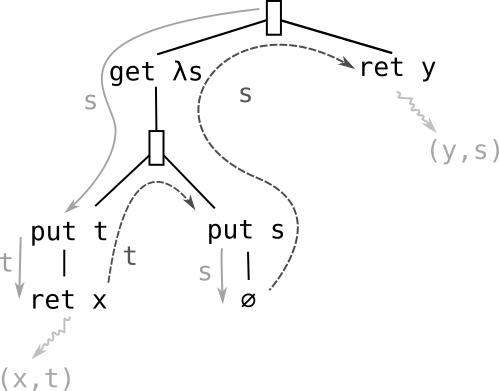
\includegraphics[scale=0.7]{sections/putR}
  \caption{Illustration of state-restoring put}
  \label{fig:putR}
\end{figure}

To help build understanding for \ensuremath{\Varid{put}_{\scaleobj{0.7}{\sf R}}}, Figure~\ref{fig:putR} shows the flow of
execution for the expression \ensuremath{(\Varid{put}_{\scaleobj{0.7}{\sf R}}\;\Varid{t}\mathbin{\hstretch{0.7}{>\!\!>}}\Varid{ret}\;\Varid{x})\mathbin{\talloblong}\Varid{ret}\;\Varid{y}}. Initially, the
state is \ensuremath{\Varid{s}}; it gets modified to \ensuremath{\Varid{t}} at the \ensuremath{\Varid{put}\;\Varid{t}} node after which the value
\ensuremath{\Varid{x}} is output with the working state \ensuremath{\Varid{t}}. Then, because we found a result, we
backtrack (since we're using global-state semantics, the state modification
caused by \ensuremath{\Varid{put}\;\Varid{t}} is not reversed), arriving in the \ensuremath{\Varid{side}} operation branch. The
\ensuremath{\Varid{put}\;\Varid{s}} operation is executed, which resets the state to \ensuremath{\Varid{s}}, and then the
branch immediately fails, so we backtrack to the right branch of the topmost
\ensuremath{(\talloblong)}. There the value \ensuremath{\Varid{y}} is output with working state \ensuremath{\Varid{s}}.

For some further intuition about \ensuremath{\Varid{put}_{\scaleobj{0.7}{\sf R}}}, consider \ensuremath{\Varid{put}_{\scaleobj{0.7}{\sf R}}\;\Varid{s}\mathbin{\hstretch{0.7}{>\!\!>}}\Varid{comp}} where \ensuremath{\Varid{comp}} is some arbitrary computation:
\begin{hscode}\SaveRestoreHook
\column{B}{@{}>{\hspre}l<{\hspost}@{}}%
\column{7}{@{}>{\hspre}l<{\hspost}@{}}%
\column{9}{@{}>{\hspre}l<{\hspost}@{}}%
\column{E}{@{}>{\hspre}l<{\hspost}@{}}%
\>[7]{}\Varid{put}_{\scaleobj{0.7}{\sf R}}\;\Varid{s}\mathbin{\hstretch{0.7}{>\!\!>}}\Varid{comp}{}\<[E]%
\\
\>[B]{}\mathbin{=}{}\<[7]%
\>[7]{}(\Varid{get}\mathrel{\hstretch{0.7}{>\!\!>\!\!=}}\lambda \Varid{s}_{0}\to \Varid{put}\;\Varid{s}\mathbin{\talloblong}\Varid{side}\;(\Varid{put}\;\Varid{s}_{0}))\mathbin{\hstretch{0.7}{>\!\!>}}\Varid{comp}{}\<[E]%
\\
\>[B]{}\mathbin{=}{}\<[9]%
\>[9]{}\mbox{\commentbegin  monad law, left-distributivity \eqref{eq:bind-mplus-dist}  \commentend}{}\<[E]%
\\
\>[B]{}\hsindent{7}{}\<[7]%
\>[7]{}\Varid{get}\mathrel{\hstretch{0.7}{>\!\!>\!\!=}}\lambda \Varid{s}_{0}\to (\Varid{put}\;\Varid{s}\mathbin{\hstretch{0.7}{>\!\!>}}\Varid{comp})\mathbin{\talloblong}(\Varid{side}\;(\Varid{put}\;\Varid{s}_{0})\mathbin{\hstretch{0.7}{>\!\!>}}\Varid{comp}){}\<[E]%
\\
\>[B]{}\mathbin{=}{}\<[9]%
\>[9]{}\mbox{\commentbegin  by \eqref{eq:bind-mzero-zero} \ensuremath{\Varid{\varnothing}\mathbin{\hstretch{0.7}{>\!\!>}}\Varid{comp}\mathrel{=}\Varid{\varnothing}}, monad laws  \commentend}{}\<[E]%
\\
\>[B]{}\hsindent{7}{}\<[7]%
\>[7]{}\Varid{get}\mathrel{\hstretch{0.7}{>\!\!>\!\!=}}\lambda \Varid{s}_{0}\to (\Varid{put}\;\Varid{s}\mathbin{\hstretch{0.7}{>\!\!>}}\Varid{comp})\mathbin{\talloblong}\Varid{side}\;(\Varid{put}\;\Varid{s}_{0})~~.{}\<[E]%
\ColumnHook
\end{hscode}\resethooks
Thanks to left-distributivity \eqref{eq:bind-mplus-dist}, \ensuremath{(\mathbin{\hstretch{0.7}{>\!\!>}}\Varid{comp})} is promoted into \ensuremath{(\talloblong)}.
Furthermore, the \ensuremath{(\mathbin{\hstretch{0.7}{>\!\!>}}\Varid{comp})} after \ensuremath{\Varid{side}\;(\Varid{put}\;\Varid{s}_{0})} is discarded by
\eqref{eq:bind-mzero-zero}.
In words, \ensuremath{\Varid{put}_{\scaleobj{0.7}{\sf R}}\;\Varid{s}\mathbin{\hstretch{0.7}{>\!\!>}}\Varid{comp}} saves the current state, computes \ensuremath{\Varid{comp}} using state \ensuremath{\Varid{s}}, and restores the saved state!
The subscript \ensuremath{\Conid{R}} stands for ``restore.''
Note also that \ensuremath{(\Varid{put}_{\scaleobj{0.7}{\sf R}}\;\Varid{s}\mathbin{\hstretch{0.7}{>\!\!>}}\Varid{m}_{1})\mathbin{\hstretch{0.7}{>\!\!>}}\Varid{m}_{2}\mathrel{=}\Varid{put}_{\scaleobj{0.7}{\sf R}}\;\Varid{s}\mathbin{\hstretch{0.7}{>\!\!>}}(\Varid{m}_{1}\mathbin{\hstretch{0.7}{>\!\!>}}\Varid{m}_{2})} --- the state restoration happens in the end.

The behaviour of \ensuremath{\Varid{put}_{\scaleobj{0.7}{\sf R}}} is rather tricky. It is instructive comparing
\begin{enumerate}[label=(\alph*)]
\item \ensuremath{\Varid{return}\;\Varid{x}},  \label{ex:putR-pitfalls-1}
\item \ensuremath{\Varid{put}\;\Varid{s}\mathbin{\hstretch{0.7}{>\!\!>}}\Varid{return}\;\Varid{x}}, \label{ex:putR-pitfalls-2}
\item \ensuremath{\Varid{put}_{\scaleobj{0.7}{\sf R}}\;\Varid{s}\mathbin{\hstretch{0.7}{>\!\!>}}\Varid{return}\;\Varid{x}}. \label{ex:putR-pitfalls-3}
\end{enumerate}
When run in initial state \ensuremath{\Varid{s}_{0}}, they all yield \ensuremath{\Varid{x}} as the result.
The final states after running \ref{ex:putR-pitfalls-1}, \ref{ex:putR-pitfalls-2} and \ref{ex:putR-pitfalls-3} are \ensuremath{\Varid{s}_{0}}, \ensuremath{\Varid{s}} and \ensuremath{\Varid{s}_{0}}, respectively.
However, \ref{ex:putR-pitfalls-3} does {\em not} behave identically to \ref{ex:putR-pitfalls-1} in all contexts!
For example, in the context \ensuremath{(\mathbin{\hstretch{0.7}{>\!\!>}}\Varid{get})}, we can tell them apart:
\ensuremath{\Varid{return}\;\Varid{x}\mathbin{\hstretch{0.7}{>\!\!>}}\Varid{get}} returns \ensuremath{\Varid{s}_{0}}, while \ensuremath{\Varid{put}_{\scaleobj{0.7}{\sf R}}\;\Varid{s}\mathbin{\hstretch{0.7}{>\!\!>}}\Varid{return}\;\Varid{x}\mathbin{\hstretch{0.7}{>\!\!>}}\Varid{get}} returns \ensuremath{\Varid{s}}, even though the program yields final state \ensuremath{\Varid{s}_{0}}.

We wish that \ensuremath{\Varid{put}_{\scaleobj{0.7}{\sf R}}}, when run with a global state, satisfies laws \eqref{eq:put-put} through \eqref{eq:mplus-bind-dist} ---
the state laws and the \emph{local} state laws.
If so, one could take a program written for a local state monad, replace all occurrences of \ensuremath{\Varid{put}} by \ensuremath{\Varid{put}_{\scaleobj{0.7}{\sf R}}}, and run the program with a global state.
Unfortunately this is not the case: \ensuremath{\Varid{put}_{\scaleobj{0.7}{\sf R}}} does satisfy {\bf put-put}~\eqref{eq:put-put} and {\bf put-get}~\eqref{eq:put-get}, but {\bf get-put}~\eqref{eq:get-put} fails ---
\ensuremath{\Varid{get}\mathrel{\hstretch{0.7}{>\!\!>\!\!=}}\Varid{put}_{\scaleobj{0.7}{\sf R}}} and \ensuremath{\Varid{return}\;()} can be
differentiated by some contexts, for example \ensuremath{(\mathbin{\hstretch{0.7}{>\!\!>}}\Varid{put}\;\Varid{t})}.
To see that, we calculate:
\begin{hscode}\SaveRestoreHook
\column{B}{@{}>{\hspre}l<{\hspost}@{}}%
\column{7}{@{}>{\hspre}l<{\hspost}@{}}%
\column{9}{@{}>{\hspre}l<{\hspost}@{}}%
\column{E}{@{}>{\hspre}l<{\hspost}@{}}%
\>[7]{}(\Varid{get}\mathrel{\hstretch{0.7}{>\!\!>\!\!=}}\Varid{put}_{\scaleobj{0.7}{\sf R}})\mathbin{\hstretch{0.7}{>\!\!>}}\Varid{put}\;\Varid{t}{}\<[E]%
\\
\>[B]{}\mathbin{=}{}\<[7]%
\>[7]{}(\Varid{get}\mathrel{\hstretch{0.7}{>\!\!>\!\!=}}\lambda \Varid{s}\to \Varid{get}\mathrel{\hstretch{0.7}{>\!\!>\!\!=}}\lambda \Varid{s}_{0}\to \Varid{put}\;\Varid{s}\mathbin{\talloblong}\Varid{side}\;(\Varid{put}\;\Varid{s}_{0}))\mathbin{\hstretch{0.7}{>\!\!>}}\Varid{put}\;\Varid{t}{}\<[E]%
\\
\>[B]{}\mathbin{=}{}\<[9]%
\>[9]{}\mbox{\commentbegin  {\bf get-get}  \commentend}{}\<[E]%
\\
\>[B]{}\hsindent{7}{}\<[7]%
\>[7]{}(\Varid{get}\mathrel{\hstretch{0.7}{>\!\!>\!\!=}}\lambda \Varid{s}\to \Varid{put}\;\Varid{s}\mathbin{\talloblong}\Varid{side}\;(\Varid{put}\;\Varid{s}))\mathbin{\hstretch{0.7}{>\!\!>}}\Varid{put}\;\Varid{t}{}\<[E]%
\\
\>[B]{}\mathbin{=}{}\<[9]%
\>[9]{}\mbox{\commentbegin  monad laws, left-distributivity  \commentend}{}\<[E]%
\\
\>[B]{}\hsindent{7}{}\<[7]%
\>[7]{}\Varid{get}\mathrel{\hstretch{0.7}{>\!\!>\!\!=}}\lambda \Varid{s}\to (\Varid{put}\;\Varid{s}\mathbin{\hstretch{0.7}{>\!\!>}}\Varid{put}\;\Varid{t})\mathbin{\talloblong}\Varid{side}\;(\Varid{put}\;\Varid{s}){}\<[E]%
\\
\>[B]{}\mathbin{=}{}\<[9]%
\>[9]{}\mbox{\commentbegin  {\bf put-put}  \commentend}{}\<[E]%
\\
\>[B]{}\hsindent{7}{}\<[7]%
\>[7]{}\Varid{get}\mathrel{\hstretch{0.7}{>\!\!>\!\!=}}\lambda \Varid{s}\to \Varid{put}\;\Varid{t}\mathbin{\talloblong}\Varid{side}\;(\Varid{put}\;\Varid{s})~~.{}\<[E]%
\ColumnHook
\end{hscode}\resethooks
Meanwhile, \ensuremath{\Varid{return}\;()\mathbin{\hstretch{0.7}{>\!\!>}}\Varid{put}\;\Varid{t}\mathrel{=}\Varid{put}\;\Varid{t}}, which does not behave in the same way as \ensuremath{\Varid{get}\mathrel{\hstretch{0.7}{>\!\!>\!\!=}}\lambda \Varid{s}\to \Varid{put}\;\Varid{t}\mathbin{\talloblong}\Varid{side}\;(\Varid{put}\;\Varid{s})} when $s \neq t$.

In a global-state setting, the left-distributivity law
\eqref{eq:bind-mplus-dist} makes it tricky to reason about combinations of
\ensuremath{(\talloblong)} and \ensuremath{(\mathrel{\hstretch{0.7}{>\!\!>\!\!=}})} operators. Suppose we have a program \ensuremath{(\Varid{m}\mathbin{\talloblong}\Varid{n})}, and we
construct an extended program by binding a continuation \ensuremath{\Varid{f}} to it such that we
get \ensuremath{(\Varid{m}\mathbin{\talloblong}\Varid{n})\mathrel{\hstretch{0.7}{>\!\!>\!\!=}}\Varid{f}} (where \ensuremath{\Varid{f}} might modify the state). Under global-state
semantics, the evaluation of the right branch is influenced by the state
modifications performed by evaluating the left branch. So by
\eqref{eq:bind-mplus-dist}, this means that when we get to evaluating the \ensuremath{\Varid{n}}
subprogram in the extended program, it will do so with a different initial state
(the one obtained after running \ensuremath{\Varid{m}\mathrel{\hstretch{0.7}{>\!\!>\!\!=}}\Varid{f}}) compared to the initial state in the
original program (the one obtained by running \ensuremath{\Varid{m}}). In other words, placing our
program in a different context changed the meaning of one of its subprograms. So
it is difficult to reason about programs compositionally in this
setting---some properties hold only when we take the entire program into
consideration.

It turns out that all properties we need do hold, provided that {\em all}
occurrences of \ensuremath{\Varid{put}} are replaced by \ensuremath{\Varid{put}_{\scaleobj{0.7}{\sf R}}}---problematic contexts such as
\ensuremath{\Varid{put}\;\Varid{t}} above are thus ruled out. However, that ``all \ensuremath{\Varid{put}} are replaced by
\ensuremath{\Varid{put}_{\scaleobj{0.7}{\sf R}}}'' is a global property, and to properly talk about it we have to formally
define contexts, which is what we will do in Section~\ref{sec:ctxt-trans}.
Notice though, that simulation of local state semantics by judicious use of
\ensuremath{\Varid{put}_{\scaleobj{0.7}{\sf R}}} does not avoid the unnecessary copying mentioned in
Section~\ref{sec:space-usage}, it merely makes it explicit in the program.
We will address this shortcoming in Section~\ref{sec:backtrack-gs}.
\section{Proving the $\mathit{put}_{\text{R}}$ Transformation Correct For a Given Implementation}
Before we tackle the general proof of correctness of the \ensuremath{\Varid{put}_{\scaleobj{0.7}{\sf R}}} transformation
correct, we dip our toes into something a bit more straightforward: showing that
the transformation is correct for specific implementations of global and local
state. This lets us use a somewhat more concrete setting to introduce some
infrastructure needed for the more general proof, as well as demonstrate a case
study of a fold fusion proof (TODO: citation), an elegant and powerful technique
that is interesting in its own right.

In the previous sections we have been mixing syntax and semantics,
which we avoid in this section by defining the program syntax as a free monad
(TODO: citation).
This way we avoid the need for a type-level distinction between programs
with local-state semantics and programs with global-state semantics.
\begin{hscode}\SaveRestoreHook
\column{B}{@{}>{\hspre}l<{\hspost}@{}}%
\column{3}{@{}>{\hspre}l<{\hspost}@{}}%
\column{7}{@{}>{\hspre}l<{\hspost}@{}}%
\column{11}{@{}>{\hspre}l<{\hspost}@{}}%
\column{15}{@{}>{\hspre}l<{\hspost}@{}}%
\column{24}{@{}>{\hspre}l<{\hspost}@{}}%
\column{E}{@{}>{\hspre}l<{\hspost}@{}}%
\>[B]{}\mathbf{data}\;\Conid{Free}\;\Varid{f}\;\Varid{a}\;\mathbf{where}{}\<[E]%
\\
\>[B]{}\hsindent{3}{}\<[3]%
\>[3]{}\Conid{Ret}\mathbin{::}\Varid{a}{}\<[24]%
\>[24]{}\to \Conid{Free}\;\Varid{f}\;\Varid{a}{}\<[E]%
\\
\>[B]{}\hsindent{3}{}\<[3]%
\>[3]{}\Conid{Op}{}\<[7]%
\>[7]{}\mathbin{::}\Varid{f}\;(\Conid{Free}\;\Varid{f}\;\Varid{a}){}\<[24]%
\>[24]{}\to \Conid{Free}\;\Varid{f}\;\Varid{a}{}\<[E]%
\\[\blanklineskip]%
\>[B]{}\mathbf{instance}\;\Conid{Functor}\;\Varid{f}\Rightarrow \Conid{Functor}\;(\Conid{Free}\;\Varid{f})\;\mathbf{where}{}\<[E]%
\\
\>[B]{}\hsindent{3}{}\<[3]%
\>[3]{}\Varid{fmap}\;\Varid{f}\;(\Conid{Ret}\;\Varid{x})\mathrel{=}\Conid{Ret}\;(\Varid{f}\;\Varid{x}){}\<[E]%
\\
\>[B]{}\hsindent{3}{}\<[3]%
\>[3]{}\Varid{fmap}\;\Varid{f}\;(\Conid{Op}\;{}\<[15]%
\>[15]{}\Varid{o})\mathrel{=}\Conid{Op}\;(\Varid{fmap}\;(\Varid{fmap}\;\Varid{f})\;\Varid{o}){}\<[E]%
\\[\blanklineskip]%
\>[B]{}\mathbf{instance}\;\Conid{Functor}\;\Varid{f}\Rightarrow \Conid{Monad}\;(\Conid{Free}\;\Varid{f})\;\mathbf{where}{}\<[E]%
\\
\>[B]{}\hsindent{3}{}\<[3]%
\>[3]{}\Varid{return}{}\<[11]%
\>[11]{}\mathrel{=}\Varid{pure}{}\<[E]%
\\
\>[B]{}\hsindent{3}{}\<[3]%
\>[3]{}\Conid{Ret}\;\Varid{x}\mathrel{\hstretch{0.7}{>\!\!>\!\!=}}\Varid{g}\mathrel{=}\Varid{g}\;\Varid{x}{}\<[E]%
\\
\>[B]{}\hsindent{3}{}\<[3]%
\>[3]{}\Conid{Op}\;\Varid{op}\mathrel{\hstretch{0.7}{>\!\!>\!\!=}}\Varid{g}\mathrel{=}\Conid{Op}\;(\Varid{fmap}\;(\mathrel{\hstretch{0.7}{>\!\!>\!\!=}}\Varid{g})\;\Varid{op}){}\<[E]%
\ColumnHook
\end{hscode}\resethooks
The state and nondeterminism interfaces are provided as ``algebras''. These are
functors equipped with a constructor for each operation they support.
\begin{hscode}\SaveRestoreHook
\column{B}{@{}>{\hspre}l<{\hspost}@{}}%
\column{3}{@{}>{\hspre}l<{\hspost}@{}}%
\column{5}{@{}>{\hspre}l<{\hspost}@{}}%
\column{12}{@{}>{\hspre}l<{\hspost}@{}}%
\column{25}{@{}>{\hspre}l<{\hspost}@{}}%
\column{E}{@{}>{\hspre}l<{\hspost}@{}}%
\>[3]{}\mathbf{data}\;\Conid{StateF}\;\Varid{a}\;\mathbf{where}{}\<[E]%
\\
\>[3]{}\hsindent{2}{}\<[5]%
\>[5]{}\Conid{Get}{}\<[12]%
\>[12]{}\mathbin{::}(\Conid{S}\to \Varid{a}){}\<[25]%
\>[25]{}\to \Conid{StateF}\;\Varid{a}{}\<[E]%
\\
\>[3]{}\hsindent{2}{}\<[5]%
\>[5]{}\Conid{Put}{}\<[12]%
\>[12]{}\mathbin{::}\Conid{S}\to \Varid{a}{}\<[25]%
\>[25]{}\to \Conid{StateF}\;\Varid{a}{}\<[E]%
\\
\>[3]{}\hsindent{2}{}\<[5]%
\>[5]{}\mathbf{deriving}\;\Conid{Functor}{}\<[E]%
\\[\blanklineskip]%
\>[3]{}\mathbf{data}\;\Conid{NondetF}\;\Varid{a}\;\mathbf{where}{}\<[E]%
\\
\>[3]{}\hsindent{2}{}\<[5]%
\>[5]{}\Varid{\varnothing}{}\<[12]%
\>[12]{}\mathbin{::}\Conid{NondetF}\;\Varid{a}{}\<[E]%
\\
\>[3]{}\hsindent{2}{}\<[5]%
\>[5]{}(\talloblong){}\<[12]%
\>[12]{}\mathbin{::}\Varid{a}\to \Varid{a}\to \Conid{NondetF}\;\Varid{a}{}\<[E]%
\\
\>[3]{}\hsindent{2}{}\<[5]%
\>[5]{}\mathbf{deriving}\;\Conid{Functor}{}\<[E]%
\ColumnHook
\end{hscode}\resethooks
In this encoding, the type \ensuremath{\Conid{Free}\;\Conid{StateF}\;\Varid{a}} represents stateful computations, and
similarly the type \ensuremath{\Conid{Free}\;\Conid{NondetF}\;\Varid{a}} represents nondeterministic computations.
Note that in this representation, our programs are written in a
continuation-passing style. For instance, where in the previous section we would
have written \ensuremath{\Varid{put}\;\Varid{t}\mathbin{\hstretch{0.7}{>\!\!>}}\Varid{get}}, we now write \ensuremath{\Conid{Op}\;(\Conid{Put}\;\Varid{t}\;(\Conid{Op}\;\Conid{Get}))}.
Computations with multiple effects can be typed with a sum type \ensuremath{(\mathbin{+})} over types
of kind \ensuremath{\mathbin{*}\to \mathbin{*}}.
\begin{hscode}\SaveRestoreHook
\column{B}{@{}>{\hspre}l<{\hspost}@{}}%
\column{3}{@{}>{\hspre}l<{\hspost}@{}}%
\column{5}{@{}>{\hspre}l<{\hspost}@{}}%
\column{E}{@{}>{\hspre}l<{\hspost}@{}}%
\>[3]{}\mathbf{data}\;(\Varid{f}\mathbin{+}\Varid{g})\;\Varid{a}\;\mathbf{where}{}\<[E]%
\\
\>[3]{}\hsindent{2}{}\<[5]%
\>[5]{}\Conid{Inl}\mathbin{::}\Varid{f}\;\Varid{a}\to (\Varid{f}\mathbin{+}\Varid{g})\;\Varid{a}{}\<[E]%
\\
\>[3]{}\hsindent{2}{}\<[5]%
\>[5]{}\Conid{Inr}\mathbin{::}\Varid{g}\;\Varid{a}\to (\Varid{f}\mathbin{+}\Varid{g})\;\Varid{a}{}\<[E]%
\\
\>[3]{}\hsindent{2}{}\<[5]%
\>[5]{}\mathbf{deriving}\;\Conid{Functor}{}\<[E]%
\ColumnHook
\end{hscode}\resethooks
The type \ensuremath{\Conid{Free}\;(\Conid{NondetF}\mathbin{+}\Conid{StateF})\;\Varid{a}} is one way to encode programs which have
both nondeterminism and state as effects. So is \ensuremath{\Conid{Free}\;(\Conid{StateF}\mathbin{+}\Conid{NondetF})\;\Varid{a}}, or
more generally \ensuremath{\Conid{Functor}\;\Varid{f}\Rightarrow \Conid{Free}\;(\Conid{StateF}\mathbin{+}(\Conid{NondetF}\mathbin{+}\Varid{f}))\;\Varid{a}} (where \ensuremath{\Varid{f}} may
introduce additional effects). 
Where in the previous section we would have written \ensuremath{\Varid{put}\;\Varid{t}\mathbin{\hstretch{0.7}{>\!\!>}}\Varid{\varnothing}}, we now
write \ensuremath{\Conid{Op}\;(\Conid{Inr}\;(\Conid{Put}\;\Varid{t}\;(\Conid{Op}\;(\Conid{Inl}\;\Varid{\varnothing}))))\mathbin{::}\Conid{Free}\;(\Conid{NondetF}\mathbin{+}\Conid{StateF})\;\Varid{a}}. We will
later introduce notation to make our syntax a bit less noisy.
The \ensuremath{(\mathbin{+})} type is morally commutative, associative, and has a zero element:
\begin{hscode}\SaveRestoreHook
\column{B}{@{}>{\hspre}l<{\hspost}@{}}%
\column{9}{@{}>{\hspre}l<{\hspost}@{}}%
\column{E}{@{}>{\hspre}l<{\hspost}@{}}%
\>[B]{}\Varid{comm}{}\<[9]%
\>[9]{}\mathbin{::}(\Conid{Functor}\;\Varid{f},\Conid{Functor}\;\Varid{g})\Rightarrow \Conid{Free}\;(\Varid{f}\mathbin{+}\Varid{g})\;\Varid{a}\to \Conid{Free}\;(\Varid{g}\mathbin{+}\Varid{f})\;\Varid{a}{}\<[E]%
\\
\>[B]{}\Varid{assocl}{}\<[9]%
\>[9]{}\mathbin{::}(\Conid{Functor}\;\Varid{f},\Conid{Functor}\;\Varid{g},\Conid{Functor}\;\Varid{h}){}\<[E]%
\\
\>[9]{}\Rightarrow \Conid{Free}\;(\Varid{f}\mathbin{+}(\Varid{g}\mathbin{+}\Varid{h}))\;\Varid{a}\to \Conid{Free}\;((\Varid{f}\mathbin{+}\Varid{g})\mathbin{+}\Varid{h})\;\Varid{a}{}\<[E]%
\\
\>[B]{}\Varid{assocr}{}\<[9]%
\>[9]{}\mathbin{::}(\Conid{Functor}\;\Varid{f},\Conid{Functor}\;\Varid{g},\Conid{Functor}\;\Varid{h}){}\<[E]%
\\
\>[9]{}\Rightarrow \Conid{Free}\;((\Varid{f}\mathbin{+}\Varid{g})\mathbin{+}\Varid{h})\;\Varid{a}\to \Conid{Free}\;(\Varid{f}\mathbin{+}(\Varid{g}\mathbin{+}\Varid{h}))\;\Varid{a}{}\<[E]%
\\[\blanklineskip]%
\>[B]{}\mathbf{data}\;\Conid{Nil}\;\Varid{a}\;\mathbf{deriving}\;\Conid{Functor}{}\<[E]%
\\[\blanklineskip]%
\>[B]{}\Varid{hNil}{}\<[9]%
\>[9]{}\mathbin{::}\Conid{Free}\;\Conid{Nil}\;\Varid{a}\to \Varid{a}{}\<[E]%
\\
\>[B]{}\Varid{hNil}\;(\Conid{Ret}\;\Varid{x})\mathrel{=}\Varid{x}{}\<[E]%
\\
\>[B]{}\mbox{\onelinecomment  other cases cannot occur}{}\<[E]%
\ColumnHook
\end{hscode}\resethooks
This zero element is an empty ``effect set'': a program of type \ensuremath{\Conid{Free}\;\Conid{Nil}\;\Varid{a}}
represents a program that computes an \ensuremath{\Varid{a}} without relying on any effects (this
type is commutative with just the type \ensuremath{\Varid{a}}).

With the \ensuremath{\Conid{Free}}-based encoding we can not only write programs
with effect sets composed from smaller effect sets, we can also write the {\em
handlers} for these effect sets compositionally.
For state and nondeterminism, we respectively write the following types for
their ``compositional'' handlers:
\begin{hscode}\SaveRestoreHook
\column{B}{@{}>{\hspre}l<{\hspost}@{}}%
\column{10}{@{}>{\hspre}l<{\hspost}@{}}%
\column{41}{@{}>{\hspre}l<{\hspost}@{}}%
\column{E}{@{}>{\hspre}l<{\hspost}@{}}%
\>[B]{}\Varid{hState}{}\<[10]%
\>[10]{}\mathbin{::}\Conid{Functor}\;\Varid{f}\Rightarrow \Conid{Free}\;(\Conid{StateF}{}\<[41]%
\>[41]{}\mathbin{+}\Varid{f})\;\Varid{a}\to (\Conid{S}\to \Conid{Free}\;\Varid{f}\;(\Varid{a},\Conid{S})){}\<[E]%
\\
\>[B]{}\Varid{hNondet}{}\<[10]%
\>[10]{}\mathbin{::}\Conid{Functor}\;\Varid{f}\Rightarrow \Conid{Free}\;(\Conid{NondetF}{}\<[41]%
\>[41]{}\mathbin{+}\Varid{f})\;\Varid{a}\to \Conid{Free}\;\Varid{f}\;(\Conid{Bag}\;\Varid{a}){}\<[E]%
\ColumnHook
\end{hscode}\resethooks
Here the \ensuremath{\Conid{Bag}} type represents a multiset data structure. We give a simple
example implementation:
\begin{hscode}\SaveRestoreHook
\column{B}{@{}>{\hspre}l<{\hspost}@{}}%
\column{3}{@{}>{\hspre}l<{\hspost}@{}}%
\column{31}{@{}>{\hspre}l<{\hspost}@{}}%
\column{53}{@{}>{\hspre}l<{\hspost}@{}}%
\column{E}{@{}>{\hspre}l<{\hspost}@{}}%
\>[3]{}\mathbf{newtype}\;\Conid{Bag}\;\Varid{a}\mathrel{=}\Conid{Bag}\;[\mskip1.5mu \Varid{a}\mskip1.5mu]\;\mathbf{deriving}\;\Conid{Functor}{}\<[E]%
\\[\blanklineskip]%
\>[3]{}\mathbf{instance}\;\Conid{Semigroup}\;(\Conid{Bag}\;\Varid{a})\;{}\<[31]%
\>[31]{}\mathbf{where}\;\Conid{Bag}\;\Varid{l}\mathbin{\Diamond}\Conid{Bag}\;\Varid{r}{}\<[53]%
\>[53]{}\mathrel{=}\Conid{Bag}\;(\Varid{l}\mathbin{+\!\!\!\!\!+}\Varid{r}){}\<[E]%
\\[\blanklineskip]%
\>[3]{}\mathbf{instance}\;\Conid{Monoid}\;(\Conid{Bag}\;\Varid{a})\;{}\<[31]%
\>[31]{}\mathbf{where}\;\Varid{mempty}{}\<[53]%
\>[53]{}\mathrel{=}\Conid{Bag}\;[\mskip1.5mu \mskip1.5mu]{}\<[E]%
\\[\blanklineskip]%
\>[3]{}\mathbf{instance}\;\Conid{Eq}\;(\Conid{Bag}\;\Varid{a})\;{}\<[31]%
\>[31]{}\mathbf{where}\;\Conid{Bag}\;\Varid{l}\doubleequals\Conid{Bag}\;\Varid{r}{}\<[53]%
\>[53]{}\mathrel{=}\Varid{sort}\;\Varid{l}\doubleequals\Varid{sort}\;\Varid{r}{}\<[E]%
\\[\blanklineskip]%
\>[3]{}\Varid{singleton}\mathbin{::}\Varid{a}\to \Conid{Bag}\;\Varid{a}{}\<[E]%
\\
\>[3]{}\Varid{singleton}\;\Varid{x}\mathrel{=}\Conid{Bag}\;[\mskip1.5mu \Varid{x}\mskip1.5mu]{}\<[E]%
\\[\blanklineskip]%
\>[3]{}\Varid{elem}\mathbin{::}\Conid{Eq}\;\Varid{a}\Rightarrow \Varid{a}\to \Conid{Bag}\;\Varid{a}\to \Conid{Int}{}\<[E]%
\\
\>[3]{}\Varid{elem}\;\Varid{x}\;(\Conid{Bag}\;\Varid{xs})\mathrel{=}\Varid{length}\;(\Varid{filter}\;(\doubleequals\Varid{x})\;\Varid{xs}){}\<[E]%
\\[\blanklineskip]%
\>[3]{}\Varid{bagFlatten}\mathbin{::}\Conid{Bag}\;(\Conid{Bag}\;\Varid{a})\to \Conid{Bag}\;\Varid{a}{}\<[E]%
\\
\>[3]{}\Varid{bagFlatten}\;(\Conid{Bag}\;\Varid{bags})\mathrel{=}\Conid{Bag}\;(\Varid{concat}\;\Varid{bags}){}\<[E]%
\ColumnHook
\end{hscode}\resethooks
The type of the \ensuremath{\Varid{hState}} and \ensuremath{\Varid{hNondet}} handlers indicate that they handle one
effect of the effect set of the program, yielding a new effectful program where
the effect set contains all the remaining effects.  This is a bit reminiscent
of a ``linked list'' of effects. Like a linked list, a ``nil'' element is
needed to terminate the list; this is provided to us by the \ensuremath{\Conid{Nil}} type.

For instance, we can compose a handler \ensuremath{\Varid{hLocal}} for local state semantics out of
the ``atomic'' handlers for state and nondeterminism.
We will only be interested in the results of the computation, not the final
states, so the final step of our local state handler is to throw away the state
information (with \ensuremath{\Varid{fmap}\;\Varid{fst}}).
\begin{hscode}\SaveRestoreHook
\column{B}{@{}>{\hspre}l<{\hspost}@{}}%
\column{10}{@{}>{\hspre}l<{\hspost}@{}}%
\column{E}{@{}>{\hspre}l<{\hspost}@{}}%
\>[B]{}\Varid{hLocal'}{}\<[10]%
\>[10]{}\mathbin{::}\Conid{Free}\;(\Conid{StateF}\mathbin{+}(\Conid{NondetF}\mathbin{+}\Conid{Nil}))\;\Varid{a}\to (\Conid{S}\to \Conid{Bag}\;(\Varid{a},\Conid{S})){}\<[E]%
\\
\>[B]{}\Varid{hLocal'}{}\<[10]%
\>[10]{}\mathrel{=}\Varid{fmap}\;(\Varid{hNil}\mathbin{\cdot}\Varid{hNondet})\mathbin{\cdot}\Varid{hState}{}\<[E]%
\\[\blanklineskip]%
\>[B]{}\Varid{hLocal}{}\<[10]%
\>[10]{}\mathbin{::}\Conid{Free}\;(\Conid{StateF}\mathbin{+}(\Conid{NondetF}\mathbin{+}\Conid{Nil}))\;\Varid{a}\to (\Conid{S}\to \Conid{Bag}\;\Varid{a}){}\<[E]%
\\
\>[B]{}\Varid{hLocal}{}\<[10]%
\>[10]{}\mathrel{=}\Varid{fmap}\;(\Varid{fmap}\;\Varid{fst})\mathbin{\cdot}\Varid{hLocal'}{}\<[E]%
\ColumnHook
\end{hscode}\resethooks
In other words, local state semantics is the semantics where we
nondeterministically choose between different stateful computations. This
matches our intuition of local state semantics: if we can picture stateful,
nondeterministic programs as trees, then local state semantics is the
interpretation of the tree where each result of the (nondeterministic, stateful)
computation corresponds to a path from root to leaf in the tree. One can compute
each of these paths entirely independently from the other paths. 
Later on, we shall prove that this composition forms a valid
implementation of local state semantics.

Global state semantics can be implemented by simply inverting the order of the
handlers: rather than nondeterministically choosing between stateful
computations as local state does, in global state semantics we'll run a
single state through a nondeterministic computation.
Just like with the local state handler, we are not interested in the final state
of the computation, only in the results, so the final step of our handler is a
\ensuremath{\Varid{fmap}\;\Varid{fst}}.
\begin{hscode}\SaveRestoreHook
\column{B}{@{}>{\hspre}l<{\hspost}@{}}%
\column{11}{@{}>{\hspre}l<{\hspost}@{}}%
\column{E}{@{}>{\hspre}l<{\hspost}@{}}%
\>[B]{}\Varid{hGlobal'}{}\<[11]%
\>[11]{}\mathbin{::}\Conid{Free}\;(\Conid{NondetF}\mathbin{+}(\Conid{StateF}\mathbin{+}\Conid{Nil}))\;\Varid{a}\to (\Conid{S}\to (\Conid{Bag}\;\Varid{a},\Conid{S})){}\<[E]%
\\
\>[B]{}\Varid{hGlobal'}{}\<[11]%
\>[11]{}\mathrel{=}\Varid{fmap}\;\Varid{hNil}\mathbin{\cdot}\Varid{hState}\mathbin{\cdot}\Varid{hNondet}{}\<[E]%
\\[\blanklineskip]%
\>[B]{}\Varid{hGlobal}{}\<[11]%
\>[11]{}\mathbin{::}\Conid{Free}\;(\Conid{NondetF}\mathbin{+}(\Conid{StateF}\mathbin{+}\Conid{Nil}))\;\Varid{a}\to (\Conid{S}\to \Conid{Bag}\;\Varid{a}){}\<[E]%
\\
\>[B]{}\Varid{hGlobal}{}\<[11]%
\>[11]{}\mathrel{=}\Varid{fmap}\;\Varid{fst}\mathbin{\cdot}\Varid{hGlobal'}{}\<[E]%
\ColumnHook
\end{hscode}\resethooks
We argue the correctness of \ensuremath{\Varid{hLocal}} and \ensuremath{\Varid{hGlobal}} (with respect to laws of
respectively local and global state semantics) in~\ref{sec:correctness-handlers}.

%From this point onwards, we will omit some technical details where confusion is
%unlikely to arise. In particular, we will omit the |Op|, |Inl| and |Inr|
%constructors from our programs. For example, when we should write
%|Op (Inl (Get (\x -> Op (Inr (p x `mplus` q x)))))| (an instance of the type
%|Free (StateF + NondetF) a|), we shall instead write
%|Get (\x -> p x `mplus` q x)|, and by this actually mean an element of the type
%|Free (StateF + NondetF) a| instead of the type |StateF (NondetF a)|.
%Moreover, in our notation the same term is also an instance of
%|Free (NondetF + StateF) a|, and of |Free| 

\subsection{Folds and Fold Fusion}
\label{sec:fold-fusion}
(TODO citations)
Rather than defining our handlers directly by writing a general recursive
function, we will write them as folds, a type of structural recursion.
\begin{hscode}\SaveRestoreHook
\column{B}{@{}>{\hspre}l<{\hspost}@{}}%
\column{3}{@{}>{\hspre}l<{\hspost}@{}}%
\column{25}{@{}>{\hspre}l<{\hspost}@{}}%
\column{E}{@{}>{\hspre}l<{\hspost}@{}}%
\>[3]{}\Varid{fold}\mathbin{::}\Conid{Functor}\;\Varid{f}\Rightarrow (\Varid{a}\to \Varid{r})\to (\Varid{f}\;\Varid{r}\to \Varid{r})\to \Conid{Free}\;\Varid{f}\;\Varid{r}\to \Varid{r}{}\<[E]%
\\
\>[3]{}\Varid{fold}\;\Varid{gen}\;\Varid{alg}\;(\Conid{Ret}\;\Varid{x}){}\<[25]%
\>[25]{}\mathrel{=}\Varid{gen}\;\Varid{x}{}\<[E]%
\\
\>[3]{}\Varid{fold}\;\Varid{gen}\;\Varid{alg}\;(\Conid{Op}\;\Varid{op}){}\<[25]%
\>[25]{}\mathrel{=}\Varid{alg}\;(\Varid{fmap}\;(\Varid{fold}\;\Varid{gen}\;\Varid{alg})\;\Varid{op}){}\<[E]%
\ColumnHook
\end{hscode}\resethooks
This more principled approach gives us more leverage when reasoning about our
programs, as certain laws hold for programs defined through fusion.
In particular, we are interested in the {\em fold fusion} law:
\begin{align*}
  \ensuremath{\Varid{h}\mathbin{\cdot}\Varid{fold}\;\Varid{gen}\;\Varid{alg}} & = \ensuremath{\Varid{fold}\;\Varid{gen'}\;\Varid{alg'}} \\
                     & \Uparrow \\
  \ensuremath{\Varid{h}\mathbin{\cdot}\Varid{gen}}          & = \ensuremath{\Varid{gen'}} \\
  \ensuremath{\Varid{h}\mathbin{\cdot}\Varid{alg}}          & = \ensuremath{\Varid{alg'}\mathbin{\cdot}\Varid{fmap}\;\Varid{h}}
\end{align*}
Informally, this law states that a post-processing step (\ensuremath{\Varid{h}}) following a fold
can, if certain conditions are met, be {\em fused} into the fold.
Moreover, it will soon become apparent that the fold fusion law is not only
helpful in proving two known programs equivalent, but in fact it can often help
in finding a fused program given a composition of two programs. This discovered
program will then be correct by construction.

We can define the state and nondeterminism handlers as folds.
\begin{hscode}\SaveRestoreHook
\column{B}{@{}>{\hspre}l<{\hspost}@{}}%
\column{3}{@{}>{\hspre}l<{\hspost}@{}}%
\column{5}{@{}>{\hspre}l<{\hspost}@{}}%
\column{32}{@{}>{\hspre}l<{\hspost}@{}}%
\column{37}{@{}>{\hspre}l<{\hspost}@{}}%
\column{E}{@{}>{\hspre}l<{\hspost}@{}}%
\>[B]{}\Varid{hState}\mathbin{::}\Conid{Functor}\;\Varid{f}\Rightarrow \Conid{Free}\;(\Conid{StateF}\mathbin{+}\Varid{f})\;\Varid{a}\to (\Conid{S}\to \Conid{Free}\;\Varid{f}\;(\Varid{a},\Conid{S})){}\<[E]%
\\
\>[B]{}\Varid{hState}\mathrel{=}\Varid{fold}\;\Varid{genState}\;\Varid{algState}{}\<[E]%
\\
\>[B]{}\hsindent{3}{}\<[3]%
\>[3]{}\mathbf{where}{}\<[E]%
\\
\>[3]{}\hsindent{2}{}\<[5]%
\>[5]{}\Varid{genState}\;\Varid{x}{}\<[32]%
\>[32]{}\mathrel{=}\lambda \Varid{s}\to \Conid{Ret}\;(\Varid{x},\Varid{s}){}\<[E]%
\\
\>[3]{}\hsindent{2}{}\<[5]%
\>[5]{}\Varid{algState}\;(\Conid{Inl}\;(\Conid{Get}\;\Varid{k})){}\<[32]%
\>[32]{}\mathrel{=}\lambda \Varid{s}\to \Varid{k}\;\Varid{s}\;\Varid{s}{}\<[E]%
\\
\>[3]{}\hsindent{2}{}\<[5]%
\>[5]{}\Varid{algState}\;(\Conid{Inl}\;(\Conid{Put}\;\Varid{t}\;\Varid{k})){}\<[32]%
\>[32]{}\mathrel{=}\lambda \anonymous \to \Varid{k}\;\Varid{t}{}\<[E]%
\\
\>[3]{}\hsindent{2}{}\<[5]%
\>[5]{}\Varid{algState}\;(\Conid{Inr}\;\Varid{p}){}\<[32]%
\>[32]{}\mathrel{=}\lambda \Varid{s}\to \Conid{Op}\;(\Varid{fmap}\;(\mathbin{\$}\Varid{s})\;\Varid{p}){}\<[E]%
\\[\blanklineskip]%
\>[B]{}\Varid{hNondet}\mathbin{::}\Conid{Functor}\;\Varid{f}\Rightarrow \Conid{Free}\;(\Conid{NondetF}\mathbin{+}\Varid{f})\;\Varid{a}\to \Conid{Free}\;\Varid{f}\;(\Conid{Bag}\;\Varid{a}){}\<[E]%
\\
\>[B]{}\Varid{hNondet}\mathrel{=}\Varid{fold}\;\Varid{genNondet}\;\Varid{algNondet}{}\<[E]%
\\
\>[B]{}\hsindent{3}{}\<[3]%
\>[3]{}\mathbf{where}{}\<[E]%
\\
\>[3]{}\hsindent{2}{}\<[5]%
\>[5]{}\Varid{genNondet}\;\Varid{x}{}\<[37]%
\>[37]{}\mathrel{=}\Conid{Ret}\;(\Varid{singleton}\;\Varid{x}){}\<[E]%
\\
\>[3]{}\hsindent{2}{}\<[5]%
\>[5]{}\Varid{algNondet}\;(\Conid{Inl}\;\Varid{\varnothing}){}\<[37]%
\>[37]{}\mathrel{=}\Conid{Ret}\;\Varid{mempty}{}\<[E]%
\\
\>[3]{}\hsindent{2}{}\<[5]%
\>[5]{}\Varid{algNondet}\;(\Conid{Inl}\;(\Varid{p}\mathbin{\talloblong}\Varid{q})){}\<[37]%
\>[37]{}\mathrel{=}(\mathbin{\Diamond})\mathrel{\raisebox{0.5\depth}{\scaleobj{0.5}{\langle}} \scaleobj{0.8}{\$} \raisebox{0.5\depth}{\scaleobj{0.5}{\rangle}}}\Varid{p}\mathrel{\raisebox{0.5\depth}{\scaleobj{0.5}{\langle}} \scaleobj{0.8}{\ast} \raisebox{0.5\depth}{\scaleobj{0.5}{\rangle}}}\Varid{q}{}\<[E]%
\\
\>[3]{}\hsindent{2}{}\<[5]%
\>[5]{}\Varid{algNondet}\;(\Conid{Inr}\;\Varid{op}){}\<[37]%
\>[37]{}\mathrel{=}\Conid{Op}\;\Varid{op}{}\<[E]%
\ColumnHook
\end{hscode}\resethooks
With our atomic handlers defined, we have also gained complete definitions for
\ensuremath{\Varid{hLocal}} and \ensuremath{\Varid{hGlobal}}, as we know how to compose them from the atomic
handlers. 

\subsubsection{A Note on Notation}
Before moving on, we will attempt to simplify our notation a bit, as it is
already becoming apparent that it's getting cumbersome, and this will
only get worse as we start reasoning with it.  For example, to write a ``get''
operator in a program typed with \ensuremath{\Conid{Free}\;(\Conid{NondetF}\mathbin{+}(\Conid{StateF}\mathbin{+}\Conid{NilF}))\;\Varid{a}} requires
us to write \ensuremath{\Conid{Inr}\;(\Conid{Inl}\;(\Conid{Op}\;(\Conid{Get}\;\Varid{k})))}. Even worse,
although we see the types 
\ensuremath{\Conid{Free}\;(\Conid{NondetF}\mathbin{+}(\Conid{StateF}\mathbin{+}\Conid{NilF}))\;\Varid{a}} and \ensuremath{\Conid{Free}\;(\Conid{StateF}\mathbin{+}(\Conid{NondetF}\mathbin{+}\Conid{NilF}))\;\Varid{a}} as
morally the same, to convert a value of one of them into the other requires some
tedious type gymnastics.
For instance, if we want \ensuremath{\Varid{hGlobal}} to operate on the same
type of programs as \ensuremath{\Varid{hLocal}}, we need to perform some intermediate transformations:
\begin{hscode}\SaveRestoreHook
\column{B}{@{}>{\hspre}l<{\hspost}@{}}%
\column{E}{@{}>{\hspre}l<{\hspost}@{}}%
\>[B]{}\Varid{hGlobal'}\mathbin{::}\Conid{Free}\;(\Conid{StateF}\mathbin{+}(\Conid{NondetF}\mathbin{+}\Conid{Nil}))\;\Varid{a}\to (\Conid{S}\to (\Conid{Bag}\;\Varid{a},\Conid{S})){}\<[E]%
\\
\>[B]{}\Varid{hGlobal'}\mathrel{=}\Varid{fmap}\;\Varid{hNil}\mathbin{\cdot}\Varid{hState}\mathbin{\cdot}\Varid{comm}\mathbin{\cdot}\Varid{hNondet}\mathbin{\cdot}\Varid{assocr}\mathbin{\cdot}\Varid{comm}{}\<[E]%
\ColumnHook
\end{hscode}\resethooks
To avoid getting bogged down in this level of technical detail, we introduce some
simplifications. From this point onwards, we assume that the type constructor
\ensuremath{(\mathbin{+})} is {\em implicitly} commutative and associative, and has \ensuremath{\Conid{Nil}} as a zero
element; for example, we treat the type
\ensuremath{\Conid{Free}\;(\Varid{f}\mathbin{+}\Varid{g}\mathbin{+}\Conid{Nil})\;\Varid{a}} as the same type as \ensuremath{\Conid{Free}\;(\Varid{g}\mathbin{+}\Varid{f})\;\Varid{a}}, without explicitly
converting between them. This includes no longer explicitly using the \ensuremath{\Varid{hNil}}
handler. We also omit the \ensuremath{\Conid{Inr}} and \ensuremath{\Conid{Inl}} constructors from our
terms when we feel it hurts legibility. So we shall write \ensuremath{\Conid{Op}\;(\Conid{Get}\;(\Conid{Op}\;(\lambda \Varid{x}\to \Varid{p}\;\Varid{x}\mathbin{\talloblong}\Varid{q}\;\Varid{x})))} to mean
\ensuremath{\Conid{Op}\;(\Conid{Inl}\;(\Conid{Get}\;(\lambda \Varid{x}\to \Conid{Op}\;(\Conid{Inr}\;(\Varid{p}\;\Varid{x}\mathbin{\talloblong}\Varid{q}\;\Varid{x})))))\mathbin{::}\Conid{Free}\;(\Conid{StateF}\mathbin{+}\Conid{NondetF})\;\Varid{a}}. 
But due to this notation it might also mean
\ensuremath{\Conid{Op}\;(\Conid{Inr}\;(\Conid{Get}\;(\lambda \Varid{x}\to \Conid{Op}\;(\Conid{Inl}\;(\Varid{p}\;\Varid{x}\mathbin{\talloblong}\Varid{q}\;\Varid{x})))))\mathbin{::}\Conid{Free}\;(\Conid{NondetF}\mathbin{+}\Conid{StateF})\;\Varid{a}},
or a term of a more complicated type like
\ensuremath{\Conid{Free}\;(\Conid{NondetF}\mathbin{+}(\Conid{StateF}\mathbin{+}\Conid{Nil}))\;\Varid{a}}. This is by design;
the type of the term will disambiguate our meaning.

The \ensuremath{\Conid{Op}} constructor is another tedious bit of notation that we have to write
over and over again every time we want to use an operator in a program. However
we feel it quickly becomes confusing if it is omitted entirely, so instead we
introduce shorthands for our operators: for instance we write \ensuremath{\Conid{Put}_\Conid{Op}\;\Varid{t}\;\Varid{k}} to mean
\ensuremath{\Conid{Op}\;(\Conid{Put}\;\Varid{t}\;\Varid{k})}, \ensuremath{\Varid{p}\mathbin{\talloblong}_\Conid{Op}\Varid{q}} to mean \ensuremath{\Conid{Op}\;(\Varid{p}\mathbin{\talloblong}\Varid{q})}, etc.

Finally, since we are primarily interested in stateful, nondeterministic
programs, we introduce a type alias for this type of program.
\begin{hscode}\SaveRestoreHook
\column{B}{@{}>{\hspre}l<{\hspost}@{}}%
\column{E}{@{}>{\hspre}l<{\hspost}@{}}%
\>[B]{}\mathbf{type}\;\Conid{Prog}\;\Varid{a}\mathrel{=}\Conid{Free}\;(\Conid{StateF}\mathbin{+}\Conid{NondetF})\;\Varid{a}{}\<[E]%
\ColumnHook
\end{hscode}\resethooks
%%%%%%%%%%%%%%%%%%%%%%%%%%%%%%%%%%%%%%%%%%%%%%%%%%%%%%%%%%%%%%%%%%%%%%%%%%%%%%%%
\subsection{The $\mathit{put}_{\text{R}}$ Transformation as a Fold}
\label{sec:trans-fold}
Our goal is to prove the \ensuremath{\Varid{put}_{\scaleobj{0.7}{\sf R}}} transformation, as introduced in
Section~\ref{sec:chaining} correct. But so far we have not even gotten around
to properly defining it!  Our representation of programs in the free monad
style allows us to express this idea directly as a fold on the type \ensuremath{\Conid{Prog}\;\Varid{a}}:
\begin{hscode}\SaveRestoreHook
\column{B}{@{}>{\hspre}l<{\hspost}@{}}%
\column{3}{@{}>{\hspre}l<{\hspost}@{}}%
\column{5}{@{}>{\hspre}l<{\hspost}@{}}%
\column{25}{@{}>{\hspre}l<{\hspost}@{}}%
\column{E}{@{}>{\hspre}l<{\hspost}@{}}%
\>[B]{}\Varid{trans}\mathbin{::}\Conid{Prog}\;\Varid{a}\to \Conid{Prog}\;\Varid{a}{}\<[E]%
\\
\>[B]{}\Varid{trans}\mathrel{=}\Varid{fold}\;\Conid{Ret}\;\Varid{algTrans}{}\<[E]%
\\
\>[B]{}\hsindent{3}{}\<[3]%
\>[3]{}\mathbf{where}{}\<[E]%
\\
\>[3]{}\hsindent{2}{}\<[5]%
\>[5]{}\Varid{algTrans}\;(\Conid{Put}\;\Varid{t}\;\Varid{k}){}\<[25]%
\>[25]{}\mathrel{=}\Conid{Get}_\Conid{Op}\;(\lambda \Varid{s}\to \Conid{Put}_\Conid{Op}\;\Varid{t}\;\Varid{k}\mathbin{\talloblong}_\Conid{Op}\Conid{Put}_\Conid{Op}\;\Varid{s}\;\Varid{\varnothing}_\Conid{Op}){}\<[E]%
\\
\>[3]{}\hsindent{2}{}\<[5]%
\>[5]{}\Varid{algTrans}\;\Varid{p}{}\<[25]%
\>[25]{}\mathrel{=}\Conid{Op}\;\Varid{p}{}\<[E]%
\ColumnHook
\end{hscode}\resethooks
What would it mean for \ensuremath{\Varid{trans}} to be ``correct''? Our informal problem
statement was that it should ``transform between local state and global
state semantics''. In other words, running a program \ensuremath{\Varid{p}} under local state
semantics should always produce the exact same result as running the program
\ensuremath{\Varid{trans}\;\Varid{p}} under global state semantics:
\begin{hscode}\SaveRestoreHook
\column{B}{@{}>{\hspre}l<{\hspost}@{}}%
\column{E}{@{}>{\hspre}l<{\hspost}@{}}%
\>[B]{}\Varid{hGlobal}\mathbin{\cdot}\Varid{trans}\mathrel{=}\Varid{hLocal}{}\<[E]%
\ColumnHook
\end{hscode}\resethooks
If we can prove that this equation holds, then we have proven \ensuremath{\Varid{trans}} correct,
at least with respect to the specific implementations of local and global
state given in this section.
The core insight of our proof is that this equation can be proven through
fold fusion: \ensuremath{\Varid{trans}} itself is defined as a fold; \ensuremath{\Varid{hLocal}} is not defined as a
single fold, but we can fuse the local state handler into a single fold.
\begin{hscode}\SaveRestoreHook
\column{B}{@{}>{\hspre}l<{\hspost}@{}}%
\column{E}{@{}>{\hspre}l<{\hspost}@{}}%
\>[B]{}\Varid{hGlobal}\mathbin{\cdot}\Varid{fold}\;\Conid{Ret}\;\Varid{algTrans}\mathrel{=}\Varid{fold}\;\Varid{genLocal}\;\Varid{algLocal}{}\<[E]%
\ColumnHook
\end{hscode}\resethooks
In other words, we wish to show that local state semantics can be obtained by
fusing a global state ``postprocessing step'' into the \ensuremath{\Varid{trans}} fold.
Proving this equation then becomes as simple as proving the corresponding fusion
conditions:
\begin{hscode}\SaveRestoreHook
\column{B}{@{}>{\hspre}l<{\hspost}@{}}%
\column{30}{@{}>{\hspre}l<{\hspost}@{}}%
\column{E}{@{}>{\hspre}l<{\hspost}@{}}%
\>[B]{}\Varid{hGlobal}\mathbin{\cdot}\Conid{Ret}{}\<[30]%
\>[30]{}\mathrel{=}\Varid{genLocal}{}\<[E]%
\\
\>[B]{}\Varid{hGlobal}\mathbin{\cdot}\Varid{algTrans}{}\<[30]%
\>[30]{}\mathrel{=}\Varid{algLocal}\mathbin{\cdot}\Varid{fmap}\;\Varid{hGlobal}{}\<[E]%
\ColumnHook
\end{hscode}\resethooks

\subsection{Fusing the Local State Handler}
Our first step then is to find implementations for \ensuremath{\Varid{genLocal}} and \ensuremath{\Varid{algLocal}},
which we do by using fold fusion on \ensuremath{\Varid{hLocal}}.
Recall the (unfolded) definition of \ensuremath{\Varid{hLocal}}:
\begin{hscode}\SaveRestoreHook
\column{B}{@{}>{\hspre}l<{\hspost}@{}}%
\column{E}{@{}>{\hspre}l<{\hspost}@{}}%
\>[B]{}\Varid{hLocal}\mathbin{::}\Conid{Free}\;(\Conid{StateF}\mathbin{+}(\Conid{NondetF}\mathbin{+}\Conid{Nil}))\;\Varid{a}\to (\Conid{S}\to \Conid{Bag}\;\Varid{a}){}\<[E]%
\\
\>[B]{}\Varid{hLocal}\mathrel{=}\Varid{fmap}\;(\Varid{fmap}\;\Varid{fst})\mathbin{\cdot}\Varid{fmap}\;(\Varid{hNil}\mathbin{\cdot}\Varid{hNondet})\mathbin{\cdot}\Varid{hState}{}\<[E]%
\ColumnHook
\end{hscode}\resethooks
We apply the simplifications described earlier (and the functor law
\ensuremath{\Varid{fmap}\;\Varid{f}\mathbin{\cdot}\Varid{fmap}\;\Varid{g}\mathrel{=}\Varid{fmap}\;(\Varid{f}\mathbin{\cdot}\Varid{g})}) to rewrite as:
\begin{hscode}\SaveRestoreHook
\column{B}{@{}>{\hspre}l<{\hspost}@{}}%
\column{9}{@{}>{\hspre}l<{\hspost}@{}}%
\column{E}{@{}>{\hspre}l<{\hspost}@{}}%
\>[B]{}\Varid{hLocal}{}\<[9]%
\>[9]{}\mathbin{::}\Conid{Prog}\;\Varid{a}\to (\Conid{S}\to \Conid{Bag}\;\Varid{a}){}\<[E]%
\\
\>[B]{}\Varid{hLocal}{}\<[9]%
\>[9]{}\mathrel{=}\Varid{fmap}\;(\Varid{fmap}\;\Varid{fst})\mathbin{\cdot}\Varid{fmap}\;\Varid{hNondet}\mathbin{\cdot}\Varid{hState}{}\<[E]%
\\
\>[9]{}\mathrel{=}\Varid{fmap}\;(\Varid{fmap}\;\Varid{fst}\mathbin{\cdot}\Varid{hNondet})\mathbin{\cdot}\Varid{fold}\;\Varid{genState}\;\Varid{algState}{}\<[E]%
\ColumnHook
\end{hscode}\resethooks
We also abbreviate the postprocessing step:
\begin{hscode}\SaveRestoreHook
\column{B}{@{}>{\hspre}l<{\hspost}@{}}%
\column{E}{@{}>{\hspre}l<{\hspost}@{}}%
\>[B]{}\Varid{post}\mathrel{=}\Varid{fmap}\;\Varid{fst}\mathbin{\cdot}\Varid{hNondet}{}\<[E]%
\ColumnHook
\end{hscode}\resethooks
Then our fold fusion problem statement becomes
\begin{align*}
  \ensuremath{\Varid{fmap}\;\Varid{post}\mathbin{\cdot}\Varid{fold}\;\Varid{genState}\;\Varid{algState}} & = \ensuremath{\Varid{fold}\;\Varid{genLocal}\;\Varid{algLocal}} \\
                     & \Uparrow \\
  \ensuremath{\Varid{fmap}\;\Varid{post}\mathbin{\cdot}\Varid{genState}}          & = \ensuremath{\Varid{genLocal}} \\
  \ensuremath{\Varid{fmap}\;\Varid{post}\mathbin{\cdot}\Varid{algState}}          & = \ensuremath{\Varid{algLocal}\mathbin{\cdot}\Varid{fmap}\;(\Varid{fmap}\;\Varid{post})}
\end{align*}
We follow this trail to discover definitions for \ensuremath{\Varid{genLocal}} and \ensuremath{\Varid{algLocal}}.
Finding the definition of \ensuremath{\Varid{genLocal}} is merely a matter of unfolding definitions.
\begin{hscode}\SaveRestoreHook
\column{B}{@{}>{\hspre}l<{\hspost}@{}}%
\column{E}{@{}>{\hspre}l<{\hspost}@{}}%
\>[B]{}\Varid{genLocal}\mathrel{=}\Varid{fmap}\;\Varid{post}\mathbin{\cdot}\Varid{genState}{}\<[E]%
\\
\>[B]{}\mathbin{=}\mbox{\commentbegin  unfold \ensuremath{\Varid{post}}  \commentend}{}\<[E]%
\\
\>[B]{}\Varid{genLocal}\mathrel{=}\Varid{fmap}\;(\Varid{fmap}\;\Varid{fst}\mathbin{\cdot}\Varid{hNondet})\mathbin{\cdot}\Varid{genState}{}\<[E]%
\\
\>[B]{}\mathbin{=}\mbox{\commentbegin  unfold \ensuremath{\Varid{hNondet}}, \ensuremath{\Varid{genState}}  \commentend}{}\<[E]%
\\
\>[B]{}\Varid{genLocal}\mathrel{=}\Varid{fmap}\;(\Varid{fmap}\;\Varid{fst}\mathbin{\cdot}\Varid{fold}\;\Varid{genNondet}\;\Varid{algNondet})\mathbin{\cdot}(\lambda \Varid{x}\;\Varid{s}\to \Conid{Ret}\;(\Varid{x},\Varid{s})){}\<[E]%
\\
\>[B]{}\mathbin{=}\mbox{\commentbegin  unfold \ensuremath{(\mathbin{\cdot})}, \ensuremath{\Varid{fmap}}, \ensuremath{\Varid{fold}}  \commentend}{}\<[E]%
\\
\>[B]{}\Varid{genLocal}\mathrel{=}\lambda \Varid{x}\;\Varid{s}\to \Varid{fmap}\;\Varid{fst}\;(\Varid{genNondet}\;(\Conid{Ret}\;(\Varid{x},\Varid{s}))){}\<[E]%
\\
\>[B]{}\mathbin{=}\mbox{\commentbegin  unfold \ensuremath{\Varid{genNondet}}, \ensuremath{\Varid{fmap}\;\Varid{fst}}  \commentend}{}\<[E]%
\\
\>[B]{}\Varid{genLocal}\mathrel{=}\lambda \Varid{x}\;\anonymous \to \Varid{singleton}\;\Varid{x}{}\<[E]%
\ColumnHook
\end{hscode}\resethooks
Finding \ensuremath{\Varid{algLocal}} is a bit more work. We would like to transform the equation
\ensuremath{\Varid{fmap}\;(\Varid{fmap}\;\Varid{fst}\mathbin{\cdot}\Varid{hNondet})\mathbin{\cdot}\Varid{algState}\mathrel{=}\Varid{algLocal}\mathbin{\cdot}\Varid{fmap}\;(\Varid{fmap}\;(\Varid{fmap}\;\Varid{fst}\mathbin{\cdot}\Varid{hNondet}))} into an equation of the form \ensuremath{\Varid{algLocal}\;\Varid{m}\mathrel{=}\mathbin{?}}. We'll do this by
``pattern matching'' on \ensuremath{\Varid{m}}, that is, we will look for a matching right hand
side for each of the following equations.
\begin{hscode}\SaveRestoreHook
\column{B}{@{}>{\hspre}l<{\hspost}@{}}%
\column{25}{@{}>{\hspre}l<{\hspost}@{}}%
\column{E}{@{}>{\hspre}l<{\hspost}@{}}%
\>[B]{}\Varid{algLocal}\;(\Conid{Put}\;\Varid{t}\;\Varid{k}){}\<[25]%
\>[25]{}\mathrel{=}\mathbin{?}{}\<[E]%
\\
\>[B]{}\Varid{algLocal}\;(\Conid{Get}\;\Varid{k}){}\<[25]%
\>[25]{}\mathrel{=}\mathbin{?}{}\<[E]%
\\
\>[B]{}\Varid{algLocal}\;\Varid{\varnothing}{}\<[25]%
\>[25]{}\mathrel{=}\mathbin{?}{}\<[E]%
\\
\>[B]{}\Varid{algLocal}\;(\Varid{p}\mathbin{\talloblong}\Varid{q}){}\<[25]%
\>[25]{}\mathrel{=}\mathbin{?}{}\<[E]%
\ColumnHook
\end{hscode}\resethooks
We begin by applying both sides of the equation to an arbitrary argument, and
then proceed by case analysis on that argument.
\begin{hscode}\SaveRestoreHook
\column{B}{@{}>{\hspre}l<{\hspost}@{}}%
\column{E}{@{}>{\hspre}l<{\hspost}@{}}%
\>[B]{}\Varid{fmap}\;\Varid{post}\mathbin{\cdot}\Varid{algState}\mathrel{=}\Varid{algLocal}\mathbin{\cdot}\Varid{fmap}\;(\Varid{fmap}\;\Varid{post}){}\<[E]%
\\
\>[B]{}\mathbin{=}\mbox{\commentbegin  apply both sides to \ensuremath{\Varid{m}}, unfold \ensuremath{(\mathbin{\cdot})}  \commentend}{}\<[E]%
\\
\>[B]{}\Varid{fmap}\;\Varid{post}\;(\Varid{algState}\;\Varid{m})\mathrel{=}\Varid{algLocal}\;(\Varid{fmap}\;(\Varid{fmap}\;\Varid{post})\;\Varid{m}){}\<[E]%
\ColumnHook
\end{hscode}\resethooks
First, we analyze the case \ensuremath{\Varid{m}\mathrel{=}\Conid{Put}\;\Varid{t}\;\Varid{k}}. The general pattern of this case will
repeat in all other cases: first we unfold definitions, which yields an
application of \ensuremath{\Varid{algLocal}} to a term that is too specific, so we look for a way to
generalize the equation.
\begin{hscode}\SaveRestoreHook
\column{B}{@{}>{\hspre}l<{\hspost}@{}}%
\column{E}{@{}>{\hspre}l<{\hspost}@{}}%
\>[B]{}\Varid{fmap}\;\Varid{post}\;(\Varid{algState}\;(\Conid{Put}\;\Varid{t}\;\Varid{k}))\mathrel{=}\Varid{algLocal}\;(\Varid{fmap}\;(\Varid{fmap}\;\Varid{post})\;(\Conid{Put}\;\Varid{t}\;\Varid{k})){}\<[E]%
\\
\>[B]{}\mathbin{=}\mbox{\commentbegin  unfold \ensuremath{\Varid{algState}}, \ensuremath{\Varid{fmap}}  \commentend}{}\<[E]%
\\
\>[B]{}\Varid{fmap}\;\Varid{post}\;(\lambda \anonymous \to \Varid{k}\;\Varid{t})\mathrel{=}\Varid{algLocal}\;(\Conid{Put}\;\Varid{t}\;(\Varid{fmap}\;\Varid{post}\;\Varid{k})){}\<[E]%
\\
\>[B]{}\mathbin{=}\mbox{\commentbegin  unfold \ensuremath{\Varid{fmap}}  \commentend}{}\<[E]%
\\
\>[B]{}\Varid{post}\mathbin{\cdot}(\lambda \anonymous \to \Varid{k}\;\Varid{t})\mathrel{=}\Varid{algLocal}\;(\Conid{Put}\;\Varid{t}\;(\Varid{post}\mathbin{\cdot}\Varid{k})){}\<[E]%
\\
\>[B]{}\mathbin{=}\mbox{\commentbegin  definition of \ensuremath{(\mathbin{\cdot})}  \commentend}{}\<[E]%
\\
\>[B]{}\lambda \anonymous \to (\Varid{post}\mathbin{\cdot}\Varid{k})\;\Varid{t}\mathrel{=}\Varid{algLocal}\;(\Conid{Put}\;\Varid{t}\;(\Varid{post}\mathbin{\cdot}\Varid{k})){}\<[E]%
\\
\>[B]{}\mathbin{=}\mbox{\commentbegin  generalize \ensuremath{\Varid{post}\mathbin{\cdot}\Varid{k}} as \ensuremath{\Varid{k'}}  \commentend}{}\<[E]%
\\
\>[B]{}\lambda \anonymous \to \Varid{k'}\;\Varid{t}\mathrel{=}\Varid{algLocal}\;(\Conid{Put}\;\Varid{t}\;\Varid{k'}){}\<[E]%
\ColumnHook
\end{hscode}\resethooks
Initially the argument to \ensuremath{\Varid{algLocal}}, \ensuremath{\Conid{Put}\;\Varid{t}\;(\Varid{post}\mathbin{\cdot}\Varid{k})}, is too
specific to cover all cases, so we massage the other side of the equation until
\ensuremath{\Varid{post}\mathbin{\cdot}\Varid{k}} occurs there too, so we can generalize both sides. The cases \ensuremath{\Varid{m}\mathrel{=}\Conid{Get}\;\Varid{k}} and \ensuremath{\Varid{m}\mathrel{=}\Varid{p}\mathbin{\talloblong}\Varid{q}} proceed quite similarly.
\begin{hscode}\SaveRestoreHook
\column{B}{@{}>{\hspre}l<{\hspost}@{}}%
\column{E}{@{}>{\hspre}l<{\hspost}@{}}%
\>[B]{}\Varid{fmap}\;\Varid{post}\;(\Varid{algState}\;(\Conid{Get}\;\Varid{k}))\mathrel{=}\Varid{algLocal}\;(\Varid{fmap}\;(\Varid{fmap}\;\Varid{post})\;(\Conid{Get}\;\Varid{k})){}\<[E]%
\\
\>[B]{}\mathbin{=}\mbox{\commentbegin  definition of \ensuremath{\Varid{algState}}, \ensuremath{\Varid{fmap}}  \commentend}{}\<[E]%
\\
\>[B]{}\Varid{fmap}\;\Varid{post}\;(\lambda \Varid{s}\to \Varid{k}\;\Varid{s}\;\Varid{s})\mathrel{=}\Varid{algLocal}\;(\Conid{Get}\;(\lambda \Varid{s}\to \Varid{fmap}\;\Varid{post}\mathbin{\cdot}\Varid{k})){}\<[E]%
\\
\>[B]{}\mathbin{=}\mbox{\commentbegin  definition of \ensuremath{(\mathbin{\cdot})}, \ensuremath{\Varid{fmap}}  \commentend}{}\<[E]%
\\
\>[B]{}\lambda \Varid{s}\to (\Varid{post}\mathbin{\cdot}\Varid{k}\;\Varid{s})\;\Varid{s}\mathrel{=}\Varid{algLocal}\;(\Conid{Get}\;(\lambda \Varid{s}\to \Varid{post}\mathbin{\cdot}\Varid{k}\;\Varid{s})){}\<[E]%
\\
\>[B]{}\mathbin{=}\mbox{\commentbegin  $\eta$-expansion on LHS, $\alpha$-renaming on RHS  \commentend}{}\<[E]%
\\
\>[B]{}\lambda \Varid{s}\to ((\lambda \Varid{t}\to \Varid{post}\mathbin{\cdot}\Varid{k}\;\Varid{t})\;\Varid{s})\;\Varid{s}\mathrel{=}\Varid{algLocal}\;(\Conid{Get}\;(\lambda \Varid{t}\to \Varid{post}\mathbin{\cdot}\Varid{k}\;\Varid{t})){}\<[E]%
\\
\>[B]{}\mathbin{=}\mbox{\commentbegin  generalize \ensuremath{(\lambda \Varid{t}\to \Varid{post}\mathbin{\cdot}\Varid{k}\;\Varid{t})} as \ensuremath{\Varid{k'}}  \commentend}{}\<[E]%
\\
\>[B]{}\lambda \Varid{s}\to \Varid{k'}\;\Varid{s}\;\Varid{s}\mathrel{=}\Varid{algLocal}\;(\Conid{Get}\;\Varid{k'}){}\<[E]%
\ColumnHook
\end{hscode}\resethooks
%fmap hNondet (\s -> Op (p s `mplus` q s)) = algLocal (fmap hNondet p `mplus` fmap hNondet q)
%\s -> hNondet (Op (p s `mplus` q s)) = algLocal (hNondet . p `mplus` hNondet . q)
%\s -> hNondet (Op (p s `mplus` q s)) = algLocal (hNondet . p `mplus` hNondet . q)
%\s -> algNondet (fmap hNondet (p s `mplus` q s)) = algLocal (hNondet . p `mplus` hNondet . q)
%\s -> algNondet (hNondet (p s) `mplus` hNondet (q s)) = algLocal (hNondet . p `mplus` hNondet . q)
\begin{hscode}\SaveRestoreHook
\column{B}{@{}>{\hspre}l<{\hspost}@{}}%
\column{E}{@{}>{\hspre}l<{\hspost}@{}}%
\>[B]{}\Varid{fmap}\;\Varid{post}\;(\Varid{algState}\;(\Varid{p}\mathbin{\talloblong}\Varid{q}))\mathrel{=}\Varid{algLocal}\;(\Varid{fmap}\;(\Varid{fmap}\;\Varid{post})\;(\Varid{p}\mathbin{\talloblong}\Varid{q})){}\<[E]%
\\
\>[B]{}\mathbin{=}\mbox{\commentbegin  definition \ensuremath{\Varid{algState}}, \ensuremath{\Varid{fmap}}  \commentend}{}\<[E]%
\\
\>[B]{}\Varid{fmap}\;\Varid{post}\;(\lambda \Varid{s}\to \Conid{Op}\;(\Varid{p}\;\Varid{s}\mathbin{\talloblong}\Varid{q}\;\Varid{s}))\mathrel{=}\Varid{algLocal}\;(\Varid{fmap}\;\Varid{post}\;\Varid{p}\mathbin{\talloblong}\Varid{fmap}\;\Varid{post}\;\Varid{q}){}\<[E]%
\\
\>[B]{}\mathbin{=}\mbox{\commentbegin  definition of \ensuremath{\Varid{fmap}}, \ensuremath{\Varid{post}}  \commentend}{}\<[E]%
\\
\>[B]{}\lambda \Varid{s}\to \Varid{fmap}\;\Varid{fst}\;(\Varid{hNondet}\;(\Conid{Op}\;(\Varid{p}\;\Varid{s}\mathbin{\talloblong}\Varid{q}\;\Varid{s})))\mathrel{=}\Varid{algLocal}\;(\Varid{post}\mathbin{\cdot}\Varid{p}\mathbin{\talloblong}\Varid{post}\mathbin{\cdot}\Varid{q}){}\<[E]%
\\
\>[B]{}\mathbin{=}\mbox{\commentbegin  definition of \ensuremath{\Varid{hNondet}}  \commentend}{}\<[E]%
\\
\>[B]{}\lambda \Varid{s}\to \Varid{fmap}\;\Varid{fst}\;((\Varid{hNondet}\mathbin{\cdot}\Varid{p})\;\Varid{s}\mathbin{\Diamond}(\Varid{hNondet}\mathbin{\cdot}\Varid{q})\;\Varid{s})\mathrel{=}\Varid{algLocal}\;(\Varid{post}\mathbin{\cdot}\Varid{p}\mathbin{\talloblong}\Varid{post}\mathbin{\cdot}\Varid{q}){}\<[E]%
\\
\>[B]{}\mathbin{=}\mbox{\commentbegin  \ensuremath{\Varid{map}} distributes over \ensuremath{(\mathbin{\Diamond})} (proof left as exercise), definition of \ensuremath{\Varid{post}}  \commentend}{}\<[E]%
\\
\>[B]{}\lambda \Varid{s}\to (\Varid{post}\mathbin{\cdot}\Varid{p})\;\Varid{s}\mathbin{\Diamond}(\Varid{post}\mathbin{\cdot}\Varid{q})\;\Varid{s}\mathrel{=}\Varid{algLocal}\;(\Varid{post}\mathbin{\cdot}\Varid{p}\mathbin{\talloblong}\Varid{post}\mathbin{\cdot}\Varid{q}){}\<[E]%
\\
\>[B]{}\mathbin{=}\mbox{\commentbegin  generalize \ensuremath{\Varid{post}\mathbin{\cdot}\Varid{p}} as \ensuremath{\Varid{p'}} and \ensuremath{\Varid{post}\mathbin{\cdot}\Varid{q}} as \ensuremath{\Varid{q'}}  \commentend}{}\<[E]%
\\
\>[B]{}\lambda \Varid{s}\to \Varid{p'}\;\Varid{s}\mathbin{\Diamond}\Varid{q'}\;\Varid{s}\mathrel{=}\Varid{algLocal}\;(\Varid{p'}\mathbin{\talloblong}\Varid{q'}){}\<[E]%
\ColumnHook
\end{hscode}\resethooks
%\s -> algNondet ((fmap fst . hNondet . p) s `mplus` (fmap fst . hNondet . q) s) = algLocal (fmap fst . hNondet . p `mplus` fmap fst . hNondet . q)
%=== {- generalize |fmap fst . hNondet . p| as |p'| and |fmap fst . hNondet . q| as |q'| -}
%\s -> algNondet (p' s `mplus` q' s) = algLocal (p' `mplus` q')
%=== {-  -}
%\s -> p' s <> q' s = algLocal (p' `mplus` q')
Finally, the case for \ensuremath{\Varid{m}\mathrel{=}\Conid{Fail}} is trivial. We find \ensuremath{\Varid{algLocal}\;\Conid{Fail}\mathrel{=}\lambda \anonymous \to \Varid{mempty}}. In summary, we deduced the following implementation for \ensuremath{\Varid{algLocal}}:
\begin{hscode}\SaveRestoreHook
\column{B}{@{}>{\hspre}l<{\hspost}@{}}%
\column{25}{@{}>{\hspre}l<{\hspost}@{}}%
\column{E}{@{}>{\hspre}l<{\hspost}@{}}%
\>[B]{}\Varid{algLocal}\;(\Conid{Put}\;\Varid{t}\;\Varid{k}){}\<[25]%
\>[25]{}\mathrel{=}\lambda \anonymous \to \Varid{k}\;\Varid{t}{}\<[E]%
\\
\>[B]{}\Varid{algLocal}\;(\Conid{Get}\;\Varid{k}){}\<[25]%
\>[25]{}\mathrel{=}\lambda \Varid{s}\to \Varid{k}\;\Varid{s}\;\Varid{s}{}\<[E]%
\\
\>[B]{}\Varid{algLocal}\;\Varid{\varnothing}{}\<[25]%
\>[25]{}\mathrel{=}\lambda \anonymous \to \Varid{mempty}{}\<[E]%
\\
\>[B]{}\Varid{algLocal}\;(\Varid{p}\mathbin{\talloblong}\Varid{q}){}\<[25]%
\>[25]{}\mathrel{=}\lambda \Varid{s}\to \Varid{p}\;\Varid{s}\mathbin{\Diamond}\Varid{q}\;\Varid{s}{}\<[E]%
\ColumnHook
\end{hscode}\resethooks

Finding our fused local state handler was the last challenge in proving \ensuremath{\Varid{trans}}
correct. All that remains to be done is to prove that the fusion conditions hold:
\begin{hscode}\SaveRestoreHook
\column{B}{@{}>{\hspre}l<{\hspost}@{}}%
\column{30}{@{}>{\hspre}l<{\hspost}@{}}%
\column{E}{@{}>{\hspre}l<{\hspost}@{}}%
\>[B]{}\Varid{hGlobal}\mathbin{\cdot}\Conid{Ret}{}\<[30]%
\>[30]{}\mathrel{=}\Varid{genLocal}{}\<[E]%
\\
\>[B]{}\Varid{hGlobal}\mathbin{\cdot}\Varid{algTrans}{}\<[30]%
\>[30]{}\mathrel{=}\Varid{algLocal}\mathbin{\cdot}\Varid{fmap}\;\Varid{hGlobal}{}\<[E]%
\ColumnHook
\end{hscode}\resethooks
But this proof is entirely trivial. Since there are no unknowns, it is merely a
matter of fully evaluating (after pattern matching) both sides of the equation
and verifying that they produce the same value.

\subsection{Correctness of \ensuremath{\Varid{hLocal}} and \ensuremath{\Varid{hGlobal}}}
\label{sec:correctness-handlers}
The preceding proof rests on the assumption that \ensuremath{\Varid{hLocal}} correctly implements
local state semantics. By that we mean that \ensuremath{\Varid{hLocal}} respects the state,
nondeterminism and local state laws. To give an example, it must be the case
that, for all program contexts \ensuremath{\Conid{C}},
\ensuremath{\Varid{hLocal}\;\Conid{C}\;[\mskip1.5mu \Varid{put}\;\Varid{s}\mathbin{\hstretch{0.7}{>\!\!>}}\Varid{put}\;\Varid{t}\mskip1.5mu]\mathrel{=}\Varid{hLocal}\;\Conid{C}\;[\mskip1.5mu \Varid{put}\;\Varid{t}\mskip1.5mu]}. A program context can be seen as a
``program with a hole'', writing \ensuremath{\Conid{C}\;[\mskip1.5mu \Varid{p}\mskip1.5mu]} means filling in the program \ensuremath{\Varid{p}} into
the context \ensuremath{\Conid{C}}. We elaborate on this concept in~\ref{sec:contextual-equivalence}.
To understand why the handler is, indeed, correct, consider that \ensuremath{\Varid{hLocal'}} is a
homomorphism (a transformation between algebraic structures that preserves
structure) in the algebra defined by the interface of \ensuremath{\Conid{MStateNondet}}. That is,
the algebra is a type constructor \ensuremath{\Varid{m}\mathbin{::}\mathbin{*}\to \mathbin{*}} along with implementations for
\ensuremath{\Varid{return}}, \ensuremath{(\mathrel{\hstretch{0.7}{>\!\!>\!\!=}})}, \ensuremath{\Varid{get}}, \ensuremath{\Varid{put}}, \ensuremath{\Varid{\varnothing}}, \ensuremath{(\talloblong)}.
One instance of this algebra is the \ensuremath{\Conid{Prog}} type:
\begin{hscode}\SaveRestoreHook
\column{B}{@{}>{\hspre}l<{\hspost}@{}}%
\column{3}{@{}>{\hspre}l<{\hspost}@{}}%
\column{5}{@{}>{\hspre}l<{\hspost}@{}}%
\column{12}{@{}>{\hspre}l<{\hspost}@{}}%
\column{18}{@{}>{\hspre}l<{\hspost}@{}}%
\column{E}{@{}>{\hspre}l<{\hspost}@{}}%
\>[3]{}\mathbf{instance}\;\Conid{MState}\;\Conid{S}\;\Conid{Prog}\;\mathbf{where}{}\<[E]%
\\
\>[3]{}\hsindent{2}{}\<[5]%
\>[5]{}\Varid{put}\;\Varid{t}{}\<[12]%
\>[12]{}\mathrel{=}\Conid{Put}_\Conid{Op}\;\Varid{t}\;(\Conid{Ret}\;()){}\<[E]%
\\
\>[3]{}\hsindent{2}{}\<[5]%
\>[5]{}\Varid{get}{}\<[12]%
\>[12]{}\mathrel{=}\Conid{Get}_\Conid{Op}\;\Conid{Ret}{}\<[E]%
\\[\blanklineskip]%
\>[3]{}\mathbf{instance}\;\Conid{MNondet}\;\Conid{Prog}\;\mathbf{where}{}\<[E]%
\\
\>[3]{}\hsindent{2}{}\<[5]%
\>[5]{}\Varid{\varnothing}{}\<[18]%
\>[18]{}\mathrel{=}\Varid{\varnothing}_\Conid{Op}{}\<[E]%
\\
\>[3]{}\hsindent{2}{}\<[5]%
\>[5]{}\Varid{p}\mathbin{\talloblong}\Varid{q}{}\<[18]%
\>[18]{}\mathrel{=}\Varid{p}\mathbin{\talloblong}_\Conid{Op}\Varid{q}{}\<[E]%
\\[\blanklineskip]%
\>[3]{}\mathbf{instance}\;\Conid{MStateNondet}\;\Conid{S}\;\Conid{Prog}{}\<[E]%
\ColumnHook
\end{hscode}\resethooks
The semantic domain of the local state handler \ensuremath{\Varid{hNondet'}} is also an instance of
this algebra.
\begin{hscode}\SaveRestoreHook
\column{B}{@{}>{\hspre}l<{\hspost}@{}}%
\column{3}{@{}>{\hspre}l<{\hspost}@{}}%
\column{5}{@{}>{\hspre}l<{\hspost}@{}}%
\column{7}{@{}>{\hspre}l<{\hspost}@{}}%
\column{12}{@{}>{\hspre}l<{\hspost}@{}}%
\column{15}{@{}>{\hspre}l<{\hspost}@{}}%
\column{18}{@{}>{\hspre}l<{\hspost}@{}}%
\column{46}{@{}>{\hspre}l<{\hspost}@{}}%
\column{E}{@{}>{\hspre}l<{\hspost}@{}}%
\>[3]{}\mathbf{newtype}\;\Conid{Dom}_\Conid{L}\;\Varid{a}\mathrel{=}\Conid{Dom}_\Conid{L}\;\{\mskip1.5mu \Varid{unDom}_\Conid{L}\mathbin{::}\Conid{S}\to \Conid{Bag}\;(\Varid{a},\Conid{S})\mskip1.5mu\}{}\<[E]%
\\[\blanklineskip]%
\>[3]{}\mathbf{instance}\;\Conid{Monad}\;\Conid{Dom}_\Conid{L}\;\mathbf{where}{}\<[E]%
\\
\>[3]{}\hsindent{2}{}\<[5]%
\>[5]{}\Varid{return}\;\Varid{x}{}\<[15]%
\>[15]{}\mathrel{=}\Conid{Dom}_\Conid{L}\;(\lambda \Varid{s}\to \Varid{singleton}\;(\Varid{x},\Varid{s})){}\<[E]%
\\
\>[3]{}\hsindent{2}{}\<[5]%
\>[5]{}\Varid{m}\mathrel{\hstretch{0.7}{>\!\!>\!\!=}}\Varid{k}{}\<[15]%
\>[15]{}\mathrel{=}\Conid{Dom}_\Conid{L}\;(\lambda \Varid{s}\to {}\<[E]%
\\
\>[5]{}\hsindent{2}{}\<[7]%
\>[7]{}\Varid{bagFlatten}\mathbin{\$}\Varid{fmap}\;(\lambda (\Varid{x},\Varid{s})\to \Varid{unDom}_\Conid{L}\;(\Varid{k}\;\Varid{x})\;\Varid{s})\;(\Varid{unDom}_\Conid{L}\;\Varid{m}\;\Varid{s})){}\<[E]%
\\[\blanklineskip]%
\>[3]{}\mathbf{instance}\;\Conid{MState}\;\Conid{S}\;\Conid{Dom}_\Conid{L}\;\mathbf{where}{}\<[E]%
\\
\>[3]{}\hsindent{2}{}\<[5]%
\>[5]{}\Varid{put}\;\Varid{t}{}\<[12]%
\>[12]{}\mathrel{=}\Conid{Dom}_\Conid{L}\;(\lambda \anonymous \to \Varid{singleton}\;((){}\<[46]%
\>[46]{},\Varid{t})){}\<[E]%
\\
\>[3]{}\hsindent{2}{}\<[5]%
\>[5]{}\Varid{get}{}\<[12]%
\>[12]{}\mathrel{=}\Conid{Dom}_\Conid{L}\;(\lambda \Varid{s}\to \Varid{singleton}\;(\Varid{s}{}\<[46]%
\>[46]{},\Varid{s})){}\<[E]%
\\[\blanklineskip]%
\>[3]{}\mathbf{instance}\;\Conid{MNondet}\;\Conid{Dom}_\Conid{L}\;\mathbf{where}{}\<[E]%
\\
\>[3]{}\hsindent{2}{}\<[5]%
\>[5]{}\Varid{\varnothing}{}\<[18]%
\>[18]{}\mathrel{=}\Conid{Dom}_\Conid{L}\;(\lambda \anonymous \to \Varid{mempty}){}\<[E]%
\\
\>[3]{}\hsindent{2}{}\<[5]%
\>[5]{}\Varid{p}\mathbin{\talloblong}\Varid{q}{}\<[18]%
\>[18]{}\mathrel{=}\Conid{Dom}_\Conid{L}\;(\lambda \Varid{s}\to \Varid{p}\;\Varid{s}\mathbin{\Diamond}\Varid{q}\;\Varid{s}){}\<[E]%
\\[\blanklineskip]%
\>[3]{}\mathbf{instance}\;\Conid{MStateNondet}\;\Conid{S}\;\Conid{Dom}_\Conid{L}{}\<[E]%
\ColumnHook
\end{hscode}\resethooks
 % $
It is easy to verify that \ensuremath{\Varid{hLocal'}} not only maps values in \ensuremath{\Conid{Prog}} onto values
in \ensuremath{\Conid{Dom}_\Conid{L}}; it also maps each of the algebra operators in \ensuremath{\Conid{Prog}} onto the
corresponding operator in \ensuremath{\Conid{Dom}_\Conid{L}} (for example,
\ensuremath{\Conid{Dom}_\Conid{L}\;(\Varid{hLocal}\;(\Varid{put}\;\Varid{s}\mathbin{::}\Conid{Prog}\;\Varid{a}))\mathrel{=}(\Varid{put}\;\Varid{s}\mathbin{::}\Conid{Dom}_\Conid{L}\;\Varid{a})}).
Furthermore, within the \ensuremath{\Conid{Dom}_\Conid{L}} implementation we can easily check that the
state laws, the nondeterminism laws, and the local state laws hold.
So because the algebra operators in \ensuremath{\Conid{Dom}_\Conid{L}} respect the laws, and because
\ensuremath{\Varid{hLocal'}} is a structure-preserving mapping into \ensuremath{\Conid{Dom}_\Conid{L}}, it follows that
\ensuremath{\Varid{hLocal'}} makes \ensuremath{\Conid{Prog}} respect these laws. And since the only difference between
\ensuremath{\Varid{hLocal}} and \ensuremath{\Varid{hLocal'}} is a post-processing step which only unifies more values,
we conclude that \ensuremath{\Varid{hLocal}} is correct.

The argument for the correctness of \ensuremath{\Varid{hGlobal}} is similar, but we need to tackle
one complication: the codomain of \ensuremath{\Varid{hGlobal'}} (the type \ensuremath{\Conid{S}\to (\Conid{Bag}\;\Varid{a},\Conid{S})}) is not
a monad!
This means that we cannot map the bind operator as it occurs in \ensuremath{\Conid{Prog}}
onto such an operator in the global state semantic domain, as no such operator
exists. This is not an issue for those laws that can be readily rephrased in a
continuation-passing style. For instance, we do not prove the law \ensuremath{\Varid{put}\;\Varid{s}\mathbin{\hstretch{0.7}{>\!\!>}}\Varid{put}\;\Varid{t}\mathrel{=}\Varid{put}\;\Varid{t}} in our codomain (indeed it even does not make sense to
state it), but instead we prove \ensuremath{\overline{\Varid{put}}\;\Varid{s}\;(\overline{\Varid{put}}\;\Varid{t}\;\Varid{k})\mathrel{=}\overline{\Varid{put}}\;\Varid{t}\;\Varid{k}}, where
\ensuremath{\overline{\Varid{put}}\;\Varid{t}\;\Varid{k}\mathrel{=}\lambda \anonymous \to \Varid{k}\;\Varid{t}}.
We then argue
that, by homomorphism, the same law holds in \ensuremath{\Conid{Prog}}, and from that we can
easily show that the original formulation with \ensuremath{(\mathrel{\hstretch{0.7}{>\!\!>\!\!=}})} holds in \ensuremath{\Conid{Prog}}.
The only law that cannot be rewritten in this fashion is the
left-distributivity law~\eqref{eq:bind-mplus-dist}, but this law follows ``for
free'' from the definition of \ensuremath{(\mathrel{\hstretch{0.7}{>\!\!>\!\!=}})} for \ensuremath{\Conid{Prog}}.

\section{Laws and Translation for Global State Monad}
\label{sec:ctxt-trans}
In the preceding section we proved that the \ensuremath{\Varid{put}_{\scaleobj{0.7}{\sf R}}} transformation allows us to
accurately simulate local state semantics using a global state implementation.
However, this proof has an important limitation: it only proves \ensuremath{\Varid{trans}} correct
with respect to {\em specific implementations} of local and global state.
In this section, we take it one step further: we work with axiomatic
characterisations of both local and global state, rather than specific
implementations, to prove that \ensuremath{\Varid{trans}} works for any implementation of local
and global state that obeys these axioms.

To begin, we will need to give a precise axiomatic characterization of global
state semantics. It turns out that not every implementation of global state
can accurately simulate local state semantics, so we will introduce some
additional axioms that the implementation must respect specifically for this
proof to work. These laws turn out to be rather intricate.

\subsection{Programs and Contexts}
Just like in the previous section, we will treat program's syntax and
semantics separately, and the syntax of programs is described by the \ensuremath{\Conid{Prog}}
type introduced in Section~\ref{sec:fold-fusion}. However, this time we imbue
\ensuremath{\Conid{Prog}} with an interpretation by mapping it onto a {\em semantic domain}
which we represent with the type \ensuremath{\Conid{Dom}}.
\begin{hscode}\SaveRestoreHook
\column{B}{@{}>{\hspre}l<{\hspost}@{}}%
\column{9}{@{}>{\hspre}l<{\hspost}@{}}%
\column{E}{@{}>{\hspre}l<{\hspost}@{}}%
\>[B]{}\overline{\Varid{ret}}{}\<[9]%
\>[9]{}\mathbin{::}\Varid{a}\to \Conid{Dom}\;\Varid{a}{}\<[E]%
\\
\>[B]{}\overline{\Varid{\varnothing}}{}\<[9]%
\>[9]{}\mathbin{::}\Conid{Dom}\;\Varid{a}{}\<[E]%
\\
\>[B]{}(\overline{[\!]}){}\<[9]%
\>[9]{}\mathbin{::}\Conid{Dom}\;\Varid{a}\to \Conid{Dom}\;\Varid{a}\to \Conid{Dom}\;\Varid{a}{}\<[E]%
\\
\>[B]{}\overline{\Varid{get}}{}\<[9]%
\>[9]{}\mathbin{::}(\Conid{S}\to \Conid{Dom}\;\Varid{a})\to \Conid{Dom}\;\Varid{a}{}\<[E]%
\\
\>[B]{}\overline{\Varid{put}}{}\<[9]%
\>[9]{}\mathbin{::}\Conid{S}\to \Conid{Dom}\;\Varid{a}\to \Conid{Dom}\;\Varid{a}{}\<[E]%
\ColumnHook
\end{hscode}\resethooks
This semantic domain is only an interface. We will narrow down its meaning
by introducing laws which its operators must obey.
A straightforward fold maps a \ensuremath{\Conid{Prog}} onto its interpretation in the semantic
domain.
\begin{hscode}\SaveRestoreHook
\column{B}{@{}>{\hspre}l<{\hspost}@{}}%
\column{3}{@{}>{\hspre}l<{\hspost}@{}}%
\column{5}{@{}>{\hspre}l<{\hspost}@{}}%
\column{24}{@{}>{\hspre}l<{\hspost}@{}}%
\column{E}{@{}>{\hspre}l<{\hspost}@{}}%
\>[B]{}\Varid{run}\mathbin{::}\Conid{Prog}\;\Varid{a}\to \Conid{Dom}\;\Varid{a}{}\<[E]%
\\
\>[B]{}\Varid{run}\mathrel{=}\Varid{fold}\;\overline{\Varid{ret}}\;\Varid{alg}{}\<[E]%
\\
\>[B]{}\hsindent{3}{}\<[3]%
\>[3]{}\mathbf{where}{}\<[E]%
\\
\>[3]{}\hsindent{2}{}\<[5]%
\>[5]{}\Varid{alg}\;\Varid{\varnothing}{}\<[24]%
\>[24]{}\mathrel{=}\overline{\Varid{\varnothing}}{}\<[E]%
\\
\>[3]{}\hsindent{2}{}\<[5]%
\>[5]{}\Varid{alg}\;(\Varid{p}\mathbin{\talloblong}\Varid{q}){}\<[24]%
\>[24]{}\mathrel{=}\Varid{p}~\overline{[\!]}~\Varid{q}{}\<[E]%
\\
\>[3]{}\hsindent{2}{}\<[5]%
\>[5]{}\Varid{alg}\;(\Conid{Get}\;\Varid{k}){}\<[24]%
\>[24]{}\mathrel{=}\overline{\Varid{get}}\;\Varid{k}{}\<[E]%
\\
\>[3]{}\hsindent{2}{}\<[5]%
\>[5]{}\Varid{alg}\;(\Conid{Put}\;\Varid{t}\;\Varid{k}){}\<[24]%
\>[24]{}\mathrel{=}\overline{\Varid{put}}\;\Varid{t}\;\Varid{k}{}\<[E]%
\ColumnHook
\end{hscode}\resethooks
Note that no \ensuremath{~\overline{\hstretch{0.7}{>\!\!>\!\!=}}~} operator is required to define \ensuremath{\Varid{run}};
in other words, \ensuremath{\Conid{Dom}} need not be a monad.
In fact, as we will see later, we will choose our implementation in such a way
that there does not exist a bind operator for \ensuremath{\Varid{run}}.

\subsection{Laws for Global State Semantics}
\label{sec:model-global-state-sem}
We impose the laws upon \ensuremath{\Conid{Dom}} and the domain operators to ensure the semantics of a
non-backtracking (global-state),
nondeterministic, stateful computation for our programs.
Naturally, we need laws analogous to the state laws and nondeterminism laws to
hold for our semantic domain.
As it is not required that a bind operator
(\ensuremath{(\mathrel{\hstretch{0.7}{>\!\!>\!\!=}})\mathbin{::}\Conid{Dom}\;\Varid{a}\to (\Varid{a}\to \Conid{Dom}\;\Varid{b})\to \Conid{Dom}\;\Varid{b}}) be defined for the semantic
domain (and we will later argue that it \emph{cannot} be defined for the domain,
given the laws we impose on it), the state laws
(\eqref{eq:put-put} through \eqref{eq:get-get})
must be reformulated to fit the continuation-passing style of the semantic domain
operators.
\begin{align}
  \ensuremath{\overline{\Varid{put}}\;\Varid{s}\;(\overline{\Varid{put}}\;\Varid{t}\;\Varid{p})} &= \ensuremath{\overline{\Varid{put}}\;\Varid{t}\;\Varid{p}} \mbox{~~,} \label{eq:put-put-g-d} \\
  \ensuremath{\overline{\Varid{put}}\;\Varid{s}\;(\overline{\Varid{get}}\;\Varid{k})} &= \ensuremath{\overline{\Varid{put}}\;\Varid{s}\;(\Varid{k}\;\Varid{s})} \mbox{~~,} \label{eq:put-get-g-d} \\
  \ensuremath{\overline{\Varid{get}}\;(\lambda \Varid{s}\to \overline{\Varid{put}}\;\Varid{s}\;\Varid{m})} &= \ensuremath{\Varid{m}} \mbox{~~,} \label{eq:get-put-g-d} \\
  \ensuremath{\overline{\Varid{get}}\;(\lambda \Varid{s}\to \overline{\Varid{get}}\;(\lambda \Varid{t}\to \Varid{k}\;\Varid{s}\;\Varid{t}))} &= \ensuremath{\overline{\Varid{get}}\;(\lambda \Varid{s}\to \Varid{k}\;\Varid{s}\;\Varid{s})} \mbox{~~.} \label{eq:get-get-g-d}
\end{align}
Two of the nondeterminism
laws---\eqref{eq:bind-mplus-dist} and
\eqref{eq:bind-mzero-zero}---also mention the bind operator.
As we have seen earlier, they are trivially implied by the definition of \ensuremath{(\mathrel{\hstretch{0.7}{>\!\!>\!\!=}})}
for \ensuremath{\Conid{Prog}}. Therefore, we need not impose equivalent laws for the semantic
domain (and in fact, we cannot formulate them given the representation we
have chosen).
Only the two remaining nondeterminism
laws---\eqref{eq:mplus-assoc} and \eqref{eq:mzero-mplus}---need to be stated:
%As for the nondeterminism laws
%(\eqref{eq:mplus-assoc}, \eqref{eq:mzero-mplus}, \eqref{eq:bind-mplus-dist},
%\eqref{eq:bind-mzero-zero}),
%we can simply omit the ones that mention at the semantic level |(>>=)|
%as these are proven at the syntactic level: their proof follows immediately
%from |Prog|'s definition of |(>>=)|.
\begin{align}
  &\ensuremath{(\Varid{m}~\overline{[\!]}~\Varid{n})~\overline{[\!]}~\Varid{p}} = \ensuremath{\Varid{m}~\overline{[\!]}~(\Varid{n}~\overline{[\!]}~\Varid{p})} \mbox{~~,} \\
  &\ensuremath{\overline{\Varid{\varnothing}}~\overline{[\!]}~\Varid{m}} = \ensuremath{\Varid{m}~\overline{[\!]}~\overline{\Varid{\varnothing}}} = \ensuremath{\Varid{m}} \mbox{~~.}
\end{align}
We also reformulate the global-state law~\eqref{eq:put-or}:
\begin{align}
\ensuremath{\overline{\Varid{put}}\;\Varid{s}\;\Varid{p}~\overline{[\!]}~\Varid{q}}        &= \ensuremath{\overline{\Varid{put}}\;\Varid{s}\;(\Varid{p}~\overline{[\!]}~\Varid{q})} \mbox{~~.}\label{eq:put-or-g-d}
\end{align}
%In Section~\ref{sec:laws-global-state} we also mentioned that a law should exist
%which mandates a limited form of right-distribitivity which only holds on a
%global level.
%The continuation-passing style of our semantic domain operators allows us to
%express a weaker version of this global property (which suffices for our goals)
%as follows:
It turns out that, apart from the {\bf put-or} law,
our proofs require certain additional properties regarding commutativity and
distributivity which we introduce here:
\begin{align}
\begin{split}
\ensuremath{\overline{\Varid{get}}\;(\lambda \Varid{s}\to \overline{\Varid{put}}\;(\Varid{t}\;\Varid{s})\;\Varid{p}~\overline{[\!]}~\overline{\Varid{put}}\;(\Varid{u}\;\Varid{s})\;\Varid{q}~\overline{[\!]}~\overline{\Varid{put}}\;\Varid{s}\;\overline{\Varid{\varnothing}})} = \\
~~~~~~\ensuremath{\overline{\Varid{get}}\;(\lambda \Varid{s}\to \overline{\Varid{put}}\;(\Varid{u}\;\Varid{s})\;\Varid{q}~\overline{[\!]}~\overline{\Varid{put}}\;(\Varid{t}\;\Varid{s})\;\Varid{p}~\overline{[\!]}~\overline{\Varid{put}}\;\Varid{s}\;\overline{\Varid{\varnothing}})} \mbox {~~,}
\end{split} \label{eq:put-or-comm-g-d} \\
& \ensuremath{\overline{\Varid{put}}\;\Varid{s}\;(\overline{\Varid{ret}}\;\Varid{x}~\overline{[\!]}~\Varid{p})} = \ensuremath{\overline{\Varid{put}}\;\Varid{s}\;(\overline{\Varid{ret}}\;\Varid{x})~\overline{[\!]}~\overline{\Varid{put}}\;\Varid{s}\;\Varid{p}} \mbox{~~.}\label{eq:put-ret-or-g-d}
\end{align}
These laws are not considered general ``global state'' laws, because it is
possible to define reasonable implementations of global state semantics that
violate these laws, and because they are not exclusive to global state
semantics.

The \ensuremath{(\overline{[\!]})} operator is not, in general, commutative in a global state setting.
However, we will require that the order in which results are computed does not
matter.
This might seem contradictory at first glance.
To be more precise, we do not require the property
\ensuremath{\Varid{p}~\overline{[\!]}~\Varid{q}\mathrel{=}\Varid{q}~\overline{[\!]}~\Varid{p}} because the subprograms \ensuremath{\Varid{p}} and \ensuremath{\Varid{q}} might perform
non-commuting edits to the global state.
But we do expect that programs without side-effects commute freely;
for instance, we expect \ensuremath{\Varid{return}\;\Varid{x}~\overline{[\!]}~\Varid{return}\;\Varid{y}\mathrel{=}\Varid{return}\;\Varid{y}~\overline{[\!]}~\Varid{return}\;\Varid{x}}.
In other words, collecting all the results of a nondeterministic computation is
done with a set-based semantics in mind rather than a list-based semantics,
but this does not imply that the order of state effects does not matter.

In fact, the notion of commutativity we wish to impose is still somewhat
stronger than just the fact that results commute: we want the \ensuremath{(\overline{[\!]})} operator
to commute with respect to any pair of subprograms whose modifications of the
state are ignored---that is, immediately overwritten---by the
surrounding program.
This property is expressed by law~\eqref{eq:put-or-comm-g-d}.
An example of an implementation which does not respect this law is one that
records the history of state changes.

In global-state semantics, \ensuremath{\overline{\Varid{put}}} operations cannot, in general,
distribute over \ensuremath{(\overline{[\!]})}.
However, an implementation may permit distributivity if certain conditions are
met.
Law~\eqref{eq:put-ret-or-g-d} states that a \ensuremath{\overline{\Varid{put}}} operation distributes over a
nondeterministic choice if the left branch of that choice simply returns a
value.
This law has a particularly striking implication: it disqualifies any
implementation for which a bind operator
\ensuremath{(~\overline{\hstretch{0.7}{>\!\!>\!\!=}}~)\mathbin{::}\Conid{Dom}\;\Varid{a}\to (\Varid{a}\to \Conid{Dom}\;\Varid{b})\to \Conid{Dom}\;\Varid{b}} can be defined!
Consider for instance the following program:
\begin{hscode}\SaveRestoreHook
\column{B}{@{}>{\hspre}l<{\hspost}@{}}%
\column{3}{@{}>{\hspre}l<{\hspost}@{}}%
\column{E}{@{}>{\hspre}l<{\hspost}@{}}%
\>[3]{}\overline{\Varid{put}}\;\Varid{x}\;(\overline{\Varid{ret}}\;\Varid{w}~\overline{[\!]}~\overline{\Varid{get}}\;\overline{\Varid{ret}})~\overline{\hstretch{0.7}{>\!\!>\!\!=}}~\lambda \Varid{z}\to \overline{\Varid{put}}\;\Varid{y}\;(\overline{\Varid{ret}}\;\Varid{z})~~.{}\<[E]%
\ColumnHook
\end{hscode}\resethooks
If \eqref{eq:put-ret-or-g-d} holds, this program should be equal to
\begin{hscode}\SaveRestoreHook
\column{B}{@{}>{\hspre}l<{\hspost}@{}}%
\column{3}{@{}>{\hspre}l<{\hspost}@{}}%
\column{E}{@{}>{\hspre}l<{\hspost}@{}}%
\>[3]{}(\overline{\Varid{put}}\;\Varid{x}\;(\overline{\Varid{ret}}\;\Varid{w})~\overline{[\!]}~\overline{\Varid{put}}\;\Varid{x}\;(\overline{\Varid{get}}\;\overline{\Varid{ret}}))~\overline{\hstretch{0.7}{>\!\!>\!\!=}}~\lambda \Varid{z}\to \overline{\Varid{put}}\;\Varid{y}\;(\overline{\Varid{ret}}\;\Varid{z})~~.{}\<[E]%
\ColumnHook
\end{hscode}\resethooks
However, it is proved in Figure~\ref{fig:put-ret-or-vs-bind} that the first program can
be reduced to \ensuremath{\overline{\Varid{put}}\;\Varid{y}\;(\overline{\Varid{ret}}\;\Varid{w}~\overline{[\!]}~\overline{\Varid{ret}}\;\Varid{y})},
whereas the second program is equal to
\ensuremath{\overline{\Varid{put}}\;\Varid{y}\;(\overline{\Varid{ret}}\;\Varid{w}~\overline{[\!]}~\overline{\Varid{ret}}\;\Varid{x})},
which clearly does not always have the same result.

To gain some intuition about why law~\eqref{eq:put-ret-or-g-d} prohibits a bind
operator, consider that the presence or absence of a bind operator influences
what equality of programs means.
Our first intuition might be that we consider two programs equal if they produce
the same outputs given the same inputs. But this is too narrow a view: for
two programs to be considered equal, they must also behave the same under
\emph{composition}; that is, we must be able to replace one for the other within
a larger whole, without changing the meaning of the whole.
The bind operator allows us to compose programs \emph{sequentially}, and
therefore its existence implies that, for two programs to be considered equal,
they must also behave identically under sequential composition.
Under local-state semantics, this additional requirement coincides with other
notions of equality: we can't come up with a pair of
programs which both produce the same outputs given the same inputs, but behave
differently under sequential composition.
But under global-state semantics, we can come up with such counterexamples:
consider the subprograms of our previous example
\ensuremath{\overline{\Varid{put}}\;\Varid{x}\;(\overline{\Varid{ret}}\;\Varid{w}~\overline{[\!]}~\overline{\Varid{get}}\;\overline{\Varid{ret}})} and
\ensuremath{(\overline{\Varid{put}}\;\Varid{x}\;(\overline{\Varid{ret}}\;\Varid{w})~\overline{[\!]}~\overline{\Varid{put}}\;\Varid{x}\;(\overline{\Varid{get}}\;\overline{\Varid{ret}}))}.
Clearly we expect these two programs to produce the exact same results in
isolation, yet when they are sequentially composed with the program
\ensuremath{\lambda \Varid{z}\to \overline{\Varid{put}}\;\Varid{y}\;(\overline{\Varid{ret}}\;\Varid{z})}, their different nature is revealed (by \eqref{eq:bind-mplus-dist}).

\begin{figure}
  \centering
  \scriptsize
  \subfloat[]{
  \begin{minipage}{0.5\textwidth}
    \begin{hscode}\SaveRestoreHook
\column{B}{@{}>{\hspre}l<{\hspost}@{}}%
\column{7}{@{}>{\hspre}l<{\hspost}@{}}%
\column{29}{@{}>{\hspre}l<{\hspost}@{}}%
\column{E}{@{}>{\hspre}l<{\hspost}@{}}%
\>[7]{}\overline{\Varid{put}}\;\Varid{x}\;(\overline{\Varid{ret}}\;\Varid{w}~\overline{[\!]}~\overline{\Varid{get}}\;\overline{\Varid{ret}})~\overline{\hstretch{0.7}{>\!\!>\!\!=}}~\lambda \Varid{z}\to \overline{\Varid{put}}\;\Varid{y}\;(\overline{\Varid{ret}}\;\Varid{z}){}\<[E]%
\\
\>[7]{}\mathbin{=}\mbox{\commentbegin  definition of \ensuremath{(~\overline{\hstretch{0.7}{>\!\!>\!\!=}}~)}  \commentend}{}\<[E]%
\\
\>[7]{}\overline{\Varid{put}}\;\Varid{x}\;(\overline{\Varid{put}}\;\Varid{y}\;(\overline{\Varid{ret}}\;\Varid{w})~\overline{[\!]}~\overline{\Varid{get}}\;(\lambda \Varid{s}\to \overline{\Varid{put}}\;\Varid{y}\;(\overline{\Varid{ret}}\;\Varid{s}))){}\<[E]%
\\
\>[7]{}\mathbin{=}\mbox{\commentbegin  by \eqref{eq:put-or-g-d} and \eqref{eq:put-put-g-d}  \commentend}{}\<[E]%
\\
\>[7]{}\overline{\Varid{put}}\;\Varid{y}\;(\overline{\Varid{ret}}\;\Varid{w}~\overline{[\!]}~\overline{\Varid{get}}\;(\lambda \Varid{s}\to \overline{\Varid{put}}\;\Varid{y}\;(\overline{\Varid{ret}}\;\Varid{s}))){}\<[E]%
\\
\>[7]{}\mathbin{=}\mbox{\commentbegin  by \eqref{eq:put-ret-or-g-d}  \commentend}{}\<[E]%
\\
\>[7]{}\overline{\Varid{put}}\;\Varid{y}\;(\overline{\Varid{ret}}\;\Varid{w})~\overline{[\!]}~{}\<[29]%
\>[29]{}\overline{\Varid{put}}\;\Varid{y}\;(\overline{\Varid{get}}\;(\lambda \Varid{s}\to \overline{\Varid{put}}\;\Varid{y}\;(\overline{\Varid{ret}}\;\Varid{s}))){}\<[E]%
\\
\>[7]{}\mathbin{=}\mbox{\commentbegin  by \eqref{eq:put-get-g-d} and \eqref{eq:put-put-g-d}  \commentend}{}\<[E]%
\\
\>[7]{}\overline{\Varid{put}}\;\Varid{y}\;(\overline{\Varid{ret}}\;\Varid{w})~\overline{[\!]}~\overline{\Varid{put}}\;\Varid{y}\;(\overline{\Varid{ret}}\;\Varid{y}){}\<[E]%
\\
\>[7]{}\mathbin{=}\mbox{\commentbegin  by \eqref{eq:put-ret-or-g-d}  \commentend}{}\<[E]%
\\
\>[7]{}\overline{\Varid{put}}\;\Varid{y}\;(\overline{\Varid{ret}}\;\Varid{w}~\overline{[\!]}~\overline{\Varid{ret}}\;\Varid{y}){}\<[E]%
\ColumnHook
\end{hscode}\resethooks
  \end{minipage}
  }
  \subfloat[]{
  \begin{minipage}{0.5\textwidth}
    \begin{hscode}\SaveRestoreHook
\column{B}{@{}>{\hspre}l<{\hspost}@{}}%
\column{7}{@{}>{\hspre}l<{\hspost}@{}}%
\column{9}{@{}>{\hspre}l<{\hspost}@{}}%
\column{E}{@{}>{\hspre}l<{\hspost}@{}}%
\>[7]{}(\overline{\Varid{put}}\;\Varid{x}\;(\overline{\Varid{ret}}\;\Varid{w})~\overline{[\!]}~\overline{\Varid{put}}\;\Varid{x}\;(\overline{\Varid{get}}\;\overline{\Varid{ret}})){}\<[E]%
\\
\>[7]{}\hsindent{2}{}\<[9]%
\>[9]{}~\overline{\hstretch{0.7}{>\!\!>\!\!=}}~\lambda \Varid{z}\to \overline{\Varid{put}}\;\Varid{y}\;(\overline{\Varid{ret}}\;\Varid{z}){}\<[E]%
\\
\>[7]{}\mathbin{=}\mbox{\commentbegin  definition of \ensuremath{(~\overline{\hstretch{0.7}{>\!\!>\!\!=}}~)}  \commentend}{}\<[E]%
\\
\>[7]{}\overline{\Varid{put}}\;\Varid{x}\;(\overline{\Varid{put}}\;\Varid{y}\;(\overline{\Varid{ret}}\;\Varid{w})){}\<[E]%
\\
\>[7]{}\hsindent{2}{}\<[9]%
\>[9]{}~\overline{[\!]}~\overline{\Varid{put}}\;\Varid{x}\;(\overline{\Varid{get}}\;(\lambda \Varid{s}\to \overline{\Varid{put}}\;\Varid{y}\;(\overline{\Varid{ret}}\;\Varid{s}))){}\<[E]%
\\
\>[7]{}\mathbin{=}\mbox{\commentbegin  by \eqref{eq:put-put-g-d} and \eqref{eq:put-get-g-d}  \commentend}{}\<[E]%
\\
\>[7]{}\overline{\Varid{put}}\;\Varid{y}\;(\overline{\Varid{ret}}\;\Varid{w})~\overline{[\!]}~\overline{\Varid{put}}\;\Varid{x}\;(\overline{\Varid{put}}\;\Varid{y}\;(\overline{\Varid{ret}}\;\Varid{x})){}\<[E]%
\\
\>[7]{}\mathbin{=}\mbox{\commentbegin  by \eqref{eq:put-put-g-d}  \commentend}{}\<[E]%
\\
\>[7]{}\overline{\Varid{put}}\;\Varid{y}\;(\overline{\Varid{ret}}\;\Varid{w})~\overline{[\!]}~\overline{\Varid{put}}\;\Varid{y}\;(\overline{\Varid{ret}}\;\Varid{x}){}\<[E]%
\\
\>[7]{}\mathbin{=}\mbox{\commentbegin  by \eqref{eq:put-ret-or-g-d}  \commentend}{}\<[E]%
\\
\>[7]{}\overline{\Varid{put}}\;\Varid{y}\;(\overline{\Varid{ret}}\;\Varid{w}~\overline{[\!]}~\overline{\Varid{ret}}\;\Varid{x}){}\<[E]%
\ColumnHook
\end{hscode}\resethooks
  \end{minipage}
  }
  \caption{Proof that law~\eqref{eq:put-ret-or-g-d} implies that a bind operator
    cannot exist for the semantic domain.}
  \label{fig:put-ret-or-vs-bind}
\end{figure}

% put x (return w || q) >>= \z -> put y (return z)
%put x (return w >>= \z -> put y (return z) || get return >>= \z -> put y (return z))
%put x (put y (return w)
%       ||
%       get (\s -> put y (return s))
%      )
%  [put-or]
%put x (put y (return w || get (\s -> put y (return s))))
%  [put-put]
%put y (return w || get (\s -> put y (return s)))
%  [put-ret-or]
%put y (return w) || put y (get \s -> put y (return s))
%  [put-get]
%put y (return w) || put y (put y (return y))
%  [put-put]
%put y (return w) || put y (return y)
%  [put-ret-or]
%put y (return w || return y)
%-> ([(w,y)), (y,y)],y)
%################################################################################
%(put x (return w) || put x (get return))
%>>=
%\z -> put y (return z)
%  [def >>=]
%put x (return w) >>= \z -> put y (return z)
%||
%put x (get return) >>= \z -> put y (return z)
%  [def >>=]
%put x (put y (return w))
%||
%put x (get (\s -> put y (return s)))
%  [put-put, put-get]
%put y (return w)
%||
%put x (put y (return x))
%  [put-put]
%put y (return w)
%||
%put y (return x)
%  [put-or]
%put y (return w || put y return x)
%  [put-ret-or, put-put]
%put y (return w) || put y (return x)
%  [put-ret-or]
%put y (return w || return x)

It is worth remarking that introducing either one of these additional laws
disqualify the example implementation given in
Section~\ref{sec:combining-effects} (even if it is adapted for the
continuation-passing style of these laws).
As the given implementation records the order in which results are yielded by
the computation, law~\eqref{eq:put-or-comm-g-d} cannot be satisfied.
And the example implementation also forms a monad, which means it is incompatible with
law~\eqref{eq:put-ret-or-g-d}.

\paragraph{Machine-Verified Proofs}
From this point forward, we provide proofs mechanized in Coq for many theorems.
When we do, we mark the proven statement with a check mark ($\checkmark$).

It is easily verified that the codomain of the \ensuremath{\Varid{hGlobal'}} handler (the
type \ensuremath{\Conid{S}\to (\Conid{Bag}\;\Varid{a},\Conid{S})}) conforms to all the laws for \ensuremath{\Conid{Dom}}, and that \ensuremath{\Varid{hGlobal'}}
implements the \ensuremath{\Varid{run}} function. In fact we do so in our mechanization
($\checkmark$).

%We present an implementation of |Dom| that satisfies the
%laws of section \ref{sec:model-global-state-sem}, and we provide
%machine-verified proofs to that effect.
%In the following implementation, we let |Dom| be the union of |M s a|
%for all |a| and for a given |s|.
%
%\begin{samepage}
%The implementation is based on a multiset or |Bag| data structure. In the
%mechanization, we implement |Bag a| as a function |a -> Nat|.
%\begin{code}
%type Bag a
%
%singleton  :: a -> Bag a
%emptyBag   :: Bag a
%sum        :: Bag a -> Bag a -> Bag a
%\end{code}
%\end{samepage}
%\begin{samepage}
%We model a stateful, nondeterministic computation with global state semantics as
%a function that maps an initial state onto a bag of results, and a final state.
%Each result is a pair of the value returned, as well as the state at that point
%in the computation.
%The use of an unordered data structure to return the results of the computation
%is needed to comply with law~\eqref{eq:put-or-comm-g-d}.
%
%In Section~\ref{sec:model-global-state-sem} we mentioned that, as a consequence
%of law~\eqref{eq:put-ret-or-g-d} we must design the implementation of our
%semantic domain in such a way that it is impossible to define a bind operator
%|<>>=> :: Dom a -> (a -> Dom b) -> Dom b| for it.
%This is the case for our implementation: we only retain the final result of the
%branch without any information on how to continue the branch, which makes it
%impossible to define the bind operator.
%
%\begin{code}
%type M s a = s -> (Bag (a,s),s)
%\end{code}
%\end{samepage}
%\begin{samepage}
%|failD| does not modify the state and produces no results.
%|retD| does not modify the state and produces a single result.
%\begin{code}
%failD :: M s a
%failD = \s -> (emptyBag,s)
%
%retD :: a -> M s a
%retD x = \s -> (singleton (x,s),s)
%\end{code}
%\end{samepage}
%\begin{samepage}
%  |getD| simply passes along the initial state to its continuation.
%  |putD| ignores the initial state and calls its continuation with the given
%  parameter instead.
%\begin{code}
%getD :: (s -> M s a) -> M s a
%getD k = \s -> k s s
%
%putD :: s -> M s a -> M s a
%putD s k = \ _ -> k s
%\end{code}
%\end{samepage}
%\begin{samepage}
%The |<||||>| operator runs the left computation with the initial state, then
%runs the right computation with the final state of the left computation,
%and obtains the final result by merging the two bags of results.
%\begin{code}
%mplusD :: M s a -> M s a -> M s a
%(xs <||> ys) s =  let  (ansx, s')   = xs s
%                       (ansy, s'')  = ys s'
%                  in (sum ansx ansy, s'')
%\end{code}
%\end{samepage}
%\begin{lemma}
%  This implementation conforms to every law introduced in
%  Section~\ref{sec:model-global-state-sem}.~$\checkmark$
%\end{lemma}

\subsection{Contextual Equivalence}
\label{sec:contextual-equivalence}
\begin{figure}
\begin{mdframed}
  \centering
  \scriptsize
  \subfloat[]{
    \begin{minipage}{0.5\textwidth}
      \begin{hscode}\SaveRestoreHook
\column{B}{@{}>{\hspre}l<{\hspost}@{}}%
\column{5}{@{}>{\hspre}l<{\hspost}@{}}%
\column{7}{@{}>{\hspre}l<{\hspost}@{}}%
\column{15}{@{}>{\hspre}l<{\hspost}@{}}%
\column{E}{@{}>{\hspre}l<{\hspost}@{}}%
\>[5]{}\mathbf{data}\;\Conid{Ctx}\;\Varid{e}_{1}\;\Varid{a}\;\Varid{e}_{2}\;\Varid{b}\;\mathbf{where}{}\<[E]%
\\
\>[5]{}\hsindent{2}{}\<[7]%
\>[7]{}\square{}\<[15]%
\>[15]{}\mathbin{::}\Conid{Ctx}\;\Varid{e}\;\Varid{a}\;\Varid{e}\;\Varid{a}{}\<[E]%
\\
\>[5]{}\hsindent{2}{}\<[7]%
\>[7]{}\Conid{COr1}{}\<[15]%
\>[15]{}\mathbin{::}\Conid{Ctx}\;\Varid{e}_{1}\;\Varid{a}\;\Varid{e}_{2}\;\Varid{b}\to \Conid{OProg}\;\Varid{e}_{2}\;\Varid{b}{}\<[E]%
\\
\>[15]{}\to \Conid{Ctx}\;\Varid{e}_{1}\;\Varid{a}\;\Varid{e}_{2}\;\Varid{b}{}\<[E]%
\\
\>[5]{}\hsindent{2}{}\<[7]%
\>[7]{}\Conid{COr2}{}\<[15]%
\>[15]{}\mathbin{::}\Conid{OProg}\;\Varid{e}_{2}\;\Varid{b}\to \Conid{Ctx}\;\Varid{e}_{1}\;\Varid{a}\;\Varid{e}_{2}\;\Varid{b}{}\<[E]%
\\
\>[15]{}\to \Conid{Ctx}\;\Varid{e}_{1}\;\Varid{a}\;\Varid{e}_{2}\;\Varid{b}{}\<[E]%
\\
\>[5]{}\hsindent{2}{}\<[7]%
\>[7]{}\Conid{CPut}{}\<[15]%
\>[15]{}\mathbin{::}(\Conid{Env}\;\Varid{e}_{2}\to \Conid{S})\to \Conid{Ctx}\;\Varid{e}_{1}\;\Varid{a}\;\Varid{e}_{2}\;\Varid{b}{}\<[E]%
\\
\>[15]{}\to \Conid{Ctx}\;\Varid{e}_{1}\;\Varid{a}\;\Varid{e}_{2}\;\Varid{b}{}\<[E]%
\\
\>[5]{}\hsindent{2}{}\<[7]%
\>[7]{}\Conid{CGet}{}\<[15]%
\>[15]{}\mathbin{::}(\Conid{S}\to \Conid{Bool})\to \Conid{Ctx}\;\Varid{e}_{1}\;\Varid{a}\;(\Conid{S}\mathbin{:}\Varid{e}_{2})\;\Varid{b}{}\<[E]%
\\
\>[15]{}\to (\Conid{S}\to \Conid{OProg}\;\Varid{e}_{2}\;\Varid{b})\to \Conid{Ctx}\;\Varid{e}_{1}\;\Varid{a}\;\Varid{e}_{2}\;\Varid{b}{}\<[E]%
\\
\>[5]{}\hsindent{2}{}\<[7]%
\>[7]{}\Conid{CBind1}{}\<[15]%
\>[15]{}\mathbin{::}\Conid{Ctx}\;\Varid{e}_{1}\;\Varid{a}\;\Varid{e}_{2}\;\Varid{b}\to (\Varid{b}\to \Conid{OProg}\;\Varid{e}_{2}\;\Varid{c}){}\<[E]%
\\
\>[15]{}\to \Conid{Ctx}\;\Varid{e}_{1}\;\Varid{a}\;\Varid{e}_{2}\;\Varid{c}{}\<[E]%
\\
\>[5]{}\hsindent{2}{}\<[7]%
\>[7]{}\Conid{CBind2}{}\<[15]%
\>[15]{}\mathbin{::}\Conid{OProg}\;\Varid{e}_{2}\;\Varid{a}\to \Conid{Ctx}\;\Varid{e}_{1}\;\Varid{b}\;(\Varid{a}\mathbin{:}\Varid{e}_{2})\;\Varid{c}{}\<[E]%
\\
\>[15]{}\to \Conid{Ctx}\;\Varid{e}_{1}\;\Varid{b}\;\Varid{e}_{2}\;\Varid{c}{}\<[E]%
\ColumnHook
\end{hscode}\resethooks
   \end{minipage}
  }
  \subfloat[]{
    \begin{minipage}{0.5\textwidth}
      \begin{hscode}\SaveRestoreHook
\column{B}{@{}>{\hspre}l<{\hspost}@{}}%
\column{7}{@{}>{\hspre}l<{\hspost}@{}}%
\column{9}{@{}>{\hspre}l<{\hspost}@{}}%
\column{14}{@{}>{\hspre}l<{\hspost}@{}}%
\column{E}{@{}>{\hspre}l<{\hspost}@{}}%
\>[7]{}\mathbf{data}\;\Conid{Env}\;(\Varid{l}\mathbin{::}[\mskip1.5mu \mathbin{*}\mskip1.5mu])\;\mathbf{where}{}\<[E]%
\\
\>[7]{}\hsindent{2}{}\<[9]%
\>[9]{}\Conid{Nil}{}\<[14]%
\>[14]{}\mathbin{::}\Conid{Env}\;`[]{}\<[E]%
\\
\>[7]{}\hsindent{2}{}\<[9]%
\>[9]{}\Conid{Cons}\mathbin{::}\Varid{a}\to \Conid{Env}\;\Varid{l}\to \Conid{Env}\;(\Varid{a}\mathbin{:}\Varid{l}){}\<[E]%
\\[\blanklineskip]%
\>[7]{}\mathbf{type}\;\Conid{OProg}\;\Varid{e}\;\Varid{a}\mathrel{=}\Conid{Env}\;\Varid{e}\to \Conid{Prog}\;\Varid{a}{}\<[E]%
\ColumnHook
\end{hscode}\resethooks
    \end{minipage}
  }
\end{mdframed}
\caption{(a) Environments and open programs. (b) Syntax for contexts.}
\label{fig:env-and-context}
\end{figure}

\label{subsec:contextual-equivalence}
With our semantic domain sufficiently specified, we can prove analogous
properties for programs interpreted through this domain.
We must take care in how we reformulate these properties however.
It is certainly not sufficient to merely copy the laws as formulated for the
semantic domain, substituting \ensuremath{\Conid{Prog}} data constructors for semantic domain
operators as needed; we must keep in mind that a term in \ensuremath{\Conid{Prog}\;\Varid{a}} describes a
syntactical structure without ascribing meaning to it.
For example, one cannot simply assert that \ensuremath{\Conid{Put}_\Conid{Op}\;\Varid{x}\;(\Conid{Put}_\Conid{Op}\;\Varid{y}\;\Varid{p})} is \emph{equal} to
\ensuremath{\Conid{Put}_\Conid{Op}\;\Varid{y}\;\Varid{p}},
because although these two programs have the same semantics, they
are not structurally identical.
It is clear that we must define a notion of ``semantic equivalence'' between
programs.
We can map the syntactical structures in \ensuremath{\Conid{Prog}\;\Varid{a}} onto the semantic domain
\ensuremath{\Conid{Dom}\;\Varid{a}} using \ensuremath{\Varid{run}} to achieve that.
Yet wrapping both sides of an equation in \ensuremath{\Varid{run}} applications
is not enough as such statements only apply at the top-level of a program.
For instance, while \ensuremath{\Varid{run}\;(\Conid{Put}_\Conid{Op}\;\Varid{x}\;(\Conid{Put}_\Conid{Op}\;\Varid{y}\;\Varid{p}))\mathrel{=}\Varid{run}\;(\Conid{Put}_\Conid{Op}\;\Varid{y}\;\Varid{p})} is a correct statement,
we cannot prove
\ensuremath{\Varid{run}\;(\Conid{Ret}\;\Varid{w}\mathbin{\talloblong}_\Conid{Op}\Conid{Put}_\Conid{Op}\;\Varid{x}\;(\Conid{Put}_\Conid{Op}\;\Varid{y}\;\Varid{p}))\mathrel{=}\Varid{run}\;(\Conid{Ret}\;\Varid{w}\mathbin{\talloblong}_\Conid{Op}\Conid{Put}_\Conid{Op}\;\Varid{y}\;\Varid{p})}
from such a law.

So the concept of semantic equivalence in itself is not sufficient; we require
a notion of ``contextual semantic equivalence'' of programs which allows us to
formulate properties about semantic equivalence which hold in any surrounding
context.
Figure~\ref{fig:env-and-context}(a) provides the definition for single-hole
contexts \ensuremath{\Conid{Ctx}}.
A context \ensuremath{\Conid{C}} of type \ensuremath{\Conid{Ctx}\;\Varid{e}_{1}\;\Varid{a}\;\Varid{e}_{2}\;\Varid{b}} can be interpreted as a function that, given a
program that returns a value of type \ensuremath{\Varid{a}} under environment \ensuremath{\Varid{e}_{1}} (in other words:
the type and environment of the hole), produces a program that returns a value
of type \ensuremath{\Varid{b}} under environment \ensuremath{\Varid{e}_{2}} (the type and environment of the whole program).
Filling the hole with \ensuremath{\Varid{p}} is denoted by \ensuremath{\Conid{C}\lbrack\Varid{p}\rbrack}.
The type of environments, \ensuremath{\Conid{Env}} is defined using heterogeneous lists
(Figure~\ref{fig:env-and-context}(b)).
When we consider the notion of programs in contexts, we must take into account
that these contexts may introduce variables which are referenced by the program.
The \ensuremath{\Conid{Prog}} datatype however represents only closed programs.
Figure~\ref{fig:env-and-context}(b) introduces the \ensuremath{\Conid{OProg}} type to represent
``open'' programs, and the \ensuremath{\Conid{Env}} type to represent environments.
\ensuremath{\Conid{OProg}\;\Varid{e}\;\Varid{a}} is defined as the type of functions that construct a \emph{closed}
program of type \ensuremath{\Conid{Prog}\;\Varid{a}}, given an environment of type \ensuremath{\Conid{Env}\;\Varid{e}}.
Environments, in turn, are defined as heterogeneous lists.
We also define a function for mapping open programs onto the semantic domain.
\begin{hscode}\SaveRestoreHook
\column{B}{@{}>{\hspre}l<{\hspost}@{}}%
\column{3}{@{}>{\hspre}l<{\hspost}@{}}%
\column{E}{@{}>{\hspre}l<{\hspost}@{}}%
\>[3]{}\Varid{orun}\mathbin{::}\Conid{OProg}\;\Varid{e}\;\Varid{a}\to \Conid{Env}\;\Varid{e}\to \Conid{Dom}\;\Varid{a}{}\<[E]%
\\
\>[3]{}\Varid{orun}\;\Varid{p}\;\Varid{env}\mathrel{=}\Varid{run}\;(\Varid{p}\;\Varid{env})~~.{}\<[E]%
\ColumnHook
\end{hscode}\resethooks
We can then assert that two programs are contextually equivalent if, for
\emph{any} context, running both programs wrapped in that context will
yield the same result:
\newcommand{\CEq}{=_\mathtt{GS}}
\begin{align*}
  \ensuremath{\Varid{m}_{1}} \CEq \ensuremath{\Varid{m}_{2}} \triangleq \forall \ensuremath{\Conid{C}}. \ensuremath{\Varid{orun}\;(\Conid{C}\lbrack\Varid{m}_{1}\rbrack)} = \ensuremath{\Varid{orun}\;(\Conid{C}\lbrack\Varid{m}_{2}\rbrack)} \mbox{~~.}
\end{align*}
This lets us straightforwardly formulate variants of the state laws, the
nondeterminism laws and the \ensuremath{\Varid{put}}-\ensuremath{\Varid{or}} law for this global state monad as
lemmas. For example, we reformulate law~\eqref{eq:put-put-g-d} as
\begin{align*}
  \ensuremath{\Conid{Put}_\Conid{Op}\;\Varid{s}\;(\Conid{Put}_\Conid{Op}\;\Varid{t}\;\Varid{p})} &\CEq \ensuremath{\Conid{Put}_\Conid{Op}\;\Varid{t}\;\Varid{p}} \mbox{~~.}
\end{align*}
Proofs for the state laws, the nondeterminism laws and the \ensuremath{\Varid{put}}-\ensuremath{\Varid{or}} law then
easily follow from the analogous semantic domain laws.

More care is required when we want to adapt law~\eqref{eq:put-ret-or-g-d}
into the \ensuremath{\Conid{Prog}} setting. At the end of Section~
\ref{sec:model-global-state-sem}, we saw that this law precludes the existence
of a bind operator in the semantic domain.
Since a bind operator for \ensuremath{\Conid{Prog}}s exists, it might seem we're out of luck when
we want to adapt law~\eqref{eq:put-ret-or-g-d} to \ensuremath{\Conid{Prog}}s.
But because \ensuremath{\Conid{Prog}}s are merely syntax, we have much more fine-grained control
over what equality of programs means.
When talking about the semantic domain, we only had one notion of equality: two
programs are equal only when one can be substituted for the other in any
context. So if, in that setting, we want to introduce a law that does not hold
under a particular composition (in this case, sequential composition), the only
way we can express that is to say that that composition is impossible in the
domain.
But the fact that \ensuremath{\Conid{Prog}} is defined purely syntactically opens up the
possibility of defining multiple notions of equality which may exist at the same
time. In fact, we have already introduced syntactic equality, semantic equality, and
contextual equality. It is precisely this choice of granularity that allows us
to introduce laws which only hold in programs of a certain form (non-contextual
laws), while other laws are much more general (contextual laws). A direct
adaptation of law~\eqref{eq:put-ret-or-g-d} would look something like this:
\begin{align*}
  \forall \ensuremath{\Conid{C}}.~ \ensuremath{\Conid{C}} \text{ is bind-free} \Rightarrow &\ensuremath{\Varid{orun}\;(\Conid{C}\lbrack\Conid{Put}_\Conid{Op}\;\Varid{s}\;(\Conid{Ret}\;\Varid{x}\mathbin{\talloblong}_\Conid{Op}\Varid{p})\rbrack)} \\
  = &\ensuremath{\Varid{orun}\;(\Conid{C}\lbrack\Conid{Put}_\Conid{Op}\;\Varid{s}\;(\Conid{Ret}\;\Varid{x})\mathbin{\talloblong}_\Conid{Op}\Conid{Put}_\Conid{Op}\;\Varid{s}\;\Varid{p}\rbrack)} \mbox{~~.}
\end{align*}
In other words, the two sides of the equation can be substituted for one
another, but only in contexts which do not contain any binds.
However, in our mechanization, we only prove a more restricted version where
the context must be empty (in other words, what we called semantic equivalence),
which turns out to be enough for our purposes.
\begin{align}
  \ensuremath{\Varid{run}\;(\Conid{Put}_\Conid{Op}\;\Varid{s}\;(\Conid{Ret}\;\Varid{x}\mathbin{\talloblong}_\Conid{Op}\Varid{p}))} = \ensuremath{\Varid{run}\;(\Conid{Put}_\Conid{Op}\;\Varid{s}\;(\Conid{Ret}\;\Varid{x})\mathbin{\talloblong}_\Conid{Op}\Conid{Put}_\Conid{Op}\;\Varid{s}\;\Varid{p})} \mbox{~~.} \label{eq:put-ret-or-g} \checkmark
\end{align}

% The formulation of a
% |put|-|ret|-|or| law-like property \eqref{eq:put-ret-or-g-d} requires somewhat
% more care: because there exists a bind operator for |Prog|, we must stipulate
% that it does not hold in arbitrary contexts:
% \begin{align}
% |run (PutOp s (Ret x `mplusOp` p))| = |run (PutOp s (Ret x) `mplusOp` PutOp s p)|
% \end{align}

\subsection{Simulating Local-State Semantics}
We re-use the \ensuremath{\Varid{trans}} function from Section~\ref{sec:trans-fold} to transform
programs, and it is once again our intention to prove the implementation of
this function correct, this time in a more general, axiomatic context.
This time, we cannot give the correctness property of \ensuremath{\Varid{trans}} as a single,
simple equation.  Instead, we need to use the \ensuremath{\Varid{trans}} function to define a
handler for ``simulated local state semantics''. Then we need to prove that
this handler behaves like a local state handler, that is, it obeys all the
local state laws. We call this handler \ensuremath{\Varid{eval}}:
\begin{hscode}\SaveRestoreHook
\column{B}{@{}>{\hspre}l<{\hspost}@{}}%
\column{E}{@{}>{\hspre}l<{\hspost}@{}}%
\>[B]{}\Varid{eval}\mathbin{::}\Conid{Prog}\;\Varid{a}\to \Conid{Dom}\;\Varid{a}{}\<[E]%
\\
\>[B]{}\Varid{eval}\mathrel{=}\Varid{run}\mathbin{\cdot}\Varid{trans}{}\<[E]%
\ColumnHook
\end{hscode}\resethooks
Since several of the laws we wish to prove will hold contextually, we will
need extended versions of our functions which also support open programs.
\begin{hscode}\SaveRestoreHook
\column{B}{@{}>{\hspre}l<{\hspost}@{}}%
\column{E}{@{}>{\hspre}l<{\hspost}@{}}%
\>[B]{}\Varid{otrans}\mathbin{::}\Conid{OProg}\;\Varid{e}\;\Varid{a}\to \Conid{OProg}\;\Varid{e}\;\Varid{a}{}\<[E]%
\\
\>[B]{}\Varid{otrans}\;\Varid{p}\mathrel{=}\lambda \Varid{env}\to \Varid{trans}\;(\Varid{p}\;\Varid{env}){}\<[E]%
\\[\blanklineskip]%
\>[B]{}\Varid{oevl}\mathbin{::}\Conid{OProg}\;\Varid{e}\;\Varid{a}\to \Conid{Env}\;\Varid{e}\to \Conid{Dom}\;\Varid{a}{}\<[E]%
\\
\>[B]{}\Varid{oevl}\;\Varid{p}\mathrel{=}\lambda \Varid{env}\to \Varid{eval}\;(\Varid{p}\;\Varid{env}){}\<[E]%
\ColumnHook
\end{hscode}\resethooks
This lets us introduce the concept of ``contextual equivalence under simulated
local state semantics'':
\newcommand{\CEqLS}{=_\mathtt{LS}}
\begin{align*}
  \ensuremath{\Varid{m}_{1}} \CEqLS \ensuremath{\Varid{m}_{2}} \triangleq \forall \ensuremath{\Conid{C}}. \ensuremath{\Varid{oevl}\;(\Conid{C}\lbrack\Varid{m}_{1}\rbrack)} = \ensuremath{\Varid{oevl}\;(\Conid{C}\lbrack\Varid{m}_{2}\rbrack)} \mbox{~~.}
\end{align*}
For example, we formulate the statement that the \ensuremath{\Varid{put}}-\ensuremath{\Varid{put}}
law~\eqref{eq:put-put-g-d} holds for our monad as interpreted by \ensuremath{\Varid{eval}} as
\begin{align*}
  \ensuremath{\Conid{Put}_\Conid{Op}\;\Varid{s}\;(\Conid{Put}_\Conid{Op}\;\Varid{t}\;\Varid{p})} &\CEqLS \ensuremath{\Conid{Put}_\Conid{Op}\;\Varid{t}\;\Varid{p}} \mbox{~~.} \checkmark
\end{align*}
Proofs for the nondeterminism laws follow trivially from the nondeterminism laws
for global state.
The state laws are proven by promoting \ensuremath{\Varid{trans}} inside, then applying
global-state laws.
For the proof of the \ensuremath{\Varid{get}}-\ensuremath{\Varid{put}} law, we require the property that in
global-state semantics, \ensuremath{\Conid{Put}_\Conid{Op}} distributes over \ensuremath{(\talloblong_\Conid{Op})} if the left branch
has been transformed (in which case the left branch leaves the state unmodified).
This property only holds at the top-level.
\begin{align}
  % put_or_trans
\ensuremath{\Varid{run}\;(\Conid{Put}_\Conid{Op}\;\Varid{x}\;(\Varid{trans}\;\Varid{m}_{1}\mathbin{\talloblong}_\Conid{Op}\Varid{m}_{2}))} = \ensuremath{\Varid{run}\;(\Conid{Put}_\Conid{Op}\;\Varid{x}\;(\Varid{trans}\;\Varid{m}_{1})\mathbin{\talloblong}_\Conid{Op}\Conid{Put}_\Conid{Op}\;\Varid{x}\;\Varid{m}_{2})} \label{eq:put-ret-mplus-g}\mbox{~~.} \checkmark
\end{align}
Proof of this lemma depends on law~\eqref{eq:put-ret-or-g-d}.
Finally, we arrive at the core of our proof:
to show that the interaction of state and nondeterminism in this
implementation produces backtracking semantics.
To this end we prove laws analogous to the local state laws
\eqref{eq:mplus-bind-dist} and \eqref{eq:mzero-bind-zero}
\begin{align}
  \ensuremath{\Varid{m}\mathbin{\hstretch{0.7}{>\!\!>}}\Varid{\varnothing}_\Conid{Op}}                      &\CEqLS \ensuremath{\Varid{\varnothing}_\Conid{Op}} \mbox{~~,} \label{eq:mplus-bind-zero-l} \checkmark \\
  \ensuremath{\Varid{m}\mathrel{\hstretch{0.7}{>\!\!>\!\!=}}(\lambda \Varid{x}\to \Varid{f}_{1}\;\Varid{x}\mathbin{\talloblong}_\Conid{Op}\Varid{f}_{2}\;\Varid{x})} &\CEqLS \ensuremath{(\Varid{m}\mathrel{\hstretch{0.7}{>\!\!>\!\!=}}\Varid{f}_{1})\mathbin{\talloblong}_\Conid{Op}(\Varid{m}\mathrel{\hstretch{0.7}{>\!\!>\!\!=}}\Varid{f}_{2})} \mbox{~~.} \checkmark \label{eq:mplus-bind-dist-l}
\end{align}
We provide machine-verified proofs for these theorems.
The proof for~\eqref{eq:mplus-bind-zero-l} follows by straightforward induction.
The inductive proof (with induction on \ensuremath{\Varid{m}}) of law~\eqref{eq:mplus-bind-dist-l}
requires some additional lemmas.
For the case \ensuremath{\Varid{m}\mathrel{=}\Varid{m}_{1}\mathbin{\talloblong}_\Conid{Op}\Varid{m}_{2}}, we require the property that, at the top-level
of a global-state program, \ensuremath{(\talloblong_\Conid{Op})} is commutative if both its operands are
state-restoring.
Formally:
\begin{align}
  \ensuremath{\Varid{run}\;(\Varid{trans}\;\Varid{p}\mathbin{\talloblong}_\Conid{Op}\Varid{trans}\;\Varid{q})} = \ensuremath{\Varid{run}\;(\Varid{trans}\;\Varid{q}\mathbin{\talloblong}_\Conid{Op}\Varid{trans}\;\Varid{p})}\mbox{~~.} \checkmark
\end{align}
The proof of this property motivated the introduction of
law~\eqref{eq:put-or-comm-g-d}.
The proof for both the \ensuremath{\Varid{m}\mathrel{=}\Conid{Get}_\Conid{Op}\;\Varid{k}} and \ensuremath{\Varid{m}\mathrel{=}\Conid{Put}_\Conid{Op}\;\Varid{s}\;\Varid{m'}} cases requires that \ensuremath{\Conid{Get}_\Conid{Op}}
distributes
over \ensuremath{(\talloblong_\Conid{Op})} at the top-level of a global-state program if the left branch is
state restoring.
\begin{align}
\begin{split}
\ensuremath{\Varid{run}\;(\Conid{Get}_\Conid{Op}\;(\lambda \Varid{s}\to \Varid{trans}\;(\Varid{m}_{1}\;\Varid{s})\mathbin{\talloblong}_\Conid{Op}(\Varid{m}_{2}\;\Varid{s})))} = \\
\ensuremath{\Varid{run}\;(\Conid{Get}_\Conid{Op}\;(\lambda \Varid{s}\to \Varid{trans}\;(\Varid{m}_{1}\;\Varid{s}))\mathbin{\talloblong}_\Conid{Op}\Conid{Get}_\Conid{Op}\;\Varid{m}_{2})} \label{eq:get-ret-mplus-g}\mbox{~~.} \checkmark
\end{split}
\end{align}
And finally, we require that the \ensuremath{\Varid{trans}} function is, semantically speaking,
idempotent, to prove the case \ensuremath{\Varid{m}\mathrel{=}\Conid{Put}_\Conid{Op}\;\Varid{s}\;\Varid{m'}}.
\begin{align}
  % get_or_trans
\ensuremath{\Varid{run}\;(\Varid{trans}\;(\Varid{trans}\;\Varid{p}))\mathrel{=}\Varid{run}\;(\Varid{trans}\;\Varid{p})} \label{eq:run-trans-trans} \mbox{~~.} \checkmark
\end{align}

\subsection{Backtracking with a Global State Monad}
\label{sec:backtrack-gs}
Although we can now interpret a local state program through translation to a
global state program, we have not quite yet delivered on our promise to address
the space usage issue of local state semantics.
From the definition of \ensuremath{\Varid{put}_{\scaleobj{0.7}{\sf R}}} it is clear that we simply make the implicit
copying of the local state semantics explicit in the global state semantics.
As mentioned in Section~\ref{sec:chaining}, rather than using \ensuremath{\Varid{put}}, some
algorithms typically use a pair of commands \ensuremath{\Varid{modify}\;\Varid{next}} and \ensuremath{\Varid{modify}\;\Varid{prev}},
with \ensuremath{\Varid{prev}\mathbin{\cdot}\Varid{next}\mathrel{=}\Varid{id}}, to respectively update and roll back the state.
This is especially true when the state is implemented using an array or other data structure that is usually not overwritten in its entirety.
Following a style similar to \ensuremath{\Varid{put}_{\scaleobj{0.7}{\sf R}}}, this can be modelled by:
\begin{hscode}\SaveRestoreHook
\column{B}{@{}>{\hspre}l<{\hspost}@{}}%
\column{3}{@{}>{\hspre}l<{\hspost}@{}}%
\column{E}{@{}>{\hspre}l<{\hspost}@{}}%
\>[3]{}\Varid{modify}_{\scaleobj{0.7}{\sf R}}\mathbin{::}\Conid{MStateNondet}\;\Varid{s}\;\Varid{m}\Rightarrow (\Varid{s}\to \Varid{s})\to (\Varid{s}\to \Varid{s})\to \Varid{m}\;(){}\<[E]%
\\
\>[3]{}\Varid{modify}_{\scaleobj{0.7}{\sf R}}\;\Varid{next}\;\Varid{prev}\mathrel{=}\Varid{modify}\;\Varid{next}\mathbin{\talloblong}_\Conid{Op}\Varid{side}\;(\Varid{modify}\;\Varid{prev})~~.{}\<[E]%
\ColumnHook
\end{hscode}\resethooks
Unlike \ensuremath{\Varid{put}_{\scaleobj{0.7}{\sf R}}}, \ensuremath{\Varid{modify}_{\scaleobj{0.7}{\sf R}}} does not keep any copies of the old state alive,
as it does not introduce a branching point where the right branch refers to a
variable introduced outside the branching point.
Is it safe to use an alternative translation, where the pattern
\ensuremath{\Varid{get}\mathrel{\hstretch{0.7}{>\!\!>\!\!=}}(\lambda \Varid{s}\to \Varid{put}\;(\Varid{next}\;\Varid{s})\mathbin{\hstretch{0.7}{>\!\!>}}\Varid{m})} is not translated into
\ensuremath{\Varid{get}\mathrel{\hstretch{0.7}{>\!\!>\!\!=}}(\lambda \Varid{s}\to \Varid{put}_{\scaleobj{0.7}{\sf R}}\;(\Varid{next}\;\Varid{s})\mathbin{\hstretch{0.7}{>\!\!>}}\Varid{trans}\;\Varid{m})}, but rather into
\ensuremath{\Varid{modify}_{\scaleobj{0.7}{\sf R}}\;\Varid{next}\;\Varid{prev}\mathbin{\hstretch{0.7}{>\!\!>}}\Varid{trans}\;\Varid{m}}?
We explore this question by extending our \ensuremath{\Conid{Prog}} syntax with an additional
\ensuremath{\Conid{Modify}_{\scaleobj{0.7}{\sf R}}} effect, thus obtaining a new \ensuremath{\Conid{Prog}_{\scaleobj{0.7}{\sf M}}} syntax:
\begin{hscode}\SaveRestoreHook
\column{B}{@{}>{\hspre}l<{\hspost}@{}}%
\column{3}{@{}>{\hspre}l<{\hspost}@{}}%
\column{12}{@{}>{\hspre}l<{\hspost}@{}}%
\column{52}{@{}>{\hspre}l<{\hspost}@{}}%
\column{E}{@{}>{\hspre}l<{\hspost}@{}}%
\>[B]{}\mathbf{data}\;\Conid{ModStateF}\;\Varid{a}\;\mathbf{where}{}\<[E]%
\\
\>[B]{}\hsindent{3}{}\<[3]%
\>[3]{}\Conid{Get}{}\<[12]%
\>[12]{}\mathbin{::}(\Conid{S}\to \Varid{a}){}\<[52]%
\>[52]{}\to \Conid{ModStateF}\;\Varid{a}{}\<[E]%
\\
\>[B]{}\hsindent{3}{}\<[3]%
\>[3]{}\Conid{Put}{}\<[12]%
\>[12]{}\mathbin{::}\Conid{S}\to \Varid{a}{}\<[52]%
\>[52]{}\to \Conid{ModStateF}\;\Varid{a}{}\<[E]%
\\
\>[B]{}\hsindent{3}{}\<[3]%
\>[3]{}\Conid{Modify}_{\scaleobj{0.7}{\sf R}}{}\<[12]%
\>[12]{}\mathbin{::}(\Conid{S}\to \Conid{S})\to (\Conid{S}\to \Conid{S})\to \Conid{ModStateF}\;\Varid{a}{}\<[52]%
\>[52]{}\to \Conid{ModStateF}\;\Varid{a}{}\<[E]%
\\
\>[B]{}\hsindent{3}{}\<[3]%
\>[3]{}\mathbf{deriving}\;\Conid{Functor}{}\<[E]%
\\[\blanklineskip]%
\>[B]{}\mathbf{type}\;\Conid{Prog}_{\scaleobj{0.7}{\sf M}}\;\Varid{a}\mathrel{=}\Conid{Free}\;(\Conid{NondetF}\mathbin{+}\Conid{MondStateF})\;\Varid{a}{}\<[E]%
\ColumnHook
\end{hscode}\resethooks
We assume that \ensuremath{\Varid{prev}\mathbin{\cdot}\Varid{next}\mathrel{=}\Varid{id}} for every \ensuremath{\Conid{Modify}_{\scaleobj{0.7}{\sf R}}\;\Varid{next}\;\Varid{prev}\;\Varid{p}} in a \ensuremath{\Conid{Prog}_{\scaleobj{0.7}{\sf M}}\;\Varid{a}} program.
We then define two translation functions from \ensuremath{\Conid{Prog}_{\scaleobj{0.7}{\sf M}}\;\Varid{a}} to \ensuremath{\Conid{Prog}\;\Varid{a}},
which both replace \ensuremath{\Conid{Put}}s with \ensuremath{\Varid{put}_{\scaleobj{0.7}{\sf R}}}s along the way, like the regular
\ensuremath{\Varid{trans}} function.
The first replaces each \ensuremath{\Conid{Modify}_{\scaleobj{0.7}{\sf R}}} in the program by a direct analogue of the
definition given above, while the second replaces it by
\ensuremath{\Conid{Get}_\Conid{Op}\;(\lambda \Varid{s}\to \Conid{Put}_\Conid{Op}\;(\Varid{next}\;\Varid{s})\;(\Varid{trans}_{\scaleobj{0.7}{2}}\;\Varid{p}))}:
\begin{hscode}\SaveRestoreHook
\column{B}{@{}>{\hspre}l<{\hspost}@{}}%
\column{4}{@{}>{\hspre}l<{\hspost}@{}}%
\column{6}{@{}>{\hspre}l<{\hspost}@{}}%
\column{35}{@{}>{\hspre}l<{\hspost}@{}}%
\column{36}{@{}>{\hspre}l<{\hspost}@{}}%
\column{44}{@{}>{\hspre}l<{\hspost}@{}}%
\column{47}{@{}>{\hspre}l<{\hspost}@{}}%
\column{E}{@{}>{\hspre}l<{\hspost}@{}}%
\>[4]{}\Varid{trans}_{\scaleobj{0.7}{1}}\mathbin{::}\Conid{Prog}_{\scaleobj{0.7}{\sf M}}\;\Varid{a}\to \Conid{Prog}\;\Varid{a}{}\<[E]%
\\
\>[4]{}\mathbin{...}{}\<[E]%
\\
\>[4]{}\Varid{trans}_{\scaleobj{0.7}{1}}\;(\Conid{Modify}_{\scaleobj{0.7}{\sf R}}\;\Varid{next}\;\Varid{prev}\;\Varid{p}){}\<[35]%
\>[35]{}\mathrel{=}{}\<[44]%
\>[44]{}\Conid{Get}_\Conid{Op}\;(\lambda \Varid{s}\to \Conid{Put}_\Conid{Op}\;(\Varid{next}\;\Varid{s})\;(\Varid{trans}_{\scaleobj{0.7}{1}}\;\Varid{p}){}\<[E]%
\\
\>[35]{}\hsindent{1}{}\<[36]%
\>[36]{}\mathbin{\talloblong}_\Conid{Op}{}\<[47]%
\>[47]{}\Conid{Get}_\Conid{Op}\;(\lambda \Varid{t}\to \Conid{Put}_\Conid{Op}\;(\Varid{prev}\;\Varid{t})\;\Varid{\varnothing}_\Conid{Op})){}\<[E]%
\\[\blanklineskip]%
\>[4]{}\Varid{trans}_{\scaleobj{0.7}{2}}\mathbin{::}\Conid{Prog}_{\scaleobj{0.7}{\sf M}}\;\Varid{a}\to \Conid{Prog}\;\Varid{a}{}\<[E]%
\\
\>[4]{}\mathbin{...}{}\<[E]%
\\
\>[4]{}\Varid{trans}_{\scaleobj{0.7}{2}}\;(\Conid{Modify}_{\scaleobj{0.7}{\sf R}}\;\Varid{next}\;\Varid{prev}\;\Varid{p}){}\<[35]%
\>[35]{}\mathrel{=}\Conid{Get}_\Conid{Op}\;(\lambda \Varid{s}\to \Varid{put}_{\scaleobj{0.7}{\sf R}}\;(\Varid{next}\;\Varid{s})\;(\Varid{trans}_{\scaleobj{0.7}{2}}\;\Varid{p})){}\<[E]%
\\
\>[4]{}\hsindent{2}{}\<[6]%
\>[6]{}\mathbf{where}\;\Varid{put}_{\scaleobj{0.7}{\sf R}}\;\Varid{s}\;\Varid{p}\mathrel{=}\Conid{Get}_\Conid{Op}\;(\lambda \Varid{t}\to \Conid{Put}_\Conid{Op}\;\Varid{s}\;\Varid{p}\mathbin{\talloblong}_\Conid{Op}\Conid{Put}_\Conid{Op}\;\Varid{t}\;\Varid{\varnothing}_\Conid{Op}){}\<[E]%
\ColumnHook
\end{hscode}\resethooks
It is clear that \ensuremath{\Varid{trans}_{\scaleobj{0.7}{2}}\;\Varid{p}} is the exact same program as \ensuremath{\Varid{trans}\;\Varid{p'}}, where \ensuremath{\Varid{p'}}
is \ensuremath{\Varid{p}} but with each \ensuremath{\Conid{Modify}_{\scaleobj{0.7}{\sf R}}\;\Varid{next}\;\Varid{prev}\;\Varid{p}} replaced by \ensuremath{\Conid{Get}_\Conid{Op}\;(\lambda \Varid{s}\to \Conid{Put}_\Conid{Op}\;(\Varid{next}\;\Varid{s})\;\Varid{p})}.
We then prove that these two transformations lead to semantically identical
instances of \ensuremath{\Conid{Prog}\;\Varid{a}}.
\begin{lemma}
  \ensuremath{\Varid{run}\;(\Varid{trans}_{\scaleobj{0.7}{1}}\;\Varid{p})\mathrel{=}\Varid{run}\;(\Varid{trans}_{\scaleobj{0.7}{2}}\;\Varid{p})}. \checkmark
\end{lemma}
This means that, if we make some effort to rewrite parts of our program to use
the \ensuremath{\Conid{Modify}_{\scaleobj{0.7}{\sf R}}} construct rather than \ensuremath{\Conid{Put}}, we can use the more efficient
translation scheme \ensuremath{\Varid{trans}_{\scaleobj{0.7}{1}}} to avoid introducing unnecessary copies.

%\begin{align*}
%  |eval (apply C (Get (\s -> PutOp (next s) m)))|
%  =
%  |run (apply (transC C) (modifyR next prev (trans m)))| \mbox{~~.}
%\end{align*}


%\begin{spec}
%modifyR :: {N, S s} `sse` eps -> (s -> s) -> (s -> s) -> Me eps ()
%modifyR next prev = modify next `mplus` side (modify prev) {-"~~."-}
%\end{spec}
%%if False
%\begin{code}
%modifyR :: (MonadPlus m, MonadState s m) => (s -> s) -> (s -> s) -> m ()
%modifyR next prev =  modify next `mplus` side (modify prev) {-"~~,"-}
%\end{code}
%%endif
%One can see that |modifyR next prev >> m| expands to
%|(modify next >> m) `mplus` side (modify prev)|, thus the two |modify|s are performed before and after |m|.
%
%Assume that |s0| is the current state.
%Is it safe to replace |putR (next s0) >> m| by |modifyR next prev >> m|?
%We can do so if we are sure that |m| always restores the state to |s0| before |modify prev| is performed.
%We say that a monadic program |m| is {\em state-restoring} if, for all |comp|, the initial state in which |m >>= comp| is run is always restored when the computation finishes. Formally, it can be written as:
%\begin{definition} |m :: {N, S s} `sse` eps => Me eps a| is called {\em state-restoring} if
%  |m = get >>= \s0 -> m `mplus` side (put s0)|.
%\end{definition}
%Certainly, |putR s| is state-restoring. In fact, the following properties allow state-restoring programs to be built compositionally:
%\begin{lemma} We have that
%\begin{enumerate}
%\item |mzeroOp| is state-restoring,
%\item |putR s| is state-restoring,
%\item |guard p >> m| is state-restoring if |m| is,
%\item |get >>= f| is state-restoring if |f x| is state-storing for all |x|, and
%\item |m >>= f| is state restoring if |m| is state-restoring.
%\end{enumerate}
%\end{lemma}
%\noindent Proof of these properties are routine exercises.
%With these properties, we also have that, for a program |m| written using our program syntax, |trans m| is always state-restoring.
%The following lemma then allows us to replace certain |putR| by |modifyR|:
%\begin{lemma} Let |next| and |prev| be such that |prev . next = id|.
%If |m| is state-restoring, we have
%%if False
%\begin{code}
%putRSRModifyR ::
%  (MonadPlus m, MonadState s m) => (s -> s) -> (s -> s) -> m b -> m b
%putRSRModifyR next prev m =
%\end{code}
%\begin{code}
%  get >>= \s -> putR (next s) >> m {-"~~"-}=== {-"~~"-}
%    modifyR next prev >> m {-"~~."-}
%\end{code}
%%endif
%\begin{equation*}
%  |get >>= \s -> putR (next s) >> m| ~=~
%    |modifyR next prev >> m| \mbox{~~.}
%\end{equation*}
%\end{lemma}

% \paragraph{Backtracking using a global-state monad}
% Recall that, in Section~\ref{sec:solve-n-queens},
% we showed that a problem formulated by |unfoldM p f z >>= assert (all ok . scanlp oplus st)| can be solved by a hylomorphism |solve p f ok oplus st z|,
% run in a non-deterministic local-state monad.
% PutOp all the information in this section together,
% we conclude that solutions of the same problem can be computed,
% in a non-deterministic global-state monad,
% by |run (solveR p f ok oplus ominus st z)|, where |(`ominus` x) . (`oplus` x) = id| for all |x|, and |solveR| is defined by:
% \begin{spec}
% solveR :: {N, S s} `sse` eps =>  (b -> Bool) -> (b -> Me eps (a, b)) ->
%                                  (s -> Bool) -> (s -> a -> s) -> (s -> a -> s) ->
%                                  s -> b -> Me eps [a]
% solveR p f ok oplus ominus st z = putR st >> hyloM odot (return []) p f z
%   where x `odot` m =  (get >>= guard . ok . (`oplus` x)) >>
%                       modifyR (`oplus` x) (`ominus` x) >> ((x:) <$> m) {-"~~."-}
% \end{spec}
% Note that the use of |run| enforces that the program is run as a whole, that is, it cannot be further composed with other monadic programs.



\paragraph{\ensuremath{\Varid{n}}-Queens using a global state}
To wrap up, we revisit the \ensuremath{\Varid{n}}-queens puzzle.
Recall that, for the puzzle, the operator that alters the state (to check whether a chess placement is safe) is defined by
\begin{hscode}\SaveRestoreHook
\column{B}{@{}>{\hspre}l<{\hspost}@{}}%
\column{32}{@{}>{\hspre}l<{\hspost}@{}}%
\column{43}{@{}>{\hspre}l<{\hspost}@{}}%
\column{E}{@{}>{\hspre}l<{\hspost}@{}}%
\>[B]{}(\Varid{i},\Varid{us},\Varid{ds})\mathbin{\oplus}\Varid{x}\mathrel{=}(\mathrm{1}\mathbin{+}\Varid{i},{}\<[32]%
\>[32]{}(\Varid{i}\mathbin{+}\Varid{x})\mathbin{:}\Varid{us},{}\<[43]%
\>[43]{}(\Varid{i}\mathbin{-}\Varid{x})\mathbin{:}\Varid{ds})~~.{}\<[E]%
\ColumnHook
\end{hscode}\resethooks
By defining \ensuremath{(\Varid{i},\Varid{us},\Varid{ds})\mathbin{\ominus}\Varid{x}\mathrel{=}(\Varid{i}\mathbin{-}\mathrm{1},\Varid{tail}\;\Varid{us},\Varid{tail}\;\Varid{ds})},
we have \ensuremath{(\mathbin{\ominus}\Varid{x})\mathbin{\cdot}(\mathbin{\oplus}\Varid{x})\mathrel{=}\Varid{id}}.
One may thus compute all solutions to the puzzle,
in a scenario with a shared global state, by \ensuremath{\Varid{run}\;(\Varid{queens}_{\scaleobj{0.7}{\sf R}}\;\Varid{n})}, where
\begin{hscode}\SaveRestoreHook
\column{B}{@{}>{\hspre}l<{\hspost}@{}}%
\column{3}{@{}>{\hspre}l<{\hspost}@{}}%
\column{10}{@{}>{\hspre}l<{\hspost}@{}}%
\column{11}{@{}>{\hspre}c<{\hspost}@{}}%
\column{11E}{@{}l@{}}%
\column{14}{@{}>{\hspre}l<{\hspost}@{}}%
\column{32}{@{}>{\hspre}l<{\hspost}@{}}%
\column{43}{@{}>{\hspre}l<{\hspost}@{}}%
\column{54}{@{}>{\hspre}l<{\hspost}@{}}%
\column{E}{@{}>{\hspre}l<{\hspost}@{}}%
\>[B]{}\Varid{queens}_{\scaleobj{0.7}{\sf R}}\;\Varid{n}\mathrel{=}\Varid{put}\;(\mathrm{0},[\mskip1.5mu \mskip1.5mu],[\mskip1.5mu \mskip1.5mu])\mathbin{\hstretch{0.7}{>\!\!>}}\Varid{qBody}\;[\mskip1.5mu \mathrm{0}\mathinner{\ldotp\ldotp}\Varid{n}\mathbin{-}\mathrm{1}\mskip1.5mu]~~,{}\<[E]%
\\[\blanklineskip]%
\>[B]{}\Varid{qBody}\;[\mskip1.5mu \mskip1.5mu]{}\<[11]%
\>[11]{}\mathrel{=}{}\<[11E]%
\>[14]{}\Varid{return}\;[\mskip1.5mu \mskip1.5mu]{}\<[E]%
\\
\>[B]{}\Varid{qBody}\;\Varid{xs}{}\<[11]%
\>[11]{}\mathrel{=}{}\<[11E]%
\>[14]{}\Varid{select}\;\Varid{xs}\mathrel{\hstretch{0.7}{>\!\!>\!\!=}}\lambda (\Varid{x},\Varid{ys})\to {}\<[E]%
\\
\>[14]{}(\Varid{get}\mathrel{\hstretch{0.7}{>\!\!>\!\!=}}(\Varid{guard}\mathbin{\cdot}\Varid{ok}\mathbin{\cdot}(\mathbin{\oplus}\Varid{x})))\mathbin{\hstretch{0.7}{>\!\!>}}{}\<[E]%
\\
\>[14]{}\Varid{modify}_{\scaleobj{0.7}{\sf R}}\;(\mathbin{\oplus}\Varid{x})\;(\mathbin{\ominus}\Varid{x})\mathbin{\hstretch{0.7}{>\!\!>}}((\Varid{x}\mathbin{:})\mathrel{\raisebox{0.5\depth}{\scaleobj{0.5}{\langle}} \scaleobj{0.8}{\$} \raisebox{0.5\depth}{\scaleobj{0.5}{\rangle}}}\Varid{qBody}\;\Varid{ys})~~,{}\<[E]%
\\
\>[B]{}\hsindent{3}{}\<[3]%
\>[3]{}\mathbf{where}\;{}\<[10]%
\>[10]{}(\Varid{i},\Varid{us},\Varid{ds})\mathbin{\oplus}\Varid{x}{}\<[32]%
\>[32]{}\mathrel{=}(\mathrm{1}\mathbin{+}\Varid{i},{}\<[43]%
\>[43]{}(\Varid{i}\mathbin{+}\Varid{x})\mathbin{:}\Varid{us},{}\<[54]%
\>[54]{}(\Varid{i}\mathbin{-}\Varid{x})\mathbin{:}\Varid{ds}){}\<[E]%
\\
\>[10]{}(\Varid{i},\Varid{us},\Varid{ds})\mathbin{\ominus}\Varid{x}{}\<[32]%
\>[32]{}\mathrel{=}(\Varid{i}\mathbin{-}\mathrm{1},{}\<[43]%
\>[43]{}\Varid{tail}\;\Varid{us},{}\<[54]%
\>[54]{}\Varid{tail}\;\Varid{ds}){}\<[E]%
\\
\>[10]{}\Varid{ok}\;(\anonymous ,\Varid{u}\mathbin{:}\Varid{us},\Varid{d}\mathbin{:}\Varid{ds})\mathrel{=}(\Varid{u}\notin \Varid{us})\mathrel{\wedge}(\Varid{d}\notin \Varid{ds})~~.{}\<[E]%
\ColumnHook
\end{hscode}\resethooks

% \delete{
% \paragraph{Properties} In absence of \eqref{eq:mplus-bind-dist} and \eqref{eq:mzero-bind-zero}, we instead assume the following properties.
% \begin{align}
%   |side m1 `mplus` side m2| &= |side (m1 >> m2)| \mbox{~~,}
%     \label{eq:side-side} \\
%   |put s >> (m1 `mplus` m2)| &= |(put s >> m1) `mplus` m2| \mbox{~~,}
%     \label{eq:put-mplus}\\
%   |get >>= (\x -> f x `mplus` m)| &=~ |(get >>= f) `mplus` m| \mbox{~~, |x| not free in |m|,}
%       \label{eq:get-mplus}\\
%   |(put s >> return x) `mplus`  m| &= |return x `mplus` (put s >> m)| ~~\mbox{,}
%       \label{eq:put-ret-side}\\
%   |side m `mplus` n| &=~ |n `mplus` side m| \mbox{~~, for |m :: Me N a|.}
%         \label{eq:side-nd-mplus}
% \end{align}
% %if False
% \begin{code}
% propSideSide m1 m2 = (side m1 `mplus` side m2) === side (m1 >> m2)
% propPutMPlus s m1 m2 = (put s >> (m1 `mplus` m2)) === ((put s >> m1) `mplus` m2)
% propGetMPlus f m = (get >>= (\x -> f x `mplus` m)) === ((get >>= f) `mplus` m)
% propPutRetSide s x m = ((put s >> return x) `mplus`  m) === (return x `mplus` (put s >> m))
% propSideNdMPlus m n = (side m `mplus` n) === (n `mplus` side m)
% \end{code}
% %endif
% They all show the sequential nature of |mplus| in this setting: in \eqref{eq:side-side}, adjacent |side| commands can be combined; in \eqref{eq:put-mplus} and \eqref{eq:get-mplus}, state operators bound before |mplus| branches can be bound to the leftmost branch, and in \eqref{eq:put-ret-side}, the effect of |put s >> return x| can be moved to the next branch. Finally, \eqref{eq:side-nd-mplus} allows side effects to commute with branches that only returns non-deterministic results.
% By \eqref{eq:side-side} we have
% \begin{equation}
%  |side (put s) `mplus` side (put t) = side (put t)| \mbox{~~.}
%   \label{eq:side-put-put}
% \end{equation}
% While we do not have right-distributivity in general, we may still assume distributivity for specific cases:
% \begin{align}
%  |get >>= \s -> f1 s `mplus` f2 s| &=~ |(get >>= f1) `mplus` (get >>= f2)| \mbox{~~, if |f1 s :: Me N a|}
%     \label{eq:get-mplus-distr}\\
%  |get >>= \s -> f1 s `mplus` f2 s| &=~ |(get >>= (\s -> f1 s `mplus` side (put s))) `mplus` (get >>= f2)| \mbox{~~.}
%       \label{eq:get-mplus-side-distr}
% \end{align}
% %if False
% \begin{code}
% propGetMPlusDistr f1 f2 = (get >>= \x -> f1 x `mplus` f2 x) === ((get >>= f1) `mplus` (get >>= f2))
% propGetMPlusSideDistr f1 f2 = (get >>= \x -> f1 x `mplus` f2 x) === ((get >>= (\x -> f1 x `mplus` side (put x))) `mplus` (get >>= f2))
% \end{code}
% %endif
% Property \eqref{eq:get-mplus-distr} allows right-distributivity of |get| if the branches are only non-deterministic.
% It helps to prove that |get| commutes with non-determinism.
% In general cases, we need a |side (put x)| in the first branch to ensure that the second branch gets the correct value, as in \eqref{eq:get-mplus-side-distr}.
% } %delete
%
%
% \delete{
% \subsection{State-Restoring Programs}
% \label{sec:state-restoring}
%
% In this section we present an interesting programming pattern that exploits left-distributivity \eqref{eq:bind-mplus-dist}.
% Define the following variation of |put|:%
% \footnote{The author owes the idea of |putR| to Tom Schrijvers. See Section \ref{sec:conclusion} for more details.}
%
% \begin{lemma}\label{lma:putR-basics}
% The following laws regarding |putR| are true:
% \begin{align*}
%     |putR s >>= get| ~&=~ |putR s >>= return s| \mbox{~~,} \\
%     |putR s >> putR s'| ~&=~ |putR s'|  \mbox{~~.}
% \end{align*}
% \end{lemma}
%
% \begin{lemma}\label{lma:putR-nd-commute}
% |putR| commutes with non-determinism. That is, |m >>= \x -> putR s >> return x = putR s >> m| for |m :: Me N a|.
% \end{lemma}
%
% Proof of Lemma \ref{lma:putR-basics} is a routine exercise. Lemma \ref{lma:putR-nd-commute} can be proved by induction on the syntax of |m|, using properties including \eqref{eq:side-side}, \eqref{eq:put-ret-side}, \eqref{eq:side-nd-mplus}, and \eqref{eq:get-mplus-side-distr}.
%
% % \begin{proof}
% % We present the proof for the |putR|-|putR| law for illustrative purpose. The proof demonstrates the use of \eqref{eq:put-mplus} and \eqref{eq:side-put-put}.
% % \begin{spec}
% %    putR s >> putR s'
% % =  (get >>= \s0 -> (put s `mplus` side (put s0))) >>
% %    (get >>= \s0 -> (put s' `mplus` side (put s0)))
% % =    {- left-distributivity \eqref{eq:bind-mplus-dist} -}
% %    get >>= \s0 -> (put s >> get >>= \s0 -> (put s' `mplus` side (put s0))) `mplus` side (put s0)
% % =    {- |put|-|get| \eqref{eq:get-put} -}
% %    get >>= \s0 -> (put s >> (put s' `mplus` side (put s))) `mplus` side (put s0)
% % =    {- by \eqref{eq:put-mplus} -}
% %    get >>= \s0 -> (put s >> puts') `mplus` side (put s) `mplus` side (put s0)
% % =    {- |put|-|put| \eqref{eq:put-put} and \eqref{eq:side-put-put} -}
% %    get >>= \s0 -> put s' `mplus` side (put s0)
% % =  putR s' {-"~~."-}
% % \end{spec}
% % \end{proof}
% Note that we do not have a |get|-|putR| law: |get >>= putR| does not equal |return ()|. To see that, observe that |(get >>= putR) >> put t| terminates with the initial state, while |return () >> put t| terminates with state |t|.
%
% \paragraph{State-Restoration, Compositionally} Pushing the idea a bit further, we say that a monadic program |m| is {\em state-restoring} if, for all |comp|, the initial state in which |m >>= comp| is run is always restored when the computation finishes. Formally, it can be written as:
% \begin{definition} |m :: {N, S s} `sse` eps => Me eps a| is called {\em state-restoring} if
%   |m = get >>= \s0 -> m `mplus` side (put s0)|.
% \end{definition}
% Certainly, |putR s| is state-restoring. In fact, state-restoring programs can be built compositionally, using the following properties:
% \begin{lemma} We have that
% \begin{enumerate}
% \item |mzero| is state-restoring,
% \item |putR s| is state-restoring,
% \item |guard p >> m| is state-restoring if |m| is,
% \item |get >>= f| is state-restoring if |f x| is state-storing for all |x|, and
% \item |m >>= f| is state restoring if |m| is state-restoring.
% \end{enumerate}
% \end{lemma}
% Proof of these properties are routine exercises.
%
% \paragraph{Incremental Updating and Restoration}
% Identifying state-restoring programs helps to discover when we can update and restore the state in an incremental manner.
% When the state |s| is a big structure, such as an array, it might not be feasible to perform |put s| that rewrites an entire array.
% Instead one might use another command |modify f| that applies the function |f| to the state. It can be characterised by:
% \begin{spec}
%   modify f = get >>= \s -> put (f s) {-"~~,"-}
% \end{spec}
% but one may assume that, for commands such as |modify (\arr -> arr // [(i,x)])| (where |(// [(i,x)])| updates the |i|-th entry of the array to |x|), there exists a quicker implementation that mutates the array rather than creating a new array.
%
% Given a function |next :: s -> s| that alters the state, and |prev :: s -> s| that is the inverse of |next|, we define the following state-restoring variation of |modify|:
% \begin{spec}
% modifyR :: {N, S s} `sse` eps -> (s -> s) -> (s -> s) -> Me eps ()
% modifyR next prev =  modify next `mplus` side (modify prev) {-"~~,"-}
% \end{spec}
% %if False
% \begin{code}
% modifyR :: (MonadPlus m, MonadState s m) => (s -> s) -> (s -> s) -> m ()
% modifyR next prev =  modify next `mplus` side (modify prev) {-"~~,"-}
% \end{code}
% %endif
% such that |modifyR next prev >> comp| performs |modify next| before computation in |comp|, and |modify prev| afterwards. We have that:
% \begin{lemma} Let |next| and |prev| be such that |prev . next = id|.
% If |m| is state-restoring, we have
% %if False
% \begin{code}
% putRSRModifyR ::
%   (MonadPlus m, MonadState s m) => (s -> s) -> (s -> s) -> m b -> m b
% putRSRModifyR next prev m =
% \end{code}
% %endif
% \begin{code}
%   get >>= \s -> putR (next s) >> m {-"~~"-}=== {-"~~"-}
%     modifyR next prev >> m {-"~~."-}
% \end{code}
% \end{lemma}
% We look at its proof, which demonstrates the use of \eqref{eq:side-side} -- \eqref{eq:get-mplus}, monad laws, and laws regarding |get| and |put|.
% For the rest of this paper we use the following abbreviations:
% \begin{code}
% sidePut st  = side (put st)    {-"~~,"-}
% sideMod f   = side (modify f)  {-"~~."-}
% \end{code}
% \begin{proof} We calculate:
% %if False
% \begin{code}
% putRSRModifyRDer1 ::
%   (MonadPlus m, MonadState s m) => (s -> s) -> (s -> s) -> m b -> m b
% putRSRModifyRDer1 next prev m =
% \end{code}
% %endif
% \begin{code}
%       modifyR next prev >> m
%  ===    {- definiton of |modifyR|, |modify|, and left-distributivity \eqref{eq:bind-mplus-dist} -}
%       (get >>= \s -> put (next s) >> m) `mplus` sideMod prev
%  ===    {- by \eqref{eq:get-mplus} -}
%       get >>= \s -> (put (next s) >> m) `mplus` sideMod prev {-"~~."-}
% \end{code}
% We focus on the part within |(get >>= \s -> _)|:
% %if False
% \begin{code}
% putRSRModifyRDer2 ::
%   (MonadPlus m, MonadState s m) =>
%   (s -> s) -> (s -> s) -> s -> m a -> m a
% putRSRModifyRDer2 next prev s m =
% \end{code}
% %endif
% \begin{code}
%       (put (next s) >> m) `mplus` sideMod prev
%  ===    {- |m| state-restoring -}
%       (put (next s) >> get >>= \s' -> m `mplus` sidePut s') `mplus` sideMod prev
%  ===    {- |put|-|get| \eqref{eq:get-put} -}
%       (put (next s) >> (m `mplus` sidePut (next s))) `mplus` sideMod prev
%  ===    {- by \eqref{eq:put-mplus} -}
%       put (next s) >> (m `mplus` sidePut (next s) `mplus` sideMod prev)
%  ===    {- by \eqref{eq:side-side}, and |prev . next = id| -}
%       put (next s) >> (m `mplus` sidePut s)
%  ===    {- by \eqref{eq:put-mplus} -}
%       (put (next s) >> m) `mplus` sidePut s {-"~~."-}
% \end{code}
% Put it back to the context |(get >>= \s -> _)|, and the expression simplifies to |get >>= \s -> putR (next s) >> m|.
% \end{proof}
%
% } %delete
%===============================================================================
\section{Related Work}
\label{sec:related-work}

\subsection{Prolog}

Prolog is a prominent example of a system that exposes nondeterminism with
local state to the user, but is itself implemented in terms of a single global
state.

\paragraph{Warren Abstract Machine}
The folklore idea of undoing modifications upon backtracking is a key feature
of many Prolog implementations, in particular those based on the Warren Abstract Machine (WAM)~\cite{hassan}.
The WAM's global state is the program heap and Prolog programs modify this heap
during unification only in a very specific manner: following the union-find
algorithm, they overwrite cells that contain self-references with pointers to
other cells. Undoing these modifications only requires knowledge of the
modified cell's address, which can be written back in that cell during
backtracking. The WAM has a special stack, called the trail stack, for storing
theses addresses, and the process of restoring those cells is called
\emph{untrailing}.

\paragraph{The 4-Port Box Model}
While trailing happens under the hood, there is a folklore Prolog programming
pattern for observing and intervening at different points in the control flow
of a procedure call,
known as the {\em 4-port box model}.
In this model, upon the first entrance of a Prolog procedure it is {\em
called}; it may yield a result and {\em exits}; when the subsequent procedure
fails and backtracks, it is asked to {\em redo} its computation, possibly
yielding the next result; finally it may {\em fail}.  Given a Prolog procedure
\ensuremath{\Varid{p}} implemented in Haskell, the following program prints debugging messages
when each of the four ports are used:
\begin{hscode}\SaveRestoreHook
\column{B}{@{}>{\hspre}l<{\hspost}@{}}%
\column{3}{@{}>{\hspre}l<{\hspost}@{}}%
\column{E}{@{}>{\hspre}l<{\hspost}@{}}%
\>[3]{}(\Varid{putStr}\;\text{\ttfamily \char34 call\char34}\mathbin{\talloblong}\Varid{side}\;(\Varid{putStr}\;\text{\ttfamily \char34 fail\char34}))\mathbin{\hstretch{0.7}{>\!\!>}}{}\<[E]%
\\
\>[3]{}\Varid{p}\mathrel{\hstretch{0.7}{>\!\!>\!\!=}}\lambda \Varid{x}\to {}\<[E]%
\\
\>[3]{}(\Varid{putStr}\;\text{\ttfamily \char34 exit\char34}\mathbin{\talloblong}\Varid{side}\;(\Varid{putStr}\;\text{\ttfamily \char34 redo\char34}))\mathbin{\hstretch{0.7}{>\!\!>}}\Varid{return}\;\Varid{x}~~.{}\<[E]%
\ColumnHook
\end{hscode}\resethooks
This technique was applied in the monadic setting by Hinze~\cite{DBLP:journals/ijfcs/Hinze01},
and it has been our inspiration for expressing the state restoration with global state.

%-------------------------------------------------------------------------------
\subsection{Reasoning About Side Effects}

There are many works on reasoning and modelling side effects. Here we cover
those that have most directly inspired this paper.

\paragraph{Axiomatic Reasoning}

Our work was directly inspired by Gibbons and Hinze's proposal to reason
axiomatically about programs with side effects, and their axiomatic
characterisation of local state in particular~\cite{GibbonsHinze:11:Just}. We
have extended their work with an axiomatic characterisation of global state and
on handling the former in terms of the latter. We also provide models that
satisfy the axioms, whereas their paper mistakenly claims that one model
satisfies the local state axioms and that another model is monadic.


\paragraph{Algebraic Effects}

Our formulation of implementing local state with global state is directly
inspired by the effect handlers approach of Plotkin and
Pretnar~\cite{Plotkin:09:Handlers}. By making the free monad explicit our
proofs benefit directly from the induction principle that Bauer and Pretnar
establish for effect handler programs~\cite{DBLP:journals/corr/BauerP13}.

While Lawvere theories were originally Plotkin's inspiration for studying
algebraic effects, the effect handlers community has for a long time paid
little attention to them. Yet, recently Luk\v{s}i\v{c} and
Pretnar~\cite{Pretnar:19} have investigated a framework for encoding axioms (or
``effect theories'') in the type system: the type of an effectful function
declares the operators used in the function, as well as the equalities that
handlers for these operators should comply with.  The type of a handler
indicates which operators it handles and which equations it complies with.
This type system would allow us to express at the type-level that our
handler interprets local state in terms of global state.

%===============================================================================
\section{Conclusions}
\label{sec:conclusion}

Starting from Gibbons and Hinze's observation~\cite{GibbonsHinze:11:Just}
that the interaction between state and nondeterminism can be characterized
axiomatically in
multiple ways, we explored the differences between local state semantics (as
characterised by Gibbons and Hinze) and global state semantics (for which we
gave our own non-monadic characterisation).

In global state semantics, we find that we may use \ensuremath{(\talloblong)} to simulate sequencing, and that the idea can be elegantly packaged into commands like \ensuremath{\Varid{put}_{\scaleobj{0.7}{\sf R}}} and \ensuremath{\Varid{modify}_{\scaleobj{0.7}{\sf R}}}.
The interaction between global state and non-determinism turns out to be rather tricky.
For a more rigorous treatment, we enforce a more precise separation between
syntax and semantics and, as a side contribution of this paper, propose a
\emph{global state law}, plus some additional laws, which the semantics should satisfy.
We verified (with the help of the Coq proof assistant) that there is an implementation satisfying these laws.

Using the $n$-queens puzzle as an example, we showed that one can end up in a
situation where a problem is naturally expressed with local state semantics, but
the greater degree of control over resources that global state semantics offers
is desired. We then describe a technique to systematically transform a
monadic program written against the local state laws into one that,
when interpreted under global state laws, produces the same results as the
original program. This transformation can be viewed as a handler (in the
algebraic effects sense): it implements the interface of one effect in terms of
the interface of another.
We also verified the correctness of this transformation in Coq.




% This paper started as a case study of reasoning and derivation of monadic programs.
% To study the interaction between non-determinism and state, we
% construct backtracking algorithms solving problems that can be specified in the form |unfoldM f p >=> assert (all ok . scanlp oplus st)|, for two scenarios.
% In the first scenario, we assume that right-distributivity and right-zero laws hold, which imply that each non-deterministic branch has its own state.
% The derivation of the backtracking algorithm works by fusing the two phases into a monadic hylomorphism.
%
% In the second scenario we consider the case when the state is global.
% We find that we may use |mplus| to simulate sequencing, and that the idea can be elegantly packaged into commands like |putR| and |modifyR|.
% The interaction between global state and non-determinism turns out to be rather tricky.
% For a more rigorous treatment, we enforce a more precise separation between syntax and semantics and, as a side contribution of this paper, propose a collection of \emph{global state laws} which the semantics should satisfy,
% and verified in Coq that there is an implementation satisfying these laws.
% With the setting up, we show that a program written for local state works for the global state scenario if we replace all occurrences of |put| by |putR|.
%
% It turns out that in derivations of programs using non-determinism and state, commutativity plays an important role. When the state is local, we have nicer properties at hand, and commutativity holds more generally.
% With a shared global state, commutativity holds in limited cases.
% In particular, |putR| still commutes with non-determinism.


% We noted that |M s a = \s -> ([a],s)| fails \eqref{eq:bind-mplus-dist} and is not a monad.
% The type |ListT (State s)| generated using the now standard Monad Transformer Library~\cite{MTL:14} expands to essentially the same implementation, and is flawed in the same way. More careful implementations of |ListT|, which does satisfy \eqref{eq:bind-mplus-dist} and the monad laws, have been proposed~\cite{Gale:07:ListT,Volkov:14:list-t}.
% Effect handlers, such as that of Wu~\cite{Wu:14:Effect} and Kiselyov and Ishii~\cite{KiselyovIshii:15:Freer}, do produce correct implementations by running the handler for non-determinism before that of state.

\paragraph{Acknowledgements}
We would like to thank Matija Pretnar, the members of IFIP WG 2.1, the
participants of Shonan meeting 146 and the MPC reviewers for their insightful
comments. We would also like to thank the Flemish Fund for Scientific Research (FWO) for their financial support.


%% Bibliography
\bibliographystyle{splncs04}
\bibliography{bib}
%\documentclass{jfp}

% build using
%    lhs2TeX der-monad.lhs | pdflatex --jobname=der-monad

%% ODER: format ==         = "\mathrel{==}"
%% ODER: format /=         = "\neq "
%
%
\makeatletter
\@ifundefined{lhs2tex.lhs2tex.sty.read}%
  {\@namedef{lhs2tex.lhs2tex.sty.read}{}%
   \newcommand\SkipToFmtEnd{}%
   \newcommand\EndFmtInput{}%
   \long\def\SkipToFmtEnd#1\EndFmtInput{}%
  }\SkipToFmtEnd

\newcommand\ReadOnlyOnce[1]{\@ifundefined{#1}{\@namedef{#1}{}}\SkipToFmtEnd}
\usepackage{amstext}
\usepackage{amssymb}
\usepackage{stmaryrd}
\DeclareFontFamily{OT1}{cmtex}{}
\DeclareFontShape{OT1}{cmtex}{m}{n}
  {<5><6><7><8>cmtex8
   <9>cmtex9
   <10><10.95><12><14.4><17.28><20.74><24.88>cmtex10}{}
\DeclareFontShape{OT1}{cmtex}{m}{it}
  {<-> ssub * cmtt/m/it}{}
\newcommand{\texfamily}{\fontfamily{cmtex}\selectfont}
\DeclareFontShape{OT1}{cmtt}{bx}{n}
  {<5><6><7><8>cmtt8
   <9>cmbtt9
   <10><10.95><12><14.4><17.28><20.74><24.88>cmbtt10}{}
\DeclareFontShape{OT1}{cmtex}{bx}{n}
  {<-> ssub * cmtt/bx/n}{}
\newcommand{\tex}[1]{\text{\texfamily#1}}	% NEU

\newcommand{\Sp}{\hskip.33334em\relax}


\newcommand{\Conid}[1]{\mathit{#1}}
\newcommand{\Varid}[1]{\mathit{#1}}
\newcommand{\anonymous}{\kern0.06em \vbox{\hrule\@width.5em}}
\newcommand{\plus}{\mathbin{+\!\!\!+}}
\newcommand{\bind}{\mathbin{>\!\!\!>\mkern-6.7mu=}}
\newcommand{\rbind}{\mathbin{=\mkern-6.7mu<\!\!\!<}}% suggested by Neil Mitchell
\newcommand{\sequ}{\mathbin{>\!\!\!>}}
\renewcommand{\leq}{\leqslant}
\renewcommand{\geq}{\geqslant}
\usepackage{polytable}

%mathindent has to be defined
\@ifundefined{mathindent}%
  {\newdimen\mathindent\mathindent\leftmargini}%
  {}%

\def\resethooks{%
  \global\let\SaveRestoreHook\empty
  \global\let\ColumnHook\empty}
\newcommand*{\savecolumns}[1][default]%
  {\g@addto@macro\SaveRestoreHook{\savecolumns[#1]}}
\newcommand*{\restorecolumns}[1][default]%
  {\g@addto@macro\SaveRestoreHook{\restorecolumns[#1]}}
\newcommand*{\aligncolumn}[2]%
  {\g@addto@macro\ColumnHook{\column{#1}{#2}}}

\resethooks

\newcommand{\onelinecommentchars}{\quad-{}- }
\newcommand{\commentbeginchars}{\enskip\{-}
\newcommand{\commentendchars}{-\}\enskip}

\newcommand{\visiblecomments}{%
  \let\onelinecomment=\onelinecommentchars
  \let\commentbegin=\commentbeginchars
  \let\commentend=\commentendchars}

\newcommand{\invisiblecomments}{%
  \let\onelinecomment=\empty
  \let\commentbegin=\empty
  \let\commentend=\empty}

\visiblecomments

\newlength{\blanklineskip}
\setlength{\blanklineskip}{0.66084ex}

\newcommand{\hsindent}[1]{\quad}% default is fixed indentation
\let\hspre\empty
\let\hspost\empty
\newcommand{\NB}{\textbf{NB}}
\newcommand{\Todo}[1]{$\langle$\textbf{To do:}~#1$\rangle$}

\EndFmtInput
\makeatother
%
%
%
% First, let's redefine the forall, and the dot.
%
%
% This is made in such a way that after a forall, the next
% dot will be printed as a period, otherwise the formatting
% of `comp_` is used. By redefining `comp_`, as suitable
% composition operator can be chosen. Similarly, period_
% is used for the period.
%
\ReadOnlyOnce{forall.fmt}%
\makeatletter

% The HaskellResetHook is a list to which things can
% be added that reset the Haskell state to the beginning.
% This is to recover from states where the hacked intelligence
% is not sufficient.

\let\HaskellResetHook\empty
\newcommand*{\AtHaskellReset}[1]{%
  \g@addto@macro\HaskellResetHook{#1}}
\newcommand*{\HaskellReset}{\HaskellResetHook}

\global\let\hsforallread\empty

\newcommand\hsforall{\global\let\hsdot=\hsperiodonce}
\newcommand*\hsperiodonce[2]{#2\global\let\hsdot=\hscompose}
\newcommand*\hscompose[2]{#1}

\AtHaskellReset{\global\let\hsdot=\hscompose}

% In the beginning, we should reset Haskell once.
\HaskellReset

\makeatother
\EndFmtInput
%
%
%
%
%
% This package provides two environments suitable to take the place
% of hscode, called "plainhscode" and "arrayhscode". 
%
% The plain environment surrounds each code block by vertical space,
% and it uses \abovedisplayskip and \belowdisplayskip to get spacing
% similar to formulas. Note that if these dimensions are changed,
% the spacing around displayed math formulas changes as well.
% All code is indented using \leftskip.
%
% Changed 19.08.2004 to reflect changes in colorcode. Should work with
% CodeGroup.sty.
%
\ReadOnlyOnce{polycode.fmt}%
\makeatletter

\newcommand{\hsnewpar}[1]%
  {{\parskip=0pt\parindent=0pt\par\vskip #1\noindent}}

% can be used, for instance, to redefine the code size, by setting the
% command to \small or something alike
\newcommand{\hscodestyle}{}

% The command \sethscode can be used to switch the code formatting
% behaviour by mapping the hscode environment in the subst directive
% to a new LaTeX environment.

\newcommand{\sethscode}[1]%
  {\expandafter\let\expandafter\hscode\csname #1\endcsname
   \expandafter\let\expandafter\endhscode\csname end#1\endcsname}

% "compatibility" mode restores the non-polycode.fmt layout.

\newenvironment{compathscode}%
  {\par\noindent
   \advance\leftskip\mathindent
   \hscodestyle
   \let\\=\@normalcr
   \let\hspre\(\let\hspost\)%
   \pboxed}%
  {\endpboxed\)%
   \par\noindent
   \ignorespacesafterend}

\newcommand{\compaths}{\sethscode{compathscode}}

% "plain" mode is the proposed default.
% It should now work with \centering.
% This required some changes. The old version
% is still available for reference as oldplainhscode.

\newenvironment{plainhscode}%
  {\hsnewpar\abovedisplayskip
   \advance\leftskip\mathindent
   \hscodestyle
   \let\hspre\(\let\hspost\)%
   \pboxed}%
  {\endpboxed%
   \hsnewpar\belowdisplayskip
   \ignorespacesafterend}

\newenvironment{oldplainhscode}%
  {\hsnewpar\abovedisplayskip
   \advance\leftskip\mathindent
   \hscodestyle
   \let\\=\@normalcr
   \(\pboxed}%
  {\endpboxed\)%
   \hsnewpar\belowdisplayskip
   \ignorespacesafterend}

% Here, we make plainhscode the default environment.

\newcommand{\plainhs}{\sethscode{plainhscode}}
\newcommand{\oldplainhs}{\sethscode{oldplainhscode}}
\plainhs

% The arrayhscode is like plain, but makes use of polytable's
% parray environment which disallows page breaks in code blocks.

\newenvironment{arrayhscode}%
  {\hsnewpar\abovedisplayskip
   \advance\leftskip\mathindent
   \hscodestyle
   \let\\=\@normalcr
   \(\parray}%
  {\endparray\)%
   \hsnewpar\belowdisplayskip
   \ignorespacesafterend}

\newcommand{\arrayhs}{\sethscode{arrayhscode}}

% The mathhscode environment also makes use of polytable's parray 
% environment. It is supposed to be used only inside math mode 
% (I used it to typeset the type rules in my thesis).

\newenvironment{mathhscode}%
  {\parray}{\endparray}

\newcommand{\mathhs}{\sethscode{mathhscode}}

% texths is similar to mathhs, but works in text mode.

\newenvironment{texthscode}%
  {\(\parray}{\endparray\)}

\newcommand{\texths}{\sethscode{texthscode}}

% The framed environment places code in a framed box.

\def\codeframewidth{\arrayrulewidth}
\RequirePackage{calc}

\newenvironment{framedhscode}%
  {\parskip=\abovedisplayskip\par\noindent
   \hscodestyle
   \arrayrulewidth=\codeframewidth
   \tabular{@{}|p{\linewidth-2\arraycolsep-2\arrayrulewidth-2pt}|@{}}%
   \hline\framedhslinecorrect\\{-1.5ex}%
   \let\endoflinesave=\\
   \let\\=\@normalcr
   \(\pboxed}%
  {\endpboxed\)%
   \framedhslinecorrect\endoflinesave{.5ex}\hline
   \endtabular
   \parskip=\belowdisplayskip\par\noindent
   \ignorespacesafterend}

\newcommand{\framedhslinecorrect}[2]%
  {#1[#2]}

\newcommand{\framedhs}{\sethscode{framedhscode}}

% The inlinehscode environment is an experimental environment
% that can be used to typeset displayed code inline.

\newenvironment{inlinehscode}%
  {\(\def\column##1##2{}%
   \let\>\undefined\let\<\undefined\let\\\undefined
   \newcommand\>[1][]{}\newcommand\<[1][]{}\newcommand\\[1][]{}%
   \def\fromto##1##2##3{##3}%
   \def\nextline{}}{\) }%

\newcommand{\inlinehs}{\sethscode{inlinehscode}}

% The joincode environment is a separate environment that
% can be used to surround and thereby connect multiple code
% blocks.

\newenvironment{joincode}%
  {\let\orighscode=\hscode
   \let\origendhscode=\endhscode
   \def\endhscode{\def\hscode{\endgroup\def\@currenvir{hscode}\\}\begingroup}
   %\let\SaveRestoreHook=\empty
   %\let\ColumnHook=\empty
   %\let\resethooks=\empty
   \orighscode\def\hscode{\endgroup\def\@currenvir{hscode}}}%
  {\origendhscode
   \global\let\hscode=\orighscode
   \global\let\endhscode=\origendhscode}%

\makeatother
\EndFmtInput
%

\ReadOnlyOnce{Formatting.fmt}%
\makeatletter

\let\Varid\mathit
\let\Conid\mathsf

\def\commentbegin{\quad\{\ }
\def\commentend{\}}

\newcommand{\ty}[1]{\Conid{#1}}
\newcommand{\con}[1]{\Conid{#1}}
\newcommand{\id}[1]{\Varid{#1}}
\newcommand{\cl}[1]{\Varid{#1}}
\newcommand{\opsym}[1]{\mathrel{#1}}

\newcommand\Keyword[1]{\textbf{\textsf{#1}}}
\newcommand\Hide{\mathbin{\downarrow}}
\newcommand\Reveal{\mathbin{\uparrow}}



% Adapted from https://github.com/ivanperez-keera/lhs2tex-haskell-operators
% %format <*> = "\mathbin{\langle\hspace{1.6pt}\mathclap{\raisebox{0.1pt}{\scalebox{1}{$\ast$}}}\hspace{1.6pt}\rangle}"
% %format <$> = "\mathbin{\langle\hspace{1.6pt}\mathclap{\raisebox{0.1pt}{\scalebox{1}{\$}}}\hspace{1.6pt}\rangle}"

%% Paper-specific keywords

%%format mplus = "([\!])"
%%format `mplus` = "\mathbin{[\!]}"
\newcommand{\smallBox}{\raisebox{-1pt}{\vstretch{1.1}{\hstretch{0.3}{\square}}}}








%%format seq = "(\otimes)"
%%format `seq` = "\mathbin{\otimes}"

%%format comb = "(\oplus)"
%%format `comb` = "\mathbin{\oplus}"










\makeatother
\EndFmtInput

%\usepackage{amsmath}
\usepackage{mathpartir}
\usepackage{amsfonts}
\usepackage{stmaryrd}
%\usepackage{mathptmx}
%\usepackage{amsthm}
\usepackage{hyperref}
\usepackage{scalerel}
\usepackage{bussproofs}
\EnableBpAbbreviations
\usepackage{url}
\usepackage{subfig}
\usepackage{enumitem}
\usepackage{mdframed}
\usepackage{multicol}
\usepackage{graphicx}
\usepackage{xcolor}
\usepackage{mathtools}

\usepackage{doubleequals}

%\input{Preamble}

\setlength{\mathindent}{15pt}

\newcommand{\todo}[1]{{\bf [To do: #1]}}
\newcommand{\delete}[1]{}

\allowdisplaybreaks

\newcommand{\scm}[1]{\textcolor{teal}{#1}}
\newcommand{\koen}[1]{\textcolor{blue}{#1}}
\newcommand{\tom}[1]{\textcolor{red}{#1}}

\newtheorem{theorem}{Theorem}
\newtheorem{definition}{Definition}
\newtheorem{lemma}{Lemma}

\begin{document}

\journaltitle{JFP}
\cpr{Cambridge University Press}
\doival{TODO}

%% Title information
\title{Handling Local State with Global State}
\jnlDoiYr{2020}
\titlerunning{Handling Local State with Global State}

\begin{authgrp}
  \author{Koen Pauwels}
  \affiliation{
    Department of Computer Science,\\
    KU Leuven, Belgium \\
    \email{koen.pauwels.cs@kuleuven.be}}
  \author{Tom Schrijvers}
  \affiliation{
    Department of Computer Science,\\
    KU Leuven, Belgium \\
    \email{tom.schrijvers@kuleuven.be}}
  \author{Shin-Cheng Mu}
  \affiliation{
    Institute of Information Science,\\
    Academia Sinica, Taiwan \\
    \email{scm@iis.sinica.edu.tw}}
\end{authgrp}

\begin{abstract}
Equational reasoning is one of the most important tools of functional
programming.
To facilitate its application to monadic programs, Gibbons and Hinze have
proposed a simple axiomatic approach using laws that characterise the
computational effects without exposing their implementation details.  At the
same time Plotkin and Pretnar have proposed algebraic effects and handlers, a
mechanism of layered abstractions by which effects can be implemented in terms of
other effects.

This paper performs a case study that connects these two strands of research.
We consider two ways in which the nondeterminism and state effects can
interact: the high-level semantics where every nondeterministic branch has a
local copy of the state, and the low-level semantics where a single sequentially threaded  state is
global to all branches.

We give a monadic account of the folklore technique of handling local state in
terms of global state, provide a novel axiomatic characterisation of global
state and prove that the handler satisfies Gibbons and Hinze's local state
axioms by means of a novel combination of free monads and contextual
equivalence. We also provide a model for global state that is necessarily
non-monadic.
\end{abstract}

% \keywords{monads \and effect handlers \and equational reasoning \and nondeterminism \and state \and contextual equivalence}

\maketitle


%%include lhs2TeX.fmt
%%include forall.fmt
%%include polycode.fmt
%%include Formatting.fmt

\section{Introduction}
Monads have been introduced to functional programming to support side effects
in a rigorous, mathematically manageable
manner~\cite{Moggi:89:Computational,Wadler:92:Monads}. Over time they have
become the main framework in which effects are modelled. Various monads were
developed for different effects, from general ones such as IO, state,
non-determinism, exception, continuation, environment passing, to specific
purposes such as parsing. Much research was also devoted to producing practical
monadic programs.

Equational reasoning about pure functional programs is particularly simple and
powerful. Yet, Hutton and Fulger~\cite{HuttonFulger:08:Reasoning} noted that a
lot less attention has been paid to reasoning about monadic programs in that
style. Gibbons and Hinze~\cite{GibbonsHinze:11:Just} argue that equational
reasoning about monadic programs becomes particularly convenient and elegant
when one respects the abstraction boundaries of the monad. This is possible
by reasoning in terms of axioms or laws that characterise the monad's
behavior without fixing its implementation.

This paper is a case study of equational reasoning with monadic programs.
Following the approach of algebraic effects and
handlers~\cite{Plotkin:09:Handlers}, we consider how one monad can be
implemented in terms of another---or, in other words, how one can be simulated
in by another using a careful discipline. Our core contribution is a novel
approach for proving the correctness of such a simulation. The proof approach is
a convenient hybrid between equational reasoning based on axioms and inductive
reasoning on the structure of programs. To capture the simulation we apply the
algebraic effects technique of \emph{handling} a free monad
representation~\cite{Wu:14:Effect}.
The latter provides a syntax tree on which to perform
induction. To capture the careful discipline of the simulation we use contextual
equivalence and perform inductive reasoning about program contexts. This allows
us to deal with a heterogeneous axiom set where different axioms may make use of
different notions of equality for programs.

We apply this proof technique to a situation where
each ``monad'' (both the simulating monad and the simulated monad)
is in fact a combination of two monads, with differing laws on how these effects
interact:
% following the approach of algebraic effects and
% handlers~\cite{Plotkin:09:Handlers}, we consider how one monad can be
% implemented in terms of another.
% Both monads we consider combine two effects:
non-determinism and state.

In the monad we want to implement, each
non-deterministic branch has its own `local' copy of the state. This is a
convenient effect interaction which is provided by many systems that solve
search problems, including Prolog.
A characterisation of this `local state' monad was given by Gibbons and
Hinze~\cite{GibbonsHinze:11:Just}.

We realise this local state semantics in terms of a more primitive monad where
a single state is sequentially threaded through the non-deterministic
branches. Because this state is shared among the branches, we call this the
`global state' semantics. The appearance of local state is obtained by
following a discipline of undoing changes to the state when backtracking to the
next branch. This folklore backtracking technique is implemented by most
sequential search systems because of its relative efficiency: remembering what
to undo often requires less memory than creating multiple copies of the state,
and undoing changes often takes less time than recomputing the state from
scratch.
To the best of our knowledge, our axiomatic characterisation of the global state
monad is novel.

In brief, our contributions can be summarized as follows:
\begin{itemize}
\item
  We provide an axiomatic characterisation for the interaction between the
  monadic effects of non-determinism and state where the state is persistent
  (i.e., does not backtrack), together with a model that satisfies this
  characterisation.                                                           
\item
  We prove that---with a careful discipline---our characterisation of
  persistent state can correctly simulate Gibbons and Hinze's
  monadic characterisation of backtrackable state~\cite{GibbonsHinze:11:Just}.
  We use our novel proof approach (the core contribution of this paper) to do so.
\item
  Our proof also comes with a mechanization in Coq.\footnote{The proof can be
    found at \url{https://github.com/KoenP/LocalAsGlobal}.}
\end{itemize}

The rest of the paper is structured as follows.
First, Section~\ref{sec:background} gives an overview of the main concepts
  used in the paper and defines our terminology. Then,
Section~\ref{sec:motivation} informally explores the differences
  between local and global state semantics. Next,
Section~\ref{sec:nd-state-global}  explains how to handle local state
in terms of global state.
Section~\ref{sec:ctxt-trans} formalizes this approach and proves it correct.
Finally, Sections~\ref{sec:related-work} and~\ref{sec:conclusion} respectively
discuss related work and conclude.

%%%%%%%%%%%%%%%%%%%%%%%%%%%%%%%%%%%%%%%%%%%%%%%%%%%%%%%%%%%%%%%%%%%%%%%%%%%%%%%%
% PREVIOUS INTRO BEGIN
%%%%%%%%%%%%%%%%%%%%%%%%%%%%%%%%%%%%%%%%%%%%%%%%%%%%%%%%%%%%%%%%%%%%%%%%%%%%%%%%

%Monads have been introduced to functional programming to support side effects
%in a rigorous, mathematically manageable
%manner~\cite{Moggi:89:Computational,Wadler:92:Monads}. Over time they have
%become the main framework in which effects are modelled. Various monads were
%developed for different effects, from general ones such as IO, state,
%non-determinism, exception, continuation, environment passing, to specific
%purposes such as parsing. Much research was also devoted to producing practical
%monadic programs.
%
%Equational reasoning about pure functional programs is particularly simple and
%powerful. Yet, Hutton and Fulger~\cite{HuttonFulger:08:Reasoning} noted that a
%lot less attention has been paid to reasoning about monadic programs in that
%style. Gibbons and Hinze~\cite{GibbonsHinze:11:Just} argue that equational
%reasoning about monadic programs becomes particularly convenient and elegant
%when one respects the abstraction boundaries of the monad. This is possible
%by reasoning in terms of axioms or laws that characterise the monad's
%behavior without fixing its implementation.
%
%This paper carries out a case study of such axiomatic reasoning about monads.
%What is peculiar about our case study is that it involves two monads rather than
%one: Following the approach of algebraic effects and
%handlers~\cite{Plotkin:09:Handlers}, we consider how one monad can be
%implemented in terms of another. Both monads we consider combine two effects:
%non-determinism and state. In the monad we want to implement, each
%non-deterministic branch has its own `local' copy of the state. This is a
%convenient effect interaction which is provided by many systems that solve
%search problems, including Prolog.
%
%We realise this local state semantics in terms of a more primitive monad where
%a single state is sequentially threaded through the non-deterministic
%branches. Because this state is shared among the branches, we call this the
%`global state' semantics. The appearance of local state is obtained by
%following a discipline of undoing changes to the state when backtracking to the
%next branch. This folklore backtracking technique is implemented by most
%sequential search systems because of its relative efficiency: remembering what
%to undo often requires less memory than creating multiple copies of the state,
%and undoing changes often takes less time than recomputing the state from
%scratch.
%
%The main challenge is to show that the monad we implement satisfies the local
%state axioms, already provided by Gibbons and
%Hinze~\cite{GibbonsHinze:11:Just}, in terms of a novel axiomatic
%characterisation for global state.
%
%Our specific contributions of this paper are:
%\begin{itemize}
%
%\item We provide an axiomatic characterisation for the interaction between the
%      monadic effects of non-determinism and state where the state is persistent
%      (i.e., does not backtrack), together with a model that satisfies this
%      characterisation.
%
%\item We prove that---with a careful discipline---our characterisation of
%      persistent state can correctly simulate Gibbons and Hinze's
%      monadic characterisation of backtrackable state~\cite{GibbonsHinze:11:Just}.
%
%\item Our proof approach is a convenient hybrid between equational reasoning
%      based on axioms and inductive reasoning about the syntactic structure
%      of programs:
%      \begin{itemize}
%      \item To capture the simulation we apply the
%            algebraic effects technique of \emph{handling} a free monad representation.
%            The latter provides a syntax tree on which to perform induction.
%
%      \item To capture the careful discipline of the simulation
%            we use contextual equivalence and perform inductive reasoning about program
%            contexts.
%      \end{itemize}
%      We believe that this proof technique is the core contribution of this paper.
%
%\item Our proof comes with a mechanisation in Coq. \footnote{The proof can be found at \url{https://github.com/KoenP/LocalAsGlobal}.}
%\end{itemize}
%
%The rest of the paper is structured as follows.
%First, Section~\ref{sec:background} gives an overview of the main concepts
%  used in the paper and defines our terminology. Then,
%Section~\ref{sec:motivation} informally explores the differences
%  between local and global state semantics. Next,
%Section~\ref{sec:nd-state-global}  explains how to handle local state
%in terms of global state.
%Section~\ref{sec:ctxt-trans} formalizes this approach and proves it correct.
%Finally, Sections~\ref{sec:related-work} and~\ref{sec:conclusion} respectively
%discuss related work and conclude.

%%%%%%%%%%%%%%%%%%%%%%%%%%%%%%%%%%%%%%%%%%%%%%%%%%%%%%%%%%%%%%%%%%%%%%%%%%%%%%%%
% PREVIOUS INTRO END
%%%%%%%%%%%%%%%%%%%%%%%%%%%%%%%%%%%%%%%%%%%%%%%%%%%%%%%%%%%%%%%%%%%%%%%%%%%%%%%%

% \subsection{Old}
%
% It is misleading if one says that functional programming does not allow side
% effects. In fact, even a purely functional language may allow a variety of side
% effects --- in a rigorous, mathematically manageable manner. Since the
% introduction of {\em monads} into the functional programming
% community~\cite{Moggi:89:Computational,Wadler:92:Monads}, it has become the
% main framework in which effects are modelled. Various monads were developed for
% different effects, from general ones such as IO, state, non-determinism,
% exception, continuation, environment passing, to specific purposes such as
% parsing. Numerous research were also devoted to producing practical monadic
% programs.
%
% % Monad transformers~\cite{Liang:95:Monad} were introduced to allow modular construction of monads. Shortcomings of this approach were noticed, and it was proposed to see execution of monadic programs as interaction between programs and handlers~\cite{Plotkin:09:Handlers, Kiselyov:13:Extensible, KiselyovIshii:15:Freer}.
%
% Hutton and Fulger~\cite{HuttonFulger:08:Reasoning} noted that relatively less
% attention has been paid to reasoning about monadic programs.  We believe that
% the observation is still true today, perhaps due to the impression that impure
% programs are bound to be difficult to reason about.  In fact, the laws of
% monads and their operators are sufficient to prove quite a number of useful
% properties about monadic programs.  The validity of these properties, proved
% using only these laws, is independent from the particular implementation of the
% monad.
%
% This paper follows the trail of Hutton and
% Fulger~\cite{HuttonFulger:08:Reasoning} and~Gibbons and
% Hinze~\cite{GibbonsHinze:11:Just}, aiming to develop theorems and patterns that
% are useful for reasoning about monadic programs.  We focus on two effects ---
% non-determinism and state.  The interaction between non-determinism and state
% is known to be intricate.  When each non-deterministic branch has its own local
% state, we get a relatively well-behaved monad, providing a richer collection of
% properties to work with.  When all the non-deterministic branches share one
% global state, the properties of the monad is much less intuitive, as we shall
% see in this paper.
%
% In this paper we consider problem specifications that use a monadic unfold to
% generate possible solutions, which are filtered using a |scanl|-like predicate.
% We construct backtracking algorithms for such problems in two scenarios, in
% which the state is respectively local and global.  In the local-state case, we
% develop theorems that convert a variation of |scanl| to a |foldr| that uses the
% state monad, as well as theorems constructing hylomorphism.  For the case of
% global state, we study programming patterns that guarantee to restore the
% initial state after all non-deterministic branches, propose laws the global
% state monad should satisfy, and show that one may simulate local states using a
% global state.  The algorithms are used to solve the |n|-queens puzzle, our
% running example.

\section{Background}
\label{sec:background}
This section briefly summarises the main concepts we need for equational
reasoning about effects.
For a more extensive treatment we refer to the work of Gibbons and Hinze
\cite{GibbonsHinze:11:Just}.

\subsection{Monads, Nondeterminism and State}
\paragraph{Monads}
A monad consists of a type constructor \ensuremath{\Conid{M}\mathbin{::}\mathbin{*}\to \mathbin{*}} and two operators \ensuremath{\Varid{return}\mathbin{::}\Varid{a}\to \Conid{M}\;\Varid{a}} and ``bind'' \ensuremath{(\mathrel{\hstretch{0.7}{>\!\!>\!\!=}})\mathbin{::}\Conid{M}\;\Varid{a}\to (\Varid{a}\to \Conid{M}\;\Varid{b})\to \Conid{M}\;\Varid{b}} that satisfy the following {\em monad laws}:
\begin{align}
  \ensuremath{\Varid{return}\;\Varid{x}\mathrel{\hstretch{0.7}{>\!\!>\!\!=}}\Varid{f}} &= \ensuremath{\Varid{f}\;\Varid{x}}\mbox{~~,} \label{eq:monad-bind-ret}\\
  \ensuremath{\Varid{m}\mathrel{\hstretch{0.7}{>\!\!>\!\!=}}\Varid{return}} &= \ensuremath{\Varid{m}} \mbox{~~,} \label{eq:monad-ret-bind}\\
  \ensuremath{(\Varid{m}\mathrel{\hstretch{0.7}{>\!\!>\!\!=}}\Varid{f})\mathrel{\hstretch{0.7}{>\!\!>\!\!=}}\Varid{g}} &= \ensuremath{\Varid{m}\mathrel{\hstretch{0.7}{>\!\!>\!\!=}}(\lambda \Varid{x}\to \Varid{f}\;\Varid{x}\mathrel{\hstretch{0.7}{>\!\!>\!\!=}}\Varid{g})} \mbox{~~.}
    \label{eq:monad-assoc}
\end{align}

\paragraph{Nondeterminism}
The first effect we introduce is nondeterminism.
Following the trail of Hutton and Fulger \cite{HuttonFulger:08:Reasoning} and
Gibbons and Hinze, we introduce effects based on an axiomatic characterisation
%(a set of laws that govern how the effect operators behave with respect to one another)
rather than a specific implementation.
We define a type class to capture this interface as follows:
\begin{hscode}\SaveRestoreHook
\column{B}{@{}>{\hspre}l<{\hspost}@{}}%
\column{5}{@{}>{\hspre}l<{\hspost}@{}}%
\column{12}{@{}>{\hspre}l<{\hspost}@{}}%
\column{E}{@{}>{\hspre}l<{\hspost}@{}}%
\>[B]{}\mathbf{class}\;\Conid{Monad}\;\Varid{m}\Rightarrow \Conid{MNondet}\;\Varid{m}\;\mathbf{where}{}\<[E]%
\\
\>[B]{}\hsindent{5}{}\<[5]%
\>[5]{}\Varid{\varnothing}{}\<[12]%
\>[12]{}\mathbin{::}\Varid{m}\;\Varid{a}{}\<[E]%
\\
\>[B]{}\hsindent{5}{}\<[5]%
\>[5]{}(\talloblong){}\<[12]%
\>[12]{}\mathbin{::}\Varid{m}\;\Varid{a}\to \Varid{m}\;\Varid{a}\to \Varid{m}\;\Varid{a}~~.{}\<[E]%
\ColumnHook
\end{hscode}\resethooks
In this interface, \ensuremath{\Varid{\varnothing}}
denotes failure, while \ensuremath{\Varid{m}\mathbin{\talloblong}\Varid{n}} denotes that the computation may yield
either \ensuremath{\Varid{m}} or \ensuremath{\Varid{n}}.
Precisely what
laws these operators should satisfy, however, can be a tricky issue.
As discussed by Kiselyov~\cite{Kiselyov:15:Laws}, it eventually comes down to
what we use the monad for.

It is usually expected that \ensuremath{(\talloblong)} and \ensuremath{\Varid{\varnothing}} form a monoid. That
is, \ensuremath{(\talloblong)} is associative, with \ensuremath{\Varid{\varnothing}} as its zero:
\begin{align}
\ensuremath{(\Varid{m}\mathbin{\talloblong}\Varid{n})\mathbin{\talloblong}\Varid{k}}~ &=~ \ensuremath{\Varid{m}\mathbin{\talloblong}(\Varid{n}\mathbin{\talloblong}\Varid{k})} \mbox{~~,}
  \label{eq:mplus-assoc}\\
\ensuremath{\Varid{\varnothing}\mathbin{\talloblong}\Varid{m}} ~=~ & \ensuremath{\Varid{m}} ~=~ \ensuremath{\Varid{m}\mathbin{\talloblong}\Varid{\varnothing}} \mbox{~~.}
  \label{eq:mzero-mplus}
\end{align}

It is also assumed that monadic bind distributes into \ensuremath{(\talloblong)} from the end,
while \ensuremath{\Varid{\varnothing}} is a left zero for \ensuremath{(\mathrel{\hstretch{0.7}{>\!\!>\!\!=}})}:
\begin{alignat}{2}
  &\mbox{\bf left-distributivity}:\quad &
  \ensuremath{(\Varid{m}_{1}\mathbin{\talloblong}\Varid{m}_{2})\mathrel{\hstretch{0.7}{>\!\!>\!\!=}}\Varid{f}} ~&=~ \ensuremath{(\Varid{m}_{1}\mathrel{\hstretch{0.7}{>\!\!>\!\!=}}\Varid{f})\mathbin{\talloblong}(\Varid{m}_{2}\mathrel{\hstretch{0.7}{>\!\!>\!\!=}}\Varid{f})} \mbox{~~,}
  \label{eq:bind-mplus-dist}\\
  &\mbox{\bf left-zero}:\quad &
  \ensuremath{\Varid{\varnothing}\mathrel{\hstretch{0.7}{>\!\!>\!\!=}}\Varid{f}} ~&=~ \ensuremath{\Varid{\varnothing}} \label{eq:bind-mzero-zero} \mbox{~~.}
\end{alignat}
We will refer to the laws \eqref{eq:mplus-assoc}, \eqref{eq:mzero-mplus},
\eqref{eq:bind-mplus-dist}, \eqref{eq:bind-mzero-zero} collectively as the
\emph{nondeterminism laws}.

One might might intuitively expect some additional laws from a set of non-determinism
operators, such as idempotence (\ensuremath{\Varid{p}\mathbin{\talloblong}\Varid{p}\mathrel{=}\Varid{p}}) or
commutativity (\ensuremath{\Varid{p}\mathbin{\talloblong}\Varid{q}\mathrel{=}\Varid{q}\mathbin{\talloblong}\Varid{p}}).
However, our primary interest lies in the study of combinations of effects and
-- as we shall see very soon -- in particular the combination of nondeterminism with
\emph{state}.
One of our characterisations of this interaction would be incompatible with both
idempotence and commutativity, at least if they are stated as strongly as we
have done here. We will eventually introduce a weaker notion of commutativity,
but it would not be instructive to do so here (as its properties would be
difficult to motivate at this point).

\paragraph{State}
The state effect provides two operators:
\begin{hscode}\SaveRestoreHook
\column{B}{@{}>{\hspre}l<{\hspost}@{}}%
\column{5}{@{}>{\hspre}l<{\hspost}@{}}%
\column{10}{@{}>{\hspre}l<{\hspost}@{}}%
\column{E}{@{}>{\hspre}l<{\hspost}@{}}%
\>[B]{}\mathbf{class}\;\Conid{Monad}\;\Varid{m}\Rightarrow \Conid{MState}\;\Varid{s}\;\Varid{m}\mid \Varid{m}\to \Varid{s}\;\mathbf{where}{}\<[E]%
\\
\>[B]{}\hsindent{5}{}\<[5]%
\>[5]{}\Varid{get}{}\<[10]%
\>[10]{}\mathbin{::}\Varid{m}\;\Varid{s}{}\<[E]%
\\
\>[B]{}\hsindent{5}{}\<[5]%
\>[5]{}\Varid{put}{}\<[10]%
\>[10]{}\mathbin{::}\Varid{s}\to \Varid{m}\;()~~.{}\<[E]%
\ColumnHook
\end{hscode}\resethooks
The \ensuremath{\Varid{get}} operator retrieves the state, while \ensuremath{\Varid{put}} overwrites the state by the given value.
They satisfy the \emph{state laws}:
\begin{alignat}{2}
&\mbox{\bf put-put}:\quad &
\ensuremath{\Varid{put}\;\Varid{st}\mathbin{\hstretch{0.7}{>\!\!>}}\Varid{put}\;\Varid{st'}} &= \ensuremath{\Varid{put}\;\Varid{st'}}~~\mbox{,} \label{eq:put-put}\\
&\mbox{\bf put-get}:~ &
\ensuremath{\Varid{put}\;\Varid{st}\mathbin{\hstretch{0.7}{>\!\!>}}\Varid{get}} &= \ensuremath{\Varid{put}\;\Varid{st}\mathbin{\hstretch{0.7}{>\!\!>}}\Varid{return}\;\Varid{st}} ~~\mbox{,} \label{eq:get-put}\\
&\mbox{\bf get-put}:~ &
\ensuremath{\Varid{get}\mathrel{\hstretch{0.7}{>\!\!>\!\!=}}\Varid{put}} &= \ensuremath{\Varid{return}\;()} ~~\mbox{,} \label{eq:put-get}\\
&\mbox{\bf get-get}:\quad &
\ensuremath{\Varid{get}\mathrel{\hstretch{0.7}{>\!\!>\!\!=}}(\lambda \Varid{st}\to \Varid{get}\mathrel{\hstretch{0.7}{>\!\!>\!\!=}}\Varid{k}\;\Varid{st})} &= \ensuremath{\Varid{get}\mathrel{\hstretch{0.7}{>\!\!>\!\!=}}(\lambda \Varid{st}\to \Varid{k}\;\Varid{st}\;\Varid{st})}
~~\mbox{,} \label{eq:get-get}
\end{alignat}
where \ensuremath{\Varid{m}_{1}\mathbin{\hstretch{0.7}{>\!\!>}}\Varid{m}_{2}\mathrel{=}\Varid{m}_{1}\mathrel{\hstretch{0.7}{>\!\!>\!\!=}}\lambda \anonymous \to \Varid{m}_{2}}, which has type \ensuremath{(\mathbin{\hstretch{0.7}{>\!\!>}})\mathbin{::}\Varid{m}\;\Varid{a}\to \Varid{m}\;\Varid{b}\to \Varid{m}\;\Varid{b}}.


\subsection{Combining Effects}
\label{sec:combining-effects}
As Gibbons and Hinze already noted, an advantage of defining our effects
axiomatically, rather than by providing some concrete implementation, is that it
is straightforward to reason about combinations of effects.
In this paper, we are interested in the interaction between nondeterminism and
state, specifically.
\begin{hscode}\SaveRestoreHook
\column{B}{@{}>{\hspre}l<{\hspost}@{}}%
\column{E}{@{}>{\hspre}l<{\hspost}@{}}%
\>[B]{}\mathbf{class}\;(\Conid{MState}\;\Varid{s}\;\Varid{m},\Conid{MNondet}\;\Varid{m})\Rightarrow \Conid{MStateNondet}\;\Varid{s}\;\Varid{m}\mid \Varid{m}\to \Varid{s}~~.{}\<[E]%
\ColumnHook
\end{hscode}\resethooks
The type class \ensuremath{\Conid{MStateNondet}\;\Varid{s}\;\Varid{m}} simply inherits the operators of its
superclasses \ensuremath{\Conid{MState}\;\Varid{s}\;\Varid{m}} and \ensuremath{\Conid{MNondet}\;\Varid{m}} without adding new operators, and
implementations of this class should comply with all laws of both superclasses.

However, this is not the entire story. Without additional `interaction laws',
the design space for implementations of this type class is left wide-open with
respect to questions about how these effects interact.
In particular, it seems hard to imagine that one could write nontrivial programs
which are agnostic towards the question of what happens to the state of the
program when the program backtracks.
We discuss two possible approaches.

\paragraph{Local State Semantics}
One is what Gibbons and Hinze call ``backtrackable state'', that is, when a
branch of the nondeterministic computation runs into a dead end and the
continuation of the computation is picked up at the most recent branching point,
any alterations made to the state by our terminated branch are invisible to the
continuation.
Because in this scheme state is local to a branch, we will refer to these
semantics as \emph{local state semantics}.
We characterise local state semantics with the following laws:
\begin{alignat}{2}
&\mbox{\bf right-zero}:~&
  \ensuremath{\Varid{m}\mathbin{\hstretch{0.7}{>\!\!>}}\Varid{\varnothing}}~ &=~ \ensuremath{\Varid{\varnothing}} ~~\mbox{~~,}
    \label{eq:mzero-bind-zero}\\
&\mbox{\bf right-distributivity}:~&
  \ensuremath{\Varid{m}\mathrel{\hstretch{0.7}{>\!\!>\!\!=}}(\lambda \Varid{x}\to \Varid{f}_{1}\;\Varid{x}\mathbin{\talloblong}\Varid{f}_{2}\;\Varid{x})} &= \ensuremath{(\Varid{m}\mathrel{\hstretch{0.7}{>\!\!>\!\!=}}\Varid{f}_{1})\mathbin{\talloblong}(\Varid{m}\mathrel{\hstretch{0.7}{>\!\!>\!\!=}}\Varid{f}_{2})} \mbox{.}
    \label{eq:mplus-bind-dist}
\end{alignat}
With some implementations of the monad, it is likely that in the lefthand side of \eqref{eq:mplus-bind-dist}, the effect of \ensuremath{\Varid{m}} happens once, while in the righthand side it happens twice. In \eqref{eq:mzero-bind-zero}, the \ensuremath{\Varid{m}} on the lefthand side may incur some effects that do not happen in the righthand side.

Having \eqref{eq:mzero-bind-zero} and \eqref{eq:mplus-bind-dist} leads to profound consequences on the semantics and implementation of monadic programs.
To begin with, \eqref{eq:mplus-bind-dist} implies that for \ensuremath{(\talloblong)} we have some
limited notion of commutativity.
For instance, both the left and right distributivity rules can be applied to
the term \ensuremath{(\Varid{return}\;\Varid{x}\mathbin{\talloblong}\Varid{return}\;\Varid{y})\mathrel{\hstretch{0.7}{>\!\!>\!\!=}}\lambda \Varid{z}\to \Varid{return}\;\Varid{z}\mathbin{\talloblong}\Varid{return}\;\Varid{z}}.
It is then easy to show that this term must be equal to both
\ensuremath{\Varid{return}\;\Varid{x}\mathbin{\talloblong}\Varid{return}\;\Varid{x}\mathbin{\talloblong}\Varid{return}\;\Varid{y}\mathbin{\talloblong}\Varid{return}\;\Varid{y}} and
\ensuremath{\Varid{return}\;\Varid{x}\mathbin{\talloblong}\Varid{return}\;\Varid{y}\mathbin{\talloblong}\Varid{return}\;\Varid{x}\mathbin{\talloblong}\Varid{return}\;\Varid{y}}.%
\footnote{
  Gibbons and Hinze~\cite{GibbonsHinze:11:Just} were mistaken in their claim
  that the type \ensuremath{\Varid{s}\to [\mskip1.5mu (\Varid{a},\Varid{s})\mskip1.5mu]} constitutes a model of their backtrackable state
  laws; it is not a model because its \ensuremath{(\talloblong)} does not commute with itself.
  One could consider a relaxed semantics that admits \ensuremath{\Varid{s}\to [\mskip1.5mu (\Varid{a},\Varid{s})\mskip1.5mu]}, but that is
  not the focus of this paper.
}
%Implementations of such non-deterministic monads have been studied by
%Fischer~\cite{Fischer:11:Purely}.
%\scm{Removed this citation --- I don't think it is that necessary now that we mention Bags in the next paragraph.}

% Law~\eqref{eq:mzero-bind-zero} implies that when an effectful computation |m|
% is followed by a |mzero|, then the computation |m| might as well never have
% happened. In particular, |put s >> mzero| is equal to |mzero|, which matches our
% intuition about local (or backtrackable) state (whereas it clearly does not hold
% for non-backtrackable semantics).
% Law~\eqref{eq:mplus-bind-dist} also only holds for some monads with
% nondeterminism. The fact that sequentially composing a computation |m| with a
% nondeterministically chosen continuation might duplicate |m| (and therefore the
% effects of |m|) corresponds to our intuition for backtrackable state, but not for
% non-backtrackable state or other irriversible effects.

In fact, having \eqref{eq:mzero-bind-zero} and \eqref{eq:mplus-bind-dist} gives us very strong and useful commutative properties.
To be clear what we mean, we give a formal definition:
\begin{definition}
Let \ensuremath{\Varid{m}} and \ensuremath{\Varid{n}} be two monadic programs such that \ensuremath{\Varid{x}} does not occur free in \ensuremath{\Varid{m}}, and \ensuremath{\Varid{y}} does not occur free in \ensuremath{\Varid{n}}. We say \ensuremath{\Varid{m}} and \ensuremath{\Varid{n}} commute if
\begin{equation} \label{eq:commute}
\begin{split}
  \ensuremath{\Varid{m}\mathrel{\hstretch{0.7}{>\!\!>\!\!=}}\lambda \Varid{x}\to \Varid{n}\mathrel{\hstretch{0.7}{>\!\!>\!\!=}}\lambda \Varid{y}\to \Varid{f}\;\Varid{x}\;\Varid{y}~\mathrel{=}}\\
   \ensuremath{\Varid{n}\mathrel{\hstretch{0.7}{>\!\!>\!\!=}}\lambda \Varid{y}\to \Varid{m}\mathrel{\hstretch{0.7}{>\!\!>\!\!=}}\lambda \Varid{x}\to \Varid{f}\;\Varid{x}\;\Varid{y}~~.}
\end{split}
\end{equation}
We say that effects \ensuremath{\epsilon} and \ensuremath{\delta} commute if any \ensuremath{\Varid{m}} and \ensuremath{\Varid{n}} commute as long as their only effects are respectively \ensuremath{\epsilon} and \ensuremath{\delta}.
\end{definition}
One important result is that, in local state semantics, non-determinism commutes with any effect :
\begin{theorem} \label{thm:nondet-commute}
If right-zero \eqref{eq:mzero-bind-zero} and right-distributivity \eqref{eq:mplus-bind-dist} hold
in addition to the other laws, non-determinism commutes with any effect.
\end{theorem}

Implementation-wise, \eqref{eq:mzero-bind-zero} and \eqref{eq:mplus-bind-dist} imply that each nondeterministic branch has its own copy of the state.
To see that, let \ensuremath{\Varid{m}\mathrel{=}\Varid{put}\;\mathrm{1}}, \ensuremath{\Varid{f}_{1}\;()\mathrel{=}\Varid{put}\;\mathrm{2}}, and \ensuremath{\Varid{f}_{2}\;()\mathrel{=}\Varid{get}} in \eqref{eq:mplus-bind-dist} --- the state we \ensuremath{\Varid{get}} in the second branch does not change, despite the \ensuremath{\Varid{put}\;\mathrm{2}} in the first branch.
One implementation satisfying the laws is \ensuremath{\Conid{M}\;\Varid{s}\;\Varid{a}\mathrel{=}\Varid{s}\to \Conid{Bag}\;(\Varid{a},\Varid{s})}, where
\ensuremath{\Conid{Bag}\;\Varid{a}} is an implementation of a multiset or ``bag'' data structure.
If we ignore the unordered nature of the \ensuremath{\Conid{Bag}} type, this implementation is
similar to \ensuremath{\Conid{StateT}\;\Varid{s}\;(\Conid{ListT}\;\Conid{Identity})} in the Monad Transformer
Library~\cite{MTL:14}. With effect
handling~\cite{Wu:14:Effect,KiselyovIshii:15:Freer}, the monad behaves similarly
(except for the limited commutativity implied by
law~\eqref{eq:mplus-bind-dist}) if we run the handler for state before that for
list.

\paragraph{Global State Semantics}
Alternatively, we can choose a semantics where state reigns over nondeterminism.
In this case of non-backtrackable state, alterations to the state persist over
backtracks.
Because only a single state is shared over all the branches of the
nondeterministic computation, we call this semantics \emph{global state semantics}.
We will return later to the question of how to define laws that capture our
intuition for this kind of semantics, because (to the best of our knowledge)
this constitutes a novel contribution.

Even just figuring out an implementation of a global state monad that matches
our intuition is already tricky.
One might believe that \ensuremath{\Conid{M}\;\Varid{s}\;\Varid{a}\mathrel{=}\Varid{s}\to ([\mskip1.5mu \Varid{a}\mskip1.5mu],\Varid{s})} is a natural implementation of such a monad.
The usual, naive implementation of \ensuremath{(\mathrel{\hstretch{0.7}{>\!\!>\!\!=}})} using this representation, however, does not satisfy left-distributivity \eqref{eq:bind-mplus-dist}, violates monad laws, and is therefore not even a monad.
%See Section \ref{sec:conclusion} for previous work on construction of a correct monad.
The type \ensuremath{\Conid{ListT}\;(\Conid{State}\;\Varid{s})} generated using the Monad Transformer Library~\cite{MTL:14} expands to essentially the same implementation, and is flawed in the same way.
More careful implementations of \ensuremath{\Conid{ListT}}, which do satisfy \eqref{eq:bind-mplus-dist} and the monad laws, have been proposed~\cite{Gale:07:ListT,Volkov:14:list-t}.
Effect handlers (e.g. Wu~\cite{Wu:14:Effect} and Kiselyov and
Ishii~\cite{KiselyovIshii:15:Freer}) do produce implementations which match our
intuition of a non-backtracking computation if we run the handler for
non-determinism before that of state.

We provide a direct implementation to aid the intuition of the reader.
Essentially the same implementation is obtained by using the type
\ensuremath{\Conid{ListT}\;(\Conid{State}\;\Varid{s})} where \ensuremath{\Conid{ListT}} is implemented as a correct monad transformer.
This implementation has a non-commutative \ensuremath{(\talloblong)}.
\begin{hscode}\SaveRestoreHook
\column{B}{@{}>{\hspre}l<{\hspost}@{}}%
\column{E}{@{}>{\hspre}l<{\hspost}@{}}%
\>[B]{}\Conid{M}\;\Varid{s}\;\Varid{a}\mathrel{=}\Varid{s}\to (\Conid{Maybe}\;(\Varid{a},\Conid{M}\;\Varid{s}\;\Varid{a}),\Varid{s})~~.{}\<[E]%
\ColumnHook
\end{hscode}\resethooks
The \ensuremath{\Conid{Maybe}} in this type indicates that a computation might fail to produce a
result. But note that the \ensuremath{\Varid{s}} is outside of the \ensuremath{\Conid{Maybe}}: even if the computation
fails to produce any result, a modified state may be returned (this is different
from local state semantics).
\ensuremath{\Varid{\varnothing}}, of course, returns an empty continuation (\ensuremath{\Conid{Nothing}}) and an unmodified
state. \ensuremath{(\talloblong)} first exhausts the left branch (always collecting any state
modifications it performs), before switching to the right branch.
\begin{hscode}\SaveRestoreHook
\column{B}{@{}>{\hspre}l<{\hspost}@{}}%
\column{3}{@{}>{\hspre}l<{\hspost}@{}}%
\column{16}{@{}>{\hspre}l<{\hspost}@{}}%
\column{37}{@{}>{\hspre}l<{\hspost}@{}}%
\column{55}{@{}>{\hspre}l<{\hspost}@{}}%
\column{E}{@{}>{\hspre}l<{\hspost}@{}}%
\>[3]{}\Varid{\varnothing}{}\<[16]%
\>[16]{}\mathrel{=}\lambda \Varid{s}\to (\Conid{Nothing},\Varid{s})~~,{}\<[E]%
\\
\>[3]{}\Varid{p}\mathbin{\talloblong}\Varid{q}{}\<[16]%
\>[16]{}\mathrel{=}\lambda \Varid{s}\to \mathbf{case}\;\Varid{p}\;\Varid{s}\;\mathbf{of}\;{}\<[37]%
\>[37]{}(\Conid{Nothing},\Varid{t}){}\<[55]%
\>[55]{}\to \Varid{q}\;\Varid{t}{}\<[E]%
\\
\>[37]{}(\Conid{Just}\;(\Varid{x},\Varid{r}),\Varid{t}){}\<[55]%
\>[55]{}\to (\Conid{Just}\;(\Varid{x},\Varid{r}\mathbin{\talloblong}\Varid{q}),\Varid{t})~~.{}\<[E]%
\ColumnHook
\end{hscode}\resethooks
The state operators are implemented in a straightforward manner.
\begin{hscode}\SaveRestoreHook
\column{B}{@{}>{\hspre}l<{\hspost}@{}}%
\column{3}{@{}>{\hspre}l<{\hspost}@{}}%
\column{10}{@{}>{\hspre}l<{\hspost}@{}}%
\column{16}{@{}>{\hspre}l<{\hspost}@{}}%
\column{30}{@{}>{\hspre}l<{\hspost}@{}}%
\column{41}{@{}>{\hspre}l<{\hspost}@{}}%
\column{E}{@{}>{\hspre}l<{\hspost}@{}}%
\>[3]{}\Varid{get}{}\<[10]%
\>[10]{}\mathrel{=}\lambda \Varid{s}{}\<[16]%
\>[16]{}\to (\Conid{Just}\;(\Varid{s}{}\<[30]%
\>[30]{},\Varid{\varnothing}){}\<[41]%
\>[41]{},\Varid{s})~~,{}\<[E]%
\\
\>[3]{}\Varid{put}\;\Varid{s}{}\<[10]%
\>[10]{}\mathrel{=}\lambda \Varid{t}{}\<[16]%
\>[16]{}\to (\Conid{Just}\;((){}\<[30]%
\>[30]{},\Varid{\varnothing}){}\<[41]%
\>[41]{},\Varid{s})~~.{}\<[E]%
\ColumnHook
\end{hscode}\resethooks
And this implementation is also a monad. The implementation of \ensuremath{\Varid{p}\mathrel{\hstretch{0.7}{>\!\!>\!\!=}}\Varid{k}} extends
every branch within \ensuremath{\Varid{p}} with \ensuremath{\Varid{k}}, threading the state through this entire process.
\begin{hscode}\SaveRestoreHook
\column{B}{@{}>{\hspre}l<{\hspost}@{}}%
\column{3}{@{}>{\hspre}l<{\hspost}@{}}%
\column{13}{@{}>{\hspre}l<{\hspost}@{}}%
\column{34}{@{}>{\hspre}l<{\hspost}@{}}%
\column{52}{@{}>{\hspre}c<{\hspost}@{}}%
\column{52E}{@{}l@{}}%
\column{56}{@{}>{\hspre}l<{\hspost}@{}}%
\column{E}{@{}>{\hspre}l<{\hspost}@{}}%
\>[3]{}\Varid{return}\;\Varid{x}{}\<[13]%
\>[13]{}\mathrel{=}\lambda \Varid{s}\to (\Conid{Just}\;(\Varid{x},\Varid{\varnothing}),\Varid{s})~~,{}\<[E]%
\\
\>[3]{}\Varid{p}\mathrel{\hstretch{0.7}{>\!\!>\!\!=}}\Varid{k}{}\<[13]%
\>[13]{}\mathrel{=}\lambda \Varid{s}\to \mathbf{case}\;\Varid{p}\;\Varid{s}\;\mathbf{of}\;{}\<[34]%
\>[34]{}(\Conid{Nothing},\Varid{t}){}\<[52]%
\>[52]{}\to {}\<[52E]%
\>[56]{}(\Conid{Nothing},\Varid{t}){}\<[E]%
\\
\>[34]{}(\Conid{Just}\;(\Varid{x},\Varid{q}),\Varid{t}){}\<[52]%
\>[52]{}\to {}\<[52E]%
\>[56]{}(\Varid{k}\;\Varid{x}\mathbin{\talloblong}(\Varid{q}\mathrel{\hstretch{0.7}{>\!\!>\!\!=}}\Varid{k}))\;\Varid{t}~~.{}\<[E]%
\ColumnHook
\end{hscode}\resethooks


\section{Motivation}
\label{sec:motivation}
In the previous section we discussed two possible semantics for the interaction
of state and nondeterminism: global and local state semantics.
In this section, we will further explore the differences between these two
interpretations.
Using the classic $n$-queens puzzle as an example, we show that sometimes we
end up in a situation where we want to write our program according to local
state semantics (which is generally speaking easier to reason about), but desire
the space usage characteristics of global state semantics.

\subsection{Example: The $n$-Queens Problem}

{\arraycolsep=1.4pt
\begin{figure}
\centering
\subfloat[]{
$\scriptsize
\begin{array}{rrrrrrrrr}
  & 0 & 1 & 2 & 3 & 4 & 5 & 6 & 7\\
0 & . & . & . & . & . & Q & . & .\\
1 & . & . & . & Q & . & . & . & .\\
2 & . & . & . & . & . & . & Q & .\\
3 & Q & . & . & . & . & . & . & .\\
4 & . & . & . & . & . & . & . & Q\\
5 & . & Q & . & . & . & . & . & .\\
6 & . & . & . & . & Q & . & . & .\\
7 & . & . & Q & . & . & . & . & .
\end{array}$
} %subfloat
\qquad
\subfloat[]{
$\scriptsize
\begin{array}{r|rrrrrrrr}
  & 0 & 1 & 2 & 3 & 4 & 5 & 6 & 7\\ \hline
0 & 0 & 1 & 2 & 3 & 4 & . & . & .\\
1 & 1 & 2 & 3 & 4 & . & . & . & .\\
2 & 2 & 3 & 4 & . & . & . & . & .\\
3 & 3 & 4 & . & . & . & . & . & .\\
4 & 4 & . & . & . & . & . & . & .\\
5 & . & . & . & . & . & . & . & 12\\
6 & . & . & . & . & . & . & 12& 13\\
7 & . & . & . & . & . & 12& 13& 14
\end{array}
$} %subfloat
\qquad
\subfloat[]{
$\scriptsize
\begin{array}{r|rrrrrrrr}
  & 0 & 1 & 2 & 3 & 4 & 5 & 6 & 7\\ \hline
0 & 0 &-1 & . & . & . &-5 &-6 &-7\\
1 & . & 0 &-1 & . & . & . &-5 &-6\\
2 & . & . & 0 &-1 & . & . & . &-5\\
3 & 3 & . & . & 0 & . & . & . & .\\
4 & 4 & 3 & . & . & 0 & . & . & .\\
5 & 5 & 4 & 3 & . & . & 0 & . & .\\
6 & 6 & 5 & 4 & 3 & . & . & 0 & .\\
7 & 7 & 6 & 5 & 4 & 3 & . & . & 0
\end{array}
$
} %subfloat
\caption{(a) This placement can be represented by \ensuremath{[\mskip1.5mu \mathrm{3},\mathrm{5},\mathrm{7},\mathrm{1},\mathrm{6},\mathrm{0},\mathrm{2},\mathrm{4}\mskip1.5mu]}. (b) Up diagonals.
(c) Down diagonals.}
\label{fig:queens-examples}
\end{figure}
} %arraycolsep

The $n$-queens puzzle presented in this section is adapted and simplified from that of Gibbons and Hinze~\cite{GibbonsHinze:11:Just}.
The aim of the puzzle is to place \ensuremath{\Varid{n}} queens on a \ensuremath{\Varid{n}} by \ensuremath{\Varid{n}} chess board such that no two queens can attack each other.
Given \ensuremath{\Varid{n}}, we number the rows and columns by \ensuremath{[\mskip1.5mu \mathrm{0}\mathinner{\ldotp\ldotp}\Varid{n}\mathbin{-}\mathrm{1}\mskip1.5mu]}.
Since all queens should be placed on distinct rows and distinct columns, a potential solution can be represented by a permutation \ensuremath{\Varid{xs}} of the list \ensuremath{[\mskip1.5mu \mathrm{0}\mathinner{\ldotp\ldotp}\Varid{n}\mathbin{-}\mathrm{1}\mskip1.5mu]}, such that \ensuremath{\Varid{xs}\mathbin{!!}\Varid{i}\mathrel{=}\Varid{j}} denotes that the queen on the $i$th column is placed on the $j$th row (see Figure \ref{fig:queens-examples}(a)).
The specification can be written as a non-deterministic program:
\begin{hscode}\SaveRestoreHook
\column{B}{@{}>{\hspre}l<{\hspost}@{}}%
\column{E}{@{}>{\hspre}l<{\hspost}@{}}%
\>[B]{}\Varid{queens}\mathbin{::}\Conid{MNondet}\;\Varid{m}\Rightarrow \Conid{Int}\to \Varid{m}\;[\mskip1.5mu \Conid{Int}\mskip1.5mu]{}\<[E]%
\\
\>[B]{}\Varid{queens}\;\Varid{n}\mathrel{=}\Varid{perm}\;[\mskip1.5mu \mathrm{0}\mathinner{\ldotp\ldotp}\Varid{n}\mathbin{-}\mathrm{1}\mskip1.5mu]\mathrel{\hstretch{0.7}{>\!\!>\!\!=}}\Varid{filt}\;\Varid{safe}~~,{}\<[E]%
\ColumnHook
\end{hscode}\resethooks
where \ensuremath{\Varid{perm}} non-deterministically computes a permutation of its input, and the pure function \ensuremath{\Varid{safe}\mathbin{::}[\mskip1.5mu \Conid{Int}\mskip1.5mu]\to \Conid{Bool}}, to be defined later, determines whether a solution is valid.
The function \ensuremath{\Varid{filt}\;\Varid{p}\;\Varid{x}} returns \ensuremath{\Varid{x}} if \ensuremath{\Varid{p}\;\Varid{x}} holds, and fails otherwise.
It can be defined in terms of a standard monadic function \ensuremath{\Varid{guard}}:
\begin{hscode}\SaveRestoreHook
\column{B}{@{}>{\hspre}l<{\hspost}@{}}%
\column{E}{@{}>{\hspre}l<{\hspost}@{}}%
\>[B]{}\Varid{filt}\mathbin{::}\Conid{MNondet}\;\Varid{m}\Rightarrow (\Varid{a}\to \Conid{Bool})\to \Varid{a}\to \Varid{m}\;\Varid{a}{}\<[E]%
\\
\>[B]{}\Varid{filt}\;\Varid{p}\;\Varid{x}\mathrel{=}\Varid{guard}\;(\Varid{p}\;\Varid{x})\mathbin{\hstretch{0.7}{>\!\!>}}\Varid{return}\;\Varid{x}~~,{}\<[E]%
\\[\blanklineskip]%
\>[B]{}\Varid{guard}\mathbin{::}\Conid{MNondet}\;\Varid{m}\Rightarrow \Conid{Bool}\to \Varid{m}\;(){}\<[E]%
\\
\>[B]{}\Varid{guard}\;\Varid{b}\mathrel{=}\mathbf{if}\;\Varid{b}\;\mathbf{then}\;\Varid{return}\;()\;\mathbf{else}\;\Varid{\varnothing}~~.{}\<[E]%
\ColumnHook
\end{hscode}\resethooks
The function \ensuremath{\Varid{perm}} can be written either as a fold or an unfold.
For this problem we choose the latter, using a function \ensuremath{\Varid{select}}, which non-deterministically splits a list into a pair containing one chosen element and the rest. For example, \ensuremath{\Varid{select}\;[\mskip1.5mu \mathrm{1},\mathrm{2},\mathrm{3}\mskip1.5mu]} yields one of \ensuremath{(\mathrm{1},[\mskip1.5mu \mathrm{2},\mathrm{3}\mskip1.5mu])}, \ensuremath{(\mathrm{2},[\mskip1.5mu \mathrm{1},\mathrm{3}\mskip1.5mu])} and \ensuremath{(\mathrm{3},[\mskip1.5mu \mathrm{1},\mathrm{2}\mskip1.5mu])}.
\begin{hscode}\SaveRestoreHook
\column{B}{@{}>{\hspre}l<{\hspost}@{}}%
\column{10}{@{}>{\hspre}l<{\hspost}@{}}%
\column{16}{@{}>{\hspre}c<{\hspost}@{}}%
\column{16E}{@{}l@{}}%
\column{19}{@{}>{\hspre}l<{\hspost}@{}}%
\column{E}{@{}>{\hspre}l<{\hspost}@{}}%
\>[B]{}\Varid{select}\mathbin{::}\Conid{MNondet}\;\Varid{m}\Rightarrow [\mskip1.5mu \Varid{a}\mskip1.5mu]\to \Varid{m}\;(\Varid{a},[\mskip1.5mu \Varid{a}\mskip1.5mu]){}\<[E]%
\\
\>[B]{}\Varid{select}\;[\mskip1.5mu \mskip1.5mu]{}\<[16]%
\>[16]{}\mathrel{=}{}\<[16E]%
\>[19]{}\Varid{\varnothing}{}\<[E]%
\\
\>[B]{}\Varid{select}\;(\Varid{x}\mathbin{:}\Varid{xs}){}\<[16]%
\>[16]{}\mathrel{=}{}\<[16E]%
\>[19]{}\Varid{return}\;(\Varid{x},\Varid{xs})\mathbin{\talloblong}((\Varid{id}\times(\Varid{x}\mathbin{:}))\mathrel{\raisebox{0.5\depth}{\scaleobj{0.5}{\langle}} \scaleobj{0.8}{\$} \raisebox{0.5\depth}{\scaleobj{0.5}{\rangle}}}\Varid{select}\;\Varid{xs})~~,{}\<[E]%
\\[\blanklineskip]%
\>[B]{}\Varid{perm}\mathbin{::}\Conid{MNondet}\;\Varid{m}\Rightarrow [\mskip1.5mu \Varid{a}\mskip1.5mu]\to \Varid{m}\;[\mskip1.5mu \Varid{a}\mskip1.5mu]{}\<[E]%
\\
\>[B]{}\Varid{perm}\;[\mskip1.5mu \mskip1.5mu]{}\<[10]%
\>[10]{}\mathrel{=}\Varid{return}\;[\mskip1.5mu \mskip1.5mu]{}\<[E]%
\\
\>[B]{}\Varid{perm}\;\Varid{xs}{}\<[10]%
\>[10]{}\mathrel{=}\Varid{select}\;\Varid{xs}\mathrel{\hstretch{0.7}{>\!\!>\!\!=}}\lambda (\Varid{x},\Varid{ys})\to (\Varid{x}\mathbin{:})\mathrel{\raisebox{0.5\depth}{\scaleobj{0.5}{\langle}} \scaleobj{0.8}{\$} \raisebox{0.5\depth}{\scaleobj{0.5}{\rangle}}}\Varid{perm}\;\Varid{ys}~~,{}\<[E]%
\ColumnHook
\end{hscode}\resethooks
where \ensuremath{\Varid{f}\mathrel{\raisebox{0.5\depth}{\scaleobj{0.5}{\langle}} \scaleobj{0.8}{\$} \raisebox{0.5\depth}{\scaleobj{0.5}{\rangle}}}\Varid{m}\mathrel{=}\Varid{m}\mathbin{\hstretch{0.7}{>\!\!>}}(\Varid{return}\mathbin{\cdot}\Varid{f})}
which applies a pure function to a monadic value,
and \ensuremath{(\Varid{f}\times\Varid{g})\;(\Varid{x},\Varid{y})\mathrel{=}(\Varid{f}\;\Varid{x},\Varid{g}\;\Varid{y})}.

This specification of \ensuremath{\Varid{queens}} generates all the permutations, before checking them one by one, in two separate phases. We wish to fuse the two phases, which allows branches generates a non-safe placement to be pruned earlier, and thus produce a faster implementation.

\paragraph{A Backtracking Algorithm}
In our representation, queens cannot be put on the same row or column.
Therefore, \ensuremath{\Varid{safe}} only needs to make sure that no two queens are put on the same diagonal.
An 8 by 8 chess board has 15 {\em up diagonals} (those running between bottom-left and top-right). Let them be indexed by \ensuremath{[\mskip1.5mu \mathrm{0}\mathinner{\ldotp\ldotp}\mathrm{14}\mskip1.5mu]} (see Figure \ref{fig:queens-examples}(b)).
Similarly, there are 15 {\em down diagonals} (running between top-left and bottom right, indexed by \ensuremath{[\mskip1.5mu \mathbin{-}\mathrm{7}\mathinner{\ldotp\ldotp}\mathrm{7}\mskip1.5mu]} in Figure \ref{fig:queens-examples}(c)).
We can show, by routine program calculation, that whether a placement is safe can be checked in one left-to-right traversal ---
define \ensuremath{\Varid{safe}\;\Varid{xs}\mathrel{=}\Varid{safeAcc}\;(\mathrm{0},[\mskip1.5mu \mskip1.5mu],[\mskip1.5mu \mskip1.5mu])\;\Varid{xs}}, where
\begin{hscode}\SaveRestoreHook
\column{B}{@{}>{\hspre}l<{\hspost}@{}}%
\column{3}{@{}>{\hspre}l<{\hspost}@{}}%
\column{10}{@{}>{\hspre}l<{\hspost}@{}}%
\column{27}{@{}>{\hspre}l<{\hspost}@{}}%
\column{E}{@{}>{\hspre}l<{\hspost}@{}}%
\>[B]{}\Varid{safeAcc}\mathbin{::}(\Conid{Int},[\mskip1.5mu \Conid{Int}\mskip1.5mu],[\mskip1.5mu \Conid{Int}\mskip1.5mu])\to [\mskip1.5mu \Conid{Int}\mskip1.5mu]\to \Conid{Bool}{}\<[E]%
\\
\>[B]{}\Varid{safeAcc}\;(\Varid{i},\Varid{us},\Varid{ds})\;[\mskip1.5mu \mskip1.5mu]{}\<[27]%
\>[27]{}\mathrel{=}\Conid{True}{}\<[E]%
\\
\>[B]{}\Varid{safeAcc}\;(\Varid{i},\Varid{us},\Varid{ds})\;(\Varid{x}\mathbin{:}\Varid{xs}){}\<[27]%
\>[27]{}\mathrel{=}\Varid{ok}\;(\Varid{i'},\Varid{us'},\Varid{ds'})\mathrel{\wedge}\Varid{safeAcc}\;(\Varid{i'},\Varid{us'},\Varid{ds'})\;\Varid{xs}~~,{}\<[E]%
\\
\>[B]{}\hsindent{3}{}\<[3]%
\>[3]{}\mathbf{where}\;{}\<[10]%
\>[10]{}(\Varid{i'},\Varid{us'},\Varid{ds'})\mathrel{=}(\Varid{i}\mathbin{+}\mathrm{1},(\Varid{i}\mathbin{+}\Varid{x}\mathbin{:}\Varid{us}),(\Varid{i}\mathbin{-}\Varid{x}\mathbin{:}\Varid{ds}))~~,{}\<[E]%
\\[\blanklineskip]%
\>[B]{}\Varid{ok}\;(\Varid{i},(\Varid{x}\mathbin{:}\Varid{us}),(\Varid{y}\mathbin{:}\Varid{ds}))\mathrel{=}\Varid{x}\not\in\Varid{us}\mathrel{\wedge}\Varid{y}\not\in\Varid{ds}~~.{}\<[E]%
\ColumnHook
\end{hscode}\resethooks
Operationally, \ensuremath{(\Varid{i},\Varid{us},\Varid{ds})} is a ``state'' kept by \ensuremath{\Varid{safeAcc}}, where \ensuremath{\Varid{i}} is the current column, while \ensuremath{\Varid{us}} and \ensuremath{\Varid{ds}} are respectively the up and down diagonals encountered so far.
Function \ensuremath{\Varid{safeAcc}} behaves like a fold-left. Indeed, it can be defined using \ensuremath{\Varid{scanl}} and \ensuremath{\Varid{all}} (where \ensuremath{\Varid{all}\;\Varid{p}\mathrel{=}\Varid{foldr}\;(\mathrel{\wedge})\;\Conid{True}\mathbin{\cdot}\Varid{map}\;\Varid{p}}):
\begin{hscode}\SaveRestoreHook
\column{B}{@{}>{\hspre}l<{\hspost}@{}}%
\column{3}{@{}>{\hspre}l<{\hspost}@{}}%
\column{10}{@{}>{\hspre}l<{\hspost}@{}}%
\column{31}{@{}>{\hspre}l<{\hspost}@{}}%
\column{E}{@{}>{\hspre}l<{\hspost}@{}}%
\>[B]{}\Varid{safeAcc}\;(\Varid{i},\Varid{us},\Varid{ds})\mathrel{=}\Varid{all}\;\Varid{ok}\mathbin{\cdot}\Varid{tail}\mathbin{\cdot}\Varid{scanl}\;(\oplus)\;(\Varid{i},\Varid{us},\Varid{ds})~~,{}\<[E]%
\\
\>[B]{}\hsindent{3}{}\<[3]%
\>[3]{}\mathbf{where}\;{}\<[10]%
\>[10]{}(\Varid{i},\Varid{us},\Varid{ds})\mathbin{\oplus}\Varid{x}{}\<[31]%
\>[31]{}\mathrel{=}(\Varid{i}\mathbin{+}\mathrm{1},(\Varid{i}\mathbin{+}\Varid{x}\mathbin{:}\Varid{us}),(\Varid{i}\mathbin{-}\Varid{x}\mathbin{:}\Varid{ds}))~~.{}\<[E]%
\ColumnHook
\end{hscode}\resethooks

One might wonder whether the ``state'' can be implemented using an actual state monad. Indeed, the following is among the theorems we have proved:
\begin{theorem}\label{thm:filt-scanlp-foldr}
If state and non-determinism commute, we have that for all \ensuremath{\Varid{xs}}, \ensuremath{\Varid{st}}, \ensuremath{(\oplus)}, and \ensuremath{\Varid{ok}},
\begin{hscode}\SaveRestoreHook
\column{B}{@{}>{\hspre}l<{\hspost}@{}}%
\column{4}{@{}>{\hspre}l<{\hspost}@{}}%
\column{6}{@{}>{\hspre}l<{\hspost}@{}}%
\column{24}{@{}>{\hspre}l<{\hspost}@{}}%
\column{E}{@{}>{\hspre}l<{\hspost}@{}}%
\>[B]{}\Varid{filt}\;(\Varid{all}\;\Varid{ok}\mathbin{\cdot}\Varid{tail}\mathbin{\cdot}\Varid{scanl}\;(\oplus)\;\Varid{st})\;\Varid{xs}\mathbin{=}{}\<[E]%
\\
\>[B]{}\hsindent{6}{}\<[6]%
\>[6]{}\Varid{protect}\;(\Varid{put}\;\Varid{st}\mathbin{\hstretch{0.7}{>\!\!>}}\Varid{foldr}\;(\odot)\;(\Varid{return}\;[\mskip1.5mu \mskip1.5mu])\;\Varid{xs})~~,{}\<[E]%
\\
\>[B]{}\hsindent{4}{}\<[4]%
\>[4]{}\mathbf{where}\;\Varid{x}\mathbin{\odot}\Varid{m}\mathrel{=}{}\<[24]%
\>[24]{}\Varid{get}\mathrel{\hstretch{0.7}{>\!\!>\!\!=}}\lambda \Varid{st}\to \Varid{guard}\;(\Varid{ok}\;(\Varid{st}\mathbin{\oplus}\Varid{x}))\mathbin{\hstretch{0.7}{>\!\!>}}{}\<[E]%
\\
\>[24]{}\Varid{put}\;(\Varid{st}\mathbin{\oplus}\Varid{x})\mathbin{\hstretch{0.7}{>\!\!>}}((\Varid{x}\mathbin{:})\mathrel{\raisebox{0.5\depth}{\scaleobj{0.5}{\langle}} \scaleobj{0.8}{\$} \raisebox{0.5\depth}{\scaleobj{0.5}{\rangle}}}\Varid{m})~~.{}\<[E]%
\ColumnHook
\end{hscode}\resethooks
\end{theorem}
The function \ensuremath{\Varid{protect}\;\Varid{m}\mathrel{=}\Varid{get}\mathrel{\hstretch{0.7}{>\!\!>\!\!=}}\lambda \Varid{ini}\to \Varid{m}\mathrel{\hstretch{0.7}{>\!\!>\!\!=}}\lambda \Varid{x}\to \Varid{put}\;\Varid{ini}\mathbin{\hstretch{0.7}{>\!\!>}}\Varid{return}\;\Varid{x}}
saves the initial state and restores it after the computation. As for \ensuremath{(\odot)}, it assumes that the ``state'' passed around by \ensuremath{\Varid{scanl}} is stored in a monadic state, checks whether the new state \ensuremath{\Varid{st}\mathbin{\oplus}\Varid{x}} satisfies \ensuremath{\Varid{ok}}, and updates the state with the new value.

For Theorem~\ref{thm:filt-scanlp-foldr} to hold, however, we need state and non-determinism to commute. It is so in the local state semantics, which can be proved using the non-determinism laws, \eqref{eq:mzero-bind-zero}, and \eqref{eq:mplus-bind-dist}.

Now that the safety check can be performed in a \ensuremath{\Varid{foldr}}, recalling that \ensuremath{\Varid{perm}} is an unfold, it is natural to try to fuse them into one.
Indeed, it can be proved that, with \ensuremath{(\oplus)}, \ensuremath{\Varid{ok}}, and \ensuremath{(\odot)} defined above, we have \ensuremath{\Varid{perm}\;\Varid{xs}\mathrel{\hstretch{0.7}{>\!\!>\!\!=}}\Varid{foldr}\;(\odot)\;(\Varid{return}\;[\mskip1.5mu \mskip1.5mu])\mathrel{=}\Varid{qBody}\;\Varid{xs}}, where
\begin{hscode}\SaveRestoreHook
\column{B}{@{}>{\hspre}l<{\hspost}@{}}%
\column{11}{@{}>{\hspre}c<{\hspost}@{}}%
\column{11E}{@{}l@{}}%
\column{14}{@{}>{\hspre}l<{\hspost}@{}}%
\column{E}{@{}>{\hspre}l<{\hspost}@{}}%
\>[B]{}\Varid{qBody}\mathbin{::}\Conid{MStateNondet}\;(\Conid{Int},[\mskip1.5mu \Conid{Int}\mskip1.5mu],[\mskip1.5mu \Conid{Int}\mskip1.5mu])\;\Varid{m}\Rightarrow [\mskip1.5mu \Conid{Int}\mskip1.5mu]\to \Varid{m}\;[\mskip1.5mu \Conid{Int}\mskip1.5mu]{}\<[E]%
\\
\>[B]{}\Varid{qBody}\;[\mskip1.5mu \mskip1.5mu]{}\<[11]%
\>[11]{}\mathrel{=}{}\<[11E]%
\>[14]{}\Varid{return}\;[\mskip1.5mu \mskip1.5mu]{}\<[E]%
\\
\>[B]{}\Varid{qBody}\;\Varid{xs}{}\<[11]%
\>[11]{}\mathrel{=}{}\<[11E]%
\>[14]{}\Varid{select}\;\Varid{xs}\mathrel{\hstretch{0.7}{>\!\!>\!\!=}}\lambda (\Varid{x},\Varid{ys})\to {}\<[E]%
\\
\>[14]{}\Varid{get}\mathrel{\hstretch{0.7}{>\!\!>\!\!=}}\lambda \Varid{st}\to \Varid{guard}\;(\Varid{ok}\;(\Varid{st}\mathbin{\oplus}\Varid{x}))\mathbin{\hstretch{0.7}{>\!\!>}}{}\<[E]%
\\
\>[14]{}\Varid{put}\;(\Varid{st}\mathbin{\oplus}\Varid{x})\mathbin{\hstretch{0.7}{>\!\!>}}((\Varid{x}\mathbin{:})\mathrel{\raisebox{0.5\depth}{\scaleobj{0.5}{\langle}} \scaleobj{0.8}{\$} \raisebox{0.5\depth}{\scaleobj{0.5}{\rangle}}}\Varid{qBody}\;\Varid{ys})~~.{}\<[E]%
\ColumnHook
\end{hscode}\resethooks
The proof also heavily relies on the commutativity between non-determinism and state.

To wrap up, having fused \ensuremath{\Varid{perm}} and safety checking into one phase, we may compute \ensuremath{\Varid{queens}} by:
\begin{hscode}\SaveRestoreHook
\column{B}{@{}>{\hspre}l<{\hspost}@{}}%
\column{E}{@{}>{\hspre}l<{\hspost}@{}}%
\>[B]{}\Varid{queens}\mathbin{::}\Conid{MStateNondet}\;(\Conid{Int},[\mskip1.5mu \Conid{Int}\mskip1.5mu],[\mskip1.5mu \Conid{Int}\mskip1.5mu])\;\Varid{m}\Rightarrow \Conid{Int}\to \Varid{m}\;[\mskip1.5mu \Conid{Int}\mskip1.5mu]{}\<[E]%
\\
\>[B]{}\Varid{queens}\;\Varid{n}\mathrel{=}\Varid{protect}\;(\Varid{put}\;(\mathrm{0},[\mskip1.5mu \mskip1.5mu],[\mskip1.5mu \mskip1.5mu])\mathbin{\hstretch{0.7}{>\!\!>}}\Varid{qBody}\;[\mskip1.5mu \mathrm{0}\mathinner{\ldotp\ldotp}\Varid{n}\mathbin{-}\mathrm{1}\mskip1.5mu])~~.{}\<[E]%
\ColumnHook
\end{hscode}\resethooks
This is a backtracking algorithm that attempts to place queens column-by-column, proceeds to the next column if \ensuremath{\Varid{ok}} holds, and backtracks otherwise.
The derivation from the specification to this program relies on a number of properties that hold in the local state semantics.

\subsection{Transforming between Local State and Global State}
\label{sec:space-usage}
For a monad with both non-determinism and state, the local state laws imply that
each non-deterministic branch has its own state. This is not costly for states
consisting of linked data structures, for example the state
\ensuremath{(\Conid{Int},[\mskip1.5mu \Conid{Int}\mskip1.5mu],[\mskip1.5mu \Conid{Int}\mskip1.5mu])}
in the \ensuremath{\Varid{n}}-queens problem. In some applications, however, the state
might be represented by data structures, e.g. arrays, that are costly to
duplicate: 
When each new state is only slightly different from the previous
(say, the array is updated in one place each time), we have a wasteful
duplication of information.
Although this is not expected to be an issue for realistic sizes of the
\ensuremath{\Varid{n}}-queens problem due to the relatively small state, one can imagine that for
some problems where the state is very large, this can be a problem.

Global state semantics, on the other hand, has a more ``low-level'' feel to it.
Because a single state is threaded through the entire computation without
making any implicit copies, it is easier to reason about resource usage in this
setting. So we might write our programs directly in the global state style.
However, if we do this to a program that would be more naturally expressed in
the local state style (such as our $n$-queens example), this will come at a
great loss of clarity. Furthermore, as we shall see, although it is easier to
reason about resource usage of programs in the global state setting, it is
significantly more difficult to reason about their semantics. We could also
write our program first in a local state style and then translate it to global
state style. Doing this manually is a tedious and error-prone process that
leaves us with code that is hard to maintain. A more attractive proposition is
to design a systematic program transformation that takes a program written for
local state semantics as input, and outputs a program that, when interpreted
under global state semantics, behaves exactly the same as the original program
interpreted under local state semantics.

In the remainder of the paper we define this program transformation and prove it
correct. We believe that, in particular, the proof \emph{technique} is of interest.

\section{Non-Determinism with Global State}
\label{sec:nd-state-global}
So far, we have evaded giving a precise axiomatic characterisation of global
state semantics: although in Section~\ref{sec:background} we provided an example
implementation that matches our intuition of global state semantics, we haven't
provided a clear formulation of that intuition. We begin this section by finally
stating the ``global state law'', which characterises exactly the property that
sets apart non-backtrackable state from backtrackable state.

In the rest of the section, we appeal to intuition and see what happens when we
work with a global state monad: what pitfalls we may encounter, and what
programming pattern we may use, to motivate the more formal treatment in
Section~\ref{sec:ctxt-trans}.

\subsection{The Global State Law}
\label{sec:laws-global-state}
We have already discussed general laws for nondeterministic monads
(laws~\eqref{eq:mplus-assoc} through~\eqref{eq:bind-mzero-zero}),
as well as laws which govern the interaction between state and nondeterminism in
a local state setting (laws~\eqref{eq:mplus-bind-dist} and
\eqref{eq:mzero-bind-zero}).
For global state semantics, an alternative law is required to govern the
interactions between nondeterminism and state.
We call this the \emph{global state law}.
\begin{alignat}{2}
&\mbox{\bf put-or}:\quad&
  \ensuremath{(\Varid{put}\;\Varid{s}\mathbin{\hstretch{0.7}{>\!\!>}}\Varid{m})\mathbin{\talloblong}\Varid{n}} &=~ \ensuremath{\Varid{put}\;\Varid{s}\mathbin{\hstretch{0.7}{>\!\!>}}(\Varid{m}\mathbin{\talloblong}\Varid{n})}~ \mbox{~~,}
    \label{eq:put-or}
\end{alignat}
This law allows the lifting of a \ensuremath{\Varid{put}} operation from the left
branch of a nondeterministic choice, an operation which does not preserve
meaning under local state semantics.
Suppose for example that \ensuremath{\Varid{m}\mathrel{=}\Varid{\varnothing}}, then by
\eqref{eq:mzero-bind-zero} and~\eqref{eq:mzero-mplus}, the left-hand side of
the equation is equal to \ensuremath{\Varid{n}}, whereas by~\eqref{eq:mzero-mplus},
the right-hand side of the equation is equal to \ensuremath{\Varid{put}\;\Varid{s}\mathbin{\hstretch{0.7}{>\!\!>}}\Varid{n}}.

By itself, this law leaves us free to choose from a large space of
implementations with different properties.
For example, in any given implementation, the programs \ensuremath{\Varid{return}\;\Varid{x}\mathbin{\talloblong}\Varid{return}\;\Varid{y}} and
\ensuremath{\Varid{return}\;\Varid{y}\mathbin{\talloblong}\Varid{return}\;\Varid{x}} may be considered semantically identical, or they may be
considered semantically distinct.
The same goes for the programs \ensuremath{\Varid{return}\;\Varid{x}\mathbin{\talloblong}\Varid{return}\;\Varid{x}} and \ensuremath{\Varid{return}\;\Varid{x}},
or the programs \ensuremath{(\Varid{put}\;\Varid{s}\mathbin{\hstretch{0.7}{>\!\!>}}\Varid{return}\;\Varid{x})\mathbin{\talloblong}\Varid{m}} and
\ensuremath{(\Varid{put}\;\Varid{s}\mathbin{\hstretch{0.7}{>\!\!>}}\Varid{return}\;\Varid{x})\mathbin{\talloblong}(\Varid{put}\;\Varid{s}\mathbin{\hstretch{0.7}{>\!\!>}}\Varid{m})}.
Additional axioms will be introduced as needed to cover these properties in
Section~\ref{sec:model-global-state-sem}.

%We will also require another property which we will only introduce informally
%here (and formulate more clearly later).
%In global state semantics, the right-distributivity rule does not hold in
%general. However, there are some cases where an operation does distribute over
%non-deterministic choice while preserving semantics; more precisely, this is the
%case when
%\begin{enumerate}
%\item the left branch of the choice operator does not modify the state,
%\item the operation that is distributed over the choice operator is idempotent
%  with respect to the state, and
%\item this operation is at the top-level of the program (i.e. it is not a
%  subterm of a larger term).
%\end{enumerate}
%This last property is a ``global'' property.
%In order to formulate it correctly, we first need to develop a notation that
%allows us to distinguish between local and global properties.
%We will do this in Section~\ref{sec:ctxt-trans}.

\subsection{Chaining Using Non-deterministic Choice}
\label{sec:chaining}

In backtracking algorithms that keep a global state, it is a common pattern to
1. update the current state to its next step,
2. recursively search for solutions, and
3. roll back the state to the previous step (regardless of whether a solution is found).
To implement such pattern as a monadic program, one might come up with something like the code below:
\begin{hscode}\SaveRestoreHook
\column{B}{@{}>{\hspre}l<{\hspost}@{}}%
\column{E}{@{}>{\hspre}l<{\hspost}@{}}%
\>[B]{}\Varid{modify}\;\Varid{next}\mathbin{\hstretch{0.7}{>\!\!>}}\Varid{search}\mathrel{\hstretch{0.7}{>\!\!>\!\!=}}\Varid{modReturn}\;\Varid{prev}~~,{}\<[E]%
\ColumnHook
\end{hscode}\resethooks
where \ensuremath{\Varid{next}} advances the state, \ensuremath{\Varid{prev}} undoes the modification of \ensuremath{\Varid{next}}
(\ensuremath{\Varid{prev}\mathbin{\cdot}\Varid{next}\mathrel{=}\Varid{id}}), and \ensuremath{\Varid{modify}} and \ensuremath{\Varid{modReturn}} are defined by:
\begin{hscode}\SaveRestoreHook
\column{B}{@{}>{\hspre}l<{\hspost}@{}}%
\column{16}{@{}>{\hspre}l<{\hspost}@{}}%
\column{E}{@{}>{\hspre}l<{\hspost}@{}}%
\>[B]{}\Varid{modify}\;\Varid{f}{}\<[16]%
\>[16]{}\mathrel{=}\Varid{get}\mathrel{\hstretch{0.7}{>\!\!>\!\!=}}(\Varid{put}\mathbin{\cdot}\Varid{f})~~,{}\<[E]%
\\
\>[B]{}\Varid{modReturn}\;\Varid{f}\;\Varid{v}{}\<[16]%
\>[16]{}\mathrel{=}\Varid{modify}\;\Varid{f}\mathbin{\hstretch{0.7}{>\!\!>}}\Varid{return}\;\Varid{v}~~.{}\<[E]%
\ColumnHook
\end{hscode}\resethooks
Let the initial state be \ensuremath{\Varid{st}} and assume that \ensuremath{\Varid{search}} found three choices \ensuremath{\Varid{m}_{1}\mathbin{\talloblong}\Varid{m}_{2}\mathbin{\talloblong}\Varid{m}_{3}}.
We wish that \ensuremath{\Varid{m}_{1}}, \ensuremath{\Varid{m}_{2}}, and \ensuremath{\Varid{m}_{3}} all start running with state \ensuremath{\Varid{next}\;\Varid{st}}, and the state is restored to \ensuremath{\Varid{prev}\;(\Varid{next}\;\Varid{st})\mathrel{=}\Varid{st}} afterwards.
Due to \eqref{eq:bind-mplus-dist}, however, it expands to
\begin{hscode}\SaveRestoreHook
\column{B}{@{}>{\hspre}l<{\hspost}@{}}%
\column{4}{@{}>{\hspre}l<{\hspost}@{}}%
\column{22}{@{}>{\hspre}l<{\hspost}@{}}%
\column{E}{@{}>{\hspre}l<{\hspost}@{}}%
\>[B]{}\Varid{modify}\;\Varid{next}\mathbin{\hstretch{0.7}{>\!\!>}}(\Varid{m}_{1}\mathbin{\talloblong}\Varid{m}_{2}\mathbin{\talloblong}\Varid{m}_{3})\mathrel{\hstretch{0.7}{>\!\!>\!\!=}}\Varid{modReturn}\;\Varid{prev}\mathrel{=}{}\<[E]%
\\
\>[B]{}\hsindent{4}{}\<[4]%
\>[4]{}\Varid{modify}\;\Varid{next}\mathbin{\hstretch{0.7}{>\!\!>}}({}\<[22]%
\>[22]{}(\Varid{m}_{1}\mathrel{\hstretch{0.7}{>\!\!>\!\!=}}\Varid{modReturn}\;\Varid{prev})\mathbin{\talloblong}{}\<[E]%
\\
\>[22]{}(\Varid{m}_{2}\mathrel{\hstretch{0.7}{>\!\!>\!\!=}}\Varid{modReturn}\;\Varid{prev})\mathbin{\talloblong}{}\<[E]%
\\
\>[22]{}(\Varid{m}_{3}\mathrel{\hstretch{0.7}{>\!\!>\!\!=}}\Varid{modReturn}\;\Varid{prev}))~~.{}\<[E]%
\ColumnHook
\end{hscode}\resethooks
With a global state, it means that \ensuremath{\Varid{m}_{2}} starts with state \ensuremath{\Varid{st}}, after which the state is rolled back further to \ensuremath{\Varid{prev}\;\Varid{st}}. The computation \ensuremath{\Varid{m}_{3}} starts with \ensuremath{\Varid{prev}\;\Varid{st}}, after which the state is rolled too far to \ensuremath{\Varid{prev}\;(\Varid{prev}\;\Varid{st})}.
In fact, one cannot guarantee that \ensuremath{\Varid{modReturn}\;\Varid{prev}} is always executed --- if \ensuremath{\Varid{search}} fails and reduces to \ensuremath{\Varid{\varnothing}}, \ensuremath{\Varid{modReturn}\;\Varid{prev}} is not run at all, due to \eqref{eq:bind-mzero-zero}.

% In fact, one cannot guarantee that |modReturn prev| is always executed --- if |search| fails, we get |modify next >> search >>= modReturn prev| |= modify next >> mzero >>= modReturn prev = modify next >> mzero|. Thus the state is advanced to |next st|, but not rolled back to |st|.

We need a way to say that ``\ensuremath{\Varid{modify}\;\Varid{next}} and \ensuremath{\Varid{modReturn}\;\Varid{prev}} are run exactly once, respectively before and after all non-deterministic branches in \ensuremath{\Varid{solve}}.'' Fortunately, we have discovered a curious technique. Define
\begin{hscode}\SaveRestoreHook
\column{B}{@{}>{\hspre}l<{\hspost}@{}}%
\column{E}{@{}>{\hspre}l<{\hspost}@{}}%
\>[B]{}\Varid{side}\mathbin{::}\Conid{MNondet}\;\Varid{m}\Rightarrow \Varid{m}\;\Varid{a}\to \Varid{m}\;\Varid{b}{}\<[E]%
\\
\>[B]{}\Varid{side}\;\Varid{m}\mathrel{=}\Varid{m}\mathbin{\hstretch{0.7}{>\!\!>}}\Varid{\varnothing}~~.{}\<[E]%
\ColumnHook
\end{hscode}\resethooks
Since non-deterministic branches are executed sequentially, the program
\begin{hscode}\SaveRestoreHook
\column{B}{@{}>{\hspre}l<{\hspost}@{}}%
\column{E}{@{}>{\hspre}l<{\hspost}@{}}%
\>[B]{}\Varid{side}\;(\Varid{modify}\;\Varid{next})\mathbin{\talloblong}\Varid{m}_{1}\mathbin{\talloblong}\Varid{m}_{2}\mathbin{\talloblong}\Varid{m}_{3}\mathbin{\talloblong}\Varid{side}\;(\Varid{modify}\;\Varid{prev}){}\<[E]%
\ColumnHook
\end{hscode}\resethooks
executes \ensuremath{\Varid{modify}\;\Varid{next}} and \ensuremath{\Varid{modify}\;\Varid{prev}} once, respectively before and after all the non-deterministic branches, even if they fail.
Note that \ensuremath{\Varid{side}\;\Varid{m}} does not generate a result.
Its presence is merely for the side-effect of \ensuremath{\Varid{m}}, hence the name.
%Note also that the type of |side m| need not be the same as that of |m|.

The reader might wonder: now that we are using \ensuremath{(\mathbin{\talloblong})} as a sequencing operator, does it simply coincide with \ensuremath{(\mathbin{\hstretch{0.7}{>\!\!>}})}?
Recall that we still have left-distributivity \eqref{eq:bind-mplus-dist} and, therefore,
\ensuremath{(\Varid{m}_{1}\mathbin{\talloblong}\Varid{m}_{2})\mathbin{\hstretch{0.7}{>\!\!>}}\Varid{n}} equals \ensuremath{(\Varid{m}_{1}\mathbin{\hstretch{0.7}{>\!\!>}}\Varid{n})\mathbin{\talloblong}(\Varid{m}_{2}\mathbin{\hstretch{0.7}{>\!\!>}}\Varid{n})}.
That is, \ensuremath{(\mathbin{\talloblong})} acts as ``insertion points'', where future code followed by \ensuremath{(\mathbin{\hstretch{0.7}{>\!\!>}})} can be inserted into!
This is certainly a dangerous feature, whose undisciplined use can lead to chaos.
However, we will exploit this feature and develop a safer programming pattern in the next section.

\subsection{State-Restoring Operations}
\label{subsec:state-restoring-ops}

The discussion above suggests that one can implement backtracking, in a global-state setting, by using \ensuremath{(\talloblong)} and \ensuremath{\Varid{side}} appropriately.
We can even go a bit further by defining the following variation of \ensuremath{\Varid{put}},
which restores the original state when it is backtracked over:
\begin{hscode}\SaveRestoreHook
\column{B}{@{}>{\hspre}l<{\hspost}@{}}%
\column{E}{@{}>{\hspre}l<{\hspost}@{}}%
\>[B]{}\Varid{put}_{\scaleobj{0.7}{\sf R}}\mathbin{::}\Conid{MStateNondet}\;\Varid{s}\;\Varid{m}\Rightarrow \Varid{s}\to \Varid{m}\;(){}\<[E]%
\\
\>[B]{}\Varid{put}_{\scaleobj{0.7}{\sf R}}\;\Varid{s}\mathrel{=}\Varid{get}\mathrel{\hstretch{0.7}{>\!\!>\!\!=}}\lambda \Varid{s}_{0}\to \Varid{put}\;\Varid{s}\mathbin{\talloblong}\Varid{side}\;(\Varid{put}\;\Varid{s}_{0})~~.{}\<[E]%
\ColumnHook
\end{hscode}\resethooks

\begin{figure}
  \centering
  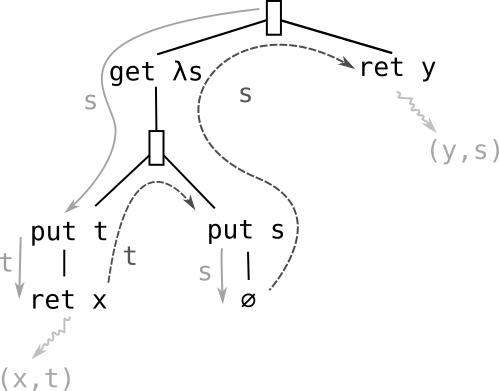
\includegraphics[scale=0.7]{sections/putR}
  \caption{Illustration of state-restoring put}
  \label{fig:putR}
\end{figure}

To help build understanding for \ensuremath{\Varid{put}_{\scaleobj{0.7}{\sf R}}}, Figure~\ref{fig:putR} shows the flow of
execution for the expression \ensuremath{(\Varid{put}_{\scaleobj{0.7}{\sf R}}\;\Varid{t}\mathbin{\hstretch{0.7}{>\!\!>}}\Varid{ret}\;\Varid{x})\mathbin{\talloblong}\Varid{ret}\;\Varid{y}}. Initially, the
state is \ensuremath{\Varid{s}}; it gets modified to \ensuremath{\Varid{t}} at the \ensuremath{\Varid{put}\;\Varid{t}} node after which the value
\ensuremath{\Varid{x}} is output with the working state \ensuremath{\Varid{t}}. Then, because we found a result, we
backtrack (since we're using global-state semantics, the state modification
caused by \ensuremath{\Varid{put}\;\Varid{t}} is not reversed), arriving in the \ensuremath{\Varid{side}} operation branch. The
\ensuremath{\Varid{put}\;\Varid{s}} operation is executed, which resets the state to \ensuremath{\Varid{s}}, and then the
branch immediately fails, so we backtrack to the right branch of the topmost
\ensuremath{(\talloblong)}. There the value \ensuremath{\Varid{y}} is output with working state \ensuremath{\Varid{s}}.

For some further intuition about \ensuremath{\Varid{put}_{\scaleobj{0.7}{\sf R}}}, consider \ensuremath{\Varid{put}_{\scaleobj{0.7}{\sf R}}\;\Varid{s}\mathbin{\hstretch{0.7}{>\!\!>}}\Varid{comp}} where \ensuremath{\Varid{comp}} is some arbitrary computation:
\begin{hscode}\SaveRestoreHook
\column{B}{@{}>{\hspre}l<{\hspost}@{}}%
\column{7}{@{}>{\hspre}l<{\hspost}@{}}%
\column{9}{@{}>{\hspre}l<{\hspost}@{}}%
\column{E}{@{}>{\hspre}l<{\hspost}@{}}%
\>[7]{}\Varid{put}_{\scaleobj{0.7}{\sf R}}\;\Varid{s}\mathbin{\hstretch{0.7}{>\!\!>}}\Varid{comp}{}\<[E]%
\\
\>[B]{}\mathbin{=}{}\<[7]%
\>[7]{}(\Varid{get}\mathrel{\hstretch{0.7}{>\!\!>\!\!=}}\lambda \Varid{s}_{0}\to \Varid{put}\;\Varid{s}\mathbin{\talloblong}\Varid{side}\;(\Varid{put}\;\Varid{s}_{0}))\mathbin{\hstretch{0.7}{>\!\!>}}\Varid{comp}{}\<[E]%
\\
\>[B]{}\mathbin{=}{}\<[9]%
\>[9]{}\mbox{\commentbegin  monad law, left-distributivity \eqref{eq:bind-mplus-dist}  \commentend}{}\<[E]%
\\
\>[B]{}\hsindent{7}{}\<[7]%
\>[7]{}\Varid{get}\mathrel{\hstretch{0.7}{>\!\!>\!\!=}}\lambda \Varid{s}_{0}\to (\Varid{put}\;\Varid{s}\mathbin{\hstretch{0.7}{>\!\!>}}\Varid{comp})\mathbin{\talloblong}(\Varid{side}\;(\Varid{put}\;\Varid{s}_{0})\mathbin{\hstretch{0.7}{>\!\!>}}\Varid{comp}){}\<[E]%
\\
\>[B]{}\mathbin{=}{}\<[9]%
\>[9]{}\mbox{\commentbegin  by \eqref{eq:bind-mzero-zero} \ensuremath{\Varid{\varnothing}\mathbin{\hstretch{0.7}{>\!\!>}}\Varid{comp}\mathrel{=}\Varid{\varnothing}}, monad laws  \commentend}{}\<[E]%
\\
\>[B]{}\hsindent{7}{}\<[7]%
\>[7]{}\Varid{get}\mathrel{\hstretch{0.7}{>\!\!>\!\!=}}\lambda \Varid{s}_{0}\to (\Varid{put}\;\Varid{s}\mathbin{\hstretch{0.7}{>\!\!>}}\Varid{comp})\mathbin{\talloblong}\Varid{side}\;(\Varid{put}\;\Varid{s}_{0})~~.{}\<[E]%
\ColumnHook
\end{hscode}\resethooks
Thanks to left-distributivity \eqref{eq:bind-mplus-dist}, \ensuremath{(\mathbin{\hstretch{0.7}{>\!\!>}}\Varid{comp})} is promoted into \ensuremath{(\talloblong)}.
Furthermore, the \ensuremath{(\mathbin{\hstretch{0.7}{>\!\!>}}\Varid{comp})} after \ensuremath{\Varid{side}\;(\Varid{put}\;\Varid{s}_{0})} is discarded by
\eqref{eq:bind-mzero-zero}.
In words, \ensuremath{\Varid{put}_{\scaleobj{0.7}{\sf R}}\;\Varid{s}\mathbin{\hstretch{0.7}{>\!\!>}}\Varid{comp}} saves the current state, computes \ensuremath{\Varid{comp}} using state \ensuremath{\Varid{s}}, and restores the saved state!
The subscript \ensuremath{\Conid{R}} stands for ``restore.''
Note also that \ensuremath{(\Varid{put}_{\scaleobj{0.7}{\sf R}}\;\Varid{s}\mathbin{\hstretch{0.7}{>\!\!>}}\Varid{m}_{1})\mathbin{\hstretch{0.7}{>\!\!>}}\Varid{m}_{2}\mathrel{=}\Varid{put}_{\scaleobj{0.7}{\sf R}}\;\Varid{s}\mathbin{\hstretch{0.7}{>\!\!>}}(\Varid{m}_{1}\mathbin{\hstretch{0.7}{>\!\!>}}\Varid{m}_{2})} --- the state restoration happens in the end.

The behaviour of \ensuremath{\Varid{put}_{\scaleobj{0.7}{\sf R}}} is rather tricky. It is instructive comparing
\begin{enumerate}[label=(\alph*)]
\item \ensuremath{\Varid{return}\;\Varid{x}},  \label{ex:putR-pitfalls-1}
\item \ensuremath{\Varid{put}\;\Varid{s}\mathbin{\hstretch{0.7}{>\!\!>}}\Varid{return}\;\Varid{x}}, \label{ex:putR-pitfalls-2}
\item \ensuremath{\Varid{put}_{\scaleobj{0.7}{\sf R}}\;\Varid{s}\mathbin{\hstretch{0.7}{>\!\!>}}\Varid{return}\;\Varid{x}}. \label{ex:putR-pitfalls-3}
\end{enumerate}
When run in initial state \ensuremath{\Varid{s}_{0}}, they all yield \ensuremath{\Varid{x}} as the result.
The final states after running \ref{ex:putR-pitfalls-1}, \ref{ex:putR-pitfalls-2} and \ref{ex:putR-pitfalls-3} are \ensuremath{\Varid{s}_{0}}, \ensuremath{\Varid{s}} and \ensuremath{\Varid{s}_{0}}, respectively.
However, \ref{ex:putR-pitfalls-3} does {\em not} behave identically to \ref{ex:putR-pitfalls-1} in all contexts!
For example, in the context \ensuremath{(\mathbin{\hstretch{0.7}{>\!\!>}}\Varid{get})}, we can tell them apart:
\ensuremath{\Varid{return}\;\Varid{x}\mathbin{\hstretch{0.7}{>\!\!>}}\Varid{get}} returns \ensuremath{\Varid{s}_{0}}, while \ensuremath{\Varid{put}_{\scaleobj{0.7}{\sf R}}\;\Varid{s}\mathbin{\hstretch{0.7}{>\!\!>}}\Varid{return}\;\Varid{x}\mathbin{\hstretch{0.7}{>\!\!>}}\Varid{get}} returns \ensuremath{\Varid{s}}, even though the program yields final state \ensuremath{\Varid{s}_{0}}.

We wish that \ensuremath{\Varid{put}_{\scaleobj{0.7}{\sf R}}}, when run with a global state, satisfies laws \eqref{eq:put-put} through \eqref{eq:mplus-bind-dist} ---
the state laws and the \emph{local} state laws.
If so, one could take a program written for a local state monad, replace all occurrences of \ensuremath{\Varid{put}} by \ensuremath{\Varid{put}_{\scaleobj{0.7}{\sf R}}}, and run the program with a global state.
Unfortunately this is not the case: \ensuremath{\Varid{put}_{\scaleobj{0.7}{\sf R}}} does satisfy {\bf put-put}~\eqref{eq:put-put} and {\bf put-get}~\eqref{eq:put-get}, but {\bf get-put}~\eqref{eq:get-put} fails ---
\ensuremath{\Varid{get}\mathrel{\hstretch{0.7}{>\!\!>\!\!=}}\Varid{put}_{\scaleobj{0.7}{\sf R}}} and \ensuremath{\Varid{return}\;()} can be
differentiated by some contexts, for example \ensuremath{(\mathbin{\hstretch{0.7}{>\!\!>}}\Varid{put}\;\Varid{t})}.
To see that, we calculate:
\begin{hscode}\SaveRestoreHook
\column{B}{@{}>{\hspre}l<{\hspost}@{}}%
\column{7}{@{}>{\hspre}l<{\hspost}@{}}%
\column{9}{@{}>{\hspre}l<{\hspost}@{}}%
\column{E}{@{}>{\hspre}l<{\hspost}@{}}%
\>[7]{}(\Varid{get}\mathrel{\hstretch{0.7}{>\!\!>\!\!=}}\Varid{put}_{\scaleobj{0.7}{\sf R}})\mathbin{\hstretch{0.7}{>\!\!>}}\Varid{put}\;\Varid{t}{}\<[E]%
\\
\>[B]{}\mathbin{=}{}\<[7]%
\>[7]{}(\Varid{get}\mathrel{\hstretch{0.7}{>\!\!>\!\!=}}\lambda \Varid{s}\to \Varid{get}\mathrel{\hstretch{0.7}{>\!\!>\!\!=}}\lambda \Varid{s}_{0}\to \Varid{put}\;\Varid{s}\mathbin{\talloblong}\Varid{side}\;(\Varid{put}\;\Varid{s}_{0}))\mathbin{\hstretch{0.7}{>\!\!>}}\Varid{put}\;\Varid{t}{}\<[E]%
\\
\>[B]{}\mathbin{=}{}\<[9]%
\>[9]{}\mbox{\commentbegin  {\bf get-get}  \commentend}{}\<[E]%
\\
\>[B]{}\hsindent{7}{}\<[7]%
\>[7]{}(\Varid{get}\mathrel{\hstretch{0.7}{>\!\!>\!\!=}}\lambda \Varid{s}\to \Varid{put}\;\Varid{s}\mathbin{\talloblong}\Varid{side}\;(\Varid{put}\;\Varid{s}))\mathbin{\hstretch{0.7}{>\!\!>}}\Varid{put}\;\Varid{t}{}\<[E]%
\\
\>[B]{}\mathbin{=}{}\<[9]%
\>[9]{}\mbox{\commentbegin  monad laws, left-distributivity  \commentend}{}\<[E]%
\\
\>[B]{}\hsindent{7}{}\<[7]%
\>[7]{}\Varid{get}\mathrel{\hstretch{0.7}{>\!\!>\!\!=}}\lambda \Varid{s}\to (\Varid{put}\;\Varid{s}\mathbin{\hstretch{0.7}{>\!\!>}}\Varid{put}\;\Varid{t})\mathbin{\talloblong}\Varid{side}\;(\Varid{put}\;\Varid{s}){}\<[E]%
\\
\>[B]{}\mathbin{=}{}\<[9]%
\>[9]{}\mbox{\commentbegin  {\bf put-put}  \commentend}{}\<[E]%
\\
\>[B]{}\hsindent{7}{}\<[7]%
\>[7]{}\Varid{get}\mathrel{\hstretch{0.7}{>\!\!>\!\!=}}\lambda \Varid{s}\to \Varid{put}\;\Varid{t}\mathbin{\talloblong}\Varid{side}\;(\Varid{put}\;\Varid{s})~~.{}\<[E]%
\ColumnHook
\end{hscode}\resethooks
Meanwhile, \ensuremath{\Varid{return}\;()\mathbin{\hstretch{0.7}{>\!\!>}}\Varid{put}\;\Varid{t}\mathrel{=}\Varid{put}\;\Varid{t}}, which does not behave in the same way as \ensuremath{\Varid{get}\mathrel{\hstretch{0.7}{>\!\!>\!\!=}}\lambda \Varid{s}\to \Varid{put}\;\Varid{t}\mathbin{\talloblong}\Varid{side}\;(\Varid{put}\;\Varid{s})} when $s \neq t$.

In a global-state setting, the left-distributivity law
\eqref{eq:bind-mplus-dist} makes it tricky to reason about combinations of
\ensuremath{(\talloblong)} and \ensuremath{(\mathrel{\hstretch{0.7}{>\!\!>\!\!=}})} operators. Suppose we have a program \ensuremath{(\Varid{m}\mathbin{\talloblong}\Varid{n})}, and we
construct an extended program by binding a continuation \ensuremath{\Varid{f}} to it such that we
get \ensuremath{(\Varid{m}\mathbin{\talloblong}\Varid{n})\mathrel{\hstretch{0.7}{>\!\!>\!\!=}}\Varid{f}} (where \ensuremath{\Varid{f}} might modify the state). Under global-state
semantics, the evaluation of the right branch is influenced by the state
modifications performed by evaluating the left branch. So by
\eqref{eq:bind-mplus-dist}, this means that when we get to evaluating the \ensuremath{\Varid{n}}
subprogram in the extended program, it will do so with a different initial state
(the one obtained after running \ensuremath{\Varid{m}\mathrel{\hstretch{0.7}{>\!\!>\!\!=}}\Varid{f}}) compared to the initial state in the
original program (the one obtained by running \ensuremath{\Varid{m}}). In other words, placing our
program in a different context changed the meaning of one of its subprograms. So
it is difficult to reason about programs compositionally in this
setting---some properties hold only when we take the entire program into
consideration.

It turns out that all properties we need do hold, provided that {\em all}
occurrences of \ensuremath{\Varid{put}} are replaced by \ensuremath{\Varid{put}_{\scaleobj{0.7}{\sf R}}}---problematic contexts such as
\ensuremath{\Varid{put}\;\Varid{t}} above are thus ruled out. However, that ``all \ensuremath{\Varid{put}} are replaced by
\ensuremath{\Varid{put}_{\scaleobj{0.7}{\sf R}}}'' is a global property, and to properly talk about it we have to formally
define contexts, which is what we will do in Section~\ref{sec:ctxt-trans}.
Notice though, that simulation of local state semantics by judicious use of
\ensuremath{\Varid{put}_{\scaleobj{0.7}{\sf R}}} does not avoid the unnecessary copying mentioned in
Section~\ref{sec:space-usage}, it merely makes it explicit in the program.
We will address this shortcoming in Section~\ref{sec:backtrack-gs}.
\section{Proving the $\mathit{put}_{\text{R}}$ Transformation Correct For a Given Implementation}
Before we tackle the general proof of correctness of the \ensuremath{\Varid{put}_{\scaleobj{0.7}{\sf R}}} transformation
correct, we dip our toes into something a bit more straightforward: showing that
the transformation is correct for specific implementations of global and local
state. This lets us use a somewhat more concrete setting to introduce some
infrastructure needed for the more general proof, as well as demonstrate a case
study of a fold fusion proof (TODO: citation), an elegant and powerful technique
that is interesting in its own right.

In the previous sections we have been mixing syntax and semantics,
which we avoid in this section by defining the program syntax as a free monad
(TODO: citation).
This way we avoid the need for a type-level distinction between programs
with local-state semantics and programs with global-state semantics.
\begin{hscode}\SaveRestoreHook
\column{B}{@{}>{\hspre}l<{\hspost}@{}}%
\column{3}{@{}>{\hspre}l<{\hspost}@{}}%
\column{7}{@{}>{\hspre}l<{\hspost}@{}}%
\column{11}{@{}>{\hspre}l<{\hspost}@{}}%
\column{15}{@{}>{\hspre}l<{\hspost}@{}}%
\column{24}{@{}>{\hspre}l<{\hspost}@{}}%
\column{E}{@{}>{\hspre}l<{\hspost}@{}}%
\>[B]{}\mathbf{data}\;\Conid{Free}\;\Varid{f}\;\Varid{a}\;\mathbf{where}{}\<[E]%
\\
\>[B]{}\hsindent{3}{}\<[3]%
\>[3]{}\Conid{Ret}\mathbin{::}\Varid{a}{}\<[24]%
\>[24]{}\to \Conid{Free}\;\Varid{f}\;\Varid{a}{}\<[E]%
\\
\>[B]{}\hsindent{3}{}\<[3]%
\>[3]{}\Conid{Op}{}\<[7]%
\>[7]{}\mathbin{::}\Varid{f}\;(\Conid{Free}\;\Varid{f}\;\Varid{a}){}\<[24]%
\>[24]{}\to \Conid{Free}\;\Varid{f}\;\Varid{a}{}\<[E]%
\\[\blanklineskip]%
\>[B]{}\mathbf{instance}\;\Conid{Functor}\;\Varid{f}\Rightarrow \Conid{Functor}\;(\Conid{Free}\;\Varid{f})\;\mathbf{where}{}\<[E]%
\\
\>[B]{}\hsindent{3}{}\<[3]%
\>[3]{}\Varid{fmap}\;\Varid{f}\;(\Conid{Ret}\;\Varid{x})\mathrel{=}\Conid{Ret}\;(\Varid{f}\;\Varid{x}){}\<[E]%
\\
\>[B]{}\hsindent{3}{}\<[3]%
\>[3]{}\Varid{fmap}\;\Varid{f}\;(\Conid{Op}\;{}\<[15]%
\>[15]{}\Varid{o})\mathrel{=}\Conid{Op}\;(\Varid{fmap}\;(\Varid{fmap}\;\Varid{f})\;\Varid{o}){}\<[E]%
\\[\blanklineskip]%
\>[B]{}\mathbf{instance}\;\Conid{Functor}\;\Varid{f}\Rightarrow \Conid{Monad}\;(\Conid{Free}\;\Varid{f})\;\mathbf{where}{}\<[E]%
\\
\>[B]{}\hsindent{3}{}\<[3]%
\>[3]{}\Varid{return}{}\<[11]%
\>[11]{}\mathrel{=}\Varid{pure}{}\<[E]%
\\
\>[B]{}\hsindent{3}{}\<[3]%
\>[3]{}\Conid{Ret}\;\Varid{x}\mathrel{\hstretch{0.7}{>\!\!>\!\!=}}\Varid{g}\mathrel{=}\Varid{g}\;\Varid{x}{}\<[E]%
\\
\>[B]{}\hsindent{3}{}\<[3]%
\>[3]{}\Conid{Op}\;\Varid{op}\mathrel{\hstretch{0.7}{>\!\!>\!\!=}}\Varid{g}\mathrel{=}\Conid{Op}\;(\Varid{fmap}\;(\mathrel{\hstretch{0.7}{>\!\!>\!\!=}}\Varid{g})\;\Varid{op}){}\<[E]%
\ColumnHook
\end{hscode}\resethooks
The state and nondeterminism interfaces are provided as ``algebras''. These are
functors equipped with a constructor for each operation they support.
\begin{hscode}\SaveRestoreHook
\column{B}{@{}>{\hspre}l<{\hspost}@{}}%
\column{3}{@{}>{\hspre}l<{\hspost}@{}}%
\column{5}{@{}>{\hspre}l<{\hspost}@{}}%
\column{12}{@{}>{\hspre}l<{\hspost}@{}}%
\column{25}{@{}>{\hspre}l<{\hspost}@{}}%
\column{E}{@{}>{\hspre}l<{\hspost}@{}}%
\>[3]{}\mathbf{data}\;\Conid{StateF}\;\Varid{a}\;\mathbf{where}{}\<[E]%
\\
\>[3]{}\hsindent{2}{}\<[5]%
\>[5]{}\Conid{Get}{}\<[12]%
\>[12]{}\mathbin{::}(\Conid{S}\to \Varid{a}){}\<[25]%
\>[25]{}\to \Conid{StateF}\;\Varid{a}{}\<[E]%
\\
\>[3]{}\hsindent{2}{}\<[5]%
\>[5]{}\Conid{Put}{}\<[12]%
\>[12]{}\mathbin{::}\Conid{S}\to \Varid{a}{}\<[25]%
\>[25]{}\to \Conid{StateF}\;\Varid{a}{}\<[E]%
\\
\>[3]{}\hsindent{2}{}\<[5]%
\>[5]{}\mathbf{deriving}\;\Conid{Functor}{}\<[E]%
\\[\blanklineskip]%
\>[3]{}\mathbf{data}\;\Conid{NondetF}\;\Varid{a}\;\mathbf{where}{}\<[E]%
\\
\>[3]{}\hsindent{2}{}\<[5]%
\>[5]{}\Varid{\varnothing}{}\<[12]%
\>[12]{}\mathbin{::}\Conid{NondetF}\;\Varid{a}{}\<[E]%
\\
\>[3]{}\hsindent{2}{}\<[5]%
\>[5]{}(\talloblong){}\<[12]%
\>[12]{}\mathbin{::}\Varid{a}\to \Varid{a}\to \Conid{NondetF}\;\Varid{a}{}\<[E]%
\\
\>[3]{}\hsindent{2}{}\<[5]%
\>[5]{}\mathbf{deriving}\;\Conid{Functor}{}\<[E]%
\ColumnHook
\end{hscode}\resethooks
In this encoding, the type \ensuremath{\Conid{Free}\;\Conid{StateF}\;\Varid{a}} represents stateful computations, and
similarly the type \ensuremath{\Conid{Free}\;\Conid{NondetF}\;\Varid{a}} represents nondeterministic computations.
Note that in this representation, our programs are written in a
continuation-passing style. For instance, where in the previous section we would
have written \ensuremath{\Varid{put}\;\Varid{t}\mathbin{\hstretch{0.7}{>\!\!>}}\Varid{get}}, we now write \ensuremath{\Conid{Op}\;(\Conid{Put}\;\Varid{t}\;(\Conid{Op}\;\Conid{Get}))}.
Computations with multiple effects can be typed with a sum type \ensuremath{(\mathbin{+})} over types
of kind \ensuremath{\mathbin{*}\to \mathbin{*}}.
\begin{hscode}\SaveRestoreHook
\column{B}{@{}>{\hspre}l<{\hspost}@{}}%
\column{3}{@{}>{\hspre}l<{\hspost}@{}}%
\column{5}{@{}>{\hspre}l<{\hspost}@{}}%
\column{E}{@{}>{\hspre}l<{\hspost}@{}}%
\>[3]{}\mathbf{data}\;(\Varid{f}\mathbin{+}\Varid{g})\;\Varid{a}\;\mathbf{where}{}\<[E]%
\\
\>[3]{}\hsindent{2}{}\<[5]%
\>[5]{}\Conid{Inl}\mathbin{::}\Varid{f}\;\Varid{a}\to (\Varid{f}\mathbin{+}\Varid{g})\;\Varid{a}{}\<[E]%
\\
\>[3]{}\hsindent{2}{}\<[5]%
\>[5]{}\Conid{Inr}\mathbin{::}\Varid{g}\;\Varid{a}\to (\Varid{f}\mathbin{+}\Varid{g})\;\Varid{a}{}\<[E]%
\\
\>[3]{}\hsindent{2}{}\<[5]%
\>[5]{}\mathbf{deriving}\;\Conid{Functor}{}\<[E]%
\ColumnHook
\end{hscode}\resethooks
The type \ensuremath{\Conid{Free}\;(\Conid{NondetF}\mathbin{+}\Conid{StateF})\;\Varid{a}} is one way to encode programs which have
both nondeterminism and state as effects. So is \ensuremath{\Conid{Free}\;(\Conid{StateF}\mathbin{+}\Conid{NondetF})\;\Varid{a}}, or
more generally \ensuremath{\Conid{Functor}\;\Varid{f}\Rightarrow \Conid{Free}\;(\Conid{StateF}\mathbin{+}(\Conid{NondetF}\mathbin{+}\Varid{f}))\;\Varid{a}} (where \ensuremath{\Varid{f}} may
introduce additional effects). 
Where in the previous section we would have written \ensuremath{\Varid{put}\;\Varid{t}\mathbin{\hstretch{0.7}{>\!\!>}}\Varid{\varnothing}}, we now
write \ensuremath{\Conid{Op}\;(\Conid{Inr}\;(\Conid{Put}\;\Varid{t}\;(\Conid{Op}\;(\Conid{Inl}\;\Varid{\varnothing}))))\mathbin{::}\Conid{Free}\;(\Conid{NondetF}\mathbin{+}\Conid{StateF})\;\Varid{a}}. We will
later introduce notation to make our syntax a bit less noisy.
The \ensuremath{(\mathbin{+})} type is morally commutative, associative, and has a zero element:
\begin{hscode}\SaveRestoreHook
\column{B}{@{}>{\hspre}l<{\hspost}@{}}%
\column{9}{@{}>{\hspre}l<{\hspost}@{}}%
\column{E}{@{}>{\hspre}l<{\hspost}@{}}%
\>[B]{}\Varid{comm}{}\<[9]%
\>[9]{}\mathbin{::}(\Conid{Functor}\;\Varid{f},\Conid{Functor}\;\Varid{g})\Rightarrow \Conid{Free}\;(\Varid{f}\mathbin{+}\Varid{g})\;\Varid{a}\to \Conid{Free}\;(\Varid{g}\mathbin{+}\Varid{f})\;\Varid{a}{}\<[E]%
\\
\>[B]{}\Varid{assocl}{}\<[9]%
\>[9]{}\mathbin{::}(\Conid{Functor}\;\Varid{f},\Conid{Functor}\;\Varid{g},\Conid{Functor}\;\Varid{h}){}\<[E]%
\\
\>[9]{}\Rightarrow \Conid{Free}\;(\Varid{f}\mathbin{+}(\Varid{g}\mathbin{+}\Varid{h}))\;\Varid{a}\to \Conid{Free}\;((\Varid{f}\mathbin{+}\Varid{g})\mathbin{+}\Varid{h})\;\Varid{a}{}\<[E]%
\\
\>[B]{}\Varid{assocr}{}\<[9]%
\>[9]{}\mathbin{::}(\Conid{Functor}\;\Varid{f},\Conid{Functor}\;\Varid{g},\Conid{Functor}\;\Varid{h}){}\<[E]%
\\
\>[9]{}\Rightarrow \Conid{Free}\;((\Varid{f}\mathbin{+}\Varid{g})\mathbin{+}\Varid{h})\;\Varid{a}\to \Conid{Free}\;(\Varid{f}\mathbin{+}(\Varid{g}\mathbin{+}\Varid{h}))\;\Varid{a}{}\<[E]%
\\[\blanklineskip]%
\>[B]{}\mathbf{data}\;\Conid{Nil}\;\Varid{a}\;\mathbf{deriving}\;\Conid{Functor}{}\<[E]%
\\[\blanklineskip]%
\>[B]{}\Varid{hNil}{}\<[9]%
\>[9]{}\mathbin{::}\Conid{Free}\;\Conid{Nil}\;\Varid{a}\to \Varid{a}{}\<[E]%
\\
\>[B]{}\Varid{hNil}\;(\Conid{Ret}\;\Varid{x})\mathrel{=}\Varid{x}{}\<[E]%
\\
\>[B]{}\mbox{\onelinecomment  other cases cannot occur}{}\<[E]%
\ColumnHook
\end{hscode}\resethooks
This zero element is an empty ``effect set'': a program of type \ensuremath{\Conid{Free}\;\Conid{Nil}\;\Varid{a}}
represents a program that computes an \ensuremath{\Varid{a}} without relying on any effects (this
type is commutative with just the type \ensuremath{\Varid{a}}).

With the \ensuremath{\Conid{Free}}-based encoding we can not only write programs
with effect sets composed from smaller effect sets, we can also write the {\em
handlers} for these effect sets compositionally.
For state and nondeterminism, we respectively write the following types for
their ``compositional'' handlers:
\begin{hscode}\SaveRestoreHook
\column{B}{@{}>{\hspre}l<{\hspost}@{}}%
\column{10}{@{}>{\hspre}l<{\hspost}@{}}%
\column{41}{@{}>{\hspre}l<{\hspost}@{}}%
\column{E}{@{}>{\hspre}l<{\hspost}@{}}%
\>[B]{}\Varid{hState}{}\<[10]%
\>[10]{}\mathbin{::}\Conid{Functor}\;\Varid{f}\Rightarrow \Conid{Free}\;(\Conid{StateF}{}\<[41]%
\>[41]{}\mathbin{+}\Varid{f})\;\Varid{a}\to (\Conid{S}\to \Conid{Free}\;\Varid{f}\;(\Varid{a},\Conid{S})){}\<[E]%
\\
\>[B]{}\Varid{hNondet}{}\<[10]%
\>[10]{}\mathbin{::}\Conid{Functor}\;\Varid{f}\Rightarrow \Conid{Free}\;(\Conid{NondetF}{}\<[41]%
\>[41]{}\mathbin{+}\Varid{f})\;\Varid{a}\to \Conid{Free}\;\Varid{f}\;(\Conid{Bag}\;\Varid{a}){}\<[E]%
\ColumnHook
\end{hscode}\resethooks
Here the \ensuremath{\Conid{Bag}} type represents a multiset data structure. We give a simple
example implementation:
\begin{hscode}\SaveRestoreHook
\column{B}{@{}>{\hspre}l<{\hspost}@{}}%
\column{3}{@{}>{\hspre}l<{\hspost}@{}}%
\column{31}{@{}>{\hspre}l<{\hspost}@{}}%
\column{53}{@{}>{\hspre}l<{\hspost}@{}}%
\column{E}{@{}>{\hspre}l<{\hspost}@{}}%
\>[3]{}\mathbf{newtype}\;\Conid{Bag}\;\Varid{a}\mathrel{=}\Conid{Bag}\;[\mskip1.5mu \Varid{a}\mskip1.5mu]\;\mathbf{deriving}\;\Conid{Functor}{}\<[E]%
\\[\blanklineskip]%
\>[3]{}\mathbf{instance}\;\Conid{Semigroup}\;(\Conid{Bag}\;\Varid{a})\;{}\<[31]%
\>[31]{}\mathbf{where}\;\Conid{Bag}\;\Varid{l}\mathbin{\Diamond}\Conid{Bag}\;\Varid{r}{}\<[53]%
\>[53]{}\mathrel{=}\Conid{Bag}\;(\Varid{l}\mathbin{+\!\!\!\!\!+}\Varid{r}){}\<[E]%
\\[\blanklineskip]%
\>[3]{}\mathbf{instance}\;\Conid{Monoid}\;(\Conid{Bag}\;\Varid{a})\;{}\<[31]%
\>[31]{}\mathbf{where}\;\Varid{mempty}{}\<[53]%
\>[53]{}\mathrel{=}\Conid{Bag}\;[\mskip1.5mu \mskip1.5mu]{}\<[E]%
\\[\blanklineskip]%
\>[3]{}\mathbf{instance}\;\Conid{Eq}\;(\Conid{Bag}\;\Varid{a})\;{}\<[31]%
\>[31]{}\mathbf{where}\;\Conid{Bag}\;\Varid{l}\doubleequals\Conid{Bag}\;\Varid{r}{}\<[53]%
\>[53]{}\mathrel{=}\Varid{sort}\;\Varid{l}\doubleequals\Varid{sort}\;\Varid{r}{}\<[E]%
\\[\blanklineskip]%
\>[3]{}\Varid{singleton}\mathbin{::}\Varid{a}\to \Conid{Bag}\;\Varid{a}{}\<[E]%
\\
\>[3]{}\Varid{singleton}\;\Varid{x}\mathrel{=}\Conid{Bag}\;[\mskip1.5mu \Varid{x}\mskip1.5mu]{}\<[E]%
\\[\blanklineskip]%
\>[3]{}\Varid{elem}\mathbin{::}\Conid{Eq}\;\Varid{a}\Rightarrow \Varid{a}\to \Conid{Bag}\;\Varid{a}\to \Conid{Int}{}\<[E]%
\\
\>[3]{}\Varid{elem}\;\Varid{x}\;(\Conid{Bag}\;\Varid{xs})\mathrel{=}\Varid{length}\;(\Varid{filter}\;(\doubleequals\Varid{x})\;\Varid{xs}){}\<[E]%
\\[\blanklineskip]%
\>[3]{}\Varid{bagFlatten}\mathbin{::}\Conid{Bag}\;(\Conid{Bag}\;\Varid{a})\to \Conid{Bag}\;\Varid{a}{}\<[E]%
\\
\>[3]{}\Varid{bagFlatten}\;(\Conid{Bag}\;\Varid{bags})\mathrel{=}\Conid{Bag}\;(\Varid{concat}\;\Varid{bags}){}\<[E]%
\ColumnHook
\end{hscode}\resethooks
The type of the \ensuremath{\Varid{hState}} and \ensuremath{\Varid{hNondet}} handlers indicate that they handle one
effect of the effect set of the program, yielding a new effectful program where
the effect set contains all the remaining effects.  This is a bit reminiscent
of a ``linked list'' of effects. Like a linked list, a ``nil'' element is
needed to terminate the list; this is provided to us by the \ensuremath{\Conid{Nil}} type.

For instance, we can compose a handler \ensuremath{\Varid{hLocal}} for local state semantics out of
the ``atomic'' handlers for state and nondeterminism.
We will only be interested in the results of the computation, not the final
states, so the final step of our local state handler is to throw away the state
information (with \ensuremath{\Varid{fmap}\;\Varid{fst}}).
\begin{hscode}\SaveRestoreHook
\column{B}{@{}>{\hspre}l<{\hspost}@{}}%
\column{10}{@{}>{\hspre}l<{\hspost}@{}}%
\column{E}{@{}>{\hspre}l<{\hspost}@{}}%
\>[B]{}\Varid{hLocal'}{}\<[10]%
\>[10]{}\mathbin{::}\Conid{Free}\;(\Conid{StateF}\mathbin{+}(\Conid{NondetF}\mathbin{+}\Conid{Nil}))\;\Varid{a}\to (\Conid{S}\to \Conid{Bag}\;(\Varid{a},\Conid{S})){}\<[E]%
\\
\>[B]{}\Varid{hLocal'}{}\<[10]%
\>[10]{}\mathrel{=}\Varid{fmap}\;(\Varid{hNil}\mathbin{\cdot}\Varid{hNondet})\mathbin{\cdot}\Varid{hState}{}\<[E]%
\\[\blanklineskip]%
\>[B]{}\Varid{hLocal}{}\<[10]%
\>[10]{}\mathbin{::}\Conid{Free}\;(\Conid{StateF}\mathbin{+}(\Conid{NondetF}\mathbin{+}\Conid{Nil}))\;\Varid{a}\to (\Conid{S}\to \Conid{Bag}\;\Varid{a}){}\<[E]%
\\
\>[B]{}\Varid{hLocal}{}\<[10]%
\>[10]{}\mathrel{=}\Varid{fmap}\;(\Varid{fmap}\;\Varid{fst})\mathbin{\cdot}\Varid{hLocal'}{}\<[E]%
\ColumnHook
\end{hscode}\resethooks
In other words, local state semantics is the semantics where we
nondeterministically choose between different stateful computations. This
matches our intuition of local state semantics: if we can picture stateful,
nondeterministic programs as trees, then local state semantics is the
interpretation of the tree where each result of the (nondeterministic, stateful)
computation corresponds to a path from root to leaf in the tree. One can compute
each of these paths entirely independently from the other paths. 
Later on, we shall prove that this composition forms a valid
implementation of local state semantics.

Global state semantics can be implemented by simply inverting the order of the
handlers: rather than nondeterministically choosing between stateful
computations as local state does, in global state semantics we'll run a
single state through a nondeterministic computation.
Just like with the local state handler, we are not interested in the final state
of the computation, only in the results, so the final step of our handler is a
\ensuremath{\Varid{fmap}\;\Varid{fst}}.
\begin{hscode}\SaveRestoreHook
\column{B}{@{}>{\hspre}l<{\hspost}@{}}%
\column{11}{@{}>{\hspre}l<{\hspost}@{}}%
\column{E}{@{}>{\hspre}l<{\hspost}@{}}%
\>[B]{}\Varid{hGlobal'}{}\<[11]%
\>[11]{}\mathbin{::}\Conid{Free}\;(\Conid{NondetF}\mathbin{+}(\Conid{StateF}\mathbin{+}\Conid{Nil}))\;\Varid{a}\to (\Conid{S}\to (\Conid{Bag}\;\Varid{a},\Conid{S})){}\<[E]%
\\
\>[B]{}\Varid{hGlobal'}{}\<[11]%
\>[11]{}\mathrel{=}\Varid{fmap}\;\Varid{hNil}\mathbin{\cdot}\Varid{hState}\mathbin{\cdot}\Varid{hNondet}{}\<[E]%
\\[\blanklineskip]%
\>[B]{}\Varid{hGlobal}{}\<[11]%
\>[11]{}\mathbin{::}\Conid{Free}\;(\Conid{NondetF}\mathbin{+}(\Conid{StateF}\mathbin{+}\Conid{Nil}))\;\Varid{a}\to (\Conid{S}\to \Conid{Bag}\;\Varid{a}){}\<[E]%
\\
\>[B]{}\Varid{hGlobal}{}\<[11]%
\>[11]{}\mathrel{=}\Varid{fmap}\;\Varid{fst}\mathbin{\cdot}\Varid{hGlobal'}{}\<[E]%
\ColumnHook
\end{hscode}\resethooks
We argue the correctness of \ensuremath{\Varid{hLocal}} and \ensuremath{\Varid{hGlobal}} (with respect to laws of
respectively local and global state semantics) in~\ref{sec:correctness-handlers}.

%From this point onwards, we will omit some technical details where confusion is
%unlikely to arise. In particular, we will omit the |Op|, |Inl| and |Inr|
%constructors from our programs. For example, when we should write
%|Op (Inl (Get (\x -> Op (Inr (p x `mplus` q x)))))| (an instance of the type
%|Free (StateF + NondetF) a|), we shall instead write
%|Get (\x -> p x `mplus` q x)|, and by this actually mean an element of the type
%|Free (StateF + NondetF) a| instead of the type |StateF (NondetF a)|.
%Moreover, in our notation the same term is also an instance of
%|Free (NondetF + StateF) a|, and of |Free| 

\subsection{Folds and Fold Fusion}
\label{sec:fold-fusion}
(TODO citations)
Rather than defining our handlers directly by writing a general recursive
function, we will write them as folds, a type of structural recursion.
\begin{hscode}\SaveRestoreHook
\column{B}{@{}>{\hspre}l<{\hspost}@{}}%
\column{3}{@{}>{\hspre}l<{\hspost}@{}}%
\column{25}{@{}>{\hspre}l<{\hspost}@{}}%
\column{E}{@{}>{\hspre}l<{\hspost}@{}}%
\>[3]{}\Varid{fold}\mathbin{::}\Conid{Functor}\;\Varid{f}\Rightarrow (\Varid{a}\to \Varid{r})\to (\Varid{f}\;\Varid{r}\to \Varid{r})\to \Conid{Free}\;\Varid{f}\;\Varid{r}\to \Varid{r}{}\<[E]%
\\
\>[3]{}\Varid{fold}\;\Varid{gen}\;\Varid{alg}\;(\Conid{Ret}\;\Varid{x}){}\<[25]%
\>[25]{}\mathrel{=}\Varid{gen}\;\Varid{x}{}\<[E]%
\\
\>[3]{}\Varid{fold}\;\Varid{gen}\;\Varid{alg}\;(\Conid{Op}\;\Varid{op}){}\<[25]%
\>[25]{}\mathrel{=}\Varid{alg}\;(\Varid{fmap}\;(\Varid{fold}\;\Varid{gen}\;\Varid{alg})\;\Varid{op}){}\<[E]%
\ColumnHook
\end{hscode}\resethooks
This more principled approach gives us more leverage when reasoning about our
programs, as certain laws hold for programs defined through fusion.
In particular, we are interested in the {\em fold fusion} law:
\begin{align*}
  \ensuremath{\Varid{h}\mathbin{\cdot}\Varid{fold}\;\Varid{gen}\;\Varid{alg}} & = \ensuremath{\Varid{fold}\;\Varid{gen'}\;\Varid{alg'}} \\
                     & \Uparrow \\
  \ensuremath{\Varid{h}\mathbin{\cdot}\Varid{gen}}          & = \ensuremath{\Varid{gen'}} \\
  \ensuremath{\Varid{h}\mathbin{\cdot}\Varid{alg}}          & = \ensuremath{\Varid{alg'}\mathbin{\cdot}\Varid{fmap}\;\Varid{h}}
\end{align*}
Informally, this law states that a post-processing step (\ensuremath{\Varid{h}}) following a fold
can, if certain conditions are met, be {\em fused} into the fold.
Moreover, it will soon become apparent that the fold fusion law is not only
helpful in proving two known programs equivalent, but in fact it can often help
in finding a fused program given a composition of two programs. This discovered
program will then be correct by construction.

We can define the state and nondeterminism handlers as folds.
\begin{hscode}\SaveRestoreHook
\column{B}{@{}>{\hspre}l<{\hspost}@{}}%
\column{3}{@{}>{\hspre}l<{\hspost}@{}}%
\column{5}{@{}>{\hspre}l<{\hspost}@{}}%
\column{32}{@{}>{\hspre}l<{\hspost}@{}}%
\column{37}{@{}>{\hspre}l<{\hspost}@{}}%
\column{E}{@{}>{\hspre}l<{\hspost}@{}}%
\>[B]{}\Varid{hState}\mathbin{::}\Conid{Functor}\;\Varid{f}\Rightarrow \Conid{Free}\;(\Conid{StateF}\mathbin{+}\Varid{f})\;\Varid{a}\to (\Conid{S}\to \Conid{Free}\;\Varid{f}\;(\Varid{a},\Conid{S})){}\<[E]%
\\
\>[B]{}\Varid{hState}\mathrel{=}\Varid{fold}\;\Varid{genState}\;\Varid{algState}{}\<[E]%
\\
\>[B]{}\hsindent{3}{}\<[3]%
\>[3]{}\mathbf{where}{}\<[E]%
\\
\>[3]{}\hsindent{2}{}\<[5]%
\>[5]{}\Varid{genState}\;\Varid{x}{}\<[32]%
\>[32]{}\mathrel{=}\lambda \Varid{s}\to \Conid{Ret}\;(\Varid{x},\Varid{s}){}\<[E]%
\\
\>[3]{}\hsindent{2}{}\<[5]%
\>[5]{}\Varid{algState}\;(\Conid{Inl}\;(\Conid{Get}\;\Varid{k})){}\<[32]%
\>[32]{}\mathrel{=}\lambda \Varid{s}\to \Varid{k}\;\Varid{s}\;\Varid{s}{}\<[E]%
\\
\>[3]{}\hsindent{2}{}\<[5]%
\>[5]{}\Varid{algState}\;(\Conid{Inl}\;(\Conid{Put}\;\Varid{t}\;\Varid{k})){}\<[32]%
\>[32]{}\mathrel{=}\lambda \anonymous \to \Varid{k}\;\Varid{t}{}\<[E]%
\\
\>[3]{}\hsindent{2}{}\<[5]%
\>[5]{}\Varid{algState}\;(\Conid{Inr}\;\Varid{p}){}\<[32]%
\>[32]{}\mathrel{=}\lambda \Varid{s}\to \Conid{Op}\;(\Varid{fmap}\;(\mathbin{\$}\Varid{s})\;\Varid{p}){}\<[E]%
\\[\blanklineskip]%
\>[B]{}\Varid{hNondet}\mathbin{::}\Conid{Functor}\;\Varid{f}\Rightarrow \Conid{Free}\;(\Conid{NondetF}\mathbin{+}\Varid{f})\;\Varid{a}\to \Conid{Free}\;\Varid{f}\;(\Conid{Bag}\;\Varid{a}){}\<[E]%
\\
\>[B]{}\Varid{hNondet}\mathrel{=}\Varid{fold}\;\Varid{genNondet}\;\Varid{algNondet}{}\<[E]%
\\
\>[B]{}\hsindent{3}{}\<[3]%
\>[3]{}\mathbf{where}{}\<[E]%
\\
\>[3]{}\hsindent{2}{}\<[5]%
\>[5]{}\Varid{genNondet}\;\Varid{x}{}\<[37]%
\>[37]{}\mathrel{=}\Conid{Ret}\;(\Varid{singleton}\;\Varid{x}){}\<[E]%
\\
\>[3]{}\hsindent{2}{}\<[5]%
\>[5]{}\Varid{algNondet}\;(\Conid{Inl}\;\Varid{\varnothing}){}\<[37]%
\>[37]{}\mathrel{=}\Conid{Ret}\;\Varid{mempty}{}\<[E]%
\\
\>[3]{}\hsindent{2}{}\<[5]%
\>[5]{}\Varid{algNondet}\;(\Conid{Inl}\;(\Varid{p}\mathbin{\talloblong}\Varid{q})){}\<[37]%
\>[37]{}\mathrel{=}(\mathbin{\Diamond})\mathrel{\raisebox{0.5\depth}{\scaleobj{0.5}{\langle}} \scaleobj{0.8}{\$} \raisebox{0.5\depth}{\scaleobj{0.5}{\rangle}}}\Varid{p}\mathrel{\raisebox{0.5\depth}{\scaleobj{0.5}{\langle}} \scaleobj{0.8}{\ast} \raisebox{0.5\depth}{\scaleobj{0.5}{\rangle}}}\Varid{q}{}\<[E]%
\\
\>[3]{}\hsindent{2}{}\<[5]%
\>[5]{}\Varid{algNondet}\;(\Conid{Inr}\;\Varid{op}){}\<[37]%
\>[37]{}\mathrel{=}\Conid{Op}\;\Varid{op}{}\<[E]%
\ColumnHook
\end{hscode}\resethooks
With our atomic handlers defined, we have also gained complete definitions for
\ensuremath{\Varid{hLocal}} and \ensuremath{\Varid{hGlobal}}, as we know how to compose them from the atomic
handlers. 

\subsubsection{A Note on Notation}
Before moving on, we will attempt to simplify our notation a bit, as it is
already becoming apparent that it's getting cumbersome, and this will
only get worse as we start reasoning with it.  For example, to write a ``get''
operator in a program typed with \ensuremath{\Conid{Free}\;(\Conid{NondetF}\mathbin{+}(\Conid{StateF}\mathbin{+}\Conid{NilF}))\;\Varid{a}} requires
us to write \ensuremath{\Conid{Inr}\;(\Conid{Inl}\;(\Conid{Op}\;(\Conid{Get}\;\Varid{k})))}. Even worse,
although we see the types 
\ensuremath{\Conid{Free}\;(\Conid{NondetF}\mathbin{+}(\Conid{StateF}\mathbin{+}\Conid{NilF}))\;\Varid{a}} and \ensuremath{\Conid{Free}\;(\Conid{StateF}\mathbin{+}(\Conid{NondetF}\mathbin{+}\Conid{NilF}))\;\Varid{a}} as
morally the same, to convert a value of one of them into the other requires some
tedious type gymnastics.
For instance, if we want \ensuremath{\Varid{hGlobal}} to operate on the same
type of programs as \ensuremath{\Varid{hLocal}}, we need to perform some intermediate transformations:
\begin{hscode}\SaveRestoreHook
\column{B}{@{}>{\hspre}l<{\hspost}@{}}%
\column{E}{@{}>{\hspre}l<{\hspost}@{}}%
\>[B]{}\Varid{hGlobal'}\mathbin{::}\Conid{Free}\;(\Conid{StateF}\mathbin{+}(\Conid{NondetF}\mathbin{+}\Conid{Nil}))\;\Varid{a}\to (\Conid{S}\to (\Conid{Bag}\;\Varid{a},\Conid{S})){}\<[E]%
\\
\>[B]{}\Varid{hGlobal'}\mathrel{=}\Varid{fmap}\;\Varid{hNil}\mathbin{\cdot}\Varid{hState}\mathbin{\cdot}\Varid{comm}\mathbin{\cdot}\Varid{hNondet}\mathbin{\cdot}\Varid{assocr}\mathbin{\cdot}\Varid{comm}{}\<[E]%
\ColumnHook
\end{hscode}\resethooks
To avoid getting bogged down in this level of technical detail, we introduce some
simplifications. From this point onwards, we assume that the type constructor
\ensuremath{(\mathbin{+})} is {\em implicitly} commutative and associative, and has \ensuremath{\Conid{Nil}} as a zero
element; for example, we treat the type
\ensuremath{\Conid{Free}\;(\Varid{f}\mathbin{+}\Varid{g}\mathbin{+}\Conid{Nil})\;\Varid{a}} as the same type as \ensuremath{\Conid{Free}\;(\Varid{g}\mathbin{+}\Varid{f})\;\Varid{a}}, without explicitly
converting between them. This includes no longer explicitly using the \ensuremath{\Varid{hNil}}
handler. We also omit the \ensuremath{\Conid{Inr}} and \ensuremath{\Conid{Inl}} constructors from our
terms when we feel it hurts legibility. So we shall write \ensuremath{\Conid{Op}\;(\Conid{Get}\;(\Conid{Op}\;(\lambda \Varid{x}\to \Varid{p}\;\Varid{x}\mathbin{\talloblong}\Varid{q}\;\Varid{x})))} to mean
\ensuremath{\Conid{Op}\;(\Conid{Inl}\;(\Conid{Get}\;(\lambda \Varid{x}\to \Conid{Op}\;(\Conid{Inr}\;(\Varid{p}\;\Varid{x}\mathbin{\talloblong}\Varid{q}\;\Varid{x})))))\mathbin{::}\Conid{Free}\;(\Conid{StateF}\mathbin{+}\Conid{NondetF})\;\Varid{a}}. 
But due to this notation it might also mean
\ensuremath{\Conid{Op}\;(\Conid{Inr}\;(\Conid{Get}\;(\lambda \Varid{x}\to \Conid{Op}\;(\Conid{Inl}\;(\Varid{p}\;\Varid{x}\mathbin{\talloblong}\Varid{q}\;\Varid{x})))))\mathbin{::}\Conid{Free}\;(\Conid{NondetF}\mathbin{+}\Conid{StateF})\;\Varid{a}},
or a term of a more complicated type like
\ensuremath{\Conid{Free}\;(\Conid{NondetF}\mathbin{+}(\Conid{StateF}\mathbin{+}\Conid{Nil}))\;\Varid{a}}. This is by design;
the type of the term will disambiguate our meaning.

The \ensuremath{\Conid{Op}} constructor is another tedious bit of notation that we have to write
over and over again every time we want to use an operator in a program. However
we feel it quickly becomes confusing if it is omitted entirely, so instead we
introduce shorthands for our operators: for instance we write \ensuremath{\Conid{Put}_\Conid{Op}\;\Varid{t}\;\Varid{k}} to mean
\ensuremath{\Conid{Op}\;(\Conid{Put}\;\Varid{t}\;\Varid{k})}, \ensuremath{\Varid{p}\mathbin{\talloblong}_\Conid{Op}\Varid{q}} to mean \ensuremath{\Conid{Op}\;(\Varid{p}\mathbin{\talloblong}\Varid{q})}, etc.

Finally, since we are primarily interested in stateful, nondeterministic
programs, we introduce a type alias for this type of program.
\begin{hscode}\SaveRestoreHook
\column{B}{@{}>{\hspre}l<{\hspost}@{}}%
\column{E}{@{}>{\hspre}l<{\hspost}@{}}%
\>[B]{}\mathbf{type}\;\Conid{Prog}\;\Varid{a}\mathrel{=}\Conid{Free}\;(\Conid{StateF}\mathbin{+}\Conid{NondetF})\;\Varid{a}{}\<[E]%
\ColumnHook
\end{hscode}\resethooks
%%%%%%%%%%%%%%%%%%%%%%%%%%%%%%%%%%%%%%%%%%%%%%%%%%%%%%%%%%%%%%%%%%%%%%%%%%%%%%%%
\subsection{The $\mathit{put}_{\text{R}}$ Transformation as a Fold}
\label{sec:trans-fold}
Our goal is to prove the \ensuremath{\Varid{put}_{\scaleobj{0.7}{\sf R}}} transformation, as introduced in
Section~\ref{sec:chaining} correct. But so far we have not even gotten around
to properly defining it!  Our representation of programs in the free monad
style allows us to express this idea directly as a fold on the type \ensuremath{\Conid{Prog}\;\Varid{a}}:
\begin{hscode}\SaveRestoreHook
\column{B}{@{}>{\hspre}l<{\hspost}@{}}%
\column{3}{@{}>{\hspre}l<{\hspost}@{}}%
\column{5}{@{}>{\hspre}l<{\hspost}@{}}%
\column{25}{@{}>{\hspre}l<{\hspost}@{}}%
\column{E}{@{}>{\hspre}l<{\hspost}@{}}%
\>[B]{}\Varid{trans}\mathbin{::}\Conid{Prog}\;\Varid{a}\to \Conid{Prog}\;\Varid{a}{}\<[E]%
\\
\>[B]{}\Varid{trans}\mathrel{=}\Varid{fold}\;\Conid{Ret}\;\Varid{algTrans}{}\<[E]%
\\
\>[B]{}\hsindent{3}{}\<[3]%
\>[3]{}\mathbf{where}{}\<[E]%
\\
\>[3]{}\hsindent{2}{}\<[5]%
\>[5]{}\Varid{algTrans}\;(\Conid{Put}\;\Varid{t}\;\Varid{k}){}\<[25]%
\>[25]{}\mathrel{=}\Conid{Get}_\Conid{Op}\;(\lambda \Varid{s}\to \Conid{Put}_\Conid{Op}\;\Varid{t}\;\Varid{k}\mathbin{\talloblong}_\Conid{Op}\Conid{Put}_\Conid{Op}\;\Varid{s}\;\Varid{\varnothing}_\Conid{Op}){}\<[E]%
\\
\>[3]{}\hsindent{2}{}\<[5]%
\>[5]{}\Varid{algTrans}\;\Varid{p}{}\<[25]%
\>[25]{}\mathrel{=}\Conid{Op}\;\Varid{p}{}\<[E]%
\ColumnHook
\end{hscode}\resethooks
What would it mean for \ensuremath{\Varid{trans}} to be ``correct''? Our informal problem
statement was that it should ``transform between local state and global
state semantics''. In other words, running a program \ensuremath{\Varid{p}} under local state
semantics should always produce the exact same result as running the program
\ensuremath{\Varid{trans}\;\Varid{p}} under global state semantics:
\begin{hscode}\SaveRestoreHook
\column{B}{@{}>{\hspre}l<{\hspost}@{}}%
\column{E}{@{}>{\hspre}l<{\hspost}@{}}%
\>[B]{}\Varid{hGlobal}\mathbin{\cdot}\Varid{trans}\mathrel{=}\Varid{hLocal}{}\<[E]%
\ColumnHook
\end{hscode}\resethooks
If we can prove that this equation holds, then we have proven \ensuremath{\Varid{trans}} correct,
at least with respect to the specific implementations of local and global
state given in this section.
The core insight of our proof is that this equation can be proven through
fold fusion: \ensuremath{\Varid{trans}} itself is defined as a fold; \ensuremath{\Varid{hLocal}} is not defined as a
single fold, but we can fuse the local state handler into a single fold.
\begin{hscode}\SaveRestoreHook
\column{B}{@{}>{\hspre}l<{\hspost}@{}}%
\column{E}{@{}>{\hspre}l<{\hspost}@{}}%
\>[B]{}\Varid{hGlobal}\mathbin{\cdot}\Varid{fold}\;\Conid{Ret}\;\Varid{algTrans}\mathrel{=}\Varid{fold}\;\Varid{genLocal}\;\Varid{algLocal}{}\<[E]%
\ColumnHook
\end{hscode}\resethooks
In other words, we wish to show that local state semantics can be obtained by
fusing a global state ``postprocessing step'' into the \ensuremath{\Varid{trans}} fold.
Proving this equation then becomes as simple as proving the corresponding fusion
conditions:
\begin{hscode}\SaveRestoreHook
\column{B}{@{}>{\hspre}l<{\hspost}@{}}%
\column{30}{@{}>{\hspre}l<{\hspost}@{}}%
\column{E}{@{}>{\hspre}l<{\hspost}@{}}%
\>[B]{}\Varid{hGlobal}\mathbin{\cdot}\Conid{Ret}{}\<[30]%
\>[30]{}\mathrel{=}\Varid{genLocal}{}\<[E]%
\\
\>[B]{}\Varid{hGlobal}\mathbin{\cdot}\Varid{algTrans}{}\<[30]%
\>[30]{}\mathrel{=}\Varid{algLocal}\mathbin{\cdot}\Varid{fmap}\;\Varid{hGlobal}{}\<[E]%
\ColumnHook
\end{hscode}\resethooks

\subsection{Fusing the Local State Handler}
Our first step then is to find implementations for \ensuremath{\Varid{genLocal}} and \ensuremath{\Varid{algLocal}},
which we do by using fold fusion on \ensuremath{\Varid{hLocal}}.
Recall the (unfolded) definition of \ensuremath{\Varid{hLocal}}:
\begin{hscode}\SaveRestoreHook
\column{B}{@{}>{\hspre}l<{\hspost}@{}}%
\column{E}{@{}>{\hspre}l<{\hspost}@{}}%
\>[B]{}\Varid{hLocal}\mathbin{::}\Conid{Free}\;(\Conid{StateF}\mathbin{+}(\Conid{NondetF}\mathbin{+}\Conid{Nil}))\;\Varid{a}\to (\Conid{S}\to \Conid{Bag}\;\Varid{a}){}\<[E]%
\\
\>[B]{}\Varid{hLocal}\mathrel{=}\Varid{fmap}\;(\Varid{fmap}\;\Varid{fst})\mathbin{\cdot}\Varid{fmap}\;(\Varid{hNil}\mathbin{\cdot}\Varid{hNondet})\mathbin{\cdot}\Varid{hState}{}\<[E]%
\ColumnHook
\end{hscode}\resethooks
We apply the simplifications described earlier (and the functor law
\ensuremath{\Varid{fmap}\;\Varid{f}\mathbin{\cdot}\Varid{fmap}\;\Varid{g}\mathrel{=}\Varid{fmap}\;(\Varid{f}\mathbin{\cdot}\Varid{g})}) to rewrite as:
\begin{hscode}\SaveRestoreHook
\column{B}{@{}>{\hspre}l<{\hspost}@{}}%
\column{9}{@{}>{\hspre}l<{\hspost}@{}}%
\column{E}{@{}>{\hspre}l<{\hspost}@{}}%
\>[B]{}\Varid{hLocal}{}\<[9]%
\>[9]{}\mathbin{::}\Conid{Prog}\;\Varid{a}\to (\Conid{S}\to \Conid{Bag}\;\Varid{a}){}\<[E]%
\\
\>[B]{}\Varid{hLocal}{}\<[9]%
\>[9]{}\mathrel{=}\Varid{fmap}\;(\Varid{fmap}\;\Varid{fst})\mathbin{\cdot}\Varid{fmap}\;\Varid{hNondet}\mathbin{\cdot}\Varid{hState}{}\<[E]%
\\
\>[9]{}\mathrel{=}\Varid{fmap}\;(\Varid{fmap}\;\Varid{fst}\mathbin{\cdot}\Varid{hNondet})\mathbin{\cdot}\Varid{fold}\;\Varid{genState}\;\Varid{algState}{}\<[E]%
\ColumnHook
\end{hscode}\resethooks
We also abbreviate the postprocessing step:
\begin{hscode}\SaveRestoreHook
\column{B}{@{}>{\hspre}l<{\hspost}@{}}%
\column{E}{@{}>{\hspre}l<{\hspost}@{}}%
\>[B]{}\Varid{post}\mathrel{=}\Varid{fmap}\;\Varid{fst}\mathbin{\cdot}\Varid{hNondet}{}\<[E]%
\ColumnHook
\end{hscode}\resethooks
Then our fold fusion problem statement becomes
\begin{align*}
  \ensuremath{\Varid{fmap}\;\Varid{post}\mathbin{\cdot}\Varid{fold}\;\Varid{genState}\;\Varid{algState}} & = \ensuremath{\Varid{fold}\;\Varid{genLocal}\;\Varid{algLocal}} \\
                     & \Uparrow \\
  \ensuremath{\Varid{fmap}\;\Varid{post}\mathbin{\cdot}\Varid{genState}}          & = \ensuremath{\Varid{genLocal}} \\
  \ensuremath{\Varid{fmap}\;\Varid{post}\mathbin{\cdot}\Varid{algState}}          & = \ensuremath{\Varid{algLocal}\mathbin{\cdot}\Varid{fmap}\;(\Varid{fmap}\;\Varid{post})}
\end{align*}
We follow this trail to discover definitions for \ensuremath{\Varid{genLocal}} and \ensuremath{\Varid{algLocal}}.
Finding the definition of \ensuremath{\Varid{genLocal}} is merely a matter of unfolding definitions.
\begin{hscode}\SaveRestoreHook
\column{B}{@{}>{\hspre}l<{\hspost}@{}}%
\column{E}{@{}>{\hspre}l<{\hspost}@{}}%
\>[B]{}\Varid{genLocal}\mathrel{=}\Varid{fmap}\;\Varid{post}\mathbin{\cdot}\Varid{genState}{}\<[E]%
\\
\>[B]{}\mathbin{=}\mbox{\commentbegin  unfold \ensuremath{\Varid{post}}  \commentend}{}\<[E]%
\\
\>[B]{}\Varid{genLocal}\mathrel{=}\Varid{fmap}\;(\Varid{fmap}\;\Varid{fst}\mathbin{\cdot}\Varid{hNondet})\mathbin{\cdot}\Varid{genState}{}\<[E]%
\\
\>[B]{}\mathbin{=}\mbox{\commentbegin  unfold \ensuremath{\Varid{hNondet}}, \ensuremath{\Varid{genState}}  \commentend}{}\<[E]%
\\
\>[B]{}\Varid{genLocal}\mathrel{=}\Varid{fmap}\;(\Varid{fmap}\;\Varid{fst}\mathbin{\cdot}\Varid{fold}\;\Varid{genNondet}\;\Varid{algNondet})\mathbin{\cdot}(\lambda \Varid{x}\;\Varid{s}\to \Conid{Ret}\;(\Varid{x},\Varid{s})){}\<[E]%
\\
\>[B]{}\mathbin{=}\mbox{\commentbegin  unfold \ensuremath{(\mathbin{\cdot})}, \ensuremath{\Varid{fmap}}, \ensuremath{\Varid{fold}}  \commentend}{}\<[E]%
\\
\>[B]{}\Varid{genLocal}\mathrel{=}\lambda \Varid{x}\;\Varid{s}\to \Varid{fmap}\;\Varid{fst}\;(\Varid{genNondet}\;(\Conid{Ret}\;(\Varid{x},\Varid{s}))){}\<[E]%
\\
\>[B]{}\mathbin{=}\mbox{\commentbegin  unfold \ensuremath{\Varid{genNondet}}, \ensuremath{\Varid{fmap}\;\Varid{fst}}  \commentend}{}\<[E]%
\\
\>[B]{}\Varid{genLocal}\mathrel{=}\lambda \Varid{x}\;\anonymous \to \Varid{singleton}\;\Varid{x}{}\<[E]%
\ColumnHook
\end{hscode}\resethooks
Finding \ensuremath{\Varid{algLocal}} is a bit more work. We would like to transform the equation
\ensuremath{\Varid{fmap}\;(\Varid{fmap}\;\Varid{fst}\mathbin{\cdot}\Varid{hNondet})\mathbin{\cdot}\Varid{algState}\mathrel{=}\Varid{algLocal}\mathbin{\cdot}\Varid{fmap}\;(\Varid{fmap}\;(\Varid{fmap}\;\Varid{fst}\mathbin{\cdot}\Varid{hNondet}))} into an equation of the form \ensuremath{\Varid{algLocal}\;\Varid{m}\mathrel{=}\mathbin{?}}. We'll do this by
``pattern matching'' on \ensuremath{\Varid{m}}, that is, we will look for a matching right hand
side for each of the following equations.
\begin{hscode}\SaveRestoreHook
\column{B}{@{}>{\hspre}l<{\hspost}@{}}%
\column{25}{@{}>{\hspre}l<{\hspost}@{}}%
\column{E}{@{}>{\hspre}l<{\hspost}@{}}%
\>[B]{}\Varid{algLocal}\;(\Conid{Put}\;\Varid{t}\;\Varid{k}){}\<[25]%
\>[25]{}\mathrel{=}\mathbin{?}{}\<[E]%
\\
\>[B]{}\Varid{algLocal}\;(\Conid{Get}\;\Varid{k}){}\<[25]%
\>[25]{}\mathrel{=}\mathbin{?}{}\<[E]%
\\
\>[B]{}\Varid{algLocal}\;\Varid{\varnothing}{}\<[25]%
\>[25]{}\mathrel{=}\mathbin{?}{}\<[E]%
\\
\>[B]{}\Varid{algLocal}\;(\Varid{p}\mathbin{\talloblong}\Varid{q}){}\<[25]%
\>[25]{}\mathrel{=}\mathbin{?}{}\<[E]%
\ColumnHook
\end{hscode}\resethooks
We begin by applying both sides of the equation to an arbitrary argument, and
then proceed by case analysis on that argument.
\begin{hscode}\SaveRestoreHook
\column{B}{@{}>{\hspre}l<{\hspost}@{}}%
\column{E}{@{}>{\hspre}l<{\hspost}@{}}%
\>[B]{}\Varid{fmap}\;\Varid{post}\mathbin{\cdot}\Varid{algState}\mathrel{=}\Varid{algLocal}\mathbin{\cdot}\Varid{fmap}\;(\Varid{fmap}\;\Varid{post}){}\<[E]%
\\
\>[B]{}\mathbin{=}\mbox{\commentbegin  apply both sides to \ensuremath{\Varid{m}}, unfold \ensuremath{(\mathbin{\cdot})}  \commentend}{}\<[E]%
\\
\>[B]{}\Varid{fmap}\;\Varid{post}\;(\Varid{algState}\;\Varid{m})\mathrel{=}\Varid{algLocal}\;(\Varid{fmap}\;(\Varid{fmap}\;\Varid{post})\;\Varid{m}){}\<[E]%
\ColumnHook
\end{hscode}\resethooks
First, we analyze the case \ensuremath{\Varid{m}\mathrel{=}\Conid{Put}\;\Varid{t}\;\Varid{k}}. The general pattern of this case will
repeat in all other cases: first we unfold definitions, which yields an
application of \ensuremath{\Varid{algLocal}} to a term that is too specific, so we look for a way to
generalize the equation.
\begin{hscode}\SaveRestoreHook
\column{B}{@{}>{\hspre}l<{\hspost}@{}}%
\column{E}{@{}>{\hspre}l<{\hspost}@{}}%
\>[B]{}\Varid{fmap}\;\Varid{post}\;(\Varid{algState}\;(\Conid{Put}\;\Varid{t}\;\Varid{k}))\mathrel{=}\Varid{algLocal}\;(\Varid{fmap}\;(\Varid{fmap}\;\Varid{post})\;(\Conid{Put}\;\Varid{t}\;\Varid{k})){}\<[E]%
\\
\>[B]{}\mathbin{=}\mbox{\commentbegin  unfold \ensuremath{\Varid{algState}}, \ensuremath{\Varid{fmap}}  \commentend}{}\<[E]%
\\
\>[B]{}\Varid{fmap}\;\Varid{post}\;(\lambda \anonymous \to \Varid{k}\;\Varid{t})\mathrel{=}\Varid{algLocal}\;(\Conid{Put}\;\Varid{t}\;(\Varid{fmap}\;\Varid{post}\;\Varid{k})){}\<[E]%
\\
\>[B]{}\mathbin{=}\mbox{\commentbegin  unfold \ensuremath{\Varid{fmap}}  \commentend}{}\<[E]%
\\
\>[B]{}\Varid{post}\mathbin{\cdot}(\lambda \anonymous \to \Varid{k}\;\Varid{t})\mathrel{=}\Varid{algLocal}\;(\Conid{Put}\;\Varid{t}\;(\Varid{post}\mathbin{\cdot}\Varid{k})){}\<[E]%
\\
\>[B]{}\mathbin{=}\mbox{\commentbegin  definition of \ensuremath{(\mathbin{\cdot})}  \commentend}{}\<[E]%
\\
\>[B]{}\lambda \anonymous \to (\Varid{post}\mathbin{\cdot}\Varid{k})\;\Varid{t}\mathrel{=}\Varid{algLocal}\;(\Conid{Put}\;\Varid{t}\;(\Varid{post}\mathbin{\cdot}\Varid{k})){}\<[E]%
\\
\>[B]{}\mathbin{=}\mbox{\commentbegin  generalize \ensuremath{\Varid{post}\mathbin{\cdot}\Varid{k}} as \ensuremath{\Varid{k'}}  \commentend}{}\<[E]%
\\
\>[B]{}\lambda \anonymous \to \Varid{k'}\;\Varid{t}\mathrel{=}\Varid{algLocal}\;(\Conid{Put}\;\Varid{t}\;\Varid{k'}){}\<[E]%
\ColumnHook
\end{hscode}\resethooks
Initially the argument to \ensuremath{\Varid{algLocal}}, \ensuremath{\Conid{Put}\;\Varid{t}\;(\Varid{post}\mathbin{\cdot}\Varid{k})}, is too
specific to cover all cases, so we massage the other side of the equation until
\ensuremath{\Varid{post}\mathbin{\cdot}\Varid{k}} occurs there too, so we can generalize both sides. The cases \ensuremath{\Varid{m}\mathrel{=}\Conid{Get}\;\Varid{k}} and \ensuremath{\Varid{m}\mathrel{=}\Varid{p}\mathbin{\talloblong}\Varid{q}} proceed quite similarly.
\begin{hscode}\SaveRestoreHook
\column{B}{@{}>{\hspre}l<{\hspost}@{}}%
\column{E}{@{}>{\hspre}l<{\hspost}@{}}%
\>[B]{}\Varid{fmap}\;\Varid{post}\;(\Varid{algState}\;(\Conid{Get}\;\Varid{k}))\mathrel{=}\Varid{algLocal}\;(\Varid{fmap}\;(\Varid{fmap}\;\Varid{post})\;(\Conid{Get}\;\Varid{k})){}\<[E]%
\\
\>[B]{}\mathbin{=}\mbox{\commentbegin  definition of \ensuremath{\Varid{algState}}, \ensuremath{\Varid{fmap}}  \commentend}{}\<[E]%
\\
\>[B]{}\Varid{fmap}\;\Varid{post}\;(\lambda \Varid{s}\to \Varid{k}\;\Varid{s}\;\Varid{s})\mathrel{=}\Varid{algLocal}\;(\Conid{Get}\;(\lambda \Varid{s}\to \Varid{fmap}\;\Varid{post}\mathbin{\cdot}\Varid{k})){}\<[E]%
\\
\>[B]{}\mathbin{=}\mbox{\commentbegin  definition of \ensuremath{(\mathbin{\cdot})}, \ensuremath{\Varid{fmap}}  \commentend}{}\<[E]%
\\
\>[B]{}\lambda \Varid{s}\to (\Varid{post}\mathbin{\cdot}\Varid{k}\;\Varid{s})\;\Varid{s}\mathrel{=}\Varid{algLocal}\;(\Conid{Get}\;(\lambda \Varid{s}\to \Varid{post}\mathbin{\cdot}\Varid{k}\;\Varid{s})){}\<[E]%
\\
\>[B]{}\mathbin{=}\mbox{\commentbegin  $\eta$-expansion on LHS, $\alpha$-renaming on RHS  \commentend}{}\<[E]%
\\
\>[B]{}\lambda \Varid{s}\to ((\lambda \Varid{t}\to \Varid{post}\mathbin{\cdot}\Varid{k}\;\Varid{t})\;\Varid{s})\;\Varid{s}\mathrel{=}\Varid{algLocal}\;(\Conid{Get}\;(\lambda \Varid{t}\to \Varid{post}\mathbin{\cdot}\Varid{k}\;\Varid{t})){}\<[E]%
\\
\>[B]{}\mathbin{=}\mbox{\commentbegin  generalize \ensuremath{(\lambda \Varid{t}\to \Varid{post}\mathbin{\cdot}\Varid{k}\;\Varid{t})} as \ensuremath{\Varid{k'}}  \commentend}{}\<[E]%
\\
\>[B]{}\lambda \Varid{s}\to \Varid{k'}\;\Varid{s}\;\Varid{s}\mathrel{=}\Varid{algLocal}\;(\Conid{Get}\;\Varid{k'}){}\<[E]%
\ColumnHook
\end{hscode}\resethooks
%fmap hNondet (\s -> Op (p s `mplus` q s)) = algLocal (fmap hNondet p `mplus` fmap hNondet q)
%\s -> hNondet (Op (p s `mplus` q s)) = algLocal (hNondet . p `mplus` hNondet . q)
%\s -> hNondet (Op (p s `mplus` q s)) = algLocal (hNondet . p `mplus` hNondet . q)
%\s -> algNondet (fmap hNondet (p s `mplus` q s)) = algLocal (hNondet . p `mplus` hNondet . q)
%\s -> algNondet (hNondet (p s) `mplus` hNondet (q s)) = algLocal (hNondet . p `mplus` hNondet . q)
\begin{hscode}\SaveRestoreHook
\column{B}{@{}>{\hspre}l<{\hspost}@{}}%
\column{E}{@{}>{\hspre}l<{\hspost}@{}}%
\>[B]{}\Varid{fmap}\;\Varid{post}\;(\Varid{algState}\;(\Varid{p}\mathbin{\talloblong}\Varid{q}))\mathrel{=}\Varid{algLocal}\;(\Varid{fmap}\;(\Varid{fmap}\;\Varid{post})\;(\Varid{p}\mathbin{\talloblong}\Varid{q})){}\<[E]%
\\
\>[B]{}\mathbin{=}\mbox{\commentbegin  definition \ensuremath{\Varid{algState}}, \ensuremath{\Varid{fmap}}  \commentend}{}\<[E]%
\\
\>[B]{}\Varid{fmap}\;\Varid{post}\;(\lambda \Varid{s}\to \Conid{Op}\;(\Varid{p}\;\Varid{s}\mathbin{\talloblong}\Varid{q}\;\Varid{s}))\mathrel{=}\Varid{algLocal}\;(\Varid{fmap}\;\Varid{post}\;\Varid{p}\mathbin{\talloblong}\Varid{fmap}\;\Varid{post}\;\Varid{q}){}\<[E]%
\\
\>[B]{}\mathbin{=}\mbox{\commentbegin  definition of \ensuremath{\Varid{fmap}}, \ensuremath{\Varid{post}}  \commentend}{}\<[E]%
\\
\>[B]{}\lambda \Varid{s}\to \Varid{fmap}\;\Varid{fst}\;(\Varid{hNondet}\;(\Conid{Op}\;(\Varid{p}\;\Varid{s}\mathbin{\talloblong}\Varid{q}\;\Varid{s})))\mathrel{=}\Varid{algLocal}\;(\Varid{post}\mathbin{\cdot}\Varid{p}\mathbin{\talloblong}\Varid{post}\mathbin{\cdot}\Varid{q}){}\<[E]%
\\
\>[B]{}\mathbin{=}\mbox{\commentbegin  definition of \ensuremath{\Varid{hNondet}}  \commentend}{}\<[E]%
\\
\>[B]{}\lambda \Varid{s}\to \Varid{fmap}\;\Varid{fst}\;((\Varid{hNondet}\mathbin{\cdot}\Varid{p})\;\Varid{s}\mathbin{\Diamond}(\Varid{hNondet}\mathbin{\cdot}\Varid{q})\;\Varid{s})\mathrel{=}\Varid{algLocal}\;(\Varid{post}\mathbin{\cdot}\Varid{p}\mathbin{\talloblong}\Varid{post}\mathbin{\cdot}\Varid{q}){}\<[E]%
\\
\>[B]{}\mathbin{=}\mbox{\commentbegin  \ensuremath{\Varid{map}} distributes over \ensuremath{(\mathbin{\Diamond})} (proof left as exercise), definition of \ensuremath{\Varid{post}}  \commentend}{}\<[E]%
\\
\>[B]{}\lambda \Varid{s}\to (\Varid{post}\mathbin{\cdot}\Varid{p})\;\Varid{s}\mathbin{\Diamond}(\Varid{post}\mathbin{\cdot}\Varid{q})\;\Varid{s}\mathrel{=}\Varid{algLocal}\;(\Varid{post}\mathbin{\cdot}\Varid{p}\mathbin{\talloblong}\Varid{post}\mathbin{\cdot}\Varid{q}){}\<[E]%
\\
\>[B]{}\mathbin{=}\mbox{\commentbegin  generalize \ensuremath{\Varid{post}\mathbin{\cdot}\Varid{p}} as \ensuremath{\Varid{p'}} and \ensuremath{\Varid{post}\mathbin{\cdot}\Varid{q}} as \ensuremath{\Varid{q'}}  \commentend}{}\<[E]%
\\
\>[B]{}\lambda \Varid{s}\to \Varid{p'}\;\Varid{s}\mathbin{\Diamond}\Varid{q'}\;\Varid{s}\mathrel{=}\Varid{algLocal}\;(\Varid{p'}\mathbin{\talloblong}\Varid{q'}){}\<[E]%
\ColumnHook
\end{hscode}\resethooks
%\s -> algNondet ((fmap fst . hNondet . p) s `mplus` (fmap fst . hNondet . q) s) = algLocal (fmap fst . hNondet . p `mplus` fmap fst . hNondet . q)
%=== {- generalize |fmap fst . hNondet . p| as |p'| and |fmap fst . hNondet . q| as |q'| -}
%\s -> algNondet (p' s `mplus` q' s) = algLocal (p' `mplus` q')
%=== {-  -}
%\s -> p' s <> q' s = algLocal (p' `mplus` q')
Finally, the case for \ensuremath{\Varid{m}\mathrel{=}\Conid{Fail}} is trivial. We find \ensuremath{\Varid{algLocal}\;\Conid{Fail}\mathrel{=}\lambda \anonymous \to \Varid{mempty}}. In summary, we deduced the following implementation for \ensuremath{\Varid{algLocal}}:
\begin{hscode}\SaveRestoreHook
\column{B}{@{}>{\hspre}l<{\hspost}@{}}%
\column{25}{@{}>{\hspre}l<{\hspost}@{}}%
\column{E}{@{}>{\hspre}l<{\hspost}@{}}%
\>[B]{}\Varid{algLocal}\;(\Conid{Put}\;\Varid{t}\;\Varid{k}){}\<[25]%
\>[25]{}\mathrel{=}\lambda \anonymous \to \Varid{k}\;\Varid{t}{}\<[E]%
\\
\>[B]{}\Varid{algLocal}\;(\Conid{Get}\;\Varid{k}){}\<[25]%
\>[25]{}\mathrel{=}\lambda \Varid{s}\to \Varid{k}\;\Varid{s}\;\Varid{s}{}\<[E]%
\\
\>[B]{}\Varid{algLocal}\;\Varid{\varnothing}{}\<[25]%
\>[25]{}\mathrel{=}\lambda \anonymous \to \Varid{mempty}{}\<[E]%
\\
\>[B]{}\Varid{algLocal}\;(\Varid{p}\mathbin{\talloblong}\Varid{q}){}\<[25]%
\>[25]{}\mathrel{=}\lambda \Varid{s}\to \Varid{p}\;\Varid{s}\mathbin{\Diamond}\Varid{q}\;\Varid{s}{}\<[E]%
\ColumnHook
\end{hscode}\resethooks

Finding our fused local state handler was the last challenge in proving \ensuremath{\Varid{trans}}
correct. All that remains to be done is to prove that the fusion conditions hold:
\begin{hscode}\SaveRestoreHook
\column{B}{@{}>{\hspre}l<{\hspost}@{}}%
\column{30}{@{}>{\hspre}l<{\hspost}@{}}%
\column{E}{@{}>{\hspre}l<{\hspost}@{}}%
\>[B]{}\Varid{hGlobal}\mathbin{\cdot}\Conid{Ret}{}\<[30]%
\>[30]{}\mathrel{=}\Varid{genLocal}{}\<[E]%
\\
\>[B]{}\Varid{hGlobal}\mathbin{\cdot}\Varid{algTrans}{}\<[30]%
\>[30]{}\mathrel{=}\Varid{algLocal}\mathbin{\cdot}\Varid{fmap}\;\Varid{hGlobal}{}\<[E]%
\ColumnHook
\end{hscode}\resethooks
But this proof is entirely trivial. Since there are no unknowns, it is merely a
matter of fully evaluating (after pattern matching) both sides of the equation
and verifying that they produce the same value.

\subsection{Correctness of \ensuremath{\Varid{hLocal}} and \ensuremath{\Varid{hGlobal}}}
\label{sec:correctness-handlers}
The preceding proof rests on the assumption that \ensuremath{\Varid{hLocal}} correctly implements
local state semantics. By that we mean that \ensuremath{\Varid{hLocal}} respects the state,
nondeterminism and local state laws. To give an example, it must be the case
that, for all program contexts \ensuremath{\Conid{C}},
\ensuremath{\Varid{hLocal}\;\Conid{C}\;[\mskip1.5mu \Varid{put}\;\Varid{s}\mathbin{\hstretch{0.7}{>\!\!>}}\Varid{put}\;\Varid{t}\mskip1.5mu]\mathrel{=}\Varid{hLocal}\;\Conid{C}\;[\mskip1.5mu \Varid{put}\;\Varid{t}\mskip1.5mu]}. A program context can be seen as a
``program with a hole'', writing \ensuremath{\Conid{C}\;[\mskip1.5mu \Varid{p}\mskip1.5mu]} means filling in the program \ensuremath{\Varid{p}} into
the context \ensuremath{\Conid{C}}. We elaborate on this concept in~\ref{sec:contextual-equivalence}.
To understand why the handler is, indeed, correct, consider that \ensuremath{\Varid{hLocal'}} is a
homomorphism (a transformation between algebraic structures that preserves
structure) in the algebra defined by the interface of \ensuremath{\Conid{MStateNondet}}. That is,
the algebra is a type constructor \ensuremath{\Varid{m}\mathbin{::}\mathbin{*}\to \mathbin{*}} along with implementations for
\ensuremath{\Varid{return}}, \ensuremath{(\mathrel{\hstretch{0.7}{>\!\!>\!\!=}})}, \ensuremath{\Varid{get}}, \ensuremath{\Varid{put}}, \ensuremath{\Varid{\varnothing}}, \ensuremath{(\talloblong)}.
One instance of this algebra is the \ensuremath{\Conid{Prog}} type:
\begin{hscode}\SaveRestoreHook
\column{B}{@{}>{\hspre}l<{\hspost}@{}}%
\column{3}{@{}>{\hspre}l<{\hspost}@{}}%
\column{5}{@{}>{\hspre}l<{\hspost}@{}}%
\column{12}{@{}>{\hspre}l<{\hspost}@{}}%
\column{18}{@{}>{\hspre}l<{\hspost}@{}}%
\column{E}{@{}>{\hspre}l<{\hspost}@{}}%
\>[3]{}\mathbf{instance}\;\Conid{MState}\;\Conid{S}\;\Conid{Prog}\;\mathbf{where}{}\<[E]%
\\
\>[3]{}\hsindent{2}{}\<[5]%
\>[5]{}\Varid{put}\;\Varid{t}{}\<[12]%
\>[12]{}\mathrel{=}\Conid{Put}_\Conid{Op}\;\Varid{t}\;(\Conid{Ret}\;()){}\<[E]%
\\
\>[3]{}\hsindent{2}{}\<[5]%
\>[5]{}\Varid{get}{}\<[12]%
\>[12]{}\mathrel{=}\Conid{Get}_\Conid{Op}\;\Conid{Ret}{}\<[E]%
\\[\blanklineskip]%
\>[3]{}\mathbf{instance}\;\Conid{MNondet}\;\Conid{Prog}\;\mathbf{where}{}\<[E]%
\\
\>[3]{}\hsindent{2}{}\<[5]%
\>[5]{}\Varid{\varnothing}{}\<[18]%
\>[18]{}\mathrel{=}\Varid{\varnothing}_\Conid{Op}{}\<[E]%
\\
\>[3]{}\hsindent{2}{}\<[5]%
\>[5]{}\Varid{p}\mathbin{\talloblong}\Varid{q}{}\<[18]%
\>[18]{}\mathrel{=}\Varid{p}\mathbin{\talloblong}_\Conid{Op}\Varid{q}{}\<[E]%
\\[\blanklineskip]%
\>[3]{}\mathbf{instance}\;\Conid{MStateNondet}\;\Conid{S}\;\Conid{Prog}{}\<[E]%
\ColumnHook
\end{hscode}\resethooks
The semantic domain of the local state handler \ensuremath{\Varid{hNondet'}} is also an instance of
this algebra.
\begin{hscode}\SaveRestoreHook
\column{B}{@{}>{\hspre}l<{\hspost}@{}}%
\column{3}{@{}>{\hspre}l<{\hspost}@{}}%
\column{5}{@{}>{\hspre}l<{\hspost}@{}}%
\column{7}{@{}>{\hspre}l<{\hspost}@{}}%
\column{12}{@{}>{\hspre}l<{\hspost}@{}}%
\column{15}{@{}>{\hspre}l<{\hspost}@{}}%
\column{18}{@{}>{\hspre}l<{\hspost}@{}}%
\column{46}{@{}>{\hspre}l<{\hspost}@{}}%
\column{E}{@{}>{\hspre}l<{\hspost}@{}}%
\>[3]{}\mathbf{newtype}\;\Conid{Dom}_\Conid{L}\;\Varid{a}\mathrel{=}\Conid{Dom}_\Conid{L}\;\{\mskip1.5mu \Varid{unDom}_\Conid{L}\mathbin{::}\Conid{S}\to \Conid{Bag}\;(\Varid{a},\Conid{S})\mskip1.5mu\}{}\<[E]%
\\[\blanklineskip]%
\>[3]{}\mathbf{instance}\;\Conid{Monad}\;\Conid{Dom}_\Conid{L}\;\mathbf{where}{}\<[E]%
\\
\>[3]{}\hsindent{2}{}\<[5]%
\>[5]{}\Varid{return}\;\Varid{x}{}\<[15]%
\>[15]{}\mathrel{=}\Conid{Dom}_\Conid{L}\;(\lambda \Varid{s}\to \Varid{singleton}\;(\Varid{x},\Varid{s})){}\<[E]%
\\
\>[3]{}\hsindent{2}{}\<[5]%
\>[5]{}\Varid{m}\mathrel{\hstretch{0.7}{>\!\!>\!\!=}}\Varid{k}{}\<[15]%
\>[15]{}\mathrel{=}\Conid{Dom}_\Conid{L}\;(\lambda \Varid{s}\to {}\<[E]%
\\
\>[5]{}\hsindent{2}{}\<[7]%
\>[7]{}\Varid{bagFlatten}\mathbin{\$}\Varid{fmap}\;(\lambda (\Varid{x},\Varid{s})\to \Varid{unDom}_\Conid{L}\;(\Varid{k}\;\Varid{x})\;\Varid{s})\;(\Varid{unDom}_\Conid{L}\;\Varid{m}\;\Varid{s})){}\<[E]%
\\[\blanklineskip]%
\>[3]{}\mathbf{instance}\;\Conid{MState}\;\Conid{S}\;\Conid{Dom}_\Conid{L}\;\mathbf{where}{}\<[E]%
\\
\>[3]{}\hsindent{2}{}\<[5]%
\>[5]{}\Varid{put}\;\Varid{t}{}\<[12]%
\>[12]{}\mathrel{=}\Conid{Dom}_\Conid{L}\;(\lambda \anonymous \to \Varid{singleton}\;((){}\<[46]%
\>[46]{},\Varid{t})){}\<[E]%
\\
\>[3]{}\hsindent{2}{}\<[5]%
\>[5]{}\Varid{get}{}\<[12]%
\>[12]{}\mathrel{=}\Conid{Dom}_\Conid{L}\;(\lambda \Varid{s}\to \Varid{singleton}\;(\Varid{s}{}\<[46]%
\>[46]{},\Varid{s})){}\<[E]%
\\[\blanklineskip]%
\>[3]{}\mathbf{instance}\;\Conid{MNondet}\;\Conid{Dom}_\Conid{L}\;\mathbf{where}{}\<[E]%
\\
\>[3]{}\hsindent{2}{}\<[5]%
\>[5]{}\Varid{\varnothing}{}\<[18]%
\>[18]{}\mathrel{=}\Conid{Dom}_\Conid{L}\;(\lambda \anonymous \to \Varid{mempty}){}\<[E]%
\\
\>[3]{}\hsindent{2}{}\<[5]%
\>[5]{}\Varid{p}\mathbin{\talloblong}\Varid{q}{}\<[18]%
\>[18]{}\mathrel{=}\Conid{Dom}_\Conid{L}\;(\lambda \Varid{s}\to \Varid{p}\;\Varid{s}\mathbin{\Diamond}\Varid{q}\;\Varid{s}){}\<[E]%
\\[\blanklineskip]%
\>[3]{}\mathbf{instance}\;\Conid{MStateNondet}\;\Conid{S}\;\Conid{Dom}_\Conid{L}{}\<[E]%
\ColumnHook
\end{hscode}\resethooks
 % $
It is easy to verify that \ensuremath{\Varid{hLocal'}} not only maps values in \ensuremath{\Conid{Prog}} onto values
in \ensuremath{\Conid{Dom}_\Conid{L}}; it also maps each of the algebra operators in \ensuremath{\Conid{Prog}} onto the
corresponding operator in \ensuremath{\Conid{Dom}_\Conid{L}} (for example,
\ensuremath{\Conid{Dom}_\Conid{L}\;(\Varid{hLocal}\;(\Varid{put}\;\Varid{s}\mathbin{::}\Conid{Prog}\;\Varid{a}))\mathrel{=}(\Varid{put}\;\Varid{s}\mathbin{::}\Conid{Dom}_\Conid{L}\;\Varid{a})}).
Furthermore, within the \ensuremath{\Conid{Dom}_\Conid{L}} implementation we can easily check that the
state laws, the nondeterminism laws, and the local state laws hold.
So because the algebra operators in \ensuremath{\Conid{Dom}_\Conid{L}} respect the laws, and because
\ensuremath{\Varid{hLocal'}} is a structure-preserving mapping into \ensuremath{\Conid{Dom}_\Conid{L}}, it follows that
\ensuremath{\Varid{hLocal'}} makes \ensuremath{\Conid{Prog}} respect these laws. And since the only difference between
\ensuremath{\Varid{hLocal}} and \ensuremath{\Varid{hLocal'}} is a post-processing step which only unifies more values,
we conclude that \ensuremath{\Varid{hLocal}} is correct.

The argument for the correctness of \ensuremath{\Varid{hGlobal}} is similar, but we need to tackle
one complication: the codomain of \ensuremath{\Varid{hGlobal'}} (the type \ensuremath{\Conid{S}\to (\Conid{Bag}\;\Varid{a},\Conid{S})}) is not
a monad!
This means that we cannot map the bind operator as it occurs in \ensuremath{\Conid{Prog}}
onto such an operator in the global state semantic domain, as no such operator
exists. This is not an issue for those laws that can be readily rephrased in a
continuation-passing style. For instance, we do not prove the law \ensuremath{\Varid{put}\;\Varid{s}\mathbin{\hstretch{0.7}{>\!\!>}}\Varid{put}\;\Varid{t}\mathrel{=}\Varid{put}\;\Varid{t}} in our codomain (indeed it even does not make sense to
state it), but instead we prove \ensuremath{\overline{\Varid{put}}\;\Varid{s}\;(\overline{\Varid{put}}\;\Varid{t}\;\Varid{k})\mathrel{=}\overline{\Varid{put}}\;\Varid{t}\;\Varid{k}}, where
\ensuremath{\overline{\Varid{put}}\;\Varid{t}\;\Varid{k}\mathrel{=}\lambda \anonymous \to \Varid{k}\;\Varid{t}}.
We then argue
that, by homomorphism, the same law holds in \ensuremath{\Conid{Prog}}, and from that we can
easily show that the original formulation with \ensuremath{(\mathrel{\hstretch{0.7}{>\!\!>\!\!=}})} holds in \ensuremath{\Conid{Prog}}.
The only law that cannot be rewritten in this fashion is the
left-distributivity law~\eqref{eq:bind-mplus-dist}, but this law follows ``for
free'' from the definition of \ensuremath{(\mathrel{\hstretch{0.7}{>\!\!>\!\!=}})} for \ensuremath{\Conid{Prog}}.

\section{Laws and Translation for Global State Monad}
\label{sec:ctxt-trans}
In the preceding section we proved that the \ensuremath{\Varid{put}_{\scaleobj{0.7}{\sf R}}} transformation allows us to
accurately simulate local state semantics using a global state implementation.
However, this proof has an important limitation: it only proves \ensuremath{\Varid{trans}} correct
with respect to {\em specific implementations} of local and global state.
In this section, we take it one step further: we work with axiomatic
characterisations of both local and global state, rather than specific
implementations, to prove that \ensuremath{\Varid{trans}} works for any implementation of local
and global state that obeys these axioms.

To begin, we will need to give a precise axiomatic characterization of global
state semantics. It turns out that not every implementation of global state
can accurately simulate local state semantics, so we will introduce some
additional axioms that the implementation must respect specifically for this
proof to work. These laws turn out to be rather intricate.

\subsection{Programs and Contexts}
Just like in the previous section, we will treat program's syntax and
semantics separately, and the syntax of programs is described by the \ensuremath{\Conid{Prog}}
type introduced in Section~\ref{sec:fold-fusion}. However, this time we imbue
\ensuremath{\Conid{Prog}} with an interpretation by mapping it onto a {\em semantic domain}
which we represent with the type \ensuremath{\Conid{Dom}}.
\begin{hscode}\SaveRestoreHook
\column{B}{@{}>{\hspre}l<{\hspost}@{}}%
\column{9}{@{}>{\hspre}l<{\hspost}@{}}%
\column{E}{@{}>{\hspre}l<{\hspost}@{}}%
\>[B]{}\overline{\Varid{ret}}{}\<[9]%
\>[9]{}\mathbin{::}\Varid{a}\to \Conid{Dom}\;\Varid{a}{}\<[E]%
\\
\>[B]{}\overline{\Varid{\varnothing}}{}\<[9]%
\>[9]{}\mathbin{::}\Conid{Dom}\;\Varid{a}{}\<[E]%
\\
\>[B]{}(\overline{[\!]}){}\<[9]%
\>[9]{}\mathbin{::}\Conid{Dom}\;\Varid{a}\to \Conid{Dom}\;\Varid{a}\to \Conid{Dom}\;\Varid{a}{}\<[E]%
\\
\>[B]{}\overline{\Varid{get}}{}\<[9]%
\>[9]{}\mathbin{::}(\Conid{S}\to \Conid{Dom}\;\Varid{a})\to \Conid{Dom}\;\Varid{a}{}\<[E]%
\\
\>[B]{}\overline{\Varid{put}}{}\<[9]%
\>[9]{}\mathbin{::}\Conid{S}\to \Conid{Dom}\;\Varid{a}\to \Conid{Dom}\;\Varid{a}{}\<[E]%
\ColumnHook
\end{hscode}\resethooks
This semantic domain is only an interface. We will narrow down its meaning
by introducing laws which its operators must obey.
A straightforward fold maps a \ensuremath{\Conid{Prog}} onto its interpretation in the semantic
domain.
\begin{hscode}\SaveRestoreHook
\column{B}{@{}>{\hspre}l<{\hspost}@{}}%
\column{3}{@{}>{\hspre}l<{\hspost}@{}}%
\column{5}{@{}>{\hspre}l<{\hspost}@{}}%
\column{24}{@{}>{\hspre}l<{\hspost}@{}}%
\column{E}{@{}>{\hspre}l<{\hspost}@{}}%
\>[B]{}\Varid{run}\mathbin{::}\Conid{Prog}\;\Varid{a}\to \Conid{Dom}\;\Varid{a}{}\<[E]%
\\
\>[B]{}\Varid{run}\mathrel{=}\Varid{fold}\;\overline{\Varid{ret}}\;\Varid{alg}{}\<[E]%
\\
\>[B]{}\hsindent{3}{}\<[3]%
\>[3]{}\mathbf{where}{}\<[E]%
\\
\>[3]{}\hsindent{2}{}\<[5]%
\>[5]{}\Varid{alg}\;\Varid{\varnothing}{}\<[24]%
\>[24]{}\mathrel{=}\overline{\Varid{\varnothing}}{}\<[E]%
\\
\>[3]{}\hsindent{2}{}\<[5]%
\>[5]{}\Varid{alg}\;(\Varid{p}\mathbin{\talloblong}\Varid{q}){}\<[24]%
\>[24]{}\mathrel{=}\Varid{p}~\overline{[\!]}~\Varid{q}{}\<[E]%
\\
\>[3]{}\hsindent{2}{}\<[5]%
\>[5]{}\Varid{alg}\;(\Conid{Get}\;\Varid{k}){}\<[24]%
\>[24]{}\mathrel{=}\overline{\Varid{get}}\;\Varid{k}{}\<[E]%
\\
\>[3]{}\hsindent{2}{}\<[5]%
\>[5]{}\Varid{alg}\;(\Conid{Put}\;\Varid{t}\;\Varid{k}){}\<[24]%
\>[24]{}\mathrel{=}\overline{\Varid{put}}\;\Varid{t}\;\Varid{k}{}\<[E]%
\ColumnHook
\end{hscode}\resethooks
Note that no \ensuremath{~\overline{\hstretch{0.7}{>\!\!>\!\!=}}~} operator is required to define \ensuremath{\Varid{run}};
in other words, \ensuremath{\Conid{Dom}} need not be a monad.
In fact, as we will see later, we will choose our implementation in such a way
that there does not exist a bind operator for \ensuremath{\Varid{run}}.

\subsection{Laws for Global State Semantics}
\label{sec:model-global-state-sem}
We impose the laws upon \ensuremath{\Conid{Dom}} and the domain operators to ensure the semantics of a
non-backtracking (global-state),
nondeterministic, stateful computation for our programs.
Naturally, we need laws analogous to the state laws and nondeterminism laws to
hold for our semantic domain.
As it is not required that a bind operator
(\ensuremath{(\mathrel{\hstretch{0.7}{>\!\!>\!\!=}})\mathbin{::}\Conid{Dom}\;\Varid{a}\to (\Varid{a}\to \Conid{Dom}\;\Varid{b})\to \Conid{Dom}\;\Varid{b}}) be defined for the semantic
domain (and we will later argue that it \emph{cannot} be defined for the domain,
given the laws we impose on it), the state laws
(\eqref{eq:put-put} through \eqref{eq:get-get})
must be reformulated to fit the continuation-passing style of the semantic domain
operators.
\begin{align}
  \ensuremath{\overline{\Varid{put}}\;\Varid{s}\;(\overline{\Varid{put}}\;\Varid{t}\;\Varid{p})} &= \ensuremath{\overline{\Varid{put}}\;\Varid{t}\;\Varid{p}} \mbox{~~,} \label{eq:put-put-g-d} \\
  \ensuremath{\overline{\Varid{put}}\;\Varid{s}\;(\overline{\Varid{get}}\;\Varid{k})} &= \ensuremath{\overline{\Varid{put}}\;\Varid{s}\;(\Varid{k}\;\Varid{s})} \mbox{~~,} \label{eq:put-get-g-d} \\
  \ensuremath{\overline{\Varid{get}}\;(\lambda \Varid{s}\to \overline{\Varid{put}}\;\Varid{s}\;\Varid{m})} &= \ensuremath{\Varid{m}} \mbox{~~,} \label{eq:get-put-g-d} \\
  \ensuremath{\overline{\Varid{get}}\;(\lambda \Varid{s}\to \overline{\Varid{get}}\;(\lambda \Varid{t}\to \Varid{k}\;\Varid{s}\;\Varid{t}))} &= \ensuremath{\overline{\Varid{get}}\;(\lambda \Varid{s}\to \Varid{k}\;\Varid{s}\;\Varid{s})} \mbox{~~.} \label{eq:get-get-g-d}
\end{align}
Two of the nondeterminism
laws---\eqref{eq:bind-mplus-dist} and
\eqref{eq:bind-mzero-zero}---also mention the bind operator.
As we have seen earlier, they are trivially implied by the definition of \ensuremath{(\mathrel{\hstretch{0.7}{>\!\!>\!\!=}})}
for \ensuremath{\Conid{Prog}}. Therefore, we need not impose equivalent laws for the semantic
domain (and in fact, we cannot formulate them given the representation we
have chosen).
Only the two remaining nondeterminism
laws---\eqref{eq:mplus-assoc} and \eqref{eq:mzero-mplus}---need to be stated:
%As for the nondeterminism laws
%(\eqref{eq:mplus-assoc}, \eqref{eq:mzero-mplus}, \eqref{eq:bind-mplus-dist},
%\eqref{eq:bind-mzero-zero}),
%we can simply omit the ones that mention at the semantic level |(>>=)|
%as these are proven at the syntactic level: their proof follows immediately
%from |Prog|'s definition of |(>>=)|.
\begin{align}
  &\ensuremath{(\Varid{m}~\overline{[\!]}~\Varid{n})~\overline{[\!]}~\Varid{p}} = \ensuremath{\Varid{m}~\overline{[\!]}~(\Varid{n}~\overline{[\!]}~\Varid{p})} \mbox{~~,} \\
  &\ensuremath{\overline{\Varid{\varnothing}}~\overline{[\!]}~\Varid{m}} = \ensuremath{\Varid{m}~\overline{[\!]}~\overline{\Varid{\varnothing}}} = \ensuremath{\Varid{m}} \mbox{~~.}
\end{align}
We also reformulate the global-state law~\eqref{eq:put-or}:
\begin{align}
\ensuremath{\overline{\Varid{put}}\;\Varid{s}\;\Varid{p}~\overline{[\!]}~\Varid{q}}        &= \ensuremath{\overline{\Varid{put}}\;\Varid{s}\;(\Varid{p}~\overline{[\!]}~\Varid{q})} \mbox{~~.}\label{eq:put-or-g-d}
\end{align}
%In Section~\ref{sec:laws-global-state} we also mentioned that a law should exist
%which mandates a limited form of right-distribitivity which only holds on a
%global level.
%The continuation-passing style of our semantic domain operators allows us to
%express a weaker version of this global property (which suffices for our goals)
%as follows:
It turns out that, apart from the {\bf put-or} law,
our proofs require certain additional properties regarding commutativity and
distributivity which we introduce here:
\begin{align}
\begin{split}
\ensuremath{\overline{\Varid{get}}\;(\lambda \Varid{s}\to \overline{\Varid{put}}\;(\Varid{t}\;\Varid{s})\;\Varid{p}~\overline{[\!]}~\overline{\Varid{put}}\;(\Varid{u}\;\Varid{s})\;\Varid{q}~\overline{[\!]}~\overline{\Varid{put}}\;\Varid{s}\;\overline{\Varid{\varnothing}})} = \\
~~~~~~\ensuremath{\overline{\Varid{get}}\;(\lambda \Varid{s}\to \overline{\Varid{put}}\;(\Varid{u}\;\Varid{s})\;\Varid{q}~\overline{[\!]}~\overline{\Varid{put}}\;(\Varid{t}\;\Varid{s})\;\Varid{p}~\overline{[\!]}~\overline{\Varid{put}}\;\Varid{s}\;\overline{\Varid{\varnothing}})} \mbox {~~,}
\end{split} \label{eq:put-or-comm-g-d} \\
& \ensuremath{\overline{\Varid{put}}\;\Varid{s}\;(\overline{\Varid{ret}}\;\Varid{x}~\overline{[\!]}~\Varid{p})} = \ensuremath{\overline{\Varid{put}}\;\Varid{s}\;(\overline{\Varid{ret}}\;\Varid{x})~\overline{[\!]}~\overline{\Varid{put}}\;\Varid{s}\;\Varid{p}} \mbox{~~.}\label{eq:put-ret-or-g-d}
\end{align}
These laws are not considered general ``global state'' laws, because it is
possible to define reasonable implementations of global state semantics that
violate these laws, and because they are not exclusive to global state
semantics.

The \ensuremath{(\overline{[\!]})} operator is not, in general, commutative in a global state setting.
However, we will require that the order in which results are computed does not
matter.
This might seem contradictory at first glance.
To be more precise, we do not require the property
\ensuremath{\Varid{p}~\overline{[\!]}~\Varid{q}\mathrel{=}\Varid{q}~\overline{[\!]}~\Varid{p}} because the subprograms \ensuremath{\Varid{p}} and \ensuremath{\Varid{q}} might perform
non-commuting edits to the global state.
But we do expect that programs without side-effects commute freely;
for instance, we expect \ensuremath{\Varid{return}\;\Varid{x}~\overline{[\!]}~\Varid{return}\;\Varid{y}\mathrel{=}\Varid{return}\;\Varid{y}~\overline{[\!]}~\Varid{return}\;\Varid{x}}.
In other words, collecting all the results of a nondeterministic computation is
done with a set-based semantics in mind rather than a list-based semantics,
but this does not imply that the order of state effects does not matter.

In fact, the notion of commutativity we wish to impose is still somewhat
stronger than just the fact that results commute: we want the \ensuremath{(\overline{[\!]})} operator
to commute with respect to any pair of subprograms whose modifications of the
state are ignored---that is, immediately overwritten---by the
surrounding program.
This property is expressed by law~\eqref{eq:put-or-comm-g-d}.
An example of an implementation which does not respect this law is one that
records the history of state changes.

In global-state semantics, \ensuremath{\overline{\Varid{put}}} operations cannot, in general,
distribute over \ensuremath{(\overline{[\!]})}.
However, an implementation may permit distributivity if certain conditions are
met.
Law~\eqref{eq:put-ret-or-g-d} states that a \ensuremath{\overline{\Varid{put}}} operation distributes over a
nondeterministic choice if the left branch of that choice simply returns a
value.
This law has a particularly striking implication: it disqualifies any
implementation for which a bind operator
\ensuremath{(~\overline{\hstretch{0.7}{>\!\!>\!\!=}}~)\mathbin{::}\Conid{Dom}\;\Varid{a}\to (\Varid{a}\to \Conid{Dom}\;\Varid{b})\to \Conid{Dom}\;\Varid{b}} can be defined!
Consider for instance the following program:
\begin{hscode}\SaveRestoreHook
\column{B}{@{}>{\hspre}l<{\hspost}@{}}%
\column{3}{@{}>{\hspre}l<{\hspost}@{}}%
\column{E}{@{}>{\hspre}l<{\hspost}@{}}%
\>[3]{}\overline{\Varid{put}}\;\Varid{x}\;(\overline{\Varid{ret}}\;\Varid{w}~\overline{[\!]}~\overline{\Varid{get}}\;\overline{\Varid{ret}})~\overline{\hstretch{0.7}{>\!\!>\!\!=}}~\lambda \Varid{z}\to \overline{\Varid{put}}\;\Varid{y}\;(\overline{\Varid{ret}}\;\Varid{z})~~.{}\<[E]%
\ColumnHook
\end{hscode}\resethooks
If \eqref{eq:put-ret-or-g-d} holds, this program should be equal to
\begin{hscode}\SaveRestoreHook
\column{B}{@{}>{\hspre}l<{\hspost}@{}}%
\column{3}{@{}>{\hspre}l<{\hspost}@{}}%
\column{E}{@{}>{\hspre}l<{\hspost}@{}}%
\>[3]{}(\overline{\Varid{put}}\;\Varid{x}\;(\overline{\Varid{ret}}\;\Varid{w})~\overline{[\!]}~\overline{\Varid{put}}\;\Varid{x}\;(\overline{\Varid{get}}\;\overline{\Varid{ret}}))~\overline{\hstretch{0.7}{>\!\!>\!\!=}}~\lambda \Varid{z}\to \overline{\Varid{put}}\;\Varid{y}\;(\overline{\Varid{ret}}\;\Varid{z})~~.{}\<[E]%
\ColumnHook
\end{hscode}\resethooks
However, it is proved in Figure~\ref{fig:put-ret-or-vs-bind} that the first program can
be reduced to \ensuremath{\overline{\Varid{put}}\;\Varid{y}\;(\overline{\Varid{ret}}\;\Varid{w}~\overline{[\!]}~\overline{\Varid{ret}}\;\Varid{y})},
whereas the second program is equal to
\ensuremath{\overline{\Varid{put}}\;\Varid{y}\;(\overline{\Varid{ret}}\;\Varid{w}~\overline{[\!]}~\overline{\Varid{ret}}\;\Varid{x})},
which clearly does not always have the same result.

To gain some intuition about why law~\eqref{eq:put-ret-or-g-d} prohibits a bind
operator, consider that the presence or absence of a bind operator influences
what equality of programs means.
Our first intuition might be that we consider two programs equal if they produce
the same outputs given the same inputs. But this is too narrow a view: for
two programs to be considered equal, they must also behave the same under
\emph{composition}; that is, we must be able to replace one for the other within
a larger whole, without changing the meaning of the whole.
The bind operator allows us to compose programs \emph{sequentially}, and
therefore its existence implies that, for two programs to be considered equal,
they must also behave identically under sequential composition.
Under local-state semantics, this additional requirement coincides with other
notions of equality: we can't come up with a pair of
programs which both produce the same outputs given the same inputs, but behave
differently under sequential composition.
But under global-state semantics, we can come up with such counterexamples:
consider the subprograms of our previous example
\ensuremath{\overline{\Varid{put}}\;\Varid{x}\;(\overline{\Varid{ret}}\;\Varid{w}~\overline{[\!]}~\overline{\Varid{get}}\;\overline{\Varid{ret}})} and
\ensuremath{(\overline{\Varid{put}}\;\Varid{x}\;(\overline{\Varid{ret}}\;\Varid{w})~\overline{[\!]}~\overline{\Varid{put}}\;\Varid{x}\;(\overline{\Varid{get}}\;\overline{\Varid{ret}}))}.
Clearly we expect these two programs to produce the exact same results in
isolation, yet when they are sequentially composed with the program
\ensuremath{\lambda \Varid{z}\to \overline{\Varid{put}}\;\Varid{y}\;(\overline{\Varid{ret}}\;\Varid{z})}, their different nature is revealed (by \eqref{eq:bind-mplus-dist}).

\begin{figure}
  \centering
  \scriptsize
  \subfloat[]{
  \begin{minipage}{0.5\textwidth}
    \begin{hscode}\SaveRestoreHook
\column{B}{@{}>{\hspre}l<{\hspost}@{}}%
\column{7}{@{}>{\hspre}l<{\hspost}@{}}%
\column{29}{@{}>{\hspre}l<{\hspost}@{}}%
\column{E}{@{}>{\hspre}l<{\hspost}@{}}%
\>[7]{}\overline{\Varid{put}}\;\Varid{x}\;(\overline{\Varid{ret}}\;\Varid{w}~\overline{[\!]}~\overline{\Varid{get}}\;\overline{\Varid{ret}})~\overline{\hstretch{0.7}{>\!\!>\!\!=}}~\lambda \Varid{z}\to \overline{\Varid{put}}\;\Varid{y}\;(\overline{\Varid{ret}}\;\Varid{z}){}\<[E]%
\\
\>[7]{}\mathbin{=}\mbox{\commentbegin  definition of \ensuremath{(~\overline{\hstretch{0.7}{>\!\!>\!\!=}}~)}  \commentend}{}\<[E]%
\\
\>[7]{}\overline{\Varid{put}}\;\Varid{x}\;(\overline{\Varid{put}}\;\Varid{y}\;(\overline{\Varid{ret}}\;\Varid{w})~\overline{[\!]}~\overline{\Varid{get}}\;(\lambda \Varid{s}\to \overline{\Varid{put}}\;\Varid{y}\;(\overline{\Varid{ret}}\;\Varid{s}))){}\<[E]%
\\
\>[7]{}\mathbin{=}\mbox{\commentbegin  by \eqref{eq:put-or-g-d} and \eqref{eq:put-put-g-d}  \commentend}{}\<[E]%
\\
\>[7]{}\overline{\Varid{put}}\;\Varid{y}\;(\overline{\Varid{ret}}\;\Varid{w}~\overline{[\!]}~\overline{\Varid{get}}\;(\lambda \Varid{s}\to \overline{\Varid{put}}\;\Varid{y}\;(\overline{\Varid{ret}}\;\Varid{s}))){}\<[E]%
\\
\>[7]{}\mathbin{=}\mbox{\commentbegin  by \eqref{eq:put-ret-or-g-d}  \commentend}{}\<[E]%
\\
\>[7]{}\overline{\Varid{put}}\;\Varid{y}\;(\overline{\Varid{ret}}\;\Varid{w})~\overline{[\!]}~{}\<[29]%
\>[29]{}\overline{\Varid{put}}\;\Varid{y}\;(\overline{\Varid{get}}\;(\lambda \Varid{s}\to \overline{\Varid{put}}\;\Varid{y}\;(\overline{\Varid{ret}}\;\Varid{s}))){}\<[E]%
\\
\>[7]{}\mathbin{=}\mbox{\commentbegin  by \eqref{eq:put-get-g-d} and \eqref{eq:put-put-g-d}  \commentend}{}\<[E]%
\\
\>[7]{}\overline{\Varid{put}}\;\Varid{y}\;(\overline{\Varid{ret}}\;\Varid{w})~\overline{[\!]}~\overline{\Varid{put}}\;\Varid{y}\;(\overline{\Varid{ret}}\;\Varid{y}){}\<[E]%
\\
\>[7]{}\mathbin{=}\mbox{\commentbegin  by \eqref{eq:put-ret-or-g-d}  \commentend}{}\<[E]%
\\
\>[7]{}\overline{\Varid{put}}\;\Varid{y}\;(\overline{\Varid{ret}}\;\Varid{w}~\overline{[\!]}~\overline{\Varid{ret}}\;\Varid{y}){}\<[E]%
\ColumnHook
\end{hscode}\resethooks
  \end{minipage}
  }
  \subfloat[]{
  \begin{minipage}{0.5\textwidth}
    \begin{hscode}\SaveRestoreHook
\column{B}{@{}>{\hspre}l<{\hspost}@{}}%
\column{7}{@{}>{\hspre}l<{\hspost}@{}}%
\column{9}{@{}>{\hspre}l<{\hspost}@{}}%
\column{E}{@{}>{\hspre}l<{\hspost}@{}}%
\>[7]{}(\overline{\Varid{put}}\;\Varid{x}\;(\overline{\Varid{ret}}\;\Varid{w})~\overline{[\!]}~\overline{\Varid{put}}\;\Varid{x}\;(\overline{\Varid{get}}\;\overline{\Varid{ret}})){}\<[E]%
\\
\>[7]{}\hsindent{2}{}\<[9]%
\>[9]{}~\overline{\hstretch{0.7}{>\!\!>\!\!=}}~\lambda \Varid{z}\to \overline{\Varid{put}}\;\Varid{y}\;(\overline{\Varid{ret}}\;\Varid{z}){}\<[E]%
\\
\>[7]{}\mathbin{=}\mbox{\commentbegin  definition of \ensuremath{(~\overline{\hstretch{0.7}{>\!\!>\!\!=}}~)}  \commentend}{}\<[E]%
\\
\>[7]{}\overline{\Varid{put}}\;\Varid{x}\;(\overline{\Varid{put}}\;\Varid{y}\;(\overline{\Varid{ret}}\;\Varid{w})){}\<[E]%
\\
\>[7]{}\hsindent{2}{}\<[9]%
\>[9]{}~\overline{[\!]}~\overline{\Varid{put}}\;\Varid{x}\;(\overline{\Varid{get}}\;(\lambda \Varid{s}\to \overline{\Varid{put}}\;\Varid{y}\;(\overline{\Varid{ret}}\;\Varid{s}))){}\<[E]%
\\
\>[7]{}\mathbin{=}\mbox{\commentbegin  by \eqref{eq:put-put-g-d} and \eqref{eq:put-get-g-d}  \commentend}{}\<[E]%
\\
\>[7]{}\overline{\Varid{put}}\;\Varid{y}\;(\overline{\Varid{ret}}\;\Varid{w})~\overline{[\!]}~\overline{\Varid{put}}\;\Varid{x}\;(\overline{\Varid{put}}\;\Varid{y}\;(\overline{\Varid{ret}}\;\Varid{x})){}\<[E]%
\\
\>[7]{}\mathbin{=}\mbox{\commentbegin  by \eqref{eq:put-put-g-d}  \commentend}{}\<[E]%
\\
\>[7]{}\overline{\Varid{put}}\;\Varid{y}\;(\overline{\Varid{ret}}\;\Varid{w})~\overline{[\!]}~\overline{\Varid{put}}\;\Varid{y}\;(\overline{\Varid{ret}}\;\Varid{x}){}\<[E]%
\\
\>[7]{}\mathbin{=}\mbox{\commentbegin  by \eqref{eq:put-ret-or-g-d}  \commentend}{}\<[E]%
\\
\>[7]{}\overline{\Varid{put}}\;\Varid{y}\;(\overline{\Varid{ret}}\;\Varid{w}~\overline{[\!]}~\overline{\Varid{ret}}\;\Varid{x}){}\<[E]%
\ColumnHook
\end{hscode}\resethooks
  \end{minipage}
  }
  \caption{Proof that law~\eqref{eq:put-ret-or-g-d} implies that a bind operator
    cannot exist for the semantic domain.}
  \label{fig:put-ret-or-vs-bind}
\end{figure}

% put x (return w || q) >>= \z -> put y (return z)
%put x (return w >>= \z -> put y (return z) || get return >>= \z -> put y (return z))
%put x (put y (return w)
%       ||
%       get (\s -> put y (return s))
%      )
%  [put-or]
%put x (put y (return w || get (\s -> put y (return s))))
%  [put-put]
%put y (return w || get (\s -> put y (return s)))
%  [put-ret-or]
%put y (return w) || put y (get \s -> put y (return s))
%  [put-get]
%put y (return w) || put y (put y (return y))
%  [put-put]
%put y (return w) || put y (return y)
%  [put-ret-or]
%put y (return w || return y)
%-> ([(w,y)), (y,y)],y)
%################################################################################
%(put x (return w) || put x (get return))
%>>=
%\z -> put y (return z)
%  [def >>=]
%put x (return w) >>= \z -> put y (return z)
%||
%put x (get return) >>= \z -> put y (return z)
%  [def >>=]
%put x (put y (return w))
%||
%put x (get (\s -> put y (return s)))
%  [put-put, put-get]
%put y (return w)
%||
%put x (put y (return x))
%  [put-put]
%put y (return w)
%||
%put y (return x)
%  [put-or]
%put y (return w || put y return x)
%  [put-ret-or, put-put]
%put y (return w) || put y (return x)
%  [put-ret-or]
%put y (return w || return x)

It is worth remarking that introducing either one of these additional laws
disqualify the example implementation given in
Section~\ref{sec:combining-effects} (even if it is adapted for the
continuation-passing style of these laws).
As the given implementation records the order in which results are yielded by
the computation, law~\eqref{eq:put-or-comm-g-d} cannot be satisfied.
And the example implementation also forms a monad, which means it is incompatible with
law~\eqref{eq:put-ret-or-g-d}.

\paragraph{Machine-Verified Proofs}
From this point forward, we provide proofs mechanized in Coq for many theorems.
When we do, we mark the proven statement with a check mark ($\checkmark$).

It is easily verified that the codomain of the \ensuremath{\Varid{hGlobal'}} handler (the
type \ensuremath{\Conid{S}\to (\Conid{Bag}\;\Varid{a},\Conid{S})}) conforms to all the laws for \ensuremath{\Conid{Dom}}, and that \ensuremath{\Varid{hGlobal'}}
implements the \ensuremath{\Varid{run}} function. In fact we do so in our mechanization
($\checkmark$).

%We present an implementation of |Dom| that satisfies the
%laws of section \ref{sec:model-global-state-sem}, and we provide
%machine-verified proofs to that effect.
%In the following implementation, we let |Dom| be the union of |M s a|
%for all |a| and for a given |s|.
%
%\begin{samepage}
%The implementation is based on a multiset or |Bag| data structure. In the
%mechanization, we implement |Bag a| as a function |a -> Nat|.
%\begin{code}
%type Bag a
%
%singleton  :: a -> Bag a
%emptyBag   :: Bag a
%sum        :: Bag a -> Bag a -> Bag a
%\end{code}
%\end{samepage}
%\begin{samepage}
%We model a stateful, nondeterministic computation with global state semantics as
%a function that maps an initial state onto a bag of results, and a final state.
%Each result is a pair of the value returned, as well as the state at that point
%in the computation.
%The use of an unordered data structure to return the results of the computation
%is needed to comply with law~\eqref{eq:put-or-comm-g-d}.
%
%In Section~\ref{sec:model-global-state-sem} we mentioned that, as a consequence
%of law~\eqref{eq:put-ret-or-g-d} we must design the implementation of our
%semantic domain in such a way that it is impossible to define a bind operator
%|<>>=> :: Dom a -> (a -> Dom b) -> Dom b| for it.
%This is the case for our implementation: we only retain the final result of the
%branch without any information on how to continue the branch, which makes it
%impossible to define the bind operator.
%
%\begin{code}
%type M s a = s -> (Bag (a,s),s)
%\end{code}
%\end{samepage}
%\begin{samepage}
%|failD| does not modify the state and produces no results.
%|retD| does not modify the state and produces a single result.
%\begin{code}
%failD :: M s a
%failD = \s -> (emptyBag,s)
%
%retD :: a -> M s a
%retD x = \s -> (singleton (x,s),s)
%\end{code}
%\end{samepage}
%\begin{samepage}
%  |getD| simply passes along the initial state to its continuation.
%  |putD| ignores the initial state and calls its continuation with the given
%  parameter instead.
%\begin{code}
%getD :: (s -> M s a) -> M s a
%getD k = \s -> k s s
%
%putD :: s -> M s a -> M s a
%putD s k = \ _ -> k s
%\end{code}
%\end{samepage}
%\begin{samepage}
%The |<||||>| operator runs the left computation with the initial state, then
%runs the right computation with the final state of the left computation,
%and obtains the final result by merging the two bags of results.
%\begin{code}
%mplusD :: M s a -> M s a -> M s a
%(xs <||> ys) s =  let  (ansx, s')   = xs s
%                       (ansy, s'')  = ys s'
%                  in (sum ansx ansy, s'')
%\end{code}
%\end{samepage}
%\begin{lemma}
%  This implementation conforms to every law introduced in
%  Section~\ref{sec:model-global-state-sem}.~$\checkmark$
%\end{lemma}

\subsection{Contextual Equivalence}
\label{sec:contextual-equivalence}
\begin{figure}
\begin{mdframed}
  \centering
  \scriptsize
  \subfloat[]{
    \begin{minipage}{0.5\textwidth}
      \begin{hscode}\SaveRestoreHook
\column{B}{@{}>{\hspre}l<{\hspost}@{}}%
\column{5}{@{}>{\hspre}l<{\hspost}@{}}%
\column{7}{@{}>{\hspre}l<{\hspost}@{}}%
\column{15}{@{}>{\hspre}l<{\hspost}@{}}%
\column{E}{@{}>{\hspre}l<{\hspost}@{}}%
\>[5]{}\mathbf{data}\;\Conid{Ctx}\;\Varid{e}_{1}\;\Varid{a}\;\Varid{e}_{2}\;\Varid{b}\;\mathbf{where}{}\<[E]%
\\
\>[5]{}\hsindent{2}{}\<[7]%
\>[7]{}\square{}\<[15]%
\>[15]{}\mathbin{::}\Conid{Ctx}\;\Varid{e}\;\Varid{a}\;\Varid{e}\;\Varid{a}{}\<[E]%
\\
\>[5]{}\hsindent{2}{}\<[7]%
\>[7]{}\Conid{COr1}{}\<[15]%
\>[15]{}\mathbin{::}\Conid{Ctx}\;\Varid{e}_{1}\;\Varid{a}\;\Varid{e}_{2}\;\Varid{b}\to \Conid{OProg}\;\Varid{e}_{2}\;\Varid{b}{}\<[E]%
\\
\>[15]{}\to \Conid{Ctx}\;\Varid{e}_{1}\;\Varid{a}\;\Varid{e}_{2}\;\Varid{b}{}\<[E]%
\\
\>[5]{}\hsindent{2}{}\<[7]%
\>[7]{}\Conid{COr2}{}\<[15]%
\>[15]{}\mathbin{::}\Conid{OProg}\;\Varid{e}_{2}\;\Varid{b}\to \Conid{Ctx}\;\Varid{e}_{1}\;\Varid{a}\;\Varid{e}_{2}\;\Varid{b}{}\<[E]%
\\
\>[15]{}\to \Conid{Ctx}\;\Varid{e}_{1}\;\Varid{a}\;\Varid{e}_{2}\;\Varid{b}{}\<[E]%
\\
\>[5]{}\hsindent{2}{}\<[7]%
\>[7]{}\Conid{CPut}{}\<[15]%
\>[15]{}\mathbin{::}(\Conid{Env}\;\Varid{e}_{2}\to \Conid{S})\to \Conid{Ctx}\;\Varid{e}_{1}\;\Varid{a}\;\Varid{e}_{2}\;\Varid{b}{}\<[E]%
\\
\>[15]{}\to \Conid{Ctx}\;\Varid{e}_{1}\;\Varid{a}\;\Varid{e}_{2}\;\Varid{b}{}\<[E]%
\\
\>[5]{}\hsindent{2}{}\<[7]%
\>[7]{}\Conid{CGet}{}\<[15]%
\>[15]{}\mathbin{::}(\Conid{S}\to \Conid{Bool})\to \Conid{Ctx}\;\Varid{e}_{1}\;\Varid{a}\;(\Conid{S}\mathbin{:}\Varid{e}_{2})\;\Varid{b}{}\<[E]%
\\
\>[15]{}\to (\Conid{S}\to \Conid{OProg}\;\Varid{e}_{2}\;\Varid{b})\to \Conid{Ctx}\;\Varid{e}_{1}\;\Varid{a}\;\Varid{e}_{2}\;\Varid{b}{}\<[E]%
\\
\>[5]{}\hsindent{2}{}\<[7]%
\>[7]{}\Conid{CBind1}{}\<[15]%
\>[15]{}\mathbin{::}\Conid{Ctx}\;\Varid{e}_{1}\;\Varid{a}\;\Varid{e}_{2}\;\Varid{b}\to (\Varid{b}\to \Conid{OProg}\;\Varid{e}_{2}\;\Varid{c}){}\<[E]%
\\
\>[15]{}\to \Conid{Ctx}\;\Varid{e}_{1}\;\Varid{a}\;\Varid{e}_{2}\;\Varid{c}{}\<[E]%
\\
\>[5]{}\hsindent{2}{}\<[7]%
\>[7]{}\Conid{CBind2}{}\<[15]%
\>[15]{}\mathbin{::}\Conid{OProg}\;\Varid{e}_{2}\;\Varid{a}\to \Conid{Ctx}\;\Varid{e}_{1}\;\Varid{b}\;(\Varid{a}\mathbin{:}\Varid{e}_{2})\;\Varid{c}{}\<[E]%
\\
\>[15]{}\to \Conid{Ctx}\;\Varid{e}_{1}\;\Varid{b}\;\Varid{e}_{2}\;\Varid{c}{}\<[E]%
\ColumnHook
\end{hscode}\resethooks
   \end{minipage}
  }
  \subfloat[]{
    \begin{minipage}{0.5\textwidth}
      \begin{hscode}\SaveRestoreHook
\column{B}{@{}>{\hspre}l<{\hspost}@{}}%
\column{7}{@{}>{\hspre}l<{\hspost}@{}}%
\column{9}{@{}>{\hspre}l<{\hspost}@{}}%
\column{14}{@{}>{\hspre}l<{\hspost}@{}}%
\column{E}{@{}>{\hspre}l<{\hspost}@{}}%
\>[7]{}\mathbf{data}\;\Conid{Env}\;(\Varid{l}\mathbin{::}[\mskip1.5mu \mathbin{*}\mskip1.5mu])\;\mathbf{where}{}\<[E]%
\\
\>[7]{}\hsindent{2}{}\<[9]%
\>[9]{}\Conid{Nil}{}\<[14]%
\>[14]{}\mathbin{::}\Conid{Env}\;`[]{}\<[E]%
\\
\>[7]{}\hsindent{2}{}\<[9]%
\>[9]{}\Conid{Cons}\mathbin{::}\Varid{a}\to \Conid{Env}\;\Varid{l}\to \Conid{Env}\;(\Varid{a}\mathbin{:}\Varid{l}){}\<[E]%
\\[\blanklineskip]%
\>[7]{}\mathbf{type}\;\Conid{OProg}\;\Varid{e}\;\Varid{a}\mathrel{=}\Conid{Env}\;\Varid{e}\to \Conid{Prog}\;\Varid{a}{}\<[E]%
\ColumnHook
\end{hscode}\resethooks
    \end{minipage}
  }
\end{mdframed}
\caption{(a) Environments and open programs. (b) Syntax for contexts.}
\label{fig:env-and-context}
\end{figure}

\label{subsec:contextual-equivalence}
With our semantic domain sufficiently specified, we can prove analogous
properties for programs interpreted through this domain.
We must take care in how we reformulate these properties however.
It is certainly not sufficient to merely copy the laws as formulated for the
semantic domain, substituting \ensuremath{\Conid{Prog}} data constructors for semantic domain
operators as needed; we must keep in mind that a term in \ensuremath{\Conid{Prog}\;\Varid{a}} describes a
syntactical structure without ascribing meaning to it.
For example, one cannot simply assert that \ensuremath{\Conid{Put}_\Conid{Op}\;\Varid{x}\;(\Conid{Put}_\Conid{Op}\;\Varid{y}\;\Varid{p})} is \emph{equal} to
\ensuremath{\Conid{Put}_\Conid{Op}\;\Varid{y}\;\Varid{p}},
because although these two programs have the same semantics, they
are not structurally identical.
It is clear that we must define a notion of ``semantic equivalence'' between
programs.
We can map the syntactical structures in \ensuremath{\Conid{Prog}\;\Varid{a}} onto the semantic domain
\ensuremath{\Conid{Dom}\;\Varid{a}} using \ensuremath{\Varid{run}} to achieve that.
Yet wrapping both sides of an equation in \ensuremath{\Varid{run}} applications
is not enough as such statements only apply at the top-level of a program.
For instance, while \ensuremath{\Varid{run}\;(\Conid{Put}_\Conid{Op}\;\Varid{x}\;(\Conid{Put}_\Conid{Op}\;\Varid{y}\;\Varid{p}))\mathrel{=}\Varid{run}\;(\Conid{Put}_\Conid{Op}\;\Varid{y}\;\Varid{p})} is a correct statement,
we cannot prove
\ensuremath{\Varid{run}\;(\Conid{Ret}\;\Varid{w}\mathbin{\talloblong}_\Conid{Op}\Conid{Put}_\Conid{Op}\;\Varid{x}\;(\Conid{Put}_\Conid{Op}\;\Varid{y}\;\Varid{p}))\mathrel{=}\Varid{run}\;(\Conid{Ret}\;\Varid{w}\mathbin{\talloblong}_\Conid{Op}\Conid{Put}_\Conid{Op}\;\Varid{y}\;\Varid{p})}
from such a law.

So the concept of semantic equivalence in itself is not sufficient; we require
a notion of ``contextual semantic equivalence'' of programs which allows us to
formulate properties about semantic equivalence which hold in any surrounding
context.
Figure~\ref{fig:env-and-context}(a) provides the definition for single-hole
contexts \ensuremath{\Conid{Ctx}}.
A context \ensuremath{\Conid{C}} of type \ensuremath{\Conid{Ctx}\;\Varid{e}_{1}\;\Varid{a}\;\Varid{e}_{2}\;\Varid{b}} can be interpreted as a function that, given a
program that returns a value of type \ensuremath{\Varid{a}} under environment \ensuremath{\Varid{e}_{1}} (in other words:
the type and environment of the hole), produces a program that returns a value
of type \ensuremath{\Varid{b}} under environment \ensuremath{\Varid{e}_{2}} (the type and environment of the whole program).
Filling the hole with \ensuremath{\Varid{p}} is denoted by \ensuremath{\Conid{C}\lbrack\Varid{p}\rbrack}.
The type of environments, \ensuremath{\Conid{Env}} is defined using heterogeneous lists
(Figure~\ref{fig:env-and-context}(b)).
When we consider the notion of programs in contexts, we must take into account
that these contexts may introduce variables which are referenced by the program.
The \ensuremath{\Conid{Prog}} datatype however represents only closed programs.
Figure~\ref{fig:env-and-context}(b) introduces the \ensuremath{\Conid{OProg}} type to represent
``open'' programs, and the \ensuremath{\Conid{Env}} type to represent environments.
\ensuremath{\Conid{OProg}\;\Varid{e}\;\Varid{a}} is defined as the type of functions that construct a \emph{closed}
program of type \ensuremath{\Conid{Prog}\;\Varid{a}}, given an environment of type \ensuremath{\Conid{Env}\;\Varid{e}}.
Environments, in turn, are defined as heterogeneous lists.
We also define a function for mapping open programs onto the semantic domain.
\begin{hscode}\SaveRestoreHook
\column{B}{@{}>{\hspre}l<{\hspost}@{}}%
\column{3}{@{}>{\hspre}l<{\hspost}@{}}%
\column{E}{@{}>{\hspre}l<{\hspost}@{}}%
\>[3]{}\Varid{orun}\mathbin{::}\Conid{OProg}\;\Varid{e}\;\Varid{a}\to \Conid{Env}\;\Varid{e}\to \Conid{Dom}\;\Varid{a}{}\<[E]%
\\
\>[3]{}\Varid{orun}\;\Varid{p}\;\Varid{env}\mathrel{=}\Varid{run}\;(\Varid{p}\;\Varid{env})~~.{}\<[E]%
\ColumnHook
\end{hscode}\resethooks
We can then assert that two programs are contextually equivalent if, for
\emph{any} context, running both programs wrapped in that context will
yield the same result:
\newcommand{\CEq}{=_\mathtt{GS}}
\begin{align*}
  \ensuremath{\Varid{m}_{1}} \CEq \ensuremath{\Varid{m}_{2}} \triangleq \forall \ensuremath{\Conid{C}}. \ensuremath{\Varid{orun}\;(\Conid{C}\lbrack\Varid{m}_{1}\rbrack)} = \ensuremath{\Varid{orun}\;(\Conid{C}\lbrack\Varid{m}_{2}\rbrack)} \mbox{~~.}
\end{align*}
This lets us straightforwardly formulate variants of the state laws, the
nondeterminism laws and the \ensuremath{\Varid{put}}-\ensuremath{\Varid{or}} law for this global state monad as
lemmas. For example, we reformulate law~\eqref{eq:put-put-g-d} as
\begin{align*}
  \ensuremath{\Conid{Put}_\Conid{Op}\;\Varid{s}\;(\Conid{Put}_\Conid{Op}\;\Varid{t}\;\Varid{p})} &\CEq \ensuremath{\Conid{Put}_\Conid{Op}\;\Varid{t}\;\Varid{p}} \mbox{~~.}
\end{align*}
Proofs for the state laws, the nondeterminism laws and the \ensuremath{\Varid{put}}-\ensuremath{\Varid{or}} law then
easily follow from the analogous semantic domain laws.

More care is required when we want to adapt law~\eqref{eq:put-ret-or-g-d}
into the \ensuremath{\Conid{Prog}} setting. At the end of Section~
\ref{sec:model-global-state-sem}, we saw that this law precludes the existence
of a bind operator in the semantic domain.
Since a bind operator for \ensuremath{\Conid{Prog}}s exists, it might seem we're out of luck when
we want to adapt law~\eqref{eq:put-ret-or-g-d} to \ensuremath{\Conid{Prog}}s.
But because \ensuremath{\Conid{Prog}}s are merely syntax, we have much more fine-grained control
over what equality of programs means.
When talking about the semantic domain, we only had one notion of equality: two
programs are equal only when one can be substituted for the other in any
context. So if, in that setting, we want to introduce a law that does not hold
under a particular composition (in this case, sequential composition), the only
way we can express that is to say that that composition is impossible in the
domain.
But the fact that \ensuremath{\Conid{Prog}} is defined purely syntactically opens up the
possibility of defining multiple notions of equality which may exist at the same
time. In fact, we have already introduced syntactic equality, semantic equality, and
contextual equality. It is precisely this choice of granularity that allows us
to introduce laws which only hold in programs of a certain form (non-contextual
laws), while other laws are much more general (contextual laws). A direct
adaptation of law~\eqref{eq:put-ret-or-g-d} would look something like this:
\begin{align*}
  \forall \ensuremath{\Conid{C}}.~ \ensuremath{\Conid{C}} \text{ is bind-free} \Rightarrow &\ensuremath{\Varid{orun}\;(\Conid{C}\lbrack\Conid{Put}_\Conid{Op}\;\Varid{s}\;(\Conid{Ret}\;\Varid{x}\mathbin{\talloblong}_\Conid{Op}\Varid{p})\rbrack)} \\
  = &\ensuremath{\Varid{orun}\;(\Conid{C}\lbrack\Conid{Put}_\Conid{Op}\;\Varid{s}\;(\Conid{Ret}\;\Varid{x})\mathbin{\talloblong}_\Conid{Op}\Conid{Put}_\Conid{Op}\;\Varid{s}\;\Varid{p}\rbrack)} \mbox{~~.}
\end{align*}
In other words, the two sides of the equation can be substituted for one
another, but only in contexts which do not contain any binds.
However, in our mechanization, we only prove a more restricted version where
the context must be empty (in other words, what we called semantic equivalence),
which turns out to be enough for our purposes.
\begin{align}
  \ensuremath{\Varid{run}\;(\Conid{Put}_\Conid{Op}\;\Varid{s}\;(\Conid{Ret}\;\Varid{x}\mathbin{\talloblong}_\Conid{Op}\Varid{p}))} = \ensuremath{\Varid{run}\;(\Conid{Put}_\Conid{Op}\;\Varid{s}\;(\Conid{Ret}\;\Varid{x})\mathbin{\talloblong}_\Conid{Op}\Conid{Put}_\Conid{Op}\;\Varid{s}\;\Varid{p})} \mbox{~~.} \label{eq:put-ret-or-g} \checkmark
\end{align}

% The formulation of a
% |put|-|ret|-|or| law-like property \eqref{eq:put-ret-or-g-d} requires somewhat
% more care: because there exists a bind operator for |Prog|, we must stipulate
% that it does not hold in arbitrary contexts:
% \begin{align}
% |run (PutOp s (Ret x `mplusOp` p))| = |run (PutOp s (Ret x) `mplusOp` PutOp s p)|
% \end{align}

\subsection{Simulating Local-State Semantics}
We re-use the \ensuremath{\Varid{trans}} function from Section~\ref{sec:trans-fold} to transform
programs, and it is once again our intention to prove the implementation of
this function correct, this time in a more general, axiomatic context.
This time, we cannot give the correctness property of \ensuremath{\Varid{trans}} as a single,
simple equation.  Instead, we need to use the \ensuremath{\Varid{trans}} function to define a
handler for ``simulated local state semantics''. Then we need to prove that
this handler behaves like a local state handler, that is, it obeys all the
local state laws. We call this handler \ensuremath{\Varid{eval}}:
\begin{hscode}\SaveRestoreHook
\column{B}{@{}>{\hspre}l<{\hspost}@{}}%
\column{E}{@{}>{\hspre}l<{\hspost}@{}}%
\>[B]{}\Varid{eval}\mathbin{::}\Conid{Prog}\;\Varid{a}\to \Conid{Dom}\;\Varid{a}{}\<[E]%
\\
\>[B]{}\Varid{eval}\mathrel{=}\Varid{run}\mathbin{\cdot}\Varid{trans}{}\<[E]%
\ColumnHook
\end{hscode}\resethooks
Since several of the laws we wish to prove will hold contextually, we will
need extended versions of our functions which also support open programs.
\begin{hscode}\SaveRestoreHook
\column{B}{@{}>{\hspre}l<{\hspost}@{}}%
\column{E}{@{}>{\hspre}l<{\hspost}@{}}%
\>[B]{}\Varid{otrans}\mathbin{::}\Conid{OProg}\;\Varid{e}\;\Varid{a}\to \Conid{OProg}\;\Varid{e}\;\Varid{a}{}\<[E]%
\\
\>[B]{}\Varid{otrans}\;\Varid{p}\mathrel{=}\lambda \Varid{env}\to \Varid{trans}\;(\Varid{p}\;\Varid{env}){}\<[E]%
\\[\blanklineskip]%
\>[B]{}\Varid{oevl}\mathbin{::}\Conid{OProg}\;\Varid{e}\;\Varid{a}\to \Conid{Env}\;\Varid{e}\to \Conid{Dom}\;\Varid{a}{}\<[E]%
\\
\>[B]{}\Varid{oevl}\;\Varid{p}\mathrel{=}\lambda \Varid{env}\to \Varid{eval}\;(\Varid{p}\;\Varid{env}){}\<[E]%
\ColumnHook
\end{hscode}\resethooks
This lets us introduce the concept of ``contextual equivalence under simulated
local state semantics'':
\newcommand{\CEqLS}{=_\mathtt{LS}}
\begin{align*}
  \ensuremath{\Varid{m}_{1}} \CEqLS \ensuremath{\Varid{m}_{2}} \triangleq \forall \ensuremath{\Conid{C}}. \ensuremath{\Varid{oevl}\;(\Conid{C}\lbrack\Varid{m}_{1}\rbrack)} = \ensuremath{\Varid{oevl}\;(\Conid{C}\lbrack\Varid{m}_{2}\rbrack)} \mbox{~~.}
\end{align*}
For example, we formulate the statement that the \ensuremath{\Varid{put}}-\ensuremath{\Varid{put}}
law~\eqref{eq:put-put-g-d} holds for our monad as interpreted by \ensuremath{\Varid{eval}} as
\begin{align*}
  \ensuremath{\Conid{Put}_\Conid{Op}\;\Varid{s}\;(\Conid{Put}_\Conid{Op}\;\Varid{t}\;\Varid{p})} &\CEqLS \ensuremath{\Conid{Put}_\Conid{Op}\;\Varid{t}\;\Varid{p}} \mbox{~~.} \checkmark
\end{align*}
Proofs for the nondeterminism laws follow trivially from the nondeterminism laws
for global state.
The state laws are proven by promoting \ensuremath{\Varid{trans}} inside, then applying
global-state laws.
For the proof of the \ensuremath{\Varid{get}}-\ensuremath{\Varid{put}} law, we require the property that in
global-state semantics, \ensuremath{\Conid{Put}_\Conid{Op}} distributes over \ensuremath{(\talloblong_\Conid{Op})} if the left branch
has been transformed (in which case the left branch leaves the state unmodified).
This property only holds at the top-level.
\begin{align}
  % put_or_trans
\ensuremath{\Varid{run}\;(\Conid{Put}_\Conid{Op}\;\Varid{x}\;(\Varid{trans}\;\Varid{m}_{1}\mathbin{\talloblong}_\Conid{Op}\Varid{m}_{2}))} = \ensuremath{\Varid{run}\;(\Conid{Put}_\Conid{Op}\;\Varid{x}\;(\Varid{trans}\;\Varid{m}_{1})\mathbin{\talloblong}_\Conid{Op}\Conid{Put}_\Conid{Op}\;\Varid{x}\;\Varid{m}_{2})} \label{eq:put-ret-mplus-g}\mbox{~~.} \checkmark
\end{align}
Proof of this lemma depends on law~\eqref{eq:put-ret-or-g-d}.
Finally, we arrive at the core of our proof:
to show that the interaction of state and nondeterminism in this
implementation produces backtracking semantics.
To this end we prove laws analogous to the local state laws
\eqref{eq:mplus-bind-dist} and \eqref{eq:mzero-bind-zero}
\begin{align}
  \ensuremath{\Varid{m}\mathbin{\hstretch{0.7}{>\!\!>}}\Varid{\varnothing}_\Conid{Op}}                      &\CEqLS \ensuremath{\Varid{\varnothing}_\Conid{Op}} \mbox{~~,} \label{eq:mplus-bind-zero-l} \checkmark \\
  \ensuremath{\Varid{m}\mathrel{\hstretch{0.7}{>\!\!>\!\!=}}(\lambda \Varid{x}\to \Varid{f}_{1}\;\Varid{x}\mathbin{\talloblong}_\Conid{Op}\Varid{f}_{2}\;\Varid{x})} &\CEqLS \ensuremath{(\Varid{m}\mathrel{\hstretch{0.7}{>\!\!>\!\!=}}\Varid{f}_{1})\mathbin{\talloblong}_\Conid{Op}(\Varid{m}\mathrel{\hstretch{0.7}{>\!\!>\!\!=}}\Varid{f}_{2})} \mbox{~~.} \checkmark \label{eq:mplus-bind-dist-l}
\end{align}
We provide machine-verified proofs for these theorems.
The proof for~\eqref{eq:mplus-bind-zero-l} follows by straightforward induction.
The inductive proof (with induction on \ensuremath{\Varid{m}}) of law~\eqref{eq:mplus-bind-dist-l}
requires some additional lemmas.
For the case \ensuremath{\Varid{m}\mathrel{=}\Varid{m}_{1}\mathbin{\talloblong}_\Conid{Op}\Varid{m}_{2}}, we require the property that, at the top-level
of a global-state program, \ensuremath{(\talloblong_\Conid{Op})} is commutative if both its operands are
state-restoring.
Formally:
\begin{align}
  \ensuremath{\Varid{run}\;(\Varid{trans}\;\Varid{p}\mathbin{\talloblong}_\Conid{Op}\Varid{trans}\;\Varid{q})} = \ensuremath{\Varid{run}\;(\Varid{trans}\;\Varid{q}\mathbin{\talloblong}_\Conid{Op}\Varid{trans}\;\Varid{p})}\mbox{~~.} \checkmark
\end{align}
The proof of this property motivated the introduction of
law~\eqref{eq:put-or-comm-g-d}.
The proof for both the \ensuremath{\Varid{m}\mathrel{=}\Conid{Get}_\Conid{Op}\;\Varid{k}} and \ensuremath{\Varid{m}\mathrel{=}\Conid{Put}_\Conid{Op}\;\Varid{s}\;\Varid{m'}} cases requires that \ensuremath{\Conid{Get}_\Conid{Op}}
distributes
over \ensuremath{(\talloblong_\Conid{Op})} at the top-level of a global-state program if the left branch is
state restoring.
\begin{align}
\begin{split}
\ensuremath{\Varid{run}\;(\Conid{Get}_\Conid{Op}\;(\lambda \Varid{s}\to \Varid{trans}\;(\Varid{m}_{1}\;\Varid{s})\mathbin{\talloblong}_\Conid{Op}(\Varid{m}_{2}\;\Varid{s})))} = \\
\ensuremath{\Varid{run}\;(\Conid{Get}_\Conid{Op}\;(\lambda \Varid{s}\to \Varid{trans}\;(\Varid{m}_{1}\;\Varid{s}))\mathbin{\talloblong}_\Conid{Op}\Conid{Get}_\Conid{Op}\;\Varid{m}_{2})} \label{eq:get-ret-mplus-g}\mbox{~~.} \checkmark
\end{split}
\end{align}
And finally, we require that the \ensuremath{\Varid{trans}} function is, semantically speaking,
idempotent, to prove the case \ensuremath{\Varid{m}\mathrel{=}\Conid{Put}_\Conid{Op}\;\Varid{s}\;\Varid{m'}}.
\begin{align}
  % get_or_trans
\ensuremath{\Varid{run}\;(\Varid{trans}\;(\Varid{trans}\;\Varid{p}))\mathrel{=}\Varid{run}\;(\Varid{trans}\;\Varid{p})} \label{eq:run-trans-trans} \mbox{~~.} \checkmark
\end{align}

\subsection{Backtracking with a Global State Monad}
\label{sec:backtrack-gs}
Although we can now interpret a local state program through translation to a
global state program, we have not quite yet delivered on our promise to address
the space usage issue of local state semantics.
From the definition of \ensuremath{\Varid{put}_{\scaleobj{0.7}{\sf R}}} it is clear that we simply make the implicit
copying of the local state semantics explicit in the global state semantics.
As mentioned in Section~\ref{sec:chaining}, rather than using \ensuremath{\Varid{put}}, some
algorithms typically use a pair of commands \ensuremath{\Varid{modify}\;\Varid{next}} and \ensuremath{\Varid{modify}\;\Varid{prev}},
with \ensuremath{\Varid{prev}\mathbin{\cdot}\Varid{next}\mathrel{=}\Varid{id}}, to respectively update and roll back the state.
This is especially true when the state is implemented using an array or other data structure that is usually not overwritten in its entirety.
Following a style similar to \ensuremath{\Varid{put}_{\scaleobj{0.7}{\sf R}}}, this can be modelled by:
\begin{hscode}\SaveRestoreHook
\column{B}{@{}>{\hspre}l<{\hspost}@{}}%
\column{3}{@{}>{\hspre}l<{\hspost}@{}}%
\column{E}{@{}>{\hspre}l<{\hspost}@{}}%
\>[3]{}\Varid{modify}_{\scaleobj{0.7}{\sf R}}\mathbin{::}\Conid{MStateNondet}\;\Varid{s}\;\Varid{m}\Rightarrow (\Varid{s}\to \Varid{s})\to (\Varid{s}\to \Varid{s})\to \Varid{m}\;(){}\<[E]%
\\
\>[3]{}\Varid{modify}_{\scaleobj{0.7}{\sf R}}\;\Varid{next}\;\Varid{prev}\mathrel{=}\Varid{modify}\;\Varid{next}\mathbin{\talloblong}_\Conid{Op}\Varid{side}\;(\Varid{modify}\;\Varid{prev})~~.{}\<[E]%
\ColumnHook
\end{hscode}\resethooks
Unlike \ensuremath{\Varid{put}_{\scaleobj{0.7}{\sf R}}}, \ensuremath{\Varid{modify}_{\scaleobj{0.7}{\sf R}}} does not keep any copies of the old state alive,
as it does not introduce a branching point where the right branch refers to a
variable introduced outside the branching point.
Is it safe to use an alternative translation, where the pattern
\ensuremath{\Varid{get}\mathrel{\hstretch{0.7}{>\!\!>\!\!=}}(\lambda \Varid{s}\to \Varid{put}\;(\Varid{next}\;\Varid{s})\mathbin{\hstretch{0.7}{>\!\!>}}\Varid{m})} is not translated into
\ensuremath{\Varid{get}\mathrel{\hstretch{0.7}{>\!\!>\!\!=}}(\lambda \Varid{s}\to \Varid{put}_{\scaleobj{0.7}{\sf R}}\;(\Varid{next}\;\Varid{s})\mathbin{\hstretch{0.7}{>\!\!>}}\Varid{trans}\;\Varid{m})}, but rather into
\ensuremath{\Varid{modify}_{\scaleobj{0.7}{\sf R}}\;\Varid{next}\;\Varid{prev}\mathbin{\hstretch{0.7}{>\!\!>}}\Varid{trans}\;\Varid{m}}?
We explore this question by extending our \ensuremath{\Conid{Prog}} syntax with an additional
\ensuremath{\Conid{Modify}_{\scaleobj{0.7}{\sf R}}} effect, thus obtaining a new \ensuremath{\Conid{Prog}_{\scaleobj{0.7}{\sf M}}} syntax:
\begin{hscode}\SaveRestoreHook
\column{B}{@{}>{\hspre}l<{\hspost}@{}}%
\column{3}{@{}>{\hspre}l<{\hspost}@{}}%
\column{12}{@{}>{\hspre}l<{\hspost}@{}}%
\column{52}{@{}>{\hspre}l<{\hspost}@{}}%
\column{E}{@{}>{\hspre}l<{\hspost}@{}}%
\>[B]{}\mathbf{data}\;\Conid{ModStateF}\;\Varid{a}\;\mathbf{where}{}\<[E]%
\\
\>[B]{}\hsindent{3}{}\<[3]%
\>[3]{}\Conid{Get}{}\<[12]%
\>[12]{}\mathbin{::}(\Conid{S}\to \Varid{a}){}\<[52]%
\>[52]{}\to \Conid{ModStateF}\;\Varid{a}{}\<[E]%
\\
\>[B]{}\hsindent{3}{}\<[3]%
\>[3]{}\Conid{Put}{}\<[12]%
\>[12]{}\mathbin{::}\Conid{S}\to \Varid{a}{}\<[52]%
\>[52]{}\to \Conid{ModStateF}\;\Varid{a}{}\<[E]%
\\
\>[B]{}\hsindent{3}{}\<[3]%
\>[3]{}\Conid{Modify}_{\scaleobj{0.7}{\sf R}}{}\<[12]%
\>[12]{}\mathbin{::}(\Conid{S}\to \Conid{S})\to (\Conid{S}\to \Conid{S})\to \Conid{ModStateF}\;\Varid{a}{}\<[52]%
\>[52]{}\to \Conid{ModStateF}\;\Varid{a}{}\<[E]%
\\
\>[B]{}\hsindent{3}{}\<[3]%
\>[3]{}\mathbf{deriving}\;\Conid{Functor}{}\<[E]%
\\[\blanklineskip]%
\>[B]{}\mathbf{type}\;\Conid{Prog}_{\scaleobj{0.7}{\sf M}}\;\Varid{a}\mathrel{=}\Conid{Free}\;(\Conid{NondetF}\mathbin{+}\Conid{MondStateF})\;\Varid{a}{}\<[E]%
\ColumnHook
\end{hscode}\resethooks
We assume that \ensuremath{\Varid{prev}\mathbin{\cdot}\Varid{next}\mathrel{=}\Varid{id}} for every \ensuremath{\Conid{Modify}_{\scaleobj{0.7}{\sf R}}\;\Varid{next}\;\Varid{prev}\;\Varid{p}} in a \ensuremath{\Conid{Prog}_{\scaleobj{0.7}{\sf M}}\;\Varid{a}} program.
We then define two translation functions from \ensuremath{\Conid{Prog}_{\scaleobj{0.7}{\sf M}}\;\Varid{a}} to \ensuremath{\Conid{Prog}\;\Varid{a}},
which both replace \ensuremath{\Conid{Put}}s with \ensuremath{\Varid{put}_{\scaleobj{0.7}{\sf R}}}s along the way, like the regular
\ensuremath{\Varid{trans}} function.
The first replaces each \ensuremath{\Conid{Modify}_{\scaleobj{0.7}{\sf R}}} in the program by a direct analogue of the
definition given above, while the second replaces it by
\ensuremath{\Conid{Get}_\Conid{Op}\;(\lambda \Varid{s}\to \Conid{Put}_\Conid{Op}\;(\Varid{next}\;\Varid{s})\;(\Varid{trans}_{\scaleobj{0.7}{2}}\;\Varid{p}))}:
\begin{hscode}\SaveRestoreHook
\column{B}{@{}>{\hspre}l<{\hspost}@{}}%
\column{4}{@{}>{\hspre}l<{\hspost}@{}}%
\column{6}{@{}>{\hspre}l<{\hspost}@{}}%
\column{35}{@{}>{\hspre}l<{\hspost}@{}}%
\column{36}{@{}>{\hspre}l<{\hspost}@{}}%
\column{44}{@{}>{\hspre}l<{\hspost}@{}}%
\column{47}{@{}>{\hspre}l<{\hspost}@{}}%
\column{E}{@{}>{\hspre}l<{\hspost}@{}}%
\>[4]{}\Varid{trans}_{\scaleobj{0.7}{1}}\mathbin{::}\Conid{Prog}_{\scaleobj{0.7}{\sf M}}\;\Varid{a}\to \Conid{Prog}\;\Varid{a}{}\<[E]%
\\
\>[4]{}\mathbin{...}{}\<[E]%
\\
\>[4]{}\Varid{trans}_{\scaleobj{0.7}{1}}\;(\Conid{Modify}_{\scaleobj{0.7}{\sf R}}\;\Varid{next}\;\Varid{prev}\;\Varid{p}){}\<[35]%
\>[35]{}\mathrel{=}{}\<[44]%
\>[44]{}\Conid{Get}_\Conid{Op}\;(\lambda \Varid{s}\to \Conid{Put}_\Conid{Op}\;(\Varid{next}\;\Varid{s})\;(\Varid{trans}_{\scaleobj{0.7}{1}}\;\Varid{p}){}\<[E]%
\\
\>[35]{}\hsindent{1}{}\<[36]%
\>[36]{}\mathbin{\talloblong}_\Conid{Op}{}\<[47]%
\>[47]{}\Conid{Get}_\Conid{Op}\;(\lambda \Varid{t}\to \Conid{Put}_\Conid{Op}\;(\Varid{prev}\;\Varid{t})\;\Varid{\varnothing}_\Conid{Op})){}\<[E]%
\\[\blanklineskip]%
\>[4]{}\Varid{trans}_{\scaleobj{0.7}{2}}\mathbin{::}\Conid{Prog}_{\scaleobj{0.7}{\sf M}}\;\Varid{a}\to \Conid{Prog}\;\Varid{a}{}\<[E]%
\\
\>[4]{}\mathbin{...}{}\<[E]%
\\
\>[4]{}\Varid{trans}_{\scaleobj{0.7}{2}}\;(\Conid{Modify}_{\scaleobj{0.7}{\sf R}}\;\Varid{next}\;\Varid{prev}\;\Varid{p}){}\<[35]%
\>[35]{}\mathrel{=}\Conid{Get}_\Conid{Op}\;(\lambda \Varid{s}\to \Varid{put}_{\scaleobj{0.7}{\sf R}}\;(\Varid{next}\;\Varid{s})\;(\Varid{trans}_{\scaleobj{0.7}{2}}\;\Varid{p})){}\<[E]%
\\
\>[4]{}\hsindent{2}{}\<[6]%
\>[6]{}\mathbf{where}\;\Varid{put}_{\scaleobj{0.7}{\sf R}}\;\Varid{s}\;\Varid{p}\mathrel{=}\Conid{Get}_\Conid{Op}\;(\lambda \Varid{t}\to \Conid{Put}_\Conid{Op}\;\Varid{s}\;\Varid{p}\mathbin{\talloblong}_\Conid{Op}\Conid{Put}_\Conid{Op}\;\Varid{t}\;\Varid{\varnothing}_\Conid{Op}){}\<[E]%
\ColumnHook
\end{hscode}\resethooks
It is clear that \ensuremath{\Varid{trans}_{\scaleobj{0.7}{2}}\;\Varid{p}} is the exact same program as \ensuremath{\Varid{trans}\;\Varid{p'}}, where \ensuremath{\Varid{p'}}
is \ensuremath{\Varid{p}} but with each \ensuremath{\Conid{Modify}_{\scaleobj{0.7}{\sf R}}\;\Varid{next}\;\Varid{prev}\;\Varid{p}} replaced by \ensuremath{\Conid{Get}_\Conid{Op}\;(\lambda \Varid{s}\to \Conid{Put}_\Conid{Op}\;(\Varid{next}\;\Varid{s})\;\Varid{p})}.
We then prove that these two transformations lead to semantically identical
instances of \ensuremath{\Conid{Prog}\;\Varid{a}}.
\begin{lemma}
  \ensuremath{\Varid{run}\;(\Varid{trans}_{\scaleobj{0.7}{1}}\;\Varid{p})\mathrel{=}\Varid{run}\;(\Varid{trans}_{\scaleobj{0.7}{2}}\;\Varid{p})}. \checkmark
\end{lemma}
This means that, if we make some effort to rewrite parts of our program to use
the \ensuremath{\Conid{Modify}_{\scaleobj{0.7}{\sf R}}} construct rather than \ensuremath{\Conid{Put}}, we can use the more efficient
translation scheme \ensuremath{\Varid{trans}_{\scaleobj{0.7}{1}}} to avoid introducing unnecessary copies.

%\begin{align*}
%  |eval (apply C (Get (\s -> PutOp (next s) m)))|
%  =
%  |run (apply (transC C) (modifyR next prev (trans m)))| \mbox{~~.}
%\end{align*}


%\begin{spec}
%modifyR :: {N, S s} `sse` eps -> (s -> s) -> (s -> s) -> Me eps ()
%modifyR next prev = modify next `mplus` side (modify prev) {-"~~."-}
%\end{spec}
%%if False
%\begin{code}
%modifyR :: (MonadPlus m, MonadState s m) => (s -> s) -> (s -> s) -> m ()
%modifyR next prev =  modify next `mplus` side (modify prev) {-"~~,"-}
%\end{code}
%%endif
%One can see that |modifyR next prev >> m| expands to
%|(modify next >> m) `mplus` side (modify prev)|, thus the two |modify|s are performed before and after |m|.
%
%Assume that |s0| is the current state.
%Is it safe to replace |putR (next s0) >> m| by |modifyR next prev >> m|?
%We can do so if we are sure that |m| always restores the state to |s0| before |modify prev| is performed.
%We say that a monadic program |m| is {\em state-restoring} if, for all |comp|, the initial state in which |m >>= comp| is run is always restored when the computation finishes. Formally, it can be written as:
%\begin{definition} |m :: {N, S s} `sse` eps => Me eps a| is called {\em state-restoring} if
%  |m = get >>= \s0 -> m `mplus` side (put s0)|.
%\end{definition}
%Certainly, |putR s| is state-restoring. In fact, the following properties allow state-restoring programs to be built compositionally:
%\begin{lemma} We have that
%\begin{enumerate}
%\item |mzeroOp| is state-restoring,
%\item |putR s| is state-restoring,
%\item |guard p >> m| is state-restoring if |m| is,
%\item |get >>= f| is state-restoring if |f x| is state-storing for all |x|, and
%\item |m >>= f| is state restoring if |m| is state-restoring.
%\end{enumerate}
%\end{lemma}
%\noindent Proof of these properties are routine exercises.
%With these properties, we also have that, for a program |m| written using our program syntax, |trans m| is always state-restoring.
%The following lemma then allows us to replace certain |putR| by |modifyR|:
%\begin{lemma} Let |next| and |prev| be such that |prev . next = id|.
%If |m| is state-restoring, we have
%%if False
%\begin{code}
%putRSRModifyR ::
%  (MonadPlus m, MonadState s m) => (s -> s) -> (s -> s) -> m b -> m b
%putRSRModifyR next prev m =
%\end{code}
%\begin{code}
%  get >>= \s -> putR (next s) >> m {-"~~"-}=== {-"~~"-}
%    modifyR next prev >> m {-"~~."-}
%\end{code}
%%endif
%\begin{equation*}
%  |get >>= \s -> putR (next s) >> m| ~=~
%    |modifyR next prev >> m| \mbox{~~.}
%\end{equation*}
%\end{lemma}

% \paragraph{Backtracking using a global-state monad}
% Recall that, in Section~\ref{sec:solve-n-queens},
% we showed that a problem formulated by |unfoldM p f z >>= assert (all ok . scanlp oplus st)| can be solved by a hylomorphism |solve p f ok oplus st z|,
% run in a non-deterministic local-state monad.
% PutOp all the information in this section together,
% we conclude that solutions of the same problem can be computed,
% in a non-deterministic global-state monad,
% by |run (solveR p f ok oplus ominus st z)|, where |(`ominus` x) . (`oplus` x) = id| for all |x|, and |solveR| is defined by:
% \begin{spec}
% solveR :: {N, S s} `sse` eps =>  (b -> Bool) -> (b -> Me eps (a, b)) ->
%                                  (s -> Bool) -> (s -> a -> s) -> (s -> a -> s) ->
%                                  s -> b -> Me eps [a]
% solveR p f ok oplus ominus st z = putR st >> hyloM odot (return []) p f z
%   where x `odot` m =  (get >>= guard . ok . (`oplus` x)) >>
%                       modifyR (`oplus` x) (`ominus` x) >> ((x:) <$> m) {-"~~."-}
% \end{spec}
% Note that the use of |run| enforces that the program is run as a whole, that is, it cannot be further composed with other monadic programs.



\paragraph{\ensuremath{\Varid{n}}-Queens using a global state}
To wrap up, we revisit the \ensuremath{\Varid{n}}-queens puzzle.
Recall that, for the puzzle, the operator that alters the state (to check whether a chess placement is safe) is defined by
\begin{hscode}\SaveRestoreHook
\column{B}{@{}>{\hspre}l<{\hspost}@{}}%
\column{32}{@{}>{\hspre}l<{\hspost}@{}}%
\column{43}{@{}>{\hspre}l<{\hspost}@{}}%
\column{E}{@{}>{\hspre}l<{\hspost}@{}}%
\>[B]{}(\Varid{i},\Varid{us},\Varid{ds})\mathbin{\oplus}\Varid{x}\mathrel{=}(\mathrm{1}\mathbin{+}\Varid{i},{}\<[32]%
\>[32]{}(\Varid{i}\mathbin{+}\Varid{x})\mathbin{:}\Varid{us},{}\<[43]%
\>[43]{}(\Varid{i}\mathbin{-}\Varid{x})\mathbin{:}\Varid{ds})~~.{}\<[E]%
\ColumnHook
\end{hscode}\resethooks
By defining \ensuremath{(\Varid{i},\Varid{us},\Varid{ds})\mathbin{\ominus}\Varid{x}\mathrel{=}(\Varid{i}\mathbin{-}\mathrm{1},\Varid{tail}\;\Varid{us},\Varid{tail}\;\Varid{ds})},
we have \ensuremath{(\mathbin{\ominus}\Varid{x})\mathbin{\cdot}(\mathbin{\oplus}\Varid{x})\mathrel{=}\Varid{id}}.
One may thus compute all solutions to the puzzle,
in a scenario with a shared global state, by \ensuremath{\Varid{run}\;(\Varid{queens}_{\scaleobj{0.7}{\sf R}}\;\Varid{n})}, where
\begin{hscode}\SaveRestoreHook
\column{B}{@{}>{\hspre}l<{\hspost}@{}}%
\column{3}{@{}>{\hspre}l<{\hspost}@{}}%
\column{10}{@{}>{\hspre}l<{\hspost}@{}}%
\column{11}{@{}>{\hspre}c<{\hspost}@{}}%
\column{11E}{@{}l@{}}%
\column{14}{@{}>{\hspre}l<{\hspost}@{}}%
\column{32}{@{}>{\hspre}l<{\hspost}@{}}%
\column{43}{@{}>{\hspre}l<{\hspost}@{}}%
\column{54}{@{}>{\hspre}l<{\hspost}@{}}%
\column{E}{@{}>{\hspre}l<{\hspost}@{}}%
\>[B]{}\Varid{queens}_{\scaleobj{0.7}{\sf R}}\;\Varid{n}\mathrel{=}\Varid{put}\;(\mathrm{0},[\mskip1.5mu \mskip1.5mu],[\mskip1.5mu \mskip1.5mu])\mathbin{\hstretch{0.7}{>\!\!>}}\Varid{qBody}\;[\mskip1.5mu \mathrm{0}\mathinner{\ldotp\ldotp}\Varid{n}\mathbin{-}\mathrm{1}\mskip1.5mu]~~,{}\<[E]%
\\[\blanklineskip]%
\>[B]{}\Varid{qBody}\;[\mskip1.5mu \mskip1.5mu]{}\<[11]%
\>[11]{}\mathrel{=}{}\<[11E]%
\>[14]{}\Varid{return}\;[\mskip1.5mu \mskip1.5mu]{}\<[E]%
\\
\>[B]{}\Varid{qBody}\;\Varid{xs}{}\<[11]%
\>[11]{}\mathrel{=}{}\<[11E]%
\>[14]{}\Varid{select}\;\Varid{xs}\mathrel{\hstretch{0.7}{>\!\!>\!\!=}}\lambda (\Varid{x},\Varid{ys})\to {}\<[E]%
\\
\>[14]{}(\Varid{get}\mathrel{\hstretch{0.7}{>\!\!>\!\!=}}(\Varid{guard}\mathbin{\cdot}\Varid{ok}\mathbin{\cdot}(\mathbin{\oplus}\Varid{x})))\mathbin{\hstretch{0.7}{>\!\!>}}{}\<[E]%
\\
\>[14]{}\Varid{modify}_{\scaleobj{0.7}{\sf R}}\;(\mathbin{\oplus}\Varid{x})\;(\mathbin{\ominus}\Varid{x})\mathbin{\hstretch{0.7}{>\!\!>}}((\Varid{x}\mathbin{:})\mathrel{\raisebox{0.5\depth}{\scaleobj{0.5}{\langle}} \scaleobj{0.8}{\$} \raisebox{0.5\depth}{\scaleobj{0.5}{\rangle}}}\Varid{qBody}\;\Varid{ys})~~,{}\<[E]%
\\
\>[B]{}\hsindent{3}{}\<[3]%
\>[3]{}\mathbf{where}\;{}\<[10]%
\>[10]{}(\Varid{i},\Varid{us},\Varid{ds})\mathbin{\oplus}\Varid{x}{}\<[32]%
\>[32]{}\mathrel{=}(\mathrm{1}\mathbin{+}\Varid{i},{}\<[43]%
\>[43]{}(\Varid{i}\mathbin{+}\Varid{x})\mathbin{:}\Varid{us},{}\<[54]%
\>[54]{}(\Varid{i}\mathbin{-}\Varid{x})\mathbin{:}\Varid{ds}){}\<[E]%
\\
\>[10]{}(\Varid{i},\Varid{us},\Varid{ds})\mathbin{\ominus}\Varid{x}{}\<[32]%
\>[32]{}\mathrel{=}(\Varid{i}\mathbin{-}\mathrm{1},{}\<[43]%
\>[43]{}\Varid{tail}\;\Varid{us},{}\<[54]%
\>[54]{}\Varid{tail}\;\Varid{ds}){}\<[E]%
\\
\>[10]{}\Varid{ok}\;(\anonymous ,\Varid{u}\mathbin{:}\Varid{us},\Varid{d}\mathbin{:}\Varid{ds})\mathrel{=}(\Varid{u}\notin \Varid{us})\mathrel{\wedge}(\Varid{d}\notin \Varid{ds})~~.{}\<[E]%
\ColumnHook
\end{hscode}\resethooks

% \delete{
% \paragraph{Properties} In absence of \eqref{eq:mplus-bind-dist} and \eqref{eq:mzero-bind-zero}, we instead assume the following properties.
% \begin{align}
%   |side m1 `mplus` side m2| &= |side (m1 >> m2)| \mbox{~~,}
%     \label{eq:side-side} \\
%   |put s >> (m1 `mplus` m2)| &= |(put s >> m1) `mplus` m2| \mbox{~~,}
%     \label{eq:put-mplus}\\
%   |get >>= (\x -> f x `mplus` m)| &=~ |(get >>= f) `mplus` m| \mbox{~~, |x| not free in |m|,}
%       \label{eq:get-mplus}\\
%   |(put s >> return x) `mplus`  m| &= |return x `mplus` (put s >> m)| ~~\mbox{,}
%       \label{eq:put-ret-side}\\
%   |side m `mplus` n| &=~ |n `mplus` side m| \mbox{~~, for |m :: Me N a|.}
%         \label{eq:side-nd-mplus}
% \end{align}
% %if False
% \begin{code}
% propSideSide m1 m2 = (side m1 `mplus` side m2) === side (m1 >> m2)
% propPutMPlus s m1 m2 = (put s >> (m1 `mplus` m2)) === ((put s >> m1) `mplus` m2)
% propGetMPlus f m = (get >>= (\x -> f x `mplus` m)) === ((get >>= f) `mplus` m)
% propPutRetSide s x m = ((put s >> return x) `mplus`  m) === (return x `mplus` (put s >> m))
% propSideNdMPlus m n = (side m `mplus` n) === (n `mplus` side m)
% \end{code}
% %endif
% They all show the sequential nature of |mplus| in this setting: in \eqref{eq:side-side}, adjacent |side| commands can be combined; in \eqref{eq:put-mplus} and \eqref{eq:get-mplus}, state operators bound before |mplus| branches can be bound to the leftmost branch, and in \eqref{eq:put-ret-side}, the effect of |put s >> return x| can be moved to the next branch. Finally, \eqref{eq:side-nd-mplus} allows side effects to commute with branches that only returns non-deterministic results.
% By \eqref{eq:side-side} we have
% \begin{equation}
%  |side (put s) `mplus` side (put t) = side (put t)| \mbox{~~.}
%   \label{eq:side-put-put}
% \end{equation}
% While we do not have right-distributivity in general, we may still assume distributivity for specific cases:
% \begin{align}
%  |get >>= \s -> f1 s `mplus` f2 s| &=~ |(get >>= f1) `mplus` (get >>= f2)| \mbox{~~, if |f1 s :: Me N a|}
%     \label{eq:get-mplus-distr}\\
%  |get >>= \s -> f1 s `mplus` f2 s| &=~ |(get >>= (\s -> f1 s `mplus` side (put s))) `mplus` (get >>= f2)| \mbox{~~.}
%       \label{eq:get-mplus-side-distr}
% \end{align}
% %if False
% \begin{code}
% propGetMPlusDistr f1 f2 = (get >>= \x -> f1 x `mplus` f2 x) === ((get >>= f1) `mplus` (get >>= f2))
% propGetMPlusSideDistr f1 f2 = (get >>= \x -> f1 x `mplus` f2 x) === ((get >>= (\x -> f1 x `mplus` side (put x))) `mplus` (get >>= f2))
% \end{code}
% %endif
% Property \eqref{eq:get-mplus-distr} allows right-distributivity of |get| if the branches are only non-deterministic.
% It helps to prove that |get| commutes with non-determinism.
% In general cases, we need a |side (put x)| in the first branch to ensure that the second branch gets the correct value, as in \eqref{eq:get-mplus-side-distr}.
% } %delete
%
%
% \delete{
% \subsection{State-Restoring Programs}
% \label{sec:state-restoring}
%
% In this section we present an interesting programming pattern that exploits left-distributivity \eqref{eq:bind-mplus-dist}.
% Define the following variation of |put|:%
% \footnote{The author owes the idea of |putR| to Tom Schrijvers. See Section \ref{sec:conclusion} for more details.}
%
% \begin{lemma}\label{lma:putR-basics}
% The following laws regarding |putR| are true:
% \begin{align*}
%     |putR s >>= get| ~&=~ |putR s >>= return s| \mbox{~~,} \\
%     |putR s >> putR s'| ~&=~ |putR s'|  \mbox{~~.}
% \end{align*}
% \end{lemma}
%
% \begin{lemma}\label{lma:putR-nd-commute}
% |putR| commutes with non-determinism. That is, |m >>= \x -> putR s >> return x = putR s >> m| for |m :: Me N a|.
% \end{lemma}
%
% Proof of Lemma \ref{lma:putR-basics} is a routine exercise. Lemma \ref{lma:putR-nd-commute} can be proved by induction on the syntax of |m|, using properties including \eqref{eq:side-side}, \eqref{eq:put-ret-side}, \eqref{eq:side-nd-mplus}, and \eqref{eq:get-mplus-side-distr}.
%
% % \begin{proof}
% % We present the proof for the |putR|-|putR| law for illustrative purpose. The proof demonstrates the use of \eqref{eq:put-mplus} and \eqref{eq:side-put-put}.
% % \begin{spec}
% %    putR s >> putR s'
% % =  (get >>= \s0 -> (put s `mplus` side (put s0))) >>
% %    (get >>= \s0 -> (put s' `mplus` side (put s0)))
% % =    {- left-distributivity \eqref{eq:bind-mplus-dist} -}
% %    get >>= \s0 -> (put s >> get >>= \s0 -> (put s' `mplus` side (put s0))) `mplus` side (put s0)
% % =    {- |put|-|get| \eqref{eq:get-put} -}
% %    get >>= \s0 -> (put s >> (put s' `mplus` side (put s))) `mplus` side (put s0)
% % =    {- by \eqref{eq:put-mplus} -}
% %    get >>= \s0 -> (put s >> puts') `mplus` side (put s) `mplus` side (put s0)
% % =    {- |put|-|put| \eqref{eq:put-put} and \eqref{eq:side-put-put} -}
% %    get >>= \s0 -> put s' `mplus` side (put s0)
% % =  putR s' {-"~~."-}
% % \end{spec}
% % \end{proof}
% Note that we do not have a |get|-|putR| law: |get >>= putR| does not equal |return ()|. To see that, observe that |(get >>= putR) >> put t| terminates with the initial state, while |return () >> put t| terminates with state |t|.
%
% \paragraph{State-Restoration, Compositionally} Pushing the idea a bit further, we say that a monadic program |m| is {\em state-restoring} if, for all |comp|, the initial state in which |m >>= comp| is run is always restored when the computation finishes. Formally, it can be written as:
% \begin{definition} |m :: {N, S s} `sse` eps => Me eps a| is called {\em state-restoring} if
%   |m = get >>= \s0 -> m `mplus` side (put s0)|.
% \end{definition}
% Certainly, |putR s| is state-restoring. In fact, state-restoring programs can be built compositionally, using the following properties:
% \begin{lemma} We have that
% \begin{enumerate}
% \item |mzero| is state-restoring,
% \item |putR s| is state-restoring,
% \item |guard p >> m| is state-restoring if |m| is,
% \item |get >>= f| is state-restoring if |f x| is state-storing for all |x|, and
% \item |m >>= f| is state restoring if |m| is state-restoring.
% \end{enumerate}
% \end{lemma}
% Proof of these properties are routine exercises.
%
% \paragraph{Incremental Updating and Restoration}
% Identifying state-restoring programs helps to discover when we can update and restore the state in an incremental manner.
% When the state |s| is a big structure, such as an array, it might not be feasible to perform |put s| that rewrites an entire array.
% Instead one might use another command |modify f| that applies the function |f| to the state. It can be characterised by:
% \begin{spec}
%   modify f = get >>= \s -> put (f s) {-"~~,"-}
% \end{spec}
% but one may assume that, for commands such as |modify (\arr -> arr // [(i,x)])| (where |(// [(i,x)])| updates the |i|-th entry of the array to |x|), there exists a quicker implementation that mutates the array rather than creating a new array.
%
% Given a function |next :: s -> s| that alters the state, and |prev :: s -> s| that is the inverse of |next|, we define the following state-restoring variation of |modify|:
% \begin{spec}
% modifyR :: {N, S s} `sse` eps -> (s -> s) -> (s -> s) -> Me eps ()
% modifyR next prev =  modify next `mplus` side (modify prev) {-"~~,"-}
% \end{spec}
% %if False
% \begin{code}
% modifyR :: (MonadPlus m, MonadState s m) => (s -> s) -> (s -> s) -> m ()
% modifyR next prev =  modify next `mplus` side (modify prev) {-"~~,"-}
% \end{code}
% %endif
% such that |modifyR next prev >> comp| performs |modify next| before computation in |comp|, and |modify prev| afterwards. We have that:
% \begin{lemma} Let |next| and |prev| be such that |prev . next = id|.
% If |m| is state-restoring, we have
% %if False
% \begin{code}
% putRSRModifyR ::
%   (MonadPlus m, MonadState s m) => (s -> s) -> (s -> s) -> m b -> m b
% putRSRModifyR next prev m =
% \end{code}
% %endif
% \begin{code}
%   get >>= \s -> putR (next s) >> m {-"~~"-}=== {-"~~"-}
%     modifyR next prev >> m {-"~~."-}
% \end{code}
% \end{lemma}
% We look at its proof, which demonstrates the use of \eqref{eq:side-side} -- \eqref{eq:get-mplus}, monad laws, and laws regarding |get| and |put|.
% For the rest of this paper we use the following abbreviations:
% \begin{code}
% sidePut st  = side (put st)    {-"~~,"-}
% sideMod f   = side (modify f)  {-"~~."-}
% \end{code}
% \begin{proof} We calculate:
% %if False
% \begin{code}
% putRSRModifyRDer1 ::
%   (MonadPlus m, MonadState s m) => (s -> s) -> (s -> s) -> m b -> m b
% putRSRModifyRDer1 next prev m =
% \end{code}
% %endif
% \begin{code}
%       modifyR next prev >> m
%  ===    {- definiton of |modifyR|, |modify|, and left-distributivity \eqref{eq:bind-mplus-dist} -}
%       (get >>= \s -> put (next s) >> m) `mplus` sideMod prev
%  ===    {- by \eqref{eq:get-mplus} -}
%       get >>= \s -> (put (next s) >> m) `mplus` sideMod prev {-"~~."-}
% \end{code}
% We focus on the part within |(get >>= \s -> _)|:
% %if False
% \begin{code}
% putRSRModifyRDer2 ::
%   (MonadPlus m, MonadState s m) =>
%   (s -> s) -> (s -> s) -> s -> m a -> m a
% putRSRModifyRDer2 next prev s m =
% \end{code}
% %endif
% \begin{code}
%       (put (next s) >> m) `mplus` sideMod prev
%  ===    {- |m| state-restoring -}
%       (put (next s) >> get >>= \s' -> m `mplus` sidePut s') `mplus` sideMod prev
%  ===    {- |put|-|get| \eqref{eq:get-put} -}
%       (put (next s) >> (m `mplus` sidePut (next s))) `mplus` sideMod prev
%  ===    {- by \eqref{eq:put-mplus} -}
%       put (next s) >> (m `mplus` sidePut (next s) `mplus` sideMod prev)
%  ===    {- by \eqref{eq:side-side}, and |prev . next = id| -}
%       put (next s) >> (m `mplus` sidePut s)
%  ===    {- by \eqref{eq:put-mplus} -}
%       (put (next s) >> m) `mplus` sidePut s {-"~~."-}
% \end{code}
% Put it back to the context |(get >>= \s -> _)|, and the expression simplifies to |get >>= \s -> putR (next s) >> m|.
% \end{proof}
%
% } %delete
%===============================================================================
\section{Related Work}
\label{sec:related-work}

\subsection{Prolog}

Prolog is a prominent example of a system that exposes nondeterminism with
local state to the user, but is itself implemented in terms of a single global
state.

\paragraph{Warren Abstract Machine}
The folklore idea of undoing modifications upon backtracking is a key feature
of many Prolog implementations, in particular those based on the Warren Abstract Machine (WAM)~\cite{hassan}.
The WAM's global state is the program heap and Prolog programs modify this heap
during unification only in a very specific manner: following the union-find
algorithm, they overwrite cells that contain self-references with pointers to
other cells. Undoing these modifications only requires knowledge of the
modified cell's address, which can be written back in that cell during
backtracking. The WAM has a special stack, called the trail stack, for storing
theses addresses, and the process of restoring those cells is called
\emph{untrailing}.

\paragraph{The 4-Port Box Model}
While trailing happens under the hood, there is a folklore Prolog programming
pattern for observing and intervening at different points in the control flow
of a procedure call,
known as the {\em 4-port box model}.
In this model, upon the first entrance of a Prolog procedure it is {\em
called}; it may yield a result and {\em exits}; when the subsequent procedure
fails and backtracks, it is asked to {\em redo} its computation, possibly
yielding the next result; finally it may {\em fail}.  Given a Prolog procedure
\ensuremath{\Varid{p}} implemented in Haskell, the following program prints debugging messages
when each of the four ports are used:
\begin{hscode}\SaveRestoreHook
\column{B}{@{}>{\hspre}l<{\hspost}@{}}%
\column{3}{@{}>{\hspre}l<{\hspost}@{}}%
\column{E}{@{}>{\hspre}l<{\hspost}@{}}%
\>[3]{}(\Varid{putStr}\;\text{\ttfamily \char34 call\char34}\mathbin{\talloblong}\Varid{side}\;(\Varid{putStr}\;\text{\ttfamily \char34 fail\char34}))\mathbin{\hstretch{0.7}{>\!\!>}}{}\<[E]%
\\
\>[3]{}\Varid{p}\mathrel{\hstretch{0.7}{>\!\!>\!\!=}}\lambda \Varid{x}\to {}\<[E]%
\\
\>[3]{}(\Varid{putStr}\;\text{\ttfamily \char34 exit\char34}\mathbin{\talloblong}\Varid{side}\;(\Varid{putStr}\;\text{\ttfamily \char34 redo\char34}))\mathbin{\hstretch{0.7}{>\!\!>}}\Varid{return}\;\Varid{x}~~.{}\<[E]%
\ColumnHook
\end{hscode}\resethooks
This technique was applied in the monadic setting by Hinze~\cite{DBLP:journals/ijfcs/Hinze01},
and it has been our inspiration for expressing the state restoration with global state.

%-------------------------------------------------------------------------------
\subsection{Reasoning About Side Effects}

There are many works on reasoning and modelling side effects. Here we cover
those that have most directly inspired this paper.

\paragraph{Axiomatic Reasoning}

Our work was directly inspired by Gibbons and Hinze's proposal to reason
axiomatically about programs with side effects, and their axiomatic
characterisation of local state in particular~\cite{GibbonsHinze:11:Just}. We
have extended their work with an axiomatic characterisation of global state and
on handling the former in terms of the latter. We also provide models that
satisfy the axioms, whereas their paper mistakenly claims that one model
satisfies the local state axioms and that another model is monadic.


\paragraph{Algebraic Effects}

Our formulation of implementing local state with global state is directly
inspired by the effect handlers approach of Plotkin and
Pretnar~\cite{Plotkin:09:Handlers}. By making the free monad explicit our
proofs benefit directly from the induction principle that Bauer and Pretnar
establish for effect handler programs~\cite{DBLP:journals/corr/BauerP13}.

While Lawvere theories were originally Plotkin's inspiration for studying
algebraic effects, the effect handlers community has for a long time paid
little attention to them. Yet, recently Luk\v{s}i\v{c} and
Pretnar~\cite{Pretnar:19} have investigated a framework for encoding axioms (or
``effect theories'') in the type system: the type of an effectful function
declares the operators used in the function, as well as the equalities that
handlers for these operators should comply with.  The type of a handler
indicates which operators it handles and which equations it complies with.
This type system would allow us to express at the type-level that our
handler interprets local state in terms of global state.

%===============================================================================
\section{Conclusions}
\label{sec:conclusion}

Starting from Gibbons and Hinze's observation~\cite{GibbonsHinze:11:Just}
that the interaction between state and nondeterminism can be characterized
axiomatically in
multiple ways, we explored the differences between local state semantics (as
characterised by Gibbons and Hinze) and global state semantics (for which we
gave our own non-monadic characterisation).

In global state semantics, we find that we may use \ensuremath{(\talloblong)} to simulate sequencing, and that the idea can be elegantly packaged into commands like \ensuremath{\Varid{put}_{\scaleobj{0.7}{\sf R}}} and \ensuremath{\Varid{modify}_{\scaleobj{0.7}{\sf R}}}.
The interaction between global state and non-determinism turns out to be rather tricky.
For a more rigorous treatment, we enforce a more precise separation between
syntax and semantics and, as a side contribution of this paper, propose a
\emph{global state law}, plus some additional laws, which the semantics should satisfy.
We verified (with the help of the Coq proof assistant) that there is an implementation satisfying these laws.

Using the $n$-queens puzzle as an example, we showed that one can end up in a
situation where a problem is naturally expressed with local state semantics, but
the greater degree of control over resources that global state semantics offers
is desired. We then describe a technique to systematically transform a
monadic program written against the local state laws into one that,
when interpreted under global state laws, produces the same results as the
original program. This transformation can be viewed as a handler (in the
algebraic effects sense): it implements the interface of one effect in terms of
the interface of another.
We also verified the correctness of this transformation in Coq.




% This paper started as a case study of reasoning and derivation of monadic programs.
% To study the interaction between non-determinism and state, we
% construct backtracking algorithms solving problems that can be specified in the form |unfoldM f p >=> assert (all ok . scanlp oplus st)|, for two scenarios.
% In the first scenario, we assume that right-distributivity and right-zero laws hold, which imply that each non-deterministic branch has its own state.
% The derivation of the backtracking algorithm works by fusing the two phases into a monadic hylomorphism.
%
% In the second scenario we consider the case when the state is global.
% We find that we may use |mplus| to simulate sequencing, and that the idea can be elegantly packaged into commands like |putR| and |modifyR|.
% The interaction between global state and non-determinism turns out to be rather tricky.
% For a more rigorous treatment, we enforce a more precise separation between syntax and semantics and, as a side contribution of this paper, propose a collection of \emph{global state laws} which the semantics should satisfy,
% and verified in Coq that there is an implementation satisfying these laws.
% With the setting up, we show that a program written for local state works for the global state scenario if we replace all occurrences of |put| by |putR|.
%
% It turns out that in derivations of programs using non-determinism and state, commutativity plays an important role. When the state is local, we have nicer properties at hand, and commutativity holds more generally.
% With a shared global state, commutativity holds in limited cases.
% In particular, |putR| still commutes with non-determinism.


% We noted that |M s a = \s -> ([a],s)| fails \eqref{eq:bind-mplus-dist} and is not a monad.
% The type |ListT (State s)| generated using the now standard Monad Transformer Library~\cite{MTL:14} expands to essentially the same implementation, and is flawed in the same way. More careful implementations of |ListT|, which does satisfy \eqref{eq:bind-mplus-dist} and the monad laws, have been proposed~\cite{Gale:07:ListT,Volkov:14:list-t}.
% Effect handlers, such as that of Wu~\cite{Wu:14:Effect} and Kiselyov and Ishii~\cite{KiselyovIshii:15:Freer}, do produce correct implementations by running the handler for non-determinism before that of state.

\paragraph{Acknowledgements}
We would like to thank Matija Pretnar, the members of IFIP WG 2.1, the
participants of Shonan meeting 146 and the MPC reviewers for their insightful
comments. We would also like to thank the Flemish Fund for Scientific Research (FWO) for their financial support.


%% Bibliography
\bibliographystyle{splncs04}
\bibliography{bib}
%\documentclass{jfp}

% build using
%    lhs2TeX der-monad.lhs | pdflatex --jobname=der-monad

%% ODER: format ==         = "\mathrel{==}"
%% ODER: format /=         = "\neq "
%
%
\makeatletter
\@ifundefined{lhs2tex.lhs2tex.sty.read}%
  {\@namedef{lhs2tex.lhs2tex.sty.read}{}%
   \newcommand\SkipToFmtEnd{}%
   \newcommand\EndFmtInput{}%
   \long\def\SkipToFmtEnd#1\EndFmtInput{}%
  }\SkipToFmtEnd

\newcommand\ReadOnlyOnce[1]{\@ifundefined{#1}{\@namedef{#1}{}}\SkipToFmtEnd}
\usepackage{amstext}
\usepackage{amssymb}
\usepackage{stmaryrd}
\DeclareFontFamily{OT1}{cmtex}{}
\DeclareFontShape{OT1}{cmtex}{m}{n}
  {<5><6><7><8>cmtex8
   <9>cmtex9
   <10><10.95><12><14.4><17.28><20.74><24.88>cmtex10}{}
\DeclareFontShape{OT1}{cmtex}{m}{it}
  {<-> ssub * cmtt/m/it}{}
\newcommand{\texfamily}{\fontfamily{cmtex}\selectfont}
\DeclareFontShape{OT1}{cmtt}{bx}{n}
  {<5><6><7><8>cmtt8
   <9>cmbtt9
   <10><10.95><12><14.4><17.28><20.74><24.88>cmbtt10}{}
\DeclareFontShape{OT1}{cmtex}{bx}{n}
  {<-> ssub * cmtt/bx/n}{}
\newcommand{\tex}[1]{\text{\texfamily#1}}	% NEU

\newcommand{\Sp}{\hskip.33334em\relax}


\newcommand{\Conid}[1]{\mathit{#1}}
\newcommand{\Varid}[1]{\mathit{#1}}
\newcommand{\anonymous}{\kern0.06em \vbox{\hrule\@width.5em}}
\newcommand{\plus}{\mathbin{+\!\!\!+}}
\newcommand{\bind}{\mathbin{>\!\!\!>\mkern-6.7mu=}}
\newcommand{\rbind}{\mathbin{=\mkern-6.7mu<\!\!\!<}}% suggested by Neil Mitchell
\newcommand{\sequ}{\mathbin{>\!\!\!>}}
\renewcommand{\leq}{\leqslant}
\renewcommand{\geq}{\geqslant}
\usepackage{polytable}

%mathindent has to be defined
\@ifundefined{mathindent}%
  {\newdimen\mathindent\mathindent\leftmargini}%
  {}%

\def\resethooks{%
  \global\let\SaveRestoreHook\empty
  \global\let\ColumnHook\empty}
\newcommand*{\savecolumns}[1][default]%
  {\g@addto@macro\SaveRestoreHook{\savecolumns[#1]}}
\newcommand*{\restorecolumns}[1][default]%
  {\g@addto@macro\SaveRestoreHook{\restorecolumns[#1]}}
\newcommand*{\aligncolumn}[2]%
  {\g@addto@macro\ColumnHook{\column{#1}{#2}}}

\resethooks

\newcommand{\onelinecommentchars}{\quad-{}- }
\newcommand{\commentbeginchars}{\enskip\{-}
\newcommand{\commentendchars}{-\}\enskip}

\newcommand{\visiblecomments}{%
  \let\onelinecomment=\onelinecommentchars
  \let\commentbegin=\commentbeginchars
  \let\commentend=\commentendchars}

\newcommand{\invisiblecomments}{%
  \let\onelinecomment=\empty
  \let\commentbegin=\empty
  \let\commentend=\empty}

\visiblecomments

\newlength{\blanklineskip}
\setlength{\blanklineskip}{0.66084ex}

\newcommand{\hsindent}[1]{\quad}% default is fixed indentation
\let\hspre\empty
\let\hspost\empty
\newcommand{\NB}{\textbf{NB}}
\newcommand{\Todo}[1]{$\langle$\textbf{To do:}~#1$\rangle$}

\EndFmtInput
\makeatother
%
%
%
% First, let's redefine the forall, and the dot.
%
%
% This is made in such a way that after a forall, the next
% dot will be printed as a period, otherwise the formatting
% of `comp_` is used. By redefining `comp_`, as suitable
% composition operator can be chosen. Similarly, period_
% is used for the period.
%
\ReadOnlyOnce{forall.fmt}%
\makeatletter

% The HaskellResetHook is a list to which things can
% be added that reset the Haskell state to the beginning.
% This is to recover from states where the hacked intelligence
% is not sufficient.

\let\HaskellResetHook\empty
\newcommand*{\AtHaskellReset}[1]{%
  \g@addto@macro\HaskellResetHook{#1}}
\newcommand*{\HaskellReset}{\HaskellResetHook}

\global\let\hsforallread\empty

\newcommand\hsforall{\global\let\hsdot=\hsperiodonce}
\newcommand*\hsperiodonce[2]{#2\global\let\hsdot=\hscompose}
\newcommand*\hscompose[2]{#1}

\AtHaskellReset{\global\let\hsdot=\hscompose}

% In the beginning, we should reset Haskell once.
\HaskellReset

\makeatother
\EndFmtInput
%
%
%
%
%
% This package provides two environments suitable to take the place
% of hscode, called "plainhscode" and "arrayhscode". 
%
% The plain environment surrounds each code block by vertical space,
% and it uses \abovedisplayskip and \belowdisplayskip to get spacing
% similar to formulas. Note that if these dimensions are changed,
% the spacing around displayed math formulas changes as well.
% All code is indented using \leftskip.
%
% Changed 19.08.2004 to reflect changes in colorcode. Should work with
% CodeGroup.sty.
%
\ReadOnlyOnce{polycode.fmt}%
\makeatletter

\newcommand{\hsnewpar}[1]%
  {{\parskip=0pt\parindent=0pt\par\vskip #1\noindent}}

% can be used, for instance, to redefine the code size, by setting the
% command to \small or something alike
\newcommand{\hscodestyle}{}

% The command \sethscode can be used to switch the code formatting
% behaviour by mapping the hscode environment in the subst directive
% to a new LaTeX environment.

\newcommand{\sethscode}[1]%
  {\expandafter\let\expandafter\hscode\csname #1\endcsname
   \expandafter\let\expandafter\endhscode\csname end#1\endcsname}

% "compatibility" mode restores the non-polycode.fmt layout.

\newenvironment{compathscode}%
  {\par\noindent
   \advance\leftskip\mathindent
   \hscodestyle
   \let\\=\@normalcr
   \let\hspre\(\let\hspost\)%
   \pboxed}%
  {\endpboxed\)%
   \par\noindent
   \ignorespacesafterend}

\newcommand{\compaths}{\sethscode{compathscode}}

% "plain" mode is the proposed default.
% It should now work with \centering.
% This required some changes. The old version
% is still available for reference as oldplainhscode.

\newenvironment{plainhscode}%
  {\hsnewpar\abovedisplayskip
   \advance\leftskip\mathindent
   \hscodestyle
   \let\hspre\(\let\hspost\)%
   \pboxed}%
  {\endpboxed%
   \hsnewpar\belowdisplayskip
   \ignorespacesafterend}

\newenvironment{oldplainhscode}%
  {\hsnewpar\abovedisplayskip
   \advance\leftskip\mathindent
   \hscodestyle
   \let\\=\@normalcr
   \(\pboxed}%
  {\endpboxed\)%
   \hsnewpar\belowdisplayskip
   \ignorespacesafterend}

% Here, we make plainhscode the default environment.

\newcommand{\plainhs}{\sethscode{plainhscode}}
\newcommand{\oldplainhs}{\sethscode{oldplainhscode}}
\plainhs

% The arrayhscode is like plain, but makes use of polytable's
% parray environment which disallows page breaks in code blocks.

\newenvironment{arrayhscode}%
  {\hsnewpar\abovedisplayskip
   \advance\leftskip\mathindent
   \hscodestyle
   \let\\=\@normalcr
   \(\parray}%
  {\endparray\)%
   \hsnewpar\belowdisplayskip
   \ignorespacesafterend}

\newcommand{\arrayhs}{\sethscode{arrayhscode}}

% The mathhscode environment also makes use of polytable's parray 
% environment. It is supposed to be used only inside math mode 
% (I used it to typeset the type rules in my thesis).

\newenvironment{mathhscode}%
  {\parray}{\endparray}

\newcommand{\mathhs}{\sethscode{mathhscode}}

% texths is similar to mathhs, but works in text mode.

\newenvironment{texthscode}%
  {\(\parray}{\endparray\)}

\newcommand{\texths}{\sethscode{texthscode}}

% The framed environment places code in a framed box.

\def\codeframewidth{\arrayrulewidth}
\RequirePackage{calc}

\newenvironment{framedhscode}%
  {\parskip=\abovedisplayskip\par\noindent
   \hscodestyle
   \arrayrulewidth=\codeframewidth
   \tabular{@{}|p{\linewidth-2\arraycolsep-2\arrayrulewidth-2pt}|@{}}%
   \hline\framedhslinecorrect\\{-1.5ex}%
   \let\endoflinesave=\\
   \let\\=\@normalcr
   \(\pboxed}%
  {\endpboxed\)%
   \framedhslinecorrect\endoflinesave{.5ex}\hline
   \endtabular
   \parskip=\belowdisplayskip\par\noindent
   \ignorespacesafterend}

\newcommand{\framedhslinecorrect}[2]%
  {#1[#2]}

\newcommand{\framedhs}{\sethscode{framedhscode}}

% The inlinehscode environment is an experimental environment
% that can be used to typeset displayed code inline.

\newenvironment{inlinehscode}%
  {\(\def\column##1##2{}%
   \let\>\undefined\let\<\undefined\let\\\undefined
   \newcommand\>[1][]{}\newcommand\<[1][]{}\newcommand\\[1][]{}%
   \def\fromto##1##2##3{##3}%
   \def\nextline{}}{\) }%

\newcommand{\inlinehs}{\sethscode{inlinehscode}}

% The joincode environment is a separate environment that
% can be used to surround and thereby connect multiple code
% blocks.

\newenvironment{joincode}%
  {\let\orighscode=\hscode
   \let\origendhscode=\endhscode
   \def\endhscode{\def\hscode{\endgroup\def\@currenvir{hscode}\\}\begingroup}
   %\let\SaveRestoreHook=\empty
   %\let\ColumnHook=\empty
   %\let\resethooks=\empty
   \orighscode\def\hscode{\endgroup\def\@currenvir{hscode}}}%
  {\origendhscode
   \global\let\hscode=\orighscode
   \global\let\endhscode=\origendhscode}%

\makeatother
\EndFmtInput
%

\ReadOnlyOnce{Formatting.fmt}%
\makeatletter

\let\Varid\mathit
\let\Conid\mathsf

\def\commentbegin{\quad\{\ }
\def\commentend{\}}

\newcommand{\ty}[1]{\Conid{#1}}
\newcommand{\con}[1]{\Conid{#1}}
\newcommand{\id}[1]{\Varid{#1}}
\newcommand{\cl}[1]{\Varid{#1}}
\newcommand{\opsym}[1]{\mathrel{#1}}

\newcommand\Keyword[1]{\textbf{\textsf{#1}}}
\newcommand\Hide{\mathbin{\downarrow}}
\newcommand\Reveal{\mathbin{\uparrow}}



% Adapted from https://github.com/ivanperez-keera/lhs2tex-haskell-operators
% %format <*> = "\mathbin{\langle\hspace{1.6pt}\mathclap{\raisebox{0.1pt}{\scalebox{1}{$\ast$}}}\hspace{1.6pt}\rangle}"
% %format <$> = "\mathbin{\langle\hspace{1.6pt}\mathclap{\raisebox{0.1pt}{\scalebox{1}{\$}}}\hspace{1.6pt}\rangle}"

%% Paper-specific keywords

%%format mplus = "([\!])"
%%format `mplus` = "\mathbin{[\!]}"
\newcommand{\smallBox}{\raisebox{-1pt}{\vstretch{1.1}{\hstretch{0.3}{\square}}}}








%%format seq = "(\otimes)"
%%format `seq` = "\mathbin{\otimes}"

%%format comb = "(\oplus)"
%%format `comb` = "\mathbin{\oplus}"










\makeatother
\EndFmtInput

%\usepackage{amsmath}
\usepackage{mathpartir}
\usepackage{amsfonts}
\usepackage{stmaryrd}
%\usepackage{mathptmx}
%\usepackage{amsthm}
\usepackage{hyperref}
\usepackage{scalerel}
\usepackage{bussproofs}
\EnableBpAbbreviations
\usepackage{url}
\usepackage{subfig}
\usepackage{enumitem}
\usepackage{mdframed}
\usepackage{multicol}
\usepackage{graphicx}
\usepackage{xcolor}
\usepackage{mathtools}

\usepackage{doubleequals}

%\input{Preamble}

\setlength{\mathindent}{15pt}

\newcommand{\todo}[1]{{\bf [To do: #1]}}
\newcommand{\delete}[1]{}

\allowdisplaybreaks

\newcommand{\scm}[1]{\textcolor{teal}{#1}}
\newcommand{\koen}[1]{\textcolor{blue}{#1}}
\newcommand{\tom}[1]{\textcolor{red}{#1}}

\newtheorem{theorem}{Theorem}
\newtheorem{definition}{Definition}
\newtheorem{lemma}{Lemma}

\begin{document}

\journaltitle{JFP}
\cpr{Cambridge University Press}
\doival{TODO}

%% Title information
\title{Handling Local State with Global State}
\jnlDoiYr{2020}
\titlerunning{Handling Local State with Global State}

\begin{authgrp}
  \author{Koen Pauwels}
  \affiliation{
    Department of Computer Science,\\
    KU Leuven, Belgium \\
    \email{koen.pauwels.cs@kuleuven.be}}
  \author{Tom Schrijvers}
  \affiliation{
    Department of Computer Science,\\
    KU Leuven, Belgium \\
    \email{tom.schrijvers@kuleuven.be}}
  \author{Shin-Cheng Mu}
  \affiliation{
    Institute of Information Science,\\
    Academia Sinica, Taiwan \\
    \email{scm@iis.sinica.edu.tw}}
\end{authgrp}

\begin{abstract}
Equational reasoning is one of the most important tools of functional
programming.
To facilitate its application to monadic programs, Gibbons and Hinze have
proposed a simple axiomatic approach using laws that characterise the
computational effects without exposing their implementation details.  At the
same time Plotkin and Pretnar have proposed algebraic effects and handlers, a
mechanism of layered abstractions by which effects can be implemented in terms of
other effects.

This paper performs a case study that connects these two strands of research.
We consider two ways in which the nondeterminism and state effects can
interact: the high-level semantics where every nondeterministic branch has a
local copy of the state, and the low-level semantics where a single sequentially threaded  state is
global to all branches.

We give a monadic account of the folklore technique of handling local state in
terms of global state, provide a novel axiomatic characterisation of global
state and prove that the handler satisfies Gibbons and Hinze's local state
axioms by means of a novel combination of free monads and contextual
equivalence. We also provide a model for global state that is necessarily
non-monadic.
\end{abstract}

% \keywords{monads \and effect handlers \and equational reasoning \and nondeterminism \and state \and contextual equivalence}

\maketitle


%%include lhs2TeX.fmt
%%include forall.fmt
%%include polycode.fmt
%%include Formatting.fmt

\section{Introduction}
Monads have been introduced to functional programming to support side effects
in a rigorous, mathematically manageable
manner~\cite{Moggi:89:Computational,Wadler:92:Monads}. Over time they have
become the main framework in which effects are modelled. Various monads were
developed for different effects, from general ones such as IO, state,
non-determinism, exception, continuation, environment passing, to specific
purposes such as parsing. Much research was also devoted to producing practical
monadic programs.

Equational reasoning about pure functional programs is particularly simple and
powerful. Yet, Hutton and Fulger~\cite{HuttonFulger:08:Reasoning} noted that a
lot less attention has been paid to reasoning about monadic programs in that
style. Gibbons and Hinze~\cite{GibbonsHinze:11:Just} argue that equational
reasoning about monadic programs becomes particularly convenient and elegant
when one respects the abstraction boundaries of the monad. This is possible
by reasoning in terms of axioms or laws that characterise the monad's
behavior without fixing its implementation.

This paper is a case study of equational reasoning with monadic programs.
Following the approach of algebraic effects and
handlers~\cite{Plotkin:09:Handlers}, we consider how one monad can be
implemented in terms of another---or, in other words, how one can be simulated
in by another using a careful discipline. Our core contribution is a novel
approach for proving the correctness of such a simulation. The proof approach is
a convenient hybrid between equational reasoning based on axioms and inductive
reasoning on the structure of programs. To capture the simulation we apply the
algebraic effects technique of \emph{handling} a free monad
representation~\cite{Wu:14:Effect}.
The latter provides a syntax tree on which to perform
induction. To capture the careful discipline of the simulation we use contextual
equivalence and perform inductive reasoning about program contexts. This allows
us to deal with a heterogeneous axiom set where different axioms may make use of
different notions of equality for programs.

We apply this proof technique to a situation where
each ``monad'' (both the simulating monad and the simulated monad)
is in fact a combination of two monads, with differing laws on how these effects
interact:
% following the approach of algebraic effects and
% handlers~\cite{Plotkin:09:Handlers}, we consider how one monad can be
% implemented in terms of another.
% Both monads we consider combine two effects:
non-determinism and state.

In the monad we want to implement, each
non-deterministic branch has its own `local' copy of the state. This is a
convenient effect interaction which is provided by many systems that solve
search problems, including Prolog.
A characterisation of this `local state' monad was given by Gibbons and
Hinze~\cite{GibbonsHinze:11:Just}.

We realise this local state semantics in terms of a more primitive monad where
a single state is sequentially threaded through the non-deterministic
branches. Because this state is shared among the branches, we call this the
`global state' semantics. The appearance of local state is obtained by
following a discipline of undoing changes to the state when backtracking to the
next branch. This folklore backtracking technique is implemented by most
sequential search systems because of its relative efficiency: remembering what
to undo often requires less memory than creating multiple copies of the state,
and undoing changes often takes less time than recomputing the state from
scratch.
To the best of our knowledge, our axiomatic characterisation of the global state
monad is novel.

In brief, our contributions can be summarized as follows:
\begin{itemize}
\item
  We provide an axiomatic characterisation for the interaction between the
  monadic effects of non-determinism and state where the state is persistent
  (i.e., does not backtrack), together with a model that satisfies this
  characterisation.                                                           
\item
  We prove that---with a careful discipline---our characterisation of
  persistent state can correctly simulate Gibbons and Hinze's
  monadic characterisation of backtrackable state~\cite{GibbonsHinze:11:Just}.
  We use our novel proof approach (the core contribution of this paper) to do so.
\item
  Our proof also comes with a mechanization in Coq.\footnote{The proof can be
    found at \url{https://github.com/KoenP/LocalAsGlobal}.}
\end{itemize}

The rest of the paper is structured as follows.
First, Section~\ref{sec:background} gives an overview of the main concepts
  used in the paper and defines our terminology. Then,
Section~\ref{sec:motivation} informally explores the differences
  between local and global state semantics. Next,
Section~\ref{sec:nd-state-global}  explains how to handle local state
in terms of global state.
Section~\ref{sec:ctxt-trans} formalizes this approach and proves it correct.
Finally, Sections~\ref{sec:related-work} and~\ref{sec:conclusion} respectively
discuss related work and conclude.

%%%%%%%%%%%%%%%%%%%%%%%%%%%%%%%%%%%%%%%%%%%%%%%%%%%%%%%%%%%%%%%%%%%%%%%%%%%%%%%%
% PREVIOUS INTRO BEGIN
%%%%%%%%%%%%%%%%%%%%%%%%%%%%%%%%%%%%%%%%%%%%%%%%%%%%%%%%%%%%%%%%%%%%%%%%%%%%%%%%

%Monads have been introduced to functional programming to support side effects
%in a rigorous, mathematically manageable
%manner~\cite{Moggi:89:Computational,Wadler:92:Monads}. Over time they have
%become the main framework in which effects are modelled. Various monads were
%developed for different effects, from general ones such as IO, state,
%non-determinism, exception, continuation, environment passing, to specific
%purposes such as parsing. Much research was also devoted to producing practical
%monadic programs.
%
%Equational reasoning about pure functional programs is particularly simple and
%powerful. Yet, Hutton and Fulger~\cite{HuttonFulger:08:Reasoning} noted that a
%lot less attention has been paid to reasoning about monadic programs in that
%style. Gibbons and Hinze~\cite{GibbonsHinze:11:Just} argue that equational
%reasoning about monadic programs becomes particularly convenient and elegant
%when one respects the abstraction boundaries of the monad. This is possible
%by reasoning in terms of axioms or laws that characterise the monad's
%behavior without fixing its implementation.
%
%This paper carries out a case study of such axiomatic reasoning about monads.
%What is peculiar about our case study is that it involves two monads rather than
%one: Following the approach of algebraic effects and
%handlers~\cite{Plotkin:09:Handlers}, we consider how one monad can be
%implemented in terms of another. Both monads we consider combine two effects:
%non-determinism and state. In the monad we want to implement, each
%non-deterministic branch has its own `local' copy of the state. This is a
%convenient effect interaction which is provided by many systems that solve
%search problems, including Prolog.
%
%We realise this local state semantics in terms of a more primitive monad where
%a single state is sequentially threaded through the non-deterministic
%branches. Because this state is shared among the branches, we call this the
%`global state' semantics. The appearance of local state is obtained by
%following a discipline of undoing changes to the state when backtracking to the
%next branch. This folklore backtracking technique is implemented by most
%sequential search systems because of its relative efficiency: remembering what
%to undo often requires less memory than creating multiple copies of the state,
%and undoing changes often takes less time than recomputing the state from
%scratch.
%
%The main challenge is to show that the monad we implement satisfies the local
%state axioms, already provided by Gibbons and
%Hinze~\cite{GibbonsHinze:11:Just}, in terms of a novel axiomatic
%characterisation for global state.
%
%Our specific contributions of this paper are:
%\begin{itemize}
%
%\item We provide an axiomatic characterisation for the interaction between the
%      monadic effects of non-determinism and state where the state is persistent
%      (i.e., does not backtrack), together with a model that satisfies this
%      characterisation.
%
%\item We prove that---with a careful discipline---our characterisation of
%      persistent state can correctly simulate Gibbons and Hinze's
%      monadic characterisation of backtrackable state~\cite{GibbonsHinze:11:Just}.
%
%\item Our proof approach is a convenient hybrid between equational reasoning
%      based on axioms and inductive reasoning about the syntactic structure
%      of programs:
%      \begin{itemize}
%      \item To capture the simulation we apply the
%            algebraic effects technique of \emph{handling} a free monad representation.
%            The latter provides a syntax tree on which to perform induction.
%
%      \item To capture the careful discipline of the simulation
%            we use contextual equivalence and perform inductive reasoning about program
%            contexts.
%      \end{itemize}
%      We believe that this proof technique is the core contribution of this paper.
%
%\item Our proof comes with a mechanisation in Coq. \footnote{The proof can be found at \url{https://github.com/KoenP/LocalAsGlobal}.}
%\end{itemize}
%
%The rest of the paper is structured as follows.
%First, Section~\ref{sec:background} gives an overview of the main concepts
%  used in the paper and defines our terminology. Then,
%Section~\ref{sec:motivation} informally explores the differences
%  between local and global state semantics. Next,
%Section~\ref{sec:nd-state-global}  explains how to handle local state
%in terms of global state.
%Section~\ref{sec:ctxt-trans} formalizes this approach and proves it correct.
%Finally, Sections~\ref{sec:related-work} and~\ref{sec:conclusion} respectively
%discuss related work and conclude.

%%%%%%%%%%%%%%%%%%%%%%%%%%%%%%%%%%%%%%%%%%%%%%%%%%%%%%%%%%%%%%%%%%%%%%%%%%%%%%%%
% PREVIOUS INTRO END
%%%%%%%%%%%%%%%%%%%%%%%%%%%%%%%%%%%%%%%%%%%%%%%%%%%%%%%%%%%%%%%%%%%%%%%%%%%%%%%%

% \subsection{Old}
%
% It is misleading if one says that functional programming does not allow side
% effects. In fact, even a purely functional language may allow a variety of side
% effects --- in a rigorous, mathematically manageable manner. Since the
% introduction of {\em monads} into the functional programming
% community~\cite{Moggi:89:Computational,Wadler:92:Monads}, it has become the
% main framework in which effects are modelled. Various monads were developed for
% different effects, from general ones such as IO, state, non-determinism,
% exception, continuation, environment passing, to specific purposes such as
% parsing. Numerous research were also devoted to producing practical monadic
% programs.
%
% % Monad transformers~\cite{Liang:95:Monad} were introduced to allow modular construction of monads. Shortcomings of this approach were noticed, and it was proposed to see execution of monadic programs as interaction between programs and handlers~\cite{Plotkin:09:Handlers, Kiselyov:13:Extensible, KiselyovIshii:15:Freer}.
%
% Hutton and Fulger~\cite{HuttonFulger:08:Reasoning} noted that relatively less
% attention has been paid to reasoning about monadic programs.  We believe that
% the observation is still true today, perhaps due to the impression that impure
% programs are bound to be difficult to reason about.  In fact, the laws of
% monads and their operators are sufficient to prove quite a number of useful
% properties about monadic programs.  The validity of these properties, proved
% using only these laws, is independent from the particular implementation of the
% monad.
%
% This paper follows the trail of Hutton and
% Fulger~\cite{HuttonFulger:08:Reasoning} and~Gibbons and
% Hinze~\cite{GibbonsHinze:11:Just}, aiming to develop theorems and patterns that
% are useful for reasoning about monadic programs.  We focus on two effects ---
% non-determinism and state.  The interaction between non-determinism and state
% is known to be intricate.  When each non-deterministic branch has its own local
% state, we get a relatively well-behaved monad, providing a richer collection of
% properties to work with.  When all the non-deterministic branches share one
% global state, the properties of the monad is much less intuitive, as we shall
% see in this paper.
%
% In this paper we consider problem specifications that use a monadic unfold to
% generate possible solutions, which are filtered using a |scanl|-like predicate.
% We construct backtracking algorithms for such problems in two scenarios, in
% which the state is respectively local and global.  In the local-state case, we
% develop theorems that convert a variation of |scanl| to a |foldr| that uses the
% state monad, as well as theorems constructing hylomorphism.  For the case of
% global state, we study programming patterns that guarantee to restore the
% initial state after all non-deterministic branches, propose laws the global
% state monad should satisfy, and show that one may simulate local states using a
% global state.  The algorithms are used to solve the |n|-queens puzzle, our
% running example.

\section{Background}
\label{sec:background}
This section briefly summarises the main concepts we need for equational
reasoning about effects.
For a more extensive treatment we refer to the work of Gibbons and Hinze
\cite{GibbonsHinze:11:Just}.

\subsection{Monads, Nondeterminism and State}
\paragraph{Monads}
A monad consists of a type constructor \ensuremath{\Conid{M}\mathbin{::}\mathbin{*}\to \mathbin{*}} and two operators \ensuremath{\Varid{return}\mathbin{::}\Varid{a}\to \Conid{M}\;\Varid{a}} and ``bind'' \ensuremath{(\mathrel{\hstretch{0.7}{>\!\!>\!\!=}})\mathbin{::}\Conid{M}\;\Varid{a}\to (\Varid{a}\to \Conid{M}\;\Varid{b})\to \Conid{M}\;\Varid{b}} that satisfy the following {\em monad laws}:
\begin{align}
  \ensuremath{\Varid{return}\;\Varid{x}\mathrel{\hstretch{0.7}{>\!\!>\!\!=}}\Varid{f}} &= \ensuremath{\Varid{f}\;\Varid{x}}\mbox{~~,} \label{eq:monad-bind-ret}\\
  \ensuremath{\Varid{m}\mathrel{\hstretch{0.7}{>\!\!>\!\!=}}\Varid{return}} &= \ensuremath{\Varid{m}} \mbox{~~,} \label{eq:monad-ret-bind}\\
  \ensuremath{(\Varid{m}\mathrel{\hstretch{0.7}{>\!\!>\!\!=}}\Varid{f})\mathrel{\hstretch{0.7}{>\!\!>\!\!=}}\Varid{g}} &= \ensuremath{\Varid{m}\mathrel{\hstretch{0.7}{>\!\!>\!\!=}}(\lambda \Varid{x}\to \Varid{f}\;\Varid{x}\mathrel{\hstretch{0.7}{>\!\!>\!\!=}}\Varid{g})} \mbox{~~.}
    \label{eq:monad-assoc}
\end{align}

\paragraph{Nondeterminism}
The first effect we introduce is nondeterminism.
Following the trail of Hutton and Fulger \cite{HuttonFulger:08:Reasoning} and
Gibbons and Hinze, we introduce effects based on an axiomatic characterisation
%(a set of laws that govern how the effect operators behave with respect to one another)
rather than a specific implementation.
We define a type class to capture this interface as follows:
\begin{hscode}\SaveRestoreHook
\column{B}{@{}>{\hspre}l<{\hspost}@{}}%
\column{5}{@{}>{\hspre}l<{\hspost}@{}}%
\column{12}{@{}>{\hspre}l<{\hspost}@{}}%
\column{E}{@{}>{\hspre}l<{\hspost}@{}}%
\>[B]{}\mathbf{class}\;\Conid{Monad}\;\Varid{m}\Rightarrow \Conid{MNondet}\;\Varid{m}\;\mathbf{where}{}\<[E]%
\\
\>[B]{}\hsindent{5}{}\<[5]%
\>[5]{}\Varid{\varnothing}{}\<[12]%
\>[12]{}\mathbin{::}\Varid{m}\;\Varid{a}{}\<[E]%
\\
\>[B]{}\hsindent{5}{}\<[5]%
\>[5]{}(\talloblong){}\<[12]%
\>[12]{}\mathbin{::}\Varid{m}\;\Varid{a}\to \Varid{m}\;\Varid{a}\to \Varid{m}\;\Varid{a}~~.{}\<[E]%
\ColumnHook
\end{hscode}\resethooks
In this interface, \ensuremath{\Varid{\varnothing}}
denotes failure, while \ensuremath{\Varid{m}\mathbin{\talloblong}\Varid{n}} denotes that the computation may yield
either \ensuremath{\Varid{m}} or \ensuremath{\Varid{n}}.
Precisely what
laws these operators should satisfy, however, can be a tricky issue.
As discussed by Kiselyov~\cite{Kiselyov:15:Laws}, it eventually comes down to
what we use the monad for.

It is usually expected that \ensuremath{(\talloblong)} and \ensuremath{\Varid{\varnothing}} form a monoid. That
is, \ensuremath{(\talloblong)} is associative, with \ensuremath{\Varid{\varnothing}} as its zero:
\begin{align}
\ensuremath{(\Varid{m}\mathbin{\talloblong}\Varid{n})\mathbin{\talloblong}\Varid{k}}~ &=~ \ensuremath{\Varid{m}\mathbin{\talloblong}(\Varid{n}\mathbin{\talloblong}\Varid{k})} \mbox{~~,}
  \label{eq:mplus-assoc}\\
\ensuremath{\Varid{\varnothing}\mathbin{\talloblong}\Varid{m}} ~=~ & \ensuremath{\Varid{m}} ~=~ \ensuremath{\Varid{m}\mathbin{\talloblong}\Varid{\varnothing}} \mbox{~~.}
  \label{eq:mzero-mplus}
\end{align}

It is also assumed that monadic bind distributes into \ensuremath{(\talloblong)} from the end,
while \ensuremath{\Varid{\varnothing}} is a left zero for \ensuremath{(\mathrel{\hstretch{0.7}{>\!\!>\!\!=}})}:
\begin{alignat}{2}
  &\mbox{\bf left-distributivity}:\quad &
  \ensuremath{(\Varid{m}_{1}\mathbin{\talloblong}\Varid{m}_{2})\mathrel{\hstretch{0.7}{>\!\!>\!\!=}}\Varid{f}} ~&=~ \ensuremath{(\Varid{m}_{1}\mathrel{\hstretch{0.7}{>\!\!>\!\!=}}\Varid{f})\mathbin{\talloblong}(\Varid{m}_{2}\mathrel{\hstretch{0.7}{>\!\!>\!\!=}}\Varid{f})} \mbox{~~,}
  \label{eq:bind-mplus-dist}\\
  &\mbox{\bf left-zero}:\quad &
  \ensuremath{\Varid{\varnothing}\mathrel{\hstretch{0.7}{>\!\!>\!\!=}}\Varid{f}} ~&=~ \ensuremath{\Varid{\varnothing}} \label{eq:bind-mzero-zero} \mbox{~~.}
\end{alignat}
We will refer to the laws \eqref{eq:mplus-assoc}, \eqref{eq:mzero-mplus},
\eqref{eq:bind-mplus-dist}, \eqref{eq:bind-mzero-zero} collectively as the
\emph{nondeterminism laws}.

One might might intuitively expect some additional laws from a set of non-determinism
operators, such as idempotence (\ensuremath{\Varid{p}\mathbin{\talloblong}\Varid{p}\mathrel{=}\Varid{p}}) or
commutativity (\ensuremath{\Varid{p}\mathbin{\talloblong}\Varid{q}\mathrel{=}\Varid{q}\mathbin{\talloblong}\Varid{p}}).
However, our primary interest lies in the study of combinations of effects and
-- as we shall see very soon -- in particular the combination of nondeterminism with
\emph{state}.
One of our characterisations of this interaction would be incompatible with both
idempotence and commutativity, at least if they are stated as strongly as we
have done here. We will eventually introduce a weaker notion of commutativity,
but it would not be instructive to do so here (as its properties would be
difficult to motivate at this point).

\paragraph{State}
The state effect provides two operators:
\begin{hscode}\SaveRestoreHook
\column{B}{@{}>{\hspre}l<{\hspost}@{}}%
\column{5}{@{}>{\hspre}l<{\hspost}@{}}%
\column{10}{@{}>{\hspre}l<{\hspost}@{}}%
\column{E}{@{}>{\hspre}l<{\hspost}@{}}%
\>[B]{}\mathbf{class}\;\Conid{Monad}\;\Varid{m}\Rightarrow \Conid{MState}\;\Varid{s}\;\Varid{m}\mid \Varid{m}\to \Varid{s}\;\mathbf{where}{}\<[E]%
\\
\>[B]{}\hsindent{5}{}\<[5]%
\>[5]{}\Varid{get}{}\<[10]%
\>[10]{}\mathbin{::}\Varid{m}\;\Varid{s}{}\<[E]%
\\
\>[B]{}\hsindent{5}{}\<[5]%
\>[5]{}\Varid{put}{}\<[10]%
\>[10]{}\mathbin{::}\Varid{s}\to \Varid{m}\;()~~.{}\<[E]%
\ColumnHook
\end{hscode}\resethooks
The \ensuremath{\Varid{get}} operator retrieves the state, while \ensuremath{\Varid{put}} overwrites the state by the given value.
They satisfy the \emph{state laws}:
\begin{alignat}{2}
&\mbox{\bf put-put}:\quad &
\ensuremath{\Varid{put}\;\Varid{st}\mathbin{\hstretch{0.7}{>\!\!>}}\Varid{put}\;\Varid{st'}} &= \ensuremath{\Varid{put}\;\Varid{st'}}~~\mbox{,} \label{eq:put-put}\\
&\mbox{\bf put-get}:~ &
\ensuremath{\Varid{put}\;\Varid{st}\mathbin{\hstretch{0.7}{>\!\!>}}\Varid{get}} &= \ensuremath{\Varid{put}\;\Varid{st}\mathbin{\hstretch{0.7}{>\!\!>}}\Varid{return}\;\Varid{st}} ~~\mbox{,} \label{eq:get-put}\\
&\mbox{\bf get-put}:~ &
\ensuremath{\Varid{get}\mathrel{\hstretch{0.7}{>\!\!>\!\!=}}\Varid{put}} &= \ensuremath{\Varid{return}\;()} ~~\mbox{,} \label{eq:put-get}\\
&\mbox{\bf get-get}:\quad &
\ensuremath{\Varid{get}\mathrel{\hstretch{0.7}{>\!\!>\!\!=}}(\lambda \Varid{st}\to \Varid{get}\mathrel{\hstretch{0.7}{>\!\!>\!\!=}}\Varid{k}\;\Varid{st})} &= \ensuremath{\Varid{get}\mathrel{\hstretch{0.7}{>\!\!>\!\!=}}(\lambda \Varid{st}\to \Varid{k}\;\Varid{st}\;\Varid{st})}
~~\mbox{,} \label{eq:get-get}
\end{alignat}
where \ensuremath{\Varid{m}_{1}\mathbin{\hstretch{0.7}{>\!\!>}}\Varid{m}_{2}\mathrel{=}\Varid{m}_{1}\mathrel{\hstretch{0.7}{>\!\!>\!\!=}}\lambda \anonymous \to \Varid{m}_{2}}, which has type \ensuremath{(\mathbin{\hstretch{0.7}{>\!\!>}})\mathbin{::}\Varid{m}\;\Varid{a}\to \Varid{m}\;\Varid{b}\to \Varid{m}\;\Varid{b}}.


\subsection{Combining Effects}
\label{sec:combining-effects}
As Gibbons and Hinze already noted, an advantage of defining our effects
axiomatically, rather than by providing some concrete implementation, is that it
is straightforward to reason about combinations of effects.
In this paper, we are interested in the interaction between nondeterminism and
state, specifically.
\begin{hscode}\SaveRestoreHook
\column{B}{@{}>{\hspre}l<{\hspost}@{}}%
\column{E}{@{}>{\hspre}l<{\hspost}@{}}%
\>[B]{}\mathbf{class}\;(\Conid{MState}\;\Varid{s}\;\Varid{m},\Conid{MNondet}\;\Varid{m})\Rightarrow \Conid{MStateNondet}\;\Varid{s}\;\Varid{m}\mid \Varid{m}\to \Varid{s}~~.{}\<[E]%
\ColumnHook
\end{hscode}\resethooks
The type class \ensuremath{\Conid{MStateNondet}\;\Varid{s}\;\Varid{m}} simply inherits the operators of its
superclasses \ensuremath{\Conid{MState}\;\Varid{s}\;\Varid{m}} and \ensuremath{\Conid{MNondet}\;\Varid{m}} without adding new operators, and
implementations of this class should comply with all laws of both superclasses.

However, this is not the entire story. Without additional `interaction laws',
the design space for implementations of this type class is left wide-open with
respect to questions about how these effects interact.
In particular, it seems hard to imagine that one could write nontrivial programs
which are agnostic towards the question of what happens to the state of the
program when the program backtracks.
We discuss two possible approaches.

\paragraph{Local State Semantics}
One is what Gibbons and Hinze call ``backtrackable state'', that is, when a
branch of the nondeterministic computation runs into a dead end and the
continuation of the computation is picked up at the most recent branching point,
any alterations made to the state by our terminated branch are invisible to the
continuation.
Because in this scheme state is local to a branch, we will refer to these
semantics as \emph{local state semantics}.
We characterise local state semantics with the following laws:
\begin{alignat}{2}
&\mbox{\bf right-zero}:~&
  \ensuremath{\Varid{m}\mathbin{\hstretch{0.7}{>\!\!>}}\Varid{\varnothing}}~ &=~ \ensuremath{\Varid{\varnothing}} ~~\mbox{~~,}
    \label{eq:mzero-bind-zero}\\
&\mbox{\bf right-distributivity}:~&
  \ensuremath{\Varid{m}\mathrel{\hstretch{0.7}{>\!\!>\!\!=}}(\lambda \Varid{x}\to \Varid{f}_{1}\;\Varid{x}\mathbin{\talloblong}\Varid{f}_{2}\;\Varid{x})} &= \ensuremath{(\Varid{m}\mathrel{\hstretch{0.7}{>\!\!>\!\!=}}\Varid{f}_{1})\mathbin{\talloblong}(\Varid{m}\mathrel{\hstretch{0.7}{>\!\!>\!\!=}}\Varid{f}_{2})} \mbox{.}
    \label{eq:mplus-bind-dist}
\end{alignat}
With some implementations of the monad, it is likely that in the lefthand side of \eqref{eq:mplus-bind-dist}, the effect of \ensuremath{\Varid{m}} happens once, while in the righthand side it happens twice. In \eqref{eq:mzero-bind-zero}, the \ensuremath{\Varid{m}} on the lefthand side may incur some effects that do not happen in the righthand side.

Having \eqref{eq:mzero-bind-zero} and \eqref{eq:mplus-bind-dist} leads to profound consequences on the semantics and implementation of monadic programs.
To begin with, \eqref{eq:mplus-bind-dist} implies that for \ensuremath{(\talloblong)} we have some
limited notion of commutativity.
For instance, both the left and right distributivity rules can be applied to
the term \ensuremath{(\Varid{return}\;\Varid{x}\mathbin{\talloblong}\Varid{return}\;\Varid{y})\mathrel{\hstretch{0.7}{>\!\!>\!\!=}}\lambda \Varid{z}\to \Varid{return}\;\Varid{z}\mathbin{\talloblong}\Varid{return}\;\Varid{z}}.
It is then easy to show that this term must be equal to both
\ensuremath{\Varid{return}\;\Varid{x}\mathbin{\talloblong}\Varid{return}\;\Varid{x}\mathbin{\talloblong}\Varid{return}\;\Varid{y}\mathbin{\talloblong}\Varid{return}\;\Varid{y}} and
\ensuremath{\Varid{return}\;\Varid{x}\mathbin{\talloblong}\Varid{return}\;\Varid{y}\mathbin{\talloblong}\Varid{return}\;\Varid{x}\mathbin{\talloblong}\Varid{return}\;\Varid{y}}.%
\footnote{
  Gibbons and Hinze~\cite{GibbonsHinze:11:Just} were mistaken in their claim
  that the type \ensuremath{\Varid{s}\to [\mskip1.5mu (\Varid{a},\Varid{s})\mskip1.5mu]} constitutes a model of their backtrackable state
  laws; it is not a model because its \ensuremath{(\talloblong)} does not commute with itself.
  One could consider a relaxed semantics that admits \ensuremath{\Varid{s}\to [\mskip1.5mu (\Varid{a},\Varid{s})\mskip1.5mu]}, but that is
  not the focus of this paper.
}
%Implementations of such non-deterministic monads have been studied by
%Fischer~\cite{Fischer:11:Purely}.
%\scm{Removed this citation --- I don't think it is that necessary now that we mention Bags in the next paragraph.}

% Law~\eqref{eq:mzero-bind-zero} implies that when an effectful computation |m|
% is followed by a |mzero|, then the computation |m| might as well never have
% happened. In particular, |put s >> mzero| is equal to |mzero|, which matches our
% intuition about local (or backtrackable) state (whereas it clearly does not hold
% for non-backtrackable semantics).
% Law~\eqref{eq:mplus-bind-dist} also only holds for some monads with
% nondeterminism. The fact that sequentially composing a computation |m| with a
% nondeterministically chosen continuation might duplicate |m| (and therefore the
% effects of |m|) corresponds to our intuition for backtrackable state, but not for
% non-backtrackable state or other irriversible effects.

In fact, having \eqref{eq:mzero-bind-zero} and \eqref{eq:mplus-bind-dist} gives us very strong and useful commutative properties.
To be clear what we mean, we give a formal definition:
\begin{definition}
Let \ensuremath{\Varid{m}} and \ensuremath{\Varid{n}} be two monadic programs such that \ensuremath{\Varid{x}} does not occur free in \ensuremath{\Varid{m}}, and \ensuremath{\Varid{y}} does not occur free in \ensuremath{\Varid{n}}. We say \ensuremath{\Varid{m}} and \ensuremath{\Varid{n}} commute if
\begin{equation} \label{eq:commute}
\begin{split}
  \ensuremath{\Varid{m}\mathrel{\hstretch{0.7}{>\!\!>\!\!=}}\lambda \Varid{x}\to \Varid{n}\mathrel{\hstretch{0.7}{>\!\!>\!\!=}}\lambda \Varid{y}\to \Varid{f}\;\Varid{x}\;\Varid{y}~\mathrel{=}}\\
   \ensuremath{\Varid{n}\mathrel{\hstretch{0.7}{>\!\!>\!\!=}}\lambda \Varid{y}\to \Varid{m}\mathrel{\hstretch{0.7}{>\!\!>\!\!=}}\lambda \Varid{x}\to \Varid{f}\;\Varid{x}\;\Varid{y}~~.}
\end{split}
\end{equation}
We say that effects \ensuremath{\epsilon} and \ensuremath{\delta} commute if any \ensuremath{\Varid{m}} and \ensuremath{\Varid{n}} commute as long as their only effects are respectively \ensuremath{\epsilon} and \ensuremath{\delta}.
\end{definition}
One important result is that, in local state semantics, non-determinism commutes with any effect :
\begin{theorem} \label{thm:nondet-commute}
If right-zero \eqref{eq:mzero-bind-zero} and right-distributivity \eqref{eq:mplus-bind-dist} hold
in addition to the other laws, non-determinism commutes with any effect.
\end{theorem}

Implementation-wise, \eqref{eq:mzero-bind-zero} and \eqref{eq:mplus-bind-dist} imply that each nondeterministic branch has its own copy of the state.
To see that, let \ensuremath{\Varid{m}\mathrel{=}\Varid{put}\;\mathrm{1}}, \ensuremath{\Varid{f}_{1}\;()\mathrel{=}\Varid{put}\;\mathrm{2}}, and \ensuremath{\Varid{f}_{2}\;()\mathrel{=}\Varid{get}} in \eqref{eq:mplus-bind-dist} --- the state we \ensuremath{\Varid{get}} in the second branch does not change, despite the \ensuremath{\Varid{put}\;\mathrm{2}} in the first branch.
One implementation satisfying the laws is \ensuremath{\Conid{M}\;\Varid{s}\;\Varid{a}\mathrel{=}\Varid{s}\to \Conid{Bag}\;(\Varid{a},\Varid{s})}, where
\ensuremath{\Conid{Bag}\;\Varid{a}} is an implementation of a multiset or ``bag'' data structure.
If we ignore the unordered nature of the \ensuremath{\Conid{Bag}} type, this implementation is
similar to \ensuremath{\Conid{StateT}\;\Varid{s}\;(\Conid{ListT}\;\Conid{Identity})} in the Monad Transformer
Library~\cite{MTL:14}. With effect
handling~\cite{Wu:14:Effect,KiselyovIshii:15:Freer}, the monad behaves similarly
(except for the limited commutativity implied by
law~\eqref{eq:mplus-bind-dist}) if we run the handler for state before that for
list.

\paragraph{Global State Semantics}
Alternatively, we can choose a semantics where state reigns over nondeterminism.
In this case of non-backtrackable state, alterations to the state persist over
backtracks.
Because only a single state is shared over all the branches of the
nondeterministic computation, we call this semantics \emph{global state semantics}.
We will return later to the question of how to define laws that capture our
intuition for this kind of semantics, because (to the best of our knowledge)
this constitutes a novel contribution.

Even just figuring out an implementation of a global state monad that matches
our intuition is already tricky.
One might believe that \ensuremath{\Conid{M}\;\Varid{s}\;\Varid{a}\mathrel{=}\Varid{s}\to ([\mskip1.5mu \Varid{a}\mskip1.5mu],\Varid{s})} is a natural implementation of such a monad.
The usual, naive implementation of \ensuremath{(\mathrel{\hstretch{0.7}{>\!\!>\!\!=}})} using this representation, however, does not satisfy left-distributivity \eqref{eq:bind-mplus-dist}, violates monad laws, and is therefore not even a monad.
%See Section \ref{sec:conclusion} for previous work on construction of a correct monad.
The type \ensuremath{\Conid{ListT}\;(\Conid{State}\;\Varid{s})} generated using the Monad Transformer Library~\cite{MTL:14} expands to essentially the same implementation, and is flawed in the same way.
More careful implementations of \ensuremath{\Conid{ListT}}, which do satisfy \eqref{eq:bind-mplus-dist} and the monad laws, have been proposed~\cite{Gale:07:ListT,Volkov:14:list-t}.
Effect handlers (e.g. Wu~\cite{Wu:14:Effect} and Kiselyov and
Ishii~\cite{KiselyovIshii:15:Freer}) do produce implementations which match our
intuition of a non-backtracking computation if we run the handler for
non-determinism before that of state.

We provide a direct implementation to aid the intuition of the reader.
Essentially the same implementation is obtained by using the type
\ensuremath{\Conid{ListT}\;(\Conid{State}\;\Varid{s})} where \ensuremath{\Conid{ListT}} is implemented as a correct monad transformer.
This implementation has a non-commutative \ensuremath{(\talloblong)}.
\begin{hscode}\SaveRestoreHook
\column{B}{@{}>{\hspre}l<{\hspost}@{}}%
\column{E}{@{}>{\hspre}l<{\hspost}@{}}%
\>[B]{}\Conid{M}\;\Varid{s}\;\Varid{a}\mathrel{=}\Varid{s}\to (\Conid{Maybe}\;(\Varid{a},\Conid{M}\;\Varid{s}\;\Varid{a}),\Varid{s})~~.{}\<[E]%
\ColumnHook
\end{hscode}\resethooks
The \ensuremath{\Conid{Maybe}} in this type indicates that a computation might fail to produce a
result. But note that the \ensuremath{\Varid{s}} is outside of the \ensuremath{\Conid{Maybe}}: even if the computation
fails to produce any result, a modified state may be returned (this is different
from local state semantics).
\ensuremath{\Varid{\varnothing}}, of course, returns an empty continuation (\ensuremath{\Conid{Nothing}}) and an unmodified
state. \ensuremath{(\talloblong)} first exhausts the left branch (always collecting any state
modifications it performs), before switching to the right branch.
\begin{hscode}\SaveRestoreHook
\column{B}{@{}>{\hspre}l<{\hspost}@{}}%
\column{3}{@{}>{\hspre}l<{\hspost}@{}}%
\column{16}{@{}>{\hspre}l<{\hspost}@{}}%
\column{37}{@{}>{\hspre}l<{\hspost}@{}}%
\column{55}{@{}>{\hspre}l<{\hspost}@{}}%
\column{E}{@{}>{\hspre}l<{\hspost}@{}}%
\>[3]{}\Varid{\varnothing}{}\<[16]%
\>[16]{}\mathrel{=}\lambda \Varid{s}\to (\Conid{Nothing},\Varid{s})~~,{}\<[E]%
\\
\>[3]{}\Varid{p}\mathbin{\talloblong}\Varid{q}{}\<[16]%
\>[16]{}\mathrel{=}\lambda \Varid{s}\to \mathbf{case}\;\Varid{p}\;\Varid{s}\;\mathbf{of}\;{}\<[37]%
\>[37]{}(\Conid{Nothing},\Varid{t}){}\<[55]%
\>[55]{}\to \Varid{q}\;\Varid{t}{}\<[E]%
\\
\>[37]{}(\Conid{Just}\;(\Varid{x},\Varid{r}),\Varid{t}){}\<[55]%
\>[55]{}\to (\Conid{Just}\;(\Varid{x},\Varid{r}\mathbin{\talloblong}\Varid{q}),\Varid{t})~~.{}\<[E]%
\ColumnHook
\end{hscode}\resethooks
The state operators are implemented in a straightforward manner.
\begin{hscode}\SaveRestoreHook
\column{B}{@{}>{\hspre}l<{\hspost}@{}}%
\column{3}{@{}>{\hspre}l<{\hspost}@{}}%
\column{10}{@{}>{\hspre}l<{\hspost}@{}}%
\column{16}{@{}>{\hspre}l<{\hspost}@{}}%
\column{30}{@{}>{\hspre}l<{\hspost}@{}}%
\column{41}{@{}>{\hspre}l<{\hspost}@{}}%
\column{E}{@{}>{\hspre}l<{\hspost}@{}}%
\>[3]{}\Varid{get}{}\<[10]%
\>[10]{}\mathrel{=}\lambda \Varid{s}{}\<[16]%
\>[16]{}\to (\Conid{Just}\;(\Varid{s}{}\<[30]%
\>[30]{},\Varid{\varnothing}){}\<[41]%
\>[41]{},\Varid{s})~~,{}\<[E]%
\\
\>[3]{}\Varid{put}\;\Varid{s}{}\<[10]%
\>[10]{}\mathrel{=}\lambda \Varid{t}{}\<[16]%
\>[16]{}\to (\Conid{Just}\;((){}\<[30]%
\>[30]{},\Varid{\varnothing}){}\<[41]%
\>[41]{},\Varid{s})~~.{}\<[E]%
\ColumnHook
\end{hscode}\resethooks
And this implementation is also a monad. The implementation of \ensuremath{\Varid{p}\mathrel{\hstretch{0.7}{>\!\!>\!\!=}}\Varid{k}} extends
every branch within \ensuremath{\Varid{p}} with \ensuremath{\Varid{k}}, threading the state through this entire process.
\begin{hscode}\SaveRestoreHook
\column{B}{@{}>{\hspre}l<{\hspost}@{}}%
\column{3}{@{}>{\hspre}l<{\hspost}@{}}%
\column{13}{@{}>{\hspre}l<{\hspost}@{}}%
\column{34}{@{}>{\hspre}l<{\hspost}@{}}%
\column{52}{@{}>{\hspre}c<{\hspost}@{}}%
\column{52E}{@{}l@{}}%
\column{56}{@{}>{\hspre}l<{\hspost}@{}}%
\column{E}{@{}>{\hspre}l<{\hspost}@{}}%
\>[3]{}\Varid{return}\;\Varid{x}{}\<[13]%
\>[13]{}\mathrel{=}\lambda \Varid{s}\to (\Conid{Just}\;(\Varid{x},\Varid{\varnothing}),\Varid{s})~~,{}\<[E]%
\\
\>[3]{}\Varid{p}\mathrel{\hstretch{0.7}{>\!\!>\!\!=}}\Varid{k}{}\<[13]%
\>[13]{}\mathrel{=}\lambda \Varid{s}\to \mathbf{case}\;\Varid{p}\;\Varid{s}\;\mathbf{of}\;{}\<[34]%
\>[34]{}(\Conid{Nothing},\Varid{t}){}\<[52]%
\>[52]{}\to {}\<[52E]%
\>[56]{}(\Conid{Nothing},\Varid{t}){}\<[E]%
\\
\>[34]{}(\Conid{Just}\;(\Varid{x},\Varid{q}),\Varid{t}){}\<[52]%
\>[52]{}\to {}\<[52E]%
\>[56]{}(\Varid{k}\;\Varid{x}\mathbin{\talloblong}(\Varid{q}\mathrel{\hstretch{0.7}{>\!\!>\!\!=}}\Varid{k}))\;\Varid{t}~~.{}\<[E]%
\ColumnHook
\end{hscode}\resethooks


\section{Motivation}
\label{sec:motivation}
In the previous section we discussed two possible semantics for the interaction
of state and nondeterminism: global and local state semantics.
In this section, we will further explore the differences between these two
interpretations.
Using the classic $n$-queens puzzle as an example, we show that sometimes we
end up in a situation where we want to write our program according to local
state semantics (which is generally speaking easier to reason about), but desire
the space usage characteristics of global state semantics.

\subsection{Example: The $n$-Queens Problem}

{\arraycolsep=1.4pt
\begin{figure}
\centering
\subfloat[]{
$\scriptsize
\begin{array}{rrrrrrrrr}
  & 0 & 1 & 2 & 3 & 4 & 5 & 6 & 7\\
0 & . & . & . & . & . & Q & . & .\\
1 & . & . & . & Q & . & . & . & .\\
2 & . & . & . & . & . & . & Q & .\\
3 & Q & . & . & . & . & . & . & .\\
4 & . & . & . & . & . & . & . & Q\\
5 & . & Q & . & . & . & . & . & .\\
6 & . & . & . & . & Q & . & . & .\\
7 & . & . & Q & . & . & . & . & .
\end{array}$
} %subfloat
\qquad
\subfloat[]{
$\scriptsize
\begin{array}{r|rrrrrrrr}
  & 0 & 1 & 2 & 3 & 4 & 5 & 6 & 7\\ \hline
0 & 0 & 1 & 2 & 3 & 4 & . & . & .\\
1 & 1 & 2 & 3 & 4 & . & . & . & .\\
2 & 2 & 3 & 4 & . & . & . & . & .\\
3 & 3 & 4 & . & . & . & . & . & .\\
4 & 4 & . & . & . & . & . & . & .\\
5 & . & . & . & . & . & . & . & 12\\
6 & . & . & . & . & . & . & 12& 13\\
7 & . & . & . & . & . & 12& 13& 14
\end{array}
$} %subfloat
\qquad
\subfloat[]{
$\scriptsize
\begin{array}{r|rrrrrrrr}
  & 0 & 1 & 2 & 3 & 4 & 5 & 6 & 7\\ \hline
0 & 0 &-1 & . & . & . &-5 &-6 &-7\\
1 & . & 0 &-1 & . & . & . &-5 &-6\\
2 & . & . & 0 &-1 & . & . & . &-5\\
3 & 3 & . & . & 0 & . & . & . & .\\
4 & 4 & 3 & . & . & 0 & . & . & .\\
5 & 5 & 4 & 3 & . & . & 0 & . & .\\
6 & 6 & 5 & 4 & 3 & . & . & 0 & .\\
7 & 7 & 6 & 5 & 4 & 3 & . & . & 0
\end{array}
$
} %subfloat
\caption{(a) This placement can be represented by \ensuremath{[\mskip1.5mu \mathrm{3},\mathrm{5},\mathrm{7},\mathrm{1},\mathrm{6},\mathrm{0},\mathrm{2},\mathrm{4}\mskip1.5mu]}. (b) Up diagonals.
(c) Down diagonals.}
\label{fig:queens-examples}
\end{figure}
} %arraycolsep

The $n$-queens puzzle presented in this section is adapted and simplified from that of Gibbons and Hinze~\cite{GibbonsHinze:11:Just}.
The aim of the puzzle is to place \ensuremath{\Varid{n}} queens on a \ensuremath{\Varid{n}} by \ensuremath{\Varid{n}} chess board such that no two queens can attack each other.
Given \ensuremath{\Varid{n}}, we number the rows and columns by \ensuremath{[\mskip1.5mu \mathrm{0}\mathinner{\ldotp\ldotp}\Varid{n}\mathbin{-}\mathrm{1}\mskip1.5mu]}.
Since all queens should be placed on distinct rows and distinct columns, a potential solution can be represented by a permutation \ensuremath{\Varid{xs}} of the list \ensuremath{[\mskip1.5mu \mathrm{0}\mathinner{\ldotp\ldotp}\Varid{n}\mathbin{-}\mathrm{1}\mskip1.5mu]}, such that \ensuremath{\Varid{xs}\mathbin{!!}\Varid{i}\mathrel{=}\Varid{j}} denotes that the queen on the $i$th column is placed on the $j$th row (see Figure \ref{fig:queens-examples}(a)).
The specification can be written as a non-deterministic program:
\begin{hscode}\SaveRestoreHook
\column{B}{@{}>{\hspre}l<{\hspost}@{}}%
\column{E}{@{}>{\hspre}l<{\hspost}@{}}%
\>[B]{}\Varid{queens}\mathbin{::}\Conid{MNondet}\;\Varid{m}\Rightarrow \Conid{Int}\to \Varid{m}\;[\mskip1.5mu \Conid{Int}\mskip1.5mu]{}\<[E]%
\\
\>[B]{}\Varid{queens}\;\Varid{n}\mathrel{=}\Varid{perm}\;[\mskip1.5mu \mathrm{0}\mathinner{\ldotp\ldotp}\Varid{n}\mathbin{-}\mathrm{1}\mskip1.5mu]\mathrel{\hstretch{0.7}{>\!\!>\!\!=}}\Varid{filt}\;\Varid{safe}~~,{}\<[E]%
\ColumnHook
\end{hscode}\resethooks
where \ensuremath{\Varid{perm}} non-deterministically computes a permutation of its input, and the pure function \ensuremath{\Varid{safe}\mathbin{::}[\mskip1.5mu \Conid{Int}\mskip1.5mu]\to \Conid{Bool}}, to be defined later, determines whether a solution is valid.
The function \ensuremath{\Varid{filt}\;\Varid{p}\;\Varid{x}} returns \ensuremath{\Varid{x}} if \ensuremath{\Varid{p}\;\Varid{x}} holds, and fails otherwise.
It can be defined in terms of a standard monadic function \ensuremath{\Varid{guard}}:
\begin{hscode}\SaveRestoreHook
\column{B}{@{}>{\hspre}l<{\hspost}@{}}%
\column{E}{@{}>{\hspre}l<{\hspost}@{}}%
\>[B]{}\Varid{filt}\mathbin{::}\Conid{MNondet}\;\Varid{m}\Rightarrow (\Varid{a}\to \Conid{Bool})\to \Varid{a}\to \Varid{m}\;\Varid{a}{}\<[E]%
\\
\>[B]{}\Varid{filt}\;\Varid{p}\;\Varid{x}\mathrel{=}\Varid{guard}\;(\Varid{p}\;\Varid{x})\mathbin{\hstretch{0.7}{>\!\!>}}\Varid{return}\;\Varid{x}~~,{}\<[E]%
\\[\blanklineskip]%
\>[B]{}\Varid{guard}\mathbin{::}\Conid{MNondet}\;\Varid{m}\Rightarrow \Conid{Bool}\to \Varid{m}\;(){}\<[E]%
\\
\>[B]{}\Varid{guard}\;\Varid{b}\mathrel{=}\mathbf{if}\;\Varid{b}\;\mathbf{then}\;\Varid{return}\;()\;\mathbf{else}\;\Varid{\varnothing}~~.{}\<[E]%
\ColumnHook
\end{hscode}\resethooks
The function \ensuremath{\Varid{perm}} can be written either as a fold or an unfold.
For this problem we choose the latter, using a function \ensuremath{\Varid{select}}, which non-deterministically splits a list into a pair containing one chosen element and the rest. For example, \ensuremath{\Varid{select}\;[\mskip1.5mu \mathrm{1},\mathrm{2},\mathrm{3}\mskip1.5mu]} yields one of \ensuremath{(\mathrm{1},[\mskip1.5mu \mathrm{2},\mathrm{3}\mskip1.5mu])}, \ensuremath{(\mathrm{2},[\mskip1.5mu \mathrm{1},\mathrm{3}\mskip1.5mu])} and \ensuremath{(\mathrm{3},[\mskip1.5mu \mathrm{1},\mathrm{2}\mskip1.5mu])}.
\begin{hscode}\SaveRestoreHook
\column{B}{@{}>{\hspre}l<{\hspost}@{}}%
\column{10}{@{}>{\hspre}l<{\hspost}@{}}%
\column{16}{@{}>{\hspre}c<{\hspost}@{}}%
\column{16E}{@{}l@{}}%
\column{19}{@{}>{\hspre}l<{\hspost}@{}}%
\column{E}{@{}>{\hspre}l<{\hspost}@{}}%
\>[B]{}\Varid{select}\mathbin{::}\Conid{MNondet}\;\Varid{m}\Rightarrow [\mskip1.5mu \Varid{a}\mskip1.5mu]\to \Varid{m}\;(\Varid{a},[\mskip1.5mu \Varid{a}\mskip1.5mu]){}\<[E]%
\\
\>[B]{}\Varid{select}\;[\mskip1.5mu \mskip1.5mu]{}\<[16]%
\>[16]{}\mathrel{=}{}\<[16E]%
\>[19]{}\Varid{\varnothing}{}\<[E]%
\\
\>[B]{}\Varid{select}\;(\Varid{x}\mathbin{:}\Varid{xs}){}\<[16]%
\>[16]{}\mathrel{=}{}\<[16E]%
\>[19]{}\Varid{return}\;(\Varid{x},\Varid{xs})\mathbin{\talloblong}((\Varid{id}\times(\Varid{x}\mathbin{:}))\mathrel{\raisebox{0.5\depth}{\scaleobj{0.5}{\langle}} \scaleobj{0.8}{\$} \raisebox{0.5\depth}{\scaleobj{0.5}{\rangle}}}\Varid{select}\;\Varid{xs})~~,{}\<[E]%
\\[\blanklineskip]%
\>[B]{}\Varid{perm}\mathbin{::}\Conid{MNondet}\;\Varid{m}\Rightarrow [\mskip1.5mu \Varid{a}\mskip1.5mu]\to \Varid{m}\;[\mskip1.5mu \Varid{a}\mskip1.5mu]{}\<[E]%
\\
\>[B]{}\Varid{perm}\;[\mskip1.5mu \mskip1.5mu]{}\<[10]%
\>[10]{}\mathrel{=}\Varid{return}\;[\mskip1.5mu \mskip1.5mu]{}\<[E]%
\\
\>[B]{}\Varid{perm}\;\Varid{xs}{}\<[10]%
\>[10]{}\mathrel{=}\Varid{select}\;\Varid{xs}\mathrel{\hstretch{0.7}{>\!\!>\!\!=}}\lambda (\Varid{x},\Varid{ys})\to (\Varid{x}\mathbin{:})\mathrel{\raisebox{0.5\depth}{\scaleobj{0.5}{\langle}} \scaleobj{0.8}{\$} \raisebox{0.5\depth}{\scaleobj{0.5}{\rangle}}}\Varid{perm}\;\Varid{ys}~~,{}\<[E]%
\ColumnHook
\end{hscode}\resethooks
where \ensuremath{\Varid{f}\mathrel{\raisebox{0.5\depth}{\scaleobj{0.5}{\langle}} \scaleobj{0.8}{\$} \raisebox{0.5\depth}{\scaleobj{0.5}{\rangle}}}\Varid{m}\mathrel{=}\Varid{m}\mathbin{\hstretch{0.7}{>\!\!>}}(\Varid{return}\mathbin{\cdot}\Varid{f})}
which applies a pure function to a monadic value,
and \ensuremath{(\Varid{f}\times\Varid{g})\;(\Varid{x},\Varid{y})\mathrel{=}(\Varid{f}\;\Varid{x},\Varid{g}\;\Varid{y})}.

This specification of \ensuremath{\Varid{queens}} generates all the permutations, before checking them one by one, in two separate phases. We wish to fuse the two phases, which allows branches generates a non-safe placement to be pruned earlier, and thus produce a faster implementation.

\paragraph{A Backtracking Algorithm}
In our representation, queens cannot be put on the same row or column.
Therefore, \ensuremath{\Varid{safe}} only needs to make sure that no two queens are put on the same diagonal.
An 8 by 8 chess board has 15 {\em up diagonals} (those running between bottom-left and top-right). Let them be indexed by \ensuremath{[\mskip1.5mu \mathrm{0}\mathinner{\ldotp\ldotp}\mathrm{14}\mskip1.5mu]} (see Figure \ref{fig:queens-examples}(b)).
Similarly, there are 15 {\em down diagonals} (running between top-left and bottom right, indexed by \ensuremath{[\mskip1.5mu \mathbin{-}\mathrm{7}\mathinner{\ldotp\ldotp}\mathrm{7}\mskip1.5mu]} in Figure \ref{fig:queens-examples}(c)).
We can show, by routine program calculation, that whether a placement is safe can be checked in one left-to-right traversal ---
define \ensuremath{\Varid{safe}\;\Varid{xs}\mathrel{=}\Varid{safeAcc}\;(\mathrm{0},[\mskip1.5mu \mskip1.5mu],[\mskip1.5mu \mskip1.5mu])\;\Varid{xs}}, where
\begin{hscode}\SaveRestoreHook
\column{B}{@{}>{\hspre}l<{\hspost}@{}}%
\column{3}{@{}>{\hspre}l<{\hspost}@{}}%
\column{10}{@{}>{\hspre}l<{\hspost}@{}}%
\column{27}{@{}>{\hspre}l<{\hspost}@{}}%
\column{E}{@{}>{\hspre}l<{\hspost}@{}}%
\>[B]{}\Varid{safeAcc}\mathbin{::}(\Conid{Int},[\mskip1.5mu \Conid{Int}\mskip1.5mu],[\mskip1.5mu \Conid{Int}\mskip1.5mu])\to [\mskip1.5mu \Conid{Int}\mskip1.5mu]\to \Conid{Bool}{}\<[E]%
\\
\>[B]{}\Varid{safeAcc}\;(\Varid{i},\Varid{us},\Varid{ds})\;[\mskip1.5mu \mskip1.5mu]{}\<[27]%
\>[27]{}\mathrel{=}\Conid{True}{}\<[E]%
\\
\>[B]{}\Varid{safeAcc}\;(\Varid{i},\Varid{us},\Varid{ds})\;(\Varid{x}\mathbin{:}\Varid{xs}){}\<[27]%
\>[27]{}\mathrel{=}\Varid{ok}\;(\Varid{i'},\Varid{us'},\Varid{ds'})\mathrel{\wedge}\Varid{safeAcc}\;(\Varid{i'},\Varid{us'},\Varid{ds'})\;\Varid{xs}~~,{}\<[E]%
\\
\>[B]{}\hsindent{3}{}\<[3]%
\>[3]{}\mathbf{where}\;{}\<[10]%
\>[10]{}(\Varid{i'},\Varid{us'},\Varid{ds'})\mathrel{=}(\Varid{i}\mathbin{+}\mathrm{1},(\Varid{i}\mathbin{+}\Varid{x}\mathbin{:}\Varid{us}),(\Varid{i}\mathbin{-}\Varid{x}\mathbin{:}\Varid{ds}))~~,{}\<[E]%
\\[\blanklineskip]%
\>[B]{}\Varid{ok}\;(\Varid{i},(\Varid{x}\mathbin{:}\Varid{us}),(\Varid{y}\mathbin{:}\Varid{ds}))\mathrel{=}\Varid{x}\not\in\Varid{us}\mathrel{\wedge}\Varid{y}\not\in\Varid{ds}~~.{}\<[E]%
\ColumnHook
\end{hscode}\resethooks
Operationally, \ensuremath{(\Varid{i},\Varid{us},\Varid{ds})} is a ``state'' kept by \ensuremath{\Varid{safeAcc}}, where \ensuremath{\Varid{i}} is the current column, while \ensuremath{\Varid{us}} and \ensuremath{\Varid{ds}} are respectively the up and down diagonals encountered so far.
Function \ensuremath{\Varid{safeAcc}} behaves like a fold-left. Indeed, it can be defined using \ensuremath{\Varid{scanl}} and \ensuremath{\Varid{all}} (where \ensuremath{\Varid{all}\;\Varid{p}\mathrel{=}\Varid{foldr}\;(\mathrel{\wedge})\;\Conid{True}\mathbin{\cdot}\Varid{map}\;\Varid{p}}):
\begin{hscode}\SaveRestoreHook
\column{B}{@{}>{\hspre}l<{\hspost}@{}}%
\column{3}{@{}>{\hspre}l<{\hspost}@{}}%
\column{10}{@{}>{\hspre}l<{\hspost}@{}}%
\column{31}{@{}>{\hspre}l<{\hspost}@{}}%
\column{E}{@{}>{\hspre}l<{\hspost}@{}}%
\>[B]{}\Varid{safeAcc}\;(\Varid{i},\Varid{us},\Varid{ds})\mathrel{=}\Varid{all}\;\Varid{ok}\mathbin{\cdot}\Varid{tail}\mathbin{\cdot}\Varid{scanl}\;(\oplus)\;(\Varid{i},\Varid{us},\Varid{ds})~~,{}\<[E]%
\\
\>[B]{}\hsindent{3}{}\<[3]%
\>[3]{}\mathbf{where}\;{}\<[10]%
\>[10]{}(\Varid{i},\Varid{us},\Varid{ds})\mathbin{\oplus}\Varid{x}{}\<[31]%
\>[31]{}\mathrel{=}(\Varid{i}\mathbin{+}\mathrm{1},(\Varid{i}\mathbin{+}\Varid{x}\mathbin{:}\Varid{us}),(\Varid{i}\mathbin{-}\Varid{x}\mathbin{:}\Varid{ds}))~~.{}\<[E]%
\ColumnHook
\end{hscode}\resethooks

One might wonder whether the ``state'' can be implemented using an actual state monad. Indeed, the following is among the theorems we have proved:
\begin{theorem}\label{thm:filt-scanlp-foldr}
If state and non-determinism commute, we have that for all \ensuremath{\Varid{xs}}, \ensuremath{\Varid{st}}, \ensuremath{(\oplus)}, and \ensuremath{\Varid{ok}},
\begin{hscode}\SaveRestoreHook
\column{B}{@{}>{\hspre}l<{\hspost}@{}}%
\column{4}{@{}>{\hspre}l<{\hspost}@{}}%
\column{6}{@{}>{\hspre}l<{\hspost}@{}}%
\column{24}{@{}>{\hspre}l<{\hspost}@{}}%
\column{E}{@{}>{\hspre}l<{\hspost}@{}}%
\>[B]{}\Varid{filt}\;(\Varid{all}\;\Varid{ok}\mathbin{\cdot}\Varid{tail}\mathbin{\cdot}\Varid{scanl}\;(\oplus)\;\Varid{st})\;\Varid{xs}\mathbin{=}{}\<[E]%
\\
\>[B]{}\hsindent{6}{}\<[6]%
\>[6]{}\Varid{protect}\;(\Varid{put}\;\Varid{st}\mathbin{\hstretch{0.7}{>\!\!>}}\Varid{foldr}\;(\odot)\;(\Varid{return}\;[\mskip1.5mu \mskip1.5mu])\;\Varid{xs})~~,{}\<[E]%
\\
\>[B]{}\hsindent{4}{}\<[4]%
\>[4]{}\mathbf{where}\;\Varid{x}\mathbin{\odot}\Varid{m}\mathrel{=}{}\<[24]%
\>[24]{}\Varid{get}\mathrel{\hstretch{0.7}{>\!\!>\!\!=}}\lambda \Varid{st}\to \Varid{guard}\;(\Varid{ok}\;(\Varid{st}\mathbin{\oplus}\Varid{x}))\mathbin{\hstretch{0.7}{>\!\!>}}{}\<[E]%
\\
\>[24]{}\Varid{put}\;(\Varid{st}\mathbin{\oplus}\Varid{x})\mathbin{\hstretch{0.7}{>\!\!>}}((\Varid{x}\mathbin{:})\mathrel{\raisebox{0.5\depth}{\scaleobj{0.5}{\langle}} \scaleobj{0.8}{\$} \raisebox{0.5\depth}{\scaleobj{0.5}{\rangle}}}\Varid{m})~~.{}\<[E]%
\ColumnHook
\end{hscode}\resethooks
\end{theorem}
The function \ensuremath{\Varid{protect}\;\Varid{m}\mathrel{=}\Varid{get}\mathrel{\hstretch{0.7}{>\!\!>\!\!=}}\lambda \Varid{ini}\to \Varid{m}\mathrel{\hstretch{0.7}{>\!\!>\!\!=}}\lambda \Varid{x}\to \Varid{put}\;\Varid{ini}\mathbin{\hstretch{0.7}{>\!\!>}}\Varid{return}\;\Varid{x}}
saves the initial state and restores it after the computation. As for \ensuremath{(\odot)}, it assumes that the ``state'' passed around by \ensuremath{\Varid{scanl}} is stored in a monadic state, checks whether the new state \ensuremath{\Varid{st}\mathbin{\oplus}\Varid{x}} satisfies \ensuremath{\Varid{ok}}, and updates the state with the new value.

For Theorem~\ref{thm:filt-scanlp-foldr} to hold, however, we need state and non-determinism to commute. It is so in the local state semantics, which can be proved using the non-determinism laws, \eqref{eq:mzero-bind-zero}, and \eqref{eq:mplus-bind-dist}.

Now that the safety check can be performed in a \ensuremath{\Varid{foldr}}, recalling that \ensuremath{\Varid{perm}} is an unfold, it is natural to try to fuse them into one.
Indeed, it can be proved that, with \ensuremath{(\oplus)}, \ensuremath{\Varid{ok}}, and \ensuremath{(\odot)} defined above, we have \ensuremath{\Varid{perm}\;\Varid{xs}\mathrel{\hstretch{0.7}{>\!\!>\!\!=}}\Varid{foldr}\;(\odot)\;(\Varid{return}\;[\mskip1.5mu \mskip1.5mu])\mathrel{=}\Varid{qBody}\;\Varid{xs}}, where
\begin{hscode}\SaveRestoreHook
\column{B}{@{}>{\hspre}l<{\hspost}@{}}%
\column{11}{@{}>{\hspre}c<{\hspost}@{}}%
\column{11E}{@{}l@{}}%
\column{14}{@{}>{\hspre}l<{\hspost}@{}}%
\column{E}{@{}>{\hspre}l<{\hspost}@{}}%
\>[B]{}\Varid{qBody}\mathbin{::}\Conid{MStateNondet}\;(\Conid{Int},[\mskip1.5mu \Conid{Int}\mskip1.5mu],[\mskip1.5mu \Conid{Int}\mskip1.5mu])\;\Varid{m}\Rightarrow [\mskip1.5mu \Conid{Int}\mskip1.5mu]\to \Varid{m}\;[\mskip1.5mu \Conid{Int}\mskip1.5mu]{}\<[E]%
\\
\>[B]{}\Varid{qBody}\;[\mskip1.5mu \mskip1.5mu]{}\<[11]%
\>[11]{}\mathrel{=}{}\<[11E]%
\>[14]{}\Varid{return}\;[\mskip1.5mu \mskip1.5mu]{}\<[E]%
\\
\>[B]{}\Varid{qBody}\;\Varid{xs}{}\<[11]%
\>[11]{}\mathrel{=}{}\<[11E]%
\>[14]{}\Varid{select}\;\Varid{xs}\mathrel{\hstretch{0.7}{>\!\!>\!\!=}}\lambda (\Varid{x},\Varid{ys})\to {}\<[E]%
\\
\>[14]{}\Varid{get}\mathrel{\hstretch{0.7}{>\!\!>\!\!=}}\lambda \Varid{st}\to \Varid{guard}\;(\Varid{ok}\;(\Varid{st}\mathbin{\oplus}\Varid{x}))\mathbin{\hstretch{0.7}{>\!\!>}}{}\<[E]%
\\
\>[14]{}\Varid{put}\;(\Varid{st}\mathbin{\oplus}\Varid{x})\mathbin{\hstretch{0.7}{>\!\!>}}((\Varid{x}\mathbin{:})\mathrel{\raisebox{0.5\depth}{\scaleobj{0.5}{\langle}} \scaleobj{0.8}{\$} \raisebox{0.5\depth}{\scaleobj{0.5}{\rangle}}}\Varid{qBody}\;\Varid{ys})~~.{}\<[E]%
\ColumnHook
\end{hscode}\resethooks
The proof also heavily relies on the commutativity between non-determinism and state.

To wrap up, having fused \ensuremath{\Varid{perm}} and safety checking into one phase, we may compute \ensuremath{\Varid{queens}} by:
\begin{hscode}\SaveRestoreHook
\column{B}{@{}>{\hspre}l<{\hspost}@{}}%
\column{E}{@{}>{\hspre}l<{\hspost}@{}}%
\>[B]{}\Varid{queens}\mathbin{::}\Conid{MStateNondet}\;(\Conid{Int},[\mskip1.5mu \Conid{Int}\mskip1.5mu],[\mskip1.5mu \Conid{Int}\mskip1.5mu])\;\Varid{m}\Rightarrow \Conid{Int}\to \Varid{m}\;[\mskip1.5mu \Conid{Int}\mskip1.5mu]{}\<[E]%
\\
\>[B]{}\Varid{queens}\;\Varid{n}\mathrel{=}\Varid{protect}\;(\Varid{put}\;(\mathrm{0},[\mskip1.5mu \mskip1.5mu],[\mskip1.5mu \mskip1.5mu])\mathbin{\hstretch{0.7}{>\!\!>}}\Varid{qBody}\;[\mskip1.5mu \mathrm{0}\mathinner{\ldotp\ldotp}\Varid{n}\mathbin{-}\mathrm{1}\mskip1.5mu])~~.{}\<[E]%
\ColumnHook
\end{hscode}\resethooks
This is a backtracking algorithm that attempts to place queens column-by-column, proceeds to the next column if \ensuremath{\Varid{ok}} holds, and backtracks otherwise.
The derivation from the specification to this program relies on a number of properties that hold in the local state semantics.

\subsection{Transforming between Local State and Global State}
\label{sec:space-usage}
For a monad with both non-determinism and state, the local state laws imply that
each non-deterministic branch has its own state. This is not costly for states
consisting of linked data structures, for example the state
\ensuremath{(\Conid{Int},[\mskip1.5mu \Conid{Int}\mskip1.5mu],[\mskip1.5mu \Conid{Int}\mskip1.5mu])}
in the \ensuremath{\Varid{n}}-queens problem. In some applications, however, the state
might be represented by data structures, e.g. arrays, that are costly to
duplicate: 
When each new state is only slightly different from the previous
(say, the array is updated in one place each time), we have a wasteful
duplication of information.
Although this is not expected to be an issue for realistic sizes of the
\ensuremath{\Varid{n}}-queens problem due to the relatively small state, one can imagine that for
some problems where the state is very large, this can be a problem.

Global state semantics, on the other hand, has a more ``low-level'' feel to it.
Because a single state is threaded through the entire computation without
making any implicit copies, it is easier to reason about resource usage in this
setting. So we might write our programs directly in the global state style.
However, if we do this to a program that would be more naturally expressed in
the local state style (such as our $n$-queens example), this will come at a
great loss of clarity. Furthermore, as we shall see, although it is easier to
reason about resource usage of programs in the global state setting, it is
significantly more difficult to reason about their semantics. We could also
write our program first in a local state style and then translate it to global
state style. Doing this manually is a tedious and error-prone process that
leaves us with code that is hard to maintain. A more attractive proposition is
to design a systematic program transformation that takes a program written for
local state semantics as input, and outputs a program that, when interpreted
under global state semantics, behaves exactly the same as the original program
interpreted under local state semantics.

In the remainder of the paper we define this program transformation and prove it
correct. We believe that, in particular, the proof \emph{technique} is of interest.

\section{Non-Determinism with Global State}
\label{sec:nd-state-global}
So far, we have evaded giving a precise axiomatic characterisation of global
state semantics: although in Section~\ref{sec:background} we provided an example
implementation that matches our intuition of global state semantics, we haven't
provided a clear formulation of that intuition. We begin this section by finally
stating the ``global state law'', which characterises exactly the property that
sets apart non-backtrackable state from backtrackable state.

In the rest of the section, we appeal to intuition and see what happens when we
work with a global state monad: what pitfalls we may encounter, and what
programming pattern we may use, to motivate the more formal treatment in
Section~\ref{sec:ctxt-trans}.

\subsection{The Global State Law}
\label{sec:laws-global-state}
We have already discussed general laws for nondeterministic monads
(laws~\eqref{eq:mplus-assoc} through~\eqref{eq:bind-mzero-zero}),
as well as laws which govern the interaction between state and nondeterminism in
a local state setting (laws~\eqref{eq:mplus-bind-dist} and
\eqref{eq:mzero-bind-zero}).
For global state semantics, an alternative law is required to govern the
interactions between nondeterminism and state.
We call this the \emph{global state law}.
\begin{alignat}{2}
&\mbox{\bf put-or}:\quad&
  \ensuremath{(\Varid{put}\;\Varid{s}\mathbin{\hstretch{0.7}{>\!\!>}}\Varid{m})\mathbin{\talloblong}\Varid{n}} &=~ \ensuremath{\Varid{put}\;\Varid{s}\mathbin{\hstretch{0.7}{>\!\!>}}(\Varid{m}\mathbin{\talloblong}\Varid{n})}~ \mbox{~~,}
    \label{eq:put-or}
\end{alignat}
This law allows the lifting of a \ensuremath{\Varid{put}} operation from the left
branch of a nondeterministic choice, an operation which does not preserve
meaning under local state semantics.
Suppose for example that \ensuremath{\Varid{m}\mathrel{=}\Varid{\varnothing}}, then by
\eqref{eq:mzero-bind-zero} and~\eqref{eq:mzero-mplus}, the left-hand side of
the equation is equal to \ensuremath{\Varid{n}}, whereas by~\eqref{eq:mzero-mplus},
the right-hand side of the equation is equal to \ensuremath{\Varid{put}\;\Varid{s}\mathbin{\hstretch{0.7}{>\!\!>}}\Varid{n}}.

By itself, this law leaves us free to choose from a large space of
implementations with different properties.
For example, in any given implementation, the programs \ensuremath{\Varid{return}\;\Varid{x}\mathbin{\talloblong}\Varid{return}\;\Varid{y}} and
\ensuremath{\Varid{return}\;\Varid{y}\mathbin{\talloblong}\Varid{return}\;\Varid{x}} may be considered semantically identical, or they may be
considered semantically distinct.
The same goes for the programs \ensuremath{\Varid{return}\;\Varid{x}\mathbin{\talloblong}\Varid{return}\;\Varid{x}} and \ensuremath{\Varid{return}\;\Varid{x}},
or the programs \ensuremath{(\Varid{put}\;\Varid{s}\mathbin{\hstretch{0.7}{>\!\!>}}\Varid{return}\;\Varid{x})\mathbin{\talloblong}\Varid{m}} and
\ensuremath{(\Varid{put}\;\Varid{s}\mathbin{\hstretch{0.7}{>\!\!>}}\Varid{return}\;\Varid{x})\mathbin{\talloblong}(\Varid{put}\;\Varid{s}\mathbin{\hstretch{0.7}{>\!\!>}}\Varid{m})}.
Additional axioms will be introduced as needed to cover these properties in
Section~\ref{sec:model-global-state-sem}.

%We will also require another property which we will only introduce informally
%here (and formulate more clearly later).
%In global state semantics, the right-distributivity rule does not hold in
%general. However, there are some cases where an operation does distribute over
%non-deterministic choice while preserving semantics; more precisely, this is the
%case when
%\begin{enumerate}
%\item the left branch of the choice operator does not modify the state,
%\item the operation that is distributed over the choice operator is idempotent
%  with respect to the state, and
%\item this operation is at the top-level of the program (i.e. it is not a
%  subterm of a larger term).
%\end{enumerate}
%This last property is a ``global'' property.
%In order to formulate it correctly, we first need to develop a notation that
%allows us to distinguish between local and global properties.
%We will do this in Section~\ref{sec:ctxt-trans}.

\subsection{Chaining Using Non-deterministic Choice}
\label{sec:chaining}

In backtracking algorithms that keep a global state, it is a common pattern to
1. update the current state to its next step,
2. recursively search for solutions, and
3. roll back the state to the previous step (regardless of whether a solution is found).
To implement such pattern as a monadic program, one might come up with something like the code below:
\begin{hscode}\SaveRestoreHook
\column{B}{@{}>{\hspre}l<{\hspost}@{}}%
\column{E}{@{}>{\hspre}l<{\hspost}@{}}%
\>[B]{}\Varid{modify}\;\Varid{next}\mathbin{\hstretch{0.7}{>\!\!>}}\Varid{search}\mathrel{\hstretch{0.7}{>\!\!>\!\!=}}\Varid{modReturn}\;\Varid{prev}~~,{}\<[E]%
\ColumnHook
\end{hscode}\resethooks
where \ensuremath{\Varid{next}} advances the state, \ensuremath{\Varid{prev}} undoes the modification of \ensuremath{\Varid{next}}
(\ensuremath{\Varid{prev}\mathbin{\cdot}\Varid{next}\mathrel{=}\Varid{id}}), and \ensuremath{\Varid{modify}} and \ensuremath{\Varid{modReturn}} are defined by:
\begin{hscode}\SaveRestoreHook
\column{B}{@{}>{\hspre}l<{\hspost}@{}}%
\column{16}{@{}>{\hspre}l<{\hspost}@{}}%
\column{E}{@{}>{\hspre}l<{\hspost}@{}}%
\>[B]{}\Varid{modify}\;\Varid{f}{}\<[16]%
\>[16]{}\mathrel{=}\Varid{get}\mathrel{\hstretch{0.7}{>\!\!>\!\!=}}(\Varid{put}\mathbin{\cdot}\Varid{f})~~,{}\<[E]%
\\
\>[B]{}\Varid{modReturn}\;\Varid{f}\;\Varid{v}{}\<[16]%
\>[16]{}\mathrel{=}\Varid{modify}\;\Varid{f}\mathbin{\hstretch{0.7}{>\!\!>}}\Varid{return}\;\Varid{v}~~.{}\<[E]%
\ColumnHook
\end{hscode}\resethooks
Let the initial state be \ensuremath{\Varid{st}} and assume that \ensuremath{\Varid{search}} found three choices \ensuremath{\Varid{m}_{1}\mathbin{\talloblong}\Varid{m}_{2}\mathbin{\talloblong}\Varid{m}_{3}}.
We wish that \ensuremath{\Varid{m}_{1}}, \ensuremath{\Varid{m}_{2}}, and \ensuremath{\Varid{m}_{3}} all start running with state \ensuremath{\Varid{next}\;\Varid{st}}, and the state is restored to \ensuremath{\Varid{prev}\;(\Varid{next}\;\Varid{st})\mathrel{=}\Varid{st}} afterwards.
Due to \eqref{eq:bind-mplus-dist}, however, it expands to
\begin{hscode}\SaveRestoreHook
\column{B}{@{}>{\hspre}l<{\hspost}@{}}%
\column{4}{@{}>{\hspre}l<{\hspost}@{}}%
\column{22}{@{}>{\hspre}l<{\hspost}@{}}%
\column{E}{@{}>{\hspre}l<{\hspost}@{}}%
\>[B]{}\Varid{modify}\;\Varid{next}\mathbin{\hstretch{0.7}{>\!\!>}}(\Varid{m}_{1}\mathbin{\talloblong}\Varid{m}_{2}\mathbin{\talloblong}\Varid{m}_{3})\mathrel{\hstretch{0.7}{>\!\!>\!\!=}}\Varid{modReturn}\;\Varid{prev}\mathrel{=}{}\<[E]%
\\
\>[B]{}\hsindent{4}{}\<[4]%
\>[4]{}\Varid{modify}\;\Varid{next}\mathbin{\hstretch{0.7}{>\!\!>}}({}\<[22]%
\>[22]{}(\Varid{m}_{1}\mathrel{\hstretch{0.7}{>\!\!>\!\!=}}\Varid{modReturn}\;\Varid{prev})\mathbin{\talloblong}{}\<[E]%
\\
\>[22]{}(\Varid{m}_{2}\mathrel{\hstretch{0.7}{>\!\!>\!\!=}}\Varid{modReturn}\;\Varid{prev})\mathbin{\talloblong}{}\<[E]%
\\
\>[22]{}(\Varid{m}_{3}\mathrel{\hstretch{0.7}{>\!\!>\!\!=}}\Varid{modReturn}\;\Varid{prev}))~~.{}\<[E]%
\ColumnHook
\end{hscode}\resethooks
With a global state, it means that \ensuremath{\Varid{m}_{2}} starts with state \ensuremath{\Varid{st}}, after which the state is rolled back further to \ensuremath{\Varid{prev}\;\Varid{st}}. The computation \ensuremath{\Varid{m}_{3}} starts with \ensuremath{\Varid{prev}\;\Varid{st}}, after which the state is rolled too far to \ensuremath{\Varid{prev}\;(\Varid{prev}\;\Varid{st})}.
In fact, one cannot guarantee that \ensuremath{\Varid{modReturn}\;\Varid{prev}} is always executed --- if \ensuremath{\Varid{search}} fails and reduces to \ensuremath{\Varid{\varnothing}}, \ensuremath{\Varid{modReturn}\;\Varid{prev}} is not run at all, due to \eqref{eq:bind-mzero-zero}.

% In fact, one cannot guarantee that |modReturn prev| is always executed --- if |search| fails, we get |modify next >> search >>= modReturn prev| |= modify next >> mzero >>= modReturn prev = modify next >> mzero|. Thus the state is advanced to |next st|, but not rolled back to |st|.

We need a way to say that ``\ensuremath{\Varid{modify}\;\Varid{next}} and \ensuremath{\Varid{modReturn}\;\Varid{prev}} are run exactly once, respectively before and after all non-deterministic branches in \ensuremath{\Varid{solve}}.'' Fortunately, we have discovered a curious technique. Define
\begin{hscode}\SaveRestoreHook
\column{B}{@{}>{\hspre}l<{\hspost}@{}}%
\column{E}{@{}>{\hspre}l<{\hspost}@{}}%
\>[B]{}\Varid{side}\mathbin{::}\Conid{MNondet}\;\Varid{m}\Rightarrow \Varid{m}\;\Varid{a}\to \Varid{m}\;\Varid{b}{}\<[E]%
\\
\>[B]{}\Varid{side}\;\Varid{m}\mathrel{=}\Varid{m}\mathbin{\hstretch{0.7}{>\!\!>}}\Varid{\varnothing}~~.{}\<[E]%
\ColumnHook
\end{hscode}\resethooks
Since non-deterministic branches are executed sequentially, the program
\begin{hscode}\SaveRestoreHook
\column{B}{@{}>{\hspre}l<{\hspost}@{}}%
\column{E}{@{}>{\hspre}l<{\hspost}@{}}%
\>[B]{}\Varid{side}\;(\Varid{modify}\;\Varid{next})\mathbin{\talloblong}\Varid{m}_{1}\mathbin{\talloblong}\Varid{m}_{2}\mathbin{\talloblong}\Varid{m}_{3}\mathbin{\talloblong}\Varid{side}\;(\Varid{modify}\;\Varid{prev}){}\<[E]%
\ColumnHook
\end{hscode}\resethooks
executes \ensuremath{\Varid{modify}\;\Varid{next}} and \ensuremath{\Varid{modify}\;\Varid{prev}} once, respectively before and after all the non-deterministic branches, even if they fail.
Note that \ensuremath{\Varid{side}\;\Varid{m}} does not generate a result.
Its presence is merely for the side-effect of \ensuremath{\Varid{m}}, hence the name.
%Note also that the type of |side m| need not be the same as that of |m|.

The reader might wonder: now that we are using \ensuremath{(\mathbin{\talloblong})} as a sequencing operator, does it simply coincide with \ensuremath{(\mathbin{\hstretch{0.7}{>\!\!>}})}?
Recall that we still have left-distributivity \eqref{eq:bind-mplus-dist} and, therefore,
\ensuremath{(\Varid{m}_{1}\mathbin{\talloblong}\Varid{m}_{2})\mathbin{\hstretch{0.7}{>\!\!>}}\Varid{n}} equals \ensuremath{(\Varid{m}_{1}\mathbin{\hstretch{0.7}{>\!\!>}}\Varid{n})\mathbin{\talloblong}(\Varid{m}_{2}\mathbin{\hstretch{0.7}{>\!\!>}}\Varid{n})}.
That is, \ensuremath{(\mathbin{\talloblong})} acts as ``insertion points'', where future code followed by \ensuremath{(\mathbin{\hstretch{0.7}{>\!\!>}})} can be inserted into!
This is certainly a dangerous feature, whose undisciplined use can lead to chaos.
However, we will exploit this feature and develop a safer programming pattern in the next section.

\subsection{State-Restoring Operations}
\label{subsec:state-restoring-ops}

The discussion above suggests that one can implement backtracking, in a global-state setting, by using \ensuremath{(\talloblong)} and \ensuremath{\Varid{side}} appropriately.
We can even go a bit further by defining the following variation of \ensuremath{\Varid{put}},
which restores the original state when it is backtracked over:
\begin{hscode}\SaveRestoreHook
\column{B}{@{}>{\hspre}l<{\hspost}@{}}%
\column{E}{@{}>{\hspre}l<{\hspost}@{}}%
\>[B]{}\Varid{put}_{\scaleobj{0.7}{\sf R}}\mathbin{::}\Conid{MStateNondet}\;\Varid{s}\;\Varid{m}\Rightarrow \Varid{s}\to \Varid{m}\;(){}\<[E]%
\\
\>[B]{}\Varid{put}_{\scaleobj{0.7}{\sf R}}\;\Varid{s}\mathrel{=}\Varid{get}\mathrel{\hstretch{0.7}{>\!\!>\!\!=}}\lambda \Varid{s}_{0}\to \Varid{put}\;\Varid{s}\mathbin{\talloblong}\Varid{side}\;(\Varid{put}\;\Varid{s}_{0})~~.{}\<[E]%
\ColumnHook
\end{hscode}\resethooks

\begin{figure}
  \centering
  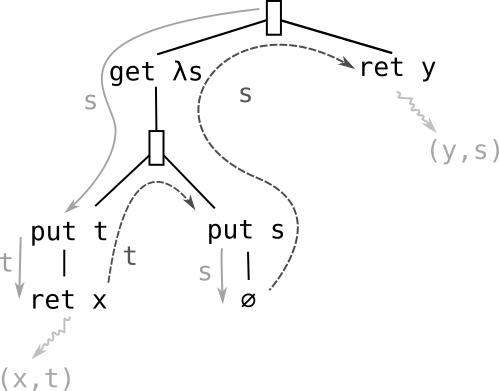
\includegraphics[scale=0.7]{sections/putR}
  \caption{Illustration of state-restoring put}
  \label{fig:putR}
\end{figure}

To help build understanding for \ensuremath{\Varid{put}_{\scaleobj{0.7}{\sf R}}}, Figure~\ref{fig:putR} shows the flow of
execution for the expression \ensuremath{(\Varid{put}_{\scaleobj{0.7}{\sf R}}\;\Varid{t}\mathbin{\hstretch{0.7}{>\!\!>}}\Varid{ret}\;\Varid{x})\mathbin{\talloblong}\Varid{ret}\;\Varid{y}}. Initially, the
state is \ensuremath{\Varid{s}}; it gets modified to \ensuremath{\Varid{t}} at the \ensuremath{\Varid{put}\;\Varid{t}} node after which the value
\ensuremath{\Varid{x}} is output with the working state \ensuremath{\Varid{t}}. Then, because we found a result, we
backtrack (since we're using global-state semantics, the state modification
caused by \ensuremath{\Varid{put}\;\Varid{t}} is not reversed), arriving in the \ensuremath{\Varid{side}} operation branch. The
\ensuremath{\Varid{put}\;\Varid{s}} operation is executed, which resets the state to \ensuremath{\Varid{s}}, and then the
branch immediately fails, so we backtrack to the right branch of the topmost
\ensuremath{(\talloblong)}. There the value \ensuremath{\Varid{y}} is output with working state \ensuremath{\Varid{s}}.

For some further intuition about \ensuremath{\Varid{put}_{\scaleobj{0.7}{\sf R}}}, consider \ensuremath{\Varid{put}_{\scaleobj{0.7}{\sf R}}\;\Varid{s}\mathbin{\hstretch{0.7}{>\!\!>}}\Varid{comp}} where \ensuremath{\Varid{comp}} is some arbitrary computation:
\begin{hscode}\SaveRestoreHook
\column{B}{@{}>{\hspre}l<{\hspost}@{}}%
\column{7}{@{}>{\hspre}l<{\hspost}@{}}%
\column{9}{@{}>{\hspre}l<{\hspost}@{}}%
\column{E}{@{}>{\hspre}l<{\hspost}@{}}%
\>[7]{}\Varid{put}_{\scaleobj{0.7}{\sf R}}\;\Varid{s}\mathbin{\hstretch{0.7}{>\!\!>}}\Varid{comp}{}\<[E]%
\\
\>[B]{}\mathbin{=}{}\<[7]%
\>[7]{}(\Varid{get}\mathrel{\hstretch{0.7}{>\!\!>\!\!=}}\lambda \Varid{s}_{0}\to \Varid{put}\;\Varid{s}\mathbin{\talloblong}\Varid{side}\;(\Varid{put}\;\Varid{s}_{0}))\mathbin{\hstretch{0.7}{>\!\!>}}\Varid{comp}{}\<[E]%
\\
\>[B]{}\mathbin{=}{}\<[9]%
\>[9]{}\mbox{\commentbegin  monad law, left-distributivity \eqref{eq:bind-mplus-dist}  \commentend}{}\<[E]%
\\
\>[B]{}\hsindent{7}{}\<[7]%
\>[7]{}\Varid{get}\mathrel{\hstretch{0.7}{>\!\!>\!\!=}}\lambda \Varid{s}_{0}\to (\Varid{put}\;\Varid{s}\mathbin{\hstretch{0.7}{>\!\!>}}\Varid{comp})\mathbin{\talloblong}(\Varid{side}\;(\Varid{put}\;\Varid{s}_{0})\mathbin{\hstretch{0.7}{>\!\!>}}\Varid{comp}){}\<[E]%
\\
\>[B]{}\mathbin{=}{}\<[9]%
\>[9]{}\mbox{\commentbegin  by \eqref{eq:bind-mzero-zero} \ensuremath{\Varid{\varnothing}\mathbin{\hstretch{0.7}{>\!\!>}}\Varid{comp}\mathrel{=}\Varid{\varnothing}}, monad laws  \commentend}{}\<[E]%
\\
\>[B]{}\hsindent{7}{}\<[7]%
\>[7]{}\Varid{get}\mathrel{\hstretch{0.7}{>\!\!>\!\!=}}\lambda \Varid{s}_{0}\to (\Varid{put}\;\Varid{s}\mathbin{\hstretch{0.7}{>\!\!>}}\Varid{comp})\mathbin{\talloblong}\Varid{side}\;(\Varid{put}\;\Varid{s}_{0})~~.{}\<[E]%
\ColumnHook
\end{hscode}\resethooks
Thanks to left-distributivity \eqref{eq:bind-mplus-dist}, \ensuremath{(\mathbin{\hstretch{0.7}{>\!\!>}}\Varid{comp})} is promoted into \ensuremath{(\talloblong)}.
Furthermore, the \ensuremath{(\mathbin{\hstretch{0.7}{>\!\!>}}\Varid{comp})} after \ensuremath{\Varid{side}\;(\Varid{put}\;\Varid{s}_{0})} is discarded by
\eqref{eq:bind-mzero-zero}.
In words, \ensuremath{\Varid{put}_{\scaleobj{0.7}{\sf R}}\;\Varid{s}\mathbin{\hstretch{0.7}{>\!\!>}}\Varid{comp}} saves the current state, computes \ensuremath{\Varid{comp}} using state \ensuremath{\Varid{s}}, and restores the saved state!
The subscript \ensuremath{\Conid{R}} stands for ``restore.''
Note also that \ensuremath{(\Varid{put}_{\scaleobj{0.7}{\sf R}}\;\Varid{s}\mathbin{\hstretch{0.7}{>\!\!>}}\Varid{m}_{1})\mathbin{\hstretch{0.7}{>\!\!>}}\Varid{m}_{2}\mathrel{=}\Varid{put}_{\scaleobj{0.7}{\sf R}}\;\Varid{s}\mathbin{\hstretch{0.7}{>\!\!>}}(\Varid{m}_{1}\mathbin{\hstretch{0.7}{>\!\!>}}\Varid{m}_{2})} --- the state restoration happens in the end.

The behaviour of \ensuremath{\Varid{put}_{\scaleobj{0.7}{\sf R}}} is rather tricky. It is instructive comparing
\begin{enumerate}[label=(\alph*)]
\item \ensuremath{\Varid{return}\;\Varid{x}},  \label{ex:putR-pitfalls-1}
\item \ensuremath{\Varid{put}\;\Varid{s}\mathbin{\hstretch{0.7}{>\!\!>}}\Varid{return}\;\Varid{x}}, \label{ex:putR-pitfalls-2}
\item \ensuremath{\Varid{put}_{\scaleobj{0.7}{\sf R}}\;\Varid{s}\mathbin{\hstretch{0.7}{>\!\!>}}\Varid{return}\;\Varid{x}}. \label{ex:putR-pitfalls-3}
\end{enumerate}
When run in initial state \ensuremath{\Varid{s}_{0}}, they all yield \ensuremath{\Varid{x}} as the result.
The final states after running \ref{ex:putR-pitfalls-1}, \ref{ex:putR-pitfalls-2} and \ref{ex:putR-pitfalls-3} are \ensuremath{\Varid{s}_{0}}, \ensuremath{\Varid{s}} and \ensuremath{\Varid{s}_{0}}, respectively.
However, \ref{ex:putR-pitfalls-3} does {\em not} behave identically to \ref{ex:putR-pitfalls-1} in all contexts!
For example, in the context \ensuremath{(\mathbin{\hstretch{0.7}{>\!\!>}}\Varid{get})}, we can tell them apart:
\ensuremath{\Varid{return}\;\Varid{x}\mathbin{\hstretch{0.7}{>\!\!>}}\Varid{get}} returns \ensuremath{\Varid{s}_{0}}, while \ensuremath{\Varid{put}_{\scaleobj{0.7}{\sf R}}\;\Varid{s}\mathbin{\hstretch{0.7}{>\!\!>}}\Varid{return}\;\Varid{x}\mathbin{\hstretch{0.7}{>\!\!>}}\Varid{get}} returns \ensuremath{\Varid{s}}, even though the program yields final state \ensuremath{\Varid{s}_{0}}.

We wish that \ensuremath{\Varid{put}_{\scaleobj{0.7}{\sf R}}}, when run with a global state, satisfies laws \eqref{eq:put-put} through \eqref{eq:mplus-bind-dist} ---
the state laws and the \emph{local} state laws.
If so, one could take a program written for a local state monad, replace all occurrences of \ensuremath{\Varid{put}} by \ensuremath{\Varid{put}_{\scaleobj{0.7}{\sf R}}}, and run the program with a global state.
Unfortunately this is not the case: \ensuremath{\Varid{put}_{\scaleobj{0.7}{\sf R}}} does satisfy {\bf put-put}~\eqref{eq:put-put} and {\bf put-get}~\eqref{eq:put-get}, but {\bf get-put}~\eqref{eq:get-put} fails ---
\ensuremath{\Varid{get}\mathrel{\hstretch{0.7}{>\!\!>\!\!=}}\Varid{put}_{\scaleobj{0.7}{\sf R}}} and \ensuremath{\Varid{return}\;()} can be
differentiated by some contexts, for example \ensuremath{(\mathbin{\hstretch{0.7}{>\!\!>}}\Varid{put}\;\Varid{t})}.
To see that, we calculate:
\begin{hscode}\SaveRestoreHook
\column{B}{@{}>{\hspre}l<{\hspost}@{}}%
\column{7}{@{}>{\hspre}l<{\hspost}@{}}%
\column{9}{@{}>{\hspre}l<{\hspost}@{}}%
\column{E}{@{}>{\hspre}l<{\hspost}@{}}%
\>[7]{}(\Varid{get}\mathrel{\hstretch{0.7}{>\!\!>\!\!=}}\Varid{put}_{\scaleobj{0.7}{\sf R}})\mathbin{\hstretch{0.7}{>\!\!>}}\Varid{put}\;\Varid{t}{}\<[E]%
\\
\>[B]{}\mathbin{=}{}\<[7]%
\>[7]{}(\Varid{get}\mathrel{\hstretch{0.7}{>\!\!>\!\!=}}\lambda \Varid{s}\to \Varid{get}\mathrel{\hstretch{0.7}{>\!\!>\!\!=}}\lambda \Varid{s}_{0}\to \Varid{put}\;\Varid{s}\mathbin{\talloblong}\Varid{side}\;(\Varid{put}\;\Varid{s}_{0}))\mathbin{\hstretch{0.7}{>\!\!>}}\Varid{put}\;\Varid{t}{}\<[E]%
\\
\>[B]{}\mathbin{=}{}\<[9]%
\>[9]{}\mbox{\commentbegin  {\bf get-get}  \commentend}{}\<[E]%
\\
\>[B]{}\hsindent{7}{}\<[7]%
\>[7]{}(\Varid{get}\mathrel{\hstretch{0.7}{>\!\!>\!\!=}}\lambda \Varid{s}\to \Varid{put}\;\Varid{s}\mathbin{\talloblong}\Varid{side}\;(\Varid{put}\;\Varid{s}))\mathbin{\hstretch{0.7}{>\!\!>}}\Varid{put}\;\Varid{t}{}\<[E]%
\\
\>[B]{}\mathbin{=}{}\<[9]%
\>[9]{}\mbox{\commentbegin  monad laws, left-distributivity  \commentend}{}\<[E]%
\\
\>[B]{}\hsindent{7}{}\<[7]%
\>[7]{}\Varid{get}\mathrel{\hstretch{0.7}{>\!\!>\!\!=}}\lambda \Varid{s}\to (\Varid{put}\;\Varid{s}\mathbin{\hstretch{0.7}{>\!\!>}}\Varid{put}\;\Varid{t})\mathbin{\talloblong}\Varid{side}\;(\Varid{put}\;\Varid{s}){}\<[E]%
\\
\>[B]{}\mathbin{=}{}\<[9]%
\>[9]{}\mbox{\commentbegin  {\bf put-put}  \commentend}{}\<[E]%
\\
\>[B]{}\hsindent{7}{}\<[7]%
\>[7]{}\Varid{get}\mathrel{\hstretch{0.7}{>\!\!>\!\!=}}\lambda \Varid{s}\to \Varid{put}\;\Varid{t}\mathbin{\talloblong}\Varid{side}\;(\Varid{put}\;\Varid{s})~~.{}\<[E]%
\ColumnHook
\end{hscode}\resethooks
Meanwhile, \ensuremath{\Varid{return}\;()\mathbin{\hstretch{0.7}{>\!\!>}}\Varid{put}\;\Varid{t}\mathrel{=}\Varid{put}\;\Varid{t}}, which does not behave in the same way as \ensuremath{\Varid{get}\mathrel{\hstretch{0.7}{>\!\!>\!\!=}}\lambda \Varid{s}\to \Varid{put}\;\Varid{t}\mathbin{\talloblong}\Varid{side}\;(\Varid{put}\;\Varid{s})} when $s \neq t$.

In a global-state setting, the left-distributivity law
\eqref{eq:bind-mplus-dist} makes it tricky to reason about combinations of
\ensuremath{(\talloblong)} and \ensuremath{(\mathrel{\hstretch{0.7}{>\!\!>\!\!=}})} operators. Suppose we have a program \ensuremath{(\Varid{m}\mathbin{\talloblong}\Varid{n})}, and we
construct an extended program by binding a continuation \ensuremath{\Varid{f}} to it such that we
get \ensuremath{(\Varid{m}\mathbin{\talloblong}\Varid{n})\mathrel{\hstretch{0.7}{>\!\!>\!\!=}}\Varid{f}} (where \ensuremath{\Varid{f}} might modify the state). Under global-state
semantics, the evaluation of the right branch is influenced by the state
modifications performed by evaluating the left branch. So by
\eqref{eq:bind-mplus-dist}, this means that when we get to evaluating the \ensuremath{\Varid{n}}
subprogram in the extended program, it will do so with a different initial state
(the one obtained after running \ensuremath{\Varid{m}\mathrel{\hstretch{0.7}{>\!\!>\!\!=}}\Varid{f}}) compared to the initial state in the
original program (the one obtained by running \ensuremath{\Varid{m}}). In other words, placing our
program in a different context changed the meaning of one of its subprograms. So
it is difficult to reason about programs compositionally in this
setting---some properties hold only when we take the entire program into
consideration.

It turns out that all properties we need do hold, provided that {\em all}
occurrences of \ensuremath{\Varid{put}} are replaced by \ensuremath{\Varid{put}_{\scaleobj{0.7}{\sf R}}}---problematic contexts such as
\ensuremath{\Varid{put}\;\Varid{t}} above are thus ruled out. However, that ``all \ensuremath{\Varid{put}} are replaced by
\ensuremath{\Varid{put}_{\scaleobj{0.7}{\sf R}}}'' is a global property, and to properly talk about it we have to formally
define contexts, which is what we will do in Section~\ref{sec:ctxt-trans}.
Notice though, that simulation of local state semantics by judicious use of
\ensuremath{\Varid{put}_{\scaleobj{0.7}{\sf R}}} does not avoid the unnecessary copying mentioned in
Section~\ref{sec:space-usage}, it merely makes it explicit in the program.
We will address this shortcoming in Section~\ref{sec:backtrack-gs}.
\section{Proving the $\mathit{put}_{\text{R}}$ Transformation Correct For a Given Implementation}
Before we tackle the general proof of correctness of the \ensuremath{\Varid{put}_{\scaleobj{0.7}{\sf R}}} transformation
correct, we dip our toes into something a bit more straightforward: showing that
the transformation is correct for specific implementations of global and local
state. This lets us use a somewhat more concrete setting to introduce some
infrastructure needed for the more general proof, as well as demonstrate a case
study of a fold fusion proof (TODO: citation), an elegant and powerful technique
that is interesting in its own right.

In the previous sections we have been mixing syntax and semantics,
which we avoid in this section by defining the program syntax as a free monad
(TODO: citation).
This way we avoid the need for a type-level distinction between programs
with local-state semantics and programs with global-state semantics.
\begin{hscode}\SaveRestoreHook
\column{B}{@{}>{\hspre}l<{\hspost}@{}}%
\column{3}{@{}>{\hspre}l<{\hspost}@{}}%
\column{7}{@{}>{\hspre}l<{\hspost}@{}}%
\column{11}{@{}>{\hspre}l<{\hspost}@{}}%
\column{15}{@{}>{\hspre}l<{\hspost}@{}}%
\column{24}{@{}>{\hspre}l<{\hspost}@{}}%
\column{E}{@{}>{\hspre}l<{\hspost}@{}}%
\>[B]{}\mathbf{data}\;\Conid{Free}\;\Varid{f}\;\Varid{a}\;\mathbf{where}{}\<[E]%
\\
\>[B]{}\hsindent{3}{}\<[3]%
\>[3]{}\Conid{Ret}\mathbin{::}\Varid{a}{}\<[24]%
\>[24]{}\to \Conid{Free}\;\Varid{f}\;\Varid{a}{}\<[E]%
\\
\>[B]{}\hsindent{3}{}\<[3]%
\>[3]{}\Conid{Op}{}\<[7]%
\>[7]{}\mathbin{::}\Varid{f}\;(\Conid{Free}\;\Varid{f}\;\Varid{a}){}\<[24]%
\>[24]{}\to \Conid{Free}\;\Varid{f}\;\Varid{a}{}\<[E]%
\\[\blanklineskip]%
\>[B]{}\mathbf{instance}\;\Conid{Functor}\;\Varid{f}\Rightarrow \Conid{Functor}\;(\Conid{Free}\;\Varid{f})\;\mathbf{where}{}\<[E]%
\\
\>[B]{}\hsindent{3}{}\<[3]%
\>[3]{}\Varid{fmap}\;\Varid{f}\;(\Conid{Ret}\;\Varid{x})\mathrel{=}\Conid{Ret}\;(\Varid{f}\;\Varid{x}){}\<[E]%
\\
\>[B]{}\hsindent{3}{}\<[3]%
\>[3]{}\Varid{fmap}\;\Varid{f}\;(\Conid{Op}\;{}\<[15]%
\>[15]{}\Varid{o})\mathrel{=}\Conid{Op}\;(\Varid{fmap}\;(\Varid{fmap}\;\Varid{f})\;\Varid{o}){}\<[E]%
\\[\blanklineskip]%
\>[B]{}\mathbf{instance}\;\Conid{Functor}\;\Varid{f}\Rightarrow \Conid{Monad}\;(\Conid{Free}\;\Varid{f})\;\mathbf{where}{}\<[E]%
\\
\>[B]{}\hsindent{3}{}\<[3]%
\>[3]{}\Varid{return}{}\<[11]%
\>[11]{}\mathrel{=}\Varid{pure}{}\<[E]%
\\
\>[B]{}\hsindent{3}{}\<[3]%
\>[3]{}\Conid{Ret}\;\Varid{x}\mathrel{\hstretch{0.7}{>\!\!>\!\!=}}\Varid{g}\mathrel{=}\Varid{g}\;\Varid{x}{}\<[E]%
\\
\>[B]{}\hsindent{3}{}\<[3]%
\>[3]{}\Conid{Op}\;\Varid{op}\mathrel{\hstretch{0.7}{>\!\!>\!\!=}}\Varid{g}\mathrel{=}\Conid{Op}\;(\Varid{fmap}\;(\mathrel{\hstretch{0.7}{>\!\!>\!\!=}}\Varid{g})\;\Varid{op}){}\<[E]%
\ColumnHook
\end{hscode}\resethooks
The state and nondeterminism interfaces are provided as ``algebras''. These are
functors equipped with a constructor for each operation they support.
\begin{hscode}\SaveRestoreHook
\column{B}{@{}>{\hspre}l<{\hspost}@{}}%
\column{3}{@{}>{\hspre}l<{\hspost}@{}}%
\column{5}{@{}>{\hspre}l<{\hspost}@{}}%
\column{12}{@{}>{\hspre}l<{\hspost}@{}}%
\column{25}{@{}>{\hspre}l<{\hspost}@{}}%
\column{E}{@{}>{\hspre}l<{\hspost}@{}}%
\>[3]{}\mathbf{data}\;\Conid{StateF}\;\Varid{a}\;\mathbf{where}{}\<[E]%
\\
\>[3]{}\hsindent{2}{}\<[5]%
\>[5]{}\Conid{Get}{}\<[12]%
\>[12]{}\mathbin{::}(\Conid{S}\to \Varid{a}){}\<[25]%
\>[25]{}\to \Conid{StateF}\;\Varid{a}{}\<[E]%
\\
\>[3]{}\hsindent{2}{}\<[5]%
\>[5]{}\Conid{Put}{}\<[12]%
\>[12]{}\mathbin{::}\Conid{S}\to \Varid{a}{}\<[25]%
\>[25]{}\to \Conid{StateF}\;\Varid{a}{}\<[E]%
\\
\>[3]{}\hsindent{2}{}\<[5]%
\>[5]{}\mathbf{deriving}\;\Conid{Functor}{}\<[E]%
\\[\blanklineskip]%
\>[3]{}\mathbf{data}\;\Conid{NondetF}\;\Varid{a}\;\mathbf{where}{}\<[E]%
\\
\>[3]{}\hsindent{2}{}\<[5]%
\>[5]{}\Varid{\varnothing}{}\<[12]%
\>[12]{}\mathbin{::}\Conid{NondetF}\;\Varid{a}{}\<[E]%
\\
\>[3]{}\hsindent{2}{}\<[5]%
\>[5]{}(\talloblong){}\<[12]%
\>[12]{}\mathbin{::}\Varid{a}\to \Varid{a}\to \Conid{NondetF}\;\Varid{a}{}\<[E]%
\\
\>[3]{}\hsindent{2}{}\<[5]%
\>[5]{}\mathbf{deriving}\;\Conid{Functor}{}\<[E]%
\ColumnHook
\end{hscode}\resethooks
In this encoding, the type \ensuremath{\Conid{Free}\;\Conid{StateF}\;\Varid{a}} represents stateful computations, and
similarly the type \ensuremath{\Conid{Free}\;\Conid{NondetF}\;\Varid{a}} represents nondeterministic computations.
Note that in this representation, our programs are written in a
continuation-passing style. For instance, where in the previous section we would
have written \ensuremath{\Varid{put}\;\Varid{t}\mathbin{\hstretch{0.7}{>\!\!>}}\Varid{get}}, we now write \ensuremath{\Conid{Op}\;(\Conid{Put}\;\Varid{t}\;(\Conid{Op}\;\Conid{Get}))}.
Computations with multiple effects can be typed with a sum type \ensuremath{(\mathbin{+})} over types
of kind \ensuremath{\mathbin{*}\to \mathbin{*}}.
\begin{hscode}\SaveRestoreHook
\column{B}{@{}>{\hspre}l<{\hspost}@{}}%
\column{3}{@{}>{\hspre}l<{\hspost}@{}}%
\column{5}{@{}>{\hspre}l<{\hspost}@{}}%
\column{E}{@{}>{\hspre}l<{\hspost}@{}}%
\>[3]{}\mathbf{data}\;(\Varid{f}\mathbin{+}\Varid{g})\;\Varid{a}\;\mathbf{where}{}\<[E]%
\\
\>[3]{}\hsindent{2}{}\<[5]%
\>[5]{}\Conid{Inl}\mathbin{::}\Varid{f}\;\Varid{a}\to (\Varid{f}\mathbin{+}\Varid{g})\;\Varid{a}{}\<[E]%
\\
\>[3]{}\hsindent{2}{}\<[5]%
\>[5]{}\Conid{Inr}\mathbin{::}\Varid{g}\;\Varid{a}\to (\Varid{f}\mathbin{+}\Varid{g})\;\Varid{a}{}\<[E]%
\\
\>[3]{}\hsindent{2}{}\<[5]%
\>[5]{}\mathbf{deriving}\;\Conid{Functor}{}\<[E]%
\ColumnHook
\end{hscode}\resethooks
The type \ensuremath{\Conid{Free}\;(\Conid{NondetF}\mathbin{+}\Conid{StateF})\;\Varid{a}} is one way to encode programs which have
both nondeterminism and state as effects. So is \ensuremath{\Conid{Free}\;(\Conid{StateF}\mathbin{+}\Conid{NondetF})\;\Varid{a}}, or
more generally \ensuremath{\Conid{Functor}\;\Varid{f}\Rightarrow \Conid{Free}\;(\Conid{StateF}\mathbin{+}(\Conid{NondetF}\mathbin{+}\Varid{f}))\;\Varid{a}} (where \ensuremath{\Varid{f}} may
introduce additional effects). 
Where in the previous section we would have written \ensuremath{\Varid{put}\;\Varid{t}\mathbin{\hstretch{0.7}{>\!\!>}}\Varid{\varnothing}}, we now
write \ensuremath{\Conid{Op}\;(\Conid{Inr}\;(\Conid{Put}\;\Varid{t}\;(\Conid{Op}\;(\Conid{Inl}\;\Varid{\varnothing}))))\mathbin{::}\Conid{Free}\;(\Conid{NondetF}\mathbin{+}\Conid{StateF})\;\Varid{a}}. We will
later introduce notation to make our syntax a bit less noisy.
The \ensuremath{(\mathbin{+})} type is morally commutative, associative, and has a zero element:
\begin{hscode}\SaveRestoreHook
\column{B}{@{}>{\hspre}l<{\hspost}@{}}%
\column{9}{@{}>{\hspre}l<{\hspost}@{}}%
\column{E}{@{}>{\hspre}l<{\hspost}@{}}%
\>[B]{}\Varid{comm}{}\<[9]%
\>[9]{}\mathbin{::}(\Conid{Functor}\;\Varid{f},\Conid{Functor}\;\Varid{g})\Rightarrow \Conid{Free}\;(\Varid{f}\mathbin{+}\Varid{g})\;\Varid{a}\to \Conid{Free}\;(\Varid{g}\mathbin{+}\Varid{f})\;\Varid{a}{}\<[E]%
\\
\>[B]{}\Varid{assocl}{}\<[9]%
\>[9]{}\mathbin{::}(\Conid{Functor}\;\Varid{f},\Conid{Functor}\;\Varid{g},\Conid{Functor}\;\Varid{h}){}\<[E]%
\\
\>[9]{}\Rightarrow \Conid{Free}\;(\Varid{f}\mathbin{+}(\Varid{g}\mathbin{+}\Varid{h}))\;\Varid{a}\to \Conid{Free}\;((\Varid{f}\mathbin{+}\Varid{g})\mathbin{+}\Varid{h})\;\Varid{a}{}\<[E]%
\\
\>[B]{}\Varid{assocr}{}\<[9]%
\>[9]{}\mathbin{::}(\Conid{Functor}\;\Varid{f},\Conid{Functor}\;\Varid{g},\Conid{Functor}\;\Varid{h}){}\<[E]%
\\
\>[9]{}\Rightarrow \Conid{Free}\;((\Varid{f}\mathbin{+}\Varid{g})\mathbin{+}\Varid{h})\;\Varid{a}\to \Conid{Free}\;(\Varid{f}\mathbin{+}(\Varid{g}\mathbin{+}\Varid{h}))\;\Varid{a}{}\<[E]%
\\[\blanklineskip]%
\>[B]{}\mathbf{data}\;\Conid{Nil}\;\Varid{a}\;\mathbf{deriving}\;\Conid{Functor}{}\<[E]%
\\[\blanklineskip]%
\>[B]{}\Varid{hNil}{}\<[9]%
\>[9]{}\mathbin{::}\Conid{Free}\;\Conid{Nil}\;\Varid{a}\to \Varid{a}{}\<[E]%
\\
\>[B]{}\Varid{hNil}\;(\Conid{Ret}\;\Varid{x})\mathrel{=}\Varid{x}{}\<[E]%
\\
\>[B]{}\mbox{\onelinecomment  other cases cannot occur}{}\<[E]%
\ColumnHook
\end{hscode}\resethooks
This zero element is an empty ``effect set'': a program of type \ensuremath{\Conid{Free}\;\Conid{Nil}\;\Varid{a}}
represents a program that computes an \ensuremath{\Varid{a}} without relying on any effects (this
type is commutative with just the type \ensuremath{\Varid{a}}).

With the \ensuremath{\Conid{Free}}-based encoding we can not only write programs
with effect sets composed from smaller effect sets, we can also write the {\em
handlers} for these effect sets compositionally.
For state and nondeterminism, we respectively write the following types for
their ``compositional'' handlers:
\begin{hscode}\SaveRestoreHook
\column{B}{@{}>{\hspre}l<{\hspost}@{}}%
\column{10}{@{}>{\hspre}l<{\hspost}@{}}%
\column{41}{@{}>{\hspre}l<{\hspost}@{}}%
\column{E}{@{}>{\hspre}l<{\hspost}@{}}%
\>[B]{}\Varid{hState}{}\<[10]%
\>[10]{}\mathbin{::}\Conid{Functor}\;\Varid{f}\Rightarrow \Conid{Free}\;(\Conid{StateF}{}\<[41]%
\>[41]{}\mathbin{+}\Varid{f})\;\Varid{a}\to (\Conid{S}\to \Conid{Free}\;\Varid{f}\;(\Varid{a},\Conid{S})){}\<[E]%
\\
\>[B]{}\Varid{hNondet}{}\<[10]%
\>[10]{}\mathbin{::}\Conid{Functor}\;\Varid{f}\Rightarrow \Conid{Free}\;(\Conid{NondetF}{}\<[41]%
\>[41]{}\mathbin{+}\Varid{f})\;\Varid{a}\to \Conid{Free}\;\Varid{f}\;(\Conid{Bag}\;\Varid{a}){}\<[E]%
\ColumnHook
\end{hscode}\resethooks
Here the \ensuremath{\Conid{Bag}} type represents a multiset data structure. We give a simple
example implementation:
\begin{hscode}\SaveRestoreHook
\column{B}{@{}>{\hspre}l<{\hspost}@{}}%
\column{3}{@{}>{\hspre}l<{\hspost}@{}}%
\column{31}{@{}>{\hspre}l<{\hspost}@{}}%
\column{53}{@{}>{\hspre}l<{\hspost}@{}}%
\column{E}{@{}>{\hspre}l<{\hspost}@{}}%
\>[3]{}\mathbf{newtype}\;\Conid{Bag}\;\Varid{a}\mathrel{=}\Conid{Bag}\;[\mskip1.5mu \Varid{a}\mskip1.5mu]\;\mathbf{deriving}\;\Conid{Functor}{}\<[E]%
\\[\blanklineskip]%
\>[3]{}\mathbf{instance}\;\Conid{Semigroup}\;(\Conid{Bag}\;\Varid{a})\;{}\<[31]%
\>[31]{}\mathbf{where}\;\Conid{Bag}\;\Varid{l}\mathbin{\Diamond}\Conid{Bag}\;\Varid{r}{}\<[53]%
\>[53]{}\mathrel{=}\Conid{Bag}\;(\Varid{l}\mathbin{+\!\!\!\!\!+}\Varid{r}){}\<[E]%
\\[\blanklineskip]%
\>[3]{}\mathbf{instance}\;\Conid{Monoid}\;(\Conid{Bag}\;\Varid{a})\;{}\<[31]%
\>[31]{}\mathbf{where}\;\Varid{mempty}{}\<[53]%
\>[53]{}\mathrel{=}\Conid{Bag}\;[\mskip1.5mu \mskip1.5mu]{}\<[E]%
\\[\blanklineskip]%
\>[3]{}\mathbf{instance}\;\Conid{Eq}\;(\Conid{Bag}\;\Varid{a})\;{}\<[31]%
\>[31]{}\mathbf{where}\;\Conid{Bag}\;\Varid{l}\doubleequals\Conid{Bag}\;\Varid{r}{}\<[53]%
\>[53]{}\mathrel{=}\Varid{sort}\;\Varid{l}\doubleequals\Varid{sort}\;\Varid{r}{}\<[E]%
\\[\blanklineskip]%
\>[3]{}\Varid{singleton}\mathbin{::}\Varid{a}\to \Conid{Bag}\;\Varid{a}{}\<[E]%
\\
\>[3]{}\Varid{singleton}\;\Varid{x}\mathrel{=}\Conid{Bag}\;[\mskip1.5mu \Varid{x}\mskip1.5mu]{}\<[E]%
\\[\blanklineskip]%
\>[3]{}\Varid{elem}\mathbin{::}\Conid{Eq}\;\Varid{a}\Rightarrow \Varid{a}\to \Conid{Bag}\;\Varid{a}\to \Conid{Int}{}\<[E]%
\\
\>[3]{}\Varid{elem}\;\Varid{x}\;(\Conid{Bag}\;\Varid{xs})\mathrel{=}\Varid{length}\;(\Varid{filter}\;(\doubleequals\Varid{x})\;\Varid{xs}){}\<[E]%
\\[\blanklineskip]%
\>[3]{}\Varid{bagFlatten}\mathbin{::}\Conid{Bag}\;(\Conid{Bag}\;\Varid{a})\to \Conid{Bag}\;\Varid{a}{}\<[E]%
\\
\>[3]{}\Varid{bagFlatten}\;(\Conid{Bag}\;\Varid{bags})\mathrel{=}\Conid{Bag}\;(\Varid{concat}\;\Varid{bags}){}\<[E]%
\ColumnHook
\end{hscode}\resethooks
The type of the \ensuremath{\Varid{hState}} and \ensuremath{\Varid{hNondet}} handlers indicate that they handle one
effect of the effect set of the program, yielding a new effectful program where
the effect set contains all the remaining effects.  This is a bit reminiscent
of a ``linked list'' of effects. Like a linked list, a ``nil'' element is
needed to terminate the list; this is provided to us by the \ensuremath{\Conid{Nil}} type.

For instance, we can compose a handler \ensuremath{\Varid{hLocal}} for local state semantics out of
the ``atomic'' handlers for state and nondeterminism.
We will only be interested in the results of the computation, not the final
states, so the final step of our local state handler is to throw away the state
information (with \ensuremath{\Varid{fmap}\;\Varid{fst}}).
\begin{hscode}\SaveRestoreHook
\column{B}{@{}>{\hspre}l<{\hspost}@{}}%
\column{10}{@{}>{\hspre}l<{\hspost}@{}}%
\column{E}{@{}>{\hspre}l<{\hspost}@{}}%
\>[B]{}\Varid{hLocal'}{}\<[10]%
\>[10]{}\mathbin{::}\Conid{Free}\;(\Conid{StateF}\mathbin{+}(\Conid{NondetF}\mathbin{+}\Conid{Nil}))\;\Varid{a}\to (\Conid{S}\to \Conid{Bag}\;(\Varid{a},\Conid{S})){}\<[E]%
\\
\>[B]{}\Varid{hLocal'}{}\<[10]%
\>[10]{}\mathrel{=}\Varid{fmap}\;(\Varid{hNil}\mathbin{\cdot}\Varid{hNondet})\mathbin{\cdot}\Varid{hState}{}\<[E]%
\\[\blanklineskip]%
\>[B]{}\Varid{hLocal}{}\<[10]%
\>[10]{}\mathbin{::}\Conid{Free}\;(\Conid{StateF}\mathbin{+}(\Conid{NondetF}\mathbin{+}\Conid{Nil}))\;\Varid{a}\to (\Conid{S}\to \Conid{Bag}\;\Varid{a}){}\<[E]%
\\
\>[B]{}\Varid{hLocal}{}\<[10]%
\>[10]{}\mathrel{=}\Varid{fmap}\;(\Varid{fmap}\;\Varid{fst})\mathbin{\cdot}\Varid{hLocal'}{}\<[E]%
\ColumnHook
\end{hscode}\resethooks
In other words, local state semantics is the semantics where we
nondeterministically choose between different stateful computations. This
matches our intuition of local state semantics: if we can picture stateful,
nondeterministic programs as trees, then local state semantics is the
interpretation of the tree where each result of the (nondeterministic, stateful)
computation corresponds to a path from root to leaf in the tree. One can compute
each of these paths entirely independently from the other paths. 
Later on, we shall prove that this composition forms a valid
implementation of local state semantics.

Global state semantics can be implemented by simply inverting the order of the
handlers: rather than nondeterministically choosing between stateful
computations as local state does, in global state semantics we'll run a
single state through a nondeterministic computation.
Just like with the local state handler, we are not interested in the final state
of the computation, only in the results, so the final step of our handler is a
\ensuremath{\Varid{fmap}\;\Varid{fst}}.
\begin{hscode}\SaveRestoreHook
\column{B}{@{}>{\hspre}l<{\hspost}@{}}%
\column{11}{@{}>{\hspre}l<{\hspost}@{}}%
\column{E}{@{}>{\hspre}l<{\hspost}@{}}%
\>[B]{}\Varid{hGlobal'}{}\<[11]%
\>[11]{}\mathbin{::}\Conid{Free}\;(\Conid{NondetF}\mathbin{+}(\Conid{StateF}\mathbin{+}\Conid{Nil}))\;\Varid{a}\to (\Conid{S}\to (\Conid{Bag}\;\Varid{a},\Conid{S})){}\<[E]%
\\
\>[B]{}\Varid{hGlobal'}{}\<[11]%
\>[11]{}\mathrel{=}\Varid{fmap}\;\Varid{hNil}\mathbin{\cdot}\Varid{hState}\mathbin{\cdot}\Varid{hNondet}{}\<[E]%
\\[\blanklineskip]%
\>[B]{}\Varid{hGlobal}{}\<[11]%
\>[11]{}\mathbin{::}\Conid{Free}\;(\Conid{NondetF}\mathbin{+}(\Conid{StateF}\mathbin{+}\Conid{Nil}))\;\Varid{a}\to (\Conid{S}\to \Conid{Bag}\;\Varid{a}){}\<[E]%
\\
\>[B]{}\Varid{hGlobal}{}\<[11]%
\>[11]{}\mathrel{=}\Varid{fmap}\;\Varid{fst}\mathbin{\cdot}\Varid{hGlobal'}{}\<[E]%
\ColumnHook
\end{hscode}\resethooks
We argue the correctness of \ensuremath{\Varid{hLocal}} and \ensuremath{\Varid{hGlobal}} (with respect to laws of
respectively local and global state semantics) in~\ref{sec:correctness-handlers}.

%From this point onwards, we will omit some technical details where confusion is
%unlikely to arise. In particular, we will omit the |Op|, |Inl| and |Inr|
%constructors from our programs. For example, when we should write
%|Op (Inl (Get (\x -> Op (Inr (p x `mplus` q x)))))| (an instance of the type
%|Free (StateF + NondetF) a|), we shall instead write
%|Get (\x -> p x `mplus` q x)|, and by this actually mean an element of the type
%|Free (StateF + NondetF) a| instead of the type |StateF (NondetF a)|.
%Moreover, in our notation the same term is also an instance of
%|Free (NondetF + StateF) a|, and of |Free| 

\subsection{Folds and Fold Fusion}
\label{sec:fold-fusion}
(TODO citations)
Rather than defining our handlers directly by writing a general recursive
function, we will write them as folds, a type of structural recursion.
\begin{hscode}\SaveRestoreHook
\column{B}{@{}>{\hspre}l<{\hspost}@{}}%
\column{3}{@{}>{\hspre}l<{\hspost}@{}}%
\column{25}{@{}>{\hspre}l<{\hspost}@{}}%
\column{E}{@{}>{\hspre}l<{\hspost}@{}}%
\>[3]{}\Varid{fold}\mathbin{::}\Conid{Functor}\;\Varid{f}\Rightarrow (\Varid{a}\to \Varid{r})\to (\Varid{f}\;\Varid{r}\to \Varid{r})\to \Conid{Free}\;\Varid{f}\;\Varid{r}\to \Varid{r}{}\<[E]%
\\
\>[3]{}\Varid{fold}\;\Varid{gen}\;\Varid{alg}\;(\Conid{Ret}\;\Varid{x}){}\<[25]%
\>[25]{}\mathrel{=}\Varid{gen}\;\Varid{x}{}\<[E]%
\\
\>[3]{}\Varid{fold}\;\Varid{gen}\;\Varid{alg}\;(\Conid{Op}\;\Varid{op}){}\<[25]%
\>[25]{}\mathrel{=}\Varid{alg}\;(\Varid{fmap}\;(\Varid{fold}\;\Varid{gen}\;\Varid{alg})\;\Varid{op}){}\<[E]%
\ColumnHook
\end{hscode}\resethooks
This more principled approach gives us more leverage when reasoning about our
programs, as certain laws hold for programs defined through fusion.
In particular, we are interested in the {\em fold fusion} law:
\begin{align*}
  \ensuremath{\Varid{h}\mathbin{\cdot}\Varid{fold}\;\Varid{gen}\;\Varid{alg}} & = \ensuremath{\Varid{fold}\;\Varid{gen'}\;\Varid{alg'}} \\
                     & \Uparrow \\
  \ensuremath{\Varid{h}\mathbin{\cdot}\Varid{gen}}          & = \ensuremath{\Varid{gen'}} \\
  \ensuremath{\Varid{h}\mathbin{\cdot}\Varid{alg}}          & = \ensuremath{\Varid{alg'}\mathbin{\cdot}\Varid{fmap}\;\Varid{h}}
\end{align*}
Informally, this law states that a post-processing step (\ensuremath{\Varid{h}}) following a fold
can, if certain conditions are met, be {\em fused} into the fold.
Moreover, it will soon become apparent that the fold fusion law is not only
helpful in proving two known programs equivalent, but in fact it can often help
in finding a fused program given a composition of two programs. This discovered
program will then be correct by construction.

We can define the state and nondeterminism handlers as folds.
\begin{hscode}\SaveRestoreHook
\column{B}{@{}>{\hspre}l<{\hspost}@{}}%
\column{3}{@{}>{\hspre}l<{\hspost}@{}}%
\column{5}{@{}>{\hspre}l<{\hspost}@{}}%
\column{32}{@{}>{\hspre}l<{\hspost}@{}}%
\column{37}{@{}>{\hspre}l<{\hspost}@{}}%
\column{E}{@{}>{\hspre}l<{\hspost}@{}}%
\>[B]{}\Varid{hState}\mathbin{::}\Conid{Functor}\;\Varid{f}\Rightarrow \Conid{Free}\;(\Conid{StateF}\mathbin{+}\Varid{f})\;\Varid{a}\to (\Conid{S}\to \Conid{Free}\;\Varid{f}\;(\Varid{a},\Conid{S})){}\<[E]%
\\
\>[B]{}\Varid{hState}\mathrel{=}\Varid{fold}\;\Varid{genState}\;\Varid{algState}{}\<[E]%
\\
\>[B]{}\hsindent{3}{}\<[3]%
\>[3]{}\mathbf{where}{}\<[E]%
\\
\>[3]{}\hsindent{2}{}\<[5]%
\>[5]{}\Varid{genState}\;\Varid{x}{}\<[32]%
\>[32]{}\mathrel{=}\lambda \Varid{s}\to \Conid{Ret}\;(\Varid{x},\Varid{s}){}\<[E]%
\\
\>[3]{}\hsindent{2}{}\<[5]%
\>[5]{}\Varid{algState}\;(\Conid{Inl}\;(\Conid{Get}\;\Varid{k})){}\<[32]%
\>[32]{}\mathrel{=}\lambda \Varid{s}\to \Varid{k}\;\Varid{s}\;\Varid{s}{}\<[E]%
\\
\>[3]{}\hsindent{2}{}\<[5]%
\>[5]{}\Varid{algState}\;(\Conid{Inl}\;(\Conid{Put}\;\Varid{t}\;\Varid{k})){}\<[32]%
\>[32]{}\mathrel{=}\lambda \anonymous \to \Varid{k}\;\Varid{t}{}\<[E]%
\\
\>[3]{}\hsindent{2}{}\<[5]%
\>[5]{}\Varid{algState}\;(\Conid{Inr}\;\Varid{p}){}\<[32]%
\>[32]{}\mathrel{=}\lambda \Varid{s}\to \Conid{Op}\;(\Varid{fmap}\;(\mathbin{\$}\Varid{s})\;\Varid{p}){}\<[E]%
\\[\blanklineskip]%
\>[B]{}\Varid{hNondet}\mathbin{::}\Conid{Functor}\;\Varid{f}\Rightarrow \Conid{Free}\;(\Conid{NondetF}\mathbin{+}\Varid{f})\;\Varid{a}\to \Conid{Free}\;\Varid{f}\;(\Conid{Bag}\;\Varid{a}){}\<[E]%
\\
\>[B]{}\Varid{hNondet}\mathrel{=}\Varid{fold}\;\Varid{genNondet}\;\Varid{algNondet}{}\<[E]%
\\
\>[B]{}\hsindent{3}{}\<[3]%
\>[3]{}\mathbf{where}{}\<[E]%
\\
\>[3]{}\hsindent{2}{}\<[5]%
\>[5]{}\Varid{genNondet}\;\Varid{x}{}\<[37]%
\>[37]{}\mathrel{=}\Conid{Ret}\;(\Varid{singleton}\;\Varid{x}){}\<[E]%
\\
\>[3]{}\hsindent{2}{}\<[5]%
\>[5]{}\Varid{algNondet}\;(\Conid{Inl}\;\Varid{\varnothing}){}\<[37]%
\>[37]{}\mathrel{=}\Conid{Ret}\;\Varid{mempty}{}\<[E]%
\\
\>[3]{}\hsindent{2}{}\<[5]%
\>[5]{}\Varid{algNondet}\;(\Conid{Inl}\;(\Varid{p}\mathbin{\talloblong}\Varid{q})){}\<[37]%
\>[37]{}\mathrel{=}(\mathbin{\Diamond})\mathrel{\raisebox{0.5\depth}{\scaleobj{0.5}{\langle}} \scaleobj{0.8}{\$} \raisebox{0.5\depth}{\scaleobj{0.5}{\rangle}}}\Varid{p}\mathrel{\raisebox{0.5\depth}{\scaleobj{0.5}{\langle}} \scaleobj{0.8}{\ast} \raisebox{0.5\depth}{\scaleobj{0.5}{\rangle}}}\Varid{q}{}\<[E]%
\\
\>[3]{}\hsindent{2}{}\<[5]%
\>[5]{}\Varid{algNondet}\;(\Conid{Inr}\;\Varid{op}){}\<[37]%
\>[37]{}\mathrel{=}\Conid{Op}\;\Varid{op}{}\<[E]%
\ColumnHook
\end{hscode}\resethooks
With our atomic handlers defined, we have also gained complete definitions for
\ensuremath{\Varid{hLocal}} and \ensuremath{\Varid{hGlobal}}, as we know how to compose them from the atomic
handlers. 

\subsubsection{A Note on Notation}
Before moving on, we will attempt to simplify our notation a bit, as it is
already becoming apparent that it's getting cumbersome, and this will
only get worse as we start reasoning with it.  For example, to write a ``get''
operator in a program typed with \ensuremath{\Conid{Free}\;(\Conid{NondetF}\mathbin{+}(\Conid{StateF}\mathbin{+}\Conid{NilF}))\;\Varid{a}} requires
us to write \ensuremath{\Conid{Inr}\;(\Conid{Inl}\;(\Conid{Op}\;(\Conid{Get}\;\Varid{k})))}. Even worse,
although we see the types 
\ensuremath{\Conid{Free}\;(\Conid{NondetF}\mathbin{+}(\Conid{StateF}\mathbin{+}\Conid{NilF}))\;\Varid{a}} and \ensuremath{\Conid{Free}\;(\Conid{StateF}\mathbin{+}(\Conid{NondetF}\mathbin{+}\Conid{NilF}))\;\Varid{a}} as
morally the same, to convert a value of one of them into the other requires some
tedious type gymnastics.
For instance, if we want \ensuremath{\Varid{hGlobal}} to operate on the same
type of programs as \ensuremath{\Varid{hLocal}}, we need to perform some intermediate transformations:
\begin{hscode}\SaveRestoreHook
\column{B}{@{}>{\hspre}l<{\hspost}@{}}%
\column{E}{@{}>{\hspre}l<{\hspost}@{}}%
\>[B]{}\Varid{hGlobal'}\mathbin{::}\Conid{Free}\;(\Conid{StateF}\mathbin{+}(\Conid{NondetF}\mathbin{+}\Conid{Nil}))\;\Varid{a}\to (\Conid{S}\to (\Conid{Bag}\;\Varid{a},\Conid{S})){}\<[E]%
\\
\>[B]{}\Varid{hGlobal'}\mathrel{=}\Varid{fmap}\;\Varid{hNil}\mathbin{\cdot}\Varid{hState}\mathbin{\cdot}\Varid{comm}\mathbin{\cdot}\Varid{hNondet}\mathbin{\cdot}\Varid{assocr}\mathbin{\cdot}\Varid{comm}{}\<[E]%
\ColumnHook
\end{hscode}\resethooks
To avoid getting bogged down in this level of technical detail, we introduce some
simplifications. From this point onwards, we assume that the type constructor
\ensuremath{(\mathbin{+})} is {\em implicitly} commutative and associative, and has \ensuremath{\Conid{Nil}} as a zero
element; for example, we treat the type
\ensuremath{\Conid{Free}\;(\Varid{f}\mathbin{+}\Varid{g}\mathbin{+}\Conid{Nil})\;\Varid{a}} as the same type as \ensuremath{\Conid{Free}\;(\Varid{g}\mathbin{+}\Varid{f})\;\Varid{a}}, without explicitly
converting between them. This includes no longer explicitly using the \ensuremath{\Varid{hNil}}
handler. We also omit the \ensuremath{\Conid{Inr}} and \ensuremath{\Conid{Inl}} constructors from our
terms when we feel it hurts legibility. So we shall write \ensuremath{\Conid{Op}\;(\Conid{Get}\;(\Conid{Op}\;(\lambda \Varid{x}\to \Varid{p}\;\Varid{x}\mathbin{\talloblong}\Varid{q}\;\Varid{x})))} to mean
\ensuremath{\Conid{Op}\;(\Conid{Inl}\;(\Conid{Get}\;(\lambda \Varid{x}\to \Conid{Op}\;(\Conid{Inr}\;(\Varid{p}\;\Varid{x}\mathbin{\talloblong}\Varid{q}\;\Varid{x})))))\mathbin{::}\Conid{Free}\;(\Conid{StateF}\mathbin{+}\Conid{NondetF})\;\Varid{a}}. 
But due to this notation it might also mean
\ensuremath{\Conid{Op}\;(\Conid{Inr}\;(\Conid{Get}\;(\lambda \Varid{x}\to \Conid{Op}\;(\Conid{Inl}\;(\Varid{p}\;\Varid{x}\mathbin{\talloblong}\Varid{q}\;\Varid{x})))))\mathbin{::}\Conid{Free}\;(\Conid{NondetF}\mathbin{+}\Conid{StateF})\;\Varid{a}},
or a term of a more complicated type like
\ensuremath{\Conid{Free}\;(\Conid{NondetF}\mathbin{+}(\Conid{StateF}\mathbin{+}\Conid{Nil}))\;\Varid{a}}. This is by design;
the type of the term will disambiguate our meaning.

The \ensuremath{\Conid{Op}} constructor is another tedious bit of notation that we have to write
over and over again every time we want to use an operator in a program. However
we feel it quickly becomes confusing if it is omitted entirely, so instead we
introduce shorthands for our operators: for instance we write \ensuremath{\Conid{Put}_\Conid{Op}\;\Varid{t}\;\Varid{k}} to mean
\ensuremath{\Conid{Op}\;(\Conid{Put}\;\Varid{t}\;\Varid{k})}, \ensuremath{\Varid{p}\mathbin{\talloblong}_\Conid{Op}\Varid{q}} to mean \ensuremath{\Conid{Op}\;(\Varid{p}\mathbin{\talloblong}\Varid{q})}, etc.

Finally, since we are primarily interested in stateful, nondeterministic
programs, we introduce a type alias for this type of program.
\begin{hscode}\SaveRestoreHook
\column{B}{@{}>{\hspre}l<{\hspost}@{}}%
\column{E}{@{}>{\hspre}l<{\hspost}@{}}%
\>[B]{}\mathbf{type}\;\Conid{Prog}\;\Varid{a}\mathrel{=}\Conid{Free}\;(\Conid{StateF}\mathbin{+}\Conid{NondetF})\;\Varid{a}{}\<[E]%
\ColumnHook
\end{hscode}\resethooks
%%%%%%%%%%%%%%%%%%%%%%%%%%%%%%%%%%%%%%%%%%%%%%%%%%%%%%%%%%%%%%%%%%%%%%%%%%%%%%%%
\subsection{The $\mathit{put}_{\text{R}}$ Transformation as a Fold}
\label{sec:trans-fold}
Our goal is to prove the \ensuremath{\Varid{put}_{\scaleobj{0.7}{\sf R}}} transformation, as introduced in
Section~\ref{sec:chaining} correct. But so far we have not even gotten around
to properly defining it!  Our representation of programs in the free monad
style allows us to express this idea directly as a fold on the type \ensuremath{\Conid{Prog}\;\Varid{a}}:
\begin{hscode}\SaveRestoreHook
\column{B}{@{}>{\hspre}l<{\hspost}@{}}%
\column{3}{@{}>{\hspre}l<{\hspost}@{}}%
\column{5}{@{}>{\hspre}l<{\hspost}@{}}%
\column{25}{@{}>{\hspre}l<{\hspost}@{}}%
\column{E}{@{}>{\hspre}l<{\hspost}@{}}%
\>[B]{}\Varid{trans}\mathbin{::}\Conid{Prog}\;\Varid{a}\to \Conid{Prog}\;\Varid{a}{}\<[E]%
\\
\>[B]{}\Varid{trans}\mathrel{=}\Varid{fold}\;\Conid{Ret}\;\Varid{algTrans}{}\<[E]%
\\
\>[B]{}\hsindent{3}{}\<[3]%
\>[3]{}\mathbf{where}{}\<[E]%
\\
\>[3]{}\hsindent{2}{}\<[5]%
\>[5]{}\Varid{algTrans}\;(\Conid{Put}\;\Varid{t}\;\Varid{k}){}\<[25]%
\>[25]{}\mathrel{=}\Conid{Get}_\Conid{Op}\;(\lambda \Varid{s}\to \Conid{Put}_\Conid{Op}\;\Varid{t}\;\Varid{k}\mathbin{\talloblong}_\Conid{Op}\Conid{Put}_\Conid{Op}\;\Varid{s}\;\Varid{\varnothing}_\Conid{Op}){}\<[E]%
\\
\>[3]{}\hsindent{2}{}\<[5]%
\>[5]{}\Varid{algTrans}\;\Varid{p}{}\<[25]%
\>[25]{}\mathrel{=}\Conid{Op}\;\Varid{p}{}\<[E]%
\ColumnHook
\end{hscode}\resethooks
What would it mean for \ensuremath{\Varid{trans}} to be ``correct''? Our informal problem
statement was that it should ``transform between local state and global
state semantics''. In other words, running a program \ensuremath{\Varid{p}} under local state
semantics should always produce the exact same result as running the program
\ensuremath{\Varid{trans}\;\Varid{p}} under global state semantics:
\begin{hscode}\SaveRestoreHook
\column{B}{@{}>{\hspre}l<{\hspost}@{}}%
\column{E}{@{}>{\hspre}l<{\hspost}@{}}%
\>[B]{}\Varid{hGlobal}\mathbin{\cdot}\Varid{trans}\mathrel{=}\Varid{hLocal}{}\<[E]%
\ColumnHook
\end{hscode}\resethooks
If we can prove that this equation holds, then we have proven \ensuremath{\Varid{trans}} correct,
at least with respect to the specific implementations of local and global
state given in this section.
The core insight of our proof is that this equation can be proven through
fold fusion: \ensuremath{\Varid{trans}} itself is defined as a fold; \ensuremath{\Varid{hLocal}} is not defined as a
single fold, but we can fuse the local state handler into a single fold.
\begin{hscode}\SaveRestoreHook
\column{B}{@{}>{\hspre}l<{\hspost}@{}}%
\column{E}{@{}>{\hspre}l<{\hspost}@{}}%
\>[B]{}\Varid{hGlobal}\mathbin{\cdot}\Varid{fold}\;\Conid{Ret}\;\Varid{algTrans}\mathrel{=}\Varid{fold}\;\Varid{genLocal}\;\Varid{algLocal}{}\<[E]%
\ColumnHook
\end{hscode}\resethooks
In other words, we wish to show that local state semantics can be obtained by
fusing a global state ``postprocessing step'' into the \ensuremath{\Varid{trans}} fold.
Proving this equation then becomes as simple as proving the corresponding fusion
conditions:
\begin{hscode}\SaveRestoreHook
\column{B}{@{}>{\hspre}l<{\hspost}@{}}%
\column{30}{@{}>{\hspre}l<{\hspost}@{}}%
\column{E}{@{}>{\hspre}l<{\hspost}@{}}%
\>[B]{}\Varid{hGlobal}\mathbin{\cdot}\Conid{Ret}{}\<[30]%
\>[30]{}\mathrel{=}\Varid{genLocal}{}\<[E]%
\\
\>[B]{}\Varid{hGlobal}\mathbin{\cdot}\Varid{algTrans}{}\<[30]%
\>[30]{}\mathrel{=}\Varid{algLocal}\mathbin{\cdot}\Varid{fmap}\;\Varid{hGlobal}{}\<[E]%
\ColumnHook
\end{hscode}\resethooks

\subsection{Fusing the Local State Handler}
Our first step then is to find implementations for \ensuremath{\Varid{genLocal}} and \ensuremath{\Varid{algLocal}},
which we do by using fold fusion on \ensuremath{\Varid{hLocal}}.
Recall the (unfolded) definition of \ensuremath{\Varid{hLocal}}:
\begin{hscode}\SaveRestoreHook
\column{B}{@{}>{\hspre}l<{\hspost}@{}}%
\column{E}{@{}>{\hspre}l<{\hspost}@{}}%
\>[B]{}\Varid{hLocal}\mathbin{::}\Conid{Free}\;(\Conid{StateF}\mathbin{+}(\Conid{NondetF}\mathbin{+}\Conid{Nil}))\;\Varid{a}\to (\Conid{S}\to \Conid{Bag}\;\Varid{a}){}\<[E]%
\\
\>[B]{}\Varid{hLocal}\mathrel{=}\Varid{fmap}\;(\Varid{fmap}\;\Varid{fst})\mathbin{\cdot}\Varid{fmap}\;(\Varid{hNil}\mathbin{\cdot}\Varid{hNondet})\mathbin{\cdot}\Varid{hState}{}\<[E]%
\ColumnHook
\end{hscode}\resethooks
We apply the simplifications described earlier (and the functor law
\ensuremath{\Varid{fmap}\;\Varid{f}\mathbin{\cdot}\Varid{fmap}\;\Varid{g}\mathrel{=}\Varid{fmap}\;(\Varid{f}\mathbin{\cdot}\Varid{g})}) to rewrite as:
\begin{hscode}\SaveRestoreHook
\column{B}{@{}>{\hspre}l<{\hspost}@{}}%
\column{9}{@{}>{\hspre}l<{\hspost}@{}}%
\column{E}{@{}>{\hspre}l<{\hspost}@{}}%
\>[B]{}\Varid{hLocal}{}\<[9]%
\>[9]{}\mathbin{::}\Conid{Prog}\;\Varid{a}\to (\Conid{S}\to \Conid{Bag}\;\Varid{a}){}\<[E]%
\\
\>[B]{}\Varid{hLocal}{}\<[9]%
\>[9]{}\mathrel{=}\Varid{fmap}\;(\Varid{fmap}\;\Varid{fst})\mathbin{\cdot}\Varid{fmap}\;\Varid{hNondet}\mathbin{\cdot}\Varid{hState}{}\<[E]%
\\
\>[9]{}\mathrel{=}\Varid{fmap}\;(\Varid{fmap}\;\Varid{fst}\mathbin{\cdot}\Varid{hNondet})\mathbin{\cdot}\Varid{fold}\;\Varid{genState}\;\Varid{algState}{}\<[E]%
\ColumnHook
\end{hscode}\resethooks
We also abbreviate the postprocessing step:
\begin{hscode}\SaveRestoreHook
\column{B}{@{}>{\hspre}l<{\hspost}@{}}%
\column{E}{@{}>{\hspre}l<{\hspost}@{}}%
\>[B]{}\Varid{post}\mathrel{=}\Varid{fmap}\;\Varid{fst}\mathbin{\cdot}\Varid{hNondet}{}\<[E]%
\ColumnHook
\end{hscode}\resethooks
Then our fold fusion problem statement becomes
\begin{align*}
  \ensuremath{\Varid{fmap}\;\Varid{post}\mathbin{\cdot}\Varid{fold}\;\Varid{genState}\;\Varid{algState}} & = \ensuremath{\Varid{fold}\;\Varid{genLocal}\;\Varid{algLocal}} \\
                     & \Uparrow \\
  \ensuremath{\Varid{fmap}\;\Varid{post}\mathbin{\cdot}\Varid{genState}}          & = \ensuremath{\Varid{genLocal}} \\
  \ensuremath{\Varid{fmap}\;\Varid{post}\mathbin{\cdot}\Varid{algState}}          & = \ensuremath{\Varid{algLocal}\mathbin{\cdot}\Varid{fmap}\;(\Varid{fmap}\;\Varid{post})}
\end{align*}
We follow this trail to discover definitions for \ensuremath{\Varid{genLocal}} and \ensuremath{\Varid{algLocal}}.
Finding the definition of \ensuremath{\Varid{genLocal}} is merely a matter of unfolding definitions.
\begin{hscode}\SaveRestoreHook
\column{B}{@{}>{\hspre}l<{\hspost}@{}}%
\column{E}{@{}>{\hspre}l<{\hspost}@{}}%
\>[B]{}\Varid{genLocal}\mathrel{=}\Varid{fmap}\;\Varid{post}\mathbin{\cdot}\Varid{genState}{}\<[E]%
\\
\>[B]{}\mathbin{=}\mbox{\commentbegin  unfold \ensuremath{\Varid{post}}  \commentend}{}\<[E]%
\\
\>[B]{}\Varid{genLocal}\mathrel{=}\Varid{fmap}\;(\Varid{fmap}\;\Varid{fst}\mathbin{\cdot}\Varid{hNondet})\mathbin{\cdot}\Varid{genState}{}\<[E]%
\\
\>[B]{}\mathbin{=}\mbox{\commentbegin  unfold \ensuremath{\Varid{hNondet}}, \ensuremath{\Varid{genState}}  \commentend}{}\<[E]%
\\
\>[B]{}\Varid{genLocal}\mathrel{=}\Varid{fmap}\;(\Varid{fmap}\;\Varid{fst}\mathbin{\cdot}\Varid{fold}\;\Varid{genNondet}\;\Varid{algNondet})\mathbin{\cdot}(\lambda \Varid{x}\;\Varid{s}\to \Conid{Ret}\;(\Varid{x},\Varid{s})){}\<[E]%
\\
\>[B]{}\mathbin{=}\mbox{\commentbegin  unfold \ensuremath{(\mathbin{\cdot})}, \ensuremath{\Varid{fmap}}, \ensuremath{\Varid{fold}}  \commentend}{}\<[E]%
\\
\>[B]{}\Varid{genLocal}\mathrel{=}\lambda \Varid{x}\;\Varid{s}\to \Varid{fmap}\;\Varid{fst}\;(\Varid{genNondet}\;(\Conid{Ret}\;(\Varid{x},\Varid{s}))){}\<[E]%
\\
\>[B]{}\mathbin{=}\mbox{\commentbegin  unfold \ensuremath{\Varid{genNondet}}, \ensuremath{\Varid{fmap}\;\Varid{fst}}  \commentend}{}\<[E]%
\\
\>[B]{}\Varid{genLocal}\mathrel{=}\lambda \Varid{x}\;\anonymous \to \Varid{singleton}\;\Varid{x}{}\<[E]%
\ColumnHook
\end{hscode}\resethooks
Finding \ensuremath{\Varid{algLocal}} is a bit more work. We would like to transform the equation
\ensuremath{\Varid{fmap}\;(\Varid{fmap}\;\Varid{fst}\mathbin{\cdot}\Varid{hNondet})\mathbin{\cdot}\Varid{algState}\mathrel{=}\Varid{algLocal}\mathbin{\cdot}\Varid{fmap}\;(\Varid{fmap}\;(\Varid{fmap}\;\Varid{fst}\mathbin{\cdot}\Varid{hNondet}))} into an equation of the form \ensuremath{\Varid{algLocal}\;\Varid{m}\mathrel{=}\mathbin{?}}. We'll do this by
``pattern matching'' on \ensuremath{\Varid{m}}, that is, we will look for a matching right hand
side for each of the following equations.
\begin{hscode}\SaveRestoreHook
\column{B}{@{}>{\hspre}l<{\hspost}@{}}%
\column{25}{@{}>{\hspre}l<{\hspost}@{}}%
\column{E}{@{}>{\hspre}l<{\hspost}@{}}%
\>[B]{}\Varid{algLocal}\;(\Conid{Put}\;\Varid{t}\;\Varid{k}){}\<[25]%
\>[25]{}\mathrel{=}\mathbin{?}{}\<[E]%
\\
\>[B]{}\Varid{algLocal}\;(\Conid{Get}\;\Varid{k}){}\<[25]%
\>[25]{}\mathrel{=}\mathbin{?}{}\<[E]%
\\
\>[B]{}\Varid{algLocal}\;\Varid{\varnothing}{}\<[25]%
\>[25]{}\mathrel{=}\mathbin{?}{}\<[E]%
\\
\>[B]{}\Varid{algLocal}\;(\Varid{p}\mathbin{\talloblong}\Varid{q}){}\<[25]%
\>[25]{}\mathrel{=}\mathbin{?}{}\<[E]%
\ColumnHook
\end{hscode}\resethooks
We begin by applying both sides of the equation to an arbitrary argument, and
then proceed by case analysis on that argument.
\begin{hscode}\SaveRestoreHook
\column{B}{@{}>{\hspre}l<{\hspost}@{}}%
\column{E}{@{}>{\hspre}l<{\hspost}@{}}%
\>[B]{}\Varid{fmap}\;\Varid{post}\mathbin{\cdot}\Varid{algState}\mathrel{=}\Varid{algLocal}\mathbin{\cdot}\Varid{fmap}\;(\Varid{fmap}\;\Varid{post}){}\<[E]%
\\
\>[B]{}\mathbin{=}\mbox{\commentbegin  apply both sides to \ensuremath{\Varid{m}}, unfold \ensuremath{(\mathbin{\cdot})}  \commentend}{}\<[E]%
\\
\>[B]{}\Varid{fmap}\;\Varid{post}\;(\Varid{algState}\;\Varid{m})\mathrel{=}\Varid{algLocal}\;(\Varid{fmap}\;(\Varid{fmap}\;\Varid{post})\;\Varid{m}){}\<[E]%
\ColumnHook
\end{hscode}\resethooks
First, we analyze the case \ensuremath{\Varid{m}\mathrel{=}\Conid{Put}\;\Varid{t}\;\Varid{k}}. The general pattern of this case will
repeat in all other cases: first we unfold definitions, which yields an
application of \ensuremath{\Varid{algLocal}} to a term that is too specific, so we look for a way to
generalize the equation.
\begin{hscode}\SaveRestoreHook
\column{B}{@{}>{\hspre}l<{\hspost}@{}}%
\column{E}{@{}>{\hspre}l<{\hspost}@{}}%
\>[B]{}\Varid{fmap}\;\Varid{post}\;(\Varid{algState}\;(\Conid{Put}\;\Varid{t}\;\Varid{k}))\mathrel{=}\Varid{algLocal}\;(\Varid{fmap}\;(\Varid{fmap}\;\Varid{post})\;(\Conid{Put}\;\Varid{t}\;\Varid{k})){}\<[E]%
\\
\>[B]{}\mathbin{=}\mbox{\commentbegin  unfold \ensuremath{\Varid{algState}}, \ensuremath{\Varid{fmap}}  \commentend}{}\<[E]%
\\
\>[B]{}\Varid{fmap}\;\Varid{post}\;(\lambda \anonymous \to \Varid{k}\;\Varid{t})\mathrel{=}\Varid{algLocal}\;(\Conid{Put}\;\Varid{t}\;(\Varid{fmap}\;\Varid{post}\;\Varid{k})){}\<[E]%
\\
\>[B]{}\mathbin{=}\mbox{\commentbegin  unfold \ensuremath{\Varid{fmap}}  \commentend}{}\<[E]%
\\
\>[B]{}\Varid{post}\mathbin{\cdot}(\lambda \anonymous \to \Varid{k}\;\Varid{t})\mathrel{=}\Varid{algLocal}\;(\Conid{Put}\;\Varid{t}\;(\Varid{post}\mathbin{\cdot}\Varid{k})){}\<[E]%
\\
\>[B]{}\mathbin{=}\mbox{\commentbegin  definition of \ensuremath{(\mathbin{\cdot})}  \commentend}{}\<[E]%
\\
\>[B]{}\lambda \anonymous \to (\Varid{post}\mathbin{\cdot}\Varid{k})\;\Varid{t}\mathrel{=}\Varid{algLocal}\;(\Conid{Put}\;\Varid{t}\;(\Varid{post}\mathbin{\cdot}\Varid{k})){}\<[E]%
\\
\>[B]{}\mathbin{=}\mbox{\commentbegin  generalize \ensuremath{\Varid{post}\mathbin{\cdot}\Varid{k}} as \ensuremath{\Varid{k'}}  \commentend}{}\<[E]%
\\
\>[B]{}\lambda \anonymous \to \Varid{k'}\;\Varid{t}\mathrel{=}\Varid{algLocal}\;(\Conid{Put}\;\Varid{t}\;\Varid{k'}){}\<[E]%
\ColumnHook
\end{hscode}\resethooks
Initially the argument to \ensuremath{\Varid{algLocal}}, \ensuremath{\Conid{Put}\;\Varid{t}\;(\Varid{post}\mathbin{\cdot}\Varid{k})}, is too
specific to cover all cases, so we massage the other side of the equation until
\ensuremath{\Varid{post}\mathbin{\cdot}\Varid{k}} occurs there too, so we can generalize both sides. The cases \ensuremath{\Varid{m}\mathrel{=}\Conid{Get}\;\Varid{k}} and \ensuremath{\Varid{m}\mathrel{=}\Varid{p}\mathbin{\talloblong}\Varid{q}} proceed quite similarly.
\begin{hscode}\SaveRestoreHook
\column{B}{@{}>{\hspre}l<{\hspost}@{}}%
\column{E}{@{}>{\hspre}l<{\hspost}@{}}%
\>[B]{}\Varid{fmap}\;\Varid{post}\;(\Varid{algState}\;(\Conid{Get}\;\Varid{k}))\mathrel{=}\Varid{algLocal}\;(\Varid{fmap}\;(\Varid{fmap}\;\Varid{post})\;(\Conid{Get}\;\Varid{k})){}\<[E]%
\\
\>[B]{}\mathbin{=}\mbox{\commentbegin  definition of \ensuremath{\Varid{algState}}, \ensuremath{\Varid{fmap}}  \commentend}{}\<[E]%
\\
\>[B]{}\Varid{fmap}\;\Varid{post}\;(\lambda \Varid{s}\to \Varid{k}\;\Varid{s}\;\Varid{s})\mathrel{=}\Varid{algLocal}\;(\Conid{Get}\;(\lambda \Varid{s}\to \Varid{fmap}\;\Varid{post}\mathbin{\cdot}\Varid{k})){}\<[E]%
\\
\>[B]{}\mathbin{=}\mbox{\commentbegin  definition of \ensuremath{(\mathbin{\cdot})}, \ensuremath{\Varid{fmap}}  \commentend}{}\<[E]%
\\
\>[B]{}\lambda \Varid{s}\to (\Varid{post}\mathbin{\cdot}\Varid{k}\;\Varid{s})\;\Varid{s}\mathrel{=}\Varid{algLocal}\;(\Conid{Get}\;(\lambda \Varid{s}\to \Varid{post}\mathbin{\cdot}\Varid{k}\;\Varid{s})){}\<[E]%
\\
\>[B]{}\mathbin{=}\mbox{\commentbegin  $\eta$-expansion on LHS, $\alpha$-renaming on RHS  \commentend}{}\<[E]%
\\
\>[B]{}\lambda \Varid{s}\to ((\lambda \Varid{t}\to \Varid{post}\mathbin{\cdot}\Varid{k}\;\Varid{t})\;\Varid{s})\;\Varid{s}\mathrel{=}\Varid{algLocal}\;(\Conid{Get}\;(\lambda \Varid{t}\to \Varid{post}\mathbin{\cdot}\Varid{k}\;\Varid{t})){}\<[E]%
\\
\>[B]{}\mathbin{=}\mbox{\commentbegin  generalize \ensuremath{(\lambda \Varid{t}\to \Varid{post}\mathbin{\cdot}\Varid{k}\;\Varid{t})} as \ensuremath{\Varid{k'}}  \commentend}{}\<[E]%
\\
\>[B]{}\lambda \Varid{s}\to \Varid{k'}\;\Varid{s}\;\Varid{s}\mathrel{=}\Varid{algLocal}\;(\Conid{Get}\;\Varid{k'}){}\<[E]%
\ColumnHook
\end{hscode}\resethooks
%fmap hNondet (\s -> Op (p s `mplus` q s)) = algLocal (fmap hNondet p `mplus` fmap hNondet q)
%\s -> hNondet (Op (p s `mplus` q s)) = algLocal (hNondet . p `mplus` hNondet . q)
%\s -> hNondet (Op (p s `mplus` q s)) = algLocal (hNondet . p `mplus` hNondet . q)
%\s -> algNondet (fmap hNondet (p s `mplus` q s)) = algLocal (hNondet . p `mplus` hNondet . q)
%\s -> algNondet (hNondet (p s) `mplus` hNondet (q s)) = algLocal (hNondet . p `mplus` hNondet . q)
\begin{hscode}\SaveRestoreHook
\column{B}{@{}>{\hspre}l<{\hspost}@{}}%
\column{E}{@{}>{\hspre}l<{\hspost}@{}}%
\>[B]{}\Varid{fmap}\;\Varid{post}\;(\Varid{algState}\;(\Varid{p}\mathbin{\talloblong}\Varid{q}))\mathrel{=}\Varid{algLocal}\;(\Varid{fmap}\;(\Varid{fmap}\;\Varid{post})\;(\Varid{p}\mathbin{\talloblong}\Varid{q})){}\<[E]%
\\
\>[B]{}\mathbin{=}\mbox{\commentbegin  definition \ensuremath{\Varid{algState}}, \ensuremath{\Varid{fmap}}  \commentend}{}\<[E]%
\\
\>[B]{}\Varid{fmap}\;\Varid{post}\;(\lambda \Varid{s}\to \Conid{Op}\;(\Varid{p}\;\Varid{s}\mathbin{\talloblong}\Varid{q}\;\Varid{s}))\mathrel{=}\Varid{algLocal}\;(\Varid{fmap}\;\Varid{post}\;\Varid{p}\mathbin{\talloblong}\Varid{fmap}\;\Varid{post}\;\Varid{q}){}\<[E]%
\\
\>[B]{}\mathbin{=}\mbox{\commentbegin  definition of \ensuremath{\Varid{fmap}}, \ensuremath{\Varid{post}}  \commentend}{}\<[E]%
\\
\>[B]{}\lambda \Varid{s}\to \Varid{fmap}\;\Varid{fst}\;(\Varid{hNondet}\;(\Conid{Op}\;(\Varid{p}\;\Varid{s}\mathbin{\talloblong}\Varid{q}\;\Varid{s})))\mathrel{=}\Varid{algLocal}\;(\Varid{post}\mathbin{\cdot}\Varid{p}\mathbin{\talloblong}\Varid{post}\mathbin{\cdot}\Varid{q}){}\<[E]%
\\
\>[B]{}\mathbin{=}\mbox{\commentbegin  definition of \ensuremath{\Varid{hNondet}}  \commentend}{}\<[E]%
\\
\>[B]{}\lambda \Varid{s}\to \Varid{fmap}\;\Varid{fst}\;((\Varid{hNondet}\mathbin{\cdot}\Varid{p})\;\Varid{s}\mathbin{\Diamond}(\Varid{hNondet}\mathbin{\cdot}\Varid{q})\;\Varid{s})\mathrel{=}\Varid{algLocal}\;(\Varid{post}\mathbin{\cdot}\Varid{p}\mathbin{\talloblong}\Varid{post}\mathbin{\cdot}\Varid{q}){}\<[E]%
\\
\>[B]{}\mathbin{=}\mbox{\commentbegin  \ensuremath{\Varid{map}} distributes over \ensuremath{(\mathbin{\Diamond})} (proof left as exercise), definition of \ensuremath{\Varid{post}}  \commentend}{}\<[E]%
\\
\>[B]{}\lambda \Varid{s}\to (\Varid{post}\mathbin{\cdot}\Varid{p})\;\Varid{s}\mathbin{\Diamond}(\Varid{post}\mathbin{\cdot}\Varid{q})\;\Varid{s}\mathrel{=}\Varid{algLocal}\;(\Varid{post}\mathbin{\cdot}\Varid{p}\mathbin{\talloblong}\Varid{post}\mathbin{\cdot}\Varid{q}){}\<[E]%
\\
\>[B]{}\mathbin{=}\mbox{\commentbegin  generalize \ensuremath{\Varid{post}\mathbin{\cdot}\Varid{p}} as \ensuremath{\Varid{p'}} and \ensuremath{\Varid{post}\mathbin{\cdot}\Varid{q}} as \ensuremath{\Varid{q'}}  \commentend}{}\<[E]%
\\
\>[B]{}\lambda \Varid{s}\to \Varid{p'}\;\Varid{s}\mathbin{\Diamond}\Varid{q'}\;\Varid{s}\mathrel{=}\Varid{algLocal}\;(\Varid{p'}\mathbin{\talloblong}\Varid{q'}){}\<[E]%
\ColumnHook
\end{hscode}\resethooks
%\s -> algNondet ((fmap fst . hNondet . p) s `mplus` (fmap fst . hNondet . q) s) = algLocal (fmap fst . hNondet . p `mplus` fmap fst . hNondet . q)
%=== {- generalize |fmap fst . hNondet . p| as |p'| and |fmap fst . hNondet . q| as |q'| -}
%\s -> algNondet (p' s `mplus` q' s) = algLocal (p' `mplus` q')
%=== {-  -}
%\s -> p' s <> q' s = algLocal (p' `mplus` q')
Finally, the case for \ensuremath{\Varid{m}\mathrel{=}\Conid{Fail}} is trivial. We find \ensuremath{\Varid{algLocal}\;\Conid{Fail}\mathrel{=}\lambda \anonymous \to \Varid{mempty}}. In summary, we deduced the following implementation for \ensuremath{\Varid{algLocal}}:
\begin{hscode}\SaveRestoreHook
\column{B}{@{}>{\hspre}l<{\hspost}@{}}%
\column{25}{@{}>{\hspre}l<{\hspost}@{}}%
\column{E}{@{}>{\hspre}l<{\hspost}@{}}%
\>[B]{}\Varid{algLocal}\;(\Conid{Put}\;\Varid{t}\;\Varid{k}){}\<[25]%
\>[25]{}\mathrel{=}\lambda \anonymous \to \Varid{k}\;\Varid{t}{}\<[E]%
\\
\>[B]{}\Varid{algLocal}\;(\Conid{Get}\;\Varid{k}){}\<[25]%
\>[25]{}\mathrel{=}\lambda \Varid{s}\to \Varid{k}\;\Varid{s}\;\Varid{s}{}\<[E]%
\\
\>[B]{}\Varid{algLocal}\;\Varid{\varnothing}{}\<[25]%
\>[25]{}\mathrel{=}\lambda \anonymous \to \Varid{mempty}{}\<[E]%
\\
\>[B]{}\Varid{algLocal}\;(\Varid{p}\mathbin{\talloblong}\Varid{q}){}\<[25]%
\>[25]{}\mathrel{=}\lambda \Varid{s}\to \Varid{p}\;\Varid{s}\mathbin{\Diamond}\Varid{q}\;\Varid{s}{}\<[E]%
\ColumnHook
\end{hscode}\resethooks

Finding our fused local state handler was the last challenge in proving \ensuremath{\Varid{trans}}
correct. All that remains to be done is to prove that the fusion conditions hold:
\begin{hscode}\SaveRestoreHook
\column{B}{@{}>{\hspre}l<{\hspost}@{}}%
\column{30}{@{}>{\hspre}l<{\hspost}@{}}%
\column{E}{@{}>{\hspre}l<{\hspost}@{}}%
\>[B]{}\Varid{hGlobal}\mathbin{\cdot}\Conid{Ret}{}\<[30]%
\>[30]{}\mathrel{=}\Varid{genLocal}{}\<[E]%
\\
\>[B]{}\Varid{hGlobal}\mathbin{\cdot}\Varid{algTrans}{}\<[30]%
\>[30]{}\mathrel{=}\Varid{algLocal}\mathbin{\cdot}\Varid{fmap}\;\Varid{hGlobal}{}\<[E]%
\ColumnHook
\end{hscode}\resethooks
But this proof is entirely trivial. Since there are no unknowns, it is merely a
matter of fully evaluating (after pattern matching) both sides of the equation
and verifying that they produce the same value.

\subsection{Correctness of \ensuremath{\Varid{hLocal}} and \ensuremath{\Varid{hGlobal}}}
\label{sec:correctness-handlers}
The preceding proof rests on the assumption that \ensuremath{\Varid{hLocal}} correctly implements
local state semantics. By that we mean that \ensuremath{\Varid{hLocal}} respects the state,
nondeterminism and local state laws. To give an example, it must be the case
that, for all program contexts \ensuremath{\Conid{C}},
\ensuremath{\Varid{hLocal}\;\Conid{C}\;[\mskip1.5mu \Varid{put}\;\Varid{s}\mathbin{\hstretch{0.7}{>\!\!>}}\Varid{put}\;\Varid{t}\mskip1.5mu]\mathrel{=}\Varid{hLocal}\;\Conid{C}\;[\mskip1.5mu \Varid{put}\;\Varid{t}\mskip1.5mu]}. A program context can be seen as a
``program with a hole'', writing \ensuremath{\Conid{C}\;[\mskip1.5mu \Varid{p}\mskip1.5mu]} means filling in the program \ensuremath{\Varid{p}} into
the context \ensuremath{\Conid{C}}. We elaborate on this concept in~\ref{sec:contextual-equivalence}.
To understand why the handler is, indeed, correct, consider that \ensuremath{\Varid{hLocal'}} is a
homomorphism (a transformation between algebraic structures that preserves
structure) in the algebra defined by the interface of \ensuremath{\Conid{MStateNondet}}. That is,
the algebra is a type constructor \ensuremath{\Varid{m}\mathbin{::}\mathbin{*}\to \mathbin{*}} along with implementations for
\ensuremath{\Varid{return}}, \ensuremath{(\mathrel{\hstretch{0.7}{>\!\!>\!\!=}})}, \ensuremath{\Varid{get}}, \ensuremath{\Varid{put}}, \ensuremath{\Varid{\varnothing}}, \ensuremath{(\talloblong)}.
One instance of this algebra is the \ensuremath{\Conid{Prog}} type:
\begin{hscode}\SaveRestoreHook
\column{B}{@{}>{\hspre}l<{\hspost}@{}}%
\column{3}{@{}>{\hspre}l<{\hspost}@{}}%
\column{5}{@{}>{\hspre}l<{\hspost}@{}}%
\column{12}{@{}>{\hspre}l<{\hspost}@{}}%
\column{18}{@{}>{\hspre}l<{\hspost}@{}}%
\column{E}{@{}>{\hspre}l<{\hspost}@{}}%
\>[3]{}\mathbf{instance}\;\Conid{MState}\;\Conid{S}\;\Conid{Prog}\;\mathbf{where}{}\<[E]%
\\
\>[3]{}\hsindent{2}{}\<[5]%
\>[5]{}\Varid{put}\;\Varid{t}{}\<[12]%
\>[12]{}\mathrel{=}\Conid{Put}_\Conid{Op}\;\Varid{t}\;(\Conid{Ret}\;()){}\<[E]%
\\
\>[3]{}\hsindent{2}{}\<[5]%
\>[5]{}\Varid{get}{}\<[12]%
\>[12]{}\mathrel{=}\Conid{Get}_\Conid{Op}\;\Conid{Ret}{}\<[E]%
\\[\blanklineskip]%
\>[3]{}\mathbf{instance}\;\Conid{MNondet}\;\Conid{Prog}\;\mathbf{where}{}\<[E]%
\\
\>[3]{}\hsindent{2}{}\<[5]%
\>[5]{}\Varid{\varnothing}{}\<[18]%
\>[18]{}\mathrel{=}\Varid{\varnothing}_\Conid{Op}{}\<[E]%
\\
\>[3]{}\hsindent{2}{}\<[5]%
\>[5]{}\Varid{p}\mathbin{\talloblong}\Varid{q}{}\<[18]%
\>[18]{}\mathrel{=}\Varid{p}\mathbin{\talloblong}_\Conid{Op}\Varid{q}{}\<[E]%
\\[\blanklineskip]%
\>[3]{}\mathbf{instance}\;\Conid{MStateNondet}\;\Conid{S}\;\Conid{Prog}{}\<[E]%
\ColumnHook
\end{hscode}\resethooks
The semantic domain of the local state handler \ensuremath{\Varid{hNondet'}} is also an instance of
this algebra.
\begin{hscode}\SaveRestoreHook
\column{B}{@{}>{\hspre}l<{\hspost}@{}}%
\column{3}{@{}>{\hspre}l<{\hspost}@{}}%
\column{5}{@{}>{\hspre}l<{\hspost}@{}}%
\column{7}{@{}>{\hspre}l<{\hspost}@{}}%
\column{12}{@{}>{\hspre}l<{\hspost}@{}}%
\column{15}{@{}>{\hspre}l<{\hspost}@{}}%
\column{18}{@{}>{\hspre}l<{\hspost}@{}}%
\column{46}{@{}>{\hspre}l<{\hspost}@{}}%
\column{E}{@{}>{\hspre}l<{\hspost}@{}}%
\>[3]{}\mathbf{newtype}\;\Conid{Dom}_\Conid{L}\;\Varid{a}\mathrel{=}\Conid{Dom}_\Conid{L}\;\{\mskip1.5mu \Varid{unDom}_\Conid{L}\mathbin{::}\Conid{S}\to \Conid{Bag}\;(\Varid{a},\Conid{S})\mskip1.5mu\}{}\<[E]%
\\[\blanklineskip]%
\>[3]{}\mathbf{instance}\;\Conid{Monad}\;\Conid{Dom}_\Conid{L}\;\mathbf{where}{}\<[E]%
\\
\>[3]{}\hsindent{2}{}\<[5]%
\>[5]{}\Varid{return}\;\Varid{x}{}\<[15]%
\>[15]{}\mathrel{=}\Conid{Dom}_\Conid{L}\;(\lambda \Varid{s}\to \Varid{singleton}\;(\Varid{x},\Varid{s})){}\<[E]%
\\
\>[3]{}\hsindent{2}{}\<[5]%
\>[5]{}\Varid{m}\mathrel{\hstretch{0.7}{>\!\!>\!\!=}}\Varid{k}{}\<[15]%
\>[15]{}\mathrel{=}\Conid{Dom}_\Conid{L}\;(\lambda \Varid{s}\to {}\<[E]%
\\
\>[5]{}\hsindent{2}{}\<[7]%
\>[7]{}\Varid{bagFlatten}\mathbin{\$}\Varid{fmap}\;(\lambda (\Varid{x},\Varid{s})\to \Varid{unDom}_\Conid{L}\;(\Varid{k}\;\Varid{x})\;\Varid{s})\;(\Varid{unDom}_\Conid{L}\;\Varid{m}\;\Varid{s})){}\<[E]%
\\[\blanklineskip]%
\>[3]{}\mathbf{instance}\;\Conid{MState}\;\Conid{S}\;\Conid{Dom}_\Conid{L}\;\mathbf{where}{}\<[E]%
\\
\>[3]{}\hsindent{2}{}\<[5]%
\>[5]{}\Varid{put}\;\Varid{t}{}\<[12]%
\>[12]{}\mathrel{=}\Conid{Dom}_\Conid{L}\;(\lambda \anonymous \to \Varid{singleton}\;((){}\<[46]%
\>[46]{},\Varid{t})){}\<[E]%
\\
\>[3]{}\hsindent{2}{}\<[5]%
\>[5]{}\Varid{get}{}\<[12]%
\>[12]{}\mathrel{=}\Conid{Dom}_\Conid{L}\;(\lambda \Varid{s}\to \Varid{singleton}\;(\Varid{s}{}\<[46]%
\>[46]{},\Varid{s})){}\<[E]%
\\[\blanklineskip]%
\>[3]{}\mathbf{instance}\;\Conid{MNondet}\;\Conid{Dom}_\Conid{L}\;\mathbf{where}{}\<[E]%
\\
\>[3]{}\hsindent{2}{}\<[5]%
\>[5]{}\Varid{\varnothing}{}\<[18]%
\>[18]{}\mathrel{=}\Conid{Dom}_\Conid{L}\;(\lambda \anonymous \to \Varid{mempty}){}\<[E]%
\\
\>[3]{}\hsindent{2}{}\<[5]%
\>[5]{}\Varid{p}\mathbin{\talloblong}\Varid{q}{}\<[18]%
\>[18]{}\mathrel{=}\Conid{Dom}_\Conid{L}\;(\lambda \Varid{s}\to \Varid{p}\;\Varid{s}\mathbin{\Diamond}\Varid{q}\;\Varid{s}){}\<[E]%
\\[\blanklineskip]%
\>[3]{}\mathbf{instance}\;\Conid{MStateNondet}\;\Conid{S}\;\Conid{Dom}_\Conid{L}{}\<[E]%
\ColumnHook
\end{hscode}\resethooks
 % $
It is easy to verify that \ensuremath{\Varid{hLocal'}} not only maps values in \ensuremath{\Conid{Prog}} onto values
in \ensuremath{\Conid{Dom}_\Conid{L}}; it also maps each of the algebra operators in \ensuremath{\Conid{Prog}} onto the
corresponding operator in \ensuremath{\Conid{Dom}_\Conid{L}} (for example,
\ensuremath{\Conid{Dom}_\Conid{L}\;(\Varid{hLocal}\;(\Varid{put}\;\Varid{s}\mathbin{::}\Conid{Prog}\;\Varid{a}))\mathrel{=}(\Varid{put}\;\Varid{s}\mathbin{::}\Conid{Dom}_\Conid{L}\;\Varid{a})}).
Furthermore, within the \ensuremath{\Conid{Dom}_\Conid{L}} implementation we can easily check that the
state laws, the nondeterminism laws, and the local state laws hold.
So because the algebra operators in \ensuremath{\Conid{Dom}_\Conid{L}} respect the laws, and because
\ensuremath{\Varid{hLocal'}} is a structure-preserving mapping into \ensuremath{\Conid{Dom}_\Conid{L}}, it follows that
\ensuremath{\Varid{hLocal'}} makes \ensuremath{\Conid{Prog}} respect these laws. And since the only difference between
\ensuremath{\Varid{hLocal}} and \ensuremath{\Varid{hLocal'}} is a post-processing step which only unifies more values,
we conclude that \ensuremath{\Varid{hLocal}} is correct.

The argument for the correctness of \ensuremath{\Varid{hGlobal}} is similar, but we need to tackle
one complication: the codomain of \ensuremath{\Varid{hGlobal'}} (the type \ensuremath{\Conid{S}\to (\Conid{Bag}\;\Varid{a},\Conid{S})}) is not
a monad!
This means that we cannot map the bind operator as it occurs in \ensuremath{\Conid{Prog}}
onto such an operator in the global state semantic domain, as no such operator
exists. This is not an issue for those laws that can be readily rephrased in a
continuation-passing style. For instance, we do not prove the law \ensuremath{\Varid{put}\;\Varid{s}\mathbin{\hstretch{0.7}{>\!\!>}}\Varid{put}\;\Varid{t}\mathrel{=}\Varid{put}\;\Varid{t}} in our codomain (indeed it even does not make sense to
state it), but instead we prove \ensuremath{\overline{\Varid{put}}\;\Varid{s}\;(\overline{\Varid{put}}\;\Varid{t}\;\Varid{k})\mathrel{=}\overline{\Varid{put}}\;\Varid{t}\;\Varid{k}}, where
\ensuremath{\overline{\Varid{put}}\;\Varid{t}\;\Varid{k}\mathrel{=}\lambda \anonymous \to \Varid{k}\;\Varid{t}}.
We then argue
that, by homomorphism, the same law holds in \ensuremath{\Conid{Prog}}, and from that we can
easily show that the original formulation with \ensuremath{(\mathrel{\hstretch{0.7}{>\!\!>\!\!=}})} holds in \ensuremath{\Conid{Prog}}.
The only law that cannot be rewritten in this fashion is the
left-distributivity law~\eqref{eq:bind-mplus-dist}, but this law follows ``for
free'' from the definition of \ensuremath{(\mathrel{\hstretch{0.7}{>\!\!>\!\!=}})} for \ensuremath{\Conid{Prog}}.

\section{Laws and Translation for Global State Monad}
\label{sec:ctxt-trans}
In the preceding section we proved that the \ensuremath{\Varid{put}_{\scaleobj{0.7}{\sf R}}} transformation allows us to
accurately simulate local state semantics using a global state implementation.
However, this proof has an important limitation: it only proves \ensuremath{\Varid{trans}} correct
with respect to {\em specific implementations} of local and global state.
In this section, we take it one step further: we work with axiomatic
characterisations of both local and global state, rather than specific
implementations, to prove that \ensuremath{\Varid{trans}} works for any implementation of local
and global state that obeys these axioms.

To begin, we will need to give a precise axiomatic characterization of global
state semantics. It turns out that not every implementation of global state
can accurately simulate local state semantics, so we will introduce some
additional axioms that the implementation must respect specifically for this
proof to work. These laws turn out to be rather intricate.

\subsection{Programs and Contexts}
Just like in the previous section, we will treat program's syntax and
semantics separately, and the syntax of programs is described by the \ensuremath{\Conid{Prog}}
type introduced in Section~\ref{sec:fold-fusion}. However, this time we imbue
\ensuremath{\Conid{Prog}} with an interpretation by mapping it onto a {\em semantic domain}
which we represent with the type \ensuremath{\Conid{Dom}}.
\begin{hscode}\SaveRestoreHook
\column{B}{@{}>{\hspre}l<{\hspost}@{}}%
\column{9}{@{}>{\hspre}l<{\hspost}@{}}%
\column{E}{@{}>{\hspre}l<{\hspost}@{}}%
\>[B]{}\overline{\Varid{ret}}{}\<[9]%
\>[9]{}\mathbin{::}\Varid{a}\to \Conid{Dom}\;\Varid{a}{}\<[E]%
\\
\>[B]{}\overline{\Varid{\varnothing}}{}\<[9]%
\>[9]{}\mathbin{::}\Conid{Dom}\;\Varid{a}{}\<[E]%
\\
\>[B]{}(\overline{[\!]}){}\<[9]%
\>[9]{}\mathbin{::}\Conid{Dom}\;\Varid{a}\to \Conid{Dom}\;\Varid{a}\to \Conid{Dom}\;\Varid{a}{}\<[E]%
\\
\>[B]{}\overline{\Varid{get}}{}\<[9]%
\>[9]{}\mathbin{::}(\Conid{S}\to \Conid{Dom}\;\Varid{a})\to \Conid{Dom}\;\Varid{a}{}\<[E]%
\\
\>[B]{}\overline{\Varid{put}}{}\<[9]%
\>[9]{}\mathbin{::}\Conid{S}\to \Conid{Dom}\;\Varid{a}\to \Conid{Dom}\;\Varid{a}{}\<[E]%
\ColumnHook
\end{hscode}\resethooks
This semantic domain is only an interface. We will narrow down its meaning
by introducing laws which its operators must obey.
A straightforward fold maps a \ensuremath{\Conid{Prog}} onto its interpretation in the semantic
domain.
\begin{hscode}\SaveRestoreHook
\column{B}{@{}>{\hspre}l<{\hspost}@{}}%
\column{3}{@{}>{\hspre}l<{\hspost}@{}}%
\column{5}{@{}>{\hspre}l<{\hspost}@{}}%
\column{24}{@{}>{\hspre}l<{\hspost}@{}}%
\column{E}{@{}>{\hspre}l<{\hspost}@{}}%
\>[B]{}\Varid{run}\mathbin{::}\Conid{Prog}\;\Varid{a}\to \Conid{Dom}\;\Varid{a}{}\<[E]%
\\
\>[B]{}\Varid{run}\mathrel{=}\Varid{fold}\;\overline{\Varid{ret}}\;\Varid{alg}{}\<[E]%
\\
\>[B]{}\hsindent{3}{}\<[3]%
\>[3]{}\mathbf{where}{}\<[E]%
\\
\>[3]{}\hsindent{2}{}\<[5]%
\>[5]{}\Varid{alg}\;\Varid{\varnothing}{}\<[24]%
\>[24]{}\mathrel{=}\overline{\Varid{\varnothing}}{}\<[E]%
\\
\>[3]{}\hsindent{2}{}\<[5]%
\>[5]{}\Varid{alg}\;(\Varid{p}\mathbin{\talloblong}\Varid{q}){}\<[24]%
\>[24]{}\mathrel{=}\Varid{p}~\overline{[\!]}~\Varid{q}{}\<[E]%
\\
\>[3]{}\hsindent{2}{}\<[5]%
\>[5]{}\Varid{alg}\;(\Conid{Get}\;\Varid{k}){}\<[24]%
\>[24]{}\mathrel{=}\overline{\Varid{get}}\;\Varid{k}{}\<[E]%
\\
\>[3]{}\hsindent{2}{}\<[5]%
\>[5]{}\Varid{alg}\;(\Conid{Put}\;\Varid{t}\;\Varid{k}){}\<[24]%
\>[24]{}\mathrel{=}\overline{\Varid{put}}\;\Varid{t}\;\Varid{k}{}\<[E]%
\ColumnHook
\end{hscode}\resethooks
Note that no \ensuremath{~\overline{\hstretch{0.7}{>\!\!>\!\!=}}~} operator is required to define \ensuremath{\Varid{run}};
in other words, \ensuremath{\Conid{Dom}} need not be a monad.
In fact, as we will see later, we will choose our implementation in such a way
that there does not exist a bind operator for \ensuremath{\Varid{run}}.

\subsection{Laws for Global State Semantics}
\label{sec:model-global-state-sem}
We impose the laws upon \ensuremath{\Conid{Dom}} and the domain operators to ensure the semantics of a
non-backtracking (global-state),
nondeterministic, stateful computation for our programs.
Naturally, we need laws analogous to the state laws and nondeterminism laws to
hold for our semantic domain.
As it is not required that a bind operator
(\ensuremath{(\mathrel{\hstretch{0.7}{>\!\!>\!\!=}})\mathbin{::}\Conid{Dom}\;\Varid{a}\to (\Varid{a}\to \Conid{Dom}\;\Varid{b})\to \Conid{Dom}\;\Varid{b}}) be defined for the semantic
domain (and we will later argue that it \emph{cannot} be defined for the domain,
given the laws we impose on it), the state laws
(\eqref{eq:put-put} through \eqref{eq:get-get})
must be reformulated to fit the continuation-passing style of the semantic domain
operators.
\begin{align}
  \ensuremath{\overline{\Varid{put}}\;\Varid{s}\;(\overline{\Varid{put}}\;\Varid{t}\;\Varid{p})} &= \ensuremath{\overline{\Varid{put}}\;\Varid{t}\;\Varid{p}} \mbox{~~,} \label{eq:put-put-g-d} \\
  \ensuremath{\overline{\Varid{put}}\;\Varid{s}\;(\overline{\Varid{get}}\;\Varid{k})} &= \ensuremath{\overline{\Varid{put}}\;\Varid{s}\;(\Varid{k}\;\Varid{s})} \mbox{~~,} \label{eq:put-get-g-d} \\
  \ensuremath{\overline{\Varid{get}}\;(\lambda \Varid{s}\to \overline{\Varid{put}}\;\Varid{s}\;\Varid{m})} &= \ensuremath{\Varid{m}} \mbox{~~,} \label{eq:get-put-g-d} \\
  \ensuremath{\overline{\Varid{get}}\;(\lambda \Varid{s}\to \overline{\Varid{get}}\;(\lambda \Varid{t}\to \Varid{k}\;\Varid{s}\;\Varid{t}))} &= \ensuremath{\overline{\Varid{get}}\;(\lambda \Varid{s}\to \Varid{k}\;\Varid{s}\;\Varid{s})} \mbox{~~.} \label{eq:get-get-g-d}
\end{align}
Two of the nondeterminism
laws---\eqref{eq:bind-mplus-dist} and
\eqref{eq:bind-mzero-zero}---also mention the bind operator.
As we have seen earlier, they are trivially implied by the definition of \ensuremath{(\mathrel{\hstretch{0.7}{>\!\!>\!\!=}})}
for \ensuremath{\Conid{Prog}}. Therefore, we need not impose equivalent laws for the semantic
domain (and in fact, we cannot formulate them given the representation we
have chosen).
Only the two remaining nondeterminism
laws---\eqref{eq:mplus-assoc} and \eqref{eq:mzero-mplus}---need to be stated:
%As for the nondeterminism laws
%(\eqref{eq:mplus-assoc}, \eqref{eq:mzero-mplus}, \eqref{eq:bind-mplus-dist},
%\eqref{eq:bind-mzero-zero}),
%we can simply omit the ones that mention at the semantic level |(>>=)|
%as these are proven at the syntactic level: their proof follows immediately
%from |Prog|'s definition of |(>>=)|.
\begin{align}
  &\ensuremath{(\Varid{m}~\overline{[\!]}~\Varid{n})~\overline{[\!]}~\Varid{p}} = \ensuremath{\Varid{m}~\overline{[\!]}~(\Varid{n}~\overline{[\!]}~\Varid{p})} \mbox{~~,} \\
  &\ensuremath{\overline{\Varid{\varnothing}}~\overline{[\!]}~\Varid{m}} = \ensuremath{\Varid{m}~\overline{[\!]}~\overline{\Varid{\varnothing}}} = \ensuremath{\Varid{m}} \mbox{~~.}
\end{align}
We also reformulate the global-state law~\eqref{eq:put-or}:
\begin{align}
\ensuremath{\overline{\Varid{put}}\;\Varid{s}\;\Varid{p}~\overline{[\!]}~\Varid{q}}        &= \ensuremath{\overline{\Varid{put}}\;\Varid{s}\;(\Varid{p}~\overline{[\!]}~\Varid{q})} \mbox{~~.}\label{eq:put-or-g-d}
\end{align}
%In Section~\ref{sec:laws-global-state} we also mentioned that a law should exist
%which mandates a limited form of right-distribitivity which only holds on a
%global level.
%The continuation-passing style of our semantic domain operators allows us to
%express a weaker version of this global property (which suffices for our goals)
%as follows:
It turns out that, apart from the {\bf put-or} law,
our proofs require certain additional properties regarding commutativity and
distributivity which we introduce here:
\begin{align}
\begin{split}
\ensuremath{\overline{\Varid{get}}\;(\lambda \Varid{s}\to \overline{\Varid{put}}\;(\Varid{t}\;\Varid{s})\;\Varid{p}~\overline{[\!]}~\overline{\Varid{put}}\;(\Varid{u}\;\Varid{s})\;\Varid{q}~\overline{[\!]}~\overline{\Varid{put}}\;\Varid{s}\;\overline{\Varid{\varnothing}})} = \\
~~~~~~\ensuremath{\overline{\Varid{get}}\;(\lambda \Varid{s}\to \overline{\Varid{put}}\;(\Varid{u}\;\Varid{s})\;\Varid{q}~\overline{[\!]}~\overline{\Varid{put}}\;(\Varid{t}\;\Varid{s})\;\Varid{p}~\overline{[\!]}~\overline{\Varid{put}}\;\Varid{s}\;\overline{\Varid{\varnothing}})} \mbox {~~,}
\end{split} \label{eq:put-or-comm-g-d} \\
& \ensuremath{\overline{\Varid{put}}\;\Varid{s}\;(\overline{\Varid{ret}}\;\Varid{x}~\overline{[\!]}~\Varid{p})} = \ensuremath{\overline{\Varid{put}}\;\Varid{s}\;(\overline{\Varid{ret}}\;\Varid{x})~\overline{[\!]}~\overline{\Varid{put}}\;\Varid{s}\;\Varid{p}} \mbox{~~.}\label{eq:put-ret-or-g-d}
\end{align}
These laws are not considered general ``global state'' laws, because it is
possible to define reasonable implementations of global state semantics that
violate these laws, and because they are not exclusive to global state
semantics.

The \ensuremath{(\overline{[\!]})} operator is not, in general, commutative in a global state setting.
However, we will require that the order in which results are computed does not
matter.
This might seem contradictory at first glance.
To be more precise, we do not require the property
\ensuremath{\Varid{p}~\overline{[\!]}~\Varid{q}\mathrel{=}\Varid{q}~\overline{[\!]}~\Varid{p}} because the subprograms \ensuremath{\Varid{p}} and \ensuremath{\Varid{q}} might perform
non-commuting edits to the global state.
But we do expect that programs without side-effects commute freely;
for instance, we expect \ensuremath{\Varid{return}\;\Varid{x}~\overline{[\!]}~\Varid{return}\;\Varid{y}\mathrel{=}\Varid{return}\;\Varid{y}~\overline{[\!]}~\Varid{return}\;\Varid{x}}.
In other words, collecting all the results of a nondeterministic computation is
done with a set-based semantics in mind rather than a list-based semantics,
but this does not imply that the order of state effects does not matter.

In fact, the notion of commutativity we wish to impose is still somewhat
stronger than just the fact that results commute: we want the \ensuremath{(\overline{[\!]})} operator
to commute with respect to any pair of subprograms whose modifications of the
state are ignored---that is, immediately overwritten---by the
surrounding program.
This property is expressed by law~\eqref{eq:put-or-comm-g-d}.
An example of an implementation which does not respect this law is one that
records the history of state changes.

In global-state semantics, \ensuremath{\overline{\Varid{put}}} operations cannot, in general,
distribute over \ensuremath{(\overline{[\!]})}.
However, an implementation may permit distributivity if certain conditions are
met.
Law~\eqref{eq:put-ret-or-g-d} states that a \ensuremath{\overline{\Varid{put}}} operation distributes over a
nondeterministic choice if the left branch of that choice simply returns a
value.
This law has a particularly striking implication: it disqualifies any
implementation for which a bind operator
\ensuremath{(~\overline{\hstretch{0.7}{>\!\!>\!\!=}}~)\mathbin{::}\Conid{Dom}\;\Varid{a}\to (\Varid{a}\to \Conid{Dom}\;\Varid{b})\to \Conid{Dom}\;\Varid{b}} can be defined!
Consider for instance the following program:
\begin{hscode}\SaveRestoreHook
\column{B}{@{}>{\hspre}l<{\hspost}@{}}%
\column{3}{@{}>{\hspre}l<{\hspost}@{}}%
\column{E}{@{}>{\hspre}l<{\hspost}@{}}%
\>[3]{}\overline{\Varid{put}}\;\Varid{x}\;(\overline{\Varid{ret}}\;\Varid{w}~\overline{[\!]}~\overline{\Varid{get}}\;\overline{\Varid{ret}})~\overline{\hstretch{0.7}{>\!\!>\!\!=}}~\lambda \Varid{z}\to \overline{\Varid{put}}\;\Varid{y}\;(\overline{\Varid{ret}}\;\Varid{z})~~.{}\<[E]%
\ColumnHook
\end{hscode}\resethooks
If \eqref{eq:put-ret-or-g-d} holds, this program should be equal to
\begin{hscode}\SaveRestoreHook
\column{B}{@{}>{\hspre}l<{\hspost}@{}}%
\column{3}{@{}>{\hspre}l<{\hspost}@{}}%
\column{E}{@{}>{\hspre}l<{\hspost}@{}}%
\>[3]{}(\overline{\Varid{put}}\;\Varid{x}\;(\overline{\Varid{ret}}\;\Varid{w})~\overline{[\!]}~\overline{\Varid{put}}\;\Varid{x}\;(\overline{\Varid{get}}\;\overline{\Varid{ret}}))~\overline{\hstretch{0.7}{>\!\!>\!\!=}}~\lambda \Varid{z}\to \overline{\Varid{put}}\;\Varid{y}\;(\overline{\Varid{ret}}\;\Varid{z})~~.{}\<[E]%
\ColumnHook
\end{hscode}\resethooks
However, it is proved in Figure~\ref{fig:put-ret-or-vs-bind} that the first program can
be reduced to \ensuremath{\overline{\Varid{put}}\;\Varid{y}\;(\overline{\Varid{ret}}\;\Varid{w}~\overline{[\!]}~\overline{\Varid{ret}}\;\Varid{y})},
whereas the second program is equal to
\ensuremath{\overline{\Varid{put}}\;\Varid{y}\;(\overline{\Varid{ret}}\;\Varid{w}~\overline{[\!]}~\overline{\Varid{ret}}\;\Varid{x})},
which clearly does not always have the same result.

To gain some intuition about why law~\eqref{eq:put-ret-or-g-d} prohibits a bind
operator, consider that the presence or absence of a bind operator influences
what equality of programs means.
Our first intuition might be that we consider two programs equal if they produce
the same outputs given the same inputs. But this is too narrow a view: for
two programs to be considered equal, they must also behave the same under
\emph{composition}; that is, we must be able to replace one for the other within
a larger whole, without changing the meaning of the whole.
The bind operator allows us to compose programs \emph{sequentially}, and
therefore its existence implies that, for two programs to be considered equal,
they must also behave identically under sequential composition.
Under local-state semantics, this additional requirement coincides with other
notions of equality: we can't come up with a pair of
programs which both produce the same outputs given the same inputs, but behave
differently under sequential composition.
But under global-state semantics, we can come up with such counterexamples:
consider the subprograms of our previous example
\ensuremath{\overline{\Varid{put}}\;\Varid{x}\;(\overline{\Varid{ret}}\;\Varid{w}~\overline{[\!]}~\overline{\Varid{get}}\;\overline{\Varid{ret}})} and
\ensuremath{(\overline{\Varid{put}}\;\Varid{x}\;(\overline{\Varid{ret}}\;\Varid{w})~\overline{[\!]}~\overline{\Varid{put}}\;\Varid{x}\;(\overline{\Varid{get}}\;\overline{\Varid{ret}}))}.
Clearly we expect these two programs to produce the exact same results in
isolation, yet when they are sequentially composed with the program
\ensuremath{\lambda \Varid{z}\to \overline{\Varid{put}}\;\Varid{y}\;(\overline{\Varid{ret}}\;\Varid{z})}, their different nature is revealed (by \eqref{eq:bind-mplus-dist}).

\begin{figure}
  \centering
  \scriptsize
  \subfloat[]{
  \begin{minipage}{0.5\textwidth}
    \begin{hscode}\SaveRestoreHook
\column{B}{@{}>{\hspre}l<{\hspost}@{}}%
\column{7}{@{}>{\hspre}l<{\hspost}@{}}%
\column{29}{@{}>{\hspre}l<{\hspost}@{}}%
\column{E}{@{}>{\hspre}l<{\hspost}@{}}%
\>[7]{}\overline{\Varid{put}}\;\Varid{x}\;(\overline{\Varid{ret}}\;\Varid{w}~\overline{[\!]}~\overline{\Varid{get}}\;\overline{\Varid{ret}})~\overline{\hstretch{0.7}{>\!\!>\!\!=}}~\lambda \Varid{z}\to \overline{\Varid{put}}\;\Varid{y}\;(\overline{\Varid{ret}}\;\Varid{z}){}\<[E]%
\\
\>[7]{}\mathbin{=}\mbox{\commentbegin  definition of \ensuremath{(~\overline{\hstretch{0.7}{>\!\!>\!\!=}}~)}  \commentend}{}\<[E]%
\\
\>[7]{}\overline{\Varid{put}}\;\Varid{x}\;(\overline{\Varid{put}}\;\Varid{y}\;(\overline{\Varid{ret}}\;\Varid{w})~\overline{[\!]}~\overline{\Varid{get}}\;(\lambda \Varid{s}\to \overline{\Varid{put}}\;\Varid{y}\;(\overline{\Varid{ret}}\;\Varid{s}))){}\<[E]%
\\
\>[7]{}\mathbin{=}\mbox{\commentbegin  by \eqref{eq:put-or-g-d} and \eqref{eq:put-put-g-d}  \commentend}{}\<[E]%
\\
\>[7]{}\overline{\Varid{put}}\;\Varid{y}\;(\overline{\Varid{ret}}\;\Varid{w}~\overline{[\!]}~\overline{\Varid{get}}\;(\lambda \Varid{s}\to \overline{\Varid{put}}\;\Varid{y}\;(\overline{\Varid{ret}}\;\Varid{s}))){}\<[E]%
\\
\>[7]{}\mathbin{=}\mbox{\commentbegin  by \eqref{eq:put-ret-or-g-d}  \commentend}{}\<[E]%
\\
\>[7]{}\overline{\Varid{put}}\;\Varid{y}\;(\overline{\Varid{ret}}\;\Varid{w})~\overline{[\!]}~{}\<[29]%
\>[29]{}\overline{\Varid{put}}\;\Varid{y}\;(\overline{\Varid{get}}\;(\lambda \Varid{s}\to \overline{\Varid{put}}\;\Varid{y}\;(\overline{\Varid{ret}}\;\Varid{s}))){}\<[E]%
\\
\>[7]{}\mathbin{=}\mbox{\commentbegin  by \eqref{eq:put-get-g-d} and \eqref{eq:put-put-g-d}  \commentend}{}\<[E]%
\\
\>[7]{}\overline{\Varid{put}}\;\Varid{y}\;(\overline{\Varid{ret}}\;\Varid{w})~\overline{[\!]}~\overline{\Varid{put}}\;\Varid{y}\;(\overline{\Varid{ret}}\;\Varid{y}){}\<[E]%
\\
\>[7]{}\mathbin{=}\mbox{\commentbegin  by \eqref{eq:put-ret-or-g-d}  \commentend}{}\<[E]%
\\
\>[7]{}\overline{\Varid{put}}\;\Varid{y}\;(\overline{\Varid{ret}}\;\Varid{w}~\overline{[\!]}~\overline{\Varid{ret}}\;\Varid{y}){}\<[E]%
\ColumnHook
\end{hscode}\resethooks
  \end{minipage}
  }
  \subfloat[]{
  \begin{minipage}{0.5\textwidth}
    \begin{hscode}\SaveRestoreHook
\column{B}{@{}>{\hspre}l<{\hspost}@{}}%
\column{7}{@{}>{\hspre}l<{\hspost}@{}}%
\column{9}{@{}>{\hspre}l<{\hspost}@{}}%
\column{E}{@{}>{\hspre}l<{\hspost}@{}}%
\>[7]{}(\overline{\Varid{put}}\;\Varid{x}\;(\overline{\Varid{ret}}\;\Varid{w})~\overline{[\!]}~\overline{\Varid{put}}\;\Varid{x}\;(\overline{\Varid{get}}\;\overline{\Varid{ret}})){}\<[E]%
\\
\>[7]{}\hsindent{2}{}\<[9]%
\>[9]{}~\overline{\hstretch{0.7}{>\!\!>\!\!=}}~\lambda \Varid{z}\to \overline{\Varid{put}}\;\Varid{y}\;(\overline{\Varid{ret}}\;\Varid{z}){}\<[E]%
\\
\>[7]{}\mathbin{=}\mbox{\commentbegin  definition of \ensuremath{(~\overline{\hstretch{0.7}{>\!\!>\!\!=}}~)}  \commentend}{}\<[E]%
\\
\>[7]{}\overline{\Varid{put}}\;\Varid{x}\;(\overline{\Varid{put}}\;\Varid{y}\;(\overline{\Varid{ret}}\;\Varid{w})){}\<[E]%
\\
\>[7]{}\hsindent{2}{}\<[9]%
\>[9]{}~\overline{[\!]}~\overline{\Varid{put}}\;\Varid{x}\;(\overline{\Varid{get}}\;(\lambda \Varid{s}\to \overline{\Varid{put}}\;\Varid{y}\;(\overline{\Varid{ret}}\;\Varid{s}))){}\<[E]%
\\
\>[7]{}\mathbin{=}\mbox{\commentbegin  by \eqref{eq:put-put-g-d} and \eqref{eq:put-get-g-d}  \commentend}{}\<[E]%
\\
\>[7]{}\overline{\Varid{put}}\;\Varid{y}\;(\overline{\Varid{ret}}\;\Varid{w})~\overline{[\!]}~\overline{\Varid{put}}\;\Varid{x}\;(\overline{\Varid{put}}\;\Varid{y}\;(\overline{\Varid{ret}}\;\Varid{x})){}\<[E]%
\\
\>[7]{}\mathbin{=}\mbox{\commentbegin  by \eqref{eq:put-put-g-d}  \commentend}{}\<[E]%
\\
\>[7]{}\overline{\Varid{put}}\;\Varid{y}\;(\overline{\Varid{ret}}\;\Varid{w})~\overline{[\!]}~\overline{\Varid{put}}\;\Varid{y}\;(\overline{\Varid{ret}}\;\Varid{x}){}\<[E]%
\\
\>[7]{}\mathbin{=}\mbox{\commentbegin  by \eqref{eq:put-ret-or-g-d}  \commentend}{}\<[E]%
\\
\>[7]{}\overline{\Varid{put}}\;\Varid{y}\;(\overline{\Varid{ret}}\;\Varid{w}~\overline{[\!]}~\overline{\Varid{ret}}\;\Varid{x}){}\<[E]%
\ColumnHook
\end{hscode}\resethooks
  \end{minipage}
  }
  \caption{Proof that law~\eqref{eq:put-ret-or-g-d} implies that a bind operator
    cannot exist for the semantic domain.}
  \label{fig:put-ret-or-vs-bind}
\end{figure}

% put x (return w || q) >>= \z -> put y (return z)
%put x (return w >>= \z -> put y (return z) || get return >>= \z -> put y (return z))
%put x (put y (return w)
%       ||
%       get (\s -> put y (return s))
%      )
%  [put-or]
%put x (put y (return w || get (\s -> put y (return s))))
%  [put-put]
%put y (return w || get (\s -> put y (return s)))
%  [put-ret-or]
%put y (return w) || put y (get \s -> put y (return s))
%  [put-get]
%put y (return w) || put y (put y (return y))
%  [put-put]
%put y (return w) || put y (return y)
%  [put-ret-or]
%put y (return w || return y)
%-> ([(w,y)), (y,y)],y)
%################################################################################
%(put x (return w) || put x (get return))
%>>=
%\z -> put y (return z)
%  [def >>=]
%put x (return w) >>= \z -> put y (return z)
%||
%put x (get return) >>= \z -> put y (return z)
%  [def >>=]
%put x (put y (return w))
%||
%put x (get (\s -> put y (return s)))
%  [put-put, put-get]
%put y (return w)
%||
%put x (put y (return x))
%  [put-put]
%put y (return w)
%||
%put y (return x)
%  [put-or]
%put y (return w || put y return x)
%  [put-ret-or, put-put]
%put y (return w) || put y (return x)
%  [put-ret-or]
%put y (return w || return x)

It is worth remarking that introducing either one of these additional laws
disqualify the example implementation given in
Section~\ref{sec:combining-effects} (even if it is adapted for the
continuation-passing style of these laws).
As the given implementation records the order in which results are yielded by
the computation, law~\eqref{eq:put-or-comm-g-d} cannot be satisfied.
And the example implementation also forms a monad, which means it is incompatible with
law~\eqref{eq:put-ret-or-g-d}.

\paragraph{Machine-Verified Proofs}
From this point forward, we provide proofs mechanized in Coq for many theorems.
When we do, we mark the proven statement with a check mark ($\checkmark$).

It is easily verified that the codomain of the \ensuremath{\Varid{hGlobal'}} handler (the
type \ensuremath{\Conid{S}\to (\Conid{Bag}\;\Varid{a},\Conid{S})}) conforms to all the laws for \ensuremath{\Conid{Dom}}, and that \ensuremath{\Varid{hGlobal'}}
implements the \ensuremath{\Varid{run}} function. In fact we do so in our mechanization
($\checkmark$).

%We present an implementation of |Dom| that satisfies the
%laws of section \ref{sec:model-global-state-sem}, and we provide
%machine-verified proofs to that effect.
%In the following implementation, we let |Dom| be the union of |M s a|
%for all |a| and for a given |s|.
%
%\begin{samepage}
%The implementation is based on a multiset or |Bag| data structure. In the
%mechanization, we implement |Bag a| as a function |a -> Nat|.
%\begin{code}
%type Bag a
%
%singleton  :: a -> Bag a
%emptyBag   :: Bag a
%sum        :: Bag a -> Bag a -> Bag a
%\end{code}
%\end{samepage}
%\begin{samepage}
%We model a stateful, nondeterministic computation with global state semantics as
%a function that maps an initial state onto a bag of results, and a final state.
%Each result is a pair of the value returned, as well as the state at that point
%in the computation.
%The use of an unordered data structure to return the results of the computation
%is needed to comply with law~\eqref{eq:put-or-comm-g-d}.
%
%In Section~\ref{sec:model-global-state-sem} we mentioned that, as a consequence
%of law~\eqref{eq:put-ret-or-g-d} we must design the implementation of our
%semantic domain in such a way that it is impossible to define a bind operator
%|<>>=> :: Dom a -> (a -> Dom b) -> Dom b| for it.
%This is the case for our implementation: we only retain the final result of the
%branch without any information on how to continue the branch, which makes it
%impossible to define the bind operator.
%
%\begin{code}
%type M s a = s -> (Bag (a,s),s)
%\end{code}
%\end{samepage}
%\begin{samepage}
%|failD| does not modify the state and produces no results.
%|retD| does not modify the state and produces a single result.
%\begin{code}
%failD :: M s a
%failD = \s -> (emptyBag,s)
%
%retD :: a -> M s a
%retD x = \s -> (singleton (x,s),s)
%\end{code}
%\end{samepage}
%\begin{samepage}
%  |getD| simply passes along the initial state to its continuation.
%  |putD| ignores the initial state and calls its continuation with the given
%  parameter instead.
%\begin{code}
%getD :: (s -> M s a) -> M s a
%getD k = \s -> k s s
%
%putD :: s -> M s a -> M s a
%putD s k = \ _ -> k s
%\end{code}
%\end{samepage}
%\begin{samepage}
%The |<||||>| operator runs the left computation with the initial state, then
%runs the right computation with the final state of the left computation,
%and obtains the final result by merging the two bags of results.
%\begin{code}
%mplusD :: M s a -> M s a -> M s a
%(xs <||> ys) s =  let  (ansx, s')   = xs s
%                       (ansy, s'')  = ys s'
%                  in (sum ansx ansy, s'')
%\end{code}
%\end{samepage}
%\begin{lemma}
%  This implementation conforms to every law introduced in
%  Section~\ref{sec:model-global-state-sem}.~$\checkmark$
%\end{lemma}

\subsection{Contextual Equivalence}
\label{sec:contextual-equivalence}
\begin{figure}
\begin{mdframed}
  \centering
  \scriptsize
  \subfloat[]{
    \begin{minipage}{0.5\textwidth}
      \begin{hscode}\SaveRestoreHook
\column{B}{@{}>{\hspre}l<{\hspost}@{}}%
\column{5}{@{}>{\hspre}l<{\hspost}@{}}%
\column{7}{@{}>{\hspre}l<{\hspost}@{}}%
\column{15}{@{}>{\hspre}l<{\hspost}@{}}%
\column{E}{@{}>{\hspre}l<{\hspost}@{}}%
\>[5]{}\mathbf{data}\;\Conid{Ctx}\;\Varid{e}_{1}\;\Varid{a}\;\Varid{e}_{2}\;\Varid{b}\;\mathbf{where}{}\<[E]%
\\
\>[5]{}\hsindent{2}{}\<[7]%
\>[7]{}\square{}\<[15]%
\>[15]{}\mathbin{::}\Conid{Ctx}\;\Varid{e}\;\Varid{a}\;\Varid{e}\;\Varid{a}{}\<[E]%
\\
\>[5]{}\hsindent{2}{}\<[7]%
\>[7]{}\Conid{COr1}{}\<[15]%
\>[15]{}\mathbin{::}\Conid{Ctx}\;\Varid{e}_{1}\;\Varid{a}\;\Varid{e}_{2}\;\Varid{b}\to \Conid{OProg}\;\Varid{e}_{2}\;\Varid{b}{}\<[E]%
\\
\>[15]{}\to \Conid{Ctx}\;\Varid{e}_{1}\;\Varid{a}\;\Varid{e}_{2}\;\Varid{b}{}\<[E]%
\\
\>[5]{}\hsindent{2}{}\<[7]%
\>[7]{}\Conid{COr2}{}\<[15]%
\>[15]{}\mathbin{::}\Conid{OProg}\;\Varid{e}_{2}\;\Varid{b}\to \Conid{Ctx}\;\Varid{e}_{1}\;\Varid{a}\;\Varid{e}_{2}\;\Varid{b}{}\<[E]%
\\
\>[15]{}\to \Conid{Ctx}\;\Varid{e}_{1}\;\Varid{a}\;\Varid{e}_{2}\;\Varid{b}{}\<[E]%
\\
\>[5]{}\hsindent{2}{}\<[7]%
\>[7]{}\Conid{CPut}{}\<[15]%
\>[15]{}\mathbin{::}(\Conid{Env}\;\Varid{e}_{2}\to \Conid{S})\to \Conid{Ctx}\;\Varid{e}_{1}\;\Varid{a}\;\Varid{e}_{2}\;\Varid{b}{}\<[E]%
\\
\>[15]{}\to \Conid{Ctx}\;\Varid{e}_{1}\;\Varid{a}\;\Varid{e}_{2}\;\Varid{b}{}\<[E]%
\\
\>[5]{}\hsindent{2}{}\<[7]%
\>[7]{}\Conid{CGet}{}\<[15]%
\>[15]{}\mathbin{::}(\Conid{S}\to \Conid{Bool})\to \Conid{Ctx}\;\Varid{e}_{1}\;\Varid{a}\;(\Conid{S}\mathbin{:}\Varid{e}_{2})\;\Varid{b}{}\<[E]%
\\
\>[15]{}\to (\Conid{S}\to \Conid{OProg}\;\Varid{e}_{2}\;\Varid{b})\to \Conid{Ctx}\;\Varid{e}_{1}\;\Varid{a}\;\Varid{e}_{2}\;\Varid{b}{}\<[E]%
\\
\>[5]{}\hsindent{2}{}\<[7]%
\>[7]{}\Conid{CBind1}{}\<[15]%
\>[15]{}\mathbin{::}\Conid{Ctx}\;\Varid{e}_{1}\;\Varid{a}\;\Varid{e}_{2}\;\Varid{b}\to (\Varid{b}\to \Conid{OProg}\;\Varid{e}_{2}\;\Varid{c}){}\<[E]%
\\
\>[15]{}\to \Conid{Ctx}\;\Varid{e}_{1}\;\Varid{a}\;\Varid{e}_{2}\;\Varid{c}{}\<[E]%
\\
\>[5]{}\hsindent{2}{}\<[7]%
\>[7]{}\Conid{CBind2}{}\<[15]%
\>[15]{}\mathbin{::}\Conid{OProg}\;\Varid{e}_{2}\;\Varid{a}\to \Conid{Ctx}\;\Varid{e}_{1}\;\Varid{b}\;(\Varid{a}\mathbin{:}\Varid{e}_{2})\;\Varid{c}{}\<[E]%
\\
\>[15]{}\to \Conid{Ctx}\;\Varid{e}_{1}\;\Varid{b}\;\Varid{e}_{2}\;\Varid{c}{}\<[E]%
\ColumnHook
\end{hscode}\resethooks
   \end{minipage}
  }
  \subfloat[]{
    \begin{minipage}{0.5\textwidth}
      \begin{hscode}\SaveRestoreHook
\column{B}{@{}>{\hspre}l<{\hspost}@{}}%
\column{7}{@{}>{\hspre}l<{\hspost}@{}}%
\column{9}{@{}>{\hspre}l<{\hspost}@{}}%
\column{14}{@{}>{\hspre}l<{\hspost}@{}}%
\column{E}{@{}>{\hspre}l<{\hspost}@{}}%
\>[7]{}\mathbf{data}\;\Conid{Env}\;(\Varid{l}\mathbin{::}[\mskip1.5mu \mathbin{*}\mskip1.5mu])\;\mathbf{where}{}\<[E]%
\\
\>[7]{}\hsindent{2}{}\<[9]%
\>[9]{}\Conid{Nil}{}\<[14]%
\>[14]{}\mathbin{::}\Conid{Env}\;`[]{}\<[E]%
\\
\>[7]{}\hsindent{2}{}\<[9]%
\>[9]{}\Conid{Cons}\mathbin{::}\Varid{a}\to \Conid{Env}\;\Varid{l}\to \Conid{Env}\;(\Varid{a}\mathbin{:}\Varid{l}){}\<[E]%
\\[\blanklineskip]%
\>[7]{}\mathbf{type}\;\Conid{OProg}\;\Varid{e}\;\Varid{a}\mathrel{=}\Conid{Env}\;\Varid{e}\to \Conid{Prog}\;\Varid{a}{}\<[E]%
\ColumnHook
\end{hscode}\resethooks
    \end{minipage}
  }
\end{mdframed}
\caption{(a) Environments and open programs. (b) Syntax for contexts.}
\label{fig:env-and-context}
\end{figure}

\label{subsec:contextual-equivalence}
With our semantic domain sufficiently specified, we can prove analogous
properties for programs interpreted through this domain.
We must take care in how we reformulate these properties however.
It is certainly not sufficient to merely copy the laws as formulated for the
semantic domain, substituting \ensuremath{\Conid{Prog}} data constructors for semantic domain
operators as needed; we must keep in mind that a term in \ensuremath{\Conid{Prog}\;\Varid{a}} describes a
syntactical structure without ascribing meaning to it.
For example, one cannot simply assert that \ensuremath{\Conid{Put}_\Conid{Op}\;\Varid{x}\;(\Conid{Put}_\Conid{Op}\;\Varid{y}\;\Varid{p})} is \emph{equal} to
\ensuremath{\Conid{Put}_\Conid{Op}\;\Varid{y}\;\Varid{p}},
because although these two programs have the same semantics, they
are not structurally identical.
It is clear that we must define a notion of ``semantic equivalence'' between
programs.
We can map the syntactical structures in \ensuremath{\Conid{Prog}\;\Varid{a}} onto the semantic domain
\ensuremath{\Conid{Dom}\;\Varid{a}} using \ensuremath{\Varid{run}} to achieve that.
Yet wrapping both sides of an equation in \ensuremath{\Varid{run}} applications
is not enough as such statements only apply at the top-level of a program.
For instance, while \ensuremath{\Varid{run}\;(\Conid{Put}_\Conid{Op}\;\Varid{x}\;(\Conid{Put}_\Conid{Op}\;\Varid{y}\;\Varid{p}))\mathrel{=}\Varid{run}\;(\Conid{Put}_\Conid{Op}\;\Varid{y}\;\Varid{p})} is a correct statement,
we cannot prove
\ensuremath{\Varid{run}\;(\Conid{Ret}\;\Varid{w}\mathbin{\talloblong}_\Conid{Op}\Conid{Put}_\Conid{Op}\;\Varid{x}\;(\Conid{Put}_\Conid{Op}\;\Varid{y}\;\Varid{p}))\mathrel{=}\Varid{run}\;(\Conid{Ret}\;\Varid{w}\mathbin{\talloblong}_\Conid{Op}\Conid{Put}_\Conid{Op}\;\Varid{y}\;\Varid{p})}
from such a law.

So the concept of semantic equivalence in itself is not sufficient; we require
a notion of ``contextual semantic equivalence'' of programs which allows us to
formulate properties about semantic equivalence which hold in any surrounding
context.
Figure~\ref{fig:env-and-context}(a) provides the definition for single-hole
contexts \ensuremath{\Conid{Ctx}}.
A context \ensuremath{\Conid{C}} of type \ensuremath{\Conid{Ctx}\;\Varid{e}_{1}\;\Varid{a}\;\Varid{e}_{2}\;\Varid{b}} can be interpreted as a function that, given a
program that returns a value of type \ensuremath{\Varid{a}} under environment \ensuremath{\Varid{e}_{1}} (in other words:
the type and environment of the hole), produces a program that returns a value
of type \ensuremath{\Varid{b}} under environment \ensuremath{\Varid{e}_{2}} (the type and environment of the whole program).
Filling the hole with \ensuremath{\Varid{p}} is denoted by \ensuremath{\Conid{C}\lbrack\Varid{p}\rbrack}.
The type of environments, \ensuremath{\Conid{Env}} is defined using heterogeneous lists
(Figure~\ref{fig:env-and-context}(b)).
When we consider the notion of programs in contexts, we must take into account
that these contexts may introduce variables which are referenced by the program.
The \ensuremath{\Conid{Prog}} datatype however represents only closed programs.
Figure~\ref{fig:env-and-context}(b) introduces the \ensuremath{\Conid{OProg}} type to represent
``open'' programs, and the \ensuremath{\Conid{Env}} type to represent environments.
\ensuremath{\Conid{OProg}\;\Varid{e}\;\Varid{a}} is defined as the type of functions that construct a \emph{closed}
program of type \ensuremath{\Conid{Prog}\;\Varid{a}}, given an environment of type \ensuremath{\Conid{Env}\;\Varid{e}}.
Environments, in turn, are defined as heterogeneous lists.
We also define a function for mapping open programs onto the semantic domain.
\begin{hscode}\SaveRestoreHook
\column{B}{@{}>{\hspre}l<{\hspost}@{}}%
\column{3}{@{}>{\hspre}l<{\hspost}@{}}%
\column{E}{@{}>{\hspre}l<{\hspost}@{}}%
\>[3]{}\Varid{orun}\mathbin{::}\Conid{OProg}\;\Varid{e}\;\Varid{a}\to \Conid{Env}\;\Varid{e}\to \Conid{Dom}\;\Varid{a}{}\<[E]%
\\
\>[3]{}\Varid{orun}\;\Varid{p}\;\Varid{env}\mathrel{=}\Varid{run}\;(\Varid{p}\;\Varid{env})~~.{}\<[E]%
\ColumnHook
\end{hscode}\resethooks
We can then assert that two programs are contextually equivalent if, for
\emph{any} context, running both programs wrapped in that context will
yield the same result:
\newcommand{\CEq}{=_\mathtt{GS}}
\begin{align*}
  \ensuremath{\Varid{m}_{1}} \CEq \ensuremath{\Varid{m}_{2}} \triangleq \forall \ensuremath{\Conid{C}}. \ensuremath{\Varid{orun}\;(\Conid{C}\lbrack\Varid{m}_{1}\rbrack)} = \ensuremath{\Varid{orun}\;(\Conid{C}\lbrack\Varid{m}_{2}\rbrack)} \mbox{~~.}
\end{align*}
This lets us straightforwardly formulate variants of the state laws, the
nondeterminism laws and the \ensuremath{\Varid{put}}-\ensuremath{\Varid{or}} law for this global state monad as
lemmas. For example, we reformulate law~\eqref{eq:put-put-g-d} as
\begin{align*}
  \ensuremath{\Conid{Put}_\Conid{Op}\;\Varid{s}\;(\Conid{Put}_\Conid{Op}\;\Varid{t}\;\Varid{p})} &\CEq \ensuremath{\Conid{Put}_\Conid{Op}\;\Varid{t}\;\Varid{p}} \mbox{~~.}
\end{align*}
Proofs for the state laws, the nondeterminism laws and the \ensuremath{\Varid{put}}-\ensuremath{\Varid{or}} law then
easily follow from the analogous semantic domain laws.

More care is required when we want to adapt law~\eqref{eq:put-ret-or-g-d}
into the \ensuremath{\Conid{Prog}} setting. At the end of Section~
\ref{sec:model-global-state-sem}, we saw that this law precludes the existence
of a bind operator in the semantic domain.
Since a bind operator for \ensuremath{\Conid{Prog}}s exists, it might seem we're out of luck when
we want to adapt law~\eqref{eq:put-ret-or-g-d} to \ensuremath{\Conid{Prog}}s.
But because \ensuremath{\Conid{Prog}}s are merely syntax, we have much more fine-grained control
over what equality of programs means.
When talking about the semantic domain, we only had one notion of equality: two
programs are equal only when one can be substituted for the other in any
context. So if, in that setting, we want to introduce a law that does not hold
under a particular composition (in this case, sequential composition), the only
way we can express that is to say that that composition is impossible in the
domain.
But the fact that \ensuremath{\Conid{Prog}} is defined purely syntactically opens up the
possibility of defining multiple notions of equality which may exist at the same
time. In fact, we have already introduced syntactic equality, semantic equality, and
contextual equality. It is precisely this choice of granularity that allows us
to introduce laws which only hold in programs of a certain form (non-contextual
laws), while other laws are much more general (contextual laws). A direct
adaptation of law~\eqref{eq:put-ret-or-g-d} would look something like this:
\begin{align*}
  \forall \ensuremath{\Conid{C}}.~ \ensuremath{\Conid{C}} \text{ is bind-free} \Rightarrow &\ensuremath{\Varid{orun}\;(\Conid{C}\lbrack\Conid{Put}_\Conid{Op}\;\Varid{s}\;(\Conid{Ret}\;\Varid{x}\mathbin{\talloblong}_\Conid{Op}\Varid{p})\rbrack)} \\
  = &\ensuremath{\Varid{orun}\;(\Conid{C}\lbrack\Conid{Put}_\Conid{Op}\;\Varid{s}\;(\Conid{Ret}\;\Varid{x})\mathbin{\talloblong}_\Conid{Op}\Conid{Put}_\Conid{Op}\;\Varid{s}\;\Varid{p}\rbrack)} \mbox{~~.}
\end{align*}
In other words, the two sides of the equation can be substituted for one
another, but only in contexts which do not contain any binds.
However, in our mechanization, we only prove a more restricted version where
the context must be empty (in other words, what we called semantic equivalence),
which turns out to be enough for our purposes.
\begin{align}
  \ensuremath{\Varid{run}\;(\Conid{Put}_\Conid{Op}\;\Varid{s}\;(\Conid{Ret}\;\Varid{x}\mathbin{\talloblong}_\Conid{Op}\Varid{p}))} = \ensuremath{\Varid{run}\;(\Conid{Put}_\Conid{Op}\;\Varid{s}\;(\Conid{Ret}\;\Varid{x})\mathbin{\talloblong}_\Conid{Op}\Conid{Put}_\Conid{Op}\;\Varid{s}\;\Varid{p})} \mbox{~~.} \label{eq:put-ret-or-g} \checkmark
\end{align}

% The formulation of a
% |put|-|ret|-|or| law-like property \eqref{eq:put-ret-or-g-d} requires somewhat
% more care: because there exists a bind operator for |Prog|, we must stipulate
% that it does not hold in arbitrary contexts:
% \begin{align}
% |run (PutOp s (Ret x `mplusOp` p))| = |run (PutOp s (Ret x) `mplusOp` PutOp s p)|
% \end{align}

\subsection{Simulating Local-State Semantics}
We re-use the \ensuremath{\Varid{trans}} function from Section~\ref{sec:trans-fold} to transform
programs, and it is once again our intention to prove the implementation of
this function correct, this time in a more general, axiomatic context.
This time, we cannot give the correctness property of \ensuremath{\Varid{trans}} as a single,
simple equation.  Instead, we need to use the \ensuremath{\Varid{trans}} function to define a
handler for ``simulated local state semantics''. Then we need to prove that
this handler behaves like a local state handler, that is, it obeys all the
local state laws. We call this handler \ensuremath{\Varid{eval}}:
\begin{hscode}\SaveRestoreHook
\column{B}{@{}>{\hspre}l<{\hspost}@{}}%
\column{E}{@{}>{\hspre}l<{\hspost}@{}}%
\>[B]{}\Varid{eval}\mathbin{::}\Conid{Prog}\;\Varid{a}\to \Conid{Dom}\;\Varid{a}{}\<[E]%
\\
\>[B]{}\Varid{eval}\mathrel{=}\Varid{run}\mathbin{\cdot}\Varid{trans}{}\<[E]%
\ColumnHook
\end{hscode}\resethooks
Since several of the laws we wish to prove will hold contextually, we will
need extended versions of our functions which also support open programs.
\begin{hscode}\SaveRestoreHook
\column{B}{@{}>{\hspre}l<{\hspost}@{}}%
\column{E}{@{}>{\hspre}l<{\hspost}@{}}%
\>[B]{}\Varid{otrans}\mathbin{::}\Conid{OProg}\;\Varid{e}\;\Varid{a}\to \Conid{OProg}\;\Varid{e}\;\Varid{a}{}\<[E]%
\\
\>[B]{}\Varid{otrans}\;\Varid{p}\mathrel{=}\lambda \Varid{env}\to \Varid{trans}\;(\Varid{p}\;\Varid{env}){}\<[E]%
\\[\blanklineskip]%
\>[B]{}\Varid{oevl}\mathbin{::}\Conid{OProg}\;\Varid{e}\;\Varid{a}\to \Conid{Env}\;\Varid{e}\to \Conid{Dom}\;\Varid{a}{}\<[E]%
\\
\>[B]{}\Varid{oevl}\;\Varid{p}\mathrel{=}\lambda \Varid{env}\to \Varid{eval}\;(\Varid{p}\;\Varid{env}){}\<[E]%
\ColumnHook
\end{hscode}\resethooks
This lets us introduce the concept of ``contextual equivalence under simulated
local state semantics'':
\newcommand{\CEqLS}{=_\mathtt{LS}}
\begin{align*}
  \ensuremath{\Varid{m}_{1}} \CEqLS \ensuremath{\Varid{m}_{2}} \triangleq \forall \ensuremath{\Conid{C}}. \ensuremath{\Varid{oevl}\;(\Conid{C}\lbrack\Varid{m}_{1}\rbrack)} = \ensuremath{\Varid{oevl}\;(\Conid{C}\lbrack\Varid{m}_{2}\rbrack)} \mbox{~~.}
\end{align*}
For example, we formulate the statement that the \ensuremath{\Varid{put}}-\ensuremath{\Varid{put}}
law~\eqref{eq:put-put-g-d} holds for our monad as interpreted by \ensuremath{\Varid{eval}} as
\begin{align*}
  \ensuremath{\Conid{Put}_\Conid{Op}\;\Varid{s}\;(\Conid{Put}_\Conid{Op}\;\Varid{t}\;\Varid{p})} &\CEqLS \ensuremath{\Conid{Put}_\Conid{Op}\;\Varid{t}\;\Varid{p}} \mbox{~~.} \checkmark
\end{align*}
Proofs for the nondeterminism laws follow trivially from the nondeterminism laws
for global state.
The state laws are proven by promoting \ensuremath{\Varid{trans}} inside, then applying
global-state laws.
For the proof of the \ensuremath{\Varid{get}}-\ensuremath{\Varid{put}} law, we require the property that in
global-state semantics, \ensuremath{\Conid{Put}_\Conid{Op}} distributes over \ensuremath{(\talloblong_\Conid{Op})} if the left branch
has been transformed (in which case the left branch leaves the state unmodified).
This property only holds at the top-level.
\begin{align}
  % put_or_trans
\ensuremath{\Varid{run}\;(\Conid{Put}_\Conid{Op}\;\Varid{x}\;(\Varid{trans}\;\Varid{m}_{1}\mathbin{\talloblong}_\Conid{Op}\Varid{m}_{2}))} = \ensuremath{\Varid{run}\;(\Conid{Put}_\Conid{Op}\;\Varid{x}\;(\Varid{trans}\;\Varid{m}_{1})\mathbin{\talloblong}_\Conid{Op}\Conid{Put}_\Conid{Op}\;\Varid{x}\;\Varid{m}_{2})} \label{eq:put-ret-mplus-g}\mbox{~~.} \checkmark
\end{align}
Proof of this lemma depends on law~\eqref{eq:put-ret-or-g-d}.
Finally, we arrive at the core of our proof:
to show that the interaction of state and nondeterminism in this
implementation produces backtracking semantics.
To this end we prove laws analogous to the local state laws
\eqref{eq:mplus-bind-dist} and \eqref{eq:mzero-bind-zero}
\begin{align}
  \ensuremath{\Varid{m}\mathbin{\hstretch{0.7}{>\!\!>}}\Varid{\varnothing}_\Conid{Op}}                      &\CEqLS \ensuremath{\Varid{\varnothing}_\Conid{Op}} \mbox{~~,} \label{eq:mplus-bind-zero-l} \checkmark \\
  \ensuremath{\Varid{m}\mathrel{\hstretch{0.7}{>\!\!>\!\!=}}(\lambda \Varid{x}\to \Varid{f}_{1}\;\Varid{x}\mathbin{\talloblong}_\Conid{Op}\Varid{f}_{2}\;\Varid{x})} &\CEqLS \ensuremath{(\Varid{m}\mathrel{\hstretch{0.7}{>\!\!>\!\!=}}\Varid{f}_{1})\mathbin{\talloblong}_\Conid{Op}(\Varid{m}\mathrel{\hstretch{0.7}{>\!\!>\!\!=}}\Varid{f}_{2})} \mbox{~~.} \checkmark \label{eq:mplus-bind-dist-l}
\end{align}
We provide machine-verified proofs for these theorems.
The proof for~\eqref{eq:mplus-bind-zero-l} follows by straightforward induction.
The inductive proof (with induction on \ensuremath{\Varid{m}}) of law~\eqref{eq:mplus-bind-dist-l}
requires some additional lemmas.
For the case \ensuremath{\Varid{m}\mathrel{=}\Varid{m}_{1}\mathbin{\talloblong}_\Conid{Op}\Varid{m}_{2}}, we require the property that, at the top-level
of a global-state program, \ensuremath{(\talloblong_\Conid{Op})} is commutative if both its operands are
state-restoring.
Formally:
\begin{align}
  \ensuremath{\Varid{run}\;(\Varid{trans}\;\Varid{p}\mathbin{\talloblong}_\Conid{Op}\Varid{trans}\;\Varid{q})} = \ensuremath{\Varid{run}\;(\Varid{trans}\;\Varid{q}\mathbin{\talloblong}_\Conid{Op}\Varid{trans}\;\Varid{p})}\mbox{~~.} \checkmark
\end{align}
The proof of this property motivated the introduction of
law~\eqref{eq:put-or-comm-g-d}.
The proof for both the \ensuremath{\Varid{m}\mathrel{=}\Conid{Get}_\Conid{Op}\;\Varid{k}} and \ensuremath{\Varid{m}\mathrel{=}\Conid{Put}_\Conid{Op}\;\Varid{s}\;\Varid{m'}} cases requires that \ensuremath{\Conid{Get}_\Conid{Op}}
distributes
over \ensuremath{(\talloblong_\Conid{Op})} at the top-level of a global-state program if the left branch is
state restoring.
\begin{align}
\begin{split}
\ensuremath{\Varid{run}\;(\Conid{Get}_\Conid{Op}\;(\lambda \Varid{s}\to \Varid{trans}\;(\Varid{m}_{1}\;\Varid{s})\mathbin{\talloblong}_\Conid{Op}(\Varid{m}_{2}\;\Varid{s})))} = \\
\ensuremath{\Varid{run}\;(\Conid{Get}_\Conid{Op}\;(\lambda \Varid{s}\to \Varid{trans}\;(\Varid{m}_{1}\;\Varid{s}))\mathbin{\talloblong}_\Conid{Op}\Conid{Get}_\Conid{Op}\;\Varid{m}_{2})} \label{eq:get-ret-mplus-g}\mbox{~~.} \checkmark
\end{split}
\end{align}
And finally, we require that the \ensuremath{\Varid{trans}} function is, semantically speaking,
idempotent, to prove the case \ensuremath{\Varid{m}\mathrel{=}\Conid{Put}_\Conid{Op}\;\Varid{s}\;\Varid{m'}}.
\begin{align}
  % get_or_trans
\ensuremath{\Varid{run}\;(\Varid{trans}\;(\Varid{trans}\;\Varid{p}))\mathrel{=}\Varid{run}\;(\Varid{trans}\;\Varid{p})} \label{eq:run-trans-trans} \mbox{~~.} \checkmark
\end{align}

\subsection{Backtracking with a Global State Monad}
\label{sec:backtrack-gs}
Although we can now interpret a local state program through translation to a
global state program, we have not quite yet delivered on our promise to address
the space usage issue of local state semantics.
From the definition of \ensuremath{\Varid{put}_{\scaleobj{0.7}{\sf R}}} it is clear that we simply make the implicit
copying of the local state semantics explicit in the global state semantics.
As mentioned in Section~\ref{sec:chaining}, rather than using \ensuremath{\Varid{put}}, some
algorithms typically use a pair of commands \ensuremath{\Varid{modify}\;\Varid{next}} and \ensuremath{\Varid{modify}\;\Varid{prev}},
with \ensuremath{\Varid{prev}\mathbin{\cdot}\Varid{next}\mathrel{=}\Varid{id}}, to respectively update and roll back the state.
This is especially true when the state is implemented using an array or other data structure that is usually not overwritten in its entirety.
Following a style similar to \ensuremath{\Varid{put}_{\scaleobj{0.7}{\sf R}}}, this can be modelled by:
\begin{hscode}\SaveRestoreHook
\column{B}{@{}>{\hspre}l<{\hspost}@{}}%
\column{3}{@{}>{\hspre}l<{\hspost}@{}}%
\column{E}{@{}>{\hspre}l<{\hspost}@{}}%
\>[3]{}\Varid{modify}_{\scaleobj{0.7}{\sf R}}\mathbin{::}\Conid{MStateNondet}\;\Varid{s}\;\Varid{m}\Rightarrow (\Varid{s}\to \Varid{s})\to (\Varid{s}\to \Varid{s})\to \Varid{m}\;(){}\<[E]%
\\
\>[3]{}\Varid{modify}_{\scaleobj{0.7}{\sf R}}\;\Varid{next}\;\Varid{prev}\mathrel{=}\Varid{modify}\;\Varid{next}\mathbin{\talloblong}_\Conid{Op}\Varid{side}\;(\Varid{modify}\;\Varid{prev})~~.{}\<[E]%
\ColumnHook
\end{hscode}\resethooks
Unlike \ensuremath{\Varid{put}_{\scaleobj{0.7}{\sf R}}}, \ensuremath{\Varid{modify}_{\scaleobj{0.7}{\sf R}}} does not keep any copies of the old state alive,
as it does not introduce a branching point where the right branch refers to a
variable introduced outside the branching point.
Is it safe to use an alternative translation, where the pattern
\ensuremath{\Varid{get}\mathrel{\hstretch{0.7}{>\!\!>\!\!=}}(\lambda \Varid{s}\to \Varid{put}\;(\Varid{next}\;\Varid{s})\mathbin{\hstretch{0.7}{>\!\!>}}\Varid{m})} is not translated into
\ensuremath{\Varid{get}\mathrel{\hstretch{0.7}{>\!\!>\!\!=}}(\lambda \Varid{s}\to \Varid{put}_{\scaleobj{0.7}{\sf R}}\;(\Varid{next}\;\Varid{s})\mathbin{\hstretch{0.7}{>\!\!>}}\Varid{trans}\;\Varid{m})}, but rather into
\ensuremath{\Varid{modify}_{\scaleobj{0.7}{\sf R}}\;\Varid{next}\;\Varid{prev}\mathbin{\hstretch{0.7}{>\!\!>}}\Varid{trans}\;\Varid{m}}?
We explore this question by extending our \ensuremath{\Conid{Prog}} syntax with an additional
\ensuremath{\Conid{Modify}_{\scaleobj{0.7}{\sf R}}} effect, thus obtaining a new \ensuremath{\Conid{Prog}_{\scaleobj{0.7}{\sf M}}} syntax:
\begin{hscode}\SaveRestoreHook
\column{B}{@{}>{\hspre}l<{\hspost}@{}}%
\column{3}{@{}>{\hspre}l<{\hspost}@{}}%
\column{12}{@{}>{\hspre}l<{\hspost}@{}}%
\column{52}{@{}>{\hspre}l<{\hspost}@{}}%
\column{E}{@{}>{\hspre}l<{\hspost}@{}}%
\>[B]{}\mathbf{data}\;\Conid{ModStateF}\;\Varid{a}\;\mathbf{where}{}\<[E]%
\\
\>[B]{}\hsindent{3}{}\<[3]%
\>[3]{}\Conid{Get}{}\<[12]%
\>[12]{}\mathbin{::}(\Conid{S}\to \Varid{a}){}\<[52]%
\>[52]{}\to \Conid{ModStateF}\;\Varid{a}{}\<[E]%
\\
\>[B]{}\hsindent{3}{}\<[3]%
\>[3]{}\Conid{Put}{}\<[12]%
\>[12]{}\mathbin{::}\Conid{S}\to \Varid{a}{}\<[52]%
\>[52]{}\to \Conid{ModStateF}\;\Varid{a}{}\<[E]%
\\
\>[B]{}\hsindent{3}{}\<[3]%
\>[3]{}\Conid{Modify}_{\scaleobj{0.7}{\sf R}}{}\<[12]%
\>[12]{}\mathbin{::}(\Conid{S}\to \Conid{S})\to (\Conid{S}\to \Conid{S})\to \Conid{ModStateF}\;\Varid{a}{}\<[52]%
\>[52]{}\to \Conid{ModStateF}\;\Varid{a}{}\<[E]%
\\
\>[B]{}\hsindent{3}{}\<[3]%
\>[3]{}\mathbf{deriving}\;\Conid{Functor}{}\<[E]%
\\[\blanklineskip]%
\>[B]{}\mathbf{type}\;\Conid{Prog}_{\scaleobj{0.7}{\sf M}}\;\Varid{a}\mathrel{=}\Conid{Free}\;(\Conid{NondetF}\mathbin{+}\Conid{MondStateF})\;\Varid{a}{}\<[E]%
\ColumnHook
\end{hscode}\resethooks
We assume that \ensuremath{\Varid{prev}\mathbin{\cdot}\Varid{next}\mathrel{=}\Varid{id}} for every \ensuremath{\Conid{Modify}_{\scaleobj{0.7}{\sf R}}\;\Varid{next}\;\Varid{prev}\;\Varid{p}} in a \ensuremath{\Conid{Prog}_{\scaleobj{0.7}{\sf M}}\;\Varid{a}} program.
We then define two translation functions from \ensuremath{\Conid{Prog}_{\scaleobj{0.7}{\sf M}}\;\Varid{a}} to \ensuremath{\Conid{Prog}\;\Varid{a}},
which both replace \ensuremath{\Conid{Put}}s with \ensuremath{\Varid{put}_{\scaleobj{0.7}{\sf R}}}s along the way, like the regular
\ensuremath{\Varid{trans}} function.
The first replaces each \ensuremath{\Conid{Modify}_{\scaleobj{0.7}{\sf R}}} in the program by a direct analogue of the
definition given above, while the second replaces it by
\ensuremath{\Conid{Get}_\Conid{Op}\;(\lambda \Varid{s}\to \Conid{Put}_\Conid{Op}\;(\Varid{next}\;\Varid{s})\;(\Varid{trans}_{\scaleobj{0.7}{2}}\;\Varid{p}))}:
\begin{hscode}\SaveRestoreHook
\column{B}{@{}>{\hspre}l<{\hspost}@{}}%
\column{4}{@{}>{\hspre}l<{\hspost}@{}}%
\column{6}{@{}>{\hspre}l<{\hspost}@{}}%
\column{35}{@{}>{\hspre}l<{\hspost}@{}}%
\column{36}{@{}>{\hspre}l<{\hspost}@{}}%
\column{44}{@{}>{\hspre}l<{\hspost}@{}}%
\column{47}{@{}>{\hspre}l<{\hspost}@{}}%
\column{E}{@{}>{\hspre}l<{\hspost}@{}}%
\>[4]{}\Varid{trans}_{\scaleobj{0.7}{1}}\mathbin{::}\Conid{Prog}_{\scaleobj{0.7}{\sf M}}\;\Varid{a}\to \Conid{Prog}\;\Varid{a}{}\<[E]%
\\
\>[4]{}\mathbin{...}{}\<[E]%
\\
\>[4]{}\Varid{trans}_{\scaleobj{0.7}{1}}\;(\Conid{Modify}_{\scaleobj{0.7}{\sf R}}\;\Varid{next}\;\Varid{prev}\;\Varid{p}){}\<[35]%
\>[35]{}\mathrel{=}{}\<[44]%
\>[44]{}\Conid{Get}_\Conid{Op}\;(\lambda \Varid{s}\to \Conid{Put}_\Conid{Op}\;(\Varid{next}\;\Varid{s})\;(\Varid{trans}_{\scaleobj{0.7}{1}}\;\Varid{p}){}\<[E]%
\\
\>[35]{}\hsindent{1}{}\<[36]%
\>[36]{}\mathbin{\talloblong}_\Conid{Op}{}\<[47]%
\>[47]{}\Conid{Get}_\Conid{Op}\;(\lambda \Varid{t}\to \Conid{Put}_\Conid{Op}\;(\Varid{prev}\;\Varid{t})\;\Varid{\varnothing}_\Conid{Op})){}\<[E]%
\\[\blanklineskip]%
\>[4]{}\Varid{trans}_{\scaleobj{0.7}{2}}\mathbin{::}\Conid{Prog}_{\scaleobj{0.7}{\sf M}}\;\Varid{a}\to \Conid{Prog}\;\Varid{a}{}\<[E]%
\\
\>[4]{}\mathbin{...}{}\<[E]%
\\
\>[4]{}\Varid{trans}_{\scaleobj{0.7}{2}}\;(\Conid{Modify}_{\scaleobj{0.7}{\sf R}}\;\Varid{next}\;\Varid{prev}\;\Varid{p}){}\<[35]%
\>[35]{}\mathrel{=}\Conid{Get}_\Conid{Op}\;(\lambda \Varid{s}\to \Varid{put}_{\scaleobj{0.7}{\sf R}}\;(\Varid{next}\;\Varid{s})\;(\Varid{trans}_{\scaleobj{0.7}{2}}\;\Varid{p})){}\<[E]%
\\
\>[4]{}\hsindent{2}{}\<[6]%
\>[6]{}\mathbf{where}\;\Varid{put}_{\scaleobj{0.7}{\sf R}}\;\Varid{s}\;\Varid{p}\mathrel{=}\Conid{Get}_\Conid{Op}\;(\lambda \Varid{t}\to \Conid{Put}_\Conid{Op}\;\Varid{s}\;\Varid{p}\mathbin{\talloblong}_\Conid{Op}\Conid{Put}_\Conid{Op}\;\Varid{t}\;\Varid{\varnothing}_\Conid{Op}){}\<[E]%
\ColumnHook
\end{hscode}\resethooks
It is clear that \ensuremath{\Varid{trans}_{\scaleobj{0.7}{2}}\;\Varid{p}} is the exact same program as \ensuremath{\Varid{trans}\;\Varid{p'}}, where \ensuremath{\Varid{p'}}
is \ensuremath{\Varid{p}} but with each \ensuremath{\Conid{Modify}_{\scaleobj{0.7}{\sf R}}\;\Varid{next}\;\Varid{prev}\;\Varid{p}} replaced by \ensuremath{\Conid{Get}_\Conid{Op}\;(\lambda \Varid{s}\to \Conid{Put}_\Conid{Op}\;(\Varid{next}\;\Varid{s})\;\Varid{p})}.
We then prove that these two transformations lead to semantically identical
instances of \ensuremath{\Conid{Prog}\;\Varid{a}}.
\begin{lemma}
  \ensuremath{\Varid{run}\;(\Varid{trans}_{\scaleobj{0.7}{1}}\;\Varid{p})\mathrel{=}\Varid{run}\;(\Varid{trans}_{\scaleobj{0.7}{2}}\;\Varid{p})}. \checkmark
\end{lemma}
This means that, if we make some effort to rewrite parts of our program to use
the \ensuremath{\Conid{Modify}_{\scaleobj{0.7}{\sf R}}} construct rather than \ensuremath{\Conid{Put}}, we can use the more efficient
translation scheme \ensuremath{\Varid{trans}_{\scaleobj{0.7}{1}}} to avoid introducing unnecessary copies.

%\begin{align*}
%  |eval (apply C (Get (\s -> PutOp (next s) m)))|
%  =
%  |run (apply (transC C) (modifyR next prev (trans m)))| \mbox{~~.}
%\end{align*}


%\begin{spec}
%modifyR :: {N, S s} `sse` eps -> (s -> s) -> (s -> s) -> Me eps ()
%modifyR next prev = modify next `mplus` side (modify prev) {-"~~."-}
%\end{spec}
%%if False
%\begin{code}
%modifyR :: (MonadPlus m, MonadState s m) => (s -> s) -> (s -> s) -> m ()
%modifyR next prev =  modify next `mplus` side (modify prev) {-"~~,"-}
%\end{code}
%%endif
%One can see that |modifyR next prev >> m| expands to
%|(modify next >> m) `mplus` side (modify prev)|, thus the two |modify|s are performed before and after |m|.
%
%Assume that |s0| is the current state.
%Is it safe to replace |putR (next s0) >> m| by |modifyR next prev >> m|?
%We can do so if we are sure that |m| always restores the state to |s0| before |modify prev| is performed.
%We say that a monadic program |m| is {\em state-restoring} if, for all |comp|, the initial state in which |m >>= comp| is run is always restored when the computation finishes. Formally, it can be written as:
%\begin{definition} |m :: {N, S s} `sse` eps => Me eps a| is called {\em state-restoring} if
%  |m = get >>= \s0 -> m `mplus` side (put s0)|.
%\end{definition}
%Certainly, |putR s| is state-restoring. In fact, the following properties allow state-restoring programs to be built compositionally:
%\begin{lemma} We have that
%\begin{enumerate}
%\item |mzeroOp| is state-restoring,
%\item |putR s| is state-restoring,
%\item |guard p >> m| is state-restoring if |m| is,
%\item |get >>= f| is state-restoring if |f x| is state-storing for all |x|, and
%\item |m >>= f| is state restoring if |m| is state-restoring.
%\end{enumerate}
%\end{lemma}
%\noindent Proof of these properties are routine exercises.
%With these properties, we also have that, for a program |m| written using our program syntax, |trans m| is always state-restoring.
%The following lemma then allows us to replace certain |putR| by |modifyR|:
%\begin{lemma} Let |next| and |prev| be such that |prev . next = id|.
%If |m| is state-restoring, we have
%%if False
%\begin{code}
%putRSRModifyR ::
%  (MonadPlus m, MonadState s m) => (s -> s) -> (s -> s) -> m b -> m b
%putRSRModifyR next prev m =
%\end{code}
%\begin{code}
%  get >>= \s -> putR (next s) >> m {-"~~"-}=== {-"~~"-}
%    modifyR next prev >> m {-"~~."-}
%\end{code}
%%endif
%\begin{equation*}
%  |get >>= \s -> putR (next s) >> m| ~=~
%    |modifyR next prev >> m| \mbox{~~.}
%\end{equation*}
%\end{lemma}

% \paragraph{Backtracking using a global-state monad}
% Recall that, in Section~\ref{sec:solve-n-queens},
% we showed that a problem formulated by |unfoldM p f z >>= assert (all ok . scanlp oplus st)| can be solved by a hylomorphism |solve p f ok oplus st z|,
% run in a non-deterministic local-state monad.
% PutOp all the information in this section together,
% we conclude that solutions of the same problem can be computed,
% in a non-deterministic global-state monad,
% by |run (solveR p f ok oplus ominus st z)|, where |(`ominus` x) . (`oplus` x) = id| for all |x|, and |solveR| is defined by:
% \begin{spec}
% solveR :: {N, S s} `sse` eps =>  (b -> Bool) -> (b -> Me eps (a, b)) ->
%                                  (s -> Bool) -> (s -> a -> s) -> (s -> a -> s) ->
%                                  s -> b -> Me eps [a]
% solveR p f ok oplus ominus st z = putR st >> hyloM odot (return []) p f z
%   where x `odot` m =  (get >>= guard . ok . (`oplus` x)) >>
%                       modifyR (`oplus` x) (`ominus` x) >> ((x:) <$> m) {-"~~."-}
% \end{spec}
% Note that the use of |run| enforces that the program is run as a whole, that is, it cannot be further composed with other monadic programs.



\paragraph{\ensuremath{\Varid{n}}-Queens using a global state}
To wrap up, we revisit the \ensuremath{\Varid{n}}-queens puzzle.
Recall that, for the puzzle, the operator that alters the state (to check whether a chess placement is safe) is defined by
\begin{hscode}\SaveRestoreHook
\column{B}{@{}>{\hspre}l<{\hspost}@{}}%
\column{32}{@{}>{\hspre}l<{\hspost}@{}}%
\column{43}{@{}>{\hspre}l<{\hspost}@{}}%
\column{E}{@{}>{\hspre}l<{\hspost}@{}}%
\>[B]{}(\Varid{i},\Varid{us},\Varid{ds})\mathbin{\oplus}\Varid{x}\mathrel{=}(\mathrm{1}\mathbin{+}\Varid{i},{}\<[32]%
\>[32]{}(\Varid{i}\mathbin{+}\Varid{x})\mathbin{:}\Varid{us},{}\<[43]%
\>[43]{}(\Varid{i}\mathbin{-}\Varid{x})\mathbin{:}\Varid{ds})~~.{}\<[E]%
\ColumnHook
\end{hscode}\resethooks
By defining \ensuremath{(\Varid{i},\Varid{us},\Varid{ds})\mathbin{\ominus}\Varid{x}\mathrel{=}(\Varid{i}\mathbin{-}\mathrm{1},\Varid{tail}\;\Varid{us},\Varid{tail}\;\Varid{ds})},
we have \ensuremath{(\mathbin{\ominus}\Varid{x})\mathbin{\cdot}(\mathbin{\oplus}\Varid{x})\mathrel{=}\Varid{id}}.
One may thus compute all solutions to the puzzle,
in a scenario with a shared global state, by \ensuremath{\Varid{run}\;(\Varid{queens}_{\scaleobj{0.7}{\sf R}}\;\Varid{n})}, where
\begin{hscode}\SaveRestoreHook
\column{B}{@{}>{\hspre}l<{\hspost}@{}}%
\column{3}{@{}>{\hspre}l<{\hspost}@{}}%
\column{10}{@{}>{\hspre}l<{\hspost}@{}}%
\column{11}{@{}>{\hspre}c<{\hspost}@{}}%
\column{11E}{@{}l@{}}%
\column{14}{@{}>{\hspre}l<{\hspost}@{}}%
\column{32}{@{}>{\hspre}l<{\hspost}@{}}%
\column{43}{@{}>{\hspre}l<{\hspost}@{}}%
\column{54}{@{}>{\hspre}l<{\hspost}@{}}%
\column{E}{@{}>{\hspre}l<{\hspost}@{}}%
\>[B]{}\Varid{queens}_{\scaleobj{0.7}{\sf R}}\;\Varid{n}\mathrel{=}\Varid{put}\;(\mathrm{0},[\mskip1.5mu \mskip1.5mu],[\mskip1.5mu \mskip1.5mu])\mathbin{\hstretch{0.7}{>\!\!>}}\Varid{qBody}\;[\mskip1.5mu \mathrm{0}\mathinner{\ldotp\ldotp}\Varid{n}\mathbin{-}\mathrm{1}\mskip1.5mu]~~,{}\<[E]%
\\[\blanklineskip]%
\>[B]{}\Varid{qBody}\;[\mskip1.5mu \mskip1.5mu]{}\<[11]%
\>[11]{}\mathrel{=}{}\<[11E]%
\>[14]{}\Varid{return}\;[\mskip1.5mu \mskip1.5mu]{}\<[E]%
\\
\>[B]{}\Varid{qBody}\;\Varid{xs}{}\<[11]%
\>[11]{}\mathrel{=}{}\<[11E]%
\>[14]{}\Varid{select}\;\Varid{xs}\mathrel{\hstretch{0.7}{>\!\!>\!\!=}}\lambda (\Varid{x},\Varid{ys})\to {}\<[E]%
\\
\>[14]{}(\Varid{get}\mathrel{\hstretch{0.7}{>\!\!>\!\!=}}(\Varid{guard}\mathbin{\cdot}\Varid{ok}\mathbin{\cdot}(\mathbin{\oplus}\Varid{x})))\mathbin{\hstretch{0.7}{>\!\!>}}{}\<[E]%
\\
\>[14]{}\Varid{modify}_{\scaleobj{0.7}{\sf R}}\;(\mathbin{\oplus}\Varid{x})\;(\mathbin{\ominus}\Varid{x})\mathbin{\hstretch{0.7}{>\!\!>}}((\Varid{x}\mathbin{:})\mathrel{\raisebox{0.5\depth}{\scaleobj{0.5}{\langle}} \scaleobj{0.8}{\$} \raisebox{0.5\depth}{\scaleobj{0.5}{\rangle}}}\Varid{qBody}\;\Varid{ys})~~,{}\<[E]%
\\
\>[B]{}\hsindent{3}{}\<[3]%
\>[3]{}\mathbf{where}\;{}\<[10]%
\>[10]{}(\Varid{i},\Varid{us},\Varid{ds})\mathbin{\oplus}\Varid{x}{}\<[32]%
\>[32]{}\mathrel{=}(\mathrm{1}\mathbin{+}\Varid{i},{}\<[43]%
\>[43]{}(\Varid{i}\mathbin{+}\Varid{x})\mathbin{:}\Varid{us},{}\<[54]%
\>[54]{}(\Varid{i}\mathbin{-}\Varid{x})\mathbin{:}\Varid{ds}){}\<[E]%
\\
\>[10]{}(\Varid{i},\Varid{us},\Varid{ds})\mathbin{\ominus}\Varid{x}{}\<[32]%
\>[32]{}\mathrel{=}(\Varid{i}\mathbin{-}\mathrm{1},{}\<[43]%
\>[43]{}\Varid{tail}\;\Varid{us},{}\<[54]%
\>[54]{}\Varid{tail}\;\Varid{ds}){}\<[E]%
\\
\>[10]{}\Varid{ok}\;(\anonymous ,\Varid{u}\mathbin{:}\Varid{us},\Varid{d}\mathbin{:}\Varid{ds})\mathrel{=}(\Varid{u}\notin \Varid{us})\mathrel{\wedge}(\Varid{d}\notin \Varid{ds})~~.{}\<[E]%
\ColumnHook
\end{hscode}\resethooks

% \delete{
% \paragraph{Properties} In absence of \eqref{eq:mplus-bind-dist} and \eqref{eq:mzero-bind-zero}, we instead assume the following properties.
% \begin{align}
%   |side m1 `mplus` side m2| &= |side (m1 >> m2)| \mbox{~~,}
%     \label{eq:side-side} \\
%   |put s >> (m1 `mplus` m2)| &= |(put s >> m1) `mplus` m2| \mbox{~~,}
%     \label{eq:put-mplus}\\
%   |get >>= (\x -> f x `mplus` m)| &=~ |(get >>= f) `mplus` m| \mbox{~~, |x| not free in |m|,}
%       \label{eq:get-mplus}\\
%   |(put s >> return x) `mplus`  m| &= |return x `mplus` (put s >> m)| ~~\mbox{,}
%       \label{eq:put-ret-side}\\
%   |side m `mplus` n| &=~ |n `mplus` side m| \mbox{~~, for |m :: Me N a|.}
%         \label{eq:side-nd-mplus}
% \end{align}
% %if False
% \begin{code}
% propSideSide m1 m2 = (side m1 `mplus` side m2) === side (m1 >> m2)
% propPutMPlus s m1 m2 = (put s >> (m1 `mplus` m2)) === ((put s >> m1) `mplus` m2)
% propGetMPlus f m = (get >>= (\x -> f x `mplus` m)) === ((get >>= f) `mplus` m)
% propPutRetSide s x m = ((put s >> return x) `mplus`  m) === (return x `mplus` (put s >> m))
% propSideNdMPlus m n = (side m `mplus` n) === (n `mplus` side m)
% \end{code}
% %endif
% They all show the sequential nature of |mplus| in this setting: in \eqref{eq:side-side}, adjacent |side| commands can be combined; in \eqref{eq:put-mplus} and \eqref{eq:get-mplus}, state operators bound before |mplus| branches can be bound to the leftmost branch, and in \eqref{eq:put-ret-side}, the effect of |put s >> return x| can be moved to the next branch. Finally, \eqref{eq:side-nd-mplus} allows side effects to commute with branches that only returns non-deterministic results.
% By \eqref{eq:side-side} we have
% \begin{equation}
%  |side (put s) `mplus` side (put t) = side (put t)| \mbox{~~.}
%   \label{eq:side-put-put}
% \end{equation}
% While we do not have right-distributivity in general, we may still assume distributivity for specific cases:
% \begin{align}
%  |get >>= \s -> f1 s `mplus` f2 s| &=~ |(get >>= f1) `mplus` (get >>= f2)| \mbox{~~, if |f1 s :: Me N a|}
%     \label{eq:get-mplus-distr}\\
%  |get >>= \s -> f1 s `mplus` f2 s| &=~ |(get >>= (\s -> f1 s `mplus` side (put s))) `mplus` (get >>= f2)| \mbox{~~.}
%       \label{eq:get-mplus-side-distr}
% \end{align}
% %if False
% \begin{code}
% propGetMPlusDistr f1 f2 = (get >>= \x -> f1 x `mplus` f2 x) === ((get >>= f1) `mplus` (get >>= f2))
% propGetMPlusSideDistr f1 f2 = (get >>= \x -> f1 x `mplus` f2 x) === ((get >>= (\x -> f1 x `mplus` side (put x))) `mplus` (get >>= f2))
% \end{code}
% %endif
% Property \eqref{eq:get-mplus-distr} allows right-distributivity of |get| if the branches are only non-deterministic.
% It helps to prove that |get| commutes with non-determinism.
% In general cases, we need a |side (put x)| in the first branch to ensure that the second branch gets the correct value, as in \eqref{eq:get-mplus-side-distr}.
% } %delete
%
%
% \delete{
% \subsection{State-Restoring Programs}
% \label{sec:state-restoring}
%
% In this section we present an interesting programming pattern that exploits left-distributivity \eqref{eq:bind-mplus-dist}.
% Define the following variation of |put|:%
% \footnote{The author owes the idea of |putR| to Tom Schrijvers. See Section \ref{sec:conclusion} for more details.}
%
% \begin{lemma}\label{lma:putR-basics}
% The following laws regarding |putR| are true:
% \begin{align*}
%     |putR s >>= get| ~&=~ |putR s >>= return s| \mbox{~~,} \\
%     |putR s >> putR s'| ~&=~ |putR s'|  \mbox{~~.}
% \end{align*}
% \end{lemma}
%
% \begin{lemma}\label{lma:putR-nd-commute}
% |putR| commutes with non-determinism. That is, |m >>= \x -> putR s >> return x = putR s >> m| for |m :: Me N a|.
% \end{lemma}
%
% Proof of Lemma \ref{lma:putR-basics} is a routine exercise. Lemma \ref{lma:putR-nd-commute} can be proved by induction on the syntax of |m|, using properties including \eqref{eq:side-side}, \eqref{eq:put-ret-side}, \eqref{eq:side-nd-mplus}, and \eqref{eq:get-mplus-side-distr}.
%
% % \begin{proof}
% % We present the proof for the |putR|-|putR| law for illustrative purpose. The proof demonstrates the use of \eqref{eq:put-mplus} and \eqref{eq:side-put-put}.
% % \begin{spec}
% %    putR s >> putR s'
% % =  (get >>= \s0 -> (put s `mplus` side (put s0))) >>
% %    (get >>= \s0 -> (put s' `mplus` side (put s0)))
% % =    {- left-distributivity \eqref{eq:bind-mplus-dist} -}
% %    get >>= \s0 -> (put s >> get >>= \s0 -> (put s' `mplus` side (put s0))) `mplus` side (put s0)
% % =    {- |put|-|get| \eqref{eq:get-put} -}
% %    get >>= \s0 -> (put s >> (put s' `mplus` side (put s))) `mplus` side (put s0)
% % =    {- by \eqref{eq:put-mplus} -}
% %    get >>= \s0 -> (put s >> puts') `mplus` side (put s) `mplus` side (put s0)
% % =    {- |put|-|put| \eqref{eq:put-put} and \eqref{eq:side-put-put} -}
% %    get >>= \s0 -> put s' `mplus` side (put s0)
% % =  putR s' {-"~~."-}
% % \end{spec}
% % \end{proof}
% Note that we do not have a |get|-|putR| law: |get >>= putR| does not equal |return ()|. To see that, observe that |(get >>= putR) >> put t| terminates with the initial state, while |return () >> put t| terminates with state |t|.
%
% \paragraph{State-Restoration, Compositionally} Pushing the idea a bit further, we say that a monadic program |m| is {\em state-restoring} if, for all |comp|, the initial state in which |m >>= comp| is run is always restored when the computation finishes. Formally, it can be written as:
% \begin{definition} |m :: {N, S s} `sse` eps => Me eps a| is called {\em state-restoring} if
%   |m = get >>= \s0 -> m `mplus` side (put s0)|.
% \end{definition}
% Certainly, |putR s| is state-restoring. In fact, state-restoring programs can be built compositionally, using the following properties:
% \begin{lemma} We have that
% \begin{enumerate}
% \item |mzero| is state-restoring,
% \item |putR s| is state-restoring,
% \item |guard p >> m| is state-restoring if |m| is,
% \item |get >>= f| is state-restoring if |f x| is state-storing for all |x|, and
% \item |m >>= f| is state restoring if |m| is state-restoring.
% \end{enumerate}
% \end{lemma}
% Proof of these properties are routine exercises.
%
% \paragraph{Incremental Updating and Restoration}
% Identifying state-restoring programs helps to discover when we can update and restore the state in an incremental manner.
% When the state |s| is a big structure, such as an array, it might not be feasible to perform |put s| that rewrites an entire array.
% Instead one might use another command |modify f| that applies the function |f| to the state. It can be characterised by:
% \begin{spec}
%   modify f = get >>= \s -> put (f s) {-"~~,"-}
% \end{spec}
% but one may assume that, for commands such as |modify (\arr -> arr // [(i,x)])| (where |(// [(i,x)])| updates the |i|-th entry of the array to |x|), there exists a quicker implementation that mutates the array rather than creating a new array.
%
% Given a function |next :: s -> s| that alters the state, and |prev :: s -> s| that is the inverse of |next|, we define the following state-restoring variation of |modify|:
% \begin{spec}
% modifyR :: {N, S s} `sse` eps -> (s -> s) -> (s -> s) -> Me eps ()
% modifyR next prev =  modify next `mplus` side (modify prev) {-"~~,"-}
% \end{spec}
% %if False
% \begin{code}
% modifyR :: (MonadPlus m, MonadState s m) => (s -> s) -> (s -> s) -> m ()
% modifyR next prev =  modify next `mplus` side (modify prev) {-"~~,"-}
% \end{code}
% %endif
% such that |modifyR next prev >> comp| performs |modify next| before computation in |comp|, and |modify prev| afterwards. We have that:
% \begin{lemma} Let |next| and |prev| be such that |prev . next = id|.
% If |m| is state-restoring, we have
% %if False
% \begin{code}
% putRSRModifyR ::
%   (MonadPlus m, MonadState s m) => (s -> s) -> (s -> s) -> m b -> m b
% putRSRModifyR next prev m =
% \end{code}
% %endif
% \begin{code}
%   get >>= \s -> putR (next s) >> m {-"~~"-}=== {-"~~"-}
%     modifyR next prev >> m {-"~~."-}
% \end{code}
% \end{lemma}
% We look at its proof, which demonstrates the use of \eqref{eq:side-side} -- \eqref{eq:get-mplus}, monad laws, and laws regarding |get| and |put|.
% For the rest of this paper we use the following abbreviations:
% \begin{code}
% sidePut st  = side (put st)    {-"~~,"-}
% sideMod f   = side (modify f)  {-"~~."-}
% \end{code}
% \begin{proof} We calculate:
% %if False
% \begin{code}
% putRSRModifyRDer1 ::
%   (MonadPlus m, MonadState s m) => (s -> s) -> (s -> s) -> m b -> m b
% putRSRModifyRDer1 next prev m =
% \end{code}
% %endif
% \begin{code}
%       modifyR next prev >> m
%  ===    {- definiton of |modifyR|, |modify|, and left-distributivity \eqref{eq:bind-mplus-dist} -}
%       (get >>= \s -> put (next s) >> m) `mplus` sideMod prev
%  ===    {- by \eqref{eq:get-mplus} -}
%       get >>= \s -> (put (next s) >> m) `mplus` sideMod prev {-"~~."-}
% \end{code}
% We focus on the part within |(get >>= \s -> _)|:
% %if False
% \begin{code}
% putRSRModifyRDer2 ::
%   (MonadPlus m, MonadState s m) =>
%   (s -> s) -> (s -> s) -> s -> m a -> m a
% putRSRModifyRDer2 next prev s m =
% \end{code}
% %endif
% \begin{code}
%       (put (next s) >> m) `mplus` sideMod prev
%  ===    {- |m| state-restoring -}
%       (put (next s) >> get >>= \s' -> m `mplus` sidePut s') `mplus` sideMod prev
%  ===    {- |put|-|get| \eqref{eq:get-put} -}
%       (put (next s) >> (m `mplus` sidePut (next s))) `mplus` sideMod prev
%  ===    {- by \eqref{eq:put-mplus} -}
%       put (next s) >> (m `mplus` sidePut (next s) `mplus` sideMod prev)
%  ===    {- by \eqref{eq:side-side}, and |prev . next = id| -}
%       put (next s) >> (m `mplus` sidePut s)
%  ===    {- by \eqref{eq:put-mplus} -}
%       (put (next s) >> m) `mplus` sidePut s {-"~~."-}
% \end{code}
% Put it back to the context |(get >>= \s -> _)|, and the expression simplifies to |get >>= \s -> putR (next s) >> m|.
% \end{proof}
%
% } %delete
%===============================================================================
\section{Related Work}
\label{sec:related-work}

\subsection{Prolog}

Prolog is a prominent example of a system that exposes nondeterminism with
local state to the user, but is itself implemented in terms of a single global
state.

\paragraph{Warren Abstract Machine}
The folklore idea of undoing modifications upon backtracking is a key feature
of many Prolog implementations, in particular those based on the Warren Abstract Machine (WAM)~\cite{hassan}.
The WAM's global state is the program heap and Prolog programs modify this heap
during unification only in a very specific manner: following the union-find
algorithm, they overwrite cells that contain self-references with pointers to
other cells. Undoing these modifications only requires knowledge of the
modified cell's address, which can be written back in that cell during
backtracking. The WAM has a special stack, called the trail stack, for storing
theses addresses, and the process of restoring those cells is called
\emph{untrailing}.

\paragraph{The 4-Port Box Model}
While trailing happens under the hood, there is a folklore Prolog programming
pattern for observing and intervening at different points in the control flow
of a procedure call,
known as the {\em 4-port box model}.
In this model, upon the first entrance of a Prolog procedure it is {\em
called}; it may yield a result and {\em exits}; when the subsequent procedure
fails and backtracks, it is asked to {\em redo} its computation, possibly
yielding the next result; finally it may {\em fail}.  Given a Prolog procedure
\ensuremath{\Varid{p}} implemented in Haskell, the following program prints debugging messages
when each of the four ports are used:
\begin{hscode}\SaveRestoreHook
\column{B}{@{}>{\hspre}l<{\hspost}@{}}%
\column{3}{@{}>{\hspre}l<{\hspost}@{}}%
\column{E}{@{}>{\hspre}l<{\hspost}@{}}%
\>[3]{}(\Varid{putStr}\;\text{\ttfamily \char34 call\char34}\mathbin{\talloblong}\Varid{side}\;(\Varid{putStr}\;\text{\ttfamily \char34 fail\char34}))\mathbin{\hstretch{0.7}{>\!\!>}}{}\<[E]%
\\
\>[3]{}\Varid{p}\mathrel{\hstretch{0.7}{>\!\!>\!\!=}}\lambda \Varid{x}\to {}\<[E]%
\\
\>[3]{}(\Varid{putStr}\;\text{\ttfamily \char34 exit\char34}\mathbin{\talloblong}\Varid{side}\;(\Varid{putStr}\;\text{\ttfamily \char34 redo\char34}))\mathbin{\hstretch{0.7}{>\!\!>}}\Varid{return}\;\Varid{x}~~.{}\<[E]%
\ColumnHook
\end{hscode}\resethooks
This technique was applied in the monadic setting by Hinze~\cite{DBLP:journals/ijfcs/Hinze01},
and it has been our inspiration for expressing the state restoration with global state.

%-------------------------------------------------------------------------------
\subsection{Reasoning About Side Effects}

There are many works on reasoning and modelling side effects. Here we cover
those that have most directly inspired this paper.

\paragraph{Axiomatic Reasoning}

Our work was directly inspired by Gibbons and Hinze's proposal to reason
axiomatically about programs with side effects, and their axiomatic
characterisation of local state in particular~\cite{GibbonsHinze:11:Just}. We
have extended their work with an axiomatic characterisation of global state and
on handling the former in terms of the latter. We also provide models that
satisfy the axioms, whereas their paper mistakenly claims that one model
satisfies the local state axioms and that another model is monadic.


\paragraph{Algebraic Effects}

Our formulation of implementing local state with global state is directly
inspired by the effect handlers approach of Plotkin and
Pretnar~\cite{Plotkin:09:Handlers}. By making the free monad explicit our
proofs benefit directly from the induction principle that Bauer and Pretnar
establish for effect handler programs~\cite{DBLP:journals/corr/BauerP13}.

While Lawvere theories were originally Plotkin's inspiration for studying
algebraic effects, the effect handlers community has for a long time paid
little attention to them. Yet, recently Luk\v{s}i\v{c} and
Pretnar~\cite{Pretnar:19} have investigated a framework for encoding axioms (or
``effect theories'') in the type system: the type of an effectful function
declares the operators used in the function, as well as the equalities that
handlers for these operators should comply with.  The type of a handler
indicates which operators it handles and which equations it complies with.
This type system would allow us to express at the type-level that our
handler interprets local state in terms of global state.

%===============================================================================
\section{Conclusions}
\label{sec:conclusion}

Starting from Gibbons and Hinze's observation~\cite{GibbonsHinze:11:Just}
that the interaction between state and nondeterminism can be characterized
axiomatically in
multiple ways, we explored the differences between local state semantics (as
characterised by Gibbons and Hinze) and global state semantics (for which we
gave our own non-monadic characterisation).

In global state semantics, we find that we may use \ensuremath{(\talloblong)} to simulate sequencing, and that the idea can be elegantly packaged into commands like \ensuremath{\Varid{put}_{\scaleobj{0.7}{\sf R}}} and \ensuremath{\Varid{modify}_{\scaleobj{0.7}{\sf R}}}.
The interaction between global state and non-determinism turns out to be rather tricky.
For a more rigorous treatment, we enforce a more precise separation between
syntax and semantics and, as a side contribution of this paper, propose a
\emph{global state law}, plus some additional laws, which the semantics should satisfy.
We verified (with the help of the Coq proof assistant) that there is an implementation satisfying these laws.

Using the $n$-queens puzzle as an example, we showed that one can end up in a
situation where a problem is naturally expressed with local state semantics, but
the greater degree of control over resources that global state semantics offers
is desired. We then describe a technique to systematically transform a
monadic program written against the local state laws into one that,
when interpreted under global state laws, produces the same results as the
original program. This transformation can be viewed as a handler (in the
algebraic effects sense): it implements the interface of one effect in terms of
the interface of another.
We also verified the correctness of this transformation in Coq.




% This paper started as a case study of reasoning and derivation of monadic programs.
% To study the interaction between non-determinism and state, we
% construct backtracking algorithms solving problems that can be specified in the form |unfoldM f p >=> assert (all ok . scanlp oplus st)|, for two scenarios.
% In the first scenario, we assume that right-distributivity and right-zero laws hold, which imply that each non-deterministic branch has its own state.
% The derivation of the backtracking algorithm works by fusing the two phases into a monadic hylomorphism.
%
% In the second scenario we consider the case when the state is global.
% We find that we may use |mplus| to simulate sequencing, and that the idea can be elegantly packaged into commands like |putR| and |modifyR|.
% The interaction between global state and non-determinism turns out to be rather tricky.
% For a more rigorous treatment, we enforce a more precise separation between syntax and semantics and, as a side contribution of this paper, propose a collection of \emph{global state laws} which the semantics should satisfy,
% and verified in Coq that there is an implementation satisfying these laws.
% With the setting up, we show that a program written for local state works for the global state scenario if we replace all occurrences of |put| by |putR|.
%
% It turns out that in derivations of programs using non-determinism and state, commutativity plays an important role. When the state is local, we have nicer properties at hand, and commutativity holds more generally.
% With a shared global state, commutativity holds in limited cases.
% In particular, |putR| still commutes with non-determinism.


% We noted that |M s a = \s -> ([a],s)| fails \eqref{eq:bind-mplus-dist} and is not a monad.
% The type |ListT (State s)| generated using the now standard Monad Transformer Library~\cite{MTL:14} expands to essentially the same implementation, and is flawed in the same way. More careful implementations of |ListT|, which does satisfy \eqref{eq:bind-mplus-dist} and the monad laws, have been proposed~\cite{Gale:07:ListT,Volkov:14:list-t}.
% Effect handlers, such as that of Wu~\cite{Wu:14:Effect} and Kiselyov and Ishii~\cite{KiselyovIshii:15:Freer}, do produce correct implementations by running the handler for non-determinism before that of state.

\paragraph{Acknowledgements}
We would like to thank Matija Pretnar, the members of IFIP WG 2.1, the
participants of Shonan meeting 146 and the MPC reviewers for their insightful
comments. We would also like to thank the Flemish Fund for Scientific Research (FWO) for their financial support.


%% Bibliography
\bibliographystyle{splncs04}
\bibliography{bib}
%\input{der-monad.bbl}


\end{document}



\end{document}



\end{document}


%% Appendix
\appendix

\pagebreak
\section{An Implementation of the Semantical Domain}
\label{sec:GSMonad}

We present an implementation of \ensuremath{\Conid{Dom}} that satisfies the
axioms demanded by Section~\ref{sec:ctxt-trans}.
We have proven its compliance to the axioms laid out in
Section~\ref{sec:model-global-state-sem} by writing a machine-verified proof
($\checkmark$).
We let \ensuremath{\Conid{Dom}} be the union of \ensuremath{\Conid{M}\;\Varid{s}\;\Varid{a}} for all \ensuremath{\Varid{a}} and
for a given \ensuremath{\Varid{s}}.

%\setlength{\columnsep}{-4cm}
\begin{samepage}
The implementation is based on a multiset or \ensuremath{\Conid{Bag}} data structure.
\begin{hscode}\SaveRestoreHook
\column{B}{@{}>{\hspre}l<{\hspost}@{}}%
\column{12}{@{}>{\hspre}l<{\hspost}@{}}%
\column{E}{@{}>{\hspre}l<{\hspost}@{}}%
\>[B]{}\mathbf{type}\;\Conid{Bag}\;\Varid{a}{}\<[E]%
\\[\blanklineskip]%
\>[B]{}\Varid{singleton}{}\<[12]%
\>[12]{}\mathbin{::}\Varid{a}\to \Conid{Bag}\;\Varid{a}{}\<[E]%
\\
\>[B]{}\Varid{emptyBag}{}\<[12]%
\>[12]{}\mathbin{::}\Conid{Bag}\;\Varid{a}{}\<[E]%
\\
\>[B]{}\Varid{sum}{}\<[12]%
\>[12]{}\mathbin{::}\Conid{Bag}\;\Varid{a}\to \Conid{Bag}\;\Varid{a}\to \Conid{Bag}\;\Varid{a}{}\<[E]%
\ColumnHook
\end{hscode}\resethooks
\end{samepage}

\begin{samepage}
We model a stateful, nondeterministic computation with global state semantics as
a function that maps an initial state onto a bag of results, and a final state.
Each result is a pair of the value returned, as well as the state at that point
in the computation.
As we mentioned in Section~\ref{sec:model-global-state-sem}, a bind operator cannot be
defined for this implementation (and this is by design),
because we retain only the final result of the branch without any information on
how to continue the branch.
\begin{hscode}\SaveRestoreHook
\column{B}{@{}>{\hspre}l<{\hspost}@{}}%
\column{E}{@{}>{\hspre}l<{\hspost}@{}}%
\>[B]{}\mathbf{type}\;\Conid{M}\;\Varid{s}\;\Varid{a}\mathrel{=}\Varid{s}\to (\Conid{Bag}\;(\Varid{a},\Varid{s}),\Varid{s}){}\<[E]%
\ColumnHook
\end{hscode}\resethooks
\end{samepage}

\begin{samepage}
\ensuremath{\scaleobj{0.8}{\langle}\varnothing\scaleobj{0.8}{\rangle}} does not modify the state and produces no results.
\ensuremath{\scaleobj{0.8}{\langle}\Varid{ret}\scaleobj{0.8}{\rangle}} does not modify the state and produces a single result.
\begin{hscode}\SaveRestoreHook
\column{B}{@{}>{\hspre}l<{\hspost}@{}}%
\column{E}{@{}>{\hspre}l<{\hspost}@{}}%
\>[B]{}\scaleobj{0.8}{\langle}\varnothing\scaleobj{0.8}{\rangle}\mathbin{::}\Conid{M}\;\Varid{s}\;\Varid{a}{}\<[E]%
\\
\>[B]{}\scaleobj{0.8}{\langle}\varnothing\scaleobj{0.8}{\rangle}\mathrel{=}\lambda \Varid{s}\to (\Varid{emptyBag},\Varid{s}){}\<[E]%
\\[\blanklineskip]%
\>[B]{}\scaleobj{0.8}{\langle}\Varid{ret}\scaleobj{0.8}{\rangle}\mathbin{::}\Varid{a}\to \Conid{M}\;\Varid{s}\;\Varid{a}{}\<[E]%
\\
\>[B]{}\scaleobj{0.8}{\langle}\Varid{ret}\scaleobj{0.8}{\rangle}\;\Varid{x}\mathrel{=}\lambda \Varid{s}\to (\Varid{singleton}\;(\Varid{x},\Varid{s}),\Varid{s}){}\<[E]%
\ColumnHook
\end{hscode}\resethooks
\end{samepage}

\begin{samepage}
  \ensuremath{\scaleobj{0.8}{\langle}\Varid{get}\scaleobj{0.8}{\rangle}} simply passes along the initial state to its continuation.
  \ensuremath{\scaleobj{0.8}{\langle}\Varid{put}\scaleobj{0.8}{\rangle}} ignores the initial state and calls its continuation with the given
  parameter instead.
\begin{hscode}\SaveRestoreHook
\column{B}{@{}>{\hspre}l<{\hspost}@{}}%
\column{E}{@{}>{\hspre}l<{\hspost}@{}}%
\>[B]{}\scaleobj{0.8}{\langle}\Varid{get}\scaleobj{0.8}{\rangle}\mathbin{::}(\Varid{s}\to \Conid{M}\;\Varid{s}\;\Varid{a})\to \Conid{M}\;\Varid{s}\;\Varid{a}{}\<[E]%
\\
\>[B]{}\scaleobj{0.8}{\langle}\Varid{get}\scaleobj{0.8}{\rangle}\;\Varid{k}\mathrel{=}\lambda \Varid{s}\to \Varid{k}\;\Varid{s}\;\Varid{s}{}\<[E]%
\\[\blanklineskip]%
\>[B]{}\scaleobj{0.8}{\langle}\Varid{put}\scaleobj{0.8}{\rangle}\mathbin{::}\Varid{s}\to \Conid{M}\;\Varid{s}\;\Varid{a}\to \Conid{M}\;\Varid{s}\;\Varid{a}{}\<[E]%
\\
\>[B]{}\scaleobj{0.8}{\langle}\Varid{put}\scaleobj{0.8}{\rangle}\;\Varid{s}\;\Varid{k}\mathrel{=}\lambda \anonymous \to \Varid{k}\;\Varid{s}{}\<[E]%
\ColumnHook
\end{hscode}\resethooks
\end{samepage}

\begin{samepage}
The \ensuremath{\mathbin{\scaleobj{0.8}{\langle[\!]\rangle}}} operator runs the left computation with the initial state, then
runs the right computation with the final state of the left computation,
and obtains the final result by merging the two bags of results.
\begin{hscode}\SaveRestoreHook
\column{B}{@{}>{\hspre}l<{\hspost}@{}}%
\column{19}{@{}>{\hspre}l<{\hspost}@{}}%
\column{24}{@{}>{\hspre}l<{\hspost}@{}}%
\column{37}{@{}>{\hspre}l<{\hspost}@{}}%
\column{E}{@{}>{\hspre}l<{\hspost}@{}}%
\>[B]{}(\mathbin{\scaleobj{0.8}{\langle[\!]\rangle}})\mathbin{::}\Conid{M}\;\Varid{s}\;\Varid{a}\to \Conid{M}\;\Varid{s}\;\Varid{a}\to \Conid{M}\;\Varid{s}\;\Varid{a}{}\<[E]%
\\
\>[B]{}(\Varid{xs}\mathbin{\scaleobj{0.8}{\langle[\!]\rangle}}\Varid{ys})\;\Varid{s}\mathrel{=}{}\<[19]%
\>[19]{}\mathbf{let}\;{}\<[24]%
\>[24]{}(\Varid{ansx},\Varid{s'}){}\<[37]%
\>[37]{}\mathrel{=}\Varid{xs}\;\Varid{s}{}\<[E]%
\\
\>[24]{}(\Varid{ansy},\Varid{s''}){}\<[37]%
\>[37]{}\mathrel{=}\Varid{ys}\;\Varid{s'}{}\<[E]%
\\
\>[19]{}\mathbf{in}\;(\Varid{sum}\;\Varid{ansx}\;\Varid{ansy},\Varid{s''}){}\<[E]%
\ColumnHook
\end{hscode}\resethooks
\end{samepage}

%Text of appendix \ldots

\end{document}
